% So hi! This is Jonathan. I am making this source code available, for others to modify if they like. But if you're someone who knows your way around LaTeX, I probably need to apologize to you, because I don't really know what I'm doing with a lot of this code. I'm sure I've hacked some things in pretty bad ways, and I'm sorry. I've also forgotten how I made a lot of things work. Feel free to email me with a question if you want, that's ichikawa@gmail.com, but it's possible that I'm not going to know the answer to your question. I literally learned to use LaTeX by looking at Magnus's source code. Sorry.

% Note that you may need to compile the file 2-3 times for all of the links between sections to work properly. In particular, the links in the subsections of the solution key
% tend to require the document to be compiled multiple times.  

% This automatically moves the PDF file up a directory when compiled. See pdflatex.py for a full description.
% pdflatex.py config
% output dir = ..

\documentclass[12pt, openany, oneside]{book}
\usepackage{forallx-ubc-Hunt} %calls local modified style file
\usepackage{tocloft,placeins,pdfpages}
\usepackage{multicol} %for quick reference modifications
\usepackage{bm} %for JTapp quantifier rules

\usepackage{geometry}
\geometry{verbose,tmargin=1in,bmargin=1in,lmargin=1in,rmargin=1in}


\hypersetup{ pdfinfo={Title={forall x}, 
		    Author={P.D. Magnus and Jonathan Ichikawa and the Calgary Remix Gang}, 
		    Subject={An open access introductory textbook in formal logic}, 
		    Keywords={propositional logic, predicate logic, formal semantics, proof}}, 
		    pdfdisplaydoctitle={true}}


% ********************
% Uncommenting one of the following causes only that part to compile, so MUCH faster for editing just a part.

% \includeonly{forallx-ubc-frontmatter-Hunt}
% \includeonly{forallx-ubc-preface-Hunt}
% \includeonly{forallx-ubc-1-intro}
% \includeonly{forallx-ubc-2-sentential}
% \includeonly{forallx-ubc-3-truthtables}
% \includeonly{forallx-ubc-4-SLmodels}
% \includeonly{forallx-ubc-5-SLtrees}
% \includeonly{forallx-ubc-6-SLsoundcomplete}
% \includeonly{forallx-ubc-7-SLND}  
% %!TEX root = forallx-ubc.tex
\chapter{Midterm Review}
\label{ch.midterm}

So as to preserve our beautiful correspondence between full semester weeks, problem sets, and book chapters, we hereby introduce this placeholder chapter for Week 7. 

We await the day that the Gods of Time will smile upon us, granting the instructor time to typeset his midterm review guide! 
% \includeonly{forallx-ubc-8-predicate}
\includeonly{forallx-ubc-9-QLmodels}
% \includeonly{forallx-ubc-12-identity}
% \includeonly{forallx-ubc-13-QLND}
% \includeonly{forallx-ubc-10-QLtrees}
% \includeonly{forallx-ubc-11-QLsoundcomplete}
% \includeonly{forallx-ubc-app-notation}
% \includeonly{forallx-ubc-app-quickreference-Hunt}
% \includeonly{forallx-ubc-app-solutions}
% \includeonly{forallx-ubc-app-QND-soundness}


\begin{document}

\setcounter{chapter}{-1} %Starts it at Chapter 0, so that chapters align with weeks

\setlength{\parindent}{0em}
\setlength{\parskip}{1em}

%%Table of Contents:
 \pagestyle{plain}
{
\setlength{\parskip}{0em}
\setlength{\cftsecnumwidth}{3em}
\tableofcontents
\markboth{Contents}{}
}

 %\includepdf[page=-]{forallx-frontcover.pdf}


\thispagestyle{empty} %kills headers on a page 
 %\pagestyle{frontmatter}

\thispagestyle{empty}
{\Huge\forallx} %modify \forallx command in style file under TITLE AND VERSION DATA 

{\tt An Introduction to Formal Logic\\
this copy compiled \today}
\vfill



% {\sf Benjamin Brast-McKie}\\
% \emph{Massachusetts Institute of Technology}
% \\
{\sf Jonathan Jenkins Ichikawa}\\
\emph{University of British Columbia}
\\
{\sf P.D.\ Magnus}\\
\emph{University at Albany, State University of New York}\\




{\sf With sections lifted from the Calgary Remix by Magnus, Button, Loftis, Trueman, Thomas-Bolduc, and Zach}\\
%\emph{Calgary Remix Gang}\\

{\sf Adapted for MIT by Josh Hunt and Benjamin Brast-McKie}\\




\vfill




{\sf
	MIT 24.241 Fall 2023 edition \\%version 2.2 [\bookversion]\\
	source material: fecundity.com/logic, v1.30\\
	This book is offered under a Creative Commons license.\\
	(Attribution-ShareAlike 3.0)
}



\newpage
\thispagestyle{empty}%

\iffalse
\begin{figure}[h!]
  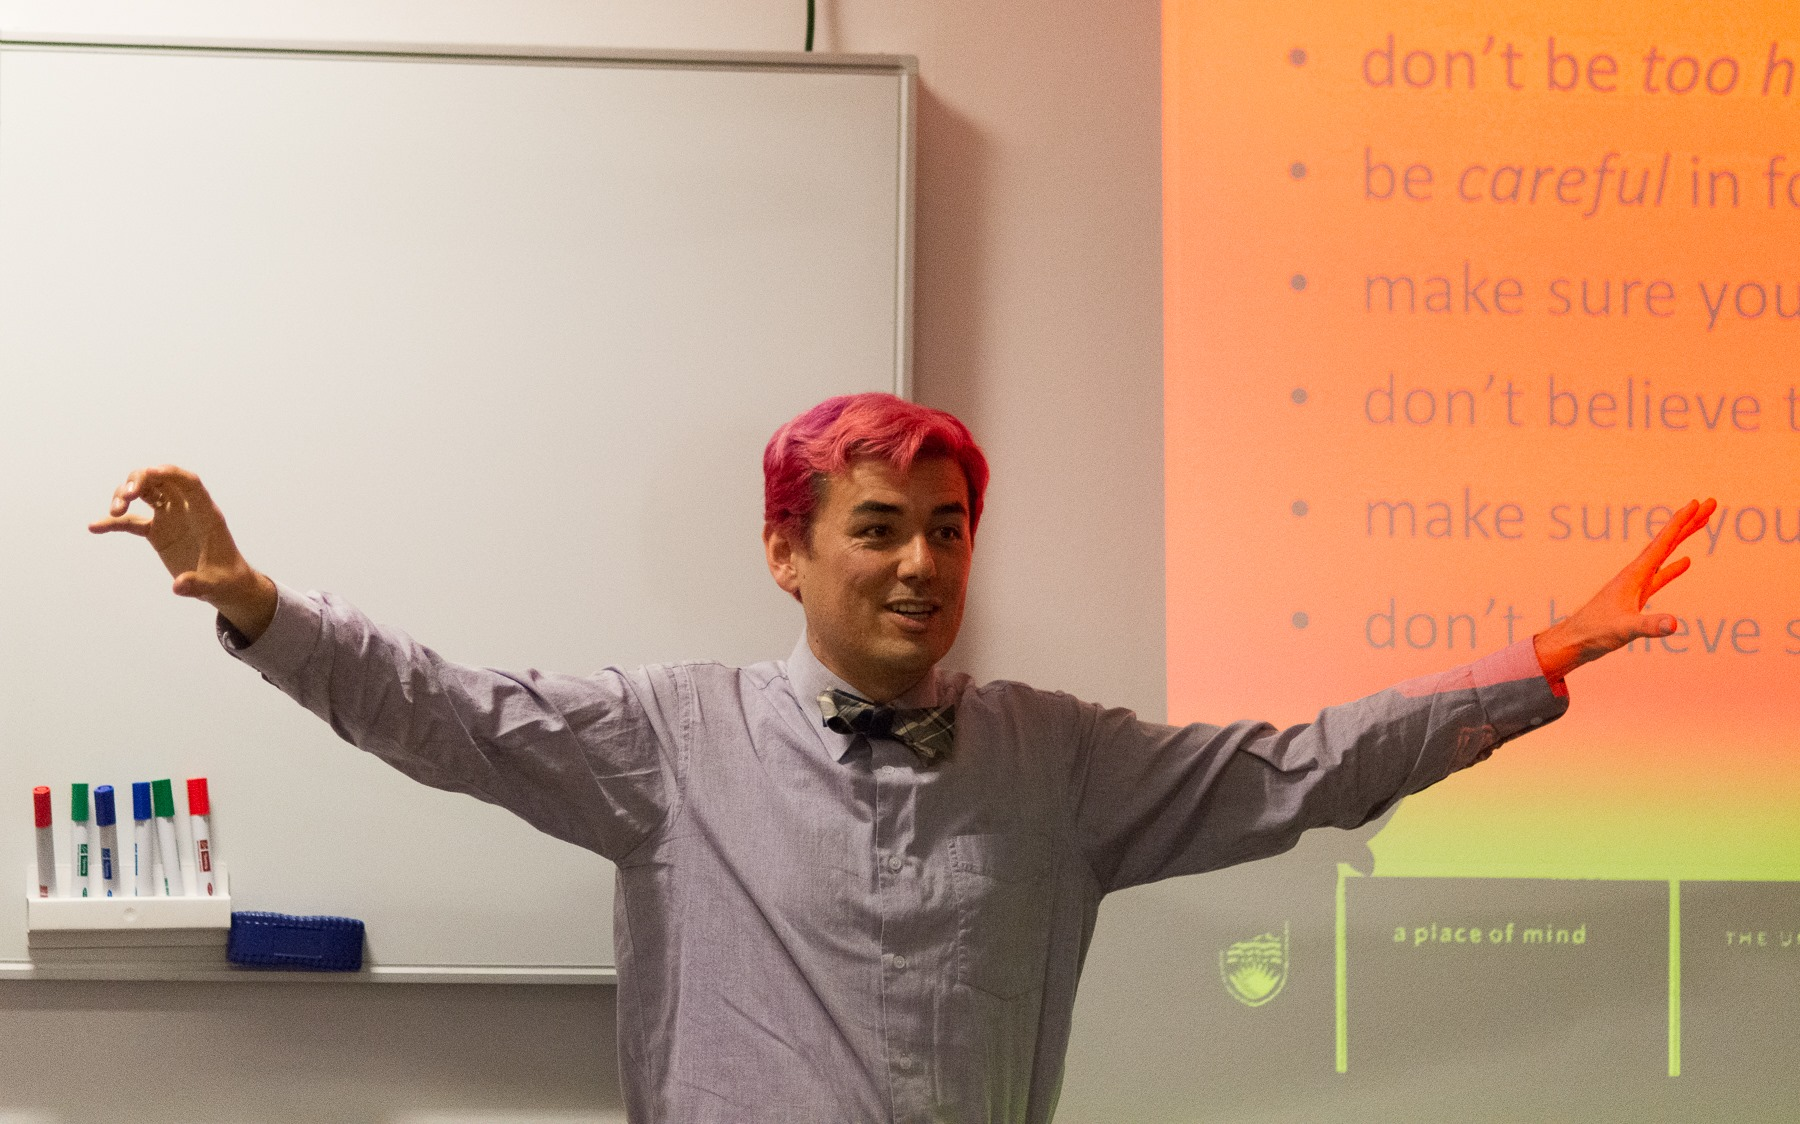
\includegraphics[width=\linewidth]{images/ichikawa.jpg}
  \centering
\end{figure}
\fi

{\sf
Jonathan Ichikawa, who modified the Magnus edition to create this version, would, first and foremost, like to thank P.D.\ Magnus. He is also grateful to Greg Restall, and his book \emph{Logic}, which is the first text he taught from and which is the model for the discussion of trees. He also thanks the many UBC students who test-drove drafts of the book. He's also grateful for helpful conversations with Roberta Ballarin, Roy Cook, Josh Dever, Dave Gilbert, Thony Gillies, and Jon Shaheen.

The original author, P.D.\ Magnus, would like to thank the people who made this project possible. Notable among these are Cristyn Magnus, who read many early drafts; Aaron Schiller, who was an early adopter and provided considerable, helpful feedback; {and} Bin Kang, Craig Erb, Nathan Carter, Wes McMichael, Selva Samuel, Dave Krueger, Brandon Lee, Toan Tran, and the students of Introduction to Logic, who detected various errors in previous versions of the book.
}

\vfill
{
\copyright\ \ifthenelse{\year=2005}{\number\year}{2005--\number\year} by P.D. Magnus and Jonathan Ichikawa. Some rights reserved.
}

{\footnotesize
You are free to copy this book, to distribute it, to display it, and to make derivative works, under the following conditions: (a) Attribution. You must give the original author credit. (b) Share Alike. If you alter, transform, or build upon this work, you may distribute the resulting work only under a license identical to this one. --- For any reuse or distribution, you must make clear to others the license terms of this work. Any of these conditions can be waived if you get permission from the copyright holder. Your fair use and other rights are in no way affected by the above. --- This is a human-readable summary of the full license, which is available on-line at \url{http://creativecommons.org/licenses/by-sa/3.0/}

Typesetting was carried out  in \LaTeX$2\varepsilon$. The style for natural deduction proofs is based on fitch.sty (v0.4) by Peter Selinger. Tree typesetting from prooftrees (v0.6) by Clea F. Rees. This copy of \forallx\ is current as of \today.
}


\pagestyle{prefacestyle}

%!TEX root = forallx-ubc.tex

\chapter*{Preface to the Fall 2023 MIT Edition}
\label{ch.preface2}
\addcontentsline{toc}{chapter}{Preface to the MIT edition}

The goal of this modified version of Ichikawa's \textit{ForAllX} is to bring some of the best features of the \textit{Logic Book}, for free!
Of the existing free texts, Ichikawa's version seemed the closest.
Why the \textit{Logic Book} system? 
It seems to strike the best balance of intellectual and practical virtues: no special symbols or special rules, a pleasing symmetry between introduction and elimination rules that makes things easy to remember, and the philosophical advantages of using proof-by-cases for disjunction elimination. 

Below is an ongoing list of modifications that have been made to Ichikawa's version, starting with some of the bigger changes.
I have maintained the list of changes that Josh has included, making a number additions.

\begin{itemize}
  \item Chapter 0 has been largely rewritten to provide a more compelling description of the subject matter of logic, and to remove some distracting glosses which may easily be misunderstood and confuse the introduction of the topic.
  \item Chapter 1 has also been substantially rewritten, clarifying the use of schematic variables in the definition of the wffs of SL, fixing conventions for dropping parentheses and quotes, and polishing examples throughout.
  \item Chapter 2 has been revised, explaining the relationship between validity in English and valid regimentations. The connection between interpretations of the language and the lines on a truth table has been clarified and certain examples have been modified or removed to avoid confusion. Validity of argument schemata has also been avoided, focusing on the validity of SL arguments themselves.
  \item Chapter 3 has been rewritten, including an explicit definition of satisfaction, defining logical entailment and unsatisfiability in these terms. Consideration of the weakening principle has been added and the relationship between validity and entailment has been clarified. Connections between consistency and satisfiability are then explained.
  \item Chapter 4 has been revised for consistency, simplifying the proof rules and definitions.
  \item Chapter 5 has been substantially rewritten, fixing errors and including proofs of soundness and completeness. The chapter begins with an expanded discussion of mathematical induction.
  \item Chapter 6 has been reordered, condensed, and substantially rewritten.
  \item Chapter 8 has been largely rewritten, eliminating reference to a UD (universe of discourse), including recursive definitions of free and bound variables, clearly distinguishing between sentences and wffs, and otherwise adapting the conventions for consistency and elegance.
  \item Chapter 9 has been completely rewritten to include a standard semantics for first-order logic which does not take constants to be rigid designators and defines true relative to both a model and variable assignment, before defining truth at a model for sentences. Minimal models have been carefully motivated and presented along with a range of techniques for establishing entailments as well as evaluating sentences on a given model.
  \item Chapter 10 has been largely rewritten to reflect the same semantic conventions presented in Chapter 9. The motivations for adding identity to the language have been connected to ideas about the logical and non-logical terms of the language. Definitions of free-for and substitution has been included and discussions of inequality quantifiers, cardinality quantifiers, definite descriptions, and Leibniz's law have been added or adjusted.
  \item Chapter 11 has been... substitution is defined and used to articulate the quantifier rules in a standard manner.
  \item Rather than calling sentence letters of SL \textit{atomic}, this label has been saved for the simplest English sentences that one can symbolise with a sentence letter in SL as well as for the simplest wffs and sentences in QL.
  \item Natural Deduction in Sentential Logic: Ichikawa's system has been modified to be in complete accordance with that in the \textit{Logic Book}.
    This mainly involves relegating Disjunctive Syllogism to a derived rule, and modifying the justification syntax for indirect proofs.
    Expository material from the Calgary edition of ForAllX has also been included.
  \item To help integrate the text better with the online \textit{Carnap} proof checker, the syntax in the Selinger Fitch system has been adapted to mirror what students must enter into \textit{Carnap} for Natural Deduction proofs in system LogicBookSD.
    One simply changes the \verb|\by{}{}| command to print the arguments in the opposite order, along with adding a colon first.
    The commands \verb|\pr{}| and \verb|\as{}| have been added for premises and subproof assumptions.
    Unfortunately, the \textit{Carnap} systems are very sensitive to syntax, and it seems cruel to ask students to learn a separate syntax for homework problems than the one they are reading in the text. %(I have also made the style file compatible with Kl{\"u}wer's Fitch system, but I don't recommend it, since it cannot be easily reformatted).
  \item The quantifier/bound variable syntax has been adapted to match that of the \textit{Logic Book}.
    System LogicBookPD accepts only `$(\exists x$)' and not `$\exists x$'.
    To avoid this tedium in the future, all quantifier/bound variable instances are written with a command \verb|\qt{}{}| whose first argument takes the quantifier and second argument takes the bound variable.
    This way, one can easily modify the formatting in the style file (e.g. removing or adding parentheses).
    Again, it would seem cruel to ask students to remember that while in \textit{Carnap} using system LogicBookPD, they MUST put parentheses around $\exists x$ and $\forall x$, if that's not the format they're seeing in their text.
  \item The recursive definition of truth-conditions in Quantifier Logic (QL) (\S\ref{sec:satisfactionQL}) have been reworked.
    Hopefully this makes it both (1) easier to understand and (2) slightly more precise.
    Whereas Ichikawa refers to this aspect of formal semantics as giving a definition of `truth', it is more accurate to say that we are defining `truth-conditions'.
    The truth-conditions for SL have been reworked in a similar vein.
  \item A more detailed list of rule schemas for SL tree rules have been included in the appendix. 
  \item The UBC edition tends to use the past-tense in a lot of places where the present-tense sounds better.
    It is part of the conceptual grammar of logic (and mathematics) that it is timeless. 
    The number of semi-colons and exclamation marks have also been reduced.
  \item Chapters have been rearranged and re-numbered so as to match the week numbers at MIT, starting with a half-week `0.'
    This way, most chapter numbers, week numbers, and problem set numbers coincide.
    Hopefully, this makes it easier to remember what we have to do each week.
\end{itemize}

If you find any errors throughout this text, please let me know and I'll happily fix them.

\begin{flushright}
Benjamin Brast-McKie \\
July 2023 \\
brastmck@mit.edu
\end{flushright}


\chapter*{Preface to the UBC Edition}
\label{ch.preface}
\addcontentsline{toc}{chapter}{Preface to the UBC edition}

\textit{The following first person pronouns refer to Ichikawa, not me! This is true for many of the first person pronouns in the book.}

This preface outlines my approach to teaching logic, and explains the way this version of \emph{forall x} differs from Magnus's original. The preface is intended more for instructors than for students. 

I have been teaching logic at the University of British Columbia since 2011; starting in 2017, I decided to prepare this textbook, based on and incorporating much of P. D. Magnus's \emph{forall x}, which has been freely available for use and modification since 2005. Preparing this text had two main advantages for me: it allowed me to tailor the text precisely to my teaching preferences and emphasis, and, because it is available for free, it is saving money for students. (I encourage instructors to take this latter consideration pretty seriously. If you have a hundred students a year, requiring them each to buy a \$50 textbook takes \$5,000 out of students' pockets each year. If you teach with this or another free book instead, you'll save your students \$50,000 over ten years. It can be sort of annoying to switch textbooks if you're used to something already. But is staying the course worth \$50,000 of your students' money?)

This text was designed for a one-semester, thirteen-week course with no prerequisites. At UBC, the course has quite a mix of students with diverse academic backgrounds. For many it is their first philosophy course. As I teach Introduction to Formal Logic, the course has three central aims: (1) to help students think more clearly about arguments and argumentative structure, in a way applicable to informal arguments in philosophy and elsewhere; (2) to provide some familiarity and comfort with formal proof systems, including practice setting out formal proofs with each step justified by a syntactically-defined rule; and (3) to provide the conceptual groundwork for metatheoretical proofs, introducing the ideas of rigorous informal proofs about formal systems, preparing students for possible future courses focusing on metalogic and computability. I try to give those three elements roughly equal focus in my course, and in this book.

The book introduces two different kinds of formal proof systems --- analytic tableaux (`trees') and Fitch-style natural deduction. Unlike many logic texts, it puts its greater emphasis on trees. There are two reasons I have found this to be useful. One is that the algorithmic nature of tree proofs means that one can be assured to achieve successful proofs on the basis of patience and careful diligence, as opposed to requiring a difficult-to-quantify (and difficult-to-teach) `flash of insight'. The other is that the soundness and completeness theorems for tree methods are simpler and more intuitive than they are for natural deduction systems, and I find it valuable to expose students to proofs of significant metatheoretical results early in their logical studies. (I prove soundness and completeness for a sentential logic tree system in the fifth week of the semester.) As presented here, the soundness and completeness proofs emphasize contrasting the systems students learn with hypothetical alternative systems that modify the rules in various ways. A rule like this would undermine the soundness of the system, but not its completeness. If we changed the rules in this way, it would still be both sound and complete. Etc. This helps give intuitive substance to these theorems.

I also include a Fitch-style natural deduction system, both for sentential and quantified logic, both because its premise-conclusion form is particularly helpful for thinking about informal arguments, and because it is important to recognize and follow proofs laid out in that kind of format, for example in more advanced philosophical material. While students do learn to do Fitch-style proofs, I emphasize less of that puzzle-solving kind of skill here than in many textbooks.

The book begins with a systematic engagement with sentential logic in conventional ways: translations, sentential connectives, models, truth tables, and both proof systems, including soundness and completeness for the tree system. Students are thereby able to familiarize themselves with all the central metalogical ideas, incorporating relatively simple logical symbolism, before introducing predicates, quantifiers, and identity. Once we enrich the language, we go through those previous ideas again, using our more complex vocabulary.

The first book I used for teaching was Greg Restall's \emph{Logic} (McGill--Queen's University Press, 2006), which I used for several years. My approach to teaching logic is heavily informed by that book; its influence in this text is particularly clear in the discussion of trees. (The natural deduction system I use is rather different from Restall's.)

In preparing this text, I began with Magnus's original and edited freely. There are sections where Magnus's prose has been retained entirely, and many of the exercises I have taken unchanged from the original. But I have also restructured many things and added quite a bit of new material. Unlike my version, which focuses on sentential logic before introducing predicates and quantification, Magnus's version integrated the discussion of sentential and quantificational systems, e.g.\ covering translation for both before discussing models and proofs for either. The original also did not include trees or soundness and completeness proofs. The two chapters on trees (\ref{ch.sl.trees} and \ref{ch.QLTrees}) and soundness and completeness (\ref{ch.SLsoundcomplete} and \ref{ch.QLsoundcomplete}) were written from scratch; my chapter on identity (\ref{ch.identity}) is also original. The other material in this edition incorporates Magnus's original material, some parts more heavily edited than others. I have slightly modified Magnus's natural deduction rules.

After a couple of years working with `beta' versions of the text online, I released the 1.0 version, along with the source code, in December 2018. The 2.0 version is new in summer 2020. The biggest changes in the latest round of revisions are in Chapter \ref{ch.ND.proofs}, where the order of presentation of the natural deduction rules has changed, and more examples have been added within the text. The rationale of the change was to start illustrating proofs earlier in the presentation of the rules. I've also put a bit more emphasis on the importance of exact matching of rule forms, and written a bit more precisely about the difference between SL proofs and proof schemas, when discussing derived rules. The other slightly substantive change I've made is to attend more precisely to how I'm using the term `interpretation' in the formal semantics for SL and QL. One of my aims is to emphasize the continuity between the two languages --- in my system, QL is literally a generalization of SL, and definitions of truth, entailment, etc., can be preserved. Various other smaller changes have been made as well, mostly stylistic changes and typo corrections. In summer 2021, I standardized and slightly modified the notation for assumptions in natural deduction proofs. I frequently make quite small corrections; the latest version is always on Github.

Many thanks, first and foremost, to P.D.\ Magnus for providing this wonderful resource under a Creative Commons license, which made it freely available and gave me the right to modify and distribute it under the same licensing agreement. I hope other instructors will also feel free to either teach directly from this version, or to modify it to develop their own. The typesetting for trees is via Clea F.\ Rees's prooftrees package; thanks to her for making it available.

I'm grateful to the students in my 2017--20 PHIL 220 courses at UBC, who had an in-progress version of this book as their course textbook. They patiently and helpfully found and pointed out mistakes as I wrote them (incentivized, perhaps, by an offer of extra credit); this version has many fewer errors than it otherwise would have had. Thanks also to Cavell Chan and Joey Deeth, who did careful proofreading, and generated many solutions to exercises for the answer key, and to Laura Greenstreet for LaTeX and other technical help. These three assistants were supported by a UBC Library Open Access Grant in 2018--19.

I am maintaining a list of known issues and errors for this book, to be corrected in future editions, under `issues' at \url{https://github.com/jonathanichikawa/for-all-x}. If you see any mistakes, please feel free to add them there directly, or to email me with them. The most recent version of the book is also always available for download there too.

\begin{flushright}
Jonathan Ichikawa \\
University of British Columbia \\
October 2021 \\
ichikawa@gmail.com
\end{flushright}


\pagestyle{mainmatter}


%!TEX root = forallx-ubc.tex
\chapter{What is logic?}
\label{ch.intro}

Logic is the business of evaluating arguments, sorting good ones from bad ones. In everyday language, we sometimes use the word `argument' to refer to belligerent shouting matches. If you and a friend have an argument in this sense, things are not going well between the two of you. This is not the kind of `argument' that will concern us. Arguments in the logical sense aren't events that happen between people; a logical argument is structured to give someone a reason to believe some conclusion on the basis of the premises. Here are two examples:

\label{argRaining}
\begin{earg}
  \item[(1)] It is raining heavily.
  \item[(2)] When it rains, everyone outside without an umbrella gets wet.
  \item[\therefore] You should take an umbrella.
\end{earg}


\label{argSnowing}
\begin{earg}
  \item[(1)] It is either raining or snowing.
  \item[(2)] If it is colder than -10 degrees, it is not raining.
  \item[(3)] It is -18 degrees.
  \item[\therefore] It is snowing.
\end{earg}
 
The three dots on the last line of each argument mean \textit{therefore}, and they indicate that the final sentence is the \textsl{conclusion} of the argument. The other sentences are the \textsl{premises} of the argument. If you believe the premises, then the argument provides you with a reason to believe the conclusion.

This chapter discusses some basic logical notions that apply to arguments in a natural language like English. It is important to begin with a clear understanding of what arguments are and of what it means for an argument to be valid. Later we will translate arguments from English into a formal language. We want formal validity, as defined in the formal language, to have at least some of the important features of natural-language validity.

\section{Arguments}
A crucial part of analyzing an argument is identifying its conclusion. Every argument has a conclusion --- the conclusion is the claim the argument aims to establish. Premises are starting-points, used to lend support to the conclusion. Often, the conclusion will be signified by words like `so' or `therefore'. Premises might be marked by words like `because'. These words can give a clue as to just what the argument is supposed to be.

\begin{description}
  \item[premise indicators:] since, because, given that
  \item[conclusion indicators:] therefore, hence, thus, then, so
\end{description}

In a natural language like English, \emph{sometimes}, arguments start with their premises and end with their conclusions, but not always. For some purposes in this course, we will be working with \emph{idealizations} of natural language, where we work as if some generally applicable rules of thumb held without exception. Let's define (a slightly technical notion of) an \define{argument} as a sequence of sentences. The sentences at the beginning of the sequence are premises. The final sentence in the sequence is the conclusion.

Here is an example of an argument:

\begin{earg}
  \item[] People get wet whenever it rains.
  \item[] It often rains in Vancouver.
  \item[\therefore] People often get wet in Vancouver.
\end{earg}

The idea of an argument is that the premises are supposed to give you reason to accept the conclusion (or more generally, to increase your degree of confidence in the conclusion). If I'm trying to convince you that people often get wet in Vancouver --- the conclusion of the argument above --- convincing you of the two premises might be a good way to get you there.

Notice that our definition of an argument is quite general. Consider this example:
\begin{earg}
  \item[] Vancouver has more churches than any other Canadian city.
  \item[] Two oboes are fighting a duel under the fireworks (watch out!).
  \item[\therefore] J.\ Edgar Hoover was an honest man, allegedly.
\end{earg}

It may seem odd to call this an argument, but that is because it would be a {terrible} argument. The two premises have nothing at all to do with the conclusion. (Moreover, they aren't very plausible.) Nevertheless, given our definition, it still counts as an argument --- albeit a bad one. One of our central aims in formal logic is to provide rigorous, formal tests for evaluating deductive arguments. \textit{Deductive arguments} aim to establish a conclusion beyond a reasonable doubt. In contrast, \textit{inductive} arguments aim to simply increase our degree of confidence in a conclusion (this includes `abductive' reasoning, i.e. inference to the best explanation). 

For better or worse, we will have almost nothing to say about inductive arguments in this course.\footnote{We \textit{will} consider an entirely different style of reasoning called `proofs by induction' where---confusingly---`induction' means something TOTALLY different. So few good words to go around, so many good ideas!} This is despite the fact that much of science and ordinary life operates using inductive rather than deductive reasoning. The good news is that our systems will be versatile and have some elegant formal properties. Inductive logic is still struggling to achieve comparable riches. Furthermore, deductive logic is of vital importance for mathematics and computer science, significantly reshaping the world we live in by making the rise of the information age possible. Apart from its various technical applications, deductive logic sets an ideal for reasoning that we can aspire to achieve in daily life.


\section{Sentences and Propositions}
\label{intro.sentences}

The premises and conclusions of arguments are sentences. But not just any English sentence is suitable for figuring into an argument. For example, questions count as grammatical sentences of English, but logical arguments never have questions as premises or conclusions. We are interested especially in sentences that can be true or false. Think of these as the sentences that purport to describe the way things are. Such sentences are sometimes described as expressing \emph{propositions}. The English sentence `snow is white' expresses the same proposition as the German sentence `Schnee ist wei\ss.' Both express the fact that snow is white. The \define{truth-value} of a sentence settles whether it is true or false.

%We will call truth or falsity the \define{truth-value} of a sentence.

We will not theorize about questions or other non-propositional sentences in formal logic. Since we are only interested in sentences that can figure as a premise or conclusion of an argument, we'll define a technical notion of a \define{sentence} as a grammatical string of symbols that expresses a proposition which is either true or false. Such strings are often referred to as \textit{declarative sentences}, though for brevity we will drop `declarative' throughout.

When we say that `a sentence can be true or false,' all we really require is that we can intelligibly assign a truth-value to it. There are many sentences where it is unclear---or at least highly controversial---whether they have a truth-value independently of conscious agents. Think of sentences such as `Almonds are yummy' or `the U.S.\ invasion of Iraq was unjustified'. In an argument, we can assign a truth-value to such sentences, even if some of us might be skeptical that they have a truth-value just sitting out there, in some Platonic realm. Our system will handle these sentences just like sentences whose content seems more `objective', such as the sentence `you are reading a logic book right now.' Indeed, often what is at stake in our more interesting arguments is whether various normatively-loaded claims are true or false. So clearly, we have some way of reasoning about them using truth-values. Whether there's anything more to be said is beyond the scope of \textit{this} course.

%Ichikawa: Don't confuse the idea that a sentence can be true or false with the difference between fact and opinion. Often, sentences in logic will express things that would count as facts --- such as `Kierkegaard was a hunchback' or `Kierkegaard liked almonds.' They can also express things that you might think of as matters of opinion --- such as, `Almonds are yummy' or `the U.S.\ invasion of Iraq was unjustified'. These are all examples of things that are either true or false.
% JH: But what does it mean to say that the opinion-sentences are true or false? Does this  na\"ively commit us to a kind of realism about their contents?

It is also important to keep clear the distinction between something's being \emph{true} and something's being \emph{known}. A sentence is the kind of thing that can be true or false; that doesn't mean you'll always be able to tell whether it is true or false. For example, `there are an even number of humans on Earth right now' is a sentence. It is either true or false, even though it is pretty much impossible to tell which. Similarly, there are controversial propositions, where people disagree about whether they are true or false, and where it seems very difficult to settle the debate. For the sake of an argument, we may treat controversial propositions as true (or false) in order to see what follows as a result, and indeed many arguments do so. 
% JH: not sure about the humans example. There are issues of vagueness regarding both conjoined twins and also when humans come into existence (e.g. at what point does a baby have to exit the womb? do late-stage fetuses count as babies and if so when)

What are some examples of grammatical English sentences that do not express propositions? We've discussed one category already:

\paragraph{Questions} In a grammar class, `Are you sleepy yet?' would count as an interrogative sentence. Whether you are sleepy or not, the question itself is neither true nor false. Thus `Are you sleepy yet?' is not a sentence in our technical, propositional sense. Suppose you answer the question: `I am not sleepy.' This \emph{is} either true or false, and so \emph{is} a sentence in the logical sense. Generally, \emph{questions} will not count as sentences, but \emph{answers} will. 

`What is this course about?' is not a sentence, but `No one knows what this course is about' is a sentence.

\paragraph{Imperatives} Commands are often phrased as imperatives like `Wake up!', `Sit up straight', and so on. In a grammar class, these would count as imperative sentences. Although it might be good for you to sit up straight or it might not, the command is neither true nor false. Note, however, that commands are not always phrased as imperatives. `You will respect my authority' \emph{is} either true or false --- either you will or you will not --- and so it counts as a sentence in the logical sense.

\paragraph{Exclamations} Expressions like `Ouch!' or `Boo, Yankees!' are sometimes described as exclamatory sentences, but they are neither true nor false. We will treat `Ouch, I hurt my toe!' as meaning the same thing as `I hurt my toe.' The `ouch' does not add anything that could be true or false.

To recap: \emph{sentences}, in the technical sense we're interested in, are claims that can be true or false. One pretty good test you can run to see whether something is a sentence is to ask whether it makes sense to insert `It is true that' or `It is false that' in front of it. It's perfectly fine to say `It is true that Kierkegaard liked almonds' or `It is true that the U.S.\ invasion of Iraq was unjustified'. But it doesn't make sense to say `It is true that are you sleepy yet' or `It is true that sit up straight'.





\section{Logical Validity}

There are two important ways that arguments can go wrong.
To begin with, suppose that the following argument were presented in a court of law:

\begin{earg}
  \item[(1)] The victim was shot by a bullet from the gun that was found at the defendant's house.
  \item[(2)] The fingerprints on the gun were shown to match the defendant.
  \item[(3)] The gun was registered in the defendant's name.
  \item[(4)] The defendant had recently been fired by the victim.
  \item[\therefore] The defendant shot the victim.
\end{earg}

An argument is only compelling if its premises are true.
If the premises above can be shown to be false, the defendant may well be innocent.
More generally, we should not feel at all persuaded to believe a conclusion on the basis of an argument with false premises. 
This is the first way that an argument can go wrong: not all of the premises are true.

Assuming that the premises (1) -- (4) are true, the conclusion would seem to follow.
What we mean by `follow' in this instance is that the truth of the premises makes the truth of the conclusion extremely likely, and perhaps so likely that it is beyond a reasonable doubt, compelling the jury to find the defendant guilty.

What may be good enough for the law is not good enough for logic.
This is not to disparage the criminal justice system but to observe that the truth of the conclusion in the argument above does not follow \textit{logically} from the truth of its premises.
However likely the conclusion may be given the truth of its premises, it is still \textit{possible} for the premises to be true and the conclusion false.
For instance, consider a possibility in which it was the defendant's partner who shot the victim.
Even though all of the premises are true, the conclusion is false in such a possibility.
We may not know if that possibility is what happened or not, but it doesn't matter.
So long as it is possible for the premises to be true and the conclusion to be false we have reason to deny that the conclusion follows logically from its premises.

Is this what logical validity is about: ruling out \textit{possibilities} in which the premises are true and the conclusion is false where possibilities are ways for things to be?
No!
Let's take a look at some arguments which take this form, ruling out any possibility in which the premises are true and the conclusion is false:

\begin{earg}
  \item[(1)] The atom is gold
  \item[\therefore] The atom has 79 protons.
\end{earg}


\begin{earg}
  \item[(1)] Suela is a fox (the animal).
  \item[(2)] Suela is female.
  \item[\therefore] Suela is a vixen.
\end{earg}

In both of the arguments above, every possibility in which premises are true is one in which the conclusion is true.
Assuming the premises are true, the conclusion follows as a matter of necessity.
Put otherwise, the truth of the premises \emph{necessitate} the truth of their conclusions.
Certainly these are stronger arguments than what we might find in a court of law.
Are there arguments that are even more powerful than this?
The answer is `yes', and this brings us to the topic of this course.
Consider the following arguments:

\begin{earg}
  \item[(1)] Socrates is a man.
  \item[(2)] Every man is mortal.
  \item[\therefore] Socrates is mortal.
\end{earg}

Here too the premises necessitate the conclusion since there is no possibility in which the premises are true and the conclusion is false.
However, unlike the previous arguments, we do not need to know what `Socrates', `man', or `mortal' mean.
In order to get a sense of this, let's consider one more argument:

\begin{earg}
  \item[(1)] Gyre is a mome rath.
  \item[(2)] All mome raths are slithy.
  \item[\therefore] Gyre is slithy.
\end{earg}

Even without knowing who Gyre is, anything about mome raths, or what it is to be slithy, we may say with equal certainty that it is not possible for the premises to be true and the conclusion false.
In fact we can say more than this: there is no \textit{interpretation} of the premises and conclusion where the former are true and the latter is false.
So what's an interpretation?

We will provide a precise definition of what an interpretation is in setting up semantic theories for the languages that we will study throughout this course (chapters $\ref{ch.TruthTables}$, $\ref{ch.SLmodels}$, and $\ref{ch.QL.models}$).
For the time being, it will help to get some sense of an informal analogue with which we are already familiar.
To do so, let's return to the gold argument from before.

Surly any possibility in which the atom is gold is also one in which the atom has 79 protons.
After all, having 79 protons is part of what it is to be gold, and so something couldn't be gold without having 79 protons.
Who could argue with that?

Although no one should balk at the gold argument given the normal interpretation of its sentences--- what is often called the \textit{intended interpretation}--- the same cannot be said if we entertain unintended interpretations.
For instance, suppose we were to take `gold' to mean what `carbon' means in the intended interpretation, that is: carbon.
What the premise means on this unintended interpretation could equally be said by an intended interpretation of the sentence `The gold atom is carbon'.
Since carbon only has 6 protons and not 79, the conclusion is false when the premise is true on this unintended interpretation.
But why should we care about unintended interpretations?
Shouldn't we restrict attention to just the intended interpretations of our sentences that we are accustomed to using?

The reason for considering all interpretations and not just the intended one(s) we seem to most of the time is that it allows us to distinguish a uniquely strong type of argument that holds independent of how we choose to interpret our language.
Although we will improve on this characterisation in later chapters, we may nevertheless draw on an intuitive understanding of the interpretations of our language to say that what it is for an argument to be \define{logically valid} is for the conclusion to be true on any interpretation in which all of the premises are true. 
Functionally, it is helpful to think of logically valid arguments as arguments that can be relied on no matter how (or whether) you understand the non-logical terms like `is gold' or `Socrates' with which the argument is stated.
So even though the gold argument is extremely compelling when we maintain the intended interpretation of our language that we are all accustomed to, the gold argument is not a logically valid argument: there is an interpretation of the language in which its premise is true and its conclusion is false.

We have identified the second way that an argument can go wrong: it can admit of an interpretation in which the premises are true but the conclusion is false.
Recall Gyre and those slithy mome raths from before.
We may not know much about these sorts of things, but we can be sure that Gyre is slithy if Gyre is a mome rath where all mome raths are slithy.
We may know considerably more about Socrates being male and mortal, but similar reasoning applies.
Indeed, these two arguments may be observed to have the same \textit{logical form}.
It is these logical forms of reasoning that will be the topic of this course.

When an argument has neither of the defects considered above--- i.e., when it is both logically valid and has true premises (on the intended interpretation)--- we may say that it is \textit{sound}.\footnote{As we will see, there is an entirely distinct notion of \textit{soundness} pertaining to our proof systems.}
Sound arguments are a good thing, but fall outside the scope of this course.
Why is that?
Because securing the truth of the premises is often an empirical (or in general extra-logical) matter and presumes that a single interpretation is to be privileged over the others.
Rather, we will only be concerned with identifying which arguments are logically valid, not which interpretation we should focus on or which premises are true on that interpretation.
We will also exclude consideration of a wider understanding of valid arguments which includes arguments that are really convincing--- e.g., in a court of law--- but not logically valid.
Accordingly, we will typically drop `logically' in talking about logically valid arguments, referring to arguments simply as \textit{valid} or, when they are not valid, as \textit{invalid}.

A parting question: how would you begin to describe the space of all valid forms of reasoning? 
It is a great intellectual achievement of the late 19th and early 20th centuries that we have devised systematic methods for answering this question (relative to a language).
In this course we will consider two types of answers, one belonging to proof theory, and the other belonging to model theory (also called semantics).
In the metalogical portions of this course, we will show how these two methods deliver the same answer, describing one and the same space of valid forms of reasoning despite doing so in radically different ways.





\section{Logical Form}
\label{sec:LogicalForm}

We've seen that a valid argument does not need to have true premises or a true conclusion.
Conversely, having true premises and a true conclusion is also not enough to make an argument valid.
Consider this example:

\begin{earg}
  \item[] Ted Cruz is a U.S.\ citizen.
  \item[] Justin Trudeau is a Canadian citizen.
  \item[\therefore] UBC is the largest employer in Vancouver.
\end{earg}

The premises and conclusion of this argument are, as a matter of fact, all true.
Nevertheless, this is quite a poor argument.
In particular, the definition of validity is not satisfied: there are interpretations in which the premises are true while the conclusion is false.
Although the conclusion is true on the intended interpretation, this may fail to hold on other interpretations.
For example, we may interpret `UBC' to mean what `Lululemon' does on the intended interpretation.
Accordingly, the premises are true, and yet the conclusion is false.

The important thing to remember is that validity is not about the truth or falsity of the sentences in the argument on any particular interpretation. 
Instead, it is about the \textit{logical form} of the argument.
But what is the logical form of an argument?

We have begun to see some valid arguments like the Socrates argument and the Gyre argument.
But was that one argument or two?
Recall that an argument is a sequence of sentences in which the last sentence is the conclusion.
Since the sentences in the Socrates and Gyre arguments differed, they are different arguments.
Nevertheless, they shared the same logical form.
Here is a valid argument with a different logical form:

\begin{earg}
  \item[(1)] Oranges are either fruits or musical instruments.
  \item[(2)] Oranges are not fruits.
  \item[\therefore] Oranges are musical instruments.
\end{earg}

This is a valid argument: there is no interpretation in which the premises are true and the conclusion is false.
Since, given the intended interpretation, it has a false premise --- premise (2) --- it does not actually establish its conclusion, but it does have a valid \emph{logical form}.
Here is one more example of an argument with a valid logical form:

\begin{earg}
  \item If it is raining, then the streets are wet.
  \item The streets are not wet.
  \item[\therefore] It is not raining.
\end{earg}

As we will see, there are many logical forms that arguments can have.
In order to characterise the abstract forms themselves, we will use variables.
To begin with, we will restrict our variables to sentences, calling these \textit{sentential variables}.
Without introducing any notation beyond sentential variables, we may represent the previous argument form as follows:

\begin{earg}
  \item If $\metaA{}$, then $\metaB{}$.
  \item It is not the case that $\metaB{}$.
  \item[\therefore] It is not the case that $\metaA{}$.
\end{earg}

Instead of an argument itself, what we have above is a recipe where substituting any sentences whatsoever for the variables `$\metaA{}$' and `$\metaB{}$' yields an argument that, like the raining argument, is valid.\footnote{We will have more to say about the `\metaA{}' notation in the `note about notation' on p.\ \pageref{notationnote}.}
By replacing sentences with variables, we were able to abstract away the non-logical parts of the raining argument, leaving behind the logical form of the original raining argument.
We may refer to the result as an \textit{argument schema}.
Argument schemata are built up out of two elements: variables (in this case sentential variables) and \textit{logical constants}.
The logical constants included above were represented using `If\ldots, then\ldots' and `It is not the case that\ldots'.
We will introduce more elegant representations of these logical constants soon.
Until then, it is worth considering if we can identify an argument schema for the Socrates argument in the very same way?
Yes, but we need more than sentential variables to do so.

Suppose that we were to maintain our restriction to sentential variables from before.
The plan is to replace sentences with variables and try to recover a valid argument form just like we did before.
Since `Socrates is a man' is a sentence and doesn't have any parts that are also sentences (we say it is \textit{atomic}), all we can do is replace it with a variable.
Let's choose `$\metaA{}$' for this. 
We find something similar for the second premise `Every man is mortal'.
Let's choose the variable `$\metaB{}$'.
Finally, the conclusion which again is as simple as sentences get, and so lets choose `$\metaC{}$'.
Thus we get the following argument schema:

\begin{earg}
  \item $\metaA{}$
  \item $\metaB{}$
  \item[\therefore] $\metaC{}$
\end{earg}

Although this does \textit{schematize} the Socrates argument, it does not leave behind anything which we might appeal to in explaining why the Socrates argument was valid.
For instance, if we replace the variables with any other sentences, we do not necessarily get a valid argument.
Have we made some mistake?
No.
Rather, the validity of the Socrates argument is not visible at the logical resolution that we have been working.
Instead of abstracting on sentences, we need to analyse the sub-sentential parts, identifying logical constants at this higher level of logical resolution.
In particular, we will need to split sentences up into predicates and singular terms, introducing logical constants for quantification like `for all' and `there is some'.
This ambition will be addressed in later chapters on Quantifier Logic (QL).
Until then, we will keep things simple to start, focusing on Sentential Logic (SL).





\section{Other Logical Notions}

Here are a few more relevant terms we'll be working with.

\subsection{Logical truths (Tautologies)}
\label{sec-tautologydef}
In considering arguments formally, we care about what would be true \emph{if} the premises were true on any interpretation where interpretations are carefully defined. 
Generally, we are not concerned with the actual truth value of any particular sentences --- whether they are \emph{actually} true or false on an intended interpretation.
Yet there are some sentences that are true on all interpretations, just as a matter of logic alone.

Compare these sentences:

\begin{earg}
  \item[\ex{Acontingent}] It is raining.
  \item[\ex{Atautology}] Either it is hot outside, or it is not hot outside.
  \item[\ex{Acontradiction}] John is sitting down and it is not the case that John is sitting down.
\end{earg}
% TODO: fix `never' above which has a temporal reading and modal reading

Sentence \ref{Acontingent} could be true or it could be false.
Sentences that could be true, or could be false, are called \emph{contingent} sentences.

Sentence \ref{Atautology} is different.
Even though I don't know what the weather is like as you're reading this book, I still know that it's just as true for you as it is for me.
Moreover, it is true no matter how you interpret `It is raining'.
Sentence \ref{Atautology} is logically true since it is true on all interpretations.
We call a sentence like this a \define{logical truth} or a \define{tautology}.

You do not need to know what John is up to, or know how to interpret sentence \ref{Acontradiction} in order to know that this sentence is false, simply as a matter of logic.
The third sentence is called \define{logically false} or a \define{contradiction}.

I said above that a contingent sentence could be true on some interpretations and false on others.
We can also define contingency in terms of tautologies and contradictions thus: a \define{contingent sentence} is a sentence that is neither a tautology nor a contradiction.

%A sentence might \emph{always} be true and still be contingent. For instance, if there never were a time when the universe contained fewer than seven things, then the sentence `At least seven things exist' would always be true. Yet the sentence is contingent; its truth is not a matter of logic. There is no contradiction in considering a possible world in which there are fewer than seven things. The important question is whether the sentence \emph{must} be true, just on account of logic.

\subsection{Logical Entailment and Equivalence}
We can also ask about the logical relations \emph{between} two sentences. For example:

\begin{earg}
  \item[] If Sunil went to the store, then he washed the dishes.
  \item[] If Sunil did not wash the dishes, then he did not go to the store.
\end{earg}

These two sentences are both contingent, and yet they have the same truth-value no matter how we interpret these sentences.
When two sentences have the same truth value on all interpretations, we say that they are \define{logically equivalent}.

Notice that both of these arguments are valid:

\begin{earg}
  \item[] If Sunil went to the store, then he washed the dishes.
  \item[\therefore] If Sunil did not wash the dishes, then he did not go to the store.
\end{earg}

\begin{earg}
  \item[] If Sunil did not wash the dishes, then he did not go to the store.
  \item[\therefore] If Sunil went to the store, then he washed the dishes.
\end{earg}

One sentence \textit{logically entails} another just in case every interpretation on which the former is true, the latter sentence is also true.\footnote{We will also consider what \textit{sets sentences} logically entail.}
We may then observe that for any valid argument with one premise, that premise logically entails its conclusion.
This is what we find in both of the arguments above.
Thus we can also define logical equivalence in terms of logical entailment: two sentences are \textit{logically equivalent} just in case they logically entail each other.




\subsection{Consistency}

Consider these three sentences:

\begin{ekey}
\item[B1] Sam is shorter than John.
\item[B2] Sam is taller than John. 
\item[B3] If Sam is shorter than John, then Sam is not taller than John.
\end{ekey}

Even without knowing the truth values of these sentences, we may determine by logical alone that there is no interpretation which makes all of these sentences true. 
For instance, we might reason as follows: suppose there were some interpretation which makes all three sentences true.
However, it follows from \textbf{B1} and \textbf{B3} that \textbf{B2} is false.
This contradicts our supposition.
Since we have arrived at a contradiction on the supposition that there was an interpretation that makes all three sentences true, we may reject our supposition: there is no interpretation which makes all three sentences true.

A set of sentences is \textit{consistent} just in case there is some interpretation which makes every sentence in the set true.
Otherwise, a set is called \textit{inconsistent}: there is no interpretation which makes every sentence in the set true.
For instance, the set $\{\textbf{B1}, \textbf{B2}, \textbf{B3}\}$ is inconsistent.

We can ask about the consistency of any set of sentences whatsoever.
Given an inconsistent set of sentences $X$, if every sentence in $X$ is also a sentence in $Y$, then $Y$ is also inconsistent. 
The opposite is not true: if every sentence in $Z$ is in $X$ and $X$ is inconsistent, it does not follow that $Z$ is inconsistent. 
Can you find which subsets of $\{\textbf{B1}, \textbf{B2}, \textbf{B3}\}$ are consistent?



% \section{Formal languages}
%
% English is a natural language, not a formal one. Its rules are vague and messy, and constantly changing. We will spend some time translating between English and our formal languages, but the translations will not always be precise. There is a tension between wanting to capture as much of the structure of English as possible and wanting a simple formal language with tractable rules --- simpler formal languages will approximate natural languages less closely. There is no perfect formal language. Some will do a better job than others in translating particular English-language arguments.
%
% In this book, we make the assumption that \emph{true} and \emph{false} are the only possible truth-values. Logical languages that make this assumption are called \emph{bivalent}, which means \emph{two-valued}. SL and QL are both bivalent, but some philosophers have emphasized limits to the power of bivalent logic. Some logics, beyond the scope of this book, allow for sentences that are neither true nor false. Others allow for sentences that are both true \emph{and} false. Our logical system, which is often called \emph{classical logic}, will give every sentence exactly one truth value: every sentence will be either true or false, and not both.


\section*{Summary of logical notions}
\begin{itemize}

\item An \define{argument} is a sequence set of sentences, with \emph{premises} (there could be no premises) followed by a \emph{conclusion}.

\item A \define{sentence}, in our logical terminology, is a grammatical string of symbols that expresses a proposition, which can be either true or false.

\item An argument is \define{valid} if the conclusion is true on every interpretation which makes all of the premises true; it is \define{invalid} otherwise.

\item A \define{tautology} is a sentence that is true on all interpretations.

\item A \define{contradiction} is a sentence that is not true on any interpretation.

\item A \define{contingent sentence} is neither a tautology nor a contradiction.

\item One sentence \define{logically entails} another just in case the latter sentence is true in every interpretation in which the former is true.

\item Two sentences are \define{logically equivalent} if they have the same truth-value on all interpretations, or put otherwise, if they logically entail each other.

\item A set of sentences is \define{consistent} if there is an interpretation which makes every sentence in that set true; it is \define{inconsistent} otherwise.

\end{itemize}


% \iffalse %moving these to separate file, so as to push to the end!

\practiceproblems
At the end of each chapter, you will find a series of practice problems that review and explore the material covered in the chapter. There is no substitute for actually working through some problems, because logic is more about a way of thinking than it is about memorizing facts. The answers to some of the problems are provided at the end of the book in appendix \ref{app.solutions}; the problems that are solved in the appendix are marked with a \solutions.

\solutions
\problempart
\label{pr.Sentences1}
Which of the following are `sentences' in the logical sense?
\begin{earg}
\item England is smaller than China.
\item Greenland is south of Jerusalem.
\item Is New Jersey east of Wisconsin?
\item The atomic number of helium is 2.
\item The atomic number of helium is $\pi$.
\item I hate overcooked noodles.
\item Blech! Overcooked noodles!
\item Overcooked noodles are disgusting.
\item Take your time.
\item This is the last question.
\end{earg}

\problempart
\label{hw1.B}
Which of the following are `sentences' in the logical sense?
	\begin{earg}
		\item I would like a double cheeseburger with no onions.
		\item Thank you very much for that gracious reception.
		\item If you strike me down, I shall become more powerful than you could possibly imagine.
		\item There are more trees at UBC than there are flowers in my office and my Uncle Jack really seems to like drinking apple juice, or if that's not apple juice, then he really seems to like whatever it is that he's drinking, but anyway, what I'm really trying to say is, I'm hungry and I could really go for a burger or a bag of scorpions right about now.
		\item I did it
		\item No invalid arguments have impossible premises.
	\end{earg}

\problempart
\label{pr.EnglishTautology}
For each of the following: Is it a tautology, a contradiction, or a contingent sentence?
\begin{earg}
\item Caesar crossed the Rubicon.
\item Someone once crossed the Rubicon.
\item No one has ever crossed the Rubicon.
\item If Caesar crossed the Rubicon, then someone has.
\item Even though Caesar crossed the Rubicon, no one has ever crossed the Rubicon.
\item If anyone has ever crossed the Rubicon, it was Caesar.
\end{earg}

% \solutions
% \problempart
% \label{pr.MartianGiraffes}
% Look back at the sentences G1--G4 on p.~\pageref{MartianGiraffes}, and consider each of the following sets of sentences. Which are consistent? Which are inconsistent?
% \begin{earg}
% \item G2, G3, and G4
% \item G1, G3, and G4
% \item G1, G2, and G4
% \item G1, G2, and G3
% \end{earg}

\solutions
\problempart
\label{pr.EnglishCombinations}
Which of the following is possible? If it is possible, give an example. If it is not possible, explain why.
\begin{earg}
\item A valid argument that has one false premise and one true premise.
\item A valid argument that has a false conclusion.
\item A valid argument, the conclusion of which is a contradiction.
\item An invalid argument, the conclusion of which is a tautology.
\item A tautology that is contingent.
\item Two logically equivalent sentences, both of which are tautologies.
\item Two logically equivalent sentences, one of which is a tautology and one of which is contingent.
\item Two logically equivalent sentences that together are an inconsistent set.
\item A consistent set of sentences that contains a contradiction.
\item An inconsistent set of sentences that contains a tautology.
\end{earg}


\problempart
\label{hw1.C}
For each, give an argument with the indicated features, or explain why it is impossible to do so:
	\begin{earg}
		\item Valid, but not sound.
		\item Valid, with a contradictory conclusion.
		\item Sound, with an contradictory premise.
		\item Sound, and an instance of this form:
			\begin{earg}
        \item[] If $\metaA{}$, then $\metaB{}$
        \item[] $\metaC{}$
        \item[\therefore] $\metaB{}$
			\end{earg}
	\end{earg}


\problempart
\label{pr.ImpossiblePremises}
Is this argument valid? Why or why not?
\begin{earg}
\item[(1)] PHIL 220 is a course with a final exam.
\item[(2)] No course has a final exams.
\item[\therefore] Everyone is going to get an A in PHIL 220.
\end{earg}

\problempart
\label{hw1.A}
For each, indicate whether it is true or false.
	\begin{earg}
		\item All arguments with true premises and true conclusions are sound.
		\item Only valid arguments are sound.
		\item If an argument with the conclusion $A$ is sound, then an argument with the conclusion not $A$ is not sound.
		\item All arguments with at least one contradictory premise are valid.
		\item No invalid arguments have contradictory premises.
	\end{earg}
	
	% \fi 


%\iffalse
%!TEX root = forallx-ubc.tex
\chapter{Sentential Logic}
\label{ch.SL}




This chapter introduces a logical language called SL.
It is a version of \emph{sentential logic}, because the basic units of the language will represent entire sentences.
(Recall from \S\ref{intro.sentences} that we're only considering declarative sentences.)
We will be concerned with translating sentences and whole arguments into SL.
This brings us to our first definition: 
  
A \define{regimentation} (also called a \define{symbolization}) of an English sentence in SL is any sentence in SL which captures (some amount of) the logical form of that English sentence.

This definition is vague, and necessarily so.
As we will see, there will typically be more than one way to regiment a sentence in English, and different regimentations may capture more or less of the English sentence's logical form.
Rather than a precise mathematical definition, regimentation (like any translation!) is a matter of degree, where some regimentations are better than others, and many may be on a par with each other.
We may then say:

A \define{regimentation} (or \define{symbolization}) of an argument in English is an argument in SL whose sentences regiment the sentences of the argument in English.

We will see a number of examples throughout this chapter, but it is good to have this definition in mind as you read, considering other ways that you might regiment the sentences and arguments in question.




\section{Sentence Letters}

In SL, capital Roman letters ($A$, $B$, $C$, etc.) are the \define{sentence letters}.
These are the basic building blocks from which complex sentences may be constructed.
Considered only as a symbol of SL, the letter `$A$' could regiment any English sentence.
So when regimenting English in SL, it is important to provide a \emph{symbolization key}.
The key provides an English language sentence for each sentence letter used in the regimentation.

For example, consider this argument:

\begin{earg}
\item[] Today is New Year's Day.
\item[] If today is New Year's Day, then people are swimming in English Bay.
\item[\therefore] People are swimming in English Bay.
\end{earg}

This is a valid argument in English.
In regimenting it, we want to preserve the logical form of the argument which makes it valid.
What happens if we replace each sentence with a letter? 
Our symbolization key would look like this:

\begin{ekey}
\item[A:]Today is New Year's Day.
\item[B:]If today is New Year's Day, then people are swimming in English Bay.
\item[C:]People are swimming in English Bay.
\end{ekey}

We could then regiment the argument in this way:

\begin{earg}
\item[] $A$
\item[] $B$
\item[\therefore] $C$
\end{earg}

This is a regimentation of the argument, but it's not a very interesting one.
In particular, our regimentation does not encode any logical connection between $A$, $B$, and $C$.
What was compelling about the original argument has been lost in translation.
Whereas the original argument was valid, the regimentation given above is not.
After all, $A$, $B$, and $C$ could be any sentences whatsoever.
Just because $A$ and $B$ are true (on a given interpretation), it does not follow that $C$ is also true (on that interpretation).\footnote{We will provide a formal definition of validity for SL in Ch.~$\ref{ch.TruthTables}$ and Ch.~$\ref{ch.SLmodels}$.}

The symbolization key provided above is by no means the only symbolization key that we could have provided.
For instance, consider the following alternative:

\begin{ekey}
\item[]Today is Christmas Day.
\item[]Tiny Tim has difficulty walking without crutches.
\item[\therefore]We're all going to die tomorrow.
\end{ekey}

A more interesting regimentation of the valid New Year's argument will show how it is different from the invalid Christmas argument.
The relevant thing about the New Year's argument is that the second premise is not just \emph{any} sentence.
Notice that the second premise contains the first premise and the conclusion \emph{as parts}.
Our symbolization key for the argument only needs to include meanings for $A$ and $C$, and we can build the second premise from those pieces.
Thus we may regiment the argument this way:

\begin{earg}
\item[] $A$
\item[] If $A$, then $C$.
\item[\therefore] $C$
\end{earg}

By making use of the English expression `If$\ldots$ then$\ldots$', we have managed to preserve enough of the logical structure of the argument in English to provide a valid regimentation.
For our formal language, we ultimately want to replace all of the English expressions with logical notation, but this is a good start.

The English sentences that can only be regimented in SL by sentence letters are called \emph{atomic sentences}.
As we will see in later chapters, the internal structure of atomic sentences may be encoded in a formal language which includes predicates and singular terms.
However, for the time being, we do not have these expressive resources at our disposal.
Instead, atomic sentences are the smallest logical joints at which we may carve while regimenting English sentences in SL.
Accordingly, the internal structure that an English sentence might have (i.e., its sub-sentential logical form) is lost when regimented by a sentence letter.
From the point of view of SL, the sentence letters are as basic as it gets.
Although the sentence letters can be used to build up more complex sentences, they cannot be taken apart.

%Atomic sentences go together to make complex sentences in much the same way that physical atoms go together to make molecules. Physical atoms were originally called `atoms' because chemists thought that they were irreducible. Chemists were wrong, and physical atoms can be split.

%It is important to remember that a symbolization key only gives the meaning of atomic sentences for purposes of translating a specific argument.

We use capital Roman alphabet letters for the sentence letters of SL.\footnote{Later on, when we come to the logic of `all' and `some', we will reserve \textit{lowercase} Roman alphabet letters for constants and variables. Hence, there is a good reason why you will be forced to capitalize on \textit{Carnap}.} 
However, there are only twenty-six such letters, and we don't want to impose this artificial limit onto our formal language.
But how many sentence letters should we include?
Any finite number would be rather arbitrary.
Thus we will take SL to include a (countably) infinite number of sentence letters.\footnote{A set is \textit{countably infinite} just in case its elements can be paired one-to-one with the natural numbers, i.e., its elements can be listed one after the other without leaving any missing.}
To achieve this, we allow atomic sentences that have a capital letter with a numeric subscript.
So we could have a symbolization key that looks like this:

\begin{ekey}
\item[A$_1$:] Aang is from the Air Nation.
\item[A$_2$:] Aang is vegetarian.
\item[A$_3$:] Aang can bend water.
\item[T$_1$:] Toph is blind.
\item[T$_2$:] Toph likes badgers.
\item[T$_3$:] Toph invented metal bending.
\end{ekey}

Keep in mind that each of these is a different atomic sentence.
Although it is often convenient (and aids memory) to use letters corresponding to the sentences' subject matters, as in the example above, no such requirement is built into the rules of SL.
There is no special relationship between $A_{1}$ and $A_{2}$, as far as SL goes.
It's just for our convenience that we might choose to make all the $A$ sentences about Aang.




\section{Connectives}

Logical connectives are used to build complex sentences from sentence letters.
There are five logical connectives in SL.
This table summarizes them.
They are explained below.

\begin{table}[h]
\center
\begin{tabular}{|c|c|c|}
\hline
symbol&what it is called&rough translation\\
\hline
\enot&negation&`It is not the case that$\ldots$'\\
\eand&conjunction&`Both$\ldots$\ and $\ldots$'\\
\eor&disjunction&`Either$\ldots$\ or $\ldots$'\\
\eif&conditional&`If $\ldots$\ then $\ldots$'\\
\eiff&biconditional&`$\ldots$ if and only if $\ldots$'\\
\hline
\end{tabular}
\end{table}

Natural languages like English are vague and imprecise, and carry many complex subtleties of meaning.
Providing a descriptive theory of these complexities belongs to linguistics, not logic.
In contrast to English, our formal language SL will be clear and precise, defined by rules that hold without exception.
This precision and universality has many advantages, but also comes at a cost: our language is artificial insofar as it's conventions are entirely stipulated, and who is to say which stipulations are the right ones to make?

The question of which logic to accept for which applications is a deep and controversial issue within philosophical logic.
Rather than attempting to settle that question here, it will be enough for our purposes here to appeal to one method by which we may evaluate competing logics: abduction.
By contrast to inductive arguments, or the deductive arguments with which we will primarily be concerned, abductive arguments draw support from the results that a theory yields.
The reason that classical logic (i.e., the sentential and quantifier logics that we will be learning) holds the majority amongst logicians and philosophers is due to its strength and simplicity, making it of great utility for a wide range of applications.

To take just one example, mathematics is almost entirely conducted in a first-order theory like the quantifier logic that we will be learning.
Although competing logics (notably intuitionistic logic) may claim to hold certain philosophical advantages, not all proofs of mathematics can be reconstructed in these terms.
By no means does this make first-order logic any kind of stopping place, for one can continue to add logical resources given broader aims than application within mathematics.
For instance, the modal logics that you would learn about in an intermediate logic course have also been shown to have powerful applications within linguistics, computer science, and philosophy, and may be naturally combined with the logics with which we will be concerned.
Rather than any kind of stopping point, the logics covered in this course make for a natural place to begin.
Once you have mastered sentential and quantifier logic, you may well wish to branch out and consider non-classical logics, as well as further extensions to the logical vocabulary covered in this course.

Despite the advantages afforded by the classical logics we will be studying, these logics will be rather artificial by comparison to the informal patterns of reasoning in English with which you are already familiar.
Consequently, the ``translations'' provided by the table above are only approximate.
We'll see some of the differences come out below.

\section{Negation}
Consider how we might regiment these sentences:
\begin{earg}
\item[\ex{not1}] Logic is hard.
\item[\ex{not2}] It is false that logic is hard.
\item[\ex{not3}] Logic isn't hard.
\end{earg}

In order to regiment sentence \ref{not1}, we will need one sentence letter.
We can provide a symbolization key:

\begin{ekey}
\item[H:]Logic is hard.
\end{ekey}

Now, sentence \ref{not1} is simply $H$. 

Since sentence \ref{not2} is obviously related to sentence \ref{not1}, we do not want to introduce a different sentence letter.
To put it partly in English, the sentence means `It is false that $H$.'
In order to regiment this, we need a symbol for logical negation.
We will use `\enot.'
Now we can regiment `Not $H$' as `$\enot H$'.
In general, `\enot' means `It is false that' or `It is not the case that'.

A sentence of this type--- one that begins with a `\enot' symbol--- is called a \define{negation}.
The sentence it negates, in this case $H$, is called the \define{negand}.

What of Sentence \ref{not3}? It looks like a more natural  way of saying the same thing as sentence \ref{not2}.
It's saying that logic isn't hard, which is just another way of negating the proposition that logic is hard.
% So sentences \ref{not2} and \ref{not3} have the same truth conditions.
In the terminology of Ch.~\ref{ch.intro}, they are logically equivalent.
So we can regiment both sentence \ref{not2} and sentence \ref{not3} as: $\enot H$.

When regimenting English sentences in SL, the word `not' is usually a pretty good clue that `\enot' will be an appropriate symbol to use.
But it's important to think about the actual meaning of the sentence, and not rely too much on which words appear in it.

\factoidbox{
For any sentence \metaA{}, a sentence can be regimented by $\enot\metaA{}$ if it can be paraphrased in English as `It is not the case that \metaA{}.'}

Consider these further examples:

\begin{earg}
\item[\ex{not4}] Rodrigo is mortal.
\item[\ex{not5}] Rodrigo is immortal.
\item[\ex{not5b}] Rodrigo is not immortal.
\end{earg}

If we let `$R$' mean `Rodrigo is mortal', then sentence \ref{not4} can be regimented as: $R$.

What about sentence \ref{not5}? Being immortal is pretty much the same as not being mortal.
So it makes sense to treat \ref{not5} as the negation of \ref{not4}, regimenting it by $\enot{R}$.

Sentence \ref{not5b} can be paraphrased as `It is not the case that Rodrigo is immortal.'
Using negation twice, we regiment this as $\enot \enot R$.
The two negations in a row each work as negations, so the sentence means `It is not the case that, it is not the case that $R$.
It is the negation of the negation of $R$.
One can negate \emph{any} sentence of SL--- even a negation--- by putting the `\enot' symbol in front of it.
It's not only for atomic sentences.
In the case of $\enot\enot R$, this is a negation whose negand is $\enot R$, which in turn is a negation whose negand is $R$.

Here is an example that illustrates some of the complexities of regimentation:

\begin{earg}
\item[\ex{not6}] Elliott is happy.
\item[\ex{not7}] Elliott is unhappy.
\end{earg}

If we let $H$ mean `Elliot is happy', then we can regiment sentence \ref{not6} as $H$.

We might be tempted to regiment sentence \ref{not7} as $\enot{H}$.
But is being unhappy the same thing as not being happy? 
No! 
Elliott might simply be meh.
If you find out that someone is not happy, you cannot infer that they are unhappy.
Hence, we shouldn't treat \ref{not7} as the negation of \ref{not6}.
If we're allowing that `unhappy' means something different from `not happy', then we need to use a different atomic sentence to regiment \ref{not7}.

But when is a negation true?
For any sentence \metaA{}: if \metaA{} is true, then \enot\metaA{} is false.
If \metaA{} is false, then \enot\metaA{} is true.
Using `1' for true and `0' for false, we can summarize this in a \emph{truth table} for negation:

\begin{center}
\begin{tabular}{c|c}
\metaA{} & \enot\metaA{}\\
\hline
1 & 0\\
0 & 1 
\end{tabular}
\end{center}

The left column shows the possible truth-values for the negand and the right column shows the corresponding truth-value of the negation.
Accordingly, the truth table given above specifies the \textit{truth conditions} for $\enot$, i.e, the conditions under which a negated sentence is true (similarly false).
By using numeral digits, we avoid any clash with our atomic sentence letters.\footnote{Note that \textit{Carnap} will not have this virtue: truth tables will use `T' for \textit{true} and `F' for \textit{false}.}
Since 1 and 0, are the only possible values that we will consider in this course, the truth table above defines a function from the truth-value of the negand to the truth-value of the negation.
We will refer to such functions from truth-values to truth-values as \textit{truth-functions}.
We will discuss truth tables at greater length in Chapter \ref{ch.TruthTables}.



\section{Conjunction}

Consider these sentences:

\begin{earg}
\item[\ex{and1}]Jessica is strong.
\item[\ex{and2}]Luke is strong.
\item[\ex{and3}]Jessica is strong and Luke is also strong.
\end{earg}

We will need separate sentence letters for \ref{and1} and \ref{and2}, so we define this symbolization key:
\begin{ekey}
\item[J:] Jessica is strong.
\item[L:] Luke is strong.
\end{ekey}

Sentence \ref{and1} is simply regimented by $J$, and sentence \ref{and2} is regimented by $L$.

Sentence \ref{and3} can be paraphrased as `$J$ and $L$.'
In order to fully regiment this sentence, we need another symbol.
We will use `\eand'.
We regiment `$J$ and $L$' as $J\eand L$.
The logical connective `\eand' is called \define{conjunction}, and $J$ and $L$ are each called \define{conjuncts}.

Notice that we make no attempt to provide a distinct symbol for `also' in sentence \ref{and3}.
Words like `both' and `also' function to draw our attention to the fact that two things are being conjoined but are not doing any further logical work.
Thus we do not need to represent `both' and `also' in SL.
Note that Sentence \ref{and3} would have meant the same thing had it simply said `Jessica is strong, and Luke is strong,' or even if we dropped the `and' entirely and used a semicolon: `Jessica is strong; Luke is strong'.

Here are some more examples:

\begin{earg}
\item[\ex{and4}]Jessica is strong and grumpy.
\item[\ex{and5}]Jessica and Matt are strong.
\item[\ex{and6}]Although Luke is strong, he is not grumpy.
\item[\ex{and7}]Matt is strong, but Jessica is stronger than Matt.
\end{earg}

Sentence \ref{and4} is a conjunction.
The sentence says two things about Jessica, so in English it is natural to use her name only once.
It might be tempting to try this when regimenting the argument: Since $J$ means `Jessica is strong', one might attempt to paraphrase sentence \ref{and4} as `$J$ and grumpy'.
But this would be a mistake.
Once we regiment part of a sentence as $J$, any further structure within the original sentence is lost.
`$J$' is just a sentence letter and SL doesn't keep track of the fact that it was intended to be about Jessica.
Moreover, `grumpy' is not a sentence; on its own it is neither true nor false.
So instead, we paraphrase sentence \ref{and4} as the conjunction $J \eand G_{1}$ where $G_{1}$ has been added to the symbolization key to regiment `Jessica is grumpy.'
More generally, we may say that:

\factoidbox{
A sentence can be regimented by ($\metaA{}\eand\metaB{}$) if it can be paraphrased in English as `Both \metaA{}, and \metaB{}.' Each of the conjuncts must be a sentence.
}

Sentence \ref{and5} says one thing about two different subjects.
It says of both Jessica and Matt that they are strong, and in English we use the word `strong' only once.
In regimenting sentences in SL, we want to make sure each conjunct is a sentence on its own, so once again, we'll paraphrase it by repeating the elements: `Jessica is strong, and Matt is strong.'
Once we add a new atomic sentence $M$ for `Matt is strong', this regiments $J\eand M$.\footnote{One might contest this claim by instead taking `Jessica and Matt' to name a plurality where `are strong' is a plural predicate. We will be overlooking such complexities which are better handled in plural logics.}

Sentence \ref{and6} is a bit more complicated.
The word `although' tends to suggest a kind of contrast between the first part of the sentence and the second part.
Nevertheless, the sentence is still telling us two things: Luke is strong, and he's not grumpy.
So we can paraphrase sentence \ref{and6} as, `\emph{Both} Luke is strong, \emph{and} Luke is not grumpy.'
The second conjunct contains a negation, so we paraphrase further: `\emph{Both} Luke is strong \emph{and} \emph{it is not the case that} Luke is grumpy.'
Letting $G_{2}$ stand for `Luke is grumpy', and we can regiment sentence \ref{and6} as $L\eand\enot G_{2}$.

Once again, this is an imperfect translation of the English sentence \ref{and6}.
That sentence suggested that there was a contrast between Luke's two properties.
Our regimentation merely says that he has both of them.
Still, it is a regimentation that preserves some of the important features of the original, specifically the logical features.
That is, the sentences says that Luke is strong, and it also says that he's not grumpy.

Sentence \ref{and7}'s use of the word `but' indicates a similar contrastive structure.
It is irrelevant for the purpose of regimenting sentences in SL, so we can paraphrase the sentence as `\emph{Both} Matt is strong, \emph{and} Jessica is stronger than Matt.
How should we regiment the second conjunct? 
We already have the sentence letters $J$ and $M$, but neither of these says anything comparative.
We need a new sentence letter.
Let $S$ mean `Jessica is stronger than Matt.'
Now the sentence may be regimented by $M \eand S$.\footnote{In Chapter~\ref{ch.QL}, we will learn an even better way to regiment relations. All in due course!}

\factoidbox{Sentences that can be paraphrased `\metaA{}, but \metaB{}' or `Although \metaA{}, \metaB{}' are best regimented using conjunction: (\metaA{}\eand\metaB{}).
}

It is important to keep in mind that the sentence letters $J$, $M$, $G_{1}$, $G_{2}$, and $S$ are atomic sentences.
Considered as symbols of SL, they have no meaning beyond being true or false.
We used $J$ and $M$ to regiment different English language sentences that are about people being strong, but this similarity is completely lost when we regiment sentences in SL.
Nor does SL recognize any particular similarity between $G_{1}$ and $G_{2}$.

For any two sentences \metaA{} and \metaB{} of SL, the conjunction \metaA{}\eand\metaB{} is true if and only if the conjuncts--- \metaA{} and \metaB{}--- are both true. We can summarize this in the \textit{truth table} for conjunction:
\begin{center}
\begin{tabular}{c|c|c}
\metaA{} & \metaB{} & $\metaA{} \eand \metaB{}$\\
\hline
1 & 1 & 1\\
1 & 0 & 0\\
0 & 1 & 0\\
0 & 0 & 0
\end{tabular}
\end{center}

The two left columns indicate the truth-values of the conjuncts.
Since there are four possible combinations of truth-values, there are four rows.
The conjunction is true when both conjuncts are true, and false otherwise.
Whereas negation is a function which takes one truth-value as input, and returns one truth-value as output, conjunction takes two truth-values as inputs (the truth-values of its conjuncts) and returns a single truth-value as an output. 
Thus we may say that conjunction is a \textit{binary operator}, whereas negation is a \textit{unary operator}.
Despite this difference, the truth table given above specifies the truth conditions for conjunction in a similar manner to the way we specified truth conditions for negation.
In particular, a conjunction is true just in case both of its conjuncts are true, and it is false otherwise.

Note that conjunction is commutative: \metaA{}\eand\metaB{} is logically equivalent to \metaB{}\eand\metaA{}.
Is `and' in English commutative?
Consider the following claims:

\begin{earg}
\item[\ex{and8}] Dan went home and took a shower.
\item[\ex{and9}] Dan took a shower and went home.
\end{earg}

Do these sentences mean the same thing?
Not really.
Often the order of the conjuncts suggests the temporal order of the events.
Accordingly, we may take \ref{and8} to claim that \textit{first} Dan went home, and only \textit{then} did he take a shower, whereas \ref{and9} says that these happened in the opposite order.
But what of our truth table for conjunction?

Although SL helps to identify certain logical features in English, it cannot recover everything that we might want to recover.
This doesn't mean that one cannot provide a non-commutative theory of conjunction, but we won't be providing such a theory in this course.
Rather we stipulate that the sort of conjunction that we are interested in for the purposes of this course is commutative where the truth table for conjunction encodes this stipulation.
This doesn't make the commutative theory of conjunction less interesting than a non-commutative theory.
Indeed, simplicity is a good thing, providing for broad applications where a non-commutative notion of conjunction may get in the way.

For instance, consider mathematical claims: assuming all such claims are eternal, none are before others, and so we don't need to keep track of temporal order.
Even if one were concerned to encode temporal order, getting to grips with SL and QL as we will in this course is a good place to start.







\section{Disjunction}

Consider these sentences:

\begin{earg}
\item[\ex{or1}]Denison will golf with me or he will watch movies.
\item[\ex{or2}]Either Denison or Ellery will golf with me. 
\end{earg}

For these sentences we can use this symbolization key:

\begin{ekey}
\item[D:] Denison will golf with me.
\item[E:] Ellery will golf with me.
\item[M:] Denison will watch movies.
\end{ekey}

Sentence \ref{or1} is `Either $D$ or $M$.'
To fully regiment this, we introduce a new symbol.
The sentence becomes $D \eor M$.
The `\eor' connective is called \define{disjunction}, and $D$ and $M$ are called \define{disjuncts}.
`\eor' stands for an \emph{inclusive} reading of disjunction, which means it is true if and only if \emph{at least one disjunct} is true.

Sentence \ref{or2} is only slightly more complicated.
There are two subjects, but the English sentence only gives the verb once.
We can rewrite it as `Either Denison will golf with me, or Ellery will golf with me.'
Now it may be regimented by $D \eor E$.

\factoidbox{
A sentence can be regimented by $(\metaA{}\eor\metaB{})$ if it can be paraphrased in English as `Either \metaA{}, or \metaB{}.' Each of the disjuncts must be a sentence.
}

Since $\eor$ is a symbol that we have introduced, we get to \textit{stipulate} its truth conditions.
And we stipulate that we are using inclusive or, so that $A \eor B$ is true provided that at least one disjunct is true, including the scenario where both are true.
Is this a good stipulation for how to treat `or'?
In a study of the semantics of English, it would be appropriate to pursue this question much further.
But this book is about logic, not linguistics.
Rather than concerning ourselves with describing the exact patterns by which `or' is used in English, we will be concerned to identify a formal analogue which is simpler and more consistent in its use.
Thus we have good reason to stipulate that $\eor$ is inclusive even if `or' in English is not. 

So $D \eor E$ is true if $D$ is true, if $E$ is true, or if both $D$ and $E$ are true. It is false only if both $D$ and $E$ are false. We can summarize this with the \textit{truth table} for disjunction:

\begin{center}
\begin{tabular}{c|c|c}
\metaA{} & \metaB{} & $\metaA{}\eor\metaB{}$ \\
\hline
1 & 1 & 1\\
1 & 0 & 1\\
0 & 1 & 1\\
0 & 0 & 0
\end{tabular}
\end{center}

Like conjunction, disjunction is a binary operator which takes two truth-values as inputs and returns a single truth-value as output.
The truth table above stipulates a meaning for `$\eor$' by indicating the truth conditions for $\metaA{} \eor \metaB{}$.
We may restate these succinctly by observing that $\metaA{} \eor \metaB{}$ is false when $\metaA{}$ and $\metaB{}$ are false, and true otherwise.
This makes disjunction inclusive.

Consider the following sentences:

\begin{earg}
\item[\ex{or3}] Either you will not have soup, or you will not have salad.
\item[\ex{or4}] You will have neither soup nor salad.
\item[\ex{or5}] You get soup or salad, but not both.
\end{earg}

Here's a symbolization key:

\begin{ekey}
\item[S$_1$:] You will get soup.
\item[S$_2$:] You will get salad.
\end{ekey}

Sentence \ref{or3} can be paraphrased in this way: `Either \emph{it is not the case that} you get soup, or \emph{it is not the case that} you get salad.' 
Regimentation this claim requires both disjunction and negation.
It is a disjunction of two negations: $\enot S_1 \eor \enot S_2$.

Sentence \ref{or4} also requires negation.
It can be paraphrased as, `\emph{It is not the case that} either that you get soup or that you get salad.'
In other words, it is the negation of a disjunction.
We need some way of indicating that the negation does not just negate the right or left disjunct; the entire disjunction is the negand.
In order to do this, we put parentheses around the disjunction: `It is not the case that $(S_1 \eor S_2)$.'
This becomes simply $\enot (S_1 \eor S_2)$.\footnote{A second, equivalent, way to regiment this sentence is $(\enot S_1 \eand \enot S_2)$. We'll see why this is equivalent later on. The equivalence of $\enot (A \eor B)$ and $(\enot A \eand \enot B)$ is one of De Morgan's laws.}
Notice that the parentheses are doing important work here.
The sentence $\enot S_1 \eor S_2$ would mean `Either you will not have soup, or you will have salad,' which is very different.

Sentence \ref{or5} has a more complex structure.
We can break it into two parts.
The first part says that you get soup or you get salad.
We regiment this by $(S_1 \eor S_2)$.
The second part says that you do not get both.
We can paraphrase this as, `It is not the case that you both get soup and get salad.'
Using both negation and conjunction, we may regiment this by $\enot(S_1 \eand S_2)$.
Now we just need to put the two parts together.
As we saw above, `but' can usually be regimented by conjunction.
Sentence \ref{or5} can thus be regimented by $(S_1 \eor S_2) \eand \enot(S_1 \eand S_2)$.



\section{The Material Conditional}
For the following sentences, use this symbolization key:

\begin{ekey}
\item[R:] You will cut the red wire.
\item[B:] The bomb will explode.
\end{ekey}

\begin{earg}
\item[\ex{if1}] If you cut the red wire, then the bomb will explode.
\item[\ex{if2}] The bomb will explode only if you cut the red wire.
\end{earg}

Sentence \ref{if1} can be partially regimented by `If $R$, then $B$.'
We will use the horseshoe `$\eif$' to symbolise this relationship.
The sentence becomes $R\eif B$.
The connective is called a \define{conditional}.
The sentence on the left-hand side of the conditional ($R$ in this example) is called the \define{antecedent}.
The sentence on the right-hand side ($B$) is called the \define{consequent}.

Sentence \ref{if2} is also a conditional.
Since the word `if' appears in the second half of the sentence, it might be tempting to regiment this in the same way as sentence \ref{if1}.
However, the conditional $R\eif B$ says that \emph{if} $R$, \emph{then} $B$.
It does not say that your cutting the red wire is the \emph{only} way that the bomb could explode.
Someone else might cut the wire, or the bomb might be on a timer.
The sentence $R\eif B$ does not say anything about what to expect if $R$ is false. 
Sentence \ref{if2} is different.
It says that the only conditions under which the bomb will explode are ones where you cut the red wire, i.e., if the bomb explodes, then you must have cut the wire.
As such, sentence \ref{if2} should be regimented by $B \eif R$. 

Notice though that for both sentences, we have the same antecedent/consequent pattern: the atomic sentence before the `only if' is the antecdent.
The atomic sentence after the `only if' is the consequent.
Hence, we could also write sentence \ref{if1} as `You cut the red wire only if the bomb will explode', which we would also regiment by $R\eif B$.
This is equivalent to saying `If you cut the red wire, then the bomb will explode.' 

It is important to remember that the connective `\eif' says only that, if the antecedent is true, then the consequent is true.
It says nothing about the \emph{explanatory} connection between the two events.
For instance, regimenting sentence \ref{if2} as $B \eif R$ does not mean that the bomb exploding would somehow have caused you to cut the wire.
Both sentence \ref{if1} and \ref{if2} suggest that, if you cut the red wire, your cutting the red wire would explain why the bomb exploded.
They differ on the \emph{logical} connection.
If sentence \ref{if2} were true, then an explosion would tell us that you had cut the red wire.
Without an explosion, sentence \ref{if2} tells us nothing about what you did with the red wire.

\factoidbox{
The paraphrased sentence `\metaA{} only if \metaB{}' is logically equivalent to `If \metaA{}, then \metaB{}.'
}

% Could discuss necessary and sufficient conditions here.

When the sentence `If \metaA{} then \metaB{}' is true, this means that if \metaA{} is true then so is \metaB{}.
Hence, if the antecedent \metaA{} is true but the consequent \metaB{} is false, then the conditional `If \metaA{} then \metaB{}' is false.
What is the truth-value of `If \metaA{} then \metaB{}' when \metaA{} is false or \metaB{} is true?
Suppose, for instance, that the antecedent \metaA{} happened to be false.
`If \metaA{} then \metaB{}' would then not tell us anything about the actual truth-value of the consequent \metaB{}, and at least in ordinary English it is unclear what the truth-value of `If \metaA{} then \metaB{}' would be. 

In English, the truth of conditionals often depends on what \emph{would} be the case if the antecedent \emph{were true} even if the antecedent is false.
Put otherwise, such reasoning is not truth-functional, i.e., we need to know more about the sentence in question than just its truth-value.
This poses a serious challenge for regimenting conditionals in SL.
In order to consider what the world would be like if $R$ were true, we would need to analyse what $R$ says about the world and we are quickly led into deep questions about the way the world is, laws of nature, and counterfactual reasoning--- topics for philosophy of language, metaphysics, and the philosophy of science, but not this class.
For the purposes of this course, when we replace a sentence with a sentence letter, we consider it as either true or false, but with no further content.

What we are after is a truth-function which approximates the meaning of conditional claims in English such as given in \ref{if1} and \ref{if2}.
More specifically, we want to specify the truth-value of $\metaA{}\eif\metaB{}$ as a function of the truth-values for \metaA{} and \metaB{}, and nothing else.
This is a big limitation, since there are not many truth-functions of two values out there.
In fact there are only 16.
Thus we will choose the best among them to approximate the English `If$\ldots$ then$\ldots$' construction.
We will specify this truth-function with the following truth table:

\begin{center}
\begin{tabular}{c|c|c}
\metaA{} & \metaB{} & $\metaA{}\eif\metaB{}$\\
\hline
1 & 1 & 1\\
1 & 0 & 0\\
0 & 1 & 1\\
0 & 0 & 1
\end{tabular}
\end{center}
 
The truth table given above specifies the truth conditions for sentences includeing the \textit{material conditional} $\eif$.
We may observe that when \metaA{} is false, the conditional $\metaA{}\eif\metaB{}$ is automatically true, regardless of the truth-value of \metaB{}.
If both \metaA{} and \metaB{} are true, then the conditional $\metaA{}\eif\metaB{}$ is true.
In short, $\metaA{}\eif\metaB{}$ is false if and only if \metaA{} is true and \metaB{} is false.

More than any other connective, the regimentation of the conditional in SL is a rough approximation.
It has some very counterintuitive consequences about the truth-values of conditionals.
You can see from the truth table, for example, that an SL conditional is true any time the consequent is true, no matter what the antecedent is.
(Look at lines 1 and 3 in the chart.) 
And it is also true any time the antecedent is false, no matter what the consequent is.
(Look at lines 3 and 4.) 
This is an odd consequence.
In English, some conditionals with true consequents and/or false antecedents seem clearly to be false.
For example:

\begin{earg}
\item[\ex{pmc1}] If there are no philosophy courses at MIT, then Logic I is a philosophy course at MIT.
\item[\ex{pmc2}] If this book has fewer than thirty pages, then it will win the 2023 Pulitzer prize for poetry.
\end{earg}

Both \ref{pmc1} and \ref{pmc2} seem clearly false.
But each of them, regimented in SL, would come out true.
(If this isn't obvious, it's worth taking a moment to regiment them and consider the truth table.) 
Sentences such as \ref{pmc1} and \ref{pmc2} are sometimes referred to as \textit{paradoxes for the material conditional} since their regimentations in terms of the material conditional are true.
However, such sentences are only paradoxical if we take `$\eif$' to mean what `If \ldots, then \ldots' means in English.
Not only does the material conditional \textit{not} mean what `If \ldots, then \ldots' means in English, there is no common English expression which means what the material conditional means.
Rather, the material conditional is a purely artificial piece of formal vocabulary which we have introduced, fully stipulating its meaning.
Although the material conditional only provides a very rough approximation of the `If \ldots, then \ldots' in English, who said that English has the best vocabulary for theoretical applications?
After all, mathematics is full of artificial, entirely stipulated definitions which are nevertheless of great use in part because of the clarity that we have about what they mean given their explicit definitions.

Despite the oddness of taking the regimentations of sentences such as \ref{pmc1} and \ref{pmc2} to be true, the material conditional preserves many of the most important logical features of conditionals.
Rather than trying to capture all the subtleties of conditional claims in English, the material conditional proves its worth by abstracting a simple and extremely useful conditional which we can put to work in a wide range of theoretical applications.
Indeed, the material conditional is perfectly adequate for the purposes of mathematics, and this alone covers a very important part of human reasoning.
Programming languages also make use of material conditionals, and these have provided profoundly effective and powerful applications.

The material conditional has also been precisely defined.
By contrast, there is very little in English for which we have clear definitions, and certainly not the word `if'!
Indeed, philosophers, linguists, and logicians have spent over a century developing sophisticated mathematical theories to model the behaviour of `If \ldots, then \ldots' in English, and we are still very far from any kind of conclusive theory.
Given how unclear we are about the meaning of English conditionals, `If \ldots, then \ldots' in English is difficult to rely on in theoretical applications.
By contrast, the material conditional is easy to understand completely even if it pulls apart from similar sounding claims made in English.

We will have lots of occasions to observe the utility of the material conditional throughout this course.
For now, I'll just ask you to go along with this approach to conditionals even if the material conditional sometimes seems to provide strange results.

% Note that unlike conjunction and disjunction, the conditional is \emph{asymmetrical}. You cannot swap the antecedent and consequent without changing the meaning of the sentence, because (\metaA{}\eif\metaB{}) and (\metaB{}\eif\metaA{}) are not logically equivalent.


% However, before pressing on, it is worth reflecting on some of its demerits.
% In particular, consider the following paradoxes of the material conditional:
%
% \begin{earg}
%   \item[\ex{if3}] If roses are red, then sugar is sweet.
%   \item[\ex{if4}] If Carbon has 79 protons, John is angry.
%   % \item[\ex{if4}] If Boston has its own currency, then 2+2=5.
% \end{earg}
%
% Let's say roses are red and sugar is sweet.
% Thus both the antecedent and consequent in \ref{if3} are true, and so given the truth-table for the material conditional, \ref{if3} is true.
% But this sentence is so strange; we would never assert something like \ref{if3}, and may even claim that it is false.
%
% Something similar may be said for \ref{if4}: given that Carbon does not have 79 protons, \ref{if4} is true independent of whether John is angry or not.
% More generally, \textit{any} material conditional with a false antecedent is true, for just look at the truth table for the material conditional when it's antecedent is false.
% Again, one might find this all very strange, at least when we assert such things in English.

%\begin{earg}
%\item[\ex{if3}] Everytime a bell rings, an angel earns its wings.
%\item[\ex{if4}] Bombs always explode when you cut the red wire.
%\end{earg}

%Not all sentences of the form `If$\ldots$ then$\ldots$' are conditionals. Consider this sentence:
%
%\begin{earg}
%\item[\ex{if5}] If anyone wants to see me, then I will be on the porch.
%\end{earg}
%
%If I say this, it means that I will be on the porch, regardless of whether anyone wants to see me or not --- but if someone did want to see me, then they should look for me there. If we let $P$ mean `I will be on the porch,' then sentence \ref{if5} can be regimented simply as $P$.
%

\section{Biconditional}
  \label{sec.Bicon}

Consider these sentences:
\begin{earg}
\item[\ex{iff1}] The figure on the board is a triangle only if it has exactly three sides.
\item[\ex{iff2}] The figure on the board is a triangle if it has exactly three sides.
\item[\ex{iff3}] The figure on the board is a triangle if and only if it has exactly three sides.
\end{earg}

We may then provide the following symbolization key:

\begin{ekey}
\item[T:] The figure is a triangle.
\item[S:] The figure has three sides.
\end{ekey}

Sentence \ref{iff1}, for reasons discussed above, can be regimented as $T\eif S$.

Sentence \ref{iff2} is importantly different.
It can be paraphrased as, `If the figure has three sides, then it is a triangle.'
So it can be regimented by $S\eif T$.

Sentence \ref{iff3} says that $T$ is true \emph{if and only if} $S$ is true.
This is called a \define{biconditional}, because it entails the two conditionals $S\eif T$ and $T \eif S$.
We will use `\eiff' to represent the biconditional.
Thus sentence \ref{iff3} can be regimented by $S \eiff T$.
Instead of referring to the sentence on the left-hand side of a biconditional as the antecedent and the sentence on the right-hand side as the consequent, we will refer to the sentences on either side of a biconditional as the \define{arguments} of the biconditional, where this is a general term for the sentences on which a logical connective operates.
For instance, negation takes one argument (the negand), and so is a \define{unary} sentential operator.
By contrast, all of the other logical connectives in SL take two arguments, and so are \textit{binary} sentential operators.
Of course, the arguments of a given operator have nothing to do with the arguments we might evaluate for logical validity, though we have used the same term twice.

We could easily make do without a new symbol for the biconditional.
For instance, we could regiment \ref{iff3} as $(T \eif S)\eand(S\eif T)$.
Because we could always write $(\metaA{}\eif\metaB{})\eand(\metaB{}\eif\metaA{})$ instead of $(\metaA{}\eiff\metaB{})$, we do not strictly speaking \emph{need} to introduce a new symbol for the biconditional.\footnote{If fact the only truth-function we really need is called `nand' (not-both) or the `Sheffer stroke', but doing so would be very tedious!} 
Nevertheless, logical languages often have such a symbol, and in our case SL will have one, making it easier to regiment phrases like `if and only if.'

But what are the truth-conditions for sentences like $\metaA\eiff\metaB$? 
Consider the following:

\begin{center}
\begin{tabular}{c|c|c}
\metaA{} & \metaB{} & $\metaA{}\eiff\metaB{}$\\
\hline
1 & 1 & 1\\
1 & 0 & 0\\
0 & 1 & 0\\
0 & 0 & 1
\end{tabular}
\end{center}

The truth table above specifies truth conditions for the biconditional by taking $\metaA{} \eiff \metaB{}$ to be true if \metaA{} and \metaB{} have the same truth-value, and false if $\metaA{}$ and $\metaB{}$ have different truth-values.
Although we know that $\metaA{}$ and $\metaB{}$ will have different truth-values if $\metaA{} \eiff \metaB{}$ is false, this does not tell us whether $\metaA{}$ is true and $\metaB{}$ is false, or \textit{vice versa}.
Similarly, knowing that $\metaA \eiff \metaB$ is true does not tell us whether both $\metaA$ and $\metaB$ are true, or whether both are false. 



\section{Other Symbolization}
We have now introduced all of the connectives of SL.
We can use them together to regiment many kinds of sentences.
Consider these examples of sentences that use the English-language connective `unless', with an associated symbolization key:

\begin{earg}
\item[\ex{unless1}] Unless you wear a jacket, you will catch a cold. 
\item[\ex{unless2}] You will catch a cold unless you wear a jacket. 
\end{earg}


\begin{ekey}
\item[J:] You will wear a jacket.
\item[D:] You will catch a cold.
\end{ekey}

We can paraphrase sentence \ref{unless1} as `Unless $J$, $D$.'
This means that if you do not wear a jacket, then you will catch a cold; with this in mind, we might regiment \ref{unless1} as $\enot J \eif D$.
Intuitively, `unless $J$' means `if not $J$, then \dots'. 

This same sentence \ref{unless1} also means that if you do not catch a cold, then you must have worn a jacket.
With this in mind, we might regiment \ref{unless1} as $\enot D \eif J$.
Which of these is the correct regimentation of sentence \ref{unless1}? 

The answer is that both regimentations are correct.
% In general, sentences and arguments may have more than one regimentation, although as we saw in the previous chapter, regimentations are not always equally good.
Moreover, these sentences are logically equivalent, where one is the \textit{contrapositive} of the other: the contrapositive of $P \eif Q$ is $\enot Q \eif \enot P$, i.e. you flip the order and negate both sides.

Sentence \ref{unless2} is logically equivalent to sentence \ref{unless1}. 
It means the same thing as saying `Unless you wear a jacket, you will catch a cold.' 
Hence, it can also be regimented as either $\enot J \eif D$ or $\enot D \eif J$.
One is not better than the other.

When regimenting sentences like sentence \ref{unless1} and sentence \ref{unless2}, it is easy to get turned around.
Since the conditional is not symmetric, it would be wrong to regiment either sentence as $J \eif \enot D$.
Fortunately, there are other logically equivalent expressions.
Both sentences mean that you will wear a jacket or--- if you do not wear a jacket--- then you will catch a cold.
So we can regiment both of them as $J \eor D$.
Although linguistically less natural, this regimentation is easier to remember.
It helps that  `$Q \eor P$' is logically equivalent to `$P \eor Q$', so if you use disjunction, you don't have to worry about the order.
Thus we have:


\factoidbox{
If a sentence can be paraphrased as `Unless \metaA{}, \metaB{},' then it can be regimented as $(\enot\metaA{}\eif\metaB{})$, $(\enot\metaB{}\eif\metaA{})$, or $(\metaA{}\eor\metaB{})$.
}

The regimentation of standard sentence types is summarized on p.~\pageref{app.notation}.





\section{Sentences of SL}
\label{sec:sentencesofSL}
The sentence `Apples are red or berries are blue' is a sentence of English, and `$A\eor B$' is a sentence of SL.
Although we can identify sentences of English when we encounter them, we do not have a formal definition of `English sentence'.
Students used to learn grammarians' attempts to formalize some such rules, but contemporary linguists agree that this was a hopeless project.
Natural languages like English are just not susceptible to such precisification.
By contrast, it is possible to define what counts as a sentence in SL.
This is one respect in which a formal language like SL is more precise than a natural language like English.

Whenever a language becomes the object of study, we call the language that is being studied the \define{object language} and the language in which we are conducting our study the \define{metalanguage}. \label{def.metalanguage}
The object language we will be concerned with in this chapter is SL.
In the following section, we will provide a formal definition of the sentences of SL. 
The definition itself will be given in the metalanguage which in our case will consist of English enriched with certain amount of mathematical vocabulary, e.g., `\metaA{}' and `\metaB{}' symbols.
It is vitally important to distinguish between the object language and metalanguage, doing our best to avoid mixing them up.
In our case, we will be helped by the fact that the sentences of our object language SL are entirely formal, whereas the sentences of our metalanguage are mostly informal, though they may contain some mathematical elements.
For instance, the sentence `$A\eor B$' is a sentence in the object language SL because it only uses symbols of SL. 
In contrast, the sentence ``The expression `$A\eor B$' is a sentence of SL'' is not a sentence of SL, but rather a sentence in the metalanguage that we use to talk \emph{about} `$(A\eor B)$' which is a sentence of SL.
Now for the definition of a sentence in SL.


\subsection{Expressions}

There are three kinds of symbols in SL:

\begin{center}
\begin{tabular}{|c|c|}
\hline
sentence letters & $A,B,C,\ldots,Z$\\
with subscripts, as needed & $A_1, B_1,Z_1,A_2,A_{25},J_{375},\ldots$\\
\hline
connectives & $\enot,\eand,\eor,\eif,\eiff$\\
\hline
parentheses&( , )\\
\hline
\end{tabular}
\end{center}

We define an \define{expression of SL} as any string of symbols of SL. Take any of the symbols of SL and write them down, in any order, and you have an expression.


\subsection{Well-Formed Formulae}
\label{sec:wff}

Since any sequence of symbols is an expression, many expressions of SL will be nonsense. For example, the following expressions don't mean anything: {\color{black}they lack truth conditions. They don't even rise to the level where they might be false: they are simply meaningless.}

\begin{earg}
  \item[] \enot\enot\enot\enot
  \item[] ))\eiff
  \item[] $A_4$ \eor
\end{earg}

None of these are sentences in SL.
A grammatical expression is called a \textit{well-formed formula}.
It is common to use the acronym `wff' where the plural is `wffs'.

Atomic sentence letters like $A$ and $G_{13}$ are certainly wffs.
We can form further wffs out of these by using the various connectives.
Using negation, we can get $\enot A$ and $\enot G_{13}$.
Using conjunction, we can get $A \eand G_{13}$, $G_{13} \eand A$, $A \eand A$, and $G_{13} \eand G_{13}$.
We could also apply negation repeatedly to get wffs like $\enot \enot A$ or apply negation along with conjunction to get wffs like $\enot(A \eand G_{13})$ and $\enot(G_{13} \eand \enot G_{13})$.
The possible combinations are endless, even starting with just these two sentence letters, and there are infinitely many sentence letters.
Even though there is no point in trying to list all the wffs, we can still define the set of all wffs.

To begin with, we will describe the rules that govern the construction of wffs.
These rules will matter a great deal in our later adventures in metalogic.
Consider negation: given any wff \metaA{} of SL, $\enot\metaA{}$ is a wff of SL.
Remember, `\metaA{}' is not itself a sentence; it is a variable that stands in for any wff at all.
Since the variable `\metaA{}' is not a symbol of SL, `$\enot\metaA{}$' is not an expression of SL.
Instead, it is an expression of the metalanguage that allows us to talk about infinitely many expressions of SL.
For instance, we can say things like: For any $\metaA$, \ldots.

We can say something similar for each of the other connectives.
For instance, if \metaA{} and \metaB{} are wffs of SL, then $\metaA{}\eand\metaB{}$ is a wff of SL.
Providing clauses like this for all of the connectives, we arrive at the following formal definition for a \define{well-formed formula of SL}:

\begin{enumerate}
\item Every atomic sentence is a wff.
\item If \metaA{} and \metaB{} are any wffs, then:
	\begin{enumerate}
		\item $\enot\metaA{}$ is a wff;
		\item $(\metaA{}\eand\metaB{})$ is a wff;
		\item $(\metaA{}\eor\metaB{})$ is a wff;
		\item $(\metaA{}\eif\metaB{})$ is a wff; and
		\item $(\metaA{}\eiff\metaB{})$ is a wff.
	\end{enumerate}
\item Nothing else is a wff.
\end{enumerate}

This is a \emph{recursive} definition of the wffs of SL.
Think of building the set of wffs as follows.
In stage 0, we add all the sentence letters, calling this set $\Lambda_0$.
Then in stage 1, we take any wffs from $\Lambda_0$ and substitute them in for $\metaA{}$ and $\metaB{}$ in the rules above, adding the results to a new set $\Lambda_0'$.
We do this in all the ways that we can, adding as much to $\Lambda_0'$ as possible while limiting ourselves to the ingredients included in $\Lambda_0$ and following the rules above to form our wffs. 
Once we stop getting anything new, we then take $\Lambda_1 = \Lambda_0 \cup \Lambda_0'$ which contains all and only the wffs which belong to either $\Lambda_0$ or $\Lambda_0'$.
Now we repeat the process to build $\Lambda_2$ from $\Lambda_1$ in just the same way.
More generally, given any $\Lambda_n$ we may build $\Lambda_{n+1}$.
Although we cannot do this in \textit{time}, we can do this in \textit{math}.
That is, we consider the union $\bigcup_{n\in \mathbb{N}}\Lambda_n$ which gathers together all the members from each $\Lambda_n$ for all $n \in \mathbb{N}$.

To get another perspective on the same thing, we may define the set of wffs to be the smallest set to satisfy the rules above.
By requiring it to be the smallest such set, we are making sure that nothing else ends up a wff, like the number 2, or the Eiffel tower. 

Note that the definition of the wffs of SL is purely \emph{syntactic}.
Each rule specifies which expressions of SL is a wff.
This definition provides what linguists have struggled to provide for English: a specification once and for all of which syntactic constructions are grammatical sentences, i.e., the wffs of SL.
It is important to stress that the definition of the wffs does not tell us what the sentences of SL \emph{mean}.
We'll return to semantics in much more detail in Ch. \ref{ch.TruthTables}.
For now, our concern is with the rules for writing sequences of symbols, nothing more.

An important point is now in order: given the definition of a wff, the following sentences are not wffs of SL, and for good reason:
\begin{earg}
  \item[\ex{paren1}] $A \eand \enot B$.
  \item[\ex{paren2}] $C \eor D \eand E$.
\end{earg}
The reason that \ref{paren1} is not a wff is the boring but crucial reason that it simply lacks outermost parentheses.
Officially, a conjunction is a sentence of the form $(\metaA{} \eand \metaB{})$ for sentences $\metaA{}$ and $\metaB{}$, not a sentence of the form $\metaA{} \eand \metaB{}$.
We may also point out that at numerous places throughout this text, we have not followed the strict letter of this law: you have already seen may places where the parentheses have been dropped.
Dropping the outermost parentheses is permissible when it does not lead to any ambiguities, i.e., when there is a unique wffs which is clearly specified.
For instance, we may recover the following wff from \ref{paren1} without any ambiguity:
\begin{earg}
  \item[\ex{paren3}] $(A \eand \enot B)$.
\end{earg}
The same cannot be said for \ref{paren2}, for we have a choice between the following options:
\begin{earg}
  \item[\ex{paren4}] $((C \eor D) \eand E)$.
  \item[\ex{paren5}] $(C \eor (D \eand E))$.
\end{earg}
Apart from anything to do with their meaning, the two wffs above are different.
As it will turn out, they will also have different truth conditions, providing reason to distinguish them syntactically.
Semantics aside, it is important to be clear about what it is \textit{officially} to be a wff.
Of course, we could have defined the wffs not to include outermost parentheses, so what's the reason for this stipulation.
The answer is that without adding the parentheses, our syntax fails to keep track of the order in which a sentence has been constructed, and as a result, runs together sentences like \ref{paren4} and \ref{paren5} above, turning both back into \ref{paren2}.

It is worth computing whether a number of expressions are or are not wffs of SL.
For instance, suppose that we want to know whether or not $\enot \enot \enot D$ is a wff of SL.
Looking at the second clause of the definition, we know that $\enot \enot \enot D$ is a wff \emph{if} $\enot \enot D$ is a wff.
So now we need to ask whether or not $\enot \enot D$ is a wff.
Again looking at the second clause of the definition, $\enot \enot D$ is a wff \emph{if} $\enot D$ is.
Again, $\enot D$ is a wff \emph{if} $D$ is a wff.
Now $D$ is a sentence letter, so we know that $D$ is a wff by the first clause of the definition.
Thus $\enot \enot \enot D$ is in fact a wff. 

The connective that you look to first in decomposing a sentence is called the \define{main connective} (or \emph{outermost logical operator}) of that sentence.
For example, consider the main connective of $\enot (E \eor (F \eif G))$ which is negation, \enot.
The main connective of $\enot E \eor (F \eif G)$ is disjunction, \eor.
Conversely, if you're building up a wff from simpler sentences, the connective introduced by the last rule you apply is the main connective.
It is the connective that governs the interpretation of the entire sentence.
Being able to identify the main connective of sometimes convoluted sentences in SL is going to be an essential skill in your logical tool kit.





\subsection{Sentences}

Recall that a sentence is a meaningful expression that can be true or false.
Rather than providing a definition, this claim describes the theoretical role that sentences are intended to play.
Since the meaningful expressions of SL are the wffs and since every wff of SL is either true or false on a given interpretation, we may now define the \define{sentences} of SL to be the wffs of SL.
Not every formal language will have this nice feature.
In the language for quantifier logic (QL)--- developed later in this book--- there are wffs which are not sentences.

The recursive structure of sentences in SL will be important when we consider their truth-conditions.
The sentence $\enot \enot \enot D$ is true if and only if the sentence $\enot \enot D$ is false, and so on through the structure of the sentence until we arrive at its basic components, i.e., the sentence letters from which it was build.
For instance, $\enot \enot \enot D$ is true if and only if the atomic sentence $D$ is false.
We will return to this point in much more detail in Chapters \ref{ch.TruthTables} and \ref{ch.SLmodels}.






\subsection{Notational Conventions}
\label{SLconventions}

As already mentioned, a wff like $Q \eand R$ must officially have outermost parentheses because we might want to use this sentence to construct further, more complicated sentences which have this sentence as a part. 
For instance, if we negate $(Q \eand R)$, we get $\enot(Q \eand R)$.
If we just had $Q \eand R$ without the parentheses and put a negation in front of it, we would have $\enot Q \eand R$.
It is most natural to read this as meaning the same thing as $(\enot Q \eand R)$, something very different than $\enot(Q\eand R)$.
The sentence $\enot(Q \eand R)$ means that it is not the case that both $Q$ and $R$ are true; $Q$ might be false or $R$ might be false, but the sentence does not tell us which.
The sentence $(\enot Q \eand R)$ means specifically that $Q$ is false and that $R$ is true.
So parentheses are crucial to the meaning of the sentence.

Although strictly speaking, $Q \eand R$ is \emph{not} a sentence of SL, we will sometimes drop the parentheses to make things easier for ourselves.
We will do this in several ways.

First, we understand that $Q \eand R$ is short for $(Q \eand R)$.
As a matter of convention, we can leave off parentheses that occur \emph{around the entire sentence}.
Even though we don't always write out the outermost parentheses, we know that they really should be there.
It is important to stress that this is only possible when $Q \eand R$ occurs by itself, and not as a part of some more complex sentence. 
If we were able to drop parentheses even when some sentence occurs as a part of a bigger sentence, we would be able to turn both \ref{paren4} and \ref{paren5} into \ref{paren2}, and that is not what we want because then there would be no way to determine the main connective.

Second, it can sometimes be confusing to look at long sentences with nested sets of parentheses.
We adopt the convention of using square brackets `[' and `]' in place of parenthesis.
There is no logical difference between $(P\eor Q)$ and $[P\eor Q]$, for example.
The unwieldy sentence
  $$(((H \eif I) \eor (I \eif H)) \eand (J \eor K))$$
could then be written in the following way, omitting the outermost parentheses and using square brackets to make the inner structure easier to see:
  $$\bigl[(H \eif I) \eor (I \eif H)\bigr] \eand (J \eor K).$$
Unfortunately, the online \textit{Carnap} system will not allow you to use square brackets when working in system LogicBookSD.
\textit{Carnap} will also always add the outer parentheses which can make things a bit harder to parse.
So be careful when using that system.

Third, we will sometimes want to regiment the conjunction of three or more sentences.
For the sentence `Alice, Bob, and Candice all went to the party', suppose we adopt a regimentation where $A$ symbolises `Alice went to the party', $B$ symbolises `Bob went to the party', and $C$ symbolises `Candice went to the party.'
The definition only allows us to form a conjunction out of two sentences, so we can regiment it as $(A \eand B) \eand C$ or as $A \eand (B \eand C)$.
However, there is no reason to distinguish between these regimentation since the two are logically equivalent.
That is, there is no logical difference between the first, in which $(A \eand B)$ is conjoined with $C$, and the second, in which $A$ is conjoined with $(B \eand C)$.
So we might as well just write $A \eand B \eand C$.
As a matter of convention, we can leave out parentheses when we conjoin three or more sentences.

Fourth, a similar situation arises with multiple disjunctions.
For instance, the sentence `Either Alice, Bob, or Candice went to the party' can be regimented as $(A \eor B) \eor C$ or as $A \eor (B \eor C)$.
Since these two regimentations are logically equivalent, we may write $A \eor B \eor C$.

These latter two conventions only apply to multiple conjunctions or multiple  disjunctions.
If a series of connectives includes both disjunctions and conjunctions, then the parentheses are essential, as with $(A \eand B) \eor C$ and $A \eand (B \eor C)$.
The parentheses are also required if there is a series of conditionals or biconditionals, as with $(A \eif B) \eif C$ and $A \eiff (B \eiff C)$.

If we had given a different definition of a wff, then strings of conjunctions or disjunctions could have counted as wffs.
For instance, might have permitted $(\metaA{} \eand \ldots \eand \metaB{})$ to be a wff whenever \metaA{}, \ldots, \metaB{} are wffs.
This would have made it a little easier to regiment some English sentences, but it would have also come at the cost of making our formal language much more complicated.
In particular, we would have to keep this more complex definition in mind when we develop truth tables and a proof system.
We want a logical language that is \emph{expressively simple} and allows us to regiment easily from English, but we also want a \emph{formally simple} language for which it is relatively easy to provide semantic clauses.\footnote{As we'll see later, this is important if we want to be able to prove things \emph{about} our language.}
Adopting notational conventions is a compromise between these two competing desires.

We have adopted these rules as notational conventions, also called \textit{metalinguistic abbreviations}, not as changes to the definition of a sentence.
Strictly speaking, $A \eor B \eor C$ is still not a sentence of SL.
Instead, it is a kind of shorthand.
We write it for the sake of convenience, but we really mean the sentence $(A \eor (B \eor C))$.

Unless and until you are very confident about wffs and the use of parentheses, it is probably good advice to stick to the formal rules.
These notational conventions are a way to skip steps when writing things down.
If you're unsure about whether it's OK to take the shortcut, the safest thing is to go by the formal definition.




\section{The Use/Mention Distinction}
  \label{s:UseMention}

We have just talked a lot \emph{about} sentences.
So we should pause to explain an important, and very general, point.
This section rehashes some distinctions introduced above--- such as object vs. metalanguage--- but in a new light.



\subsection{Quotation Conventions}
  \label{sec:quotation}

Consider these two sentences:

\begin{earg}
  \item[\ex{use1}] Justin Trudeau is the Prime Minister.  
  \item[\ex{use2}] The expression `Justin Trudeau' is composed of two uppercase letters and eleven lowercase letters.
\end{earg}

When we want to talk about the Prime Minister, we \emph{use} his name as in \ref{use1}.
When we want to talk about the Prime Minister's name, we \emph{mention} that name, which we do by putting it in quotation marks as in \ref{use2}.
Similarly, I might say that you are reading a logic textbook, whereas `Logic' is the name of a 21st century American rapper. 

There is a general point here.
When we want to talk about things in the world, we just \emph{use} words.
When we want to talk about words, we \emph{mention} those words.
We need to indicate that we are mentioning them, rather than using them.
To do this, some convention is needed.
We can put them in quotation marks, display them centrally on the page, or come up with some other convention, such as corner quotes. 
Here is the convention that we will use:

\factoidbox{
  Quoted expressions are the \textit{canonical name} for the expression quoted.
}

For instance `ABC' is the name for the expression consisting of the first letter of the alphabet, followed by the second letter of the alphabet, followed by the third letter of the alphabet.

Consider the following sentence: `Justin Trudeau' is the Prime Minister.
That sentence says that some \emph{expression} is the Prime Minister.
Clearly, that's false: Canadian parliamentarians are too clever to appoint an expression as prime minister.
The \emph{man} is the Prime Minister; his \emph{name} isn't.
Conversely, this sentence:
  \begin{earg}
    \item[\ex{use3}] Justin Trudeau is composed of two uppercase letters and eleven lowercase letters. 
  \end{earg}
also says something false: Justin Trudeau is a man, composed mainly of a few chemical elements rather than letters. One final example:
  \begin{earg}
    \item[\ex{use4}] ``\,`Justin Trudeau'\,'' is the name of `Justin Trudeau'. 
  \end{earg}
On the left-hand-side, here, we have the name of a name. On the right hand side, we have a name. Perhaps this kind of sentence only occurs in logic textbooks, but it is true nonetheless.

It is important to contrast two other uses that quotation marks often have in other contexts: attribution and scare quotes.
These uses are connected.
For instance, in writing a paper, one might \textit{use} the words of another while nevertheless attributing those words to that author.
Here's a concrete example.
Say we are discussing Quine's ontology, and we want to say that Quine argues that positing merely possible objects, ``offends the aesthetic sense of us who have a taste for desert landscapes.''
The quoted words belong to Quine, and we want to make this clear to our reader.
Nevertheless, we are still \textit{using} Quine's words; we are not merely mentioning them, i.e., naming the string that he wrote.
Along these same lines, one might \textit{use} certain words to make a claim but without wanting to attribute that claim to oneself even though there is no one else to attribute that claim to.
For instance, one might claim that the song was ``ratchet'' to both use the slang term `ratchet' but without standing by that use.
This usage might suggest that others take the song to be ratchet, though we are not joining them in doing so.
There are many such examples along these and other lines, but this is not the primary way that we will be using quotation marks in this course.

It is often cumbersome to strictly adhere to the distinction between use and mention.
Indeed, in the preceding sections, we have mentioned symbols without always putting them in quotation marks.
The following subsections provide some justifications for doing so.





\subsection{Dropping Quotes}
  \label{sub:DropQuote}

We have taken uppercase letters to be the sentence letters of SL:
	$$A, B, C, Z, A_1, B_4, A_{25}, J_{375},\ldots$$
These are sentences of the object language SL.
They are not sentences of our metalanguage, i.e., mathematical English.
So we must not say, for example:

	\begin{earg}
    \item[\ex{use5}] $D$ is a sentence letter of SL.
	\end{earg}

Obviously, we are trying to come out with an English sentence that says something about the object language (SL), but `$D$' is a sentence of SL, and not part of English.
Put flatly, the sentences of SL \textit{do not} belong to our metalanguage, i.e., mathematical English.
So \ref{use5} is gibberish.
To take another example along the same lines, consider:

	\begin{earg}
    \item[\ex{use6}] Schnee ist wei\ss\ is a German sentence.
	\end{earg}

What we surely meant to say, in this case, is:

	\begin{earg}
    \item[\ex{use7}] `Schnee ist wei\ss' is a German sentence.
	\end{earg}

Equally, what we meant to say in \ref{use5} is:

	\begin{earg}
    \item[\ex{use8}] `$D$' is a sentence letter of SL.
	\end{earg}

Given how easy it was to guess that by \ref{use5} we really intended \ref{use8}, it is permissible to drop the quotes in \ref{use5}.
This is common practice, and a convenience we will indulge in throughout this course.
What matters is that such indulgences don't lead to real ambiguities and that, as a result, it is always possible and easy to reconstruct the intended claim.




\subsection{Corner Quotes}
  \label{sec:Corner Quotes}

Recall from $\S\ref{sec:wff}$ the manner in which we used metavariables to provide a recursive definition of the wffs of SL.
This included such claims as: If $\metaA{}$ is a wff, then $\enot \metaA{}$ is a wff.
We are now in a position to take issue with this definition.
For instance, since $\metaA$ is a sentence letter, we know that $\metaA$ is a wff. 
However, strictly speaking, we cannot claim that $\enot \metaA$ is a wff since in this instance we are using the expression `$\enot A$' rather than mentioning it.

It is natural to suspect that all we were missing were the quotes, since it is true to say that `$\enot A$' is a wff.
However, we don't just want to talk about `$A$' and its negation; we want to talk about \textit{any} wff and its negation, as well as conjunctions, disjuncts, and so on.
But this raises a problem, since we cannot achieve the desired generality by merely replacing `$A$' with a metavariable.
This is because it is false to say that `$\enot \metaA{}$' is a wff.
Rather, the symbol `$\metaA{}$' belongs to our metalanguage which is mathematical English, not to our object language SL.

Enter Quine quotes, also called \textit{corner quotes}.
What we need to say is that the result of taking any wff $\metaA{}$ and putting the negation sign `$\enot$' in front of it is also a wff.
To do this, we take $\corner{\enot \metaA{}}$ to name the result of concatenating `$\enot$' with the value of $\metaA$ which is a wff. 
Similarly, $\corner{\metaA{} \eand \metaB{}}$ names the result of concatenating the value of $\metaA{}$ with the conjunction symbol `$\eand$' and the value of $\metaB{}$.
We may say something analogues for each of the other connectives.
In doing so, we may restate the definition of a wff with this new tool:

\begin{enumerate}
  \item Every atomic sentence is a wff.
  \item If \metaA{} and \metaB{} are any wffs, then:
    \begin{enumerate}
      \item $\corner{\enot\metaA{}}$ is a wff;
      \item $\corner{(\metaA{}\eand\metaB{})}$ is a wff;
      \item $\corner{(\metaA{}\eor\metaB{})}$ is a wff;
      \item $\corner{(\metaA{}\eif\metaB{})}$ is a wff; and
      \item $\corner{(\metaA{}\eiff\metaB{})}$ is a wff.
    \end{enumerate}
  \item Nothing else is a wff.
\end{enumerate}

This is all very pedantic, but it is important if our definition of a wff is going to do what we want it to do.
Nevertheless, once we have understood what is at stake, and have provided a cleaned up version of our definition of a wff, we may go right back to speaking of $\enot \metaA{}$ as if it were a wff and doing something similar for the other connectives. 
The reason that we can get away with this is that it is easy to reconstruct what we had in mind: what we \textit{really} mean to say is that given any value for $\metaA{}$ (i.e., some wff), the result of concatenating `$\enot$' with that value is also a wff.
Instead of saying all of this, we may indulge in some loose talk by saying that $\enot \metaA{}$ is a wff, claiming that $\enot \metaA{}$ is a wff. 
Given this important caveat, we may make use of the original definition of a wff, bearing in mind what it is that we really intend.





\subsection{Conventions for Arguments}
  \label{sub:QuoteArguments}

One of the main purposes of using SL is to study arguments, and that will be our concern in chapter \ref{ch.TruthTables}.
In English, the premises of an argument are often expressed by individual sentences, and the conclusion by a further sentence.
Since we can regiment English sentences in SL, we can also regiment English arguments using SL by regiment each of the sentences used in an English argument.
However, SL itself has no way to flag some sentences as the \emph{premises} and another sentence as the \emph{conclusion} of the argument.
In contrast, English uses words like `so', `therefore', etc., to mark that a sentence is the conclusion of an argument.

%An obvious thought would be to add a new symbol to the \emph{object} language of SL itself, which we could use to separate the premises from the conclusion of an argument. However, adding a new symbol to our object language would add significant complexity to that language, since that symbol would require an official syntax.\footnote{\emph{The following footnote should be read only after you have finished the entire book!} And it would require a semantics. Here, there are deep barriers concerning the semantics. First: an object-language symbol which adequately expressed `therefore' for SL would not be truth-functional. (\emph{Exercise}: why?) Second: a paradox known as `validity Curry' shows that FOL itself \emph{cannot} be augmented with an adequate, object-language `therefore'.} 

So, we need another bit of notation. Suppose we want to regiment the premises of an argument with $\metaA{}_1$, \dots,~$\metaA{}_n$ and the conclusion with $\metaC{}$. Then we will write:
$$\metaA{}_1, \ldots, \metaA{}_n \; \therefore \; \metaC{}$$
The role of the symbol `$\therefore$' is simply to indicate which sentences are the premises and which is the conclusion.
Strictly speaking, this extra notation is unnecessary.
After all, we could always just write things down long-hand, saying: the premises of the argument are well symbolised by $\metaA{}_1, \ldots \metaA{}_n$, and the conclusion of the argument is well symbolised by $\metaC{}$.
But having some convention will save us some time.
The particular convention we chose was fairly arbitrary.
After all, an equally good convention would have been to underline the conclusion of the argument.
Even so, this is not the convention that we will use.

It is important to stress that, like the metavariables, the symbol `$\therefore$' will not be a part of the object language SL, but rather a part of the metalanguage.
As such, one might think that we would need to put quote-marks around the SL-sentences which flank it.
That is a sensible thought, but adding these quote-marks would make things harder to read.
Moreover--- and as above--- recall that \emph{we} are stipulating some new conventions.
So, we can simply stipulate that these quote-marks are unnecessary.
That is, we can simply write
$$A, A \eif B \; \therefore \; B$$
without any quotation marks, to indicate an argument in SL whose premises are `$A$' and `$A \eif B$' and whose conclusion is `$B$'.
It can take some practice for these conventions to sink into place.
The problem sets will provide an opportunity, but don't limit your practice to the problem sets alone.
Below are a number of further practice problems for the chapter.



\iffalse

\practiceproblems

\solutions
\problempart Using the symbolization key given, regiment each English-language sentence in SL.
\label{pr.monkeysuits}
\begin{ekey}
\item[M:] Those creatures are men in suits. 
\item[C:] Those creatures are chimpanzees. 
\item[G:] Those creatures are gorillas.
\end{ekey}
\begin{earg}
\item Those creatures are not men in suits.
\item Those creatures are men in suits, or they are not.
\item Those creatures are either gorillas or chimpanzees.
\item Those creatures are neither gorillas nor chimpanzees.
\item If those creatures are chimpanzees, then they are neither gorillas nor men in suits.
\item Unless those creatures are men in suits, they are either chimpanzees or they are gorillas.
\end{earg}


\problempart Using the symbolization key given, regiment each English-language sentence into SL.
\begin{ekey}
\item[A:] Mister Ace was murdered.
\item[B:] The butler did it.
\item[C:] The cook did it.
\item[D:] The Duchess is lying.
\item[E:] Mister Edge was murdered.
\item[F:] The murder weapon was a frying pan.
\end{ekey}
\begin{earg}
\item Either Mister Ace or Mister Edge was murdered.
\item If Mister Ace was murdered, then the cook did it.
\item If Mister Edge was murdered, then the cook did not do it.
\item Either the butler did it, or the Duchess is lying.
\item The cook did it only if the Duchess is lying.
\item If the murder weapon was a frying pan, then the culprit must have been the cook.
\item If the murder weapon was not a frying pan, then the culprit was either the cook or the butler.
\item Mister Ace was murdered if and only if Mister Edge was not murdered.
\item The Duchess is lying, unless it was Mister Edge who was murdered.
\item If Mister Ace was murdered, he was done in with a frying pan.
\item Since the cook did it, the butler did not.
\item Of course the Duchess is lying!
\end{earg}



\solutions
\problempart Using the symbolization key given, regiment each English-language sentence into SL.
\label{pr.avacareer}
\begin{ekey}
\item[E$_1$:] Ava is an electrician.
\item[E$_2$:] Harrison is an electrician.
\item[F$_1$:] Ava is a firefighter.
\item[F$_2$:] Harrison is a firefighter.
\item[S$_1$:] Ava is satisfied with her career.
\item[S$_2$:] Harrison is satisfied with his career.
\end{ekey}
\begin{earg}
\item Ava and Harrison are both electricians.
\item If Ava is a firefighter, then she is satisfied with her career.
\item Ava is a firefighter, unless she is an electrician.
\item Harrison is an unsatisfied electrician.
\item Neither Ava nor Harrison is an electrician.
\item Both Ava and Harrison are electricians, but neither of them find it satisfying.
\item Harrison is satisfied only if he is a firefighter.
\item If Ava is not an electrician, then neither is Harrison, but if she is, then he is too.
\item Ava is satisfied with her career if and only if Harrison is not satisfied with his.
\item If Harrison is both an electrician and a firefighter, then he must be satisfied with his work.
\item It cannot be that Harrison is both an electrician and a firefighter.
\item Harrison and Ava are both firefighters if and only if neither of them is an electrician.
\end{earg}




\solutions
\problempart
\label{pr.spies}
Give a symbolization key and regiment the following sentences in SL.
\begin{earg}
\item Alice and Bob are both spies.
\item If either Alice or Bob is a spy, then the code has been broken.
\item If neither Alice nor Bob is a spy, then the code remains unbroken.
\item The German embassy will be in an uproar, unless someone has broken the code.
\item Either the code has been broken or it has not, but the German embassy will be in an uproar regardless.
\item Either Alice or Bob is a spy, but not both.
\end{earg}

\solutions
\problempart
\label{pr.gregorbaseball}
Give a symbolization key and regiment the following sentences in SL.
\begin{earg}
\item If Gregor plays first base, then the team will lose.
\item The team will lose unless there is a miracle.
\item The team will either lose or it won't, but Gregor will play first base regardless.
\item Gregor's mom will bake cookies if and only if Gregor plays first base.
\item If there is a miracle, then Gregor's mom will not bake cookies.
\end{earg}


\problempart
\label{pr.choresSL}
For each argument, write a symbolization key and regiment the argument as well as possible in SL.
\begin{earg}
\item If Dorothy plays the piano in the morning, then Roger wakes up cranky. Dorothy plays piano in the morning unless she is distracted. So if Roger does not wake up cranky, then Dorothy must be distracted.
\item It will either rain or snow on Tuesday. If it rains, Neville will be sad. If it snows, Neville will be cold. Therefore, Neville will either be sad or cold on Tuesday.
\item If Zoog remembered to do his chores, then things are clean but not neat. If he forgot, then things are neat but not clean. Therefore, things are either neat or clean --- but not both.
\end{earg}



\problempart
\label{HW2.A}
For each, indicate (yes/no) whether it is a sentence of SL.
\begin{earg}
		\item $P_{2}$
		\item if $P$, then $Q$
		\item $(P \eor Q \eand R)$
		\item $((P \eand (P \eand P)) \eif P)$
		\item $(p \eif q)$
		\item $(P \eor Q) \eor R)$
		\item $\enot \enot \enot \enot P$
		\item $(\Sigma \eand \Phi)$
	\end{earg}

\solutions
\problempart
\label{pr.wiffSL}
For each of the following: (a) Is it, by the strictest formal standards, a sentence of SL? (b) Is it an acceptable way to write down a sentence of SL, allowing for our notational conventions?
\begin{earg}
\item $(A)$
\item $J_{374} \eor \enot J_{374}$
\item $\enot \enot \enot \enot F$
\item $\enot \eand S$
\item $(G \eand \enot G)$
\item $\metaA{} \eif \metaA{}$
\item $(A \eif (A \eand \enot F)) \eor (D \eiff E)$
\item $[(Z \eiff S) \eif W] \eand [J \eor X]$
\item $(F \eiff \enot D \eif J) \eor (C \eand D)$
\end{earg}



\problempart
\begin{earg}
\item Are there any wffs of SL that contain no sentence letters? Why or why not?
%\item In the chapter, we symbolized an \emph{exclusive or} using \eor, \eand, and \enot. How could you regiment an \emph{exclusive or} using only two connectives? Is there any way to regiment an \emph{exclusive or} using only one connective?
\end{earg}

\problempart
\label{HW2.B}
For each, first, indicate whether it is a conjunction, disjunction, conditional, biconditional, negation, or none of these.

Second, unless the answer is ‘none of these,’ identify its relevant propositional components. (For example, if it is a conjunction, identify the conjuncts; etc.) In the case of complex propositions, you do not need to identify components of the components. (For example, if one of the conjuncts is itself a conjunction, you don’t need to identify the conjuncts of that conjunct.)

	\begin{earg}
		\item If your computer crashes and you don’t have a backup, then you’ll have to work all night or ask for an extension.
		\item If the blue team scores, the crowd will not cheer.
		\item I’m very hungry and if I have to wait any longer, I’m going to start getting angry.
		\item I did not tell Mother or Father.
	\end{earg}
	
\problempart
\label{HW2.C}
Regiment these English sentences in SL, using this symbolization key:
\begin{ekey}
\item[P:] John will get a good grade.
\item[Q:] John will get a good job.
\item[R:] John's mother learns John's grade.
\item[S:] John will be in trouble.
\end{ekey}
	\begin{earg}
		\item If John doesn’t get a good grade, he won’t get a good job.
		\item If John doesn’t get a good grade, then if his mother learns his grade, he’ll be in
trouble.
		\item John will be in trouble, but he will get a good grade.
		\item If his grade isn't good, John won't be in trouble unless his mother learns his grade.
	\end{earg}

	
\problempart
\label{HW2.D}

Regiment these SL sentences in English, using this symbolization key:
\begin{ekey}
\item[P:] logic is awesome
\item[Q:] opera is sexy
\item[R:] the moon is made of cheese
\item[S:] every PHIL 220 student will get an A
\end{ekey}
	\begin{earg}
		\item $(P \eif \enot Q)$
		\item $(S \eif (P \eor R))$
		\item $(Q \eand \enot S)$
		\item $\enot \enot Q$
		\item $(Q \eiff R)$
	\end{earg}
	
\fi

%!TEX root = forallx-ubc.tex
\chapter{Truth tables}
\label{ch.TruthTables}

This chapter introduces a way of evaluating sentences and arguments of SL.
The truth table method is a purely mechanical procedure that requires no intuition or special insight.
Given the (albeit limited) translatability of English into SL, this also amounts to a formal way of evaluating at least some natural language arguments.




\section{Truth-Functional Connectives}

Any sentence of SL that is not a sentence letter is composed of sentence letters together with the sentential connectives.
In Ch. \ref{ch.SL}, we offered truth tables for each connective.
The fact that it is possible to give truth tables like this is very significant.
It means that our connectives are \define{truth-functional}.
That is to say, the only thing that matters for determining the truth value of a given sentence of SL is the truth values of its constituent parts.
To determine the truth value of a sentence $\enot A$, the only thing that matters is the truth value of $A$.
% You don't have to know what $A$ means, or where it came from, or what evidence there is for it and what that evidence might depend on.
Given any interpretation, the truth-value of a negation on that interpretation is a \emph{function} of the truth-value of its negand on that interpretation, and likewise for the other connectives.

We are using the same notion of a \define{function} that you have probably encountered in mathematics.
A function from one set to another associates each member of the first set (the domain) with exactly one member of the second set (the range).
Once the first element is fixed, the function uniquely selects an element of the second set.
For instance, any given numerical value of $x$ will unambiguously determine the value of $x^{2}$, so $f(x)=x^{2}$ is a function.
In the same way, the truth value of $A$ on an interpretation will unambiguously determine the truth value of $\enot A$ on that interpretation.

Truth-functionality is not inevitable.
The syntax of English, for example, permits one to make a new, more complex English declarative sentence by prefixing the phrase `Ted Cruz doesn't care whether' in front of any declarative English sentence.
In this respect this phrase is syntactically similar to `\enot' in SL.
But it is impossible to give a truth-functional characterization of the `Ted Cruz doesn't care whether' operator in English that respects its intuitive meaning in English.
If you want to know whether Ted Cruz cares about fixing Texas's electrical grid, it's not enough to know whether anyone is fixing Texas's electrical grid.
If it is being fixed, he might or might not care; if it isn't be fixed, he might or might not care. 
`Ted Cruz doesn't care whether' is not truth-functional.
But all the connectives of SL are truth-functional: it operates on more than just the truth-value of its argument.\footnote{Recall the other meaning that `argument' has from $\S\ref{sec.Bicon}$.}
By contrast, the sentential connectives included in SL are truth-functional, and it is for this reason that we can construct truth tables to determine the logical features of SL sentences.



\section{Complete truth tables}

A truth table for a sentence may be constructed by writing the sentence in question at the top right of a table, and each of the distinct sentence letters immediately to the left on the top row.
We then add $2^n$ rows below the top row where $n$ is the number of distinct sentence letters. 
For instance, if there are only two sentence letters, we will need four rows of truth-values.
Beginning with the sentence letter furthest to the left, we fill out the column with $2^{(n-1)}$ copies of 1 followed by $2^{(n-1)}$ copies of 0.
Moving to the next sentence letter, we fill out the column with $2^{(n-2)}$ copies of 1 followed by $2^{(n-2)}$ copies of 0, and then repeating until all rows in the column are filled.
We then proceed to the next sentence letter (if there is one), following the same pattern as before but with $2^{(n-3)}$ copies of 1 and 0, respectively.
Continue this process until all sentence letters in the table have truth-values below them.

In order to get a more concrete sense of this, we may begin with the following characteristic truth tables where instead of particular sentence letters, we will use metalinguistic variables:

\begin{table}[htb]
\begin{center}
\begin{tabular}{c|c}
\metaA{} & \enot\metaA{}\\
\hline
1 & 0\\
0 & 1 
\end{tabular}
\ \ \ \ 
\begin{tabular}{c|c|c|c|c|c}
\metaA{} & \metaB{} & $\metaA{}\eand\metaB{}$ & $\metaA{}\eor\metaB{}$ & $\metaA{}\eif\metaB{}$ & $\metaA{}\eiff\metaB{}$\\
\hline
1 & 1 & 1 & 1 & 1 & 1\\
1 & 0 & 0 & 1 & 0 & 0\\
0 & 1 & 0 & 1 & 1 & 0\\
0 & 0 & 0 & 0 & 1 & 1
\end{tabular}
\end{center}
\caption{The characteristic truth tables for the connectives of SL.}
\label{table.CharacteristicTTs}
\end{table}

The table above provides a general recipe for calculating truth-values for any sentences \metaA{} and \metaB{}, however complex.
The characteristic truth table for conjunction, for example, gives the truth conditions for any sentence of the form $\metaA{}\eand\metaB{}$.
Even if the conjuncts \metaA{} and \metaB{} are long, complicated sentences, the conjunction is true if and only if both \metaA{} and \metaB{} are true.

Let's construct a truth table for a more complicated sentence.
For instance, consider the sentence $(H\eand I)\eif H$.
We consider all the possible combinations of true and false for $H$ and $I$, which gives us four rows.
We then copy the truth-values for the sentence letters and write them underneath the letters in the sentence.
\begin{center}
\begin{tabular}{c|c|@{\TTon}*{5}{c}@{\TToff}}
$H$&$I$&$(H$&\eand&$I)$&\eif&$H$\\
\hline
 1 & 1 & \TTbf{1} && \TTbf{1} && \TTbf{1}\\
 1 & 0 & \TTbf{1} && \TTbf{0} && \TTbf{1}\\
 0 & 1 & \TTbf{0} && \TTbf{1} && \TTbf{0}\\
 0 & 0 & \TTbf{0} && \TTbf{0} && \TTbf{0}
\end{tabular}
\end{center}
So far all we've done is duplicate the first two columns. We've written the `H' column twice --- once under each `H', and the `I' column once, under the `I'.

Now consider the subsentence $H\eand I$ which is a conjunction. 
Since $H$ and $I$ are both true on the first row, and a conjunction is true when both conjuncts are true, we write a 1 underneath the conjunction symbol.
In the other three rows, at least one of the conjuncts is false, so the conjunction $H \eand I$ is false.
So we write 0s under the conjunction symbol on those rows:
\begin{center}
\begin{tabular}{c|c|@{\TTon}*{5}{c}@{\TToff}}
$H$&$I$&$(H$&\eand&$I)$&\eif&$H$\\
\hline
 1 & 1 & 1 & \TTbf{1} & 1 & & 1\\
 1 & 0 & 1 & \TTbf{0} & 0 & & 1\\
 0 & 1 & 0 & \TTbf{0} & 1 & & 0\\
 0 & 0 & 0 & \TTbf{0} & 0 & & 0
\end{tabular}
\end{center}
The entire sentence $(H \eand I) \eif H$ is a conditional.
On the second row, for example, $H\eand I$ is false and $H$ is true.
Since a conditional is true when the antecedent is false, we write a 1 in the second row underneath the conditional symbol.
Using the truth table for the material conditional where $H \eand I$ is the antecedent and $H$ as the consequent, we may derive the following values for the material conditional claim as a whole:
\begin{center}
\begin{tabular}{c|c|@{\TTon}*{5}{c}@{\TToff}}
$H$&$I$&$(H$&\eand&$I)$&\eif&$H$\\
\hline
 1 & 1 & & 1 & & \TTbf{1} & 1\\
 1 & 0 & & 0 & & \TTbf{1} & 1\\
 0 & 1 & & 0 & & \TTbf{1} & 0\\
 0 & 0 & & 0 & & \TTbf{1} & 0
\end{tabular}
\end{center}
In computing the value for the conditional (the column under $\eif$), it is only important to look at the values for its antecedent (the column under $\eand$) and the value of its consequent (the column under $H$ on the right).
The column of 1s underneath the conditional tells us that the sentence $(H \eand I)\eif H$ is true regardless of the truth-values of $H$ and $I$.
They can be true or false in any combination, and the compound sentence still comes out true.
It is crucial that we have considered all of the possible combinations.
If we only had a two-line truth table, we could not be sure that the sentence was not false for some other combination of truth-values.
Since each row of the truth table represents a different way of interpreting the relevant sentence letters $H$ and $I$, each row corresponds to a distinct interpretation of the sentence letters in question. 
Moreover, every possible combination of truth-values for $H$ and $I$ have been included.
Since the truth-values of all other sentence letters does not effect the truth-value of the sentence in question, we may conclude that $(H \eand I)\eif H$ is \textit{true in all interpretations} whatsoever.
In other words, $(H \eand I)\eif H$ is a \textit{tautology}.

In this example, we have not repeated all of the entries in every successive table, so that it's easier for you to see which parts are new. When actually writing truth tables on paper, however, it is impractical to erase whole columns or rewrite the whole table for every step. Although it is more crowded, the truth table can be written in this way:
\begin{center}
\begin{tabular}{c|c|@{\TTon}*{5}{c}@{\TToff}}
$H$&$I$&$(H$&\eand&$I)$&\eif&$H$\\
\hline
 1 & 1 & 1 & {1} & 1 &\TTbf{1} & 1\\
 1 & 0 & 1 & {0} & 0 &\TTbf{1} & 1\\
 0 & 1 & 0 & {0} & 1 &\TTbf{1} & 0\\
 0 & 0 & 0 & {0} & 0 &\TTbf{1} & 0
\end{tabular}
\end{center}
Most of the columns underneath the sentence are only there for bookkeeping purposes. When you become more adept with truth tables, you will probably no longer need to copy over the columns for each of the sentence letters. In any case, the truth-value of the sentence on each row is just the column underneath the main logical operator of the sentence; in this case, the column underneath the conditional. We've marked it in \textbf{bold}.

A \define{complete truth table} has a row for all the possible combinations of 1 and 0 for all of the sentence letters. The size of the complete truth table depends on the number of different sentence letters in the table. A sentence that contains only one sentence letter requires only two rows, as in the characteristic truth table for negation. This is true even if the same letter is repeated many times, as in the sentence
$[(C\eiff C) \eif C] \eand \enot(C \eif C)$.
The complete truth table requires only two lines because there are only two possibilities: $C$ can be true or it can be false. A single sentence letter can never be marked both 1 and 0 on the same row. The truth table for this sentence looks like this:
\begin{center}
\begin{tabular}{c|@{\TTon}*{15}{c}@{\TToff}}
$C$&$[($&$C$&\eiff&$C$&$)$&\eif&$C$&$]$&\eand&\enot&$($&$C$&\eif&$C$&$)$\\
\hline
 1 &    & 1 &  1  & 1 &   & 1  & 1 & &\TTbf{0}&  0& &   1 &  1  & 1 &   \\
 0 &    & 0 &  1  & 0 &   & 0  & 0 & &\TTbf{0}&  0& &   0 &  1  & 0 &   \\
\end{tabular}
\end{center}
Looking at the column underneath the main connective, we see that the sentence is false on both rows of the table; i.e., it is false regardless of whether $C$ is true or false.
Since the rows of the truth table correspond to the different possible interpretations of the relevant sentence letters, the sentence above is false on all interpretations, and so a \textit{contradiction}.

A sentence that contains two sentence letters requires $2\times 2=$ four lines for a complete truth table, as in the other characteristic truth tables and the table for $(H \eand I)\eif I$ above.
A sentence that contains three sentence letters requires $2\times 2\times 2=$ eight lines. For example:
  
\begin{center}
\begin{tabular}{c|c|c|@{\TTon}*{5}{c}@{\TToff}}
$M$&$N$&$P$&$M$&\eand&$(N$&\eor&$P)$\\
\hline
%           M        &     N   v   P
1 & 1 & 1 & 1 & \TTbf{1} & 1 & 1 & 1\\
1 & 1 & 0 & 1 & \TTbf{1} & 1 & 1 & 0\\
1 & 0 & 1 & 1 & \TTbf{1} & 0 & 1 & 1\\
1 & 0 & 0 & 1 & \TTbf{0} & 0 & 0 & 0\\
0 & 1 & 1 & 0 & \TTbf{0} & 1 & 1 & 1\\
0 & 1 & 0 & 0 & \TTbf{0} & 1 & 1 & 0\\
0 & 0 & 1 & 0 & \TTbf{0} & 0 & 1 & 1\\
0 & 0 & 0 & 0 & \TTbf{0} & 0 & 0 & 0
\end{tabular}
\end{center}
From this table, we know that the sentence $M\eand(N\eor P)$ might be true or false, depending on the truth-values of $M$, $N$, and $P$.
Put otherwise, $M\eand(N\eor P)$ is true on some interpretations and false on others, and so it is \textit{contingent}.

Recall that a complete truth table with $n$ sentence letters will have $2^n$ rows.
A complete truth table for a sentence that contains four different sentence letters requires 16 lines.
This means that the truth table method becomes syntactically unmanageable very quickly.
By contrast, the semantic clauses can much more easily accommodate sentences and arguments with many sentence letters.





\section{Using truth tables}
\label{sec.usingtruthtables}

\subsection{Tautologies, contradictions, and contingent sentences}

Recall from \S\ref{sec-tautologydef} that an English sentence is a tautology if it true on all interpretations.
Equivalently, we may define a \define{tautology} of SL is any sentence of SL whose truth table only has 1s under its main connective.
Accordingly, a tautology is a sentence of SL whose truth does not depend on the particular truth-values of the sentence letters from which it was built, but rather follows from the \textit{logical form} of that sentence.
Similarly, we could define a sentence as a \define{contradiction} in SL just in case the column under its main connective is 0 on every row of a complete truth table.
Instead of being true in virtue of its logical form, a contradiction is false in virtue of its logical form.
Recall that a sentence is \define{contingent} in SL if it is neither a tautology nor a contradiction.
Thus the contingent sentences of SL will have 1 on at least one row while also having 0 on at least one row.



\subsection{Logical equivalence}

Two sentences are logically equivalent in English if they have the same truth value on all interpretations.
Alternatively, we could define two sentences to be \define{logically equivalent} in SL if the truth-values under their main connectives are the same on every row of a complete truth table.
Since the rows of a complete truth table exhaust the different interpretations of the relevant sentence letters, this amounts to requiring the two sentences of SL to have the same truth-value on every interpretation.

Consider the sentences $\enot(A \eor B)$ and $\enot A \eand \enot B$.
Are they logically equivalent? 
To find out, we construct a composite truth table which includes both sentences.
\begin{center}
\begin{tabular}{c|c|@{\TTon}*{4}{c}@{\TToff}|@{\TTon}*{5}{c}@{\TToff}}
$A$&$B$&\enot&$(A$&\eor&$B)$&\enot&$A$&\eand&\enot&$B$\\
\hline
 1 & 1 & \TTbf{0} & 1 & 1 & 1 & 0 & 1 & \TTbf{0} & 0 & 1\\
 1 & 0 & \TTbf{0} & 1 & 1 & 0 & 0 & 1 & \TTbf{0} & 1 & 0\\
 0 & 1 & \TTbf{0} & 0 & 1 & 1 & 1 & 0 & \TTbf{0} & 0 & 1\\
 0 & 0 & \TTbf{1} & 0 & 0 & 0 & 1 & 0 & \TTbf{1} & 1 & 0
\end{tabular}
\end{center}
Look at the columns for the main connectives; negation for the first sentence, conjunction for the second. On the first three rows, both are 0. On the final row, both are 1. Since they match on every row, the two sentences are logically equivalent.





\subsection{Consistency}
\label{sub:consistency}

Recall that a set of sentences in English is consistent if there is an interpretation which makes them all true at once.
Thus we may say that a set of sentences in SL is \define{consistent} just in case there is at least one line of a complete truth table including every sentence in the set on which all of the sentences are true, and \define{inconsistent} otherwise.
For instance, look again at the truth table above.
We can see that $\enot(A \eor B)$ and $\enot A \eand \enot B$ are consistent, because there is at least one row, namely the last one, where both are assigned true.

To take another example, are $A$, $B$, and $\enot A \eand \enot B$ logically consistent?
No.
If they were, there would have to be a row where all three sentences are assigned true.
But examination of the truth table above reveals that there is no such row, i.e., no such interpretation.





\subsection{Validity}
\label{sub:validity}
 
So far we have identified the rows of a truth-table for a relevant sentence, or set of sentences, with the relevant range of interpretations for that sentence, or set of sentences.
Of course, truth tables are finite in size, and so cannot specify truth-values for every sentence letter whatsoever, much less for every sentence of SL.
Rather, the rows of a truth table provide partial interpretations of SL by specifying all combinations of truth-values for some finite set of sentence letters.
Insofar as the truth table includes all of the sentence letters that occur in the sentence(s) in question, the truth-values for all other sentence letters do not make a difference, and so may be safely ignored.
Nevertheless, we cannot define the interpretations of SL as the rows of a truth table since no finite truth table specifies truth-values for every sentence letter.
This motivates a slightly more general approach.

Officially, we will take an \define{interpretation} of SL to be any function $\I$ which maps sentence letters to truth-values, thereby assigning every sentence letter to exactly one truth-value (either 1 or 0).
Although interpretations only specify the truth-values of sentence letters, we may extend the domain of an interpretation to all sentences of SL by appealing to the characteristic truth tables given above.
Somewhat more precisely, we may use any interpretation $\I$ to recursively define a \define{valuation} function $\V{\I}$ by way of the following semantic clauses for the connectives included in SL:

\begin{enumerate}[labelsep=.15in]
  \item[($A$)] $\V{\I}(\enot\metaA{})=\I(\metaA{})$ just in case $\metaA{}$ is a sentence letter of SL.
  \item[(\enot)] $\V{\I}(\enot\metaA{})=1$ just in case $\V{\I}(\metaA{})=0$.
  \item[(\eor)] $\V{\I}(\metaA{} \eor \metaB{})=1$ just in case $\V{\I}(\metaA{})=1$ or $\V{\I}(\metaB{})=1$ (or both).
  \item[(\eand)] $\V{\I}(\metaA{} \eand \metaB{})=1$ just in case $\V{\I}(\metaA{})=1$ and $\V{\I}(\metaB{})=1$.
  \item[(\eif)] $\V{\I}(\metaA{} \eif \metaB{})=1$ just in case $\V{\I}(\metaA{})=0$ or $\V{\I}(\metaB{})=1$ (or both).
  \item[(\eiff)] $\V{\I}(\metaA{} \eiff \metaB{})=1$ just in case $\V{\I}(\metaA{})=\V{\I}(\metaB{})$.
\end{enumerate}

The clauses above hold for all sentences \metaA{} and \metaB{} of SL, thereby extending any interpretation $\I$ of SL to $\V{\I}$ which specifies unique truth-values for every sentence of SL.
Whereas the characteristic truth tables for the connectives specifies the truth-values of complex sentences visually, the semantic clauses specify the same information functionally.

Formal languages are built from three kinds of elements: \define{logical symbols}, \define{non-logical symbols}, and \define{punctuation} i.e., the left and right parentheses.
Connectives like `\eand' and `\eif' are logical symbols (also called \define{logical constants}) because their meaning is specified by semantic clauses which hold their meanings fixed.
When interpreting a formal argument, you are not allowed to change the meaning of the logical symbols.
You cannot say, for instance, that the `\enot' symbol will mean what `\eand' usually does.
Rather, the `\enot' symbol will always have the same semantic clause, and so will always express negation.

The sentence letters in SL are non-logical symbols because their meaning is not specified by the semantics for SL.
When we translate an argument from English into SL, the sentence letter `$M$' (for example) does not have its meaning fixed as a result.
Instead, we rely on interpretations to assign truth-values to `$M$' (and all other sentence letters), where the truth-values provide a rough way to model what those sentence letters mean.

An argument in SL is \define{logically valid} just in case for every interpretation $\I$ of SL, if the valuation $\V{\I}$ makes the premises true (i.e., $\V{\I}(\metaA{})=1$ for every premise $\metaA{}$), then $\V{\I}$ also makes the conclusion true (i.e., $\V{\I}(\metaB{})=1$ where $\metaB{}$ is the conclusion).
Alternatively, we could take an argument in SL to be \define{logically valid} just in case every line in a complete truth table which includes every sentence in the argument is such that if the premises are true on that line, the conclusion is also true on that line.
Even though the lines of a truth table do not specify truth-values for all sentence letters of SL, only the sentence letters that occur in the argument are relevant, and so the truth-values of all other sentence letters may be safely ignored.
Accordingly, these two definitions are equivalent.
Nevertheless, it is definitionally simpler to quantify over all interpretations $\I$ of SL rather than the lines of an appropriately constructed complete truth table for the argument in question.

It will often be convenient to drop `logically' from `logically valid' and to leave reference to the valuation function corresponding to an interpretation implicit.
Given these simplifications, it follows by the lights of the first definition of validity that an argument in SL is valid just in case there is no interpretation $\I$ of SL in which the premises are true and the conclusion is false.\footnote{Or more completely, it follows that an argument in SL is valid just in case there is no interpretation $\I$ where $\V{\I}(\metaA{})=1$ for every premise $\metaA{}$ and yet $\V{\I}(\metaB{})=1$ for the conclusion $\metaB{}$.}
Accordingly, an argument whose premises are inconsistent is \textit{vacuously valid} since there is no interpretation $\I$ in which its premises are true, and so trivially no interpretation $\I$ in which its premises are true and its conclusion is false.
For instance, consider:
    
\begin{earg}
  \item[] $\neg A \eand B$
  \item[] $\enot B$
  \item[\therefore] $B$
\end{earg}

Is it valid? 
Ask yourself if there's a way for the two premises to be 1 while the conclusion is 0.
To check your work, we can construct the following truth table:

\begin{center}
\begin{tabular}{c|c|@{\TTon}*{4}{c}@{\TToff}|@{\TTon}*{2}{c}@{\TToff}|c}
  $A$&$B$&\enot&$A$&\eand&$B$&\enot&B&B\\
\hline
% A   B   -   A      &       B         -    B     B     
  1 & 1 & 0 & 1 & \TTbf{0} & 1 & \TTbf{0} & 1 & \TTbf{1}\\
  1 & 0 & 0 & 1 & \TTbf{0} & 0 & \TTbf{1} & 0 & \TTbf{0}\\
  0 & 1 & 1 & 0 & \TTbf{1} & 1 & \TTbf{0} & 1 & \TTbf{1}\\
  0 & 0 & 1 & 0 & \TTbf{0} & 0 & \TTbf{1} & 0 & \TTbf{0}
\end{tabular}
\end{center}

It is easy to see that there is no row in which the premises are all 1, and so it follows trivially that there are no rows in which the premises are 1 and the conclusion is 0.
Thus the argument is valid.
Instead of appealing to the truth table for this argument, we may prove that the argument is valid by assuming that there is an interpretation $\I$ which makes the premises true and the conclusion false. 
Accordingly $\V{\I}(\enot A \eand B)=\V{\I}(\enot B)=1$ and $\V{\I}(B)=0$.
It follows by the semantic clause for conjunction that $\V{\I}(B)=1$, and from the semantic clause for negation that $\V{\I}(B)=0$, and so both $\I(B)=1$ and $\I(B)=0$ by the semantic clause for sentence letters.
This is a contradiction, since $B$ cannot be both true and not true on any given interpretation.
Thus there is no such interpretation $\I$, and so the argument is valid.
More generally, any argument with inconsistent premises is valid.

It is worth contrasting the case above with the following argument:

\begin{earg}
\item[] $\enot L \eif (J \eor L)$
\item[] $\enot L$
\item[\therefore] $J$
\end{earg}

It is good practice to consult your intuitions in evaluating arguments before beginning to compute its truth table.
Once you have a guess about its validity, consider the following:

\begin{center}
\begin{tabular}{c|c|@{\TTon}*{6}{c}@{\TToff}|@{\TTon}*{2}{c}@{\TToff}|@{\TTon}c@{\TToff}}
$J$&$L$&\enot&$L$&\eif&$(J$&\eor&$L)$&\enot&L&J\\
\hline
%J   L   -   L      ->     (J   v   L)
 1 & 1 & 0 & 1 & \TTbf{1} & 1 & 1 & 1 & \TTbf{0} & 1 & \TTbf{1}\\
 1 & 0 & 1 & 0 & \TTbf{1} & 1 & 1 & 0 & \TTbf{1} & 0 & \TTbf{1}\\
 0 & 1 & 0 & 1 & \TTbf{1} & 0 & 1 & 1 & \TTbf{0} & 1 & \TTbf{0}\\
 0 & 0 & 1 & 0 & \TTbf{0} & 0 & 0 & 0 & \TTbf{1} & 0 & \TTbf{0}
\end{tabular}
\end{center}

To determine whether the argument is valid, check to see whether there are any rows on which both premises are assigned 1, but where the conclusion is assigned 0.
Notice that unlike the previous argument, there is a row in which both premises are 1.
Nevertheless, the only row in which both the premises are 1 is the second row, and in that row the conclusion is also 1.
So the argument is valid in SL, though it is not vacuously valid as before.\footnote{Can you use the semantics to prove that the argument is valid in the style presented above?}

Here is another example.
Is this argument valid?
Again, try to think about it first.

\begin{earg}
\item[] $P \eif Q$
\item[] $\enot P$
\item[\therefore] $\enot Q$
\end{earg}

To evaluate it, construct a truth table and check whether there is a row that assigns 1 to the premises and 0 to the conclusion:

\begin{center}
\begin{tabular}{@{ }c@{ }@{ }c | c@{ }@{ }c@{ }@{ }c@{ }@{ }c@{ }@{ }c | c@{ }@{ }c | c@{ }@{ }c}
$P$ & $Q$ &  & $P$ & $\eif$ & $Q$ &  & $\enot$ & $P$ & $\enot$ & $Q$\\
\hline 
1 & 1 &  & 1 & \TTbf{1} & 1 &  & \TTbf{0} & 1 & \TTbf{0} & 1\\
1 & 0 &  & 1 & \TTbf{0} & 0 &  & \TTbf{0} & 1 & \TTbf{1} & 0\\
0 & 1 &  & 0 & \TTbf{1} & 1 &  & \TTbf{1} & 0 & \TTbf{0} & 1\\
0 & 0 &  & 0 & \TTbf{1} & 0 &  & \TTbf{1} & 0 & \TTbf{1} & 0\\
\end{tabular}
\end{center}

On the third row, the premises are true and the conclusion is false.
Thus the argument is invalid in SL.
We may establish much the same by taking $\I$ to be an interpretation of SL which makes the premises true and the conclusion false. 
Thus $\V{\I}(P \eif Q)=\V{\I}(\enot P)=1$ and $\V{\I}(\enot Q)=0$. 
By the semantic clause for negation we know that $\V{\I}(P)=0$ and $\V{\I}(Q)=1$, and so $\I(P)=0$ and $\I(Q)=1$ by the semantic clause for sentence letters.
Moreover, this is perfectly consistent with $\V{\I}(P \eif Q)=1$.
Accordingly, any interpretation $\I$ in which $\I(P)=0$ and $\I(Q)=1$ where the truth-values of all other sentence letters are arbitrary counts as a counterexample to the validity of the argument above. 

Taking the truth-values of the sentence letters that do not occur in a given argument to be arbitrary is akin to simply ignoring all other sentence letters as we do in constructing complete truth tables for arguments.
Although the functional definition of an interpretation and valuation provides an elegant account of validity in SL, evaluating sentences and arguments by constructing truth tables provides a simple mechanical procedure that is easy to employ.
For this reason, the remainder of this chapter will focus on constructing truth tables.




\section{Partial truth tables}

In order to show that a sentence is a tautology, we need to show that it is assigned 1 on every row of its complete truth table, or equivalently, that it is true on all interpretations of SL.
So we need a complete truth table.
To show that a sentence is \emph{not} a tautology, however, we only need one line: a line on which the sentence is 0.
Therefore, in order to show that something is not a tautology, it is enough to provide a \emph{partial truth table} regardless of how many sentence letters the sentence might include.

Consider, for example, the sentence $(U \eand T) \eif (S \eand W)$.
We want to show that it is \emph{not} a tautology by providing a partial truth table.
We fill in 0 for the entire sentence.
The main connective of the sentence is a conditional.
In order for the conditional to be false, the antecedent must be true (1) and the consequent must be false (0).
So we fill these in:
\begin{center}
\begin{tabular}{c|c|c|c|@{\TTon}*{7}{c}@{\TToff}}
$S$&$T$&$U$&$W$&$(U$&\eand&$T)$&\eif    &$(S$&\eand&$W)$\\
\hline
   &   &   &   &    &  1  &    &\TTbf{0}&    &   0 &   
\end{tabular}
\end{center}
In order for $(U\eand T)$ to be true, both $U$ and $T$ must be true. So we put a 1 under those letters:
\begin{center}
\begin{tabular}{c|c|c|c|@{\TTon}*{7}{c}@{\TToff}}
$S$&$T$&$U$&$W$&$(U$&\eand&$T)$&\eif    &$(S$&\eand&$W)$\\
\hline
   & 1 & 1 &   &  1 &  1  & 1  &\TTbf{0}&    &   0 &   
\end{tabular}
\end{center}
Remember that each instance of a given sentence letter must be assigned the same truth value in a given row of a truth table.
You can't assign 1 to one instance of $U$ and 0 to another instance of $U$ in the same row.
So here we put a 1 under \emph{each} instance of $U$ and $T$.

Now we just need to make $(S\eand W)$ false.
To do this, we need to make at least one of $S$ and $W$ false.
We can make both $S$ and $W$ false if we want.
All that matters is that the whole sentence turns out false on this line.
Making an arbitrary decision, we finish the table:
\begin{center}
\begin{tabular}{c|c|c|c|@{\TTon}*{7}{c}@{\TToff}}
$S$&$T$&$U$&$W$&$(U$&\eand&$T)$&\eif    &$(S$&\eand&$W)$\\
\hline
 0 & 1 & 1 & 0 &  1 &  1  & 1  &\TTbf{0}&  0 &   0 & 0  
\end{tabular}
\end{center}

Showing that something is a tautology requires a complete truth table.
Showing that something is \emph{not} a tautology requires only a one-line partial truth table, where the sentence is false on that one line.
That's what we've just done.
In the same way, to show that something is a contradiction, you must show that it is false on every row; to show that it is not a contradiction, you need only find one row where it is true.

A sentence is contingent if it is neither a tautology nor a contradiction.
Showing that a sentence is contingent requires a \emph{two-line} partial truth table where the sentence is true on one line and false on the other.
For example, we can show that the sentence above is contingent:
\begin{center}
\begin{tabular}{c|c|c|c|@{\TTon}*{7}{c}@{\TToff}}
$S$&$T$&$U$&$W$&$(U$&\eand&$T)$&\eif    &$(S$&\eand&$W)$\\
\hline
 0 & 1 & 1 & 0 &  1 &  1  & 1  &\TTbf{0}&  0 &   0 & 0 \\
 0 & 1 & 0 & 0 &  0 &  0  & 1  &\TTbf{1}&  0 &   0 & 0
\end{tabular}
\end{center}
Note that there are many combinations of truth values that would have made the sentence true, so there are many ways we could have written the second line.

Showing that a sentence is \emph{not} contingent requires providing a complete truth table, because it requires showing that the sentence is a tautology or that it is a contradiction.
If you do not know whether a particular sentence is contingent, then you do not know whether you will need a complete or partial truth table.
You can always start working on a complete truth table.
If you complete rows that show the sentence is contingent, then you can stop.
If not, then complete the truth table. Even though two carefully selected rows will show that a contingent sentence is contingent, there is nothing wrong with filling in more rows.

Showing that two sentences are logically equivalent requires providing a complete truth table.
Showing that two sentences are \emph{not} logically equivalent requires only a one-line partial truth table: find a line (i.e. an interpretation of the sentence letters) where one sentence is true and the other false.

Showing that a set of sentences is consistent requires providing one row of a truth table on which all of the sentences are true.
The rest of the table is irrelevant, so a one-line partial truth table will do.
Showing that a set of sentences is inconsistent, on the other hand, requires a complete truth table: you must show that on every row of the table at least one of the sentences is false.

Showing that an argument is valid requires a complete truth table.
Showing that an argument is \emph{invalid} only requires providing a one-line truth table: if you can produce a line on which the premises are all true and the conclusion is false, then the argument is invalid.

\begin{table}[ht]
\begin{center}
\begin{tabular}{c|c|c|}
\cline{2-3}
 & YES & NO\\
\cline{2-3}
tautology? & complete truth table & one-line partial truth table\\
contradiction? &  complete truth table  & one-line partial truth table\\
contingent? & two-line partial truth table & complete truth table\\
equivalent? & complete truth table & one-line partial truth table\\
consistent? & one-line partial truth table & complete truth table\\
valid? & complete truth table & one-line partial truth table\\
\cline{2-3}
\end{tabular}
\end{center}
\caption{When to use a partial truth table}
\label{table.CompleteVsPartial}
\end{table}

Table \ref{table.CompleteVsPartial} summarizes when a complete truth table is required and when a partial truth table will do.
If you are trying to remember whether you need a complete truth table or not, the general rule is, if you're looking to establish a claim about \emph{every} interpretation, you need a complete table.




\section{Evaluating English Arguments in SL}
  \label{sec:forms}

Arguments in English have an intended interpretation insofar as they are meaningful to us in the form they are presented purely in virtue of our understanding of English.
The same cannot be said for SL which includes such sentences as $A$, $\enot (B \eor \enot C)$, $A \eif \enot (B \eif C)$, etc., which do not \textit{already} mean something to us.
This gap is filled by: (1) providing a symbolization key which specifies the English sentences that some sentences in SL are intended to regiment; and (2) interpreting the relevant sentences of SL by specifying truth-values for the sentence letters that they contain.
If an argument in English can be naturally regimented by an SL argument that is valid, we have good reason to take the argument in English to be valid.

As we have already seen, sentences and arguments in English can be regimented in many different ways, some better than others.
Accordingly, we cannot conclude that an English argument is invalid just because it has an invalid regimentation in SL since there could be a better regimentation that is valid.
Even when an English argument does not have any valid regimentation in SL, this does not mean that it could not have a valid regimentation in some expressively more powerful language like QL which we will study later on in this course.
For the time being, we will focus on regimenting and evaluating the validity of arguments in English with the resources of SL.
Consider the following example:

\begin{earg}
  \item[] Either the butler is the murderer or the gardener isn't who he says he is. 
  \item[] The gardener is who he says he is.
  \item[\therefore] The butler is the murderer.
\end{earg}

In order to determine its validity, let's translate this argument into SL and evaluate the resulting formal argument for validity with a truth table.
We begin with a symbolization key:

\begin{ekey}
  \item[B:] The butler is the murderer.
  \item[G:] The gardener is who he says he is.
\end{ekey}

With this key, the argument, regimented in SL, looks like this:

\begin{earg}
  \item $B\eor\enot G$
  \item $G$
  \item[\therefore] $B$
\end{earg}

We can now evaluate this argument in SL for validity using a truth table.
We'll set up a table with the two sentence letters included above, and check to see whether there is a row that assigns `1' to both premises and assigns `0' to the conclusion.
Thus we have:

\begin{center}
  \begin{tabular}{c|c|@{\TTon}*{4}{c}@{\TToff}|@{\TTon}c@{\TToff}|@{\TTon}c@{\TToff}}
    $B$&$G$&$(B$&\eor&\enot&$G$)&$G$&$B$\\
    \hline
    1 & 1 & 1 & \TTbf{1} & 0 & 1 & \TTbf{1} & \TTbf{1}\\
    1 & 0 & 1 & \TTbf{1} & 1 & 0 & \TTbf{0} & \TTbf{1}\\
    0 & 1 & 0 & \TTbf{0} & 0 & 1 & \TTbf{1} & \TTbf{0}\\
    0 & 0 & 0 & \TTbf{1} & 1 & 0 & \TTbf{0} & \TTbf{0}\\
  \end{tabular}
\end{center}

If the argument were invalid, there would be a line on which the first two bold values are `1' but the third is `0'.
There is no such line, so the argument is valid.
This helps explain why the English argument is valid: it can be regimented by a valid argument in SL.

There are at least two advantages to evaluating a natural language argument for validity by translating it into SL.
For one thing, using truth tables to evaluate arguments is a formal method that does not require any particular rational insight or intuition.
Although it is sometimes easy to tell whether an argument in English is valid, there are many complex arguments where it is next to impossible.
It is an advantage to have a mechanical procedure by which to check an argument for validity that is easy to carry out without running into errors.
A second advantage, alluded to in Chapter \ref{ch.SL}, is that regimenting English arguments in SL can help to identify a common logical form.
For example, consider this argument:

\begin{earg}
  \item Either Barney is a purple dinosaur or I don't have a really weird-looking cat.
  \item I do have a really weird-looking cat.
  \item[\therefore] Barney is a purple dinosaur.
\end{earg}

This argument can be regimented as follows:

\begin{ekey}
  \item[D:] Barney is a purple dinosaur.
  \item[C:] I have a really weird-looking cat.
\end{ekey}

\begin{earg}
  \item $D\eor\enot C$
  \item $C$
  \item[\therefore] $D$
\end{earg}

Although we have used different sentence letters, both arguments in SL are instances of the following argument form:

\begin{earg}
  \item $\metaA{}\eor\enot \metaB{}$
  \item $\metaB{}$
  \item[\therefore] $\metaA{}$
\end{earg}

Any argument which has this logical form is valid.
More generally, we may say that:

\factoidbox{
Any English argument that can be regimented by a valid SL argument is valid.
}

What we have not commented on is what does and does not count as a proper regimentation, where one might hope to specify this as well so as to remove all indeterminacy.
To do so, one would have to be able to specify the logical form of English sentences and the arguments that they form.
However, we cannot even manage to provide an account of which expressions count as English sentences, much less agree about their true logical form.
Despite this shortcoming, it is often possible to provide natural regimentations of English arguments in SL, where doing so is a matter of practice and judgement rather than the mechanical application of some broader theory.
Even for complex arguments, it is sometimes easy to provide a valid regimentation in SL or some other formal language.
For instance, consider the following case:

\begin{earg}
  \item Either Canada is a democracy if and only if Poland is neither part of the European Union nor majority Catholic, or my dog is not not lazy.
  \item My dog is not lazy.
  \item[\therefore] Canada is a democracy if and only if Poland is neither part of the European Union nor majority Catholic.
\end{earg}

One could translate this argument by identifying atomic sentences, symbolising them by sentence letters, and building up the complex sentences in these terms.
In this instance, however, that extra structure isn't needed to capture the validity of the argument.
Instead, we can use this symbolization key:

\begin{ekey}
\item[A:] Canada is a democracy if and only if Poland is neither part of the European Union nor majority Catholic.
\item[L:] My dog is not lazy.
\end{ekey}

For many purposes, this would be a poor choice of symbolization keys.
It ignores the internal structure of two central sentences.
But if, as here, that structure is irrelevant, you can save yourself some work by engaging at a higher level of abstraction.




\iffalse

\practiceproblems
If you want additional practice, you can construct truth tables for any of the sentences and arguments in the exercises for the previous chapter.



\problempart
\label{HW2.E}
Provide the truth table for the complex formula:
$$((P \eif (( P \eif Q) \eiff (P \eand \enot R))) \eor R)$$
Indicate whether the formula is tautological, contradictory, or contingent.
If it is contingent, provide an interpretation in which it is true as well as an interpretation in which it is false.


\begin{tabular}{@{ }c@{ }@{ }c@{ }@{ }c | c@{ }@{}c@{}@{ }c@{ }@{ }c@{ }@{}c@{}@{}c@{}@{ }c@{ }@{ }c@{ }@{ }c@{ }@{}c@{}@{ }c@{ }@{}c@{}@{ }c@{ }@{ }c@{ }@{ }c@{ }@{ }c@{ }@{}c@{}@{}c@{}@{}c@{}@{ }c@{ }@{ }c@{ }@{ }c}
$P$ & $Q$ & $R$ &  & ( & $P$ & $\eif $ & ( & ( & $P$ & $\eif $ & $Q$ & ) & $\eiff $ & ( & $P$ & $\&$ & $\enot$ & $R$ & ) & ) & ) & $\lor$ & $R$ & \\
\hline 
 &  &  &  &  &  &  &  &  &  &  &  &  &  &  &  &  &  &  &  &  &  &  & & \\
 &  &  &  &  &  &  &  &  &  &  &  &  &  &  &  &  &  &  &  &  &  &  & & \\
  &  &  &  &  &  &  &  &  &  &  &  &  &  &  &  &  &  &  &  &  &  &  & & \\
 &  &  &  &  &  &  &  &  &  &  &  &  &  &  &  &  &  &  &  &  &  &  & & \\
 &  &  &  &  &  &  &  &  &  &  &  &  &  &  &  &  &  &  &  &  &  &  & & \\
  &  &  &  &  &  &  &  &  &  &  &  &  &  &  &  &  &  &  &  &  &  &  & & \\
 &  &  &  &  &  &  &  &  &  &  &  &  &  &  &  &  &  &  &  &  &  &  & & \\
  &  &  &  &  &  &  &  &  &  &  &  &  &  &  &  &  &  &  &  &  &  &  & & \\
\end{tabular}




\problempart
\label{HW3.A}
Provide the complete truth table for this SL sentence:
$$((P \eor Q) \eand (\enot P \eor \enot Q)) \eiff R$$
Indicate whether it is tautological, contradictory, or contingent. 
If it is contingent, provide an interpretation in which it is true as well as an interpretation in which it is false.



\solutions
\problempart
\label{pr.TT.TTorC}
Determine whether each sentence is a tautology, a contradiction, or a contingent sentence. Justify your answer with a complete or partial truth table where appropriate.
\begin{earg}
\item $A \eif A$ %taut
\item $\enot B \eand B$ %contra
\item $C \eif\enot C$ %contingent
\item $\enot D \eor D$ %taut
\item $(A \eiff B) \eiff \enot(A\eiff \enot B)$ %tautology
\item $(A\eand B) \eor (B\eand A)$ %contingent
\item $(A \eif B) \eor (B \eif A)$ % taut
\item $\enot[A \eif (B \eif A)]$ %contra
\item $(A \eand B) \eif (B \eor A)$  %taut
\item $A \eiff [A \eif (B \eand \enot B)]$ %contra
\item $\enot(A \eor B) \eiff (\enot A \eand \enot B)$ %taut
\item $\enot(A\eand B) \eiff A$ %contingent
\item $\bigl[(A\eand B) \eand\enot(A\eand B)\bigr] \eand C$ %contradiction
\item $A\eif(B\eor C)$ %contingent
\item $[(A \eand B) \eand C] \eif B$ %taut
\item $(A \eand\enot A) \eif (B \eor C)$ %tautology
\item $\enot\bigl[(C\eor A) \eor B\bigr]$ %contingent
\item $(B\eand D) \eiff [A \eiff(A \eor C)]$%contingent
\end{earg}


% Chapter 3 Part D
\solutions
\problempart
\label{pr.TT.equiv}
Determine whether each pair of sentences is logically equivalent. Justify your answer with a complete or partial truth table where appropriate.
\begin{earg}
\item $A$, $\enot A$ %No
\item $A$, $A \eor A$ %Yes
\item $A\eif A$, $A \eiff A$ %No
\item $A \eor \enot B$, $A\eif B$ %No
\item $A \eand \enot A$, $\enot B \eiff B$ %Yes
\item $\enot(A \eand B)$, $\enot A \eor \enot B$ %Yes
\item $\enot(A \eif B)$, $\enot A \eif \enot B$ %No
\item $(A \eif B)$, $(\enot B \eif \enot A)$ %Yes
\item $[(A \eor B) \eor C]$, $[A \eor (B \eor C)]$ %Yes
\item $[(A \eor B) \eand C]$, $[A \eor (B \eand C)]$ %No
\end{earg}

% Chapter 3 Part E
\solutions
\problempart
\label{pr.TT.consistent}
Determine whether each set of sentences is consistent or inconsistent. Justify your answer with a complete or partial truth table where appropriate.
\begin{earg}
\item $A\eif A$, $\enot A \eif \enot A$, $A\eand A$, $A\eor A$ %consistent
\item $A \eand B$, $C\eif \enot B$, $C$ %inconsistent
\item $A\eor B$, $A\eif C$, $B\eif C$ %consistent
\item $A\eif B$, $B\eif C$, $A$, $\enot C$ %inconsistent
\item $B\eand(C\eor A)$, $A\eif B$, $\enot(B\eor C)$  %inconsistent
\item $A \eor B$, $B\eor C$, $C\eif \enot A$ %consistent
\item $A\eiff(B\eor C)$, $C\eif \enot A$, $A\eif \enot B$ %consistent
\item $A$, $B$, $C$, $\enot D$, $\enot E$, $F$ %consistent
\end{earg}




\problempart
\label{HW3.B}

Use a complete truth table to evaluate this argument form for validity:

\begin{earg}
\item[] $(P \eif Q) \eor (Q \eif P)$
\item[] $P$
\item[\therefore] $P\eiff Q$
\end{earg}

Indicate whether it valid or invalid.
If it is invalid, provide an interpretation in which the premises are true and the conclusion is false.




\solutions
\problempart
\label{pr.TT.valid}
Determine whether each argument form is valid or invalid. Justify your answer with a complete or partial truth table where appropriate.
\begin{earg}
\item $A\eif A$ \therefore\ $A$ %invalid
\item $A\eor\bigl[A\eif(A\eiff A)\bigr]$ \therefore\ A %invalid
\item $A\eif(A\eand\enot A)$ \therefore\ $\enot A$ %valid
\item $A\eiff\enot(B\eiff A)$ \therefore\ $A$ %invalid
\item $A\eor(B\eif A)$ \therefore\ $\enot A \eif \enot B$ %valid
\item $A\eif B$, $B$ \therefore\ $A$ %invalid
\item $A\eor B$, $B\eor C$, $\enot A$ \therefore\ $B \eand C$ %invalid
\item $A\eor B$, $B\eor C$, $\enot B$ \therefore\ $A \eand C$ %valid
\item $(B\eand A)\eif C$, $(C\eand A)\eif B$ \therefore\ $(C\eand B)\eif A$ %invalid
\item $A\eiff B$, $B\eiff C$ \therefore\ $A\eiff C$ %valid
\end{earg}

\solutions
\problempart
\label{pr.TT.concepts}
Answer each of the questions below and justify your answer.
\begin{earg}
\item Suppose that \metaA{} and \metaB{} are logically equivalent for some sentences of SL $\metaA$ and $\metaB$. What can you say about $\metaA{}\eiff\metaB{}$?
%\metaA{} and \metaB{} have the same truth value on every line of a complete truth table, so $\metaA{}\eiff\metaB{}$ is true on every line. It is a tautology.
\item Suppose that $(\metaA{}\eand\metaB{})\eif\metaC{}$ is contingent for some sentences of SL $\metaA, \metaB,$ and $\metaC$. What can you say about the argument ``\metaA{}, \metaB{}, \therefore\metaC{}''?
%The sentence is false on some line of a complete truth table. On that line, \metaA{} and \metaB{} are true and \metaC{} is false. So the argument is invalid.
\item Suppose that $\{\metaA{},\metaB{}, \metaC{}\}$ is inconsistent for some sentence of SL $\metaA, \metaB,$ and $\metaC$. What can you say about $(\metaA{}\eand\metaB{}\eand\metaC{})$?
%Since there is no line of a complete truth table on which all three sentences are true, the conjunction is false on every line. So it is a contradiction.
\item Suppose that \metaA{} is a contradiction for some sentence of SL $\metaA$. What can you say about the argument ``\metaA{}, \metaB{}, \therefore\metaC{}''?
%Since \metaA{} is false on every line of a complete truth table, there is no line on which \metaA{} and \metaB{} are true and \metaC{} is false. So the argument is valid.
\item Suppose that \metaC{} is a tautology for some sentence of SL $\metaC$. What can you say about the argument ``\metaA{}, \metaB{}, \therefore\metaC{}''?
%Since \metaC{} is true on every line of a complete truth table, there is no line on which \metaA{} and \metaB{} are true and \metaC{} is false. So the argument is valid.
  \item Suppose that \metaA{} and \metaB{} are logically equivalent for some sentences of SL $\metaA$ and $\metaB$. What can you say about $(\metaA{}\eor\metaB{})$?
%Not much. $(\metaA{}\eor\metaB{})$ is a tautology if \metaA{} and \metaB{} are tautologies; it is a contradiction if they are contradictions; it is contingent if they are contingent.
\item Suppose that \metaA{} and \metaB{} are \emph{not} logically equivalent for some sentences of SL $\metaA$ and $\metaB$. What can you say about $(\metaA{}\eor\metaB{})$?
%\metaA{} and \metaB{} have different truth values on at least one line of a complete truth table, and $(\metaA{}\eor\metaB{})$ will be true on that line. On other lines, it might be true or false. So $(\metaA{}\eor\metaB{})$ is either a tautology or it is contingent; it is \emph{not} a contradiction.
\end{earg}

\problempart
\phantomsection\label{pr.altConnectives}
We could leave the biconditional (\eiff) out of the language. If we did that, we could still write `$A\eiff B$' so as to make sentences easier to read, but that would be shorthand for $(A\eif B) \eand (B\eif A)$. The resulting language would be formally equivalent to SL, since $A\eiff B$ and $(A\eif B) \eand (B\eif A)$ are logically equivalent in SL.

There are a number of languages that are expressively equivalent to SL that only include two connectives.
It would be enough to have only negation and the material conditional.
Show this by writing sentences that are logically equivalent to each of the following using only parentheses, sentence letters, negation (\enot), and the material conditional (\eif):
\begin{earg}
\item\leftsolutions\ $A\eor B$
%$\enot A \eif B$
\item\leftsolutions\ $A\eand B$
%$\enot(A \eif \enot B)$
\item\leftsolutions\ $A\eiff B$
%$\enot [(A\eif B) \eif \enot(B\eif A)]$
\end{earg}
%...
% Break out of the {earg} environment to give new instructions. 

We could have a language that is expressively equivalent to SL with only negation and disjunction as connectives.
Show this by using only parentheses, sentence letters, negation (\enot), and disjunction (\eor) to write sentences that are logically equivalent to each of the following:
% Resume the {earg} environment and restore the counter.
%...
\begin{earg}
\setcounter{eargnum}{\arabic{OLDeargnum}}
\item $A \eand B$
%$\enot(\enot A \eor \enot B)$
\item $A \eif B$
%$\enot A \eor B$
\item $A \eiff B$
%$\enot(\enot A \eor \enot B) \eor \enot(A \eor B)$
\end{earg}
%...
The \emph{Sheffer stroke} is a logical connective with the following characteristic truthtable:
\begin{center}
\begin{tabular}{c|c|c}
\metaA{} & \metaB{} & \metaA{}$|$\metaB{}\\
\hline
1 & 1 & 0\\
1 & 0 & 1\\
0 & 1 & 1\\
0 & 0 & 1
\end{tabular}
\end{center}
%...
\begin{earg}
\setcounter{eargnum}{\arabic{OLDeargnum}}
\item Write a sentence using the connectives of SL that is logically equivalent to $(A|B)$.
\end{earg}
%...
Every sentence written using a connective of SL can be rewritten as a logically equivalent sentence using one or more Sheffer strokes. Using no connectives other than the Sheffer stroke, write sentences that are equivalent to each of the following. 
%...
\begin{earg}
\setcounter{eargnum}{\arabic{OLDeargnum}}
\item $\enot A$
\item $(A\eand B)$
\item $(A\eor B)$
\item $(A\eif B)$
\item $(A\eiff B)$
\end{earg}


\problempart
\label{HW2.F}


The connective `\eor' indicates \emph{inclusive disjunction}; it is true if either \emph{or both} of the disjuncts is true. One might be interested in \emph{exclusive disjunction}, which requires that exactly one of the disjuncts be true. Let us temporarily extend SL to include a connective for exclusive disjunction, allowing sentences of the form $(\metaA{} \oplus \metaB{})$, where \metaA{} and \metaB{} are sentences, meaning that exactly one of \metaA{} and \metaB{} are true.
\begin{earg}
  \item Provide the truth table for $(\metaA{} \oplus \metaB{})$.

  \begin{tabular}{@{ }c@{ }@{ }c | c@{ }@{ }c@{ }@{ }c@{ }@{ }c@{ }@{ }c}
    $\metaA{}$ & $\metaB{}$ &  & $\metaA{}$ & $\oplus$ & $\metaB{}$ & \\
    \hline 
     &  &  &  &  & & \\
     &  &  &  &  &  & \\
     &  &  &  &  &  & \\
     &  &  &  &  &  & \\
  \end{tabular}\\

  \item $\oplus$ is \emph{definable} in terms of \eor, \eand, and \enot. This means that there is a formula using only these latter connectives that has the same truth table. Provide such a formula.
\end{earg}


\fi

%!TEX root = forallx-ubc.tex
\chapter{Entailment and Models for SL}
\label{ch.SLmodels}

We turn now to a few crucial semantic concepts: entailment, validity, consistency, and equivalence. We will see that we can define each of these concepts in terms of entailment. At the end of the chapter, we provide a formal semantics for SL, by recursively defining the truth-conditions of well-formed formulae in SL. 

%This chapter offers a formal semantics for SL, allowing us to be more precise about the notion of truth in SL. We'll also highlight some important features of \emph{entailment}, a key concept in formal logic.

A formal, logical language is built from two kinds of elements: logical symbols and non-logical symbols. Connectives like `\eand' and `\eif' are logical symbols, because their meaning is specified within the formal language. When writing a symbolization key, you are not allowed to change the meaning of the logical symbols. You cannot say, for instance, that the `\enot' symbol will mean `not' in one argument and `perhaps' in another. The `\enot' symbol always means logical negation. Although we use it to translate the English language word `not', `\enot' is a symbol of a formal language and is defined by its functional role in determining the truth conditions of wffs. 

The sentence letters in SL are non-logical symbols, because their meaning is not defined by the logical structure of SL. When we translate an argument from English to SL, for example, the sentence letter `$M$' does not have its meaning fixed in advance; instead, we provide a symbolization key that says how `$M$' should be interpreted in that argument.

To translate from English to a formal language, we provide a symbolization key that interprets all the non-logical symbols used in the translation. An \define{interpretation} gives a meaning to all the non-logical elements of the language. We'll also use the term `\define{model}' as another word for an interpretation. {\color{black}Every interpretation induces a model, and vice versa.} In our simple formal language SL, meaning is simply a matter of truth and falsity, relative to a given interpretation. These notions too need to be characterized in a formal way.\footnote{{\color{black}What is `meaning' really? This is an incredibly foundational question in philosophy, plunging us very quickly into deep water. You might find the following gloss helpful: \textit{the meaning of a word is how that word ought to be used in a language}. Of course, this just pushes the bump under the rug: what in the world does it mean to say how something \textit{ought} to be used? And how would we figure out how we ought to use a word?}}


%Stuff on Tarski, but not sure if this really applies to SL. Since Tarski's undefinability theorem is about theories that contain arithmetic. Recall that when we gave definitions for a sentence of SL and for a sentence of QL, we distinguished between the \define{object language} and the \define{metalanguage}. The object language is the language that we are \emph{talking about}: either SL or QL. The metalanguage is the language that we use to talk about the object language: English, supplemented with some mathematical jargon. The logician Alfred Tarksi introduced this distinction around 1940. Tarski argued that for many languages, the truth conditions of that language could never be expressed in the language itself --- the metalanguage needed to be more powerful than the object language. So it's simply not possible to give a definition of truth for SL that is itself a sentence of SL --- describing the semantics of SL requires a more powerful language. You'll have to come back for more logic in the future if you want to learn about this! (or wiki Tarski's theorem!)




\section{Interpretations and Satisfaction in SL}
\label{sec:interpretationsSL}

%JH: maybe just start the chapter here. And also would be ideal to note connection b/w entailment and validity. And to generalize entailment to a set of sentences, like the Logic book defines it on p. 95. section 3.5 does the generalization 

% %JH: briefly mentions notion of satisfaction below (in a bad transition to entailment) and uses this notion in following section, BUT DOES NOT DEFINE SATISFACTION!!! so need to fix this! 

Using the notion of logical entailment, we can give precise definitions of terms like `tautology', `contradiction', `consistency', and `logical equivalence'. Truth tables provide a way to \emph{check} whether a sentence is a tautology in SL, but they do not adequately define what it means to be a tautology in SL. {\color{black}Sure, we can gloss the notion of a `tautology' by saying it is a wff that is true on every row of its truth table, but what \textit{correctly} determines whether a sentence is true or false on a row? What prevents me from writing `true' for `$P\eand \enot P$' on every row of its truth table? Clearly, it is physically possible for me to construct such a truth table. What makes it the case that I would have constructed this table \textit{incorrectly}? To make headway on all this, we'll begin by describing in more detail what is meant by an `interpretation'.\footnote{{\color{black}Although, to be totally honest, there is a point at which our discussion gives out, since to completely answer these questions, we would need to give an answer to what is known in philosophy as the `rule-following paradox.' And we're not going to do that in an intro logic book!}} 
% JH: is this really true though? Can't we simply define a tautology as a sentence that is true under any truth value assignment?
%We will give definitions of these concepts for SL in terms of \define{entailment}.

%The relation of semantic entailment is about satisfiability --- that is, whether there is an interpretation that meets a certain set of conditions. 

An \emph{interpretation} in SL provides a truth value to each atomic sentence in use. For instance, if you are analyzing the sentence $(P \eand Q) \eif R$, an interpretation would specify a truth value for each of the atomic sentences $P, Q$ and $R$. It assigns each of these sentences a `1' or a `0'. Clearly, choosing an interpretation simply amounts to choosing a row of a truth table for `$(P \eand Q) \eif R$'. Every combination of truth values can be represented by an interpretation. 

As we show in \S\ref{sec:truthSL}, assigning a truth-value to every atomic sentence induces a truth value for every other sentence of SL. This is because each wff of SL is composed of atomic sentences in a truth-functional way: that's why many prefer to call this language `Truth-Functional Logic'! Hence, by interpreting a set of atomic sentences, we automatically interpret every non-atomic wff composed from these. Abstractly, an interpretation provides a \textit{valuation function} $\mathbf{v}$ that assigns truth values to atomic sentences, and thereby every wff composed from these. A valuation function acts on these wffs and spits out a truth-value, i.e. either a `0' or a `1'. 

{\color{black} To streamline our discussions of many fun technical concepts, we introduce the shorthand notion of \textit{satisfaction}. Say that an interpretation \textit{satisfies} a sentence \metaA{} provided that \metaA{} is true on that interpretation. Likewise, \metaA{} is satisfied in a model provided it is true in that model. Here's a helpful mnemonic: your desire for icecream is satisfied provided it's true you get some icecream! Now isn't that satisfying?!\footnote{{\color{black} When we come to quantifier logic, we will extend this notion of satisfaction such that it becomes more than a convenient shorthand (\S\ref{sec:satisfactionQL}). We will encounter a variety of sentences that lack truth-conditions but that are still meaningfully satisfied or unsatisfied in a model.}}

%It is also convenient to introduce the notion of \textit{satisfaction}, which makes it easier to talk about a lot of these fun technical notions. 

\section{Entailment}
\label{sec:entailmentSL}
%section title had `informally good arguments' in the title but doesn't seem to say much about these! 

Let's define entailment: to say that `\metaA{} entails \metaB{}', means that there is no interpretation for which \metaA{} is true and \metaB{} is false. {\color{black} Equivalently, for every interpretation where \metaA{} is true, \metaB{} is true as well.} So \metaA{} entails \metaB{} if and only if every assignment of truth values to atomic sentences that makes \metaA{} true also makes \metaB{} true. (We could just as well say that  `\metaA{} entails \metaB{}', means that there is no \emph{valuation function} that makes \metaA{} true and \metaB{} false. Interpretations specify valuation functions.)

We abbreviate entailment with a symbol called the \emph{double turnstile}:
`$\metaA{}\models\metaB{}$' means `\metaA{} semantically entails \metaB{}.' For truth-functional sentences (like those of SL!), one can also read this as `\metaA{} truth-functionally entails \metaB{}.' {\color{black}Again, this means that every truth value assignment that makes $\metaA{}$ true also makes $\metaB{}$ true. Equivalently, there is no truth-value assignment on which $\metaA{}$ is true but $\metaB{}$ is false. Commit this concept to memory! Not understanding this crucial notion entails not doing well in this course!} 
%We will generalize this notion in Quantifer Logic when we introduce a more general notion of models.

Using the notion of `satisfaction', we can streamline our definition of entailment as follows: a wff \metaA{} entails a wff \metaB{} if and only if every interpretation that satisfies \metaA{} also satisfies \metaB{}. Equivalently, there is no interpretation that satisfies \metaA{} but fails to satisfy \metaB{}. Note that the double turnstile `$\models$'---like the metavariable `\metaA{}'---is part of the \emph{metalanguage} we use to discuss SL. It is not part of SL itself.

Entailment is a formal notion. It is connected in important ways to the informal notion of a good argument, but when considering entailment in SL, it is important to remember to apply the definitions rigorously and precisely, rather than relying on your sense of whether the argument is a good one. The notions can come apart in some surprising ways.

Let's start with a straightforward example. Consider whether this entailment claim is true: $$(P\eand Q) \models (P\eor Q)$$ This is true if and only if every interpretation that satisfies $(P\eand Q)$, also satisfies  $(P\eor Q)$. Hopefully it is obvious to you that this is true. Only an interpretation that assigns 1 to both $P$ and $Q$ will satisfy the left, and any such interpretation will certainly satisfy the right as well. (You could draw the truth table to verify this; it's good practice!) So, as one might naturally expect, $(P\eand Q) \models (P\eor Q)$.

Here is a less intuitive example. What should we make of this claim?

\begin{quote}
$(P\eand Q) \models (A\eiff\enot\enot A)$
\end{quote}

Notice that the sentence letters on the left-hand-side here are completely different letters from those on the right-hand-side. So there is a straightforward sense in which the two sides of the turnstile have \emph{nothing to do with one another}. Nevertheless, this \emph{is} a true entailment claim. This is because it satisfies the definition: every interpretation that satisfies the left (i.e., every interpretation with a valuation function that assigns `1' to both $P$ and $Q$), also satisfies $(A\eiff\enot\enot A)$. This for the simple reason that every valuation \emph{whatsoever} satisfies $(A\eiff\enot\enot A)$; it is a tautology.

From this example we can see that a tautology will be entailed by anything whatsoever. If the right-hand-side of the entailment claim is a tautology, it doesn't matter what's on the left --- you know it's going to be true.

So the following are all legit entailments:

\begin{earg}
\item[] $P \models (P \eor \enot P)$
\item[] $Q \models (P \eor \enot P)$
\item[] $(P \eand \enot P) \models (P \eor \enot P)$
\end{earg}

%JH: replacing Ichikawa's \metaset{X} with $\Gamma$, because this is easier to say verbally and also Ichikawa later uses `\metaset{X}' as a metavariable for variables in quantifier logic.

In the examples so far, we've been talking about one sentence entailing another. But we can also describe a set of several sentences as jointly entailing an SL sentence. $$\metaA{}_1,\metaA{}_2,\metaA{}_3,\cdots\models\metaB{}$$ means that there is no truth value assignment for which all of the sentences in the set $\{\metaA{}_1,\metaA{}_2,\metaA{}_3,\cdots\}$ are true and \metaB{} is false. It will sometimes be convenient to use a variable that can stand in for any set of sentences; just as `\metaA{}' can stand for any sentence of SL, we can let `$\Gamma$' (pronounced `Gamma') stand in for any set of sentences in SL. (In the case of `$\metaA{}\models\metaB{}$' above, `$\Gamma$' is the singleton set containing just \metaA{}.)

In general, we say that $$\Gamma\models\metaB{}$$ means that there's no interpretation satisfying every member of set $\Gamma$ without also satisfying sentence \metaB{}.

{\color{black}The definition of `entailment' should hopefully remind you very much of how we characterized deductively valid arguments in Chapter~\ref{ch.TruthTables}. Recall that an argument is deductively valid provided that \textit{any interpretation that makes the premises true also makes the conclusion true}. In other words, an argument is deductively valid provided that \textit{the premises entail the conclusion}. The notion of entailment generalizes the notion of a deductively valid argument.}

%\section{Validity}



\section{Tautologies are entailed by the empty set}

We saw in the previous section that a tautology ---  an SL sentence that is true in every interpretation --- is entailed by any sentence. The reasoning applies more generally: a tautology will be entailed by any set of sentences. This includes the \emph{empty set}, which can be written `$\emptyset$'. {\color{black} The empty set is a fancy way of representing the idea of `absolutely nothing'.}\footnote{{\color{black} Paradoxically, by talking about `nothing', we see that it is clearly a something! Perhaps nothing only become something when we talk about it!}} In general `$\Gamma \models \metaA{}$' says that every interpretation that satisfies everything in $\Gamma$, satisfies \metaA{}. In the special case where $\Gamma$ is $\emptyset$, every interpretation trivially satisfies everything in $\Gamma$. So `$\emptyset \models \metaA{}$' says that absolutely every interpretation satisfies \metaA{}. That is, it says that \metaA{} is a tautology.

By convention, we can leave the left side of an entailment claim blank, instead of writing `$\emptyset$'. In other words, $$\models \metaA{} $$ is shorthand for $$ \emptyset \models \metaA{}.$$

So these entailment claims are true, because in each case the sentence on the right is a tautology:

\begin{earg}
\item[] $\models (P \eor \enot P)$
\item[] $\models (P \eiff P)$
\item[] $\models ((P \eand\enot P)\eif (A \eor B))$
\end{earg}

And these entailment claims are NOT true, since each sentence on the right is not a tautology:

\begin{earg}
\item[] $\models P$
\item[] $\models (P \eand \enot P)$
\item[] $\models \enot(P \eif \enot P)$
\end{earg}

(If you need help seeing why a given sentence is or is not a tautology, draw out the truth table and check to see whether it has a 1 on every row. See \S\ref{sec.usingtruthtables}.)

\section{Inconsistent sentences entail absurdities}

%JH: this section parallels earlier discussion of how an argument with inconsistent premises is vacuously valid. Would be nice to better connect earlier discussion of validity with these discussions of entailment. Might not be clear to students that validity is a special case of entailment. Section 3.7 just jumps to this characterization of validity w/out discussing it sooner, which is strange! 

Consider this entailment claim: $$(P \eand \enot P) \models Q$$This statement is true. It says that every interpretation satisfying $(P \eand \enot P)$ also satisfies $Q$. But $(P \eand \enot P)$ is a contradiction --- no interpretations satisfy it. So trivially, `every' interpretation that satisfies it satisfies $Q$. {\color{black} This is another one of those `degenerate cases' of our concepts that we keep running into, and that you will simply have to get used to! Every interpretation that satisfies $(P \eand \enot P)$ also satisfies $Q$, simply because there are \textit{no interpretations} that satisfy $(P \eand \enot P)$. So the criterion for entailment is met by default.}

This entailment relation has nothing to do with the specifics of the sentence $Q$. Exactly the same considerations would demonstrate that, for any sentence \metaB{}, $(P \eand \enot P) \models \metaB{}$. And the same goes for any other contradictory sentence, or any set of sentences that are mutually inconsistent. These are all true:

\begin{earg}
\item[] $(P \eand \enot P) \models (\enot Q \eif R)$
\item[] $P, (\enot Q \eand \enot P) \models (Q \eiff P)$
\item[] $(P \eand\enot P) \models ((A_1 \eor A_2) \eif \enot (A_3 \eiff (A_4 \eand \enot A_2)))$
\end{earg}

You can think of evaluating an entailment claim as like checking to see whether a rule is being violated or not. If there's a rule that says every student with a dog has to have a permit, you check each student with a dog, and make sure they have a permit. If you find someone without a dog, it doesn't matter whether they have a permit or not. (If you don't have a dog, you can't break the rule.) Or if you find someone with a permit, it doesn't matter whether they have a dog. (Nobody with a permit can be breaking the rule either.) An entailment claim is like a rule that says every interpretation that satisfies the left-hand-side must also satisfy the right-hand-side. To verify it, you can ignore any interpretation that falsifies the left, or that satisfies the right. ({\color{black} But we might wonder: what does it mean to follow a rule?)}

In each of the cases above, you don't even need to examine the sentence at the right to confirm that the entailment claim is true, since you already know that no interpretations satisfy the sentences on the left. (This is analogous to knowing that no students have a dog --- in this case you don't have to check to see whether anyone has a permit to confirm that the rule is being respected.) Any entailment claim with an unsatisfiable set of sentences on the left is true. An unsatisfiable set of sentences entails \emph{every} sentence.

We have a special notation for describing this situation. We write: $$\Gamma \models \bot$$ to indicate that the set $\Gamma$ entails an \emph{absurdity}; think of `$\bot$' as standing in for an arbitrary unsatisfiable SL wff. You can think of `$\Gamma \models \bot$' as saying that every interpretation that satisfies $\Gamma$ satisfies the unsatisfiable. That's just another way of saying that \emph{no} interpretation satisfies $\Gamma$. (Compare: `the only Klingons who hate honour are the Klingons who aren't Klingons at all.')

%By convention, we treat $$\Gamma \models$$ as shorthand for $$\Gamma \models \bot.$$ So if you see an entailment claim with nothing on the right, read it as saying that the left is unsatisfiable.
%\label{sec.botshorthand}

So these entailment claims are true, because the set of sentences on the left is not satisfiable:

\begin{earg}
\item[] $(P \eand \enot P) \models \bot$
\item[] $P, (\enot Q \eand \enot P) \models\bot$
\item[] $(P \eiff\enot P) \models\bot$
\end{earg}

And these entailment claims are NOT true, because the sentences on the left \emph{can} be satisfied:

\begin{earg}
\item[] $(P \eor \enot P) \models\bot$
\item[] $P, \enot Q, (R \eor Q) \models\bot$
\item[] $\enot P, \enot Q, (P \eif \enot\enot Q) \models\bot$
\end{earg}

(If you need help seeing why a given set of sentences can be satisfied, draw out the truth table and check to see if any row assigns a `1' to each sentence. If not a single row assigns a `1` to every sentence in the set $\Gamma$, then this set of sentences is inconsistent (i.e. unsatisfiable). See \S\ref{sec.usingtruthtables} for more details.)




\section{Defining concepts in terms of entailment}


As we have just seen, the concept of entailment allows us to give concise definitions of various semantic concepts in SL. We'll use the double turnstile notation to summarize these definitions for future reference:
\begin{quote}
A \define{tautology in SL} is a sentence \metaA{}  such that $\emptyset\models\metaA{}$.

A \define{contradiction in SL} is a sentence \metaA{} such that $\metaA{}\models\bot$.

A sentence is \define{contingent in SL} if and only if it is neither a tautology nor a contradiction.

An argument with premises $\Gamma$ and conclusion \metaA{} is \define{valid in SL} if and only if $\Gamma\models\metaA{}$.

Two sentences \metaA{} and \metaB{} are \define{logically equivalent in SL} if and only if both $\metaA{}\models\metaB{}$ and $\metaB{}\models\metaA{}$.

A set of sentences $\Gamma$ is \define{inconsistent in SL} if and only if $\Gamma\models \bot$. Otherwise $\Gamma$ is \define{consistent in SL}.\label{def.consistencySL}

 \end{quote}

%JH: see end of Ch. 3, glossary, of Logic Book: 
To enhance comprehension, it might also help to see how these concepts are defined in terms of truth-value assignments. So we'll collect these equivalent definitions here: 

\begin{quote}
A \define{tautology in SL} is a sentence \metaA{} that is true on every truth-value assignment. Such a sentence is `truth-functionally true.' 

A \define{contradiction in SL} is a sentence \metaA{} that is false on every truth-value assignment. Such a sentence is `truth-functionally false.' 

A sentence is \define{contingent in SL} if and only if it is true on at least one truth-value assignment and false on at least one other truth-value assignment. Such a sentence is `truth-functionally indeterminate.' 

An argument with premises $\Gamma$ and conclusion \metaA{} is \define{valid in SL} if and only if there is no truth-value assignment on which all of the sentences in the premise-set $\Gamma$ are true while the conclusion \metaA{} is false. 

Two sentences \metaA{} and \metaB{} are \define{logically equivalent in SL} if and only if there is no truth-value assignment on which they have different truth-values. Such sentences are also said to be `truth-functionally equivalent.'

A set of sentences $\Gamma$ is \define{inconsistent in SL} if and only if there is no truth-value assignment on which all of the sentences in $\Gamma$ are true. In contrast, a set of sentences is \textit{consistent} provided that there is at least one truth-value assignment on which all of them are true. 
 \end{quote}

%\section{Semantics for SL} %doesn't seem necessary to have two sections for this. lumping into one! 

\section{Defining truth-conditions in SL}
\label{sec:truthSL}
\label{sec.semanticsSL}

% %JH: this section seems to have some conceptual problems. Try to find an analog in the Logic Book or Calgary book and rewrite this! 
%Could honestly make more sense to just get right to notions of truth-functional entailment, etc. It's not like we're really explaining `truth' in a first-semester logic class. Would need to get into disquotation theory. 
%so maybe move this and the next section to the end of the chapter! Ultimately, I'd like to combine this stuff w/ the truth tables anyway, like in the logic book! 
%alternatively, I could combine this section and the next w/ recursion/induction in a chapter on that. 

{\color{black}This section formally characterizes the \emph{truth-conditions} of well-formed formulae (wffs) in SL. These are the logical conditions under which a sentence is true or false.} We build on what we already know from constructing truth tables. In Chapter~\ref{ch.TruthTables}, we used truth tables to reliably test whether a sentence is a tautology in SL, whether two sentences are equivalent, whether an argument is valid, and so on. For instance: \metaA{} is a tautology in SL if and only if it is assigned `1' on every line of a complete truth table.

Truth tables work because each line of a truth table corresponds to a way the world might be, at least conceptually or logically. We consider all the logically possible combinations of 1s and 0s for the sentence letters that compose the sentences we care about. A truth table allows us to determine what would happen given these different combinations. 

{\color{black}To formally define truth-conditions in SL, we introduce a function \textit{\textbf{a}} that assigns---for each interpretation---a 1 or 0 to each of the atomic sentences of SL. We call this function a \textit{truth-value assignment}. We proceed to use the function \textit{\textbf{a}} to construct a more general function \textit{\textbf{v}} called a `valuation function'. Unlike \textit{\textbf{a}}, \textit{\textbf{v}} is defined on arbitrarily complex wffs in SL. We show it is possible to construct the valuation function \textit{\textbf{v}} such that it has the following desirable property:} for any wff \metaA{}, \textit{\textbf{v}}(\metaA{})$=1$ if \metaA{} is true and \textit{\textbf{v}}(\metaA{})$=0$ if \metaA{} is false. 

%It does this by means of a valuation function $\mathbf{v}$, that acts on atomic sentences 
%We can interpret this function as accurately defining the truth-conditions for SL if it assigns 1 to all of the true sentences of SL and 0 to all of the false sentences of SL. 

Recall that the recursive definition of a wff of SL has two stages: The first step says that atomic sentences (solitary sentence letters) are wffs. The second stage considers wffs that are constructed out of more basic wffs. There is a clause in the definition for each of the sentential connectives. For example, if \metaA{} is a wff, then \enot\metaA{} is a wff.

\subsection{Truth for Atomic Sentences}

Our strategy for defining the valuation \textit{\textbf{v}} will also be in two steps. The first step will handle truth-conditions for atomic sentences; the second step will handle truth-conditions for compound sentences.

How can we define the truth-conditions for an atomic sentence of SL? Consider, for example, the sentence $M$. Without an interpretation, we cannot say whether $M$ is true or false. It might mean anything. If we use `$M$' to symbolize `The moon orbits the Earth', then $M$ is true. If we use `$M$' to symbolize `The moon is a giant turnip', then $M$ is false.

When we give a symbolization key for SL, we provide a translation into English of the sentence letters that we use. In this way, the interpretation specifies what each of the sentence letters \emph{means}. However, this is not enough to determine whether or not that sentence is true. Assessing the sentences about the moon, for instance, requires that you know some rudimentary astronomy. Imagine a small child who became convinced that the moon is a giant turnip. She could understand what the sentence `The moon is a giant turnip' means, but mistakenly think that it were true.

So a symbolization key alone does not determine whether a sentence is true or false. Truth or falsity depends also on what the world is like. If `$M$' meant `The moon is a giant turnip' and the real moon were a giant turnip, then $M$ would be true. To determine a truth value via the symbolization key, one has to first translate the sentence into English, and then rely on one's knowledge of what the world is like.

We want a logical system that can proceed without astronomical investigation. Moreover, we want to abstract away from the specific commitments of a given symbolization key. So our characterization of truth-conditions proceeds in a different way. We ignore any proffered symbolization key, and take, from a given interpretation, a \emph{truth value assignment}. Formally, this is just a function that tells us the truth value of all the atomic sentences. Call this function `\textit{\textbf{a}}' (for `assignment'). We define \textit{\textbf{a}} for all atomic sentence letters \script{P}, such that
\begin{displaymath}
a(\script{P}) =
\left\{
	\begin{array}{ll}
	1 & \mbox{if \script{P} is true},\\
	0 & \mbox{otherwise.}
	\end{array}
\right.
\end{displaymath}
This means that \textit{\textbf{a}} takes any atomic sentence of SL and assigns it either a one or a zero; one if the sentence is true, zero if the sentence is false. 

You can think of \textit{\textbf{a}} as being like a row of a truth table. Whereas a truth table row assigns a truth value to a few atomic sentences, the truth value assignment assigns a value to every atomic sentence of SL. There are infinitely many sentence letters, and the truth value assignment gives a value to each of them {\color{black}(if you're worried about infinity, this might trouble you!)}. When constructing a truth table, we only care about sentence letters that affect the truth value of sentences that interest us. As such, we ignore the rest.

It is important to note that the truth value assignment, \textit{\textbf{a}}, is not part of the language SL. Rather, it is part of the mathematical machinery that we are using to describe SL. It encodes which atomic sentences are true and which are false.

\subsection{Truth for arbitrary SL sentences}

We now define the valuation function, \textit{\textbf{v}}, using the same recursive structure that we used to define a wff of SL.

\begin{enumerate}
\item If \metaA{} is a sentence letter, then \textit{\textbf{v}}(\metaA{}) $=$ \textit{\textbf{a}}(\metaA{}).
%\setcounter{Example}{\arabic{enumi}}\end{enumerate}
%...
% Break out of the {enumerate} environment to say something about what is
% going on. Using \setcounter in this way preserves the numbering, so
% that the list can resume after the comments.

%This is a mathematical equals sign, not the identity predicate we defined for QL.

% Resume the {enumerate} environment and restore the counter.
%...
%\begin{enumerate}\setcounter{enumi}{\arabic{Example}}

\item If \metaA{} is ${\enot}\metaB{}$ for some sentence \metaB{}, then
\begin{displaymath}\textit{\textbf{v}}(\metaA{}) =
	\left\{\begin{array}{ll}
	1 & \mbox{if \textit{\textbf{v}}(\metaB{}) $= 0$},\\
	0 & \mbox{otherwise.}
	\end{array}\right.
\end{displaymath}

\item If \metaA{} is $(\metaB{}\eand\metaC{})$ for some sentences \metaB{}, \metaC{}, then
\begin{displaymath}\textit{\textbf{v}}(\metaA{}) =
	\left\{\begin{array}{ll}
	1 & \mbox{if \textit{\textbf{v}}(\metaB{}) $= 1$ and \textit{\textbf{v}}(\metaC{}) $= 1$,}\\
	0 & \mbox{otherwise.}
	\end{array}\right.
\end{displaymath}
\setcounter{Example}{\arabic{enumi}}\end{enumerate}
%...
\label{truthdefinition}
You may be tempted to worry that this definition is circular, because it uses the word `and' in trying to define `and.' But remember, we are not attempting to give a definition of the English word `and'; we are giving a definition of truth-conditions for sentences of SL containing the logical symbol `\eand.' We define truth-conditions for object language sentences containing the symbol `\eand' using the metalanguage word `and.' There is nothing circular about that.

%...
\begin{enumerate}\setcounter{enumi}{\arabic{Example}}

\item If \metaA{} is $(\metaB{}\eor\metaC{})$ for some sentences \metaB{}, \metaC{}, then
\begin{displaymath}\textit{\textbf{v}}(\metaA{}) =
	\left\{\begin{array}{ll}
	0 & \mbox{if \textit{\textbf{v}}(\metaB{}) $= 0$ and \textit{\textbf{v}}(\metaC{}) $= 0$,}\\
	1 & \mbox{otherwise.}
	\end{array}\right.
\end{displaymath}
%\setcounter{Example}{\arabic{enumi}}\end{enumerate}
%...
%Notice that this defines truth for sentences containing the symbol `\eor' using the word `and.'
%...
%\begin{enumerate}\setcounter{enumi}{\arabic{Example}}

\item If \metaA{} is $(\metaB{}\eif\metaC{})$ for some sentences \metaB{}, \metaC{}, then
\begin{displaymath}\textit{\textbf{v}}(\metaA{}) =
	\left\{\begin{array}{ll}
	0 & \mbox{if \textit{\textbf{v}}(\metaB{}) $= 1$ and \textit{\textbf{v}}(\metaC{}) $= 0$,}\\
	1 & \mbox{otherwise.}
	\end{array}\right.
\end{displaymath}

\item If \metaA{} is $(\metaB{}\eiff\metaC{})$ for some sentences \metaB{}, \metaC{}, then
\begin{displaymath}\textit{\textbf{v}}(\metaA{}) =
	\left\{\begin{array}{ll}
	1 & \mbox{if \textit{\textbf{v}}(\metaB{}) $=$ \textit{\textbf{v}}(\metaC{})},\\
	0 & \mbox{otherwise.}
	\end{array}\right.
\end{displaymath}
\end{enumerate}

Since the definition of \textit{\textbf{v}} has the same structure as the definition of a wff, we know that \textit{\textbf{v}} assigns a value to \emph{every} wff of SL. Since the sentences of SL and the wffs of SL are the same, this means that \textit{\textbf{v}} returns the truth value of every sentence of SL.

Setting aside tautologies and contradictions, the truth or falsity of a sentence in SL is always \emph{relative to} some interpretation. This is because the sentence's truth-conditions do not say whether it is true or false. Rather, the truth-conditions specify how the truth of that sentence relates to a truth value assignment \textit{\textbf{a}} to atomic sentence letters.




%************************JH******************************
%stuff I cut from Ichikawa's version or additional concerns I had about it: 

%JH: following seems unnecessary
%(Technical side note: one might be tempted to \emph{identify} interpretations with assignments of truth values to atomic sentences. (In past versions of this book, that's actually what I did.) For a variety of reasons, this is not (any longer) my preference. One reason is that there can be different ways to assign truth values to atomic sentences, corresponding to one and the same row of the truth table, if one includes values for atoms that are not mentioned in the truth table. In a truth table for a sentence that doesn't include an $R$, for instance, these two assignments of truth values to atoms are effectively equivalent, and correspond to the same row of the truth table: \{$P=1$, $Q=1$, $R=1$\}, \{$P=1$, $Q=1$, $R=0$\}. So there could be different interpretations corresponding to the same row of the truth table, but an interpretation \emph{determines} a row of a truth table.

%A more complex motivation for my terminological choice here has to do with the relationship between SL and QL, a more complex language we'll learn later in the textbook. I'll return to this connection in \S\ref{sec.0PlaceModels}.)

%JH: I don't understand the following paragraph or the point of it...
%Once we construct a truth table, the symbols `1' and `0' are divorced from their metalinguistic meaning of `true' and `false'. We interpret `1' as meaning `true', but the formal properties of 1 are defined by the characteristic truth tables for the various connectives.  The symbols in a truth table have a formal meaning that we can specify entirely in terms of how the connectives operate. For example, if $A$ is value 1, then $\enot A$ is value 0.

%JH: part of the following `defN of truth' seems circular, since we appeal to a pretheoretic notion of `true sentences of SL' when we say ``We can interpret this function as a definition of truth for SL if it assigns 1 to all of the true sentences of SL and 0 to all of the false sentences of SL". Indeed, we could flip the valuation and we would syntactically have just as good a characterization of truth conditions. We just wouldn't have a `match' with the world. But this modeling principle/norm is separate from the abstract project of characterizing truth-conditions recursively, i.e. showing the compositionality of truth-conditions in SL. 

%JH: it seems a bit misleading to describe this construction as giving a definition of `truth' in sentential logic (indeed as the last paragraph of this section itself seems to indicate!). Rather, we are showing that sentential logic has a compositionality principle: the truth value of a sentence is determined by the truth values of component parts. 

%JH: following seems to indicate that we're not really defining `truth' in SL. we're showing that truth in SL is compositional. Nice illustration of recursive reasoning, but that's about it! so could be a good warmup for the week on induction/recursion. but not essential for the HW problems for ch. 2 and 3 on truth tables, entailment, validity. 


\iffalse

\practiceproblems



\problempart
\label{HW3.C}
Each of the following claims can be evaluated with truth tables. For each, what would you look for in a completed truth table to evaluate it? The Greek letters can stand for any arbitrary sentence of SL. The first claim has the answer filled out for you.

\begin{earg}
		\item[0.] $\Phi$ is a tautology.
		To evaluate this claim, check to see whether the main connective of $\Phi$ has a 1 under it in every row. If so, it is true.
		\item $\Phi \models \Psi$. 
		To evaluate this claim, check to see whether... 
		
		\item $\Phi$ is contingent.
\item $\Phi \models \bot$
		\item $\emptyset \models \Phi$
	\end{earg}


\problempart
Determine whether each entailment claim is true. You may construct a truth table to test it if you like, but these examples are simple enough so that you may be able to just think it through and get the right answer.
\begin{earg}
\item $Q \models (P \eor Q)$
\item $P, Q \models (P \eor P)$
\item $P \eiff Q, P \models Q$ %  \textcolor{red}{True.}
\item $S \models (Q \eif Q)$   %\textcolor{red}{True.}
\item $P \eand \enot P \models (Q \eor \enot Q)$%   \textcolor{red}{True.}
\item $(P \eand \enot P) \models (Q \eand \enot Q)$
\item $(P \eor \enot P) \models \bot$
\item $(P \eor \enot P) \models Q$%   \textcolor{red}{False: $\{P=1, Q=0\}$.}
\item $\models (P \eor \enot P)$
\item $\models (P \eand \enot P)$
\item $(A \eor B) \eif \enot P \models (P \eor \enot P)$
\item $(P \eiff Q) \models ((P \eand Q) \eor \enot (P \eor Q))$
\end{earg}

\fi 

%!TEX root = forallx-ubc.tex
\chapter{SL Trees}
\label{ch.sl.trees}

So far we have learned one way to evaluate SL argument forms for validity: an argument is valid just in case no interpretation satisfies the premises but falsifies the conclusion. We can check to see whether an argument is valid by constructing truth tables, representing all of the possible interpretations, and checking to see whether any of them do so. This method has two main advantages: one is that it can be done in a formal and formulaic way  --- it requires no particular rational insight, just a straightforward application of the rules of SL. Another is that, assuming you follow the rules correctly, it will always succeed in identifying whether the argument is valid or not.

The truth-table method also has a significant disadvantage, however: it rapidly becomes extremely cumbersome for evaluating arguments using more than two or three atomic sentence-letters. To evaluate an argument like this one, you'd need to consider four rows of a truth-table:

\begin{earg}
\item[] $P\eiff Q$
\item[] $\enot Q$
\item[] $\enot Q \eor (P \eif \enot Q)$
\item[\therefore] $\enot P \eif Q$
\end{earg}

But change just two of the atoms to new letters, and the required table will grow exponentially. For this argument, you'd need sixteen rows.

\begin{earg}
\item[] $P\eiff Q$
\item[] $\enot A$
\item[] $\enot Q \eor (A \eif \enot B)$
\item[\therefore] $\enot P \eif B$
\end{earg}

For this one, you'd need two hundred fifty-six!
\label{8letterargument}
\begin{earg}
\item[] $A\eiff B$
\item[] $\enot B \eif (C \eor D)$
\item[] $E \eif \enot C$
\item[] $(\enot D \eand F) \eor G$
\item[] $\enot A \eand E$
\item[\therefore] $H \eor G$
\end{earg}

So it is useful to have alternate ways of proving entailments. In this chapter we will introduce a \emph{proof system} for SL. The proofs we will construct in this chapter are called \define{analytic tableaux}. Another name for them is \define{trees}, because of the way they `branch' out to represent possibilities. In Ch.\ \ref{ch.ND.proofs} we will examine a different proof system.

\section{Satisfiability and entailment}

The method of trees is most directly a way to test for satisfiability of a set of SL sentences. Since validity is definable in terms of satisfiability, it also gives a way to test for validity.

Recall from \S\ref{sec.semanticsSL} the definition of entailment in SL: $\metaSetX{}\models\metaA{}$ means that there is no interpretation that satisfies every sentence in \metaSetX{} but falsifies \metaA{}. (Remember, `\metaSetX{}' can stand for any set of SL sentences.) This in turn is equivalent to the claim that there is no interpretation that satisfies $\{\metaSetX{},\enot\metaA{}\}$. Unsatisfiability can be represented with a double-turnstile with $\bot$ on the right-hand side.

\factoidbox{
In general, $\metaSetX{}\models\metaB{}$ is equivalent to $\metaSetX{},\enot\metaB{}\models\bot$.
}

So if you want to tell whether an argument in SL is valid, check to see whether the premises, along with the negation of the conclusion, are jointly satisfiable. If they are, the argument is invalid. If they're not, the argument is valid. This is the basic idea of the tree method. We'll write down the sentences we're attempting to satisfy, and then we'll work through their consequences, in order to see whether it's possible to complete the task.

Let's begin by working through an example that illustrates the general idea, then come back to give precise rules for the tree method.

\section{An example: proving validity}

Let's attempt to prove whether this is valid in SL:

\begin{earg}
\item[] $A\eand B$
\item[] $\enot(C\eor D)$
\item[] $(\enot B \eor C) \eor E$
\item[\therefore] $E$
\end{earg}

To evaluate this argument, we consider whether it's possible to satisfy the three premises along with the negation of the conclusion. We begin by writing down the sentences we're going to attempt to satisfy.

\begin{prooftree}
{ % begin tree preamble
single branches,
close with=\ensuremath{\times},
%to prove={\{A\eand B, \enot(C\eor D), (\enot B\eor C)\eor E\} \vdash{} E}
} % end tree preamble
[A\eand B
[\enot(C\eor D), grouped
[(\enot B \eor C) \eor E, grouped
[\enot E, grouped, name=negconc
%	[A
%	[B, grouped
%		[\enot C
%		[\enot D, grouped
%			[\enot B \eor C
%				[\enot B, close]
%				[C, close]
%			]
%			[E, close]					
%		]
%		]
%	]
%	]
]
]
]
]
\end{prooftree}

Notice that we're putting the \emph{negation} of the conclusion here in line (4), since we're looking to see whether it's possible to satisfy the premises and \emph{falsify} the conclusion. The sentences we write down at the beginning of the tree, we call the \define{root}. Trees are designed to show whether the root is satisfiable, and if so, how.

With proof trees, the idea is to continue writing down that which our previous lines \emph{already commit us to}. Consider the first line, $A \eand B$. For this conjunction to be true, both conjuncts must be true. So any interpretation that satisfies the top four lines must also satisfy both $A$ and $B$; the truth of those sentences is a commitment of what we already have. Each follow from what is already written down. We represent this by continuing the tree with those sentences:


\begin{prooftree}
{ % begin tree preamble
single branches,
close with=\ensuremath{\times},
%to prove={\{A\eand B, \enot(C\eor D), (\enot B\eor C)\eor E\} \vdash{} E}
} % end tree preamble
[A\eand B, checked
[\enot(C\eor D), grouped
[(\enot B \eor C) \eor E, grouped
[\enot E, grouped
	[A
	[B, grouped
%		[\enot C
%		[\enot D, grouped
%			[\enot B \eor C
%				[\enot B, close]
%				[C, close]
%			]
%			[E, close]					
%		]
%		]
	]
	]
]
]
]
]
\end{prooftree}

In addition to introducing lines (5) and (6), we also add a check mark on (1), to indicate that we've now considered it and represented its consequences. Think of the check mark as saying that we've extended the tree in a way that encodes the information from this line.

Now consider line (2). This is a negated disjunction. Disjunctions are true any time either disjunct is true, so this \emph{negated} disjunction can only be true if \emph{both} disjuncts are \emph{false}. So we include new lines for \enot $C$ and \enot $D$, adding a check mark on line (2):

\begin{prooftree}
{ % begin tree preamble
single branches,
close with=\ensuremath{\times},
%to prove={\{A\eand B, \enot(C\eor D), (\enot B\eor C)\eor E\} \vdash{} E}
} % end tree preamble
[A\eand B, checked
[\enot(C\eor D), grouped, checked
[(\enot B \eor C) \eor E, grouped
[\enot E, grouped
	[A
	[B, grouped
		[\enot C
		[\enot D, grouped
%			[\enot B \eor C
%				[\enot B, close]
%				[C, close]
%			]
%			[E, close]					
		]
		]
	]
	]
]
]
]
]
\end{prooftree}

Line (3) is a disjunction. Unlike the previous two cases, it doesn't tell us what categorically \emph{must} be the case; it says that one of two possibilities must be met. We represent this in our tree by \emph{branching} into two different columns:

\begin{prooftree}
{ % begin tree preamble
single branches,
close with=\ensuremath{\times},
%to prove={\{A\eand B, \enot(C\eor D), (\enot B\eor C)\eor E\} \vdash{} E}
} % end tree preamble
[A\eand B, checked
[\enot(C\eor D), grouped, checked
[(\enot B \eor C) \eor E, grouped, checked
[\enot E, grouped
	[A
	[B, grouped
		[\enot C
		[\enot D, grouped
			[\enot B \eor C
%				[\enot B, close]
%				[C, close]
			]
			[E]					
		]
		]
	]
	]
]
]
]
]
\end{prooftree}

Think of these two branches as representing the idea that the root implies that at least one of these ways of continuing the tree must be possible.

So now we have two branches to consider. Start by examining the right branch. It gives an atomic sentence, $E$. Notice, however, that line (4) was \enot $E$. So if we're looking for a way to satisfy (1)-(4), this right branch isn't a possible interpretation. It requires $E$ to be true, and it also requires \enot $E$ to be true. If a branch contains any sentence and also contains its negation, we know that branch doesn't correspond to a possible interpretation. We'll consider this branch \emph{closed}, and mark this with an `\ensuremath\times'.

The left branch is another disjunction. It too branches out into its two disjuncts:

\begin{prooftree}
{ % begin tree preamble
single branches,
close with=\ensuremath{\times},
%to prove={\{A\eand B, \enot(C\eor D), (\enot B\eor C)\eor E\} \vdash{} E}
} % end tree preamble
[A\eand B, checked
[\enot(C\eor D), grouped, checked
[(\enot B \eor C) \eor E, grouped, checked
[\enot E, grouped
	[A
	[B, grouped
		[\enot C
		[\enot D, grouped
			[\enot B \eor C, checked
				[\enot B, close]
				[C, close]
			]
			[E, close]					
		]
		]
	]
	]
]
]
]
]
\end{prooftree}

Both of these disjuncts also result in closed branches. The left branch at (10) is the negation of (6), and the right branch is the negation of (7). Now every branch in this tree is closed. This corresponds to the idea that every possible way there could be to satisfy (1)-(4) ended up requiring a contradiction. There is no interpretation that satisfies (1)-(4). In other words, the argument we began with was valid.

In the previous chapter we used the double turnstile, `$\models$', to represent entailment. In this chapter we will use a different but related symbol, the \define{single turnstile}, which looks like this: `$\vdash$'. Think of this symbol as representing \emph{provability}. So in proving that $E$ follows from the premises above, we're showing that {\{$A\eand B$, \enot$(C\eor D)$, $(\enot B\eor C)\eor E\} \vdash{} E$}.

Unsurprisingly, provability and entailment will turn out to be closely connected; we'll consider the connection in detail in Chapter \ref{ch.SLsoundcomplete}.

\section{An example: proving invalidity}
\label{sec.SLinvalidtree}

Let's work through another example to further illustrate the idea. In \S\ref{sec.SLtreerules} we'll learn the formal rules for trees in SL. Consider this argument form:

\begin{earg}
\item[] $(D\eor A) \eand \enot N$
\item[] $N \eor \enot A$
\item[\therefore] $\enot N \eand A$
\end{earg}

As before, we'll construct a tree that includes the premises and the negation of the conclusion at the top, and we'll attempt to find an interpretation satisfying those three lines. By convention, we write the claim we're attempting to prove at the top of the tree. We begin by processing line (1), which is a conjunction; its conjuncts are given in (4) and (5). Line (6) processes the disjunction in line (2), and the left branch closes.

\begin{prooftree}
{
to prove={\{(D\eor A) \eand \enot N, N \eor \enot A\} \vdash{} \enot N \eand A},
single branches,
close with=\ensuremath{\times},
}
[(D\eor A) \eand \enot N, checked
[N \eor \enot A, grouped, checked
[\enot (\enot N \eand A), grouped%, checked
	[D \eor A%, checked
	[\enot N, grouped
		[N, close
		]
		[\enot A
%			[\enot\enot N, close
%			]
%			[\enot A
%				[D]
%				[A, close]
%			]
		]
	]
	]
]
]
]
\end{prooftree}

Line (3) is a negated conjunction. A conjunction is true if and only if both conjuncts are true, so it is false if at least one conjunct is false. So to resolve (3), line (7) branches into the negation of each conjunct, \enot\enot$N$ and \enot$A$. The former closes because it's the negation of line (5). The final sentence requiring resolution is the disjunction on line (4); it branches, and one branch closes.

\begin{prooftree}
{
to prove={\{(D\eor A) \eand \enot N, N \eor \enot A\} \vdash{} \enot N \eand A},
single branches,
close with=\ensuremath{\times},
}
[(D\eor A) \eand \enot N, checked
[N \eor \enot A, grouped, checked
[\enot (\enot N \eand A), grouped, checked
	[D \eor A, checked
	[\enot N, grouped
		[N, close
		]
		[\enot A
			[\enot \enot N, close
			]
			[\enot A
				[D, open]
				[A, close]
			]
		]
	]
	]
]
]
]
\end{prooftree}

The $\uparrow$ indicates that the open branch ending in $D$ is a \emph{completed} branch. (We'll precisely define `completion' in \S\ref{sec.SL.tree.completion}.) What this means is that this branch represents a way to satisfy all three sentences at the root of the tree. In other words, this argument form is \emph{not} valid in SL. Furthermore, examining the open branch demonstrates an interpretation that satisfies the root. The branch includes three wffs that are either atoms or negated atoms: \enot $A$, $D$, and \enot $N$. So it suggests this interpretation:

\begin{displaymath}
\script{I} =
\left\{
	\begin{array}{ll}
	A = 0\\
	D = 1\\
	N = 0
	\end{array}
\right.
\end{displaymath}

You can verify this result by evaluating the premises and the conclusion of the argument we began with on this interpretation. Since there is an interpretation that satisfies the premises and falsifies the conclusion, our tree system proves the argument invalid.

\section{Resolution rules for SL trees}
\label{sec.SLtreerules}

Hopefully the examples we've worked through have given you a decent intuitive sense of the tree method for SL. Now let's get more precise about it, by giving formal rules for trees. You should be able to recognize the following rules as a generalization of the steps of the proofs given above.

We begin with \define{resolution} rules. These rules identify ways that tree branches can be extended, given sentences that are already in that branch. The rules depend on the main connective of the sentence in question. (If the main connective is negation, then they also depend on the main connective of the negand.)
\label{SL.treerules.start}
\subsection{Conjunction}

The rule for conjunction is that if you have a conjunction in a branch, you may make a linear extension of the branch that includes each conjunct, adding a check mark next to the conjunction. Using our Greek symbols once again as variables to stand in for any sentence of SL, any time you have this,

\begin{center}
\begin{prooftree}
{not line numbering,
single branches}
[\metaA{}\eand\metaB{}%, checked
%	[\metaA{}
%	[\metaB{}, grouped
%	]
%	]
]
\end{prooftree}
\end{center}

you may extend each open branch of the tree to this:

\begin{center}
\begin{prooftree}
{not line numbering,
single branches}
[\metaA{}\eand\metaB{}, checked
	[\metaA{}
	[\metaB{}, grouped
	]
	]
]
\end{prooftree}
\end{center}

It is important to remember once again that \metaA{} and \metaB{} here can stand for \emph{any} sentences of SL, including complex ones.

If you have extended a tree branch using the conjunction rule, we say that you have \emph{resolved} the conjunction. When sentences are resolved, they are marked with a check. In stating the resolution rules, we'll typically omit the check mark; here is the conjunction rule:

\factoidbox{
\begin{center}
\begin{prooftree}
{not line numbering}
[\metaA{}\eand\metaB{}
	[\metaA{}
	[\metaB{}, grouped
	]
	]
]
\end{prooftree}
\end{center}
}

\subsection{Negated conjunction}

If you have a negated conjunction, you may resolve it by branching into the negation of each conjunct. This makes sense because there are two ways for a negated conjunction to be true --- either conjunct can be false.

\factoidbox{
\begin{center}
\begin{prooftree}
{not line numbering,
single branches}
[\enot(\metaA{}\eand\metaB{})
	[\enot\metaA{}]
	[\enot\metaB{}]
]
\end{prooftree}
\end{center}
}

\subsection{Disjunction}
\label{subsec.DisjunctionTreeRule}
\begin{groupitems}
Disjunctions branch into each disjunct.

\factoidbox{
\begin{center}
\begin{prooftree}
{not line numbering,
single branches}
[\metaA{}\eor\metaB{}
	[\metaA{}]
	[\metaB{}]
]
\end{prooftree}
\end{center}
}
\end{groupitems}

\subsection{Negated disjunction}

Since disjunctions are true any time either disjunct is true, they are only false if both disjuncts are false. So negated disjunctions are resolved with a linear development containing the negation of each disjunct.

\factoidbox{
\begin{center}
\begin{prooftree}
{not line numbering,
single branches}
[\enot(\metaA{}\eor\metaB{})
	[\enot\metaA{}
	[\enot\metaB{}, grouped
	]
	]
]
\end{prooftree}
\end{center}
}

\subsection{Conditional}

Recall the characteristic truth table for the conditional in SL:

\begin{center}
\begin{tabular}{c|c|c}
\metaA{} & \metaB{} & \metaA{}\eif\metaB{}\\
\hline
1 & 1 & 1\\
1 & 0 & 0\\
0 & 1 & 1\\
0 & 0 & 1
\end{tabular}
\end{center}

Conditionals are true any time the antecedent is false, and also any time the consequent is true. We can represent this with a branching tree development, similar to a disjunction.

\factoidbox{
\begin{center}
\begin{prooftree}
{not line numbering,
single branches}
[\metaA{}\eif\metaB{}
	[\enot\metaA{}]
	[\metaB{}]
]
\end{prooftree}
\end{center}
}

\subsection{Negated conditional}

As in the case of disjunction, the negation of a conditional is a relatively strong claim --- the only way for a conditional to be false is for its antecedent to be true \emph{and} for its consequent to be false. We represent this with a linear development for negated conditionals:

\factoidbox{
\begin{center}
\begin{prooftree}
{not line numbering,
single branches}
[\enot(\metaA{}\eif\metaB{})
	[\metaA{}
	[\enot\metaB{}, grouped
	]
	]
]
\end{prooftree}
\end{center}
}

\subsection{Biconditional}

Biconditionals require a slightly different structure. A biconditional says that two sentences have the same truth value: either both are true, or both are false. Since these represent two different ways a biconditional can be true, our tree rules will develop biconditionals into two new branches. But unlike in the case of our other rules, each new branch will contain two sentences. One branch will have both sides of the biconditional; the other will have both sides' \emph{negations}:

\factoidbox{
\begin{center}
\begin{prooftree}
{not line numbering,
single branches}
[\metaA{}\eiff\metaB{}
	[\metaA{}
		[\metaB{}, grouped]
	]
	[\enot\metaA{}
		[\enot\metaB{}, grouped]
	]
]
\end{prooftree}
\end{center}
}

\subsection{Negated biconditional}
\begin{groupitems}
Negated biconditionals yield the same structure, but instead of new branches where each subsentence has the same truth value, they yield branches in which the subsentences have opposite values.

\factoidbox{
\begin{center}
\begin{prooftree}
{not line numbering,
single branches}
[\enot(\metaA{}\eiff\metaB{})
	[\metaA{}
		[\enot\metaB{}, grouped]
	]
	[\enot\metaA{}
		[\metaB{}, grouped]
	]
]
\end{prooftree}
\end{center}
}
\end{groupitems}

\subsection{Double negation}

There is one more resolution rule, for double-negated sentences. One resolves a double negation by developing a linear branch with the negand of the negand --- i.e., the wff obtained from removing both negations from the left of the double-negation.

\factoidbox{
\begin{center}
\begin{prooftree}
{not line numbering, single branches}
[\enot\enot\metaA{}
	[\metaA{}]
]
\end{prooftree}
\end{center}
}
\label{SL.treerules.end}
\subsection{Resolution rules summary}

These nine resolution rules describe, in purely formal terms, how to resolve most sentences of SL. The only exceptions are atomic sentences, and atomic sentences with a single negation sign in front of them. In our formal proof system, atoms and negated atoms have a special role to play; they are not resolved. In developing a tree proof, you may apply any of these rules to any unresolved sentence (other than an atom or negated atom) in the branch. Mark resolved sentences with a check.

Note that it is \emph{not} a rule that sentences must be resolved in the order in which they appear in the tree; one can save sentences and come back later to resolve them. However, if you are resolving a sentence after the tree has already done some branching, you must perform the resolution rule under \emph{each} open branch that includes that sentence. Here is a tree illustrating the issue.

\begin{prooftree}
{
}
[(D \eand \enot R) \eor Q, name={p1}, checked
[\enot Q \eor R, grouped, checked, name={p2}
	[D \eand \enot R, just={\eor}:p1, name={and}, checked
		[\enot Q, just={\eor}:p2
			[D, just={\eand}:and
				[\enot R, grouped, open]
			]
		]
		[R, name={R}
			[D, just={\eand}:and
				[\enot R, grouped, close={:R,!c}]
			]
		]
	]
	[Q
		[\enot Q, close={:!u,!c}
		]
		[R, open
		]
	]
]
]
\end{prooftree}

This tree has two disjunctions in the root, so it will involve branching multiple times. We could start with either one, but this tree resolved line (1) first, branching into the two disjuncts at line (3). The `1 \eor' to the right at that line is the explanation for what is happening there: it indicates that the disjunction rule was applied to line (1). When the second disjunction is processed at line (4), it needs to be done on both branches, since both branches include line (2). That's why our two branches split into four at line (4). One branch closes at that point. At line (5), the conjunction at line (3) is processed. This needs to be done on both branches that include that conjunction, but not the right-most branch, which does not include it. Resolving a sentence affects everything below it in the tree in its own descendent branches, but it doesn't affect branches that are off to the side.

Besides the tree resolution rules, there are two more rules to our proof system.

\section{Branch closure rules}

In the tree examples above, we \emph{closed} branches when they contained sentences along with their negations. Here is our general rule for tree closure:

\factoidbox{
If any branch contains some formula \metaA{}, and also contains \enot\metaA{}, that branch is \define{closed}. Any branch that is not closed is \define{open}. We mark closed branches with the `\ensuremath{\times}' symbol.

A tree is \define{closed} if and only if every branch in that tree is closed. A tree is \define{open} if and only if it is not closed.
}

If every branch is closed, the method proves that the root is unsatisfiable.

Note that `\metaA{}' stands in for \emph{any} sentence of SL; it is not part of the closure rule that one must have an atomic sentence and its negation. Consider for example this tree:

\begin{prooftree}
{
}
[(\enot\enot S \eand T) \eif (\enot P \eiff (Q \eor R)), checked
[\enot\enot S \eand T, grouped, name={p2}
[\enot (\enot P \eiff (Q\eor R)), grouped, name={p3}
	[\enot(\enot\enot S \eand T), close={:p2,!c}
	]
	[(\enot P \eiff (Q \eor R)), close={:p3,!c}
	]
]
]
]
\end{prooftree}

In this tree, we only resolved the first sentence, using the conditional rule, and the tree immediately closed. The line numbers under the closure symbols specify exactly why the branches close: the left branch developed into the negation of (2), and the right branch developed into the negation of (3). Notice that we \emph{could} have developed lines (2) and (3), using the conjunction or negated biconditional rules, respectively, but this would have resulted in a more complicated tree that ultimately yielded the same result. Similarly, if we hadn't noticed that both branches close at line (4), we could have continued processing the tree, developing the left branch using the negated conjunction rule on (4), and developing the right branch using the biconditionals rule. But this too would have involved needless complication for no benefit. (Eventually, the tree would have closed with simpler sentences too.) You can save yourself a lot of work by noticing when branches are ready to mark as closed, and by thinking a bit strategically about which sentences to resolve first.

\section{Branch completion rules}
\label{sec.SL.tree.completion}
Here is the final piece of our formal proof system. In our examples above we have used `$\uparrow$' to indicate that an open branch is complete. We need a formal characterization of branch completion.

In SL, a \define{resolvable} wff is a wff for which we have a resolution rule. That is, anything other than an atom or a negated atom.

\factoidbox{
A branch is \define{complete} if and only if either it is closed, or every resolvable sentence in that branch has been resolved.

A tree is complete if and only if every branch in that tree is complete.}

If there is at least one open branch in a completed tree, the tree method indicates that that branch corresponds to an interpretation that satisfies the root.

We use the `$\vdash{}$' symbol to indicate tree closure. `$\metaSetX{}\vdash{} \bot$' means that a tree with root \metaSetX{} closes. We use `$\nvdash{}\bot$' to indicate that a completed tree remains open.

We will also define our single turnstile symbol so that $\metaSetX{}\vdash{} \metaA{}$ is equivalent to $\metaSetX{}, \enot\metaA{}\vdash{}\bot$. So the latter is a way of saying that the tree method shows that the argument from $\metaSetX{}$ to $\metaA{}$ is {\color{black}derivationally valid. Note that `derivational validity' is a syntactic notion: it depends on following a set of rules in our proof system and does not intrinsically have anything to do with truth value assignments. We will show in Chapter~\ref{ch.SLsoundcomplete} that derivational validity for trees coincides with the notion of semantic validity from truth tables.}

This completes the introduction of the formal rules for the SL tree proof system. In the remainder of this chapter, we'll work through some more examples and provide some advice for working through trees more efficiently. In Chapter \ref{ch.SLsoundcomplete} we'll explain why the tree method works, and prove why it's a good one. {\color{black} In particular, nothing we have said so far rules out the possibility that a wff \metaA{} of SL could be shown to be both a tautology and a contradiction by the method of trees, or that an argument could be shown to be both derivationally valid and derivationally invalid via trees. Clearly, trees are a good deduction system only if the notion of a `tree-tautology' coincides with the semantic notion of a tautology, and so on.}

\section{Resolution order}

The resolution rules do not specify the order in which you should resolve sentences in a tree; you are free to resolve in any order you like. But some ways of processing trees are more efficient than others. Here is an example to illustrate. Suppose we want to consider whether $\{\enot (C \eand A), D \eiff C, A \eor B, \enot B\}\vdash{}\bot$. So we put those sentences in the root of a tree. Here's what happens if we resolve the sentences in the order in which they're given:

\begin{prooftree}
{
}
[\enot (C \eand A), checked, name=p1
[D \eiff C, checked, grouped, name=p2
[A \eor B, grouped, checked, name=p3
[\enot B, grouped, name=p4
	[\enot C, just={\enot\eand}:p1
		[D, just={\eiff}:p2
			[C, grouped, close]
		]
		[\enot D
			[\enot C, grouped
				[A, just={\eor}:p3, open]
				[B, close]
			]
		]
	]
	[\enot A
		[D
			[C, grouped
				[A, close]
				[B, close]
			]
		]
		[\enot D
			[\enot C, grouped
				[A, close]
				[B, close]
			]
		]
	]
]
]
]
]
\end{prooftree}

Again, the justifications for particular steps are added to the right of the tree for clarity. For example, `1 \enot\eand{}' indicates that line (5) was produced by performing the negated conjunction resolution rule on line (1). This tree remains open, offering this interpretation that satisfies the root:

\begin{displaymath}
\script{I} =
\left\{
	\begin{array}{ll}
	A = 1\\
	B = 0\\
	C = 0\\
	D = 0
	\end{array}
\right.
\end{displaymath}

This tree reminds us again that if a sentence in a tree has multiple open branches below it, then resolving that sentence requires that the resolution be performed in \emph{each} open branch below. That's why, for example, resolving line (3) at line (8) requires three different new branchings. (We do not resolve under the left-most column, because it is already closed.) So when there are more open branches, resolving sentences requires more work on the tree. Consequently, it is sometimes a good idea to think a bit strategically, and close off parts of the tree earlier, to save yourself some work.

The example above is a perfectly fine instance of a completed tree, and it does yield the correct answer. However, it's possible to get there with less work, by choosing to resolve sentences that will close off branches right away. Here is another way of developing a tree with the same root as in the previous example. This version begins by resolving line (3), because doing so will close off one of its new branches immediately. It then continues to resolve in the most efficient order:

\begin{prooftree}
{
}
[\enot (C \eand A), checked, name=p1
[D \eiff C, checked, grouped, name=p2
[A \eor B, grouped, checked, name=p3
[\enot B, grouped, name=p4
	[A, just={\eor:p3}
		[\enot C, just={\enot\eand:p1}
			[D, just={\eiff:p2}
				[C, grouped, close]]
			[\enot D
				[\enot C, grouped, open]]
		]
		[\enot A, close]
	]
	[B, close]
]
]
]
]
\end{prooftree}

This tree gets us to the same result much more quickly, pointing to the same interpretation that satisfies the root. As a general rule of thumb, it's good advice to look a step ahead, and resolve sentences that won't lead to new open branches, before resolving ones that will. For just the same reason, it is usually more efficient to resolve those sentences that have linear rules before those that have branching rules.

\section{Choosing the right root}
\label{sec.sl.treeroots}

Trees are used to indicate whether the root is satisfiable. We test arguments for validity with a tree by putting their premises along with the negation of their conclusions in the root; if the tree remains open, indicating that the set is satisfiable, that means it's possible to satisfy the premises while falsifying the conclusion, which means the argument is invalid. If the tree closes, that suggests the argument is valid.

But trees can be used to evaluate many other kinds of questions, aside from validity. Any question that can be converted into a question about satisfiability can be answered with a tree. For example, if you want to find out whether a set of sentences is consistent, put that set of sentences into the tree. A set of sentences is consistent if and only if there is an interpretation satisfying it, so you can use a tree to find out.

What if you want to find out whether a sentence is a tautology? A tautology is a sentence that is satisfied by \emph{every} interpretation. To test this claim with a tree, we'll attempt to find an interpretation that falsifies it, by putting its \emph{negation} in the root. If this tree remains open, it shows us how to satisfy the negation, which means that the sentence is \emph{not} a tautology. If it closes, then the negation is unsatisfiable, which means the sentence \emph{is} a tautology.

To find out whether a sentence is a contradiction, check and see whether it is possible to satisfy it, by putting it in the root of the tree. If the tree remains open, the sentence is satisfiable, which means it's not a contradiction. If the tree closes, then it is a contradiction.

To use a tree to answer a question, the first step is always to convert the question into a question about whether some sentence, or set of sentences, is satisfiable. 

\vspace{-2em}


\iffalse

\practiceproblems

\vspace{-2em}

If you want additional practice, you can construct trees for any of the SL arguments and entailment claims in the exercises for the previous two chapters.

\solutions
\problempart 
\label{pr.sl.treeroot}
To evaluate each of the following claims with a tree, (a) what would you put in the root of the tree?, and (b) if the tree closes, does that show that the claim is true or false?
\begin{earg}
\item $\{P, P \eif Q, Q \eif \enot P\} \vdash{}\bot$
%(a) $\{P, P \eif Q, Q \eif \enot P\}$, (b) true
\item $(P \eif Q) \eiff (Q \eif P)$ is a tautology.
%(a) $\enot((P \eif Q) \eiff (Q \eif P))$, (b) true
\item The following argument is valid:
	\begin{ekey}
		\item[] $P \eand Q$
		\item[] $\enot R \eif \enot Q$
		\item[\therefore] $P \eand R$
	\end{ekey}
%(a) $\{P \eand Q, \enot R \eif \enot Q, \enot (P \eand R)\}$, (b) true
\item There is no interpretation that satisfies $A \eor B$, $B \eif C$, and $A \eiff C$ without also satisfying C.
%$\{A \eor B, B \eif C, A \eiff C, \enot C\}, (b) true
\item $A \eiff \enot A$ is a contradiction.
%(a) $A \eiff \enot A$, (b) false
\item Every interpretation satisfying $P$, $P \eif Q$, and $\enot Q$ also satisfies $A$.
%(a) $\{P, P \eif Q, \enot Q, \enot A\}$
\item There is at least one interpretation that satisfies $P \eif Q$, $\enot P \eor \enot Q$, and $Q \eif P$.
%(a) $\{P \eif Q, \enot P \eor \enot Q, Q \eif P\}, (b) false.
 \end{earg}

\solutions
\problempart 
\label{pr.sl.agtree}
Evaluate the argument given on p.\ \pageref{8letterargument} by constructing a tree. If it is invalid, give a model demonstrating it so.

\solutions
\problempart Evaluate each claim from Part \ref{pr.sl.treeroot} by constructing a tree. If applicable, give the interpretation that demonstrates the claim true or false.
\label{tree.examples}

\problempart Recall the discussion of the Sheffer stroke in Chapter \ref{ch.TruthTables}, page \pageref{pr.altConnectives}.  That connective, if added to SL, would have this characteristic truth table:

\begin{center}
\begin{tabular}{c|c|c}
\metaA{} & \metaB{} & \metaA{}$|$\metaB{}\\
\hline
1 & 1 & 0\\
1 & 0 & 1\\
0 & 1 & 1\\
0 & 0 & 1
\end{tabular}
\end{center}

What would be appropriate resolution rules for the Sheffer stroke, or the negated Sheffer stroke?

\fi 

%!TEX root = forallx-ubc.tex
\chapter{Soundness and Completeness for SL Trees}
\label{ch.SLsoundcomplete}

In Chapter \ref{ch.sl.trees} we introduced a proof system for SL. Trees provide a method for answering the question of whether a given set of SL sentences is jointly satisfiable. Our focus last chapter was on \emph{using} trees to answer those questions; this chapter we turn to the study of the proof system itself. This chapter engages in a project of \emph{metalogic}. In particular, we aim to first precisify, then answer, this question: is the tree method a good method?

It might not be obvious at first that there is even a genuine question here. The tree method is a formal method, with precisely defined rules. You might be tempted to think that, \emph{by definition}, following the rules makes it a good method. There is one sense in which that is right --- the rules laid out last chapter \emph{tell you} to follow the rules laid out last chapter, so following the rules is doing what the system tells you to do. But there is also a deeper question to be asked. The rules were not selected at random. They were designed to do something in particular: namely, to tell whether a set of sentences is satisfiable. This isn't a question about trees. (Note that we were considering this question back in Chapter \ref{ch.SLmodels}, before we had even introduced the idea of trees.) So there is a question to be asked about whether the tree method actually does what it's supposed to do.

Recall the distinction between our two turnstiles: we use `$\metaSetX{}\models{}\bot$' to mean that no interpretation satisfies \metaSetX{}; `$\metaSetX{}\vdash{}\bot$' means that a tree with root \metaSetX{} closes. We interpret the latter as our proof system \emph{saying} that nothing satisfies the root. Our question now is, can our proof system be trusted? Is it reliable? The main project of this chapter is to prove in a rigorous way that it can, and is.

\section{Informal proof}

In Chapter \ref{ch.sl.trees} we learned a formal proof system. This chapter, we will prove important results \emph{about} that system. It is important to emphasize, however, that the formal proof system isn't the only way to `prove' things. In particular, the tree method is \emph{not} an appropriate methodology for the task of this chapter. When we say we wish to prove that the tree method is good, we don't mean that we will put the negation of that claim --- i.e., that the tree method is not good --- in the root of a tree. That would get us nowhere.

Instead, we will be engaging in an \emph{informal} proof \emph{about} the formal system. An informal proof needn't be any less conclusive or compelling than a formal proof is, but evaluating it makes use of our general ability to recognize what follows from what, rather than working through a list of syntactically-defined rules.

\section{Soundness}

If a tree with root \metaSetX{} closes, we interpret that as the system telling us that \metaSetX{} is unsatisfiable. If our system is a good one, then a tree will never mislead us in this respect. Tree closure should guarantee unsatisfiability. We call this property \define{soundness}. The soundness of our SL tree system is the first important metalogical theorem we will prove in this chapter. (A `metalogical' theorem is a theorem \emph{about} logic.)

\label{definesound}
\factoidbox{
\define{soundness}: If a tree closes, that guarantees that its root is unsatisfiable: $\metaSetX{}\vdash_{STD}{}\bot\Rightarrow\metaSetX{}\models\bot{}$. Equivalently, a tree-valid argument is semantically valid: $$\textnormal{If } \Gamma \vdash_{STD} \Theta \textnormal{, then } \Gamma \entails \Theta$$ 
}

Here is a way to illustrate that soundness is a substantive result, and to clarify what it is we're trying to prove. Recall the resolution rule for disjunction (see p.\ \pageref{subsec.DisjunctionTreeRule}):

\begin{center}
\begin{prooftree}
{not line numbering,
single branches}
[\metaA{}\eor\metaB{}
	[\metaA{}]
	[\metaB{}]
]
\end{prooftree}
\end{center}

Let's suppose for the purpose of argument that we had a different disjunction rule instead of this one. Suppose, for example, that our rule for disjunction had been this:
\label{unsoundrule}
\begin{center}
\begin{prooftree}
{not line numbering,
single branches}
[\metaA{}\eor\metaB{}
	[\metaA{}
	[\metaB{}, grouped]]
]
\end{prooftree}
\end{center}

If this had been our disjunction rule, and all the other rules remained the same, our tree system would have been unsound. It would have been possible for satisfiable roots to result in closed trees. That is to say, there would have been possible sets of sentences \metaSetX{} such that $\metaSetX{}\vdash{}\bot$, even though $\metaSetX{}\not\models{}\bot$. Consider for example these sentences:

\begin{earg}
	\item[] $P$
	\item[] $\enot P \eor Q$
\end{earg}

These sentences are obviously jointly satisfiable, by an interpretation that assigns 1 to $P$ and 1 to $Q$. But if we used the tree system with the alternate disjunction rule above, the tree would close:

\begin{prooftree}
{
}
[P, name={P1}
	[\enot P \eor Q, grouped, checked, name={disj}
		[\enot P, just={alt.\eor:disj}
			[Q, grouped, close={:P1, !u}]
		]
	]
]		
\end{prooftree}

This would be a counterexample to the soundness of the SL tree system. This explains what's wrong with the alternate disjunction rule --- it would allow trees to `prove' that a root is unsatisfiable, even if it really is satisfiable. In considering the soundness of our system, we are investigating whether our actual proof system is defective in the same way this hypothetical modification of the system would have been. We will prove that it is not.

\section{Inductive proofs}
Our proof of soundness will be a \emph{proof by induction}. An inductive proof proceeds stepwise: one first demonstrates that the claim to be proven holds for some simple case (`the base case'), and then shows that, \emph{if} it holds for some case, then it also holds for some other, slightly more complicated case. More ways of complicating cases may also be discussed, each along with the assurance that if the claim holds for a simpler case, then it will also hold for each more complex one. Finally, if one can demonstrate that the ways of complicating cases considered are \emph{exhaustive} --- that is, if these represent the only possible cases --- then this has been shown for every possible case. You may be familiar with inductive proofs already in the context of \emph{mathematical induction}. (This is a topic that comes up in many high school algebra classes.)

Here is an example illustrating proof by induction. Suppose that Sir Roderic Murgatroyd has been cursed (\textbf{base case} that fool!). The curse is subject to the following rules:

\begin{enumerate}
	\item \textbf{Recursion Clause}: The only way for someone to escape the curse is to transfer it to someone else.
	\item There are only three ways to transfer the curse to someone else:
		\begin{enumerate}
			\item One may transfer it to one's parent.
			\item One may transfer it to one's child.
			\item One may transfer it to one's sibling.
		\end{enumerate}
\end{enumerate}

Given these rules, it's not difficult to see that the Murgatroyd curse will never leave the family. We know that Sir Roderic has the curse. He could transfer it to a parent, a child, or a sibling, but none of those actions would remove the curse from the family, since one's parents, one's children, and one's siblings are all family members. And any of \emph{those} people, if \emph{they} had the curse, can only transfer it to someone else within the family. No curse transfer can get the curse outside the family. So someone in the family will remain cursed forever.

Slightly more precisely: we're attempting to prove that the curse will always be in the family. Roderic is in the family. And, for any person, if they are in the family, then they cannot get rid of the curse without transferring it to another member of the family. The proof is perfectly general; it applies to Roderic's great-great-great-grandchildren just as well as it applies to Sir Roderic himself. This is a simple example of an inductive proof. The proof of the soundness of the SL tree method is more complex, but it has the same basic structure.

\section{Proving soundness}

Soundness is the claim that any time a tree closes, the root must be unsatisfiable. This is equivalent to the claim that any time the root \emph{is} satisfiable, the tree \emph{won't} close. (Compare: if every new citizen swears loyalty to the Queen, then everyone who \emph{doesn't} swear loyalty to the Queen must \emph{not} be a new citizen.) So to prove soundness, we can assume that the root is satisfiable, and show that it follows that the tree doesn't close.

Suppose, then, we have some satisfiable set of sentences \metaSetX{} in the root of a tree. If the root is satisfiable, then there is some interpretation that satisfies it. (Recall that an interpretation in SL is an assignment of truth values to atomic sentences.) Call this interpretation $\mathcal{I}$. We will begin by proving that, if our tree follows the rules given in Chapter \ref{ch.sl.trees}, then $\mathcal{I}$ doesn't just satisfy the root --- it satisfies every sentence in some branch of the completed tree. Once we establish that claim, it's only a short step to demonstrate that this branch doesn't close. Branches only close when they contain some formula and its negation. But no interpretation can satisfy a formula and its negation; so if $\mathcal{I}$ satisfies every formula in the branch, that means that branch must not contain any formula along with its negation. So the tree will remain open.

This is the broad structure of our proof. The key step is in proving that $\mathcal{I}$ has the property mentioned above --- that it satisfies every sentence in an open branch. {\color{black} Hence, we will be showing that any tree with the given root has a branch where all sentences are satisfied by $\mathcal{I}$. So this will include all such trees that are complete; such trees will have at least one complete open branch where each sentence is satisfied by $\mathcal{I}$.} We will prove this inductively.

\subsection{Root}

\textbf{Base case}: Start with the root, \metaSetX{}. Note that we are \emph{assuming} that our tree begins with a satisfiable root, because we are trying to prove what follows from that assumption. (Namely, that the tree won't close.) $\mathcal{I}$ is just our name for one of the interpretations we are assuming must exist. So $\mathcal{I}$ satisfies everything in the root. 
%This is a reasonable thing to assume, when proving soundness, because soundness only tells us what happens when the root is satisfiable: namely, that the tree won't close. Soundness doesn't say anything about what happens if the root is unsatisfiable.


%old paragraph (unclear):
%Start with the root, \metaSetX{}. This is trivial. We are \emph{assuming} that our tree begins with a satisfiable root, because we are trying to prove what follows from that assumption. (Namely, that the tree won't close.) $\mathcal{I}$ is just our name for one of the interpretations we are assuming must exist. So $\mathcal{I}$ satisfies everything in the root. This is a reasonable thing to assume, when proving soundness, because soundness only tells us what happens when the root is satisfiable: namely, that the tree won't close. Soundness doesn't say anything about what happens if the root is unsatisfiable.

We want our proof to be perfectly general, so we don't want to make any particular assumptions about what the tree does beyond the root. But, given the resolution rules outlined in \S\ref{sec.SLtreerules}, there are only nine possible ways the tree might develop at each step. (Compare the three possible ways the curse might move in the Murgatroyd example.) We will prove, for each of these nine resolution rules, the following: if $\mathcal{I}$ satisfies all the sentences in the branch \emph{above}, then $\mathcal{I}$ also satisfies at least one branch of what comes \emph{below}. In other words, we'll prove, for each inference rule, that that rule cannot take you from an open branch to a tree with no open branches. {\color{black}\textit{Note that in proving soundness, we reason from the top down: if an interpretation satisfies the sentence we are resolving, soundness requires that at least one of the nodes below is satisfied!}}

\subsection{Conjunction}
\label{sec.sl.soundnessproof.begin}
Suppose that a tree develops via the conjunction rule: 

\begin{center}
\begin{prooftree}
{not line numbering,
}
[\metaA{}\eand\metaB{}
	[\metaA{}
	[\metaB{}, grouped
	]
	]
]
\end{prooftree}
\end{center}

We assume that $\mathcal{I}$ satisfies the branch above the development. So in particular, $\mathcal{I}$ must satisfy \metaA{}\eand\metaB{}. We may write this as $$\mathcal{I}(\metaA{}\eand\metaB{})=1$$ We know from the definition of truth in SL that any interpretation that assigns 1 to a conjunction must assign 1 to each conjunct. (See page \pageref{truthdefinition}.) So: $$\mathcal{I}(\metaA{})=1$$ $$\mathcal{I}(\metaB{})=1$$

What we've just shown is that, if $\mathcal{I}$ satisfies the branch above this development, then it also satisfies everything in the new development. The conjunction rule will never take us from a satisfiable branch to an unsatisfiable one. We need to prove that \emph{every} possible way of developing the tree is like that.

\subsection{Negated conjunction}

Negated conjunctions develop in our system with a branching rule:

\begin{center}
\begin{prooftree}
{not line numbering,
single branches}
[\enot(\metaA{}\eand\metaB{})
	[\enot\metaA{}]
	[\enot\metaB{}]
]
\end{prooftree}
\end{center}

Once again, we are assuming for the purpose of argument that our interpretation $\mathcal{I}$ satisfies everything up until this development. So $\mathcal{I}(\enot(\metaA{}\eand\metaB{}))=1$. Since $\mathcal{I}$ satisfies that negation, $\mathcal{I}(\metaA{}\eand\metaB{})=0$. Given our definition of truth in SL, any interpretation that assigns 0 to this conjunction must assign 0 to at least one of its conjuncts. So \emph{either} $\mathcal{I}(\metaA{})=0$ \emph{or} $\mathcal{I}(\metaB{})=0$. (It might assign 0 to both, but what we know for sure is that it assigns 0 to at least one.) If $\mathcal{I}(\metaA{})=0$, then $\mathcal{I}(\enot\metaA{})=1$, and so the new left branch is satisfied. If $\mathcal{I}(\metaB{})=0$, then $\mathcal{I}(\enot\metaB{})=1$, and so the new right branch is satisfied. Since (at least) one of these must be the case, we know that $\mathcal{I}$ satisfies at least one branch of our extended tree, assuming it satisfied that which came before the extension. So the negated conjunction rule will never take us from a satisfiable branch to an unsatisfiable one.

\subsection{Disjunction}

Disjunctions branch according to this rule:

\begin{center}
\begin{prooftree}
{not line numbering}
[\metaA{}\eor\metaB{}
	[\metaA{}]
	[\metaB{}]
]
\end{prooftree}
\end{center}

Assume $\mathcal{I}(\metaA{}\eor\metaB{})=1$. Then either $\mathcal{I}(\metaA{})=1$ or $\mathcal{I}(\metaB{})=1$. If $\mathcal{I}(\metaA{})=1$, then $\mathcal{I}$ satisfies the left branch. If $\mathcal{I}(\metaB{})=1$, then $\mathcal{I}$ satisfies the right branch. So, assuming that $\mathcal{I}$ satisfies the sentences above this resolution rule, it must satisfy at least one branch below it. So the disjunction rule will never take us from a satisfiable branch to an unsatisfiable one.

Hopefully the pattern is becoming clear by now. We've proven, for three of our nine rules, that they cannot take us from a satisfiable branch to an unsatisfiable one. Six resolution rules remain to be considered.

Consider again the variant disjunction rule hypothesized above:

\begin{center}
\begin{prooftree}
{not line numbering}
[\metaA{}\eor\metaB{}
	[\metaA{}
	[\metaB{}, grouped]]
]
\end{prooftree}
\end{center}

If we attempted to go through the same reasoning we've been going through, we'd fail. Assume $\mathcal{I}(\metaA{}\eor\metaB{})=1$. By the definition of truth in SL, we know that $\mathcal{I}$ assigns 1 to at least one of \metaA{} and \metaB{}, but there is no guarantee that it will satisfy \emph{both}. So we have no assurance that, if one follows this rule, $\mathcal{I}$ will satisfy the development of the tree, even if we assume it satisfies the sentences above. We cannot prove that the use of this rule will never lead to an inappropriate tree closure. \label{soundprooffailure}

\subsection{Negated Disjunction}

Here is the rule for negated disjunctions:

\begin{center}
\begin{prooftree}
{not line numbering,
single branches}
[\enot(\metaA{}\eor\metaB{})
	[\enot\metaA{}
	[\enot\metaB{}, grouped
	]
	]
]
\end{prooftree}
\end{center}

Suppose that $\mathcal{I}(\enot(\metaA{}\eor\metaB{}))=1$. Given the definition of negation, this means that $\mathcal{I}(\metaA{}\eor\metaB{})=0$. This in turn means, given the definition of disjunction, that $\mathcal{I}$ must assign 0 to both \metaA{} and \metaB{}. And so of course, given the definition of negation again, we know that $\mathcal{I}$ assigns 1 to \enot\metaA{}, and also assigns 1 to \enot\metaB{}. Therefore, if we began with a satisfiable tree branch, invoking this rule, like the other good rules we've considered, will preserve satisfiability; the negated disjunction rule will never take one from a satisfiable branch to an unsatisfiable one.

\subsection{Conditional}

The conditional rule is:

\begin{center}
\begin{prooftree}
{not line numbering,
single branches}
[\metaA{}\eif\metaB{}
	[\enot\metaA{}]
	[\metaB{}]
]
\end{prooftree}
\end{center}

As before, assume that the material above the branch is satisfiable; so some interpretation $\mathcal{I}$ satisfies it. Any interpretation that satisfies a conditional must assign 0 to the antecedent, or 1 to the consequent (or both). If $\mathcal{I}$ assigns 0 to the antecedent, then it satisfies the left development of the tree. If $\mathcal{I}$ assigns 1 to the consequent, then it satisfies the right development of the tree. So, given that it satisfies the conditional, $\mathcal{I}$ is guaranteed to satisfy at least one branch of the tree as developed by the conditional rule.

\subsection{Negated Conditional}

The rule given in Chapter \ref{ch.sl.trees} for negated conditionals was this:

\begin{center}
\begin{prooftree}
{not line numbering,
single branches}
[\enot(\metaA{}\eif\metaB{})
	[\metaA{}
	[\enot\metaB{}, grouped
	]
	]
]
\end{prooftree}
\end{center}

I hope the procedure is feeling a bit tedious by now. As before, we assume that the negated conditional is satisfiable, and prove that the tree as developed by this rule will remain satisfiable. Since we're assuming that \enot(\metaA{}\eif\metaB{}) is satisfiable, it follows that some interpretation $\mathcal{I}$ satisfies it. But $\mathcal{I}(\enot(\metaA{}\eif\metaB{}))$ only if $\mathcal{I}(\metaA{})=1$ and $\mathcal{I}(\metaB{})=0$. So $\mathcal{I}$ will satisfy \metaA{} and \enot\metaB{}. That is to say, it will satisfy the continuation of the branch given this rule. The negated conditional rule can never take one from a satisfiable root to an unsatisfiable tree.

We have three more rules to consider.

\subsection{Biconditional}

Here is the biconditional rule:

\begin{center}
\begin{prooftree}
{not line numbering,
single branches}
[\metaA{}\eiff\metaB{}
	[\metaA{}
		[\metaB{}, grouped]
	]
	[\enot\metaA{}
		[\enot\metaB{}, grouped]
	]
]
\end{prooftree}
\end{center}

Assuming that $\mathcal{I}$ satisfies \metaA{}\eiff\metaB{}, it must either assign 1 to both \metaA{} and \metaB{}, or it must assign 0 to both \metaA{} and \metaB{}. If the former, $\mathcal{I}$ will satisfy the left branch of the new development from this rule. If the latter, it will satisfy the right branch, since any interpretation that assigns 0 to a sentence must assign 1 to its negation. So this rule too can never take one from a satisfiable root to an unsatisfiable tree.

\subsection{Negated biconditional}

\begin{center}
\begin{prooftree}
{not line numbering,
single branches}
[\enot(\metaA{}\eiff\metaB{})
	[\metaA{}
		[\enot\metaB{}, grouped]
	]
	[\enot\metaA{}
		[\metaB{}, grouped]
	]
]
\end{prooftree}
\end{center}

The reasoning is much as before. If our interpretation satisfies the negated biconditional, then it must assign opposite values to each side; i.e., either $\mathcal{I}(\metaA{})=1$ and $\mathcal{I}(\metaB{})=0$, or $\mathcal{I}(\metaA{})=0$ and $\mathcal{I}(\metaB{})=1$. If the former, $\mathcal{I}$ satisfies the left branch; if the latter, $\mathcal{I}$ satisfies the right branch. So if the negated biconditional is satisfiable, this rule will never result in an unsatisfiable tree.

\subsection{Double negation}

Here is our final tree resolution rule:

\begin{center}
\begin{prooftree}
{not line numbering, single branches}
[\enot\enot\metaA{}
	[\metaA{}]
]
\end{prooftree}
\end{center}

One last time, we assume that we begin with something satisfiable; so we allow that some interpretation $\mathcal{I}$ assigns 1 to \enot\enot\metaA{}. If it assigns 1 to this negation, then it must assign 0 to its negand, \enot\metaA{}. That is to say, $\mathcal{I}(\enot\metaA{})=0$. And since it assigns 0 to \emph{this} negation, it must assign 1 to \emph{its} negand: $\mathcal{I}(\metaA{})=1$. But this just is the new branch development. So if we began with something satisfiable, this rule will result in 
something satisfiable.
\label{sec.sl.soundnessproof.end}
\subsection{Taking stock}

We've shown, for the nine resolution rules in our tree system, that they each have the following important feature: if you begin with a satisfiable set of sentences, applying the rule will always result in at least one continuation of the tree that is also satisfiable. And since these nine rules are the only ways one can develop a tree, we've proven that there is no possible way, consistent with the tree rules, for a tree with a satisfiable root to develop into a tree with no satisfiable branches.

Branches can only be closed if they contain a sentence and its negation, which a satisfiable branch will never have. So, assuming we started with a satisfiable root, the rules will never result in a tree with all branches closed. Satisfiable roots will always result in open trees. The tree method will never erroneously ``prove" that a root is unsatisfiable. Equivalently, tree closure guarantees unsatisfiability of the root. The tree method is sound.

\factoidbox{
\define{soundness}: If a tree closes, that guarantees that its root is unsatisfiable. In other words: $$\metaSetX{}\vdash{}\bot\Rightarrow\metaSetX{}\models{}\bot$$
}

\section{Completeness}

Soundness is the first of two important metalogical theorems considered in this chapter. The second is \define{completeness}. One can think of soundness as a guarantee against a system proving \emph{too much}; in proving soundness, we were assuring ourselves that a tree would close \emph{only if} the root was unsatisfiable. Completeness, as the name suggests, concerns whether our system proves \emph{enough}. We want our system to be sure to close, if the root is unsatisfiable. Remember, we take open branches in completed trees as an indication that the root is satisfiable. Completeness is about ensuring that this is a warranted conclusion.

\label{definecomplete}
\factoidbox{
\define{completeness}: If a root is unsatisfiable, that guarantees that the tree will close: $\metaSetX{}\models{}\bot\Rightarrow\metaSetX{}\vdash{}\bot$. Equivalently, if an argument is semantically valid, then it is tree-valid as well: $$\textnormal{If } \Gamma \entails \Theta\textnormal{, then } \Gamma \vdash_{STD} \Theta$$
}

Consider the unsatisfiable set of sentences, $\{\enot Q, P \eand Q\}$. Given our conjunction rule, a tree with this root will close:

\begin{prooftree}
{
}
[\enot Q, name={q}
[P \eand Q, checked, grouped
	[P, just={\eand: !u}
	[Q, grouped, close={:q, !c}
	]
	]
]
]
\end{prooftree}

In proving completeness, we wish to demonstrate that this will always be the case: \emph{whenever} we begin with an unsatisfiable root, the entire tree will eventually close. Notice that if we had a different conjunction rule that called for a branching development instead of a linear one, completeness would fail. Suppose we had this rule:

\begin{center}
\begin{prooftree}
{not line numbering,
single branches}
[\metaA{}\eand\metaB{}
	[\metaA{}]
	[\metaB{}]
]
\end{prooftree}
\end{center}

Using this rule, the tree with root $\{\enot Q, P \eand Q\}$ would remain open:




\begin{prooftree}
{
}
[\enot Q, name={q}
[P \eand Q, checked, grouped
	[P, just={alt.\ \eand: !u}, open
	]
	[Q, close={:q, !c}
	]
]
]
\end{prooftree}

The right branch closes, but this tree has a left branch that remains open, even though the root is unsatisfiable. So if we modified our proof system by using this rule instead of the linear rule for conjunction, we would have a system that fails completeness. We wish to prove that, given the actual rules, our system is complete.

\section{Proving completeness}
\label{sec.completenessproof}
Completeness is the claim that any time a set of sentences is unsatisfiable, a completed tree with that set as its root will close. This is equivalent to the claim that if a completed tree has a branch that remains open, then the root is satisfiable. To prove completeness, we will assume that a completed tree has a branch that remains open, and prove that, on this assumption, the root is satisfiable. In fact, we will prove something stronger than that: we will prove that \emph{every} formula in a completed open branch is satisfiable, by demonstrating a recipe for constructing an interpretation that satisfies it. Since the root is part of every branch of the tree, this will suffice for proving completeness.

As in the case of our soundness proof, we will be giving an \emph{informal} proof \emph{about} our formal system.

Here is the broad shape of the proof. Suppose that a completed tree has at least one open branch. Then we can construct an interpretation, $\mathcal{I}$, based on that branch, as follows: if any atomic sentence \metaA{} is in the branch, then $\mathcal{I}(\metaA{})=1$. If any negated atomic sentence \enot\metaB{} is in the branch, then $\mathcal{I}(\metaB{})=0$. Let these assignments exhaust $\mathcal{I}$. We can guarantee that there will be a coherent interpretation like this. This recipe for constructing interpretations will fail only if some atomic sentence \emph{and} its negation are \emph{both} in the branch. But if a sentence and a negation are both in the branch, then that branch will close; by hypothesis, we're considering a completed branch that remains open. So we know it contains no explicit contradictions of this kind.

Now we want to prove that $\mathcal{I}$ satisfies every formula in the branch (including the root). We know it satisfies every atomic formula and every negated atomic formula in the branch, given the way it was constructed. We'll now show that it must satisfy every other formula too. We'll exploit the recursive rules for SL grammaticality: there are only a certain number of ways that sentences can be created from simpler sentences. We'll show, for every sentence form, that if $\mathcal{I}$ satisfies a branch downstream of a sentence of that form in a completed branch, then it satisfies that sentence too. {\color{black} \textit{Note that we are reasoning from the bottom up: completeness requires that EACH node below our resolved sentence entails the sentence we are resolving.}}

We begin with conjunction.

\subsection{Conjunction}
\label{conjunctionsound}
Suppose our completed, open branch contains a conjunction of the form \metaA{}\eand\metaB{}. Since it is a \emph{completed} branch, this means that the conjunction resolution rule must have been applied to this conjunction. (Remember, a branch isn't completed until every complex formula has a check mark next to it.) So, given the conjunction rule,

\begin{center}
\begin{prooftree}
{not line numbering}
[\metaA{}\eand\metaB{}
	[\metaA{}
	[\metaB{}, grouped
	]
	]
]
\end{prooftree}
\end{center}

we know that the branch must also contain \metaA{} and \metaB{}. If we assume that $\mathcal{I}$ satisfies both these sentences, then we know from the definition of the truth of a conjunction in SL that $\mathcal{I}$ satisfies (\metaA{}\eand\metaB{}) too. In other words, there's no way to satisfy the simpler sentences that come after this resolution rule, without also satisfying the conjunction.



\subsection{Negated conjunction}

Suppose a negated conjunction appears in the open branch. Since the branch is complete, you know that the negated conjunction rule has been applied:

\begin{center}
\begin{prooftree}
{not line numbering,
single branches}
[\enot(\metaA{}\eand\metaB{})
	[\enot\metaA{}]
	[\enot\metaB{}]
]
\end{prooftree}
\end{center}

We are assuming that the negated conjunction is in an open branch. This is consistent with either one of the branches below closing, but they cannot both close. If they did, the negated conjunction would not be in an open branch. So we know that at least one branch is open. So either $\mathcal{I}(\metaA{})=0$ (if the left branch is our open branch) or $\mathcal{I}(\metaB{})=0$ (if the right branch is the open branch). Since at least one of these sentences is assigned 0, their conjunction must also be assigned 0, which means the negated conjunction we're considering is assigned 1. So once again, if the material in at least one branch below the resolution rule is satisfied, then the negated conjunction is satisfied too.

\subsection{Disjunction}

Disjunctions are very similar to negated conjunctions. Since the tree is complete, any disjunction $\metaA{}\eor\metaB{}$ has a branch below it containing \metaA{}, and one containing \metaB{}. Whichever of these disjuncts is in the open branch, $\mathcal{I}$ satisfies that disjunct, and so satisfies the disjunction too.

\subsection{Negated disjunction}

Negated disjunctions are similar to conjunctions. If a negated disjunction is in an open branch, then the negation of each disjunct is also in that branch. So, suppose that $\mathcal{I}$ assigns 0 to each disjunct. Then it also assigns 0 to their disjunction. So once again, if the material below the negated disjunction is satisfied, then so is the negated disjunction itself.

\subsection{Conditional}

If a conditional is in a completed open branch, then it has been resolved by this branching rule:

\begin{center}
\begin{prooftree}
{not line numbering,
single branches}
[\metaA{}\eif\metaB{}
	[\enot\metaA{}]
	[\metaB{}]
]
\end{prooftree}
\end{center}

If the left development is the open branch, then we suppose that  $\mathcal{I}(\metaA{})=0$, which means that $\mathcal{I}(\metaA{}\eif\metaB{})=1$. If this right development is the open branch, then we suppose that $\mathcal{I}(\metaB{})=1$, which \emph{also} means that $\mathcal{I}(\metaA{}\eif\metaB{})=1$. So if the material below in at least one branch is satisfied, then the conditional is satisfied too.

\subsection{Negated conditional}

If a negated conditional \enot(\metaA{}\eif\metaB{}) is in the open branch, then so too are \metaA{} and \enot\metaB{}. So $\mathcal{I}(\metaA{})=1$ and $\mathcal{I}(\metaB{})=0$. So $\mathcal{I}$ falsifies the conditional, satisfying the negated conditional.

There are three more kinds of sentences that exist in SL.

\subsection{Biconditional}

Suppose a biconditional is in an open branch. If the branch is completed, then this rule has been performed:

\begin{center}
\begin{prooftree}
{not line numbering,
single branches}
[\metaA{}\eiff\metaB{}
	[\metaA{}
		[\metaB{}, grouped]
	]
	[\enot\metaA{}
		[\enot\metaB{}, grouped]
	]
]
\end{prooftree}
\end{center}

One of these developments is the open branch. If it's the left branch, then, supposing that $\mathcal{I}$ assigns 1 to both \metaA{} and \metaB{}, $\mathcal{I}$ must also assign 1 to the biconditional $\metaA{}\eiff\metaB{}$. If it's the right branch, then, supposing that $\mathcal{I}$ assigns 0 to both \metaA{} and \metaB{}, this also means that $\mathcal{I}$ must also assign 1 to the biconditional $\metaA{}\eiff\metaB{}$. So whichever branch is satisfied by $\mathcal{I}$, the biconditional is also satisfied.

\subsection{Negated biconditional}

Exactly the same reasoning as above applies to negated biconditionals, except this time, the branches each assign \emph{opposite} truth values to \metaA{} and \metaB{}. So for our interpretation to satisfy either branch, it must falsify the biconditional, thus satisfying the negated biconditional.

\subsection{Double negation}

Finally, suppose there is a double-negated sentence in our completed open branch. Then this rule has been performed:

\begin{center}
\begin{prooftree}
{not line numbering, single branches}
[\enot\enot\metaA{}
	[\metaA{}]
]
\end{prooftree}
\end{center}

If $\mathcal{I}(\metaA{})=1$, then, given the definition of truth in SL, $\mathcal{I}(\enot\metaA{})=0$, and $\mathcal{I}(\enot\enot\metaA{})=1$. So once again, if our interpretation satisfies what comes below, then it satisfies the double-negation above.

\subsection{Summarizing the completeness proof}

What we've just shown is that, for any sentence of SL, if it has one of the nine structures just canvassed --- if it's a conjunction, a negated conjunction, a disjunction, etc. --- then, if it is in a completed open branch where the sentences below it are satisfied by $\mathcal{I}$, then it too is satisfied by $\mathcal{I}$. Given the way that $\mathcal{I}$ was selected, we know that $\mathcal{I}$ must satisfy every atomic sentence, and every negated atomic sentence, in the open branch. And since the nine structures considered are the only ways to develop more complex sentences, this implies that \emph{every} SL sentence in the open branch is satisfied by $\mathcal{I}$. This includes the root. Since interpretation $\mathcal{I}$ satisfies the root, this of course means that the root is satisfiable. That is to say, if a completed branch remains open, this guarantees that the root is satisfiable. Equivalently, if the root is unsatisfiable, a completed tree is guaranteed to close. Completeness is proven.

\section{Testing alternate rules}

We can use the reasoning involved in the soundness and completeness proofs above to consider various alternative tree rules. We saw one example of this on p.\ \pageref{unsoundrule} above, when we observed that an alternate, linear rule for disjunctions would result in an unsound tree system. Here again was the rule we considered:

\begin{center}
\begin{prooftree}
{not line numbering,
single branches}
[\metaA{}\eor\metaB{}
	[\metaA{}
	[\metaB{}, grouped]]
]
\end{prooftree}
\end{center}

Note, however, that if we think through the \emph{completeness} reasoning, we'll find that the completeness proof would still hold. If we assume that some interpretation $\mathcal{I}$ satisfies both \metaA{} and \metaB{}, we can be assured that it also satisfies the disjunction $\metaA{}\eor\metaB{}$. So changing the disjunction rule to this linear one would \emph{not} interfere with the completeness of our tree system. Our trees would still close any time they began with unsatisfiable roots. But as we saw on p.\ \pageref{soundprooffailure}, the soundness proof would fail, which is why a system with this rule could start in a satisfiable root, and result in a closed tree.

When either the soundness or the completeness proof fails, you know you are working with an inappropriate rule. To conclusively demonstrate this, you can provide a counterexample to the failed metalogical theorem. A counterexample to soundness would be a tree with a satisfiable root that closes. A counterexample to completeness would be a completed tree, with an unsatisfiable root, that remains open. The rule above violates soundness, so using that rule we can construct a tree with a satisfiable root, that closes. Constructing the right counterexample takes a bit of thought. The rule puts both disjuncts into a single branch below, and we want it to close, despite having a satisfiable root. So adding the negation of just one of the disjuncts to the root will close the tree, without making the root unsatisfiable:

\begin{center}
\begin{prooftree}
{not line numbering,
single branches}
[A \eor B, checked
[\enot A, grouped
	[A
	[B, grouped, close]]
]
]
\end{prooftree}
\end{center}

This tree is a counterexample to soundness, using the hypothetical rule mentioned above. Note that a counterexample is a tree that uses SL sentences, not the Greek letters \metaA{} and \metaB{} that we use in the statements of the rules.

Let's work through one more example. Suppose we changed the conjunction rule to this one:
	\begin{center}
	\begin{prooftree}
	{not line numbering}
	[\metaA{}\eand\metaB{}
		[\metaA{}
		[\metaB{}, grouped
		]
		]
		[\metaB{}]
	]
\end{prooftree}
\end{center}
Would our system still be sound? To answer this, we assume that the conjunction $\metaA{}\eand\metaB{}$ is satisfiable, and ask whether this guarantees that at least one branch below is also satisfiable. It does. (In fact, both branches are guaranteed to be satisfiable.) So the system will still be sound.

Would the system still be complete? To answer this, we ask whether each branch is such that, if we assume that an interpretation satisfies the developments below, it is guaranteed to satisfy the conjunction above. Begin with the left branch. If some interpretation satisfies both \metaA{} and \metaB{}, then it will certainly satisfy the conjunction $\metaA{}\eand\metaB{}$. So that branch looks fine. (Indeed, that branch is exactly the same as the linear development of our actual conjunction rule, so this reasoning is the same as that on p.\ \pageref{conjunctionsound}.)

But what of the right branch? Assume that some interpretation satisfies \metaB{}; does that guarantee that it satisfies $\metaA{}\eand\metaB{}$? Certainly not. So if the right branch is our open branch, a completed tree using this rule may remain open, even if its root is unsatisfiable. Completeness will be violated. Let's construct a counterexample of that form. We want a tree that includes a conjunction, whose root is unsatisfiable, but whose right branch remains open. Notice that the right branch `ignores' the first conjunct; this is a clue that a good way to construct a counterexample will be to locate the unsatisfiability within that first conjunct. Suppose, for example, that we let \metaA{} itself stand for a contradiction. If so, any conjunction with \metaA{} as a conjunct will be unsatisfiable. But if \metaB{} is not a contradiction, then a tree with root $\metaA{}\eand\metaB{}$ will remain open. Let's develop a tree with this root: $(P \eiff \enot P) \eand Q$. Note that this sentence has a contradictory first conjunct, and a contingent, atomic second conjunct.

\begin{center}
\begin{prooftree}
	{not line numbering}
	[(P \eiff \enot P) \eand Q, checked
		[(P \eiff \enot P), checked
		[Q, grouped
			[P
			[\enot P, grouped, close
			]
			]
			[\enot P
			[\enot\enot P, grouped, close
			]
			]
		]
		]
		[Q, open]
	]
\end{prooftree}
\end{center}

The left branch closes after we perform the unchanged biconditional rule on the contradictory first conjunct, but the right branch remains open. Since this is a completed tree with an open branch and an unsatisfiable root, it is a counterexample to completeness.

Remember that we are considering a modification to the tree system that uses a different conjunction rule. In this example I used $P \eiff \enot P$ as my \metaA{}, which let me use the unchanged biconditional rule. But if I had used a contradiction that used a conjunction, like $P \eand \enot P$, I would have had to have used the revised rule within the left branch too.

It is also possible to construct counterexamples using simpler sentences if you add to the root. Instead of introducing a contradictory conjunct, we could have simply added to the root, in a way that makes the root unsatisfiable, but leaves the right branch open. Suppose for instance we put both $P \eand Q$ and $\enot P$ in the root. Then we'd have an unsatisfiable root, but the right branch would remain open:
	\begin{center}
	\begin{prooftree}
	{not line numbering}
	[P\eand Q, checked
	[\enot P, grouped
		[P
		[Q, grouped, close
		]
		]
		[Q, open]
	]
	]
\end{prooftree}
\end{center}

This too is a counterexample to completeness, given the rule in question. So we see here two different kinds of strategies for generating counterexamples to completeness.

\iffalse

\practiceproblems

\solutions
\problempart
\label{pr.SL.soundness-resolutions}
Following are possible modifications to our SL tree system. For each, imagine a system that is like the system laid out in this chapter, except for the indicated change. Would the modified tree system be sound? If so, explain how the proof given in this chapter would extend to a system with this rule; if not, give a tree that is a counterexample to the soundness of the modified system.
\begin{earg}
\item Change the rule for conjunctions to this rule:
	\factoidbox{
	\begin{center}
	\begin{prooftree}
	{not line numbering}
	[\metaA{}\eand\metaB{}
		[\metaA{}]
		[\metaB{}]
	]
\end{prooftree}
\end{center}
}

\item Change the rule for conjunctions to this rule:
	\factoidbox{
	\begin{center}
	\begin{prooftree}
	{not line numbering}
	[\metaA{}\eand\metaB{}
		[\metaA{}]
	]
\end{prooftree}
\end{center}
}

\item Change the rule for conjunctions to this rule:
	\factoidbox{
	\begin{center}
	\begin{prooftree}
	{not line numbering}
	[\metaA{}\eand\metaB{}
		[\metaA{}
		[\enot\metaB{}, grouped
		]
		]
	]
\end{prooftree}
\end{center}
}

\item Change the rule for disjunctions to this rule:
	\factoidbox{
	\begin{center}
	\begin{prooftree}
	{not line numbering}
	[\metaA{}\eor\metaB{}
		[\metaA{}
		[\metaB{}, grouped
		]
		]
	]
\end{prooftree}
\end{center}
}

\item Change the rule for disjunctions to this rule:
	\factoidbox{
	\begin{center}
	\begin{prooftree}
	{not line numbering}
	[\metaA{}\eor\metaB{}
		[\metaA{}]
		[\metaB{}]
		[\metaA{} \eand \metaB{}]
	]
\end{prooftree}
\end{center}
}

\item Change the rule for conditionals to this rule:
	\factoidbox{
	\begin{center}
	\begin{prooftree}
	{not line numbering}
	[\metaA{}\eif\metaB{}
		[\enot\metaA{}]
		[\metaB{}\eor\metaA{}]
	]
\end{prooftree}
\end{center}
}

\item Change the rule for conditionals to this rule:
	\factoidbox{
	\begin{center}
	\begin{prooftree}
	{not line numbering}
	[\metaA{}\eif\metaB{}
		[\enot\metaA{}\eor\metaB{}]
	]
\end{prooftree}
\end{center}
}

\item Change the rule for biconditionals to this rule:
	\factoidbox{
	\begin{center}
	\begin{prooftree}
	{not line numbering}
	[\metaA{}\eiff\metaB{}
		[\metaA{}
		[\metaB{}, grouped
		]
		]
	]
\end{prooftree}
\end{center}
}

\item Change the rule for disjunctions to this rule:
	\factoidbox{
	\begin{center}
	\begin{prooftree}
	{not line numbering}
	[\metaA{}\eor\metaB{}
		[\metaA{}]
		[\metaB{}]
		[\metaC{}]
	]
\end{prooftree}
\end{center}
(This would mean that one can put whatever SL sentence one likes in the rightmost branch.)
}

\end{earg}

\problempart
\label{pr.SL.completenessresolutions}
For each of the rule modifications given in Part \ref{pr.SL.soundness-resolutions}, would the modified tree system be complete? If so, explain how the proof given in this chapter would extend to a system with this rule; if not, give a tree that is a counterexample to the completeness of the modified system.

\fi 

%!TEX root = forallx-ubc.tex
\chapter{Natural Deduction Proofs in SL}
\label{ch.ND.proofs}

%JRH to-do: add in some \ellipsesline commands in the proofs 
%take out stuff in strategy about rules of replacement! not legal in SND! 

This chapter introduces a different proof system for Sentential Logic (SL), separate from the tree method. The tree method has advantages and disadvantages. One advantage of trees is that, for the most part, they can be produced in a purely mechanical way --- one need rely only on a rigorous application of a well-defined procedure; no `flash of insight' is necessary. Another advantage is that, when a tree remains open, the tree method gives us a recipe for constructing an interpretation that satisfies the root. One disadvantage is that they do not always emphasize in an intuitive way \emph{why} a conclusion follows from a set of premises; they show that something \emph{must} be the case, on pain of contradiction, but they don't always demonstrate, in a way closely connected to natural reasoning, why some things follow from other things.

The \define{natural deduction} system (SD) of this chapter will differ from the tree method in all of these respects. It is intended to model human reasoning in a closer way, illustrating the connections between various claims; consequently, working through a natural deduction proof requires a bit more insight and inspiration than a tree proof does.

Natural deduction proofs can be used to prove that an argument is valid; if an argument is invalid, our natural deduction system will not necessarily make that obvious. We won't have the equivalent to a completed open tree --- a proof of invalidity. It will turn out that there is a natural deduction derivation corresponding to every valid argument in SL --- i.e., like the tree method, this method is complete. (It is also sound.) But we won't offer a way to prove that there is no proof, and so natural deduction can't be used by itself to prove invalidity.

\textit{The headline news}: we are working toward proficiency in applying 10 basic derivation rules, two for each of our five logical connectives: \enot, \eand, \eor, \eif, and \eiff. For each connective, there will be a rule to introduce it, and a separate rule to eliminate it (hence two rules per connective). There is also a very simple 11th basic rule that lets you repeat/reiterate an earlier line (provided that you are `the scope of that line' in a sense to be explained. i.e. it is a `live' line, like a live wire!). Ultimately, you will probably want to print out a sheet from the glossary that lists these 11 rules of system SD, and as you solve problems you will hold it always in front of you (or in the mind's eye). Many of these rules will seem disorienting and syntactically convoluted at first, but with practice you will get the hang of it! They are, after all, \textit{very logical}. (Annoyingly, the syntax to enter these rules on the Carnap system will be slightly different. In life, we often have too many conventions that must be used in different settings. For instance, you can't curse around children!). 


\section{Natural deduction: the basic idea}

The general idea of a natural deduction proof is simple. You begin by writing down the premises you're beginning with, each on its own numbered line. Then you add a new numbered line, adding sentences that you can demonstrate to follow logically from what you have already written. (A formal list of rules gives the legal options for how to develop the proof.) If, following the rules, you manage to derive the conclusion from the premises, then you've shown that the argument form from those premises to that conclusion is valid.

Formally, a \define{proof} is a numbered sequence of sentences. The first sentences of the sequence are assumptions; these are the premises of the argument. Every sentence later in the sequence is derived from earlier sentences by one of the rules of proof. The final sentence of the sequence is the conclusion of the argument.

Consider these two SL argument forms:

\begin{multicols}{2}
\emph{Modus Ponens:}
\begin{earg}
\item[] $P \eif Q$ (equivalent to $\neg P \lor Q$)
\item[] $P$
\item[\therefore] $Q$
\end{earg}

\emph{Disjunctive Syllogism:}
\begin{earg}
\item[] $P \eor Q$
\item[] $\enot P$
\item[\therefore] $Q$
\end{earg}

\end{multicols}

Both are valid; you could confirm this with a four-line truth table. Either would demonstrate that there is no interpretation satisfying both premises, while falsifying the conclusion. The truth table method does not distinguish between these argument forms; it simply shows that they are both valid. There is, however, an interesting and important difference between these two argument forms, gestured at by their labels. The first argument, \emph{Modus Ponens}, has a distinctive syntactic form: its premises are a conditional and the antecedent of that conditional, and the conclusion is the consequent; the second has a different form.

The natural deduction method is based on the recognition of particular kinds of valid forms. They also correspond reasonably well to familiar forms of informal reasoning. If you know a conditional, and you also know its antecedent, it is easy to infer its consequent. (Imagine being sure that if I ate the chilli, I'll get sick, and also being sure that I ate the chilli. You will surely infer that I will get sick.) \emph{Modus ponens} is the name of this kind of conditional reasoning, and there is a special rule for it in our natural deduction system.

\section{Reiteration}
\label{sec:reiteration}
The very first rule is so breathtakingly obvious that it is surprising we bother with it at all.\footnote{From Calgary \S16.2.}

If you already have shown something in the course of a proof, the \emph{reiteration rule} allows you to repeat it on a new line. For example:
\begin{fitchproof}
	\have[4]{a1}{A \eand B}
	\have[$\vdots$]{}{\vdots}
	\have[10]{a2}{A \eand B} \by{R}{a1}
\end{fitchproof}
This indicates that we have written `$A \eand B$' on line~$4$. Now, at some later line---line~$10$, for example---we have decided that we want to repeat this. So we write it down again. We also add a citation which justifies what we have written. In this case, we write `R', to indicate that we are using the reiteration rule, and we write `$4$', to indicate that we have applied it to line $4$.

Here is a general expression of the rule:
\factoidbox{
\begin{fitchproof}
	\have[m]{a}{\metav{A}}
	\have[\ ]{c}{\metav{A}} \by{R}{a}
\end{fitchproof}}
The point is that, if any sentence $\metav{A}$ occurs on some line, then we can repeat $\metav{A}$ on later lines. Each line of our proof must be justified by some rule, and here we have `R $m$'. This means: Reiteration, applied to line~$m$.

Two things need emphasizing. First `$\metav{A}$' is not a sentence of TFL. Rather, it a symbol in the metalanguage, which we use when we want to talk about any sentence of TFL (see \S\ref{s:UseMention}). Second, and similarly, `$m$' is not a symbol that will appear on a proof. Rather, it is a symbol in the metalanguage, which we use when we want to talk about any line number of a proof. In an actual proof, the lines are numbered `$1$', `$2$', `$3$', and so forth. But when we define the rule, we use variables like `$m$' to underscore the point that the rule may be applied at any point.

\subsection{`In the Scope' and `Live Lines'} 

Although this rule R is so simple, even it illustrates an EXTREMELY IMPORTANT restriction that applies to ALL OF the more complex rules to follow: you can't just appeal to any preceding line willy-nilly. You have to make sure that you are \textit{in the scope of that line}: the right-most vertical bar of the line you are appealing to must carry down to the line you are currently working on. If it doesn't, then you aren't in the scope of the claim on that line; it is not a live claim, and hence it would be ILLEGAL to appeal to it. 

These vertical lines are hence VERY important. Incidentally, they're called `scope' lines. Like the mouthwash, when used properly, they really keep things clean. 

Here is an example of three LEGAL applications of rule R followed by an ILLEGAL application of Reiteration:

\begin{fitchproof}
		\hypo{r}{P} \pr{}
		\open
			\hypo{l}{\enot Q} \as{for funsies (we'll discuss assumptions later)}
			\have{rl}{\enot Q} \by{R (Legal!)}{l}
			\have{n} {P} \r{r}
			\close
			\have{m} {P} \r{r}
		\have{con}{\enot Q}\by{ILLEGAL R, bad!}{l}
	\end{fitchproof}

On the second line, we begin a subproof by assuming \enot Q. You can reiterate \enot Q within the subproof, but not when you leave the subproof. On line 5, we have left the subproof, so line 2 is no longer `live.' Lines 5 and 6 are not `in the scope' of line 2, so we can't reiterate line 2. On line 5, we \textit{are} still in the scope of line 1, so we can reiterate line 1. 

For some of the more complex rules like conditional introduction ( \eif I), you will ultimately appeal to an entire subproof to justify introducing a single new line. Again, you'll have to make sure that the new line you're working on is within the scope of all assumptions used to justify the subproof. Otherwise, you're not in the scope of that subproof anymore. 


\section{Conditional Elimination \eif E (\emph{modus ponens})}

Many different arguments demonstrate the \emph{modus ponens} pattern; all of them are valid:

\begin{multicols}{3}
\begin{earg}
\item[] $P \eif \enot Q$
\item[] $P$
\item[\therefore] $\enot Q$
\end{earg}

\begin{earg}
\item[] $\enot P \eif (A \eiff B)$
\item[] $\enot P$
\item[\therefore] $A \eiff B$
\end{earg}

\begin{earg}
\item[] $(P \eor Q) \eif A$
\item[] $P \eor Q$
\item[\therefore] $A$
\end{earg}

\end{multicols}

All of these arguments are similar in an important way to the \emph{modus ponens} argument above, and different from the \emph{disjunctive syllogism} one. But the truth table proof of the validity for each of these arguments will go the same way: it will simply produce a truth table, and show that there is no row where the premises are all true and the conclusion is false. The truth table method does not illuminate what the \emph{modus ponens} inferences all have in common.

Another way of making this point is to observe that the method of truth tables does not clearly show \emph{why} an argument is valid. If you were to do a 1024-line truth table for an argument that contains ten sentence letters, then you could check to see if there were any lines on which the premises were all true and the conclusion were false. If you did not see such a line, and you were sure that you made no mistakes in constructing the table, then you would know that the argument was valid. Yet you might not be able to say anything further about why this particular argument was a valid argument form.

The natural deduction system of this chapter will include an inference rule corresponding to \emph{modus ponens}. Natural deduction proofs of these validities, then, will all share something important in common: they will use that inference rule. Here, in its formal presentation, is the rule (you will be writing lines like this A LOT, so focus carefully on the placement of each symbol):
\factoidbox{
\begin{proof}
	\have[m]{ab}{\metaA{}\eif\metaB{}}
	\have[n]{a}\metaA{}
	\have[\ ]{b}\metaB{} \ce{ab,a}
\end{proof}}

As has been the case throughout this book, the Greek letters \metaA{} and \metaB{} are variables that can represent any SL sentence. The $m$ and $n$ here are variables ranging over line numbers. What this rule says is that if you have a conditional $\metaA{}\eif\metaB{}$ on line number $m$, and you also have \metaA{}, the antecedent of that conditional, on line $n$, you can write the consequent \metaB{} on a new line.

The notation off to the right in the new line, ``\eif E $m, n$,'' is the justification for the new line. ``\eif E'' stands for ``Conditional Elimination,'' which is our official name for the \emph{modus ponens} rule. (We call it an `elimination' rule because it begins with a conditional statement, and ends up deriving a statement that is not a conditional.)

With this rule, we can prove that all of the \emph{modus ponens} arguments mentioned above are valid. Here are proofs of two of them:


\begin{multicols}{2}

\begin{proof}
	\hypo{if}{P \eif \enot Q} \pr{}
	\hypo{a}P \pr{}
	\have{c}{\enot Q} \ce{if,a}
\end{proof}


\begin{proof}
	\hypo{if}{(P \eor Q) \eif A} \pr{}
	\hypo{a}{P \eor Q} \pr{}
	\have{c}A \ce{if,a}
\end{proof}

\end{multicols}

Notice that these two proofs share just the same structure. We start by listing the premises as lines 1 and 2. We include a horizontal line under those premises to indicate that the lines above it are premises that we assume; subsequent lines will need to be derived via rules. So we apply the conditional elimination rule to get the conclusion. We justify that conclusion by citing Conditional Elimination, and lines 1 and 2.

One can produce more complicated proofs via the same rule. Let's prove that this SL argument form is valid:

\begin{earg}

\item[] $A$ 
\item[] $A \eif B$ 
\item[] $B \eif C$ 
\item[] $C \eif [\enot P \eiff (Q \eor R)]$ 
\item[\therefore] $\enot P \eiff (Q \eor R)$
\end{earg}

We begin by writing our four premises on numbered lines:

\begin{proof}
	\hypo{4}{A} \pr{}
	\hypo{1}{A \eif B} \pr{}
	\hypo{2}{B\eif C} \pr{}
	\hypo{3}{C \eif [\enot P \eiff (Q \eor R)]} \pr{want \enot P \eiff (Q \eor R)}
%	\have{b} {B} \ce{1,4}
%	\have{c}{C} \ce{2,b}
%	\have{}{\enot P \eiff (Q \eor R))} \ce{3,c}
\end{proof}

The horizontal line at line four indicates that the first four lines are assumed. Technically, we don't need to justify them, {\color{black}but \textit{Carnap} wants answers! So for \textit{Carnap}, you'll have to write `:PR' next to each starting premise, or else it'll be upset with you.}
% --- no justification for them is necessary.

We also include the `want' notation off to the right, indicating what conclusion we are attempting to establish. (This is not strictly required as part of our proof, but it is helpful in keeping things organized.) We will complete the proof when we derive $\enot P \eiff (Q \eor R)$ --- i.e., when, while following the rules for how proofs may be developed, we write that sentence down on its own line. We cannot use conditional elimination to get to that sentence directly from our premises. We do have, on line 4, a conditional with that sentence as a consequent, but we don't have $C$, the antecedent, on its own line. However, we can get there via two steps of our inference rule. From lines 1 and 2, we can get $B$, and then, from there and 3, we can get to $C$. Finally, a third instance of conditional elimination lets us derive the intended conclusion:

\begin{proof}
	\hypo{4}{A} \pr{}
	\hypo{1}{A \eif B} \pr{}
	\hypo{2}{B\eif C} \pr{}
	\hypo{3}{C \eif [\enot P \eiff (Q \eor R)]} \pr{want \enot P \eiff (Q \eor R)}
	\have{b} {B} \ce{4,1}
	\have{c}{C} \ce{2,b}
	\have{}{\enot P \eiff (Q \eor R))} \ce{3,c}
\end{proof}

Here are three things to notice about this proof.

First, every line after the premises needs to include a justification, starting with a colon `:', citing the relevant previous line numbers (in the right syntax!), and including a derivation rule {\color{black}(in that order! Or else \textit{Carnap} will be sad, and so will you!)} So far Conditional Elimination is our only non-trivial rule, but we will learn more very soon {\color{black}(too many more, perhaps!)}. You can only \textit{justifiabily} write a new line if you have a rule that shows how it follows from previous lines {\color{black}(obviously, nothing will stop you from writing \textit{unjustified} lines. The laws of physics don't care what you write down, and the laws of logic are physically impotent. The laws of \textit{Carnap} will issue complaints, and pray you take heed!).}

Second, once you have derived something from the premises, that new line is available to help justify future lines. Once we derive line 5, for example, we're able to use it with line 3 to derive line 6.

Third, the Conditional Elimination rule requires that you have a conditional and its antecedent; it doesn't matter what order they are listed in. (In other words, when the rule says you need to have a conditional on line $m$, and its antecedent on line $n$, it does not matter whether $m<n$.) It also does not matter whether they are on consecutive lines. They just have to be on \emph{some} lines up above {\color{black}(that your new proposed line is in the scope of)}, before performing the rule.  So it is fine, for instance, that in justifying line 5, we cite a conditional on line 2, and its antecedent on line 1.

\section{Exact matches (`oh to follow a rule!')}

{\color{black}You might think that following a rule is easy. You are wrong!!! This section describes one of the most common mistakes people make. The fact that we are liable to make this kind of mistake shows just how hard it is to follow a rule.} 

Conditional Elimination, as well as all of our other natural deduction rules, are syntactically defined. That is to say, the application of the rules depends on the exact shape of the SL sentences in question. Here, again, is the formal statement of the rule:

\begin{proof}
	\have[m]{ab}{\metaA{}\eif\metaB{}}
	\have[n]{a}\metaA{}
	\have[\ ]{b}\metaB{} \ce{ab,a}
\end{proof}

It says that any time one has, on one line, a sentence made up of some sentence \metaA{}, followed by the `\eif' symbol, followed by some sentence \metaB{}, where one also has \metaA{} on another line, one may derive \metaB{}. This is the only pattern of inference that this rule permits. \metaA{} and \metaB{} can be any sentences of SL, but a line justified by Conditional Elimination must fit this pattern exactly. It is not enough that one can `just see' that a given sentence follows via a similar pattern of inference.

For example, this is \emph{not} a legal derivation in our system:

\begin{proof}
	\hypo{ab}{P \eif (A \eand B)} \pr{}
	\hypo{a}{P} \pr{}
	\have{b}{B}\by{ILLEGAL \eif E}{ab,a}
\end{proof}

The Conditional Elimination rule requires that the new sentence derived be the consequent of the conditional cited. But in this example, $B$ is not the consequent of $P\eif (A \eand B)$ --- $A \eand B$ is. It is true that $B$ obviously follows from $A \eand B$, but the Conditional Elimination rule doesn't allow you to derive things just because they obviously follow. (Neither does any other rule in our formal system.) To derive $B$ from these premises we'll need to use another rule. (In particular, we will want to use the Conjunction Elimination rule, given below.)

To check to make sure you are applying the rules correctly, one good heuristic is to think about whether you are relying on the rule itself, or on your intuitive understanding of the meanings of the symbols we use in SL. Your intuitive understanding is a good way to think about which rules to use, but to check to make sure you're using the rules properly, think about whether the rules' exact formulations could explain why it is permissible to extend the derivation in the exact way you're working with. Pretend, for instance, that you have no idea what the `\eif' symbol means, but you do know that if you have two sentences joined by it on one line, and the first of those two sentences on another line, then you are allowed to copy down the second sentence exactly on a new line. This --- and no more --- is what the Conditional Elimination rule permits you to do. (This is what we mean when we say the rule is syntactically defined.) It would be pretty trivial to write a computer program to check to see whether a line is properly derived via Conditional Elimination (unlike us, computers are VERY good at following rules, since computers are defined via rules).




\section{Conjunction Introduction and Elimination}

We'll return to the second basic rule for the conditional later (\eif Introduction), since it involves the trickier notion of a subproof. We turn next to the two rules for conjunction (\eand Introduction and \eand Elimination). These rules are very simple and are the least likely to give you trouble. 

\subsection{Conjunction Introduction}

We abbreviate the basic rule Conjunction Introduction as `{\eand}I':
\factoidbox{
\begin{proof}
	\have[m]{a}\metaA{}
	\have[n]{b}\metaB{}
	\have[\ ]{c}{\metaA{}\eand\metaB{}} \ai{a, b}
\end{proof}}

This rule says that if you are in the scope of some sentence \metaA{}, and also in the scope of some sentence \metaB{}, you may derive their conjunction, $(\metaA{} \eand \metaB{})$. It is called Conjunction \emph{Introduction} because it derives a conjunction from sentences that are not conjunctions.

Recall again that we do not require that either conjunct be an atom, or that $m$ and $n$ be consecutive lines, or that they appear in the order listed here. We require only that each line has been established somewhere above in the proof, and that we are in the scope of both lines m and n when we introduce the conjunction. If you have $K$ on line 15 and $L$ on line 8, you can prove $(K\eand L)$ at some later point in the proof with the justification `{\eand}I 8, 15' (provided that you're in the scope of both lines 8 and 15, i.e. that they are `live' lines). 

\subsection{Conjunction Elimination}

We have just seen that Conjunction Introduction licenses deriving a conjunction from a non-conjunction. Conjunction Elimination lets you do the converse. From a conjunction, you may derive either of its conjuncts (\textit{mind-blown}. From $(A \eand (P \eor Q))$, for instance, you may derive $A$, or you may derive $(P \eor Q)$. (You could even apply Conjunction Elimination twice and derive both. YOLO!)

This will be our Conjunction Elimination rule, which we abbreviate `{\eand}E':
\factoidbox{
\begin{proof}
	\have[m]{ab}{\metaA{}\eand\metaB{}}
	\have[\ ]{a}\metaA{} \ae{ab}
	\have[\ ]{b}\metaB{} \ae{ab}
\end{proof}}

This rule lets you derive either conjunct. (You do not have to derive both, as indicated in the proof template representing the rule, but you can, via two applications of the rule.) So for example, this is a perfectly acceptable natural deduction proof:

\begin{proof}
	\hypo[1]{ab}{A \eand B} \pr{}
	\have[2]{b}B \ae{ab}
\end{proof}

Note that the {\eand}E rule requires only one sentence, so we write one line number as the justification for applying it.

Here is an example illustrating our two conjunction rules working together. Consider this argument.
\begin{earg}
\item[] $[(A\eor B)\eif(C\eor D)] \eand [(E \eor F) \eif (G\eor H)]$
\item[\therefore] $[(E \eor F) \eif (G\eor H)] \eand [(A\eor B)\eif(C\eor D)]$
\end{earg}
The main logical operator in both the premise and conclusion is conjunction. Since conjunction is symmetric, the argument is obviously valid. The two conjunctions have the same two conjuncts, in the opposite order. In order to provide a proof, we begin by writing down the premise. After the premises, we draw a horizontal line --- everything below this line must be justified by a rule of proof. So the beginning of the proof looks like this:

\begin{proof}
	\hypo{ab}{{[}(A\eor B)\eif(C\eor D){]} \eand {[}(E \eor F) \eif (G\eor H){]}} \pr{}
\end{proof}

From the premise, we can get each of the conjuncts by {\eand}E. The proof now looks like this:

\begin{proof}
	\hypo{ab}{{[}(A\eor B)\eif(C\eor D){]} \eand {[}(E \eor F) \eif (G\eor H){]}} \pr{}
	\have{a}{{[}(A\eor B)\eif(C\eor D){]}} \ae{ab}
	\have{b}{{[}(E \eor F) \eif (G\eor H){]}} \ae{ab}
\end{proof}

The {\eand}I rule requires that we have each of the conjuncts available somewhere in the proof. They can be separated from one another, and they can appear in any order. So by applying the {\eand}I rule to lines 3 and 2, we arrive at the desired conclusion. The finished proof looks like this:

\begin{proof}
	\hypo{ab}{{[}(A\eor B)\eif(C\eor D){]} \eand {[}(E \eor F) \eif (G\eor H){]}} \pr{}

	\have{a}{{[}(A\eor B)\eif(C\eor D){]}} \ae{ab}
	\have{b}{{[}(E \eor F) \eif (G\eor H){]}} \ae{ab}
	\have{ba}{{[}(E \eor F) \eif (G\eor H){]} \eand {[}(A\eor B)\eif(C\eor D){]}} \ai{a,b}
\end{proof}

This proof may not look terribly interesting or surprising, but it shows how we can use rules of proof together to demonstrate the validity of an argument form. Note also that using a truth table to show that this argument is valid would have required a staggering 256 lines, since there are eight sentence letters in the argument. A proof via trees would be less unwieldy than that, but it would be less simple and elegant than this one. (Constructing such a proof would be a good exercise for tree review.)

\section{Conditional Introduction}

The rule for conditional introduction is also quite easy to motivate.\footnote{This section comes from Calgary edition \S 16.4} The following argument should be valid:
	\begin{quote}
		Ludwig is reactionary. Therefore if Ludwig is libertarian, then Ludwig is both reactionary \emph{and} libertarian.
	\end{quote}
If someone doubted that this was valid, we might try to convince them otherwise by explaining ourselves as follows:

%I find the following paragraph initially a bit hard to parse...
	\begin{quote}
		Assume that Ludwig is reactionary. Now, \emph{additionally} assume that Ludwig is libertarian. Then by the conjunction introduction rule (\eand I), Ludwig is both reactionary and libertarian. Of course, that's conditional on the assumption that Ludwig is libertarian. But this just means that, if Ludwig is libertarian, then he is both reactionary and libertarian.
	\end{quote}
Transferred into natural deduction format, here is the pattern of reasoning that we just used. We started with one premise, `Ludwig is reactionary', thus:
	\begin{fitchproof}
		\hypo{r}{R} \pr{}
	\end{fitchproof}
The next thing we did is to make an \emph{additional} assumption (`Ludwig is libertarian'), for the sake of argument. To indicate that we are no longer dealing \emph{merely} with our original assumption (`$R$'), but with some additional assumption, we continue our proof as follows:
	\begin{fitchproof}
		\hypo{r}{R} \pr{}
		\open
			\hypo{l}{L} \as{for \eif Intro}{}
	\end{fitchproof}
Note that we are \emph{not} claiming, on line 2, to have proved `$L$' from line 1, so we do not write in any justification for the additional assumption on line 2. We do, however, need to mark that it is an additional assumption. We do this by drawing a line under it (to indicate that it is an assumption) and by indenting it with a further vertical line (to indicate that it is additional).

WE'RE GOING TO BE DOING THIS `\textit{MAKE AN EXTRA ASSUMPTION}' THING A LOT, so reread the preceding paragraph! This kind of construction will figure in many of rules and in the more complex natural deduction proofs. 

With this extra assumption in place, we are in a position to use $\eand$I. Continuing our proof:
	\begin{fitchproof}
		\hypo{r}{R} \pr{}
		\open
			\hypo{l}{L} \as{for \eif Intro}{}
			\have{rl}{R \eand L}\ai{r, l}
%			\close
%		\have{con}{L \eif (R \eand L)}\ci{l-rl}
	\end{fitchproof}
	
(notice that on line 3, we're in the scope of both lines 1 and 2, so we can appeal to both of those lines in applying rule \eand I).
	
So we have now shown that, on the additional assumption, `$L$', we can obtain `$R \eand L$'. We can therefore conclude that, if `$L$' obtains, then so does `$R \eand L$'. Or, to put it more briefly, we can conclude `$L \eif (R \eand L)$':
	\begin{fitchproof}
		\hypo{r}{R} \pr{}
		\open
			\hypo{l}{L} \as{for \eif Intro}{}
			\have{rl}{R \eand L}\ai{r, l}
			\close
		\have{con}{L \eif (R \eand L)}\ci{l-rl}
	\end{fitchproof}
Take CAREFUL note of TWO features: first, we have dropped back to using one vertical scope line on the left.  We have \emph{discharged} the additional assumption, `$L$', since the conditional itself follows just from our original assumption, `$R$'.

Second, notice the HYPHEN in the justification note for line 4's use of rule \eif I. Even though the subproof is just two lines (2 and 3), we want to cite the entire subproof, from it's libertarian start to its reactionary end. When the subproofs get longer, you won't want to separately write every line of the subproof. You'll just want to write `initial line HYPHEN final line.' So basically, watch out for hyphens in the rules that reference subproofs. These hyphens are in general NOT optional. 

The general pattern at work here is the following. We first make an additional assumption, $\metav{A}$; and from that additional assumption, we prove~$\metav{B}$. In that case, we know the following: If~$\metav{A}$ is true, then~$\metav{B}$ is true. This is wrapped up in the rule for conditional introduction:
\factoidbox{
	\begin{fitchproof}
		\open
			\hypo[i]{a}{\metav{A}} \as{}
			\have[j]{b}{\metav{B}}
		\close
		\have[\ ]{ab}{\metav{A}\eif\metav{B}}\ci{a-b}
	\end{fitchproof}}
There can be as many or as few lines as you like between lines $i$ and $j$ (and that's why we use the hyphen!).

Let's get some practice with a second  illustration of $\eif$I. Suppose we want to consider the following:
	$$P \eif Q, Q \eif R \; \therefore \; P \eif R$$
We start by listing \emph{both} of our premises. Then, since we want to arrive at a conditional (namely, `$P \eif R$'), we additionally assume the antecedent to that conditional. Thus our main proof starts:
\begin{fitchproof}
	\hypo{pq}{P \eif Q} \pr{}
	\hypo{qr}{Q \eif R} \pr{}
	\open
		\hypo{p}{P} \as{for \eif I}{}
	\close
\end{fitchproof}
Note that we have made `$P$' available, by treating it as an additional assumption, but now, we can use {\eif}E on the first premise. This will yield `$Q$'. We can then use {\eif}E on the second premise. So, by assuming `$P$' we were able to prove `$R$', so we apply the {\eif}I rule---discharging `$P$'---and finish the proof. Putting all this together, we have:
\label{HSproof}
\begin{fitchproof}
	\hypo{pq}{P \eif Q} \pr{}
	\hypo{qr}{Q \eif R} \pr{}
	\open
		\hypo{p}{P} \as{for \eif I}
		\have{q}{Q}\ce{pq,p}
		\have{r}{R}\ce{qr,q}
	\close
	\have{pr}{P \eif R}\ci{p-r}
\end{fitchproof}

Here is another simple example of an argument form whose validity we can prove using the conditional rules.


\begin{earg}
\item[] $P \eif Q$
\item[] $Q \eif R$
\item[\therefore] $P \eif R$
\end{earg}
We begin the proof by writing the two premises as assumptions. Since the main logical operator in the conclusion is a conditional, we can expect to use the {\eif}I rule. For that, we need a subproof --- so we write in the antecedent of the conditional as assumption of a subproof. We make a note that we are aiming for the consequent of that conditional:

\begin{proof}
	\hypo{pq}{P \eif Q} \pr{}
	\hypo{qr}{Q \eif R} \pr{}
	\open
		\hypo{p}{P} \as{for \eif I, want R}
	\close
\end{proof}

We made $P$ available by assuming it in a subproof, allowing us to use {\eif}E on the first premise. This gives us $Q$, which allows us to use {\eif}E on the second premise. Having derived $R$, we close the subproof. By assuming $P$ we were able to prove $R$, so we apply the {\eif}I rule and finish the proof:
\phantomsection\label{HSproof}
\begin{proof}
	\hypo{pq}{P \eif Q} \pr{}
	\hypo{qr}{Q \eif R} \pr{}
	\open
		\hypo{p}{P} \as{for \eif I, want R}
		\have{q}{Q}\ce{pq,p}
		\have{r}{R}\ce{qr,q}
	\close
	\have{pr}{P \eif R}\ci{p-r}
\end{proof}



\section{Additional assumptions and subproofs}
The rule $\eif$I invoked the idea of making additional assumptions. These need to be handled with some care. Consider this proof:
\begin{fitchproof}
	\hypo{a}{A} \pr{}
	\open
		\hypo{b1}{B} \as{for \eif I}
		\have{b2}{B} \by{R}{b1}
	\close
	\have{con}{B \eif B}\ci{b1-b2}
\end{fitchproof}
This is perfectly in keeping with the rules we have laid down already, and it should not seem particularly strange. Since `$B \eif B$' is a tautology, no particular premises should be required to prove it.

But suppose we now tried to continue the proof as follows:
\begin{fitchproof}
	\hypo{a}{A} \pr{}
	\open
		\hypo{b1}{B} \as{for \eif I}
		\have{b2}{B} \by{R}{b1}
	\close
	\have{con}{B \eif B}\ci{b1-b2}
	\have{b}{B} \by{ILLEGAL attempt to invoke $\eif$E on lines 3 and 4}{b2,con}
	%\have [\ ]{x}{} 
\end{fitchproof}
%\by{to invoke $\eif$E}{con, b2}
If we were allowed to do this, it would be a disaster. It would allow us to prove any sentence letter from any other sentence letter. However, if you tell me that Anne is fast (symbolized by `$A$'), we shouldn't be able to conclude that Queen Boudica stood twenty-feet tall (symbolized by `$B$')! We must be prohibited from doing this, but how are we to implement the prohibition?

We can describe the process of making an additional assumption as one of performing a \emph{subproof}: a subsidiary proof within the main proof. When we start a subproof, we draw another vertical line to indicate that we are no longer in the main proof. Then we write in the assumption upon which the subproof will be based. A subproof can be thought of as essentially posing this question: \emph{what could we show, if we also make this additional assumption?} (Compare: What could we achieve, if we only believed in ourselves!?)

When we are working within the subproof, we can refer to the additional assumption that we made in introducing the subproof, and to anything that we obtained from our original assumptions. (After all, those original assumptions are still in effect.) At some point though, we will want to stop working with the additional assumption: we will want to return from the subproof to the main proof. To indicate that we have returned to the main proof, the vertical line for the subproof comes to an end. At this point, we say that the subproof is \define{closed}. Having closed a subproof, we have set aside---i.e. `discharged'---the additional assumption, so it would be illegitimate to rely on any line that depends on that additional assumption. Thus we stipulate:
\factoidbox{To cite an individual line when applying a rule:
\begin{enumerate}
\item the line must come before the line where the rule is applied, but 
\item not occur within a subproof that has been closed before the line where the rule is applied.
\end{enumerate}}
This stipulation rules out the disastrous attempted proof above. The application of rule $\eif$E on line~$5$ requires that we cite two individual lines from earlier in the proof. One of these lines (namely, line~$3$) occurs within a subproof (lines $2$--$3$). By line $5$, where we have to cite line $3$, the subproof has been closed. This is illegitimate: we are not allowed to cite line $3$ on line $5$.

Closing a subproof is called \define{discharging} the assumptions of that subproof. So we can put the point this way: \emph{you cannot refer back to anything that was obtained using discharged assumptions}.

Subproofs, then, allow us to think about what we could show, if we made additional assumptions. The point to take away from this is not surprising---in the course of a proof, we have to keep very careful track of what assumptions we are making, at any given moment. Our proof system does this very graphically. (Indeed, that's precisely why we have chosen to use \emph{this} proof system).\footnote{You can thank me for not using a Lemmon system that lacks this feature: life is full of lemons; I learned logic on a Lemmon; Lemmon has many virtues; I prefer limes that rhyme with `lines'.}

Once we have started thinking about what we can show by making additional assumptions, nothing stops us from posing the question of what we could show if we were to make \emph{even more} assumptions? This might motivate us to introduce a subproof within a subproof. Here is an example using only the rules which we have considered so far: 
\begin{fitchproof}
\hypo{a}{A} \pr{}
\open
	\hypo{b}{B} \as{for \eif I}
	\open
		\hypo{c}{C} \as{for \eif I}
		\have{ab}{A \eand B}\ai{a,b}
	\close
	\have{cab}{C \eif (A \eand B)}\ci{c-ab}
\close
\have{bcab}{B \eif (C \eif (A \eand B))}\ci{b-cab}
\end{fitchproof}
Notice that the citation on line~$4$ refers back to the initial assumption (on line 1) and an assumption of a subproof (on line~$2$). This is perfectly in order, since neither assumption has been discharged at the time (i.e., by line~$4$).

Again, though, we need to keep careful track of what we are assuming at any given moment. Suppose we tried to continue the proof as follows:
\begin{fitchproof}
\hypo{a}{A} \pr{}
\open
	\hypo{b}{B} \as{for \eif I}
	\open
		\hypo{c}{C} \as{for \eif I}
		\have{ab}{A \eand B}\ai{a,b}
	\close
	\have{cab}{C \eif (A \eand B)}\ci{c-ab}
\close
\have{bcab}{B \eif(C \eif (A \eand B))}\ci{b-cab}
\have{bcab}{C \eif (A \eand B)}\by{ILLEGAL attempt to invoke $\eif$I on lines 3-4}{c-ab}
%\have [\ ]{x}{} \by{to invoke $\eif$I}{c-ab}
\end{fitchproof}
This would be awful. If we tell you that Anne is smart, you should not be able to infer that, if Cath is smart (symbolized by `$C$') then \emph{both} Anne is smart and Queen Boudica stood 20-feet tall! But this is just what such a proof would suggest, if it were permissible.

The essential problem is that the subproof that began with the assumption~`$C$' depended crucially on the fact that we had assumed `$B$' on line~$2$. By line~$6$, we have \emph{discharged} the assumption~`$B$': we have stopped asking ourselves what we could show, if we also assumed `$B$'. So it is simply cheating, to try to help ourselves (on line~$7$) to the subproof that began with the assumption~`$C$'. 

Thus we stipulate, much as before, that \textbf{a subproof can only be cited on a line if it does not occur within some other subproof that is already closed at that line}. Perhaps put more simply, \textbf{you can't appeal to a subproof if you are outside the scope of an assumption(s) that the subproof depends on}. The attempted disastrous proof violates this stipulation. The subproof of lines $3$--$4$ occurs within a subproof that ends on line~$5$ (it depends on the assumption on line 2). So it cannot be invoked on line~$7$ (since line 7 is OUTSIDE the scope of the assumption on line 2). 

Here is one further case we have to exclude:
\begin{fitchproof}
\hypo{a}{A} \pr{}
\open
	\hypo{b}{B} \as{for \eif I}
	\open
		\hypo{c}{C} \as{for \eif I}
	\have{bc}{B \eand C}\ai{b,c}
	\have{c2}{C}\ae{bc}
	\close
\close
\have{bcab}{B \eif C}\by{ILLEGAL attempt to invoke $\eif$I on lines 2-5}{b-c2}
%\have [\ ]{x}{} \by{}{b-c2}
\end{fitchproof}
Here we are trying to cite a subproof that begins on line~$2$ and ends on line~$5$---but the sentence on line~$5$ depends not only on the assumption on line~$2$, but also on one another assumption (line~$3$) which we have not discharged at the end of the subproof. The subproof started on line~$3$ is still open at line~$3$. But $\eif$I requires that the last line of the subproof \emph{only} relies on the assumption of the subproof being cited, i.e., the subproof beginning on line~$2$ (and anything before it), and not on assumptions of any subproofs within it. In particular, the last line of the subproof cited must not itself lie within a nested subproof.

\factoidbox{To cite a subproof when applying a rule:
\begin{enumerate} 
\item the cited subproof must come entirely before the application of the rule where it is cited, 
\item the cited subproof must not lie within some other closed subproof which is closed at the line it is cited, and 
\item its last line of the cited subproof must not occur inside a nested subproof.
\end{enumerate}}

One last point to emphasize how rules can be applied: where a rule requires you to cite an individual line, you cannot cite a subproof instead; and where it requires you to cite a subproof, you cannot cite an individual line instead. So for instance, this is incorrect:
\begin{fitchproof}
\hypo{a}{A} \pr{}
\open
	\hypo{b}{B} \as{for \eif I}
	\open
		\hypo{c}{C} \as{for \eif I}
	\have{bc}{B \eand C}\ai{b,c}
	\have{c2}{C}\ae{bc}
	\close
	\have{c3}{C}\by{ILLEGAL attempt to invoke R}{c-c2}
%\have [\ ]{x}{} \by{to invoke R}{c-c2}
\close
\have[7]{bcab}{B \eif C}\ci{b-c3}
\end{fitchproof}
Here, we have tried to justify $C$ on line~$6$ by the reiteration rule, but we have cited the subproof on lines $3$--$5$ with it. That subproof is closed and can in principle be cited on line~$6$. (For instance, we could use it to justify $C \eif C$ by $\eif$I.) But the reiteration rule~R requires you to cite an individual line, so citing the entire subproof is inadmissible (even if that subproof contains the sentence~$C$ we want to reiterate).


It is always permissible to open a subproof with any assumption. However, there is some strategy involved in picking a useful assumption. Starting a subproof with an arbitrary, wacky assumption would just waste lines of the proof. In order to obtain a conditional by {\eif}I, for instance, you must assume the antecedent of the conditional in a subproof.

Equally, it is always permissible to close a subproof (and discharge its assumptions). However, it will not be helpful to do so until you have reached something useful. Once the subproof is closed, you can only cite the entire subproof in any justification. Those rules that call for a subproof or subproofs, in turn, require that the last line of the subproof is a sentence of some form or other. For instance, you are only allowed to cite a subproof for $\eif$I if the line you are justifying is of the form $\metav{A} \eif \metav{B}$, $\metav{A}$ is the assumption of your subproof, and $\metav{B}$ is the last line of your subproof.

\section{Biconditional Introduction and Elimination}
The rules for the biconditional will be like double-barrelled versions of the rules for the conditional.\footnote{Section from \S16.6 of Calgary} 

In order to prove `$F \eiff G$', for instance, you must be able to prove `$G$' on the assumption `$F$' \emph{and} prove `$F$' on the assumption `$G$'. The biconditional introduction rule ({\eiff}I) therefore requires two subproofs. Schematically, the rule works like this: 
\factoidbox{
\begin{fitchproof}
	\open
		\hypo[i]{a1}{\metav{A}} \as{for \eiff I}
			\ellipsesline
		\have[j]{b1}{\metav{B}}
	\close
	\open
		\hypo[k]{b2}{\metav{B}} \as{for \eiff I}
			\ellipsesline
		\have[l]{a2}{\metav{A}}
	\close
	\have[\ ]{ab}{\metav{A}\eiff\metav{B}}\bi{a1-b1,b2-a2}
\end{fitchproof}}
There can be as many lines as you like between $i$ and $j$, and as many lines as you like between $k$ and $l$. Moreover, the subproofs can come in any order, and the second subproof does not need to come immediately after the first.

The biconditional elimination rule ({\eiff}E) lets you do a bit more than the conditional rule. If you have the left-hand subsentence of the biconditional, you can obtain the right-hand subsentence. If you have the right-hand subsentence, you can obtain the left-hand subsentence. So we allow:
\factoidbox{
\begin{fitchproof}
	\have[m]{ab}{\metav{A}\eiff\metav{B}}
	\have[n]{a}{\metav{A}}
	\have[\ ]{b}{\metav{B}} \be{ab,a}
\end{fitchproof}}
and equally:
\factoidbox{\begin{fitchproof}
	\have[m]{ab}{\metav{A}\eiff\metav{B}}
	\have[n]{a}{\metav{B}}
	\have[\ ]{b}{\metav{A}} \be{ab,a}
\end{fitchproof}}
Note that the biconditional, and the right or left half, can be separated from one another, and they can appear in any order. However, in the citation for $\eiff$E, we always cite the biconditional first.


\section{Disjunction Intro. and Disjunction Elimination}

%\section{Disjunction} 
%copying the following from Calgary remix prooftfl chapter
Suppose Ludwig is reactionary.\footnote{This subsection comes mainly from Calgary remix \S16.7. Pardon the slight change in metavariable syntax!}  Then Ludwig is either reactionary or libertarian. After all, to say that Ludwig is either reactionary or libertarian is to say something weaker than to say that Ludwig is reactionary.

Let's emphasize this point. Suppose Ludwig is reactionary. It follows that Ludwig is \emph{either} reactionary \emph{or} a kumquat. Equally, it follows that \emph{either} Ludwig is reactionary \emph{or} that kumquats are the only fruit.  Equally, it follows that \emph{either} Ludwig is reactionary \emph{or} that God is dead. Many of these are strange inferences to draw, but there is nothing \emph{logically} wrong with them (even if they maybe violate all sorts of implicit conversational norms).



Armed with all this, we present the disjunction introduction rule(s):

%%%Following is Disjunction Elimination in Ichikawa syntax if I want to update to be consistent! 
\iffalse 

\begin{proof}
	\have[m]{a}{\metaA{}}
	\have[\ ]{ab}{\metaA{}\eor\metaB{}}\oi{a}
	\have[m]{a}{\metaA{}}
\\	\have[\ ]{ba}{\metaB{}\eor\metaA{}}\oi{a}
	\have[m]{ab}{\metaA{}\eor\metaB{}}
\\	\open
		\hypo[i]{a}{\metaA{}}
		\have[j]{c1}{\metaC{}}
	\close
	\open
		\hypo[k]{b}{\metaB{}}
		\have[l]{c2}{\metaC{}}
	\close
	\have[\ ]{c}{\metaC{}} \oe{ab,a-c1, b-c2}
\end{proof}

\fi

\factoidbox{\begin{fitchproof}
	\have[m]{a}{\metav{A}}
	\have[\ ]{ab}{\metav{A}\eor\metav{B}}\oi{a}
\end{fitchproof}}
and
\factoidbox{\begin{fitchproof}
	\have[m]{a}{\metav{A}}
	\have[\ ]{ba}{\metav{B}\eor\metav{A}}\oi{a}
\end{fitchproof}}

Notice that \metav{B} can be \emph{any} sentence whatsoever, so the following is a perfectly acceptable proof:
\begin{fitchproof}
	\hypo{m}{M} \pr{}
	\have{mmm}{M \eor ([(A\eiff B) \eif (C \eand D)] \eiff [E \eand F])}\oi{m}
\end{fitchproof}
Using a truth table to show this would have taken 128 lines.

The disjunction elimination rule is, though, slightly trickier. Suppose that either Ludwig is reactionary or he is libertarian. What can you conclude? Not that Ludwig is reactionary; it might be that he is libertarian instead. Equally, not that Ludwig is libertarian; for he might merely be reactionary. Disjunctions, just by themselves, are hard to work with.

But suppose that we could somehow show both of the following: first, that Ludwig's being reactionary entails that he is an Austrian economist: second, that Ludwig's being libertarian entails that he is an Austrian economist. Then if we know that Ludwig is either reactionary or libertarian, then we know that, whichever he is, Ludwig is an Austrian economist. This insight can be expressed in the following rule, which is our disjunction elimination ($\eor$E) rule:
\factoidbox{
	\begin{fitchproof}
		\have[m]{ab}{\metav{A}\eor\metav{B}}
		\open
			\hypo[i]{a}{\metav{A}} {} \as{for \eor E}
			\have[j]{c1}{\metav{C}}
		\close
		\open
			\hypo[k]{b}{\metav{B}}{} \as{for \eor E}
			\have[l]{c2}{\metav{C}}
		\close
		\have[ ]{c}{\metav{C}}\oe{ab, a-c1,b-c2}
	\end{fitchproof}}
This is obviously a bit clunkier to write down than our previous rules, but the point is fairly simple. Suppose we have some disjunction, $\metav{A} \eor \metav{B}$. Suppose we have two subproofs, showing us that $\metav{C}$ follows from the assumption that $\metav{A}$, and that $\metav{C}$ follows from the assumption that $\metav{B}$. Then we can infer $\metav{C}$ itself. As usual, there can be as many lines as you like between $i$ and $j$, and as many lines as you like between $k$ and $l$. Moreover, the subproofs and the disjunction can come in any order, and do not have to be adjacent.

Some examples might help illustrate this. Consider this argument:
$$(P \eand Q) \eor (P \eand R) \; \therefore \; P$$
An example proof might run thus:
	\begin{fitchproof}
		\hypo{prem}{(P \eand Q) \eor (P \eand R) } \pr{}
			\open
				\hypo{pq}{P \eand Q} \as{for \eor E}
				\have{p1}{P}\ae{pq}
			\close
			\open
				\hypo{pr}{P \eand R} \as{for \eor E}
				\have{p2}{P}\ae{pr}
			\close
		\have{con}{P}\oe{prem, pq-p1, pr-p2}
	\end{fitchproof}
Here is a slightly harder example. Consider:
	$$ A \eand (B \eor C) \therefore (A \eand B) \eor (A \eand C)$$
Here is a proof corresponding to this argument:
	\begin{fitchproof}
		\hypo{aboc}{A \eand (B \eor C)} \pr{}
		\have{a}{A}\ae{aboc}
		\have{boc}{B \eor C}\ae{aboc}
		\open
			\hypo{b}{B} \as{for \eor E}
			\have{ab}{A \eand B}\ai{a,b}
			\have{abo}{(A \eand B) \eor (A \eand C)}\oi{ab}
		\close
		\open
			\hypo{c}{C} \as{for \eor E}
			\have{ac}{A \eand C}\ai{a,c}
			\have{aco}{(A \eand B) \eor (A \eand C)}\oi{ac}
		\close
	\have{con}{(A \eand B) \eor (A \eand C)}\oe{boc, b-abo, c-aco}
	\end{fitchproof}
Don't be alarmed if you think that you wouldn't have been able to come up with this proof yourself. The ability to come up with novel proofs comes with practice, and we'll cover some strategies for finding proofs later. The key question at this stage is whether, looking at the proof, you can see that it conforms to the rules that we have laid down. That just involves checking every line, and making sure that it is justified in accordance with the rules we have laid down. Again: easier said than done! 
%in \S\ref{s:stratTFL}

\section{\emph{Reductio!} (The negation rules)}
Here is a simple mathematical argument in English:
\begin{earg}
\item[] Assume there is some greatest natural number. Call it $A$.
\item[] That number plus one is also a natural number.
\item[] Obviously, $A+1 > A$.
\item[] So there is a natural number greater than $A$.
\item[] This is impossible, since $A$ is assumed to be the greatest natural number.
\item[\therefore] There is no greatest natural number.
\end{earg}

This kind of argument form is traditionally called a \emph{reductio}. Its full Latin name is \emph{reductio ad absurdum}, which means `reduction to absurdity.' (You will also sometimes see proofs of this form described as `indirect' proofs.) In a \emph{reductio}, we assume something for the sake of argument --- for example, that there is a greatest natural number. Then we show that the assumption leads to two contradictory sentences --- for example, that $A$ is the greatest natural number and that it is not. In this way, we show that the original assumption must have been false.

The basic rules for negation will allow for arguments like this. Like the Conditional Introduction rule (\eif I), our negation rules require us to make a new assumption with no justification --- we draw a new vertical line, and a note to ourselves as to what we are trying to do. If we assume something and show that it leads to contradictory sentences, then we have proven the negation of the assumption. This is the Negation Introduction ({\enot}I) rule:

%try the  \ellipsesline command line to insert dots more easily!

\factoidbox{
\begin{proof}
\open
	\hypo[m]{na}\metaA{} \as{for \enot I}
	\have[n]{b}\metaB{}
	\have[o]{nb}{\enot\metaB{}}
\close
\have[\ ]{a}[\ ]{\enot\metaA{}}\ni{na-nb} %note that UBC has a more complex citation convention: {na-b, na-nb}
\end{proof}}

Let's walk through this step-by-step: On line m, we assume \metaA{} for \emph{reductio}. Our goal is then to derive a contradiction, represented by two sentences \metaB{} and \enot \metaB{} on separate lines. Not necessarily in a row; not necessarily in this order. We just need two sentences of the form \metaB{} and \enot \metaB{} to appear SOMEWHERE within the subproof, at the same scope-line level as our starting assumption \metaA{}. Note that \metaB{} could even be the very SAME sentence as \metaA{}, e.g. both could be `P.'. 

Once we have derived this contradictory pair of sentences, we get to pop out of our subproof, discharging the assumption and introducing that big, beautiful negation: \enot \metaA{}. We cite the whole subproof and hence use a HYPHEN!

%The {\enot}I rule discharges the assumption \metaA{} for \emph{reductio}, concluding with its negation \enot\metaA{}, when it's shown that some sentence and its negation each follow from the assumption. It cites two (overlapping) ranges: a subproof from the assumption to some sentence \metaB{}, and a subproof from that same assumption to \enot\metaB{}. 
%We write `for reductio' to the right of the assumption, as a note to ourselves, a reminder of why we started the subproof. It is not formally part of the proof, but it is helpful for thinking clearly it and planning ahead.

To see how the rule works, suppose we want to prove an instance of the law of non-contradiction: $\enot(G \eand \enot G)$. We can prove this without any premises by immediately starting a subproof. We want to apply {\enot}I to the subproof, so we assume $(G \eand \enot G)$. We then get an explicit contradiction by {\eand}E. The proof looks like this:

\begin{proof}
	%\open %commenting this out gets rid of extra scope line
		\hypo{gng}{G\eand \enot G}\as{for reductio}
		\have{g}{G}\ae{gng}
		\have{ng}{\enot G}\ae{gng}
	\close
	\have{ngng}{\enot(G \eand \enot G)}\ni{gng-ng}
\end{proof}

{\color{black}This is our first example of a natural deduction proof with no premises: notice that there's NO scopeline to the left of the conclusion. It's chillin' outside the box. This syntactical feature encodes the fact that our conclusion is a tautology (although to really conclude this, we would need to first show that our natural deduction system is SOUND---see Section~\ref{sec:soundness}. We will prove the soundness of SD later in the semester, using a supplemental chapter not included here). Also note that less-dramatic \textit{Carnap} always includes an outer line anyways!}

The Negation Elimination ({\enot}E) rule works in much the same way. If we assume \enot\metaA{} and show that it leads to a sentence and its negation, we have effectively proven \metaA{} {\color{black}(presupposing that the law of excluded middle holds!)}. So the rule looks like this:

\factoidbox{
\begin{proof}
\open
	\hypo[m]{na}{\enot\metaA{}}\as{for \enot E}{}
	\have[n]{b}\metaB{}
	\have[o]{nb}{\enot\metaB{}}
\close
\have[\ ]{a}[\ ]\metaA{}\ne{na-nb}
\end{proof}}

Below is an example proof using Reiteration to help with a Negation Introduction:

\begin{proof}
	\hypo{p}{P} \pr{}
	\hypo{qnp}{Q \eif \enot P} \pr{want \enot Q}
	\open
		\hypo{q}{Q} \as{for reductio}{}
		\have{np}{\enot P}\ce{qnp,q}
		\have{nnp}{P}\by{R}{p}
	\close
	\have{nq}{\enot Q}\ni{q-nnp}
\end{proof}

Negation Introduction requires that one show that some sentence and its negation are both derivable from the assumption for \emph{reductio}. In this case, we establish that $P$ and $\enot P$ both follow from the assumption that $Q$. In the case of $\enot P$, we can get it directly via Conditional Elimination; the easiest way to get the $P$ that we need is simply to reiterate it from line 1.

\textit{Whew}! Pat yourself on the back---you've now gotten through the 10+1 basic rules (two for each of the five connectives, plus reiteration). Take a look at the glossary page to soak them all in! 

(An aside: Negation Elimination is not a legal rule in all logical systems. What we are really doing is first applying Negation Introduction, arriving at \enot \enot \metaA{}, and then applying `double negation elimination', namely the classical truth that \enot \enot \metaA{} entails \metaA{}. But in some non-classical logics, Double Negation Elimination is itself illegal. As in life, it's easier to make things negative than to take a sad song and make it better.)
%turn something negative into something positive.) 

\iffalse %Ichikawa version: 

\subsection{Reiteration}
\label{sec:reiteration}

In addition to the Introduction and Elimination rules for each logical operator, we will also have one more basic rule: Reiteration (R). If you already have shown something in the course of a proof, the Reiteration rule allows you to repeat it on a new line. Put formally:

\begin{proof}
	\have[m]{a1}\metaA{}
	\have[\ ]{a2}\metaA{} \by{R}{a1}
\end{proof}

%Josh: I think the following has a problem anyways, since to apply Modus Tollens, one would need \enot (\enot P), so would have to construct this from two applications of negation introduction anyways.  
%You may have noticed that there is another way to prove $\enot Q$ from these premises --- one may do it in a single step via \emph{modus tollens}. Recall that \emph{modus tollens} is not one of our \emph{basic} rules. It is a \emph{derived} rule that lets us take certain shortcuts. But anything that can be proven with \emph{modus tollens} can be proven with the basic rules listed above. In fact, the proof we have just seen, using Negation Introduction and Reiteration, provides a template. Anything you could get to with one step via \emph{modus tollens}, you could also get to in four steps via Negation Introduction, Conditional Elimination, and Reiteration.

\fi 


\iffalse

\subsection*{Disjunction Elimination from Calgary Appendix}
\begin{fitchproof}
	\have[m]{a}{\metav{A}}
	\have[\ ]{ab}{\metav{A}\eor\metav{B}}\oi{a}
	\have[m]{a}{\metav{A}}
\\	\have[\ ]{ba}{\metav{B}\eor\metav{A}}\oi{a}
	\have[m]{ab}{\metav{A}\eor\metav{B}}
\\	\open
		\hypo[i]{a}{\metav{A}}
		\have[j]{c1}{\metav{C}}
	\close
	\open
		\hypo[k]{b}{\metav{B}}
		\have[l]{c2}{\metav{C}}
	\close
	\have[\ ]{c}{\metav{C}} \oe{ab,a-c1, b-c2}
\end{fitchproof}

An example from Gordon in Kluwer Fitch:

\begin{equation*}
  \begin{fitch}
    \fh a \supset b & A  \\
    	\fa\fh a & A /$\supset$ I \\
   	 \fa\fa b & ($\supset$E) 1,2 \\
    	\fa\fa    a \&b & ($\&$I) 2,3 \\
	\fa a \supset (a \& b) & ($\supset$I) 2-5
    \end{fitch}
\end{equation*} 


\fi 



















\section{Proof strategy}
\label{sec.SL.ND.strategy}



Like a good meal, there's no `one-size fits all' recipe for proofs. And there is no substitute for practice! Here, though, are some rules of thumb and strategies to keep in mind.


\paragraph{Work backwards from what you want.}
The ultimate goal is to derive the conclusion. Look at the conclusion and ask what the introduction rule is for its main logical operator. This gives you an idea of what should happen \emph{just before} the last line of the proof. Then you can treat this line as if it were your goal. Ask what you could do to derive this new goal.

For example: If your conclusion is a conditional $\metaA{}\eif\metaB{}$, plan to use the {\eif}I rule. This requires starting a subproof in which you assume \metaA{}. In the subproof, you want to derive \metaB{}.

\paragraph{Work forwards from what you have.}
When you are starting a proof, look at the premises; later, look at the sentences that you have derived so far. Think about the elimination rules for the main operators of these sentences. These will tell you what your options are.

For example: If you have a conditional \metaA{}\eif\metaB{}, and you also have \metaA{}, {\eif}E is a pretty natural choice.

For a short proof, you might be able to eliminate the premises and introduce the conclusion. A long proof is formally just a number of short proofs linked together, so you can fill the gap by alternately working back from the conclusion and forward from the premises.


\paragraph{Change what you are looking at.}
Replacement rules can often make your life easier. If a proof seems impossible, try out some different substitutions.

For example: It is often difficult to prove a disjunction using the basic rules. If you want to show $\metaA{}\eor\metaB{}$, it is often easier to show $\enot\metaA{}\eif\metaB{}$ and use the MC rule.

Some replacement rules should become second nature. If you see a negated disjunction, for instance, you should immediately think of DeMorgan's rule.

\paragraph{Do not forget Reductio! (i.e. indirect proof).}

{\color{black}Unlike good meals, there is a one-size fits all approach to \textit{bad} meals: it's called the microwave! And in many of our problems, if you are really stuck, you'll want to give Negation Elimination (or Introduction) a try: assume the negation of what you want to prove. You can often get pretty far with this. It's the logic equivalent of \textit{nuking} that problem. It often works, albeit in a messy way that leaves your proof feeling stodgy. Yum.} 

To repeat: If you cannot find a way to show something directly, try assuming its negation.

Remember that most proofs can be done either indirectly or directly. One way might be easier --- or perhaps one sparks your imagination more than the other --- but either one is formally legitimate.

\paragraph{Repeat as necessary.} Once you have decided how you might be able to get to the conclusion, ask what you might be able to do with the premises. Then consider the target sentences again and ask how you might reach them.

\paragraph{Persist.}
Try different things. If one approach fails, then try something else. {\color{black}(Nevertheless, Logic persisted---Logic ain't ever gonna quit!).}
% 




\section{Proof-theoretic concepts}

As we did in our discussion of trees, we will again use the symbol `$\vdash$' to indicate provability. Provability is relative to a proof system, so the meaning of the `$\vdash$' symbol featured in this chapter should be distinguished from the one we used for trees. When necessary, we can specify the single turnstile with reference to the proof system in question, letting `$\vdash_{T}$' stand for provability in the tree system, and `$\vdash_{ND}$' stand for provability in this natural deduction system. For the most part in this chapter, though, we'll be interested in natural deduction, so unless it is specified otherwise, you can understand `$\vdash$' to mean `$\vdash_{ND}$'.

The {double turnstile} symbol `$\models$', remains unchanged. It stands for semantic entailment, as described in ch.~\ref{ch.SLmodels}.

When we write $\{\metaA{}_1,\metaA{}_2,\ldots\}\vdash_{ND}\metaB{}$, this means that it is possible to give a natural deduction derivation of \metaB{} from premises $\metaA{}_1$,$\metaA{}_2$,$\ldots$. With just one premise, we leave out the curly brackets, so $\metaA{}\vdash\metaB{}$ means that there is a proof of \metaB{} with \metaA{} as a premise. Naturally, $\vdash\metaA{}$ means that there is a proof of \metaA{} that has no premises. You can think of it as shorthand for $\emptyset\vdash\metaA{}$. 

For notational completeness, we can understand $\metaSetX{}\vdash\bot$ to mean that from \metaSetX{}, we could prove an arbitrary contradiction. In other words, $\metaSetX{}$ is an inconsistent set.

Logical proofs are sometimes called \emph{derivations}. So $\metaA{}\vdash\metaB{}$ can be read as `\metaB{} is derivable from \metaA{}.'

A \define{theorem} is a sentence that is derivable without any premises; i.e., \metaA{} is a theorem if and only if $\vdash\metaA{}$.

It is not too hard to show that something is a theorem --- you just have to give a proof of it. How could you show that something is \emph{not} a theorem? If its negation is a theorem, then you could provide a proof. For example, it is easy to prove $\enot(P \eand \enot P)$, which shows that $(P \eand \enot P)$ cannot be a theorem. For a sentence that is neither a theorem nor the negation of a theorem, however, there is no easy way to show this. You would have to demonstrate not just that certain proof strategies fail, but that no proof is possible. Even if you fail in trying to prove a sentence in a thousand different ways, perhaps the proof is just too long and complex for you to make out. As we've emphasized already, this is a difference between our natural deduction system and the tree method. (For just the same reason, the natural deduction system doesn't provide a straightforward way to demonstrate that an argument form is invalid.)

Two sentences \metaA{} and \metaB{} are \define{provably equivalent} if and only if each can be derived from the other; i.e., $\metaA{}\vdash\metaB{}$ and $\metaB{}\vdash\metaA{}$.

It is relatively easy to show that two sentences are provably equivalent --- it just requires a pair of proofs. Showing that sentences are \emph{not} provably equivalent would be much harder. It would be just as hard as showing that a sentence is not a theorem. (In fact, these problems are interchangeable. Can you think of a sentence that would be a theorem if and only if \metaA{} and \metaB{} were provably equivalent?)

The set of sentences $\{\metaA{}_1,\metaA{}_2,\ldots\}$ is \define{provably inconsistent} if and only if contradictory sentences are derivable from it; i.e., for some sentence \metaB{}, $\{\metaA{}_1,\metaA{}_2,\ldots\}\vdash\metaB{}$ and $\{\metaA{}_1,\metaA{}_2,\ldots\}\vdash\enot \metaB{}$. This is equivalent to $\{\metaA{}_1,\metaA{}_2,\ldots\}\vdash\bot$.

It is easy to show that a set is provably inconsistent: You just need to assume the sentences in the set and prove a contradiction. Showing that a set is \emph{not} provably inconsistent will be much harder. It would require more than just providing a proof or two; it would require showing that proofs of a certain kind are \emph{impossible}.


\section{Proofs and models}
As you might already suspect, there is a connection between \emph{theorems} and \emph{tautologies}.

There is a formal way of showing that a sentence is a theorem: Prove it. For each line, we can check to see if that line follows by the cited rule. It may be hard to produce a twenty line proof, but it is not so hard to check each line of the proof and confirm that it is legitimate --- and if each line of the proof individually is legitimate, then the whole proof is legitimate. Showing that a sentence is a tautology, though, requires reasoning in English about all possible models. There is no formal way of checking to see if the reasoning is sound. Given a choice between showing that a sentence is a theorem and showing that it is a tautology, it would be easier to show that it is a theorem.

By contrast, there is no formal way of showing that a sentence is \emph{not} a theorem. We would need to reason in English about all possible proofs. Yet there is a formal method for showing that a sentence is not a tautology. We need only construct a model in which the sentence is false. Given a choice between showing that a sentence is not a theorem and showing that it is not a tautology, it would be easier to show that it is not a tautology.

Fortunately, a sentence is a theorem if and only if it is a tautology. If we provide a proof of $\vdash\metaA{}$ and thus show that it is a theorem, it follows that \metaA{} is a tautology; i.e., $\models\metaA{}$. Similarly, if we construct a model in which \metaA{} is false and thus show that it is not a tautology, it follows that \metaA{} is not a theorem.

In general, $\metaA{}\vdash\metaB{}$ if and only if $\metaA{}\models\metaB{}$. As such:
\begin{itemize}
\item An argument is \emph{valid} if and only if \emph{the conclusion is derivable from the premises}.
\item Two sentences are \emph{logically equivalent} if and only if they are \emph{provably equivalent}.
\item A set of sentences is \emph{consistent} if and only if it is \emph{not provably inconsistent}.
\end{itemize}
You can pick and choose when to think in terms of proofs and when to think in terms of models, doing whichever is easier for a given task. Table \ref{table.ProofOrModel} summarizes when it is best to give proofs and when it is best to give models.

In this way, proofs and models give us a versatile toolkit for working with arguments. If we can translate an argument into SL, then we can measure its logical weight in a purely formal way. If it is deductively valid, we can give a formal proof; if it is invalid, we can provide a formal counterexample.

\begin{table}
\begin{center}
\begin{tabular*}{\textwidth}{p{10em}|p{10em}|p{10em}|}
\cline{2-3}

 & \multicolumn{1}{|c|}{YES} & \multicolumn{1}{|c|}{NO}\\
\cline{2-3}

Is \metaA{} a tautology? & prove $\vdash\metaA{}$ & give a model in which \metaA{} is false\\
\cline{2-3}

Is \metaA{} a contradiction? &  prove $\vdash\enot\metaA{}$ & give a model in which \metaA{} is true\\
\cline{2-3}

Is \metaA{} contingent? & give a model in which \metaA{} is true and another in which \metaA{} is false & prove $\vdash\metaA{}$ or $\vdash\enot\metaA{}$\\
\cline{2-3}

Are \metaA{} and \metaB{} equivalent? & prove \mbox{$\metaA{}\vdash\metaB{}$} and \mbox{$\metaB{}\vdash\metaA{}$}  & give a model in which \metaA{} and \metaB{} have different truth values\\
\cline{2-3}

Is the set \model{A} consistent? & give a model in which all the sentences in \model{A} are true & taking the sentences in \model{A}, prove \metaB{} and \enot\metaB{}\\
\cline{2-3}

Is the argument `\metaA{}, \metaB{}, \ldots \mbox{\therefore\ \metaC{}'} valid? & prove $\metaA{}, \metaB{}, \ldots \vdash\metaC{}$ & give a model in which \{\metaA{}, \metaB{}, \ldots \} is satisfied and \metaC{} is falsified\\
\cline{2-3}
\end{tabular*}
\end{center}
\caption{Sometimes it is easier to show something by providing proofs than it is by providing models. Sometimes it is the other way round.  It depends on what you are trying to show.}
\label{table.ProofOrModel}
\end{table}

\FloatBarrier

\section{Soundness and completeness}
\label{sec:soundness}

Chapter \ref{ch.SLsoundcomplete} considered the soundness and completeness of the tree method at length; it proved that this method was both sound ($\metaSetX{}\vdash_{T}\metaA{}$ only if $\metaSetX{}\models{}$\metaA{}) and complete ($\metaSetX{}\models{}$\metaA{} only if $\metaSetX{}\vdash_{T}\metaA{}$). We said in the last section that $\metaA{}\vdash_{ND}\metaB{}$ if and only if $\metaA{}\models\metaB{}$; this is equivalent to saying that our natural deduction system, too, is sound and complete. Given the soundness and completeness of the tree method, this also means that our two proof systems are equivalent in the sense that anything provable in one is also provable in the other ($\metaSetX{}\vdash_{T}\metaA{})$ iff ($\metaSetX{}\vdash_{ND}\metaA{}$).

How can we know that our natural deduction method is sound? A proof system is \define{sound} if there are no derivations corresponding to invalid arguments. Demonstrating that the proof system is sound would require showing that any possible proof in our system is the proof of a valid argument. There is a fairly simple way of approaching this in a step-wise fashion. If using the {\eand}E rule on the last line of a proof could never change a valid argument into an invalid one, then using the rule many times could not make an argument invalid. Similarly, if using the {\eand}E and {\eor}E rules individually on the last line of a proof could never change a valid argument into an invalid one, then using them in combination could not either.

The strategy is to show for every rule of inference that it alone could not make a valid argument into an invalid one. It follows that the rules used in combination would not make a valid argument invalid. Since a proof is just a series of lines, each justified by a rule of inference, this would show that every provable argument is valid.

Consider, for example, the {\eand}I rule. Suppose we use it to add \metaA{}\eand\metaB{} to a valid argument. In order for the rule to apply, \metaA{} and \metaB{} must already be available in the proof. Since the argument so far is valid, \metaA{} and \metaB{} are either premises of the argument or valid consequences of the premises. As such, any model in which the premises are true must be a model in which \metaA{} and \metaB{} are true. According to the definition of \define{truth in SL}, this means that \metaA{}\eand\metaB{} is also true in such a model. Therefore, \metaA{}\eand\metaB{} validly follows from the premises. This means that using the {\eand}I rule to extend a valid proof produces another valid proof.

In order to show that the proof system is sound, we would need to show this for the other inference rules. Since the derived rules are consequences of the basic rules, it would suffice to provide similar arguments for the 16 other basic rules. The reasoning is extremely similar to that given in the soundness proof for trees in the previous chapter. We will not go through it in detail here.

What of completeness? Why think that \emph{every} valid argument is an argument that can be proven in our natural deduction system? That is, why think that $\metaA{}\models\metaB{}$ implies $\metaA{}\vdash\metaB{}$? Our system \emph{is} also complete, but the completeness proof for natural deduction is a bit more complex than the completeness proof for trees. (In the case of trees, we had a mechanical method that was guaranteed to find proofs if they exist; we have seen no such method here, which makes proving these general results harder.) This proof is beyond the scope of this book.

The important point is that, happily, the proof system for SL is both sound and complete. Consequently, we may freely use this natural deduction method to draw conclusions about models in SL.

\section{Bonus stuff that you can skip!}

{\color{black}This section contains some additional material from Ichikawa's version that could be more confusing or overwhelming, at least on a first reading (this chapter is already very long). You won't be allowed to use the following derived rules on \textit{Carnap} or on the problems, so learning them will probably just make you yearn for a logical system with more legal rules. 

They are instructive examples though! And of course you can always write out the long-form proof of each derived rule (so learning them can be handy tricks).} 

\subsection{Basic vs. Derived rules}
\label{sec:basic}

A \define{derived rule} is a rule of proof that does not make any new proofs possible. Anything that can be proven with a derived rule can be proven without it. You can think of a short proof using a derived rule as shorthand for a longer proof that uses only the basic rules. 

A useful fact about our natural deduction system is that the basic rules themselves are enough to derive every SL validity. Derived rules are helpful for making some proofs shorter or more intuitive, but one could prove anything provable without them.

Headline news: you WON'T be able to enter any derived rules on Carnap in proofs or use on assignments. So this section is less important, but still provides some good examples of proof syntax and reasoning in a natural deduction system. 

%\section{Basic and derived rules}


%We have so far introduced five rules: Conditional Elimination, \emph{modus tollens}, Disjunction Elimination, Conjunction Elimination, and Conjunction Introduction. There are still more rules still to learn, but it is helpful first to pause and draw a distinction between different kinds of rules.

%Many of our rules, we have seen, carry the name `Elimination' or `Introduction', along with the name of one of our SL connectives. In fact, every rule we've seen so far except \emph{modus tollens} has had such a name. Such rules are the \emph{basic} rules in our natural deduction system. The basic rules comprise an Introduction and an Elimination rule for each connective, plus one more rule. \emph{Modus tollens} is NOT a basic rule; we will call it a \emph{derived} rule.

%A derived rule is a non-basic rule whose validity we can derive using basic rules only. 

%We have already seen the Introduction and Elimination rules for conjunction, and the elimination rules for disjunction and conditionals. In the next several sections, we'll finish canvassing the basic rules, then say a bit more about \emph{modus tollens} and other derived rules.

\subsection{A derived rule: \emph{modus tollens}}

Modus tollens is an extremely important and common inference rule in ordinary reasoning (based on the logical equivalence between a conditional $P \eif Q$ and its contrapositive $\enot Q \eif \enot P$. Here is what the derived rule Modus Tollens looks like:

\begin{proof}
	\have[m]{ab}{\metaA{}\eif\metaB{}}
	\have[n]{a}{\enot\metaB{}}
	\have[\ ]{b}{\enot\metaA{}} \by{MT}{ab,a}
\end{proof}

If you have a conditional on one numbered line, and the negation of its consequent on another line, you may derive the negation of its antecedent on a new line. We abbreviate the justification for this rule as `MT' for \emph{modus tollens}. If you know that if she found the treasure, she is happy, and you also know that she isn't happy, then you can very sensibly infer that she didn't find the treasure.

You may notice an asymmetry between the labels we use for \emph{modus ponens} and \emph{modus tollens}: in the former case, we use Conditional Elimination (\eif E) as its official name, but in the latter case, we call the rule Modus Tollens (MT). We'll explain in more detail why we use the labels in this way when we discuss `basic' and `derived' rules in \S\ref{sec:basic} below. For now, the important thing is to understand how to use the rule.

We do not include a horizontal line in the statement of the rule, because we don't want to assume that lines $m$ and $n$ are assumptions. They might be --- they might be premises in the argument, for example --- but they might themselves be derived, and have rules justifying them. It doesn't matter how we got $m$ and $n$, it just matters that we have them.

Here is an example employing \emph{Modus Tollens} several times over. We will derive $\enot A$ from $\{A \eif B, B \eif C, C \eif D, \enot D\}$:

\begin{proof}
	\hypo{ab}{A \eif B}
	\hypo{bc}{B \eif C}
	\hypo{cd}{C \eif D}
	\hypo{nd}{\enot D} \want{\enot A}
	\have{c}{\enot C} \by{MT}{cd,nd}
	\have{b}{\enot B} \by{MT}{bc,c}
	\have{a}{\enot A} \by{MT}{ab,b}
\end{proof}

At each of lines 5--7, we cite a conditional and the negation of its consequent to infer the negation of its antecedent.

\subsection{Deriving Modus tollens from our Basic Rules}

%We have been discussing \emph{modus tollens} throughout this chapter, and 

%In \S\ref{sec:reiteration} we showed how, in the case of one simple proof using \emph{modus tollens}, we can instead give a slightly longer proof using only basic rules. In fact, we can prove this much more generally, via this proof schema:

We can derive the modus tollens (MT) rule from our basic rules using the following proof schema:

\begin{proof}
	\hypo{p}{\metaA{}}
	\hypo{qnp}{\metaB{} \eif \enot \metaA{}} \want{\enot \metaB{}}
	\open
		\hypo{q}{\metaB{}} \by{Assume for reductio}{}
		\have{np}{\enot \metaA{}}\ce{qnp,q}
		\have{nnp}{\metaA{}}\by{R}{p}
	\close
	\have{nq}{\enot \metaB{}}\ni{q-nnp}
\end{proof}

As always,  \metaA{} and \metaB{} are meta-variables. They are not symbols of SL, but stand-ins for arbitrary sentences of SL. So this is not, strictly speaking, a proof in SL. It is more like a recipe; no matter what sentences you want to use \emph{modus tollens} on, if that rule would allow it, this pattern of proof will get you to the same place using basic rules only. This means that \emph{modus tollens} is not really necessary; we could prove everything we want to prove without it.

Nevertheless, it is a convenient shortcut. We add it to our list of derived rules.

\subsection{Derived Rule: Dilemma}


Here is the Dilemma rule:

\begin{proof}
	\have[m]{ab}{\metaA{}\eor\metaB{}} 
	\have[n]{ac}{\metaA{}\eif\metaC{}}
	\have[o]{bc}{\metaB{}\eif\metaC{}}
	\have[\ ]{c}{\metaC{}} \by{DIL}{ab,ac,bc}
\end{proof}

It might not be immediately obvious that this is a valid inference rule, but if you think about it a minute, you may be able to see why it is a good rule. If you know that two conditionals are true, and they have the same consequent, and you also know that one of the two antecedents is true, then whichever of those two disjuncts is true, will license a \emph{modus ponens} inference to the conclusion.

For example, suppose you know all of the following:

\begin{earg}
\item[] If it is raining, the car is wet.
\item[] If it is snowing, the car is wet.
\item[] It is raining or it is snowing.
\end{earg}

From these premises, you can definitely establish that the car is wet. This is the form that the Dilemma rule captures. We use the label `dilemma' to convey the idea that, whichever way you pick, you'll be stuck with the same conclusion. (``You're damned if you do, and you're damned if you don't...'')

The Dilemma rule is also derivable from the basic rules. The proof is a bit more complicated, but here it is in schematic form:

\begin{proof}
	\hypo{ab}{\metaA{}\eor\metaB{}}
	\hypo{ac}{\metaA{}\eif\metaC{}}
	\hypo{bc}{\metaB{}\eif\metaC{}}\by{want \metaC{}}{}
	\open
		\have{nc}{\enot \metaC{}}\by{for reductio}{}
		\open
			\hypo{a1}\metaA{}\by{for reductio}{}
			\have{c1}{\metaC{}}\ce{ac, a1}
			\have{nc1}{\enot\metaC{}}\by{R}{nc}
		\close
		\have{na}{\enot\metaA{}}\ni{a1-c1, a1-nc1}
		\open
			\hypo{b2}\metaB{}\by{for reductio}{}
			\have{c2}{\metaC{}}\ce{bc, b2}
			\have{nc2}{\enot\metaC{}}\by{R}{nc}
		\close
		\have{b}\metaB{}\by{DS}{ab, na}
		\have{nb}{\enot\metaB{}}\ni{b2-c2, b2-nc2}
	\close
	\have{c}{\metaC{}} \ne{nc-b, nc-nb}
\end{proof}

To understand this proof, think about the broad outline of it. Ultimately, we derive \metaC{} via Negation Elimination; that's why we assumed \enot\metaC{} on line 4, and worked our way to a contradiction on lines 12--13. The internal lines are subproofs to the intermediate conclusions \metaB{} and \enot\metaB{}. 

This is our first example of a natural deduction proof that involves nested assumptions. You can assume something a second new sentence even while a previous assumption is open, as this proof does at line 5. Make sure to close the assumptions in the proper order, closing the newest assumptions first. (Here, the line 5 assumption must be closed, as it is after line 7, before the line 4 one is, at the end of the proof.)

As in the case of \emph{modus tollens}, Dilemma doesn't allow us to prove anything we couldn't prove via basic rules. Anytime you wanted to use the Dilemma rule, you could always take ten extra lines and prove the same thing in basic rules. But it's a useful shorthand to include on our list of derived rules.

\subsection{Derived Rule: Hypothetical Syllogism}



We also add hypothetical syllogism (HS) as a derived rule:

\begin{proof}
	\have[m]{ab}{\metaA{}\eif\metaB{}}
	\have[n]{bc}{\metaB{}\eif\metaC{}}
	\have[\ ]{ac}{\metaA{}\eif\metaC{}}\by{HS}{ab,bc}
\end{proof}

We have already given a proof of one instance of Hypothetical Syllogism on p.~\pageref{HSproof}. The general proof schema is just the same, but with $P$, $Q$, and $R$ replaced with \metaA{}, \metaB{}, and \metaC{}, respectively.


\subsection{Derived Rule: Disjunctive Syllogism}

Recall this argument form from the Introduction of this chapter:

\begin{earg}
\item[] $P \eor Q$
\item[] $\enot P$
\item[\therefore] $Q$
\end{earg}

We noted above that this is a different argument form from one that uses \emph{modus ponens}; instead, it uses a kind of derivation that is specific to disjunction. From a disjunction like $P \eor Q$ alone, you can't conclude either disjunct, but you can conclude that \emph{at least one} of the two disjuncts is true. So if you have also established that one of the disjuncts is false --- i.e., its negation is true --- then you can conclude the other disjunct, as in the argument above.

This inference form is sometimes called `Disjunctive Syllogism' (DS).\footnote{In the UBC version of this book, Ichikawa christens this the official Disjunction Elimination ({\eor}E) rule. But for philosophical and pedagogical reasons, I have relegated it to a derived rule, in favor of proof-by-cases as our official {\eor}E rule.} If you have a disjunction and also the negation of one of its disjuncts, you may conclude the other disjunct.

\begin{multicols}{2}
\begin{proof}
	\have[m]{ab}{\metaA{}\eor\metaB{}}
	\have[n]{nb}{\enot\metaB{}}
	\have[\ ]{a}\metaA{} \by{Disjunctive Syllogism}{ab,nb}
\end{proof}

\begin{proof}
	\have[m]{ab}{\metaA{}\eor\metaB{}}
	\have[n]{na}{\enot\metaA{}}
	\have[\ ]{b}\metaB{} \by{DS}{ab,nb}
\end{proof}

\end{multicols}

We represent two different inference patterns here, because the rule allows you to conclude \emph{either} disjunct from the negation of the other. If we'd only listed the left version of the rule above, then DS would've only permited one to conclude the \emph{first} disjunct from the negation of the \emph{second} one, along with the disjunction. Our rule lets us work with either disjunction. (If you want to be very fussy about it, you could think of these as two different rules with a strong conceptual similarity that happen to have the same name.)

%Josh: would need to rewrite a diff example earlier on, not using disjunctive syllogism. 
%Now that we have several rules, we are in a position to see how they can interact to construct more interesting proofs. 

Consider for example this argument form:

\begin{earg}
\item[] $\enot L \eif (J \eor L)$
\item[] $\enot L$
\item[\therefore] $J$
\end{earg}

The two premises match the requirements for Conditional Elimination (\emph{modus ponens}). And once that is done, we will be in a position to use Disjunctive Syllogism  to derive the desired conclusion:

\begin{proof}
	\hypo{c}{\enot L \eif (J \eor L)}
	\hypo{a}{\enot L}  \want {J}
	\have{3}{J \eor L} \ce{c,a}
	\have{4}{J} \by{DS}{a,3}
\end{proof}

Via Conditional Elimination, we can derive $J \eor L$ from lines 1 and 2. Then from $J \eor L$ and $\enot L$, we can derive $J$, by Disjunctive Syllogism.

In this example, we used the premise on line 2 twice --- notice that the 2 appears in the justification for both line 3 and line 4. There is no limit to how many times you can make use of a given line in a natural deduction proof; once something is established, you can make use of it as often as you like.



\section*{Summary of definitions}
\begin{itemize}
\item A sentence \metaA{} is a \define{theorem} if and only if $\vdash\metaA{}$.

\item Two sentences \metaA{} and \metaB{} are \define{provably equivalent} if and only if $\metaA{}\vdash\metaB{}$ and $\metaB{}\vdash\metaA{}$.

\item $\{\metaA{}_1,\metaA{}_2,\ldots\}$ is \define{provably inconsistent} if and only if, for some sentence \metaB{}, $\{\metaA{}_1,\metaA{}_2,\ldots\}\vdash(\metaB{} \eand \enot \metaB{})$.
\end{itemize}


\subsection{Rules of replacement}

Consider how you would prove this argument form valid: $F\eif(G\eand H)$ \therefore\ $F\eif G$

Perhaps it is tempting to write down the premise and apply the {\eand}E rule to the conjunction $(G \eand H)$. This is impermissible, however, because the basic rules of proof can only be applied to whole sentences. In order to use {\eand}E, we need to get the conjunction $(G \eand H)$ on a line by itself. Here is a proof:

\begin{proof}
	\hypo{fgh}{F\eif(G\eand H)} \pr{}
	\open
		\hypo{f}{F}\as{want $G$}
		\have{gh}{G \eand H}\ce{fgh,f}
		\have{g}{G}\ae{gh}
	\close
	\have{fg}{F \eif G}\ci{f-g}
\end{proof}

The rules we have seen so far must apply to wffs that are on a proof line by themselves. We will now introduce some derived rules that may be applied to wffs that are parts of more complex sentences. These are called \define{rules of replacement}, because they can be used to replace part of a sentence with a logically equivalent expression. One simple rule of replacement is Commutativity (abbreviated Comm), which says that we can swap the order of conjuncts in a conjunction or the order of disjuncts in a disjunction. We define the rule thus:

\begin{center}
\begin{tabular}{rl}
$(\metaA{}\eand\metaB{}) \Longleftrightarrow (\metaB{}\eand\metaA{})$\\
$(\metaA{}\eor\metaB{}) \Longleftrightarrow (\metaB{}\eor\metaA{})$\\
$(\metaA{}\eiff\metaB{}) \Longleftrightarrow (\metaB{}\eiff\metaA{})$
& Comm
\end{tabular}
\end{center}

The double arrow means that you can take a subformula on one side of the arrow and replace it with the subformula on the other side. The arrow is double-headed because rules of replacement work in both directions. And replacement rules --- unlike all the rules we've seen so far --- can be applied to wffs that are part of more complex sentences. They don't need to be on their own line.

Consider this argument: $(M \eor P) \eif (P \eand M)$ \therefore\ $(P \eor M) \eif (M \eand P)$

It is possible to give a proof of this using only the basic rules, but it will be somewhat tedious. With the Comm rule, we can provide a proof easily:

\begin{proof}
	\hypo{1}{(M \eor P) \eif (P \eand M)} \pr{}
	\have{2}{(P \eor M) \eif (P \eand M)}\by{Comm}{1}
	\have{n}{(P \eor M) \eif (M \eand P)}\by{Comm}{2}
\end{proof}

(We need to apply the rule twice, because each application allows one transformation. We transformed the antecedent first, then the consequent. The opposite order would also have been fine.)

Another rule of replacement is Double Negation (DN). With the DN rule, you can remove or insert a pair of negations for any wff in a line, even if it isn't the whole line. This is the rule:

\begin{center}
\begin{tabular}{rl}
$\enot\enot\metaA{} \Longleftrightarrow \metaA{}$ & DN
\end{tabular}
\end{center}

Two more replacement rules  are called De Morgan's Laws, named for the 19th-century British logician August De Morgan. (Although De Morgan did formalize and publish these laws, many others discussed them before him.) The rules capture useful relations between negation, conjunction, and disjunction. Here are the rules, which we abbreviate DeM:

\begin{center}
\begin{tabular}{rl}
$\enot(\metaA{}\eor\metaB{}) \Longleftrightarrow (\enot\metaA{}\eand\enot\metaB{})$\\
$\enot(\metaA{}\eand\metaB{}) \Longleftrightarrow (\enot\metaA{}\eor\enot\metaB{})$
& DeM
\end{tabular}
\end{center}

As we have seen, $\metaA{}\eif\metaB{}$ is equivalent to $\enot\metaA{}\eor\metaB{}$. A further replacement rule captures this equivalence. We abbreviate the rule MC, for `material conditional.' It takes two forms:

\begin{center}
\begin{tabular}{rl}
$(\metaA{}\eif\metaB{}) \Longleftrightarrow (\enot\metaA{}\eor\metaB{})$ &\\
$(\metaA{}\eor\metaB{}) \Longleftrightarrow (\enot\metaA{}\eif\metaB{})$ & MC
\end{tabular}
\end{center}

Now consider this argument: $\enot(P \eif Q)$ \therefore\ $P \eand \enot Q$

As always, we could prove this argument valid using only the basic rules. With rules of replacement, though, the proof is much simpler:

\begin{proof}
	\hypo{1}{\enot(P \eif Q)} \pr{}
	\have{2}{\enot(\enot P \eor Q)}\by{MC}{1}
	\have{3}{\enot\enot P \eand \enot Q}\by{DeM}{2}
	\have{4}{P \eand \enot Q}\by{DN}{3}
\end{proof}

A final replacement rule captures the relation between conditionals and biconditionals. We will call this rule biconditional exchange and abbreviate it {\eiff}{ex}.

\begin{center}
\begin{tabular}{rl}
$[(\metaA{}\eif\metaB{})\eand(\metaB{}\eif\metaA{})] \Longleftrightarrow (\metaA{}\eiff\metaB{})$
& {\eiff}{ex}
\end{tabular}
\end{center}



%
%Although they don't do it in the book, I've been in the habit of writing $(\metaA{}\eand\metaB{}\eand\metaC{})$ and dropping the inner pair of parentheses. This is fine. If we'd wanted to, we could have defined the basic rules in a more general way:
%
%\begin{proof}
%	\have[n]{a1}{\metaA{}_1}
%	\have{2}{\metaA{}_2}
%	\have[\vdots]{1}{\vdots}
%	\have[n]{an}{\metaA{}_n}
%	\have[\ ]{aaa}{\metaA{}_1~\eand\ldots\eand~\metaA{}_n} \ai{}
%\end{proof}
%
%\bigskip
%\begin{proof}
%	\have{3}{\metaA{}_1~\eand\ldots\eand~\metaA{}_n}
%	\have{1}{\metaA{}_i} \ae{}
%\end{proof}
%
%\bigskip
%\begin{proof}
%	\have{1}\metaA{}
%	\have{3}{\metaA{}\eor\metaB{}_1\eor\metaB{}_2\ldots\eor\metaB{}_n} \ai{}
%\end{proof}
%
%We don't need these extended versions, since for any given n we could prove them as a derived rule.
%
%
%The basic rules for conjunction can be valuable in a proof even if there are no conjunctions in any of the assumptions; the basic rules for disjunction can be used even if there are no disjunctions in any assumptions; and similarly for the other basic rules. The rules for identity are different, in that there must be an identity claim in some assumption in order for the rules to do any work. Other than the trivial identity that we can introduce with the {=}I rule
%
%
%do not apply we can now prove that identity is \emph{transitive}: If $a=b$ and $b=c$, then $a=c$. The proof proceeds in this way:
%\begin{proof}
%	\open
%		\hypo{p}{a=b \eand b=c}\by{want $a=c$}{}
%		\have{ab}{a=b}\ae{p}
%		\have{bc}{b=c}\ae{p}
%		\have{ac}{a=c}\by{{=}E}{ab,bc}
%	\close
%	\have{conc}{(a=b \eand b=c)\eif a=c} \ci{p-ac}
%\end{proof}
%
%
%As an example, consider this argument:
%\begin{quote}
%There is only one button in my pocket. There is a blue button in my pocket. Therefore, there is no button in my pocket that is not blue.
%\end{quote}
%We begin by defining a symbolization key:
%\begin{ekey}
%\item{UD:} buttons in my pocket
%\item{Bx:} $x$ is blue.
%\end{ekey}
%\begin{proof}
%	\hypo{one}{\forall x\forall y\ x=y}
%	\hypo{eb}{\exists x Bx} \by{want $\enot\exists x \enot Bx$}{}
%	\open
%		\hypo{be1}{Be}
%		\have{ef1}{e=f}\Ae{one}
%		\have{bf1}{Bf}\by{{=}E}{ef1,be1}
%	\close
%	\have{bf}{Bf}\Ee{eb,be1-bf1}
%	\have{ab}{\forall x Bx}\Ai{bf}
%	\have{nnab}{\enot\enot\forall x Bx}\by{DN}{ab}
%	\have{nenb}{\enot\exists x\enot Bx}\by{QN}{nnab}
%\end{proof}

\iffalse
 
\clearpage



\practiceproblems

\solutions
\problempart
\label{pr.justifySLproof}
Provide a justification (rule and line numbers) for each line of proof that requires one {\color{black}(which for \textit{Carnap} means ALL of them!)}
\begin{multicols}{2}
\begin{proof}
\hypo{1}{W \eif \enot B}
\hypo{2}{A \eand W}
\hypo{2b}{B \eor (J \eand K)}
\have{3}{W}{}
\have{4}{\enot B} {}
\have{5}{J \eand K} {}
\have{6}{K}{}
\end{proof}

\begin{proof}
\hypo{1}{L \eiff \enot O}
\hypo{2}{L \eor \enot O}
\open
	\hypo{a1}{\enot L}
	\have{a2}{\enot O}{}
	\have{a3}{L}{}
	\have{a4}{\enot L}{}
\close
\have{3}{L}{}
\end{proof}

\begin{proof}
\hypo{1}{Z \eif (C \eand \enot N)}
\hypo{2}{\enot Z \eif (N \eand \enot C)}
\open
	\hypo{a1}{\enot(N \eor  C)}
	\have{a2}{\enot N \eand \enot C} {}
	\open
		\hypo{b1}{Z}
		\have{b2}{C \eand \enot N}{}
		\have{b3}{C}{}
		\have{b4}{\enot C}{}
	\close
	\have{a3}{\enot Z}{}
	\have{a4}{N \eand \enot C}{}
	\have{a5}{N}{}
	\have{a6}{\enot N}{}
\close
\have{3}{N \eor C}{}
\end{proof}
\end{multicols}

\solutions
\problempart
\label{pr.solvedSLproofs}
Give a proof for each argument in SL.
\begin{earg}
\item $K\eand L$, \therefore $K\eiff L$
\item $A\eif (B\eif C)$, \therefore $(A\eand B)\eif C$
\item $P \eand (Q\eor R)$, $P\eif \enot R$, \therefore $Q\eor E$
\item $(C\eand D)\eor E$, \therefore $E\eor D$
\item $\enot F\eif G$, $F\eif H$, \therefore $G\eor H$
\item $(X\eand Y)\eor(X\eand Z)$, $\enot(X\eand D)$, $D\eor M$ \therefore $M$
\end{earg}

\problempart
Give a proof for each argument in SL.
\begin{earg}
\item $Q\eif(Q\eand\enot Q)$, \therefore\ $\enot Q$
\item $J\eif\enot J$, \therefore\ $\enot J$
\item $E\eor F$, $F\eor G$, $\enot F$, \therefore\ $E \eand G$
\item $A\eiff B$, $B\eiff C$, \therefore\ $A\eiff C$
\item $M\eor(N\eif M)$, \therefore\ $\enot M \eif \enot N$
\item $S\eiff T$, \therefore\ $S\eiff (T\eor S)$
\item $(M \eor N) \eand (O \eor P)$, $N \eif P$, $\enot P$, \therefore\ $M\eand O$
\item $(Z\eand K) \eor (K\eand M)$, $K \eif D$, \therefore\ $D$
\end{earg}


\solutions
\problempart
\label{pr.SLND.theorems}
Show that each of the following sentences is a theorem in SL.
\begin{earg}
\item $O \eif O$
\item $N \eor \enot N$
\item $\enot(P\eand \enot P)$
\item $\enot(A \eif \enot C) \eif (A \eif C)$
\item $J \eiff [J\eor (L\eand\enot L)]$
\end{earg}

\problempart
Show that each of the following pairs of sentences are provably equivalent in SL.
\begin{earg}
\item $\enot\enot\enot\enot G$, $G$
\item $T\eif S$, $\enot S \eif \enot T$
\item $R \eiff E$, $E \eiff R$
\item $\enot G \eiff H$, $\enot(G \eiff H)$
\item $U \eif I$, $\enot(U \eand \enot I)$
\end{earg}

\solutions
\problempart
\label{pr.solvedSLproofs2}
Provide proofs to show each of the following.
\begin{earg}
\item $M \eand (\enot N \eif \enot M) \vdash (N \eand M) \eor \enot M$
\item \{$C\eif(E\eand G)$, $\enot C \eif G$\} $\vdash$ $G$
\item \{$(Z\eand K)\eiff(Y\eand M)$, $D\eand(D\eif M)$\} $\vdash$ $Y\eif Z$
\item \{$(W \eor X) \eor (Y \eor Z)$, $X\eif Y$, $\enot Z$\} $\vdash$ $W\eor Y$
\end{earg}



\problempart
For the following, provide proofs using only the basic rules. The proofs will be longer than proofs of the same claims would be using the derived rules.
\begin{earg}
\item Show that MT is a legitimate derived rule. Using only the basic rules, prove the following: \metaA{}\eif\metaB{}, \enot\metaB{}, \therefore\ \enot\metaA{}
\item Show that Comm is a legitimate rule for the biconditional. Using only the basic rules, prove that $\metaA{}\eiff\metaB{}$ and $\metaB{}\eiff\metaA{}$ are equivalent.
\item Using only the basic rules, prove the following instance of DeMorgan's Laws: $(\enot A \eand \enot B)$, \therefore\ $\enot(A \eor B)$
\item Show that {\eiff}{ex} is a legitimate derived rule. Using only the basic rules, prove that $D\eiff E$ and $(D\eif E)\eand(E\eif D)$ are equivalent.
\end{earg}




\problempart
\begin{earg}
\item If you know that $\metaA{}\vdash\metaB{}$, what can you say about $(\metaA{}\eand\metaC{})\vdash\metaB{}$? Explain your answer.
\item If you know that $\metaA{}\vdash\metaB{}$, what can you say about $(\metaA{}\eor\metaC{})\vdash\metaB{}$? Explain your answer.
\end{earg}

\fi


%****************STUFF JH CUT FROM UBC EDITION*******************************


\iffalse 

\section{Ichikawa: The remaining basic rules}

All of the rules introduced in this chapter are summarized in the Quick Reference guide at the end of this book.

\subsection{Disjunction Introduction}
If $M$ is true, then $M \eor N$ must also be true. In general, the Disjunction Introduction rule ({\eor}I) allows us to derive a disjunction if we already have one of its two disjuncts:

\begin{proof}
	\have[m]{a}\metaA{}
	\have[\ ]{ab}{\metaA{}\eor\metaB{}}\oi{a}
	\have[\ ]{ba}{\metaB{}\eor\metaA{}}\oi{a}
\end{proof}

One can introduce a disjunct in either position --- it can be the first disjunct or the second disjunct. Accordingly, both options are listed here. (One is not required to do both; you can just take whichever version you find most helpful.)

As always, \metaB{} can be \emph{any} sentence whatsoever. So the following is a legitimate proof:

\begin{proof}
	\hypo{m}{M}
	\have{mmm}{M \eor ([(A\eiff B) \eif (C \eand D)] \eiff [E \eand F])}\oi{m}
\end{proof}

It may seem odd that just by knowing $M$ we can derive a conclusion that includes sentences like $A$, $B$, and the rest --- sentences that have nothing to do with $M$. Yet the conclusion follows immediately by {\eor}I. This is as it should be: The truth conditions for the disjunction mean that, if \metaA{} is true, then $\metaA{}\eor \metaB{}$ is true regardless of what \metaB{} is. So the conclusion could not be false if the premise were true; the argument form is valid.



\subsection{Conditional Introduction}

Consider this argument:
\begin{earg}
\item[] $R \eor F$
\item[\therefore] $\enot R \eif F$
\end{earg}
The argument form seems like it should be valid --- either $R$ or $F$ is true, so if $R$ isn't true, $F$ must be. (You can confirm that it is valid by examining the truth tables.) The Conditional Introduction rule can demonstrate that this is so.

We begin the proof by writing down the premise of the argument, making a note of our intended conclusion, and drawing a horizontal line, like this:

\begin{proof}
	\hypo{rf}{R \eor F} \want{\enot R \eif F}
\end{proof}

If we had $\enot R$ as a further premise, we could derive $F$ by the {\eor}E rule. But we do not have $\enot R$ as a premise of this argument, nor can we derive it directly from the premise we do have --- so we cannot simply prove $F$. What we will do instead is start a \emph{subproof}, a proof within the main proof. When we start a subproof, we draw another vertical line to indicate that we are no longer in the main proof. Then we write in an assumption for the subproof. This can be anything we want. Here, it will be helpful to assume $\enot R$. We want to show that, if we did assume that, we would be able to derive $F$. So we make a new assumption that $\enot R$, and give ourselves a note that we wish to derive $F$. Our proof now looks like this:

\begin{proof}
	\hypo{rf}{R \eor F}  \want{\enot R \eif F}
	\open
		\hypo{nr}{\enot R} \want {F}
		\have{}{}
	\close
\end{proof}

It is important to emphasize that we are not claiming to have \emph{proven} $\enot R$ from the premise on line 1. We do not need to write in any justification for the assumption line of a subproof. (The `want' is a note to ourself, not a justification.) The new horizontal line indicates that a new \emph{assumption} is being made; we also include a vertical line that extend to future lines, to indicate that this assumption remains in effect. You can think of the subproof as posing the question: What could we show \emph{if} $\enot R$ were true? We are trying to show that we could derive $F$. And indeed, we can:

\begin{proof}
	\hypo{rf}{R \eor F}  \want{\enot R \eif F}
	\open
		\hypo{nr}{\enot R} \want {F}
		\have{f}{F}\by{DS}{rf, nr}
	\close
\end{proof}

This has shown that \emph{if} we had $\enot R$ as a premise, \emph{then} we could prove $F$. In effect, we have proven that $F$ follows from $\enot R$. This is indeed very close to demonstrating the conditional, $\enot R \eif F$. This last step is just what the Conditional Introduction rule will allow us to perform. We close the subproof and derive $\enot R \eif F$ in the main proof. Our final proof looks like this:

\begin{proof}
	\hypo{rf}{R \eor F}
	\open
		\hypo{nr}{\enot R}\want {F}
		\have{f}{F}\by{DS}{rf, nr}
	\close
	\have{nrf}{\enot R \eif F}\ci{nr-f}
\end{proof}

The {\eif}I rule lets us \define{discharge} the assumption we'd been making, ending that vertical line. We also stop indenting --- the difference in placement of lines 3 and 4 emphasizes that they are importantly different: during lines 2 and 3, we were \emph{assuming} that \enot $R$. By the time we get to line 4, we are no longer making that assumption.

Notice that the justification for applying the {\eif}I rule is the entire subproof. That's why we justify it by reference to a range of lines, instead of a comma-separated list. Usually that will be more than just two lines.

It may seem as if the ability to assume anything at all in a subproof would lead to chaos: Does it allow you to prove any conclusion from any premises? The answer is no, it does not. Consider this proof schema:

\begin{proof}
	\hypo{a}\metaA{}
	\open
		\hypo{b1}\metaB{}
		\have{b2}{\metaB{}\eand \metaA{}} \ai{a,b1}
	\close
\end{proof}

Does this show that one can conjoin any arbitrary sentence \metaB{} with premise \metaA{}? After all, we've written \metaB{}\eand\metaA{} on a line of a proof that began with \metaA{}, without violating any of the rules of our system. The reason this doesn't have that implication is the vertical line that still extends into line 3. That line indicates that the assumption made at line 2 is still in effect. When the vertical line for the subproof ends, the subproof is \emph{closed}. In order to complete a proof, you must close all of the subproofs. The conclusion to be proved must not be `blocked off' by a vertical line; it should be aligned with the premises.

In this example, there is no way to close the subproof and show that the conjunction follows from line 1 alone. One can only close a subproof via particular rules that allow you to do so; {\eif}I is one such rule; {\eand}I does not close subproofs. One can't just close a subproof willy-nilly. Closing a subproof is called \emph{discharging} the assumptions of that subproof. So we can put the point this way: You cannot complete a proof until you have discharged all of the assumptions other than the original premises of the argument.

Of course, it is legitimate to do this:

\begin{proof}
	\hypo{a}\metaA{}
	\open
		\hypo{b1}\metaB{}
		\have{b2}{\metaB{}\eand \metaA{}} \ai{a,b1}
	\close
	\have{c}{\metaB{} \eif (\metaB{}\eand\metaA{})} \ci{b1-b2}
\end{proof}

This should not seem so strange, though. The conclusion on line 4 really does follow from line 1. (Draw a truth table if you need convincing of this.) 

Once an assumption has been discharged, any lines that have been shown to follow from that assumption --- i.e., those lines inside the box indicated by the vertical line of that assumption --- cannot be cited as justification on further lines. So this development of the proof above, for instance, is not permitted:

\begin{proof}
	\hypo{rf}{R \eor F}
	\open
		\hypo{nr}{\enot R}\want {F}
		\have{f}{F}\by{DS}{rf, nr}
	\close
	\have{nrf}{\enot R \eif F}\ci{nr-f}
	\have{bad}{F \eor A}\oi{f}
\end{proof}

Once the assumption made at line 2 has been discharged at line 4, the lines within that assumption --- 2 and 3 --- are unavailable for further justification. So one cannot perform Disjunctive Syllogism  on line 3 at line 5. Line 3 was not demonstrated to follow from the premise on line 1 --- it follows only from this combined with the \emph{assumption} on line 2. And by the time we get to line 5, we are no longer making that assumption.

Put in its general form, the {\eif}I rule looks like this:

\begin{proof}
	\open
		\hypo[m]{a}\metaA{} \by{want \metaB{}}{}
		\have[n]{b}\metaB{}
	\close
	\have[\ ]{ab}{\metaA{}\eif\metaB{}}\ci{a-b}
\end{proof}

When we introduce a subproof, we typically write what we want to derive off to the right. This is just so that we do not forget why we started the subproof if it goes on for five or ten lines. There is no `want' rule. It is a note to ourselves, and not formally part of the proof.

Although it is consistent with the natural deduction rules to open a subproof with any assumption you please, there is some strategy involved in picking a useful assumption. Starting a subproof with a random assumption is a terrible strategy. It will just waste lines of the proof. In order to derive a conditional by the {\eif}I rule, for instance, you must assume the antecedent of that conditional.

The {\eif}I rule also requires that the consequent of the conditional be the last line of the subproof. It is always permissible to close a subproof and discharge its assumptions, but it will not be helpful to do so until you get what you want. This is an illustration of the observation made above, that unlike the tree method, the natural deduction method requires some strategy and thinking ahead.

You should \emph{never} make an assumption without a plan for how to discharge it.





\subsection{Biconditional Introduction}
Biconditionals indicate that the two sides have the same truth value. One establishes a biconditional by establishing each direction of it as conditionals. To derive $W \eiff X$, for instance, you must establish both $W \eif X$ and $X \eif W$. (You might derive those conditionals via {\eif}I, or you might get them some other way. They might even simply be premises.) Those conditionals may occur in either order; they need not be on consecutive lines. (Compare the shape of the {\eand}I rule.) Schematically, the Biconditional Introduction rule works like this:

\begin{proof}
	\have[m]{ab}{\metaA{}\eif\metaB{}}
	\have[n]{ba}{\metaB{}\eif\metaA{}}
	\have[\ ]{c}{\metaA{}\eiff\metaB{}} \bi{ab, ba}
\end{proof}


\subsection{Biconditional Elimination}

The Biconditional Elimination rule ({\eiff}E) is a generalized version of \emph{modus ponens} ({\eif}E). If you have the left-hand subsentence of the biconditional, you can derive the right-hand subsentence. If you have the right-hand subsentence, you can derive the left-hand subsentence. This is the rule:



\begin{multicols}{2}
\begin{proof}
	\have[m]{ab}{\metaA{}\eiff\metaB{}}
	\have[n]{a}\metaA{}
	\have[\ ]{b}\metaB{} \be{ab,a}
\end{proof}
\begin{proof}
	\have[m]{ab}{\metaA{}\eiff\metaB{}}
	\have[n]{a}\metaB{}
	\have[\ ]{b}\metaA{} \be{ab,a}
\end{proof}
\end{multicols}

As in the case of Disjunction Elimination, we include both versions under the same name, so that you don't need to worry about whether the side you already have is the left-hand side of the biconditional or the right-hand side. Whichever side it is, you may derive the other via Biconditional Elimination.

\fi 


%!TEX root = forallx-ubc.tex
\chapter{Midterm Review}
\label{ch.midterm}

So as to preserve our beautiful correspondence between full semester weeks, problem sets, and book chapters, we hereby introduce this placeholder chapter for Week 7. 

We await the day that the Gods of Time will smile upon us, granting the instructor time to typeset his midterm review guide! 
%!TEX root = forallx-ubc.tex
\chapter{Quantifier Logic}
\label{ch.QL}

This chapter introduces a logical language called QL which includes quantifiers like `for all' ($\qt{\forall}{}$) and `there is' ($\qt{\exists}{}$).
Quantifier logic is also sometimes called \emph{predicate logic} because the basic units of the language are predicates and singular terms.
Whereas a one-place predicate is a term for property, two-place predicates are terms for relations, and $n$-place predicates are similar but relate more objects.
Quantifier logic is also often called \textit{first-order logic} because the quantifiers range over objects and not over properties or relations as in \textit{second-order logic}.
For instance, QL has the expressive power to quantify over people, animals, or things, but not over their various properties such as \textit{being blue}, or relations like \textit{being taller than}, etc.




\section{The Expressive Limitations of SL}

Consider the following argument:

\begin{earg}
  \item[] Every human is mortal.
  \item[] Socrates is human.
  \item[\therefore] Socrates is mortal.
\end{earg}

In order to symbolize this argument in SL, we will need a symbolization key. 

\begin{ekey}
  \item[E:] Every human is mortal.
  \item[H:] Socrates is human.
  \item[M:] Socrates is mortal.
\end{ekey}

Notice that there is no way to break down the sentences above into smaller parts.
However, consider the resulting regimentation of the argument in SL:

\begin{earg}
  \item[] $E$
  \item[] $H$
  \item[\therefore] $M$
\end{earg}

It is easy to show that this argument is invalid.
However, the argument in English is intuitively valid.
Notice that although the sentences given above include the same terms, this is not captured by the regimentation in SL.
Moreover, there is no better regimentation in SL.

Here's another common case:

\begin{earg}
  \item[] All humans are mammals.
  \item[] All mammals are multi-celled organisms.
  \item[\therefore] All humans are multi-celled organisms.
\end{earg}

This argument is clearly valid.
However, were we to symbolize this argument in SL, the best we could do looks like this:

\begin{ekey}
  \item[H:] All humans are mammals.
  \item[M:] All mammals are multi-celled organisms.
  \item[O:] All humans are multi-celled organisms.
\end{ekey}

Again, there is no way to further decompose the sentences given above into smaller parts.
However, the resulting argument in SL is invalid for the same reason:

\begin{earg}
  \item[] $H$
  \item[] $M$
  \item[\therefore] $O$
\end{earg}

Since there is nothing wrong with our regimentation when restricted to SL, we may take issue with the language SL itself, concluding that we have simply reached the limit of what can be captured with the expressive resources which SL provides.
Instead of carving arguments up into \textit{sentences}, we have to look deeper into the sentences themselves in order to capture the validity of the English arguments considered above.
In particular, we need to be able to regiment predicates like `is human', `is mortal', `is a mammal', etc., as well as the quantifiers `every' and `all', and also names like `Socrates'.
Providing the expressive resources to do so will be the ambition of this chapter, where the following chapters will develop a semantics, theory of entailment, and proof system for the resulting language QL.

As we will see, QL is extremely powerful.
Indeed, most of mathematics is developed in a first-order language.
Understanding this language and its limits will prove to be an invaluable resource, shedding light on a wide range of theoretical applications as well as extending your powers of logical thinking in day-to-day reasoning. 
The development of first-order logics and their applications constitute some of the most important and influential theories that human beings have developed, and modern logic is still at its very beginning.





\section{Primitive Expressions in QL}

Our first key idea will be to include \textit{predicates} in QL.
An easy way to think about predicates is as terms for properties: the predicate `is red' stands for the property of being red.
We use predicates to ascribe properties to objects.
On their own, predicates are neither true nor false, though they are meaningful nevertheless.
For instance, English speakers will know what the predicate `is red' means and how to use it to make claims about the world.
Nevertheless, it doesn't make sense to assign a truth-value to `is red', `loves', `is between Sam and Mary in birth order', `is careful and quite', or any other predicate, however complex.
Rather predicates are used to ascribe properties and relations to objects, where those objects may or may not have the properties and relations which are ascribed to them.

In order to refer to objects, we will need another basic type of expression for \textit{names}.
For instance, the name `Christoph' refers to a particular object, in this case a person.
Accordingly, we may construct the sentence `Christoph is Italian', where this may be true or false depending on whether the object that `Christoph' names has the property expressed by the predicate `is Italian'.
Although names like `Christoph' are meaningful on their own, they do not have truth-values any more than predicates have truth-values.
Rather, it is by combining predicates with singular terms that we will construct \textit{atomic sentences} which do have truth-values.
Given the same sentential operators included in SL, we may then construct complex sentences which inherit their truth-values from their parts.
Despite introducing a range of new symbols to the language, QL will maintain our previous convention that only sentences have truth-values.

Given that we can construct sentences with nothing more than names and predicates, you might be wondering where the quantifiers fit in.
After all, there is no grammatical way to append `every', `all', or `some' to sentences like `Christoph is Italian'.
What is missing are the \define{variables}.
In order to bring this out, consider the following version of \textbf{H}:

\begin{ekey}
\item[H$'$:] Everything is such that if it is human, then it is a mammal.
\end{ekey}

However stilted, this claim is perfectly intelligible and express exactly what \textbf{H} expressed before.
Three observations are in order.
Whereas \textbf{H} includes the plural terms `humans' and `mammals', we now have the clearly identifiable predicates `is human' and `is a mammal'.
For instance, whereas we may combine `is human' with a name like `Christoph' in order to produce the perfectly intelligible declarative sentence `Christoph is human', the same cannot be said for the plural term `humans' since `Christoph humans' is nonsense. 

Second, we may consider the role that `it' plays in \textbf{H$'$}.
Whereas a name like `Christoph' refers to an object, the term `it' also appears to indicate an object.
Rather, `it' is playing the role of a variable.
Since both constants and variables refer to objects, we will refer to both as \textit{singular terms}.
% Although it is not always clear which object a variable may refer to, variables are also singular terms. % just like names such as `Christoph'.
% Although it is not clear what `it' refers to, `it' is a singular term insofar as it belongs to the right grammatical category to refer to an object. 
Accordingly, `it' may be combined with a predicate to form a sentence.
In particular, `it' may be combined with predicates to produce `it is human' and `it is a mammal'.
Considered on their own, both `it is human' and `it is a mammal' are sentences though they include the \textit{free variable} `it', and so are said to be \textit{open sentences}.
Nevertheless, these sentences may be combined with a conditional operator to form `if it is human, then it is mammal' which is also an open sentence.
Appending `Everything is such that' to the conditional sentence `if it is human, then it is mammal' produces \textbf{H$'$}. %, where the former is said to \textit{bind} the unbound variables in the latter.
Instead of speaking about a particular, \textbf{H$'$} says of each object that \textit{it} is a mammal if \textit{it} is human.
Given any object, both occurrences of `it' refer to that object, at least until we move on to the next object since we are making a general claim about everything.
% If you like, you could imagine that such a claim is equivalent to a very long conjunction were each conjunct says of a different thing that it is a mammal if human.
Put otherwise, both occurrences of `it' are \textit{bound} by the same quantifier `Everything is such that'.

Third, we may observe that the perfectly natural occurrence of `All' in \textbf{H} has been replaced with the somewhat cumbersome `Everything is such that'.
Whereas `All' is a \textit{generalised quantifier}, `Everything is such that' is an attempt to express the \textit{universal quantifier} $\qt{\forall}{x}$ with the resources of English.
These quantifiers differ in a number of important respects.
In particular, generalised quantifiers like `every', `some', `all', `most', `many', etc., combine with two descriptive terms in order to produce a grammatical sentence.
By contrast, we may observe that `Everything is such that' combines with the open sentence `if it is human, then it is mammal' to produce \textbf{H$'$}.
Although `it' is unbound in `if it is human, then it is mammal' when considered on its own, both occurrences `it' are bound by `Everything is such that' in \textbf{H$'$}.
Accordingly, \textbf{H$'$} is a \textit{closed sentence} since it does not include any unbound variables.

Although universal quantifiers can be approximated within English, generalised quantifiers are much more common and natural to use in English.
Despite this disparity, generalised quantifiers are more complicated than universal quantifiers, making them much less useful for systematic theorising.
Moreover, we may use universal quantifiers to regiment claims in English which are expressed with generalised quantifiers without too much trouble. 
For these reasons, we will not include formal analogues of generalised quantifiers in QL.

Given this overview of the new expressive resources that we will include in QL, the following sections will provide a much more details introduction of each of the elements that we touched on above.
We will begin with names and variables.


\subsection{Singular Terms}

In English, a proper name is a term that refers to a person, place, or thing.
For instance, `Christoph' refers to Christoph.
In QL, we will take lower-case letters `$a$', `$b$', `$c$',\ldots from the beginning of the alphabet with optional subscripts to be \define{constants} which we will make use of to regiment names.
Constants are the formal analogue of the names in English. 
% Constants are singular terms since they refer to a unique individual.

In English, the same name may refer to different objects in different contexts.
Whereas `Willard' might pick out different people in different contexts who have the same name, we will avoid this ambiguity in QL by insisting that constants refer to at most one individual on any given interpretation.
It is for this reason that we have included infinitely many constants (with the help of the subscripts) so that we don't run out of names.

% TODO: save definite descriptions if we include an operator to make definite descriptions singular terms
% There are other ways to refer to individuals besides using names.
% In particular, we often use descriptions.
% Whereas it is indeterminate to say `the person standing next to the podium' if more than one person is standing next to the podium or nobody is, this expression succeeds in picking out a unique individual if there is just one person standing next to the podium.
% Or to take another case, we may use `the tallest person in the room' to refer to a unique individual assuming that there are at least some people in the room and that one of them is taller than all the others.
% Such terms are referred to as \define{definite descriptions}.
% Although the definite descriptions that succeed in referring to unique objects are singular terms, we will not need to include primitive terms in our language to express definite descriptions.
% Instead, we will construct definite descriptions with the resources of QL.

Another important type of singular term are the \define{variables} that we considered above.
In English, terms such as `it', `her', etc., often play this role.
In QL, we will use lower-case letters `$x$', `$y$', `$z$',\ldots from the end of the alphabet with optional subscripts as variables.
We will use variables in combination with the quantifiers in order to make claims about every object, or about some object, specifying what properties those objects have.
However, in order to make claims about objects, we will need more than singular terms.





\subsection{Predicates}

A \textsc{one-place} predicate is used to express a property of individuals.
For instance, `is hungry' is a one-place predicate which, in combination with a singular term, forms an atomic sentence such as `Kate is hungry' and `She is hungry'.
In claiming that a predicate is one-place, we are indicating that just one singular term is needed to construct an atomic sentence.
This corresponds to the idea that the predicate expresses a property that a single object may have or fail to have.
For instance, either Kate is hungry or she isn't.
Accordingly, the sentence `Kate is hungry' is true or false, but the truth-value of this sentence only depends on Kate and whether she is hungry or not, and so no other singular terms need to be provided.

A \textsc{two-place} predicate is used to express a relation between individuals.
For instance, the two-place predicate `is taller than' expresses a height relation between objects.
Given a two-place predicate together with two singular terms, we may make a claim which is either true or false.
For instance, `Sam is taller than John' is true just in case Sam is taller than John.
It is worth noting that it is possible to use a two-place predicate together with two instances of the same singular term.
Just as we may say that `Jay loves Cary', we may say, `Jay loves Jay', or somewhat more naturally, `Jay loves himself'.
Although there is just one object at issue in such cases, the predicate `knows' is two-place all the same. 

The singular terms that a predicate requires to form a formula are referred to as the \define{arguments} of that predicate.
Whereas one-place predicates require one argument and two-place predicates require two arguments, in general we may consider $n$-place predicates which require $n$ arguments. 
Although it is easy to generalise, it is uncommon to consider more than three-place predicates in English.
For instance, we may say that Sue is between Henry and Tom in birth order, where `between' has three arguments.
Even if it is uncommon to do so in English, nothing stops us from including predicates with more than three arguments in QL.
It is convenient to refer to the number of arguments that a predicate has as the \define{adicity} of that predicate, where this comes from the convention of referring to one-place predicates as \define{monadic}, two-place predicates as \define{dyadic}, three-place predicates as \define{triadic}, etc.
Predicates with more than one place are called \define{polyadic}.
% You can make an $n$-adic predicate by replacing $n$ names in any sentence with blanks.
We will also include $0$-place predicates which correspond to the sentence letters with which we are familiar from before.


% In general, you can think about predicates as schematic sentences that need to be filled out with some number of terms. Conversely, you can start with sentences and make predicates out of them by removing terms. Consider the sentence, `Buchanan Tower is North of Barber but South of Buchanan E.' By removing a singular term, we can recognize this sentence as using any of three different monadic predicates:
% \begin{earg}
% \item[] \blank is North of Barber but South of Buchanan E.\\
% \item[] Buchanan Tower is North of \blank but South of Buchanan E.\\
% \item[] Buchanan Tower is North of Barber but South of \blank.
% \end{earg}
%
% By removing two singular terms, we can recognize three different dyadic predicates:
% \begin{earg}
% \item[] Buchanan Tower is North of \blank but South of \blank.\\
% \item[] \blank is North of Barber but South of \blank.\\
% \item[] \blank is North of \blank but South of Buchanan E.\\
% \end{earg}
%
% By removing all three singular terms, we can recognize one \define{three-place} or \define{triadic} predicate:
% \begin{center}
% \item[] \blank is North of \blank but South of \blank.\\
% \end{center}
%
% If we are translating this sentence into QL, should we translate it with a one-, two-, or three-place predicate? It depends on what we want to be able to say. If we're only interested in discussing the location of buildings relative to Barber, then the generality of the three-place predicate is unnecessary. If we only want to discuss whether buildings are North of Barber and South of Buchanan E, a one-place predicate will be enough.
%
% In general, we can have predicates with as many places as we need {\color{black}(you might get squeamish at infinity though!)}. 

In order to symbolize  $n$-place predicates in QL, we will use capital letters $A^n$ through $Z^n$, with or without subscripts, where the superscripts indicate the arity of the predicate.
Although officially the predicates include superscripts, we will almost always drop the superscripts.
After all, in most contexts it is clear that `$A$' is intended to be a tryadic predicate in `$Axcy$', and a dyadic predicate in `$Aaz$'.
Thus in order to indicate both the arity and interpretation of predicates, symbolization keys will use variables.
For instance, consider the following:

\begin{ekey}
\item[Ax:] $x$ is angry.
\item[Hx:] $x$ is happy.
\item[Sxy:] $x$ is shorter than $y$.
\item[T$_1$xy:] $x$ is at least as tall as $y$.
\item[T$_2$xy:] $x$ is at least as tough as $y$.
\item[Bxyz:] $y$ is between $x$ and $z$.
% \item[d:] Donald
% \item[g:] Gregor
% \item[m:] Marybeth
\end{ekey}

It is worth emphasising that the variables above do no further work than to specify the order of the arguments in a given predicate. 
Since monadic predicates only have one argument, the variable merely indicates its adicity.
By contrast, the order of the variables does matter for dyadic predicates like $T_1$.
For instance, we could have introduced the predicate:

\begin{ekey}
\item[T$_3$xy:] $y$ is at least as tall as $x$.
\end{ekey}

Having reversed the order of the variables above, `$T_3$' expresses the converse of the relation expressed by `$T_1$'.
This makes a big difference.
However, it would not have mattered if we were to have replaced `$x$' with some other variable such as `$z$' or `$y_{13}$'.

In order to put these predicates to work, we may now turn to combine the primitive symbols that we have included in QL in order to produce atomic sentences.





\subsection{Atomic Sentences}

Consider the following sentences:

\begin{earg}
\nix{I am inclined to change these to Cordelia, Hamlet, and Macbeth}
\item[\ex{terms1}] Donald is angry.
\item[\ex{terms2}] Donald is shorter than Gregor.
\item[\ex{terms3}] If Donald is angry, then so are Gregor and Marybeth.
\item[\ex{terms4}] Marybeth is at least as tall and as tough as Gregor.
% \item[\ex{terms5}] Gregor is between Donald and Marybeth.
\end{earg}

We have already provided the predicates that we will need to regiment the sentences above, but we have not introduced any constants.
Consider the following:

\begin{groupitems}
\begin{ekey}
\item[d:] Donald
\item[g:] Gregor
\item[m:] Marybeth
\end{ekey}
\end{groupitems}

Given these resources, we may regiment sentence \ref{terms1} as: $Ad$.
Since the `$x$' in the symbolization key entry for `$Ax$' is just a placeholder, we have replaced the variable with the constant which names Donald, resulting in what we will refer to as an atomic formula.

More precisely, an \define{atomic sentence} of QL is an $n$-place predicate followed by $n$ constants where $n$ is any non-negative integer.
Accordingly, $0$-place predicates are atomic formulas of QL where we will refer to $0$-place predicates as \define{sentence letters}.


Whereas `$Ad$' includes the monadic predicate `$A$', atomic sentences may include predicates of any adicity.
For instance, sentence \ref{terms2} can be regimented with the dyadic predicate `$S$' as: $Sdg$.
In general, atomic sentences will include an $n$-place predicate followed by $n$ constants. 

By contrast with sentences \ref{terms1} and \ref{terms2}, sentence \ref{terms3} is not atomic on account of including sentential operators.
Nevertheless, we may regiment this sentence by identifying its atomic parts: $Ad$, $Ag$, and $Am$.
These atomic sentences will play a similar role to the sentence letters included in SL.
In particular, we may regiment sentence \ref{terms3} by: $Ad \eif (Ag \eand Am)$.

Sentence \ref{terms4} is similar though the atomic sentences are a little trickier to identify.
We begin by observing that two things are said of Marybeth and Gregor: first, Marybeth is at least as tall as Gregor; and second, Marybeth is at least as tough as Gregor.
Thus we can build the atomic sentences: $T_1mg$ and $T_2mg$. 
The last step is to put these together: $T_1mg \eand T_2mg$.





\subsection{Open Sentences}

Consider the following sentence:

\begin{earg}
\item[\ex{open1}] Either it is crimson or ruby since she wants to impress him.
\end{earg}

In considering the predicates we will need, we may introduce the following:

\begin{ekey}
% \item[Fx:] $x$ is frustrated.
% \item[Ux:] $x$ is upset.
% \item[Hx:] $x$ is human.
% \item[Mx:] $x$ is mammal.
\item[Cx:] $x$ is crimson.
\item[Rx:] $x$ is ruby.
\item[Wxy:] $x$ wants to impress $y$.
\end{ekey}

Since there are no names in the sentence above, we do need to include constants in our symbolization key.
Instead, we can get by with variables alone.
In particular, we may regiment sentence \ref{open1} by first identifying its atomic parts.
To do so, we may observe that the object in question is said to be one of two colors, and that the person in question wants to impress someone else.
Since the same object is either crimson or ruby, we will use the same variable for each: $Cx$, $Rx$.
We use different variables for `she' and `him', where this yields: $Wyz$.
Putting these pieces together, we get: $(Cx \eor Rx) \eand Wyz$.

Although $Cx$, $Rx$, and $Wyz$ are atomic, these expressions are not sentences since it is hard to assign truth-values to such expressions.
Rather, these expressions include \textit{free variables} that are not bound by quantifiers, and so will be referred to as \textit{open sentences} where the precise definitions will be given shortly.
Nevertheless, it is important to get a sense of open sentences in order to appreciate the role that the quantifiers play.

In order to get a better sense of open sentences as well as some of the subtleties of regimenting sentences in QL, consider the closely related sentence:

\begin{earg}
\item[\ex{open2}] Either it is crimson or ruby since she likes those colors.
\end{earg}

Now we will need the following symbolization key:

\begin{ekey}
\item[Hxy:] $x$ has the color $y$.
\item[Lxy:] $x$ likes $y$.
\item[c:] Crimson
\item[r:] Ruby
\end{ekey}

Instead of taking `is crimson' and `is ruby' to be monadic predicates, we have included constants for each together with a new dyadic predicate for `has the color'.
This is useful since now we can say that she likes each color by using its name.
Thus we have the atomic open sentences: $Hxc$, $Hxr$, $Lyc$, and $Lyr$.
We can then build the following regimentation: $(Hxc \eor Hxr) \eand (Lyc \eand Lyr)$.
Despite how similar the sentences \ref{open1} and \ref{open2} are to each other, their regimentations are very different, and by no means exhaustive.

We may conclude this subsection with a final example:

\begin{earg}
\item[\ex{open3}] If it is a dolphin, then it is a mammal and he won't eat it.
\end{earg}

Here we only need the following predicates:

\begin{ekey}
\item[Dx:] $x$ is dolphin.
\item[Mx:] $x$ is mammal.
\item[Eyx:] $y$ will eat $x$.
\end{ekey}

As before, we may build the atomic open sentences $Hx$, $Mx$, and $\enot Eyx$, drawing on these to construct: $Hx \eif (Mx \eand \enot Eyx)$.
By itself, this open sentence appears to refer to some unnamed individual, however, this hardly captures its power.
Rather, it is by combining open sentences with quantifiers that we may make general claims of considerable interest.
Indeed, such claims are common throughout mathematics, the sciences, and day-to-day life.



\subsection{Quantifiers}

We are now ready to introduce quantifiers.
Unlike singular terms and predicates, quantifiers are a new kind of monadic logical connective similar to negation.
Instead of relying on an interpretation of our language to specify the meaning of the quantifiers, we will provide semantic clauses for the quantifiers in an analogous manner to the semantic clauses that we provided for the sentential connectives $\enot$, $\eand$, $\eor$, $\eif$, and $\eiff$.

Consider the sentences:

\begin{earg}
\item[\ex{qu1}] Someone is happy.
\item[\ex{qu2}] Nobody is as guilty as Donald.
\item[\ex{qu3}] Everybody loves somebody.
\end{earg}

We will need the following symbolization key:

\begin{ekey}
\item[Hx:] $x$ is happy.
\item[Gxy:] $x$ is as guilty as $y$.
\item[Lxy:] $x$ loves $y$.
\item[d:] Donald.
\end{ekey}

It might be tempting to regiment sentence \ref{qu1} as: $Hx$.
After all, if `It is happy' is true, then surely someone--- whoever `It' refers to--- must be happy.
Tempting as this may be, these are very different claims.
In order to see how these claims differ, we may consider who these claims \textit{concern} or \textit{are about}.
Although it may not be clear who exactly, the sentence `It is happy' is presumable about whoever `It' refers to where this is some individual.
By contrast, claiming that someone is happy does not appear to be about any particular individual at all.
For instance, suppose there are many happy people but `It' happens to be used to refer to a tables.
Although sentence \ref{qu1} may be true, `It is happy' is false.

Instead of asserting anything about a particular, quantifiers make claims about a \textit{domain} of individuals which we will introduce in the following chapter.
Depending on the context of assertion, the domain may differ.
Nevertheless, quantified claims may be understood to make claims about all of the individuals in the domain in question.
By contrast, open sentences make claims about at most one individual.
These are important differences, and we will have a lot more to say about them when we introduce the semantics for QL.

Although the sentence `It is happy' does not say the same thing as sentence \ref{qu1}, we may nevertheless begin by regimenting `It is happy'.
Given the symbolization key above, this yields: $Hx$.
What is missing is to add that \textit{there is something such that} it is happy.
We will accomplish this by appending an \define{existential quantifier} $\qt{\exists}{x}$, where this yields: $\qt{\exists}{x} Hx$.
% On its own, `$\qt{\exists}{x}$' may be read `there is something such that', and similarly, `$\qt{\forall}{x}$' may be read `everything is such that'.
As defined below, the quantifier \textit{binds} the variable in $Hx$ which is said to be \textit{bound}.
Since the result does not contain any free variables, $\qt{\exists}{x} Hx$ is a sentence of QL. 
% Here the quantifier `$\qt{\exists}{x}$' \define{binds} all instances of the variable `$x$' in the open sentence `$Hx$'.
% We may refer to the variable following the quantifier as the \define{binding variable} and the variable `$x$' in `$Hx$' as a \define{bound variable}.
% Whereas `$x$' is \define{unbound} in the open sentence `$Hx$', the variable `$x$' is \define{bound} in `$\qt{\exists}{x} Hx$'.
% Since there are no unbound variables in `$\qt{\exists}{x} Hx$', this sentence is \define{closed}.
% As we will see in the following chapter, the closed sentences are the primary targets for interpretation since they may be assigned truth-values independent of an assignment of variables to elements of the domain.
% In the following chapter, we will consider \define{assignments} of variables to individuals where this will allow us to interpret quantified sentences.

In order to regiment sentence \ref{qu2}, we may ask what this sentence says.
One way to read this sentence is that: it is not the case that someone is as guilty as Donald.
Unpacking this claim even further: it is not the case that something is such that it is as guilty as Donald.
However cumbersome, this reading makes the following open sentence plain to see: $Gxd$.
Although $Gxd$ contains the constant $d$, it also contains the free variable $x$ which we may bind with an existential quantifier as before: $\qt{\exists}{x} Gxd$.
We may then negate the result: $\enot \qt{\exists}{x} Gxd$.

Although this provides a fine regimentation of sentence \ref{qu2}, there is another natural reading.
Instead of beginning with negation, we may take sentence \ref{qu2} to express that everyone is not as guilty as Donald.
Put otherwise, everything is such that it is not as guilty as Donald.
Here we begin as before with $Gxd$ but then immediately add negation: $\enot Gxd$.
Note that this sentence is open since it includes the free variable $x$. 
Finally, we add the \define{universal quantifier} $\qt{\forall}{x}$, where this yields: $\qt{\forall}{x} \enot Gxd$.
It turns out that this reading is logically equivalent to the first regimentation of sentence \ref{qu2} considered above.
% Nevertheless, in many cases sentences will admit of multiple regimentations which are not all logically equivalent.

% In these quantified sentences, the variable $x$ serves as a kind of placeholder. The expression $\qt{\forall}{x}$ means that you can pick anything from the domain of discourse and put it in as $x$. There is no special reason to use $x$ rather than some other variable. The sentence $\qt{\forall}{x} Hx$ means exactly the same thing as $\qt{\forall}{y} Hy$, $\qt{\forall}{z} Hz$, and $(\qt{\forall}{x_5}) Hx_5$.
%
% To translate sentence \ref{q.e}, we introduce another new symbol: the \define{existential quantifier}, $\exists$. Like the universal quantifier, the existential quantifier requires a variable. Sentence \ref{q.e} can be translated as $\qt{\exists}{x} Ax$. This means that there is some $x$ which is angry. {\color{black}More precisely, it means that at least one thing in our domain of discourse is angry. If our domain of discourse is people, then} it means that there is \emph{at least one} angry person. Once again, the variable is a kind of placeholder; we could just as easily have translated sentence \ref{q.e} as $\qt{\exists}{z} Az$.
%
% Consider these further sentences:
% \begin{earg}
% \item[\ex{q.ne}] No one is angry.
% \item[\ex{q.en}] There is someone who is not happy.
% \item[\ex{q.na}] Not everyone is happy.
% \end{earg}
%
% Sentence \ref{q.ne} can be paraphrased as, `It is not the case that someone is angry.' This can be translated using negation and an existential quantifier: $\enot \qt{\exists}{x} Ax$. Yet sentence \ref{q.ne} could also be paraphrased as, `Everyone is not angry.' With this in mind, it can be translated using negation and a universal quantifier: $\qt{\forall}{x} \enot Ax$. Both of these are acceptable translations, because they are logically equivalent. The critical thing is whether the negation comes before or after the quantifier.

% The sentence following the quantifier is said to be in the \define{scope} of the quantifier.
% We will provide a formal definition of scope later on, but intuitively it is the part of the sentence that the quantifier is able to .
In general, $\qt{\forall}{x} \metaA$ is logically equivalent to $\enot\qt{\exists}{x}\enot\metaA$, and similarly, $\qt{\exists}{x} \metaA$ is logically equivalent to $\enot\qt{\forall}{x}\enot\metaA$.
This means that any sentence which can be symbolized with a universal quantifier can be symbolized with an existential quantifier together with an appropriate number of negation signs, and \textit{vice versa}.
Even though there is no logical difference in translating with one quantifier rather than the other, sometimes one translation might seem more natural than the other.
Other times, the difference between regimenting with an existential as opposed to a universal quantifier will simply be a matter of taste.

It remains to regiment sentence \ref{qu3}.
This says of everything that it loves something.
Focusing on `it loves something', we may unpack this to mean that there is something where it loves that thing.
Thus we have: everything is such that there is something where it loves that thing.
Notice that without the help of variables, it is easy to lose track of which quantifier is binding which variable.
It is for this reason that the method that we have employed above of unpacking the sentence in stilted English is of limited use.
Nevertheless, we do need to make sure we know what the claim is saying, and sometimes it helps to write it out a few different ways in English.
Often the best method is to proceed in stages.

We may begin by taking sentence \ref{qu3} to say that something is such that it loves somebody.
Thus we have: $\qt{\forall}{x} LS x$ where we have temporarily introduced `$LSx$' for `$x$ loves somebody'.
Next we may take `$LS x$' to mean `there is some $y$ where $x$ loves $y$' which we may regiment: $\qt{\exists}{y} Lxy$.
Replacing `$LS x$' in our first pass regimentation with `$\qt{\exists}{y} Lxy$' yields the final product: $\qt{\forall}{x} \qt{\exists}{y} Lxy$.
In general, sentences with mixed quantifiers are tricky and require a lot of care to get right.
Even if some cases you can immediately intuit a correct regimentation, it is important to learn how to systematically decompose complex sentences into simpler parts before putting the pieces back together.
This will take some practice.

Having introduced each of the new primitives included in QL, we may proceed to define the well formed formulas as well as the sentences of QL a little more carefully.





\section{The Well-Formed Formulas of QL}

We have already seen each of the primitive symbols included in QL.
It remains to draw on these elements in order to define the well-formed formulae of QL, as well as the sentences of QL.
In many respects this will resemble the treatment of the well-formed formulas of SL, however, in other respects these two languages will differ.
In particular, we will not identify the well-formed formulas of QL with the sentences of QL.

Collecting the elements that we have introduced so far, the primitive symbols of QL include:


\begin{center}
\begin{tabular}{|c|c|}
\hline
$n$-place predicates for $n\geq 0$ & $A^n,B^n,C^n,\ldots,Z^n$\\
with subscripts, as needed & $A_1^n, B_1^n, Z_1^n, A_2^n, A_{25}^n, J_{375}^n,\ldots$\\
\hline
constants & $a,b,c,\ldots,v$\\ % %Josh: Ichikawa language goes up to `w'
with subscripts, as needed & $a_1, w_4, h_7, m_{32},\ldots$\\
\hline
variables & $w, x,y,z$\\ % % JH: Ichikawa language excludes `w' as a variable 
with subscripts, as needed & $x_1, y_1, z_1, x_2,\ldots$\\
\hline
sentential connectives & \enot, \eand, \eor, \eif, \eiff\\
\hline
quantifiers& $\forall, \exists$\\
\hline
parentheses&( , )\\
\hline
\end{tabular}
\end{center}

% \begin{enumerate}[leftmargin=1.5in]
%   \item[\it Constants:] $a, b, c,\ldots$. 
%   \item[\it Variables:] $x, y, z,\ldots$.
%   \item[\it Predicates:] $A_m^n,\ldots, Z_m^n$ for all $n,m\geq 0$.
%   \item[\it Quantifiers:] $\forall,\exists$.
%   \item[\it Connectives:] $\enot, \eand, \eor, \eif, \eiff$.
%   \item[\it Parentheses:] $(,)$.
% \end{enumerate}

Just as we did for SL, we will define the \define{well-formed formulas} (wffs) of QL recursively:

\begin{enumerate}
  \item $\F^n\alpha_1,\ldots,\alpha_n$ is a wff if $\F^n$ is an $n$-place predicate and $\alpha_1,\ldots,\alpha_n$ are singular terms.
\item If \metaA{} and \metaB{} are wffs and $\alpha$ is a variable, then:
	\begin{enumerate}
    % \begin{multicols}{2}
      \item $\qt{\exists}{\alpha}\metaA{}$ is a wff;
      \item $\qt{\forall}{\alpha}\metaA{}$ is a wff;
      \item $\enot\metaA{}$ is a wff;
      % \item[] ~
      \item $(\metaA{}\eand\metaB{})$ is a wff;
      \item $(\metaA{}\eor\metaB{})$ is a wff;
      \item $(\metaA{}\eif\metaB{})$ is a wff; and
      \item $(\metaA{}\eiff\metaB{})$ is a wff.
    % \end{multicols}
	\end{enumerate}
\item Nothing else is a wff.
\end{enumerate}

As brought out in Ch.~\ref{ch.SL}, the definitions above are strictly speaking nonsense.
This is because the clauses above \textit{use} rather than \textit{mention} the meta-variables $\metaA$ and $\metaB$ for wffs, as well as new meta-variables for $n$-place predicates $\F^n$ and singular terms $\alpha_1,\ldots,\alpha_n$.
Moreover, it would not help to simply add quotes since the meta-variables that we have used above do not belong to QL.
This is what motivated the introduction of corner quotes before, and we may reproduce a similar tactic here.
However, instead of doing so, we will follow the common convention of relying on the reader to know where the corner quotes are supposed to go.
If you do not remember how to do this, look back to $\S\ref{sec:quotation}$ for review. 

It is common to refer to the clauses included in the definition of the wffs of QL as the \define{composition rules} for the wffs of QL since they tell us how to \textit{compose} wffs from the primitive symbols included in QL.
In particular, the first clauses allows us to construct \define{atomic wffs} where the other clauses allow us to construct \define{complex wffs}.
Since we have already seen a number of paradigm cases of wffs in QL, it will help to consider some examples which do not follow the composition rules above.
For the sake of readability, we will drop subscripts and superscripts below and throughout much of what follows:

\begin{earg}
  \item[\ex{sen1}] $aFbx$.
  \item[\ex{sen2}] $\qt{\forall}{a}Fbx$.
  \item[\ex{sen3}] $\qt{\forall}{y}Fbx$.
  \item[\ex{sen4}] $\qt{\forall}{x}Fbx$.
  \item[\ex{sen5}] $\qt{\exists}{y} \qt{\forall}{x}Fbx$.
  \item[\ex{sen6}] $GFbx$.
  \item[\ex{sen7}] $G \eand Fbx$.
\end{earg}

The expression in \ref{sen1} is complete nonsense, or to use the definition given above, \ref{sen1} is \textit{not} a wff of QL.
The reason is that a constant $a$ occurs before the predicate $F$, but there is no way to achieve this given the composition rules provided above.
Were we to remove this misplaced constant, the result would be $Fbx$ which is a wff of QL. 

The expression in \ref{sen2} is not a wff of QL since the constant $a$ follows the quantifier $\forall$.
There is no way to achieve this given our composition rules, and for good reason.
For instance, consider the English analogue `for every Sally, Jim loves it'.
Although we might be able to contrive a way to make sense of this in English--- something natural languages are very good at--- our initial point remains: there is no way to construct \ref{sen2} given the composition rules for QL, and so \ref{sen2} is not a wff of QL.

The expression in \ref{sen3} is a wff of QL.
Perhaps this comes as a surprise.
After all, the binding variable $y$ differs from what we might expect to be the bound variable $x$.
Accordingly, the quantifier does not make any substantive contribution to the sentence.
Be this as it may, we may construct $\ref{sen3}$ all the same.
We may simulate this effect in English by saying: everything is such that Jim loves Raha.
Here, the quantifier `everything is such that' does no substantive work, where something similar may be said for $\qt{\forall}{y}$ in \ref{sen3}.

The expression in \ref{sen4} is also a wff of QL, but this time the quantifier succeeds in binding the variable $x$.
For instance, we might use this wff to regiment the claim `Everything is such that Jim loves it', or more naturally, `Jim loves everything'.

The expression in \ref{sen5} is a wff of QL, but includes an extra quantifier that does no work.
This is because the binding variable $y$ does not bind any variables. 
Perhaps surprisingly, the very same may be said were we to replace $y$ with $x$.
We will have more to say about such cases in the following subsection where we will introduce the notion of \textit{scope}.

The expression in \ref{sen6} is not a wff of QL since it includes two concatenated predicates $F$ and $G$.
There is no more latitude for this in QL than there is for concatenating two sentence letters in SL.
After all, this would be like saying in English: is red Jim loves it. 

The expression in \ref{sen7} is not a wff of QL, but only for the pedantic reason that we have not included parentheses.
Leaving such pedantry to the side, we will go on dropping outermost parentheses when no ambiguity results.
For instance, were to wish to bind the variable $x$ with a quantifier, parentheses would be required.
Although both $\qt{\forall}{x} G \eand Fbx$ and $\qt{\forall}{x}(G \eand Fbx)$ are wffs of QL, the quantifier only succeeds in binding the variable $x$ in the latter.






\section{Quantifier Scope}

Given a quantified wff of QL with the form $\qt{\exists}{\alpha}\metaA$ or $\qt{\forall}{\alpha}\metaA$, we may define $\metaA$ to be the \define{scope} of each of these quantifiers.
% existential quantifier $\qt{\exists}{\alpha}$ in $\qt{\exists}{\alpha} \metaA$, and similarly, $\metaA$ is the \define{scope} of the universal quantifier $\qt{\forall}{\alpha}$ in $\qt{\forall}{\alpha} \metaA$.
In considering the composition rules above, the scope of a quantifier is the wff to which that quantifier is applied.
Although it is easy to identify the scope of a quantifier when the quantifier is the main connective, this is not always the case.

In the sentence $\qt{\exists}{x} Gx \eif Gl$, the scope of the existential quantifier is the expression $Gx$.
Would it make a difference if the scope of the quantifier were the whole sentence as in $\qt{\exists}{x}(Gx \eif Gl)$?
In order to answer this question, consider the following symbolization key:

\begin{ekey}
\item[Gx:] $x$ is a guitarist.
\item[l:] Lenny.
\end{ekey}

Given this key above, $\qt{\exists}{x} Gx \eif Gl$ reads: if there is some guitarist, then Lenny is a guitarist.
By contrast, $\qt{\exists}{x} (Gx \eif Gl)$ reads: there is some person such that if that person were a guitarist, then Lenny would be a guitarist.
Recall that the conditional here is a material conditional, and so true any time the antecedent is false.
Let the constant $j$ denote Jack who we may assume is not a guitarist.
It follows that the sentence $Gj \eif Gl$ is true because $Gj$ is false.
Since Jack is such that if he is a guitarist then Lenny is a guitarist, it follows that $\qt{\exists}{x} (Gx \eif Gl)$ is true.
The sentence is true because there is a non-guitarist, regardless of whether Lenny is a guitarist.
This may strike you as strange.

% Something strange happened when we changed the scope of the quantifier to range over the conditional.
It turns out that $\qt{\exists}{x} Gx \eif Gl$ is logically equivalent to $\qt{\forall}{x} (Gx \eif Gl)$, and $\qt{\exists}{x} (Gx \eif Gl)$ is logically equivalent to $\qt{\forall}{x} Gx \eif Gl$.
This oddity does not arise with other connectives, nor does it arise if the variable only occurs in the consequent.
For example, $\qt{\exists}{x} Gx \eand Gl$ is logically equivalent to $\qt{\exists}{x} (Gx \eand Gl)$, and $Gl \eif \qt{\exists}{x} Gx$ is logically equivalent to $\qt{\exists}{x}(Gl \eif Gx)$.
What this brings out is yet another unusual features of the material conditional.

% Note that quantifiers count as logical connectives, so one can sensibly ask whether the main connective of a given sentence is a quantifier or something else. (Calling it a `connective' can be slightly confusing, since, unlike connectives like conjunction and disjunction, it doesn't literally \emph{connect} two sentences. Quantifiers are like negations in this respect --- each does count as a connective.) If the scope of the quantifier is the entire sentence, then that quantifier is the main connective, as in $\qt{\forall}{x} (Gx \eif Gl)$. If the scope of the quantifier is limited to a subsentence, then that quantifier is not the main connective. For example, in $\qt{\exists}{x} Gx \eif Gl$, the main connective is the conditional; the existential is part of the antecedent.






\subsection{QL Sentences}

Recall that a declarative sentence (or just sentence for short) is an expression that can either be true or false.
In SL, every wff was a sentence insofar as it made sense to interpret every wff of SL.
But this is not true for many of the wffs which QL includes.
For instance, consider the following symbolization key:

\begin{ekey}
\item[\bf Lxy:] $x$ loves $y$
\item[\bf b:] Boris
\end{ekey}

The expression $Lzz$ is an atomic wff since a two-place predicate is followed by two singular terms, in this case both of which are instances of the variable $z$.
We may then ask what it would mean for $Lzz$ to be true. 
For instance, perhaps it means that $z$ is self loving in the same way that $Lbb$ means that Boris loves himself.
However, since $z$ is a variable, it does not name something the way that a constant like $b$ does.
Whereas there is a clear way to interpret constants, there is no equally determinate way to interpret variables.
% It is for this reason that we will introduce \textit{assignments} in the following chapter where an assignment fixes the reference of variables since we cannot rely on the interpretation of QL to do so.

% In order to make sense of a variable, we need a quantifier to tell us how to interpret that variable.
In order to be able to say which wffs of QL can be interpreted and which cannot, it will help to provide precise definitions of some of the notions that we made intuitive use of above.
To begin with, we may provide the following recursive definition of \define{free variables}:

\begin{enumerate}
  \item $\alpha$ is free in $\F^n\alpha_1,\ldots,\alpha_n$ if $\alpha=\alpha_i$ for some $1\leq i\leq n$ where $\alpha$ is a variable, $\F^n$ is an $n$-place predicate, and $\alpha_1,\ldots,\alpha_n$ are singular terms.
  \item If $\metaA$ and $\metaB$ are wffs and $\alpha$ and $\beta$ are variables, then:
    \begin{enumerate}
        \item $\alpha$ is free in $\qt{\exists}{\beta}\metaA$ if $\alpha$ is free in $\metaA$ and $\alpha\neq\beta$;
        \item $\alpha$ is free in $\qt{\forall}{\beta}\metaA$ if $\alpha$ is free in $\metaA$ and $\alpha\neq\beta$;
        \item $\alpha$ is free in $\enot\metaA$ if $\alpha$ is free in $\metaA$;
        \item $\alpha$ is free in $(\metaA\eand\metaB)$ if $\alpha$ is free in $\metaA$ or $\alpha$ is free in $\metaB$;
        \item $\alpha$ is free in $(\metaA\eor\metaB)$ if $\alpha$ is free in $\metaA$ or $\alpha$ is free in $\metaB$;
        \item $\alpha$ is free in $(\metaA\eif\metaB)$ if $\alpha$ is free in $\metaA$ or $\alpha$ is free in $\metaB$;
        \item $\alpha$ is free in $(\metaA\eiff\metaB)$ if $\alpha$ is free in $\metaA$ or $\alpha$ is free in $\metaB$;
    \end{enumerate}
  \item Nothing else is a free variable. 
\end{enumerate}

Observe the manner in which the definition above follows the same recursive structure as the composition rules for QL.
Given any wffs of the form $\qt{\exists}{\alpha} \metaA$ or $\qt{\forall}{\alpha} \metaA$, we may refer to $\alpha$ as the \define{binding variable} of these quantifiers where every free occurrence of $\alpha$ in $\metaA$ is \define{bound} by the quantifiers $\qt{\exists}{\alpha}$ and $\qt{\forall}{\alpha}$ in $\qt{\exists}{\alpha} \metaA$ and $\qt{\forall}{\alpha} \metaA$, respectively. 
Accordingly, quantifiers \define{bind} all free occurrences of their binding variable which occur within their scope.

An \define{open sentence} of QL is any wff of QL that includes free variables.
A \define{sentence} of QL is any wff of QL which does not include any free variables.
% Letting the \define{degree} of a wff of QL be the number of distinct variables in that wff (excluding multiple instances of the same variable), sentences are of degree zero.
% We may also observe that 
Since there are wffs of QL that include free variables, not all wffs are sentences of QL.
Consider the examples:

\begin{earg}
  \item[\ex{sen8}] $\qt{\forall}{x}\qt{\forall}{x}(Ex \eor Dy) \eif \qt{\exists}{z}(Rzx \eif Lzx).$ 
  \item[\ex{sen9}] $\qt{\forall}{x}(\qt{\forall}{x}(Ex \eor Dy) \eif \qt{\exists}{z}(Rzx \eif Lzx)).$ 
  \item[\ex{sen10}] $\qt{\exists}{y}\qt{\forall}{x}(\qt{\forall}{x}(Ex \eor Dy) \eif \qt{\exists}{z}(Rzx \eif Lzx)).$ 
\end{earg}

The scope of the first universal quantifier on the left in \ref{sen8} is $\qt{\forall}{x}(Ex \eor Dy)$.
Although $x$ occurs in $\qt{\forall}{x}(Ex \eor Dy)$, it is a bound occurrence. 
Rather, $y$ is the only free variable in $\qt{\forall}{x}(Ex \eor Dy)$.
Since $y\neq x$, we may observe that $y$ remains free in $\qt{\forall}{x}\qt{\forall}{x}(Ex \eor Dy)$. 
Moving to the consequent of \ref{sen8}, both occurrences of $z$ are bound, and neither occurrence of $x$ are bound.
Accordingly, \ref{sen8} is a wff of QL, but not a sentence of QL.

We may change the scope of the universal quantifier on the far left in \ref{sen8} by adding an additional pair of parentheses as given by \ref{sen9}.
Now the scope of the left most universal quantifier is $\qt{\forall}{x}(Ex \eor Dy) \eif \qt{\exists}{z}(Rzx \eif Lzx)$.
Whereas $x$ is bound by the universal quantifier in the antecedent, $x$ is free in the consequent, and so only these latter occurrences of $x$ are bound by the outermost universal quantifier in \ref{sen9}. 
Nevertheless, $y$ remains free throughout, and so \ref{sen9} is not a sentence of QL though it is a wff of QL.

In order to bind the free occurrence of $y$ in \ref{sen9}, we may add an additional quantifier whose binding variable is $y$ as given by \ref{sen10}.
Since \ref{sen10} does not include any free variables, \ref{sen10} is a sentence of QL and so amenable to interpretation.







\section{Regimentation in QL}

We now have the basic pieces of QL.
Translating more complicated sentences will only be a matter of knowing the right way to combine predicates, constants, quantifiers, variables, and sentential connectives.
Consider these sentences:

\begin{earg}
\item[\ex{quan1}] Every coin in my pocket is a loonie.
\item[\ex{quan2}] Some coin on the table is a dime.
\item[\ex{quan3}] Not all the coins on the table are loonies.
\item[\ex{quan4}] None of the coins in my pocket are dimes.
\end{earg}

In order to regiment these sentences, we may provide the following symbolization key:

\begin{ekey}
\item[Cx:] $x$ is a coin.
\item[Px:] $x$ is in my pocket.
\item[Tx:] $x$ is on the table.
\item[Lx:] $x$ is a loonie.
\item[Dx:] $x$ is a dime.
\end{ekey}

Sentence \ref{quan1} is most naturally translated with a universal quantifier.
The universal quantifier says something about everything, not just about coins, or the coins in my pocket.
Accordingly, we may take \ref{quan1} to say that, for anything, \textit{if} it is a coin and in my pocket, \textit{then} it is a loonie.
So we can translate it as $\qt{\forall}{x}((Cx \eand Px) \eif Lx)$.

Since sentence \ref{quan1} is about coins that are both in my pocket \emph{and} that are loonies, it might be tempting to translate it using a conjunction.
However, the sentence $\qt{\forall}{x}((Cx \eand Px) \eand Lx)$ would mean that everything is a coin in my pocket and a loonie.
It would also be wrong to regiment sentence \ref{quan1} as $\qt{\forall}{x}(Cx \eif (Px \eand Lx))$ since this say that everything that is a coin is in my pocket and a loonie. 
This is a very strong claim, and is unlikely to be true since there are a lot of coins out there which are neither in my pocket or loonies.

These examples bring out the idea of \define{restricting} a universal quantifier.
Since saying something about everything in an unrestricted way is only very rarely something that we intend to do, universal claims almost always take the following form:

\begin{earg}
\item[\ex{quan5}] $\forall\alpha(\metaA(\alpha) \eif \metaB).$ 
\end{earg}

Here $\metaA(\alpha)$ is a wff of QL in which $\alpha$ occurs as a free variable, and so $\alpha$ as it occurs in $\metaA(\alpha)$ is bound by the quantifier $\forall\alpha$.
Accordingly, the sentence \ref{quan5} says that $\metaB$ holds of everything that satisfies the condition $\metaA$.
Although we have not required $\metaB$ to also include $\alpha$ as a free variable, it is typical that $\metaB$ would include free occurrences of $\alpha$.
For instance, in the case above, we compared taking $Cx \eand Px$ to restrict the quantifier with taking just $Cx$ to restrict the quantifier. 
Whereas the former allows us to make universal claims about just the coins in my pocket, the latter allows us to make claims about all coins.

Sentence \ref{quan2} is most naturally translated with an existential quantifier.
It says that there is some coin which is both on the table and which is a dime.
So we can translate it as $\qt{\exists}{x}(Cx \eand (Tx \eand Dx))$.
Notice that we did not use a conditional to restrict the existential quantifier in the same way as we did with the universal quantifier.
Instead, we used conjunction to say that there is at least one thing which is a coin and moreover it is on the table and is a dime.
Using conjunction with an existential quantifier is common pattern.

What would it mean to write $\qt{\exists}{x}(Cx \eif (Tx \eand Dx))$?
This says that there is something which is a dime on the table \textit{if it is a coin}.
Suppose that there are no coins that are dimes on the table, but there is at least one thing which is not a coin, say the planet Jupiter which we will symbolize by the constant $j$.
Since the planet Jupiter is not a coin, it follows that $Cj \eif (Tj \eand Dj)$ is true since the antecedent $Cj$ is false. 
As a result, $\qt{\exists}{x}(Cx \eif (Tx \eand Dx))$ is true even though we have assumed that there are no coins that are dimes on the table.
More generally, whenever there is something that is not a coin, $\qt{\exists}{x}(Cx \eif (Tx \eand Dx))$ will be true, making this an extremely weak claim.
Although the conditional is often used to restrict a universal quantifier, a conditional within the scope of an existential quantifier results in extremely week claims which we almost never intend to assert.
Accordingly, it's a good rule of thumb that you shouldn't be putting conditionals in the scope of existential quantifiers.

Sentence \ref{quan3} can be paraphrased as, `It is not the case that every coin on the table is a loonie'.
So we can translate it as $\enot \qt{\forall}{x}((Cx \eand Tx) \eif Lx)$.
Alternatively, we paraphrase sentence \ref{quan3} as, `Some coin on the table is not a loonie'.
We would then translate sentence \ref{quan3} as $\qt{\exists}{x}((Cx \eand Tx) \eand \enot Lx)$.
These two translations are logically equivalent.
More generally, $\enot\qt{\forall}{x}\metaA{}$ and $\qt{\exists}{x}\enot\metaA{}$ are logically equivalent, as are $\enot(\metaA{}\eif\metaB{})$ and $\metaA{}\eand\enot\metaB{}$.
This is something that we will return to in the following chapter.
% Whereas we already have resources to establish the latter equivalence, the next chapter will allow us to also prove the former equivalence.

Sentence \ref{quan4} can be paraphrased as, `It is not the case that there is a coin in my pocket that is a dime'.
This can be regimented by $\enot\qt{\exists}{x}(Cx \eand (Px \eand Dx))$.
It might also be paraphrased as `Every coin in my pocket is not a dime' which we may regiment by $\qt{\forall}{x}((Cx \eand Px) \eif \enot Dx)$.
These two translations are logically equivalent, and so both correctly regiment sentence \ref{quan4}.






\section{Paraphrasing Pronouns}

When regimenting English sentences in QL, it is often helpful to paraphrase the sentence in English in a manner that exposes the logical features of that sentence.
We have already provided a number of examples of this above.
When paraphrasing, it is important that you do not accidentally make changes to the logical structure of the sentence since mistakes at this stage will end up resulting in the wrong regimentation.
% Sometimes it will help to move through multiple stages paraphrasing a single sentence.
% Each successive paraphrase should move from the original sentence closer to something that you can directly regiment in QL.

Paraphrasing often requires departing from the superficial structure that the sentence has.
For instance, consider the following symbolization key:

\begin{ekey}
  \item[Sx:] $x$ is in session.
  \item[Ax:] $x$ is full of activity.
  \item[m:] MIT
\end{ekey}

Now consider these sentences:

\begin{earg}
  \item[\ex{pronoun1}] If MIT is in session, then it is full of activity.
  \item[\ex{pronoun2}] If some institute is in session, then it is full of activity.
\end{earg}

Sentence \ref{pronoun1} and sentence \ref{pronoun2} have the same words in the consequent, but they cannot be regimented in the same way.
This is because the `it' in sentence \ref{pronoun1} is not bound by a quantifier but rather indicates the same subject while avoiding repetition.
By contrast, both occurrences of `it' in sentence \ref{pronoun2} are bound by the outermost quantifier.
Whereas there is nothing to change about sentence \ref{pronoun2}, we may paraphrase sentence \ref{pronoun1} as follows:

\begin{earg}
  \item[\ex{pronoun3}] If MIT is in session, then MIT is full of activity.
\end{earg}

Compare the following regimentations of sentences \ref{pronoun1} and \ref{pronoun3} respectively:

\begin{earg}
  \item[\ex{pronoun4}] $Sm \eif Am$.
  \item[\ex{pronoun5}] $Sm \eif Ax$.
\end{earg}

Although it might be tempting to try to regiment the `it' in the original sentence \ref{pronoun1} by a variable, this would result in the open sentence \ref{pronoun5} in place of the sentence \ref{pronoun4}.
Since the original sentence says something entirely about MIT and nothing about some yet to be bound variable the way `It is red' does, sentence \ref{pronoun4} provides a better regimentation than \ref{pronoun5} does.




\section{Ambiguous Predicates}

Suppose we want to regiment this sentence:

\begin{earg}
  \item[\ex{amb1}] Adina is a skilled surgeon.
\end{earg}

Consider the following symbolization key:

\begin{ekey}
  \item[Kx:] $x$ is skilled
  \item[Rx:] $x$ is a surgeon
  \item[a:] Adina
\end{ekey}

This yields the following:

\begin{earg}
  \item[\ex{amb2}] $Ka \eand Ra$.
\end{earg}

In English, this reads: Adina is skilled and Adina is a surgeon.
Here one may object that being skilled and also being a surgeon is not the same thing as being a skilled surgeon.
For instance, perhaps it is possible to be both skilled and a surgeon without being a skilled surgeon.
Accordingly, we could have specified the following predicate instead:

\begin{ekey}
  \item[Sx:] $x$ is a skilled surgeon
  \item[a:] Adina
\end{ekey}

We may then provide the following regimentation:

\begin{earg}
  \item[\ex{amb3}] $Sa$.
\end{earg}

Considering sentence \ref{amb1} on its own, it may be unclear whether to go with regimentation \ref{amb2} or \ref{amb3}.
However, in the context of an argument, there may be good reason to go one way rather than the other.
For instance, suppose that we want to regiment this argument:

\begin{earg}
  \item[] The hospital will only hire a skilled surgeon. 
  \item[] Adina is a skilled.
  \item[] Billy is a surgeon, but is not skilled.
  \item[\therefore] Therefore, the hospital will hire Adina and not Billy.
\end{earg}

Here we need to distinguish being a \textit{skilled surgeon} from merely being a \textit{surgeon}.
Consider this symbolization key:

\begin{ekey}
  \item[Gx:] $x$ is greedy
  \item[Hx:] The hospital will hire $x$
  \item[Kx:] $x$ is skilled
  \item[Rx:] $x$ is a surgeon
  \item[a:] Adina
  \item[b:] Billy
\end{ekey}

Now the argument can be regimented this way:

\begin{earg}
\label{surgeon2}
  \item[] $\qt{\forall}{x}(Hx \eif (Kx \eand Rx))$
  \item[] $Ka$
  \item[] $Rb \eand \enot Kb$
  \item[\therefore] $\enot Hb \eand (Ha \eif Ra)$
\end{earg}

Next suppose that we want to translate this argument:

\begin{earg}
\label{surgeon3}
  \item[] Carol is a skilled surgeon and a tennis player.
  \item[\therefore] Therefore, Carol is a skilled tennis player.
\end{earg}

Suppose that we were to use the symbolization key given above along with the following additions:

\begin{ekey}
  \item[Tx:] $x$ is a tennis player
  \item[c:] Carol
\end{ekey}

Then the argument becomes:

\begin{earg}
\item[] $(Rc \eand Kc) \eand Tc$
\item[\therefore] $Tc \eand Kc$
\end{earg}

This argument in QL is valid, but the original argument in English is not.
Something has gone wrong with our regimentation.
The problem is that there is a difference between being \emph{skilled as a surgeon} and \emph{skilled as a tennis player}.
Regimenting this argument correctly requires two separate predicates, one for each type of skill.
Thus we may add the following:

\begin{ekey}
  \item[K$_1$x:] $x$ is skilled as a tennis player
  \item[K$_2$x:] $x$ is skilled as a surgeon
\end{ekey}

We may now regiment the argument in this way:

\begin{earg}
\label{surgeon3correct}
\item[] $(K_2c \eand Rc) \eand Tc$
\item[\therefore] $K_1c \eand Tc$
\end{earg}

Like the English argument it regiments, this QL argument is invalid. 
% Notice that there is no logical connection between $K_2c$ and $Rc$.
% As symbols of QL, they might be any one-place predicates.
% In English there is a connection between being a \textit{surgeon} and being a \textit{skilled surgeon} since every skilled surgeon is a surgeon.
% In order to capture this connection, we symbolize `Carol is a skilled surgeon' as $Rc \eand K_1c$. This means: `Carol is a surgeon and is skilled as a surgeon.'

Similar problems can arise with predicates like `is good', `is big', `is tall', etc.
Just as skilled surgeons and skilled tennis players have different skills, big dogs, big mice, and big problems are all big in different ways.
Must we always distinguish between different ways of being skilled, good, big, or tall? 
No.
As the argument about Billy shows, sometimes we only need to talk about one kind of skill.
If you are translating an argument that is just about dogs, it is fine to use the predicate `$x$ is big'.
However, if the argument is also about mice, it might be important to let use the predicate `$x$ is big for a dog' instead.
In general, we try to introduce as few predicates as possible while nevertheless capturing the intended meaning of the sentence or argument in question.






\section{Multiple quantifiers}

Consider this following symbolization key and the sentences that follow it:

\begin{ekey}
\item{Dx:} $x$ is a dog.
\item{Fxy:} $x$ is a friend of $y$.
\item{Oxy:} $x$ owns $y$.
\item{f:} Fifi
\item{g:} Gerald
\end{ekey}

\begin{earg}
\item[\ex{dog1}] Fifi is a dog.
\item[\ex{dog2}] Gerald is a dog owner.
\item[\ex{dog3}] Someone is a dog owner.
\item[\ex{dog4}] All of Gerald's friends are dog owners.
\item[\ex{dog5}] Every dog owner is the friend of a dog owner.
\end{earg}

Sentence \ref{dog1} is easy: $Df$.

Sentence \ref{dog2} can be paraphrased as, `There is a dog that Gerald owns.
This can be translated as $\qt{\exists}{x}(Dx \eand Ogx)$.

Sentence \ref{dog3} can be paraphrased as, `There is someone such that that person is a dog owner.'
The subsentence `that person is a dog owner' is just like sentence \ref{dog2}, except that it is about \textit{that person} rather than being about Gerald.
We can save ourselves some writing by paraphrasing \ref{dog3} as `There is some $y$ such that $y$ is a dog owner'.
So we can translate sentence \ref{dog3} as $\qt{\exists}{y} \qt{\exists}{x}(Dx \eand Oyx)$, replacing `is a dog owner' with our previous regimentation. 
%(Although we could swap the $x$s and $y$s, it is important that we use two different variables here.)

Sentence \ref{dog4} can be paraphrased as, `Every friend of Gerald is a dog owner.
We can expand this as, `Everything is such that, if it is a friend of Gerald, then it is a dog owner'.
Translating part of this sentence, we get $\qt{\forall}{x}(Fxg \eif\mbox{$x$ is a dog owner})$.
Again, it is important to recognize that `$x$ is a dog owner' is structurally just like sentence \ref{dog2}.
Since we already have a quantifier binding $x$, we will need a different variable for the existential quantifier.
Any other variable will do.
Using $z$, sentence \ref{dog4} can be translated as $\qt{\forall}{x}(Fxg \eif\qt{\exists}{z}(Dz \eand Oxz))$.

Sentence \ref{dog5} can be paraphrased as `For any $x$ that is a dog owner, there is a dog owner who is $x$'s friend'.
Partially translated, this becomes: 
  $$\qt{\forall}{x}\bigl[\mbox{$x$ is a dog owner}\eif\qt{\exists}{y}(\mbox{$y$ is a dog owner}\eand Fxy)\bigr].$$
Completing the translation, sentence \ref{dog5} becomes: 
  $$\qt{\forall}{x}\bigl[\qt{\exists}{z}(Dz \eand Oxz)\eif\qt{\exists}{y}\bigl(\qt{\exists}{z}(Dz \eand Oyz)\eand Fxy\bigr)\bigr].$$

Regimenting English sentences in QL will take some practice, and often there will be more than one way to go.
When you come up with a regimentation, it is often worth considering if there are any other regimentations that you could have provided.
Often there are, and they are not always logically equivalent.
Sometimes what this means is that the original claim is ambiguous.
Other times, some regimentations will be more natural than that others.

% \iffalse

Consider the following symbolization key and sentences:
\begin{ekey}
\item[Lxy:] $x$ likes $y$.
\item[i:] Imre.
\item[k:] Karl.
\end{ekey}
\begin{earg}
\item[\ex{likes1}]Imre likes everyone that Karl likes.
\item[\ex{likes2}]There is someone who likes everyone who likes everyone that he likes.
\end{earg}

Sentence \ref{likes1} can be partially translated as $\qt{\forall}{x}(\mbox{Karl likes $x$}\eif\mbox{Imre likes $x$})$.
This becomes $\qt{\forall}{x}(Lkx\eif Lix)$.

Sentence \ref{likes2} is complex.
There is little hope of writing down the whole translation immediately, but we can proceed in stages.
An initial, partial translation might look like this: $$\qt{\exists}{x}\ \mbox{everyone who likes everyone that $x$ likes is liked by $x$}$$
The part that remains in English is a universal sentence, so we translate further: $$\qt{\exists}{x}\qt{\forall}{y}(\mbox{$y$ likes everyone that $x$ likes}\eif\mbox{$x$ likes $y$}).$$
The antecedent of the conditional is structurally just like sentence \ref{likes1}, with $y$ and $x$ in place of Imre and Karl.
So sentence \ref{likes2} can be completely translated in this way $$\qt{\exists}{x}\qt{\forall}{y}\bigl[\qt{\forall}{z}(Lxz \eif Lyz) \eif Lxy\bigr]$$

When symbolizing sentences with multiple quantifiers, it is best to proceed by small steps.
Paraphrase the English sentence so that the logical structure is readily regimented in QL.
Then translate piecemeal, replacing the daunting task of translating a long sentence with the simpler task of translating shorter formulae.




\iffalse

\section{Common student errors}

A sentence that says everything with one property also has another property should be translated as a universal governing a conditional. Using the obvious interpretation key:

\begin{itemize}
\item `Every student is working': $\qt{\forall}{x} (Sx \eif Wx)$
\item `Every student has a friend': $\qt{\forall}{x} (Sx \eif \qt{\exists}{y} Fxy)$
\item `Only students with friends are working': $\qt{\forall}{x} [(Sx \eand Wx) \eif \qt{\exists}{y} Fxy]$
\end{itemize}

One common error is to translate sentences of this form with a different kind of shape --- for example, as a universal governing a conjunction, or as an existential governing a conditional. These are very inaccurate translations of these English sentences:

\begin{itemize}
\item $\qt{\forall}{x} (Sx \eand Wx)$
\item $\qt{\forall}{x} (Sx \eand \qt{\exists}{y} Fxy)$
\item $\qt{\forall}{x} [(Sx \eand Wx) \eand \qt{\exists}{y} Fxy]$
\end{itemize}

These say that \emph{every} object in the UD is a student with the properties in question. Everyone is a student that is working; everyone is a student with a friend; everyone is a working student who has a friend. Any time you have a universal governing a conjunction, you are making a very strong claim --- you're not just talking about objects with a particular property, you're saying that multiple things are true about every single object in the domain. Be very careful if you find yourself offering a universal over a conjunction, and make sure you don't mean to use a conditional instead.

It is also a serious mistake to use an existential instead of a universal for sentences like these:

\begin{itemize}
\item $\qt{\exists}{x} (Sx \eif Wx)$
\item $\qt{\exists}{x} (Sx \eif \qt{\exists}{y} Fxy)$
\item $\qt{\exists}{x} [(Sx \eand Wx) \eif \qt{\exists}{y} Fxy]$
\end{itemize}

These are very weak claims. They say that there is some object in the domain that satisfies a certain conditional. For example, $\qt{\exists}{x} (Sx \eif Wx)$ says there is something in the domain such that, if it is a student, it is working. Given the truth conditions for the material conditional, this will be true if there is even one object in the domain that is not a student, regardless of who is and isn't working; it will also be true if there is even one object in the domain that is working, regardless of who is and isn't a student.

If you find yourself offering, as a translation of some English sentence, an existential governing a conditional, you are almost certainly making a mistake. This is not a reasonable translation of any ordinary English sentence. You probably want either a universal over a conditional (everything with one property has another property) or an existential over a conjunction (there is something with the following properties). 




% \iffalse



\practiceproblems

\problempart
\label{pr.QLbojackall}
Using the symbolization key given, translate each English-language sentence into QL. Hint: all of these sentences are well-translated as universals governing conditionals.
\begin{ekey}
\item[UD:] all humans and animals in the world of \emph{Bojack Horseman}
\item[Dx:] $x$ is a dog.
\item[Cx:] $x$ is a cat.
\item[Hx:] $x$ is a horse.
\item[Bx:] $x$ is a human being.
\item[Mx:] $x$ is a movie star.
\item[Lxy:] $x$ lives with $y$.
\item[Rxy:] $x$ represents $y$ (as $y$'s agent).
\item[Wxy:] $x$ worked on a movie with $y$.
\item[b:] Bojack
\item[c:] Princess Caroline
\item[d:] Dianne
\item[p:] Mr.\ Peanutbutter
\end{ekey}
\begin{earg}
\item Every movie star is a dog.
\item Every movie star is a dog or a cat.
\item All dog movie stars live with a human being.
\item Everyone who lives with Dianne is a movie star.
\item Princess Caroline represents every dog movie star.
\item Anyone who worked on a movie with Bojack lives with a movie star.
\item Only humans live with Mr.\ Peanutbutter.
\item Everyone who has ever worked on a movie with Bojack is either a dog, a cat, or someone who lives with a movie star.
\end{earg}

\solutions
\problempart
\label{pr.QLbojacksome}
Using the same symbolization key, translate each English-language sentence into QL. Hint: all of these sentences are well-translated as existentials governing conjunctions.
\begin{earg}
\item Mr.\ Peanutbutter lives with a human.
\item Dianne lives with a dog who worked on a movie with Bojack.
\item Princess Caroline represents a horse who lives with a human being.
\item Some human being who worked on a movie with Mr.\ Peanutbutter lives with a dog or a cat.
\item Bojack worked on a movie with a human movie star.
\item Bojack worked on a movie with a nonhuman movie star who lives with Dianne.
\end{earg}

\problempart
\label{pr.QLbojackother}
Using the same symbolization key, translate each English-language sentence into QL. Hint: these should have different forms than the cases above.
\begin{earg}
\item If Mr.\ Peanutbutter is a movie star, then all dogs are movie stars.
\item A dog who lives with Dianne and Princess Caroline represents a horse.
\item Princess Caroline represents a horse and a dog.
\item Princess Caroline represents everyone.
\item Dianne doesn't live with anyone.
\item No movie star has ever both worked on a movie with Bojack, and worked on a movie with any cat.
\item Princess Caroline is a cat, but she doesn't represent any cats.
\end{earg}



\solutions
\problempart
\label{pr.QLalligators}
Using the symbolization key given, translate each English-language sentence into QL.
\begin{ekey}
\item[UD:] all animals
\item[Ax:] $x$ is an alligator.
\item[Mx:] $x$ is a monkey.
\item[Rx:] $x$ is a reptile.
\item[Zx:] $x$ lives at the zoo.
\item[Lxy:] $x$ loves $y$.
\item[a:] Amos
\item[b:] Bouncer
\item[c:] Cleo
\end{ekey}
\begin{earg}
\item Amos, Bouncer, and Cleo all live at the zoo. 
\item Bouncer is a reptile, but not an alligator. 
\item If Cleo loves Bouncer, then Bouncer is a monkey. 
\item If both Bouncer and Cleo are alligators, then Amos loves them both.
\item Some reptile lives at the zoo. 
\item Every alligator is a reptile. 
\item Any animal that lives at the zoo is either a monkey or an alligator. 
\item There are reptiles which are not alligators.
\item Cleo loves a reptile.
\item Bouncer loves all the monkeys that live at the zoo.
\item All the monkeys that Amos loves love him back.
\item If any animal is a reptile, then Amos is.
\item If any animal is an alligator, then it is a reptile.
\item Every monkey that Cleo loves is also loved by Amos.
\item There is a monkey that loves Bouncer, but Bouncer does not reciprocate this love.
\end{earg}



\problempart
\label{pr.BarbaraEtc}
These are syllogistic figures identified by Aristotle and his successors, along with their medieval names. Translate each argument into QL.
\begin{description}
\item[Barbara] All $B$s are $C$s. All $A$s are $B$s.
	\therefore\  All $A$s are $C$s.
\item[Baroco] All $C$s are $B$s. Some $A$ is not $B$.
	\therefore\  Some $A$ is not $C$.
\item[Bocardo] Some $B$ is not $C$. All $A$s are $B$s.
	\therefore\  Some $A$ is not $C$.
\item[Celantes] No $B$s are $C$s. All $A$s are $B$s.
	\therefore\  No $C$s are $A$s.
\item[Celarent] No $B$s are $C$s. All $A$s are $B$s.
	\therefore\  No $A$s are $C$s.
\item[Cemestres] No $C$s are $B$s. No $A$s are $B$s.
	\therefore\  No $A$s are $C$s.
\item[Cesare] No $C$s are $B$s. All $A$s are $B$s.
	\therefore\  No $A$s are $C$s.
\item[Dabitis] All $B$s are $C$s. Some $A$ is $B$.
	\therefore\  Some $C$ is $A$.
\item[Darii] All $B$s are $C$s. Some $A$ is $B$.
	\therefore\  Some $A$ is $C$.
\item[Datisi] All $B$s are $C$s. Some $A$ is $B$.
	\therefore\  Some $A$ is $C$.
\item[Disamis] Some $B$ is $C$. All $A$s are $B$s.
	\therefore\  Some $A$ is $C$.
\item[Ferison] No $B$s are $C$s. Some $A$ is $B$.
	\therefore\  Some $A$ is not $C$.
\item[Ferio] No $B$s are $C$s. Some $A$ is $B$.
	\therefore\  Some $A$ is not $C$.
\item[Festino] No $C$s are $B$s. Some $A$ is $B$.
	\therefore\  Some $A$ is not $C$.
\item[Baralipton] All $B$s are $C$s. All $A$s are $B$s.
	\therefore\  Some $C$ is $A$.
\item[Frisesomorum] Some $B$ is $C$. No $A$s are $B$s.
	\therefore\  Some $C$ is not $A$.
\end{description}


\solutions
\problempart Using the symbolization key given, translate each English-language sentence into QL.
\label{pr.QLdogtrans}
\begin{ekey}
\item[UD:] all animals
\item[Dx:] $x$ is a dog.
\item[Sx:] $x$ likes samurai movies.
\item[Lxy:] $x$ is larger than $y$.
\item[b:] Bertie
\item[e:] Emerson
\item[f:] Fergis
\end{ekey}
\begin{earg}
\item Bertie is a dog who likes samurai movies.
\item Bertie, Emerson, and Fergis are all dogs.
\item Emerson is larger than Bertie, and Fergis is larger than Emerson.
\item All dogs like samurai movies.
\item Only dogs like samurai movies.
\item There is a dog that is larger than Emerson.
\item If there is a dog larger than Fergis, then there is a dog larger than Emerson.
\item No animal that likes samurai movies is larger than Emerson.
\item No dog is larger than Fergis.
\item Any animal that dislikes samurai movies is larger than Bertie.
\item There is an animal that is between Bertie and Emerson in size.
\item There is no dog that is between Bertie and Emerson in size.
\item No dog is larger than itself.
\item For every dog, there is some dog larger than it.
\item There is an animal that is smaller than every dog.
\end{earg}


\problempart
\label{pr.QLarguments}
For each argument, write a symbolization key and translate the argument into QL.
\begin{earg}
\item Nothing on my desk escapes my attention. There is a computer on my desk. As such, there is a computer that does not escape my attention.
\item All my dreams are black and white. Old TV shows are in black and white. Therefore, some of my dreams are old TV shows.
\item Neither Holmes nor Watson has been to Australia. A person could see a kangaroo only if they had been to Australia or to a zoo. Although Watson has not seen a kangaroo, Holmes has. Therefore, Holmes has been to a zoo.
\item No one expects the Spanish Inquisition. No one knows the troubles I've seen. Therefore, anyone who expects the Spanish Inquisition knows the troubles I've seen.
\item An antelope is bigger than a bread box. I am thinking of something that is no bigger than a bread box, and it is either an antelope or a cantaloupe. As such, I am thinking of a cantaloupe.
\item All babies are illogical. Nobody who is illogical can manage a crocodile. Berthold is a baby. Therefore, Berthold is unable to manage a crocodile.
\end{earg}

\solutions
\problempart
\label{pr.QLcandies}
Using the symbolization key given, translate each English-language sentence into QL.
\begin{ekey}
\item[UD:] candies
\item[Cx:] $x$ has chocolate in it.
\item[Mx:] $x$ has marzipan in it.
\item[Sx:] $x$ has sugar in it.
\item[Tx:] Boris has tried $x$.
\item[Bxy:] $x$ is better than $y$.
\end{ekey}
\begin{earg}
\item Boris has never tried any candy.
\item Marzipan is always made with sugar.
\item Some candy is sugar-free.
\item The very best candy is chocolate.
\item No candy is better than itself.
\item Boris has never tried sugar-free chocolate.
\item Boris has tried marzipan and chocolate, but never together.
\item Any candy with chocolate is better than any candy without it.
\item Any candy with chocolate and marzipan is better than any candy that lacks both.
\end{earg}


\solutions
\problempart
\label{pr.QLpotluck}
Using the symbolization key given, translate each English-language sentence into QL.
\begin{ekey}
\item[UD:] people and dishes at a potluck
\item[Rx:] $x$ has run out.
\item[Tx:] $x$ is on the table.
\item[Fx:] $x$ is food.
\item[Px:] $x$ is a person.
\item[Lxy:] $x$ likes $y$.
\item[e:] Eli
\item[f:] Francesca
\item[g:] the guacamole
\end{ekey}
\begin{earg}
\item All the food is on the table.
\item If the guacamole has not run out, then it is on the table.
\item Everyone likes the guacamole.
\item If anyone likes the guacamole, then Eli does.
\item Francesca only likes the dishes that have run out.
\item Francesca likes no one, and no one likes Francesca.
\item Eli likes anyone who likes the guacamole.
\item Eli likes everyone who likes anyone that he likes.
\item If there is a person on the table already, then all of the food must have run out.
\end{earg}


\solutions
\problempart
\label{pr.QLballet}
Using the symbolization key given, translate each English-language sentence into QL.
\begin{ekey}
\item[UD:] people
\item[Dx:] $x$ dances ballet.
\item[Fx:] $x$ is female.
\item[Mx:] $x$ is male.
\item[Cxy:] $x$ is a child of $y$.
\item[Sxy:] $x$ is a sibling of $y$.
\item[e:] Elmer
\item[j:] Jane
\item[p:] Patrick
\end{ekey}
\begin{earg}
\item All of Patrick's children are ballet dancers.
\item Jane is Patrick's daughter.
\item Patrick has a daughter.
\item Jane is an only child.
\item All of Patrick's daughters dance ballet.
\item Patrick has no sons.
\item Jane is Elmer's niece.
\item Patrick is Elmer's brother.
\item Patrick's brothers have no children.
\item Jane is an aunt.
\item Everyone who dances ballet has a sister who also dances ballet.
\item Every man who dances ballet is the child of someone who dances ballet.
\end{earg}

\problempart
\label{pr.freeQL}
Identify which variables are bound and which are free.
\begin{earg}
\item $\qt{\exists}{x} Lxy \eand \qt{\forall}{y} Lyx$
\item $\qt{\forall}{x} Ax \eand Bx$
\item $\qt{\forall}{x} (Ax \eand Bx) \eand \qt{\forall}{y}(Cx \eand Dy)$
\item $\qt{\forall}{x}\qt{\exists}{y}[Rxy \eif (Jz \eand Kx)] \eor Ryx$
\item $\qt{\forall}{x_1}(Mx_2 \eiff Lx_2x_1) \eand \qt{\exists}{x_2} Lx_3x_2$
\end{earg}

\solutions
\problempart
\label{pr.subinstanceQL}
\begin{earg}
\item Identify which of the following are substitution instances of $\qt{\forall}{x} Rcx$: $Rac$, $Rca$, $Raa$, $Rcb$, $Rbc$, $Rcc$, $Rcd$, $Rcx$
\item Identify which of the following are substitution instances of $\qt{\exists}{x}\qt{\forall}{y} Lxy$:
$\qt{\forall}{y} Lby$, $\qt{\forall}{x} Lbx$, $Lab$, $\qt{\exists}{x} Lxa$
\end{earg}


\fi

%!TEX root = forallx-ubc.tex
\chapter{A Semantics for QL}
\label{ch.QL.models}
\chaptermark{Semantics for QL}
%see here: looks complicated:
%https://tex.stackexchange.com/questions/476957/capitalize-first-letter-of-words-in-chapter-mark

% Need to figure out how to capitalize `QL' in the running header, maybe need to define a special label (like i did in dissertation)

%JH: when ichikawa talks about `defining truth' in this chapter and for SL, what he really means is defining truth CONDITIONS
%logic of variable assignments and satisfiability semantics: we are temporarily making variables into constants: assigning a constant to each individual variable. basically converting open sentences (those with free variables) into wffs so that we can assign them truth-values. 

%gameplan is to rewrite the truth-condition seciton using Logic Book Section 8.1, especially pages 338 and 339 which really do a much better job explaining this stuff. Should also make clear, like the logic book does, that one does not need to understand this bit of formal semantics to appreciate the important semantic notions of entailment, validity, and consistency in QL. For those, suffices to understand notion of truth in a model. 

In this chapter, we will provide a \emph{semantics} for QL in much the same way that we did for SL.
Like truth in SL, truth in QL is determined by an interpretation.
By quantifying over all interpretations of QL, we may define entailment in QL along with the other semantic notions we introduced before.
Recall that an interpretation of SL assigns exactly one truth-value to each sentence letter.
For example, a model $\I$ might have included these assignments:

\begin{displaymath}
	\begin{array}{ll}
    \I(P) = 0\\
    \I(Q) = 1\\
    \I(R) = 0
	\end{array}
\end{displaymath}

Since all the sentential connectives in SL are truth-functional, the interpretation $\I$ settles the truth-value of any SL sentence that can be constructed from $P$, $Q$, and $R$ given the sentential connectives included in SL.
Because QL includes more expressive vocabulary than SL, it requires a much richer interpretation than merely assigning truth-values to sentence letters.
Defining the interpretations of QL and providing its semantics will the focus of this chapter.





\section{Predicate Extensions}

Whereas SL could be interpreted by assigning sentence letters to truth-values without recourse to any other structure, the same cannot be said for QL.
In order to bring this out, consider the following atomic sentences:

\begin{earg}
  \item[\ex{Q1}] Casey is dancing.
  \item[\ex{Q2}] Al loves Max.
  % \item[\ex{Q1}] Everyone at the party is dancing.
  % \item[\ex{Q2}] Someone at the party already left.
\end{earg}

In order to interpret the sentences \ref{Q1} and \ref{Q2}, we need to know what the names `Casey', `Al', and `Max' refer to, who is dancing, and who love who.
Accordingly, it matters what objects there are.
Matters are different in SL since we can directly provide an interpretation function $\I$ which assigns truth-values to sentences without specifying what there is or what predicates express what properties.
By contrast, each interpretation in QL will be based on a \define{domain} $\D$ which we will take to be any nonempty set of objects whatsoever.

% We use curly brackets `$\{$' and `$\}$' to denote sets.
% The members of the set can be listed in any order, separated by commas, where sets either include an element or they don't.
% This means that $\set{a,b}=\set{b,a}$ and $\set{c,c}=\set{c}$.
% It is possible to have a set with no members in it, where this is called the \define{empty set}.
% Although the empty set is sometimes written as `$\set{}$', it is usually written as the single symbol `$\varnothing$'.
% % TODO: move above

You can think of the domain as including everything that there is for the purposes of the interpretation in question.
For instance, we might take $\D=\set{1,2,3}$ to include just three natural numbers, or we might introduce a domain $\D'=\set{Cam, Sara, Kaya, Mel}$ which includes just four people.
Domains can be infinite--- e.g., the domain which includes all of the natural numbers, or all of the real numbers--- but they cannot be empty.
We will come back to contemplate this constraint shortly.

Since it gets cumbersome to write out names, we will use lower-case letters and sometimes numbers for the elements of a domain.
It is easy to confuse these with constants, and indeed, it is common to take a constant `$c$' to name the element $c$ in the domain.
This is permitted so long as we are clear that the letter `$c$' is doing double duty.

Given a domain $\D$, we will interpret predicates by assigning them to sets which we will construct from the domain $\D$.
For instance, suppose that we symbolize `is taller than' with the $2$-place predicate `$T^2$'.
To interpret `$T^2$', we consider ordered pairs of elements from $\D$, where an \define{ordered pair} is any set $\set{x,\set{y}}$ which we write $\tuple{x,y}$ for convenience. 
Accordingly, we may interpret `$T^2$' by assigning it to a set of ordered pairs of elements from $\D$ where the first is taller than the second.
We will refer to the set of elements to which a predicate is assigned by an interpretation of QL as the \define{extension} of that predicate.
For example $\tuple{a,b}$ might belong to the extension of `$T^2$' on a given interpretation. 

You might be wondering: how do we know which elements in the domain are taller than which?
This is analogous to asking: how do we know which sentence letters in SL are true?
Instead of relying on some prior interpret of the sentence letters in SL, each interpretation stipulates the truth-values of the sentence letters in SL.
In a similar manner, the interpretations of the predicates in QL stipulates their extensions.
These stipulations provide the different interpretations of QL in just the same way the stipulations of the truth-values of the sentence letters in SL provide different interpretations of SL.
% But what about $n$-place predicates for $n>1$?

Whereas the extension of a $2$-place predicate is a set of ordered pairs of elements from $\D$, how are we to interpret the $0$-place and $1$-place predicates, not to mention the $n$-place predicates of QL for $n>2$?
Moreover, how are we going to do this all at once instead of having to provide separate instructions for the $n$-place predicates for each $n\geq 0$.

We begin by drawing on $\D$ to construct Cartesian products of the domain.
For instance, if we want to interpret a $2$-place predicate `$L^2$', we must construct the Cartesian product $\D^2=\D\times\D$ which includes all ordered pairs of the form $\tuple{x,y}$ where both $x$ and $y$ are elements of $\D$.
In set builder notation, we may define the following Cartesian product: 
  $$ \D^2 = \set{\tuple{x,y}:x,y\in\D}. $$
The identity above reads: $\D^2$ is the set which includes all and only the ordered pair $\tuple{x,y}$ where both $x$ and $y$ are members of $\D$. 
Given this notation, we may require QL interpretations to assign the $2$-place predicates of QL to subsets of $\D^2$. 
For instance, given $\D=\set{a,b,c,d}$, we might specify an interpretation where $\I(T^2)=\set{\tuple{a,b},\tuple{b,c}}\subseteq\D^2$.

In order to interpret all $n$-place predicates of QL, we will generalise on the same pattern.
Given any domain $\D$, we will begin by defining the $n$-ary Cartesian product: 
  $$ \D^n = \set{\tuple{x_1,\ldots,x_n}:x_1,\ldots,x_n\in\D}.$$ % ~~\text{for}~~ n\geq2 
In place of ordered pairs, now we have ordered $n$-tuples.
Accordingly, $n$-place predicates may be assigned to subsets of $\D^n$.
For instance, a three place predicate will be assigned to a subset of $\D^3$ where its extension will include elements like $\tuple{a,b,c}$.
Following the same pattern takes care of all the extensions of all $n$-place predicates.

Officially, $n$-tuples are defined in terms of sets where $\tuple{x_1,x_2,\ldots,x_n}=\set{x_1,\set{x_2,\ldots,\set{x_n}}}$.
As a result, $\tuple{x_1}=\set{x_1}$ which is a set containing one member, though for consistency we may maintain the tuple notation $\tuple{x_1}$.
Letting a set with one member be referred to as a \define{singleton}, it follows that $\D^1=\set{\tuple{x_1}:x_1\in\D}$ only consists of singletons whose members belong to $\D$.
For instance, if $a\in \D$, it follows that $\tuple{a}\in\D^1$.
Accordingly, $\D^1\neq\D$ where $1$-place predicates will be assigned to sets of singletons in $\D^1$.
For example, if we take `$H^1$' to symbolize the predicate `is happy', then $\I(H^1)\subseteq\D^1$ might include such elements as $\tuple{a}$.

Next we may consider $\D^0$. 
Setting $n=0$ in the definition above, it follows that $\D^0=\set{\varnothing}$ since $\varnothing=\tuple{}$.
Since we will use $\D^0$ to interpret sentence letters, we may maintain consistency with the conventions introduced for SL by taking $1=\set{\varnothing}$ and $0=\varnothing$.
As it happens, these are the standard von Neumann definitions of the first two ordinal numbers 0 and 1.
Following the pattern above, a QL interpretation $\I$ will assign $A^0$ to a subset of $\set{\varnothing}$ where there are just two options: either $\I(A^0)=\set{\varnothing}=1$ or $\I(A^0)=\varnothing=0$.
In both cases, $\I(A^0)\subseteq\D^0=\set{\varnothing}$, and so our present conventions subsume the conventions that we provided for SL.

Having provided some sense of the extensions of $n$-place predicates on an interpretation of QL, we may now move to provide the definition of an interpretation of QL.
As already noted, QL interpretations are parasitic on a domain, and so we cannot provide interpretations of QL on their own.
Rather, to interpret QL we will specify an interpretation together with a domain where this pair will be referred to as a \textit{model} of QL.


\section{QL Models}
\label{ch9.ModelsQL}

We are now in a position to interpret the constants and $n$-place predicates of QL over a given domain.
In particular, $\I$ is an \define{interpretation} of QL over $\D$ just in case it satisfies:

\begin{enumerate}[leftmargin=1.5in]
  \item[\sc Constants:] $\I(\alpha)\in\D$ for every constant $\alpha$ of QL. 
  \item[\sc Predicates:] $\I(\F^n)\subseteq\D^n$ for every $n$-place predicate $\F^n$ of QL where $n\geq 0$.
\end{enumerate}

Whereas \textsc{Constants} requires that every constant $\alpha$ of QL is assigned to a unique individual in the domain $\D$, \textsc{Predicates} requires that every $n$-place predicate is assigned to a subset of $\D^n$.
Note that if the domain could be empty, there would be no way to satisfy \textsc{Constants}.
Hence we will require $\D\neq\varnothing$.
More specifically, a \define{model} of QL is any ordered pair $\M=\tuple{\D,I}$ where $\D$ is any nonempty set and $\I$ is an interpretation of QL over $\D$.

Consider the following symbolization key for the sentences \ref{Q1} and \ref{Q2} given above:

\begin{ekey}
  \item[Dx:] $x$ is dancing. 
  \item[Lx:] $x$ loves $y$.
  \item[c:] Casey.
  \item[a:] Al.
  \item[m:] Max.
\end{ekey}

We may regiment the sentences \ref{Q1} and \ref{Q2} as follows:

\begin{earg}
  \item[\ex{RQ1}] $Dc$.
  \item[\ex{RQ2}] $Lam$.
\end{earg}

Given the definition of a QL model above, we may consider what it would look like to interpret these sentences.
In particular, we must specify a domain $\D$ along with interpretations of the constants and predicates in QL.
Since this would take a long time--- there are infinitely many constants and predicates--- we will restrict our ambitions to the more modest task of interpreting the constants and predicates with which we are concerned, officially referring to this as a \define{partial model} of QL, often calling it a \define{model} for short.
Consider the following:

\begin{partialmodel}
	$\D$		& $\set{c,a,m}$\\
  $\I(D)$	& $\set{c}$\\
  $\I(L)$ & $\set{\tuple{a,m}}$\\
	$\I(c)$	& $c$\\
	$\I(a)$	& $a$\\
	$\I(m)$	& $m$
\end{partialmodel}

Here the domain consists of three elements $c$, $a$, and $m$ where the extension of the predicate $D$ is the set $\set{c}$ and the extension of the predicate $L$ is the set $\set{\tuple{a,m}}$.
Moreover, the constants $c$, $a$, and $m$ are assigned to themselves, $c$, $a$, and $m$, respectively. 
That is, we happened to pick a domain consisting of the constants which we are using to name themselves as elements of the domain.
This is often convenient, but by no means necessary.
For instance, we could have let $\D=\set{1,2,3}$ where $\I(c)=1$, $\I(a)=2$, $\I(m)=3$, $\I(D)=\set{1}$, and $\I(L)=\set{\tuple{2,3}}$.
The only reason to prefer our first model as opposed to the second is that it is easy to keep track of what refers to what by taking the constants to do double duty.

Although we have succeeded in providing interpretations of the constants and predicates included in the symbolization key, we have not yet provided any way to determine whether the sentences \ref{RQ1} and \ref{RQ2} are true or false.
Whereas the truth-values of at least the sentence letters are provided by the interpretations of SL, the same cannot be said for QL.
Even in the case of atomic sentences, a model of QL does not determine truth and falsity.
Rather, the truth and falsity of the sentences of QL are determined by the semantic clauses for QL.

In order to provide the semantics for QL in full, it will also be necessary to include consideration of the variables.
Although QL models do not interpret variables, this does not mean that quantified sentences which include variables do not have truth-values.
Rather, we will rely on the notion of an \textit{assignment} of variables to elements of the domain, where this will resemble the interpretation of the constants, but may be varied independently of the model.
It is by appealing to assignments that we will provide semantic clauses for the quantifiers in QL.


\section{Variable Assignments}
\label{ch9.VariableAssignments}

Recall from before that every domain is required to be nonempty.
Accordingly, there is guaranteed to be a way to interpret all of the constants included in QL even if many of those constants end up referring to the same elements of the domain.
If there is just one element $d$ in the domain $\D=\set{d}$, every constant will be assigned to $d$, and so there is no latitude at all for how to interpret the constants in QL.
By contrast, if $\D$ includes more than one element, suddenly there are many different ways for a QL interpretation to assign constants to elements of the domain. 
For instance, given infinitely many constants in QL and just two elements in the domain, each interpretation of QL will decide which element in the domain each constant is assigned to.
That is already a lot of decisions!

Something similar may be observed in the case of assigning variables to elements of the domain.
Given a domain $\D$, a \define{variable assignment} $\hat{a}$ over $\D$ is a function from the variables in QL to elements of $\D$.
Accordingly, $\hat{a}(\alpha)\in\D$ for all variables $\alpha$ in QL. 
As in the case of assigning constants to elements in the domain, there are typically many different variable assignments so long as $\D$ includes more than one element. 
Nevertheless, we may quantify over the variable assignments defined for a given domain where it is by doing so that we will provide semantic clauses for the quantifiers included in QL.

Suppose that we have a variable assignment (v.a. for short) $\va{a}$.
In considering another v.a. $\va{b}$, there is no guarantee that $\va{a}$ and $\va{b}$ will agree about the elements of the domain that they assign to the different variables in QL.
Instead of considering any other v.a. $\va{b}$ at all, it will often be convenient to consider \textit{variations} of $\va{a}$ which agree with $\va{a}$ about the elements they assign to every variable with the only possible exception being some particular variable with which we happen to be concerned.
More precisely, we will take $\va{c}$ to be an $\alpha$-\define{variant} of $\va{a}$ just in case $\va{c}(\beta)=\va{a}(\beta)$ for every variable $\beta\neq\alpha$.
Accordingly, $\alpha$-variants of $\va{a}$ differ with $\va{a}$ in at most the variable $\alpha$, and may even agree about $\alpha$.
All we know is that $\alpha$-variants agree with $\va{a}$ about all variables with the only possible exception of $\alpha$.

Given a domain $\D=\set{1,2,3,4,5}$, suppose that $\va{a}(x)=1$, $\va{a}(y)=2$, and $\va{a}(z)=3$.
Letting $\va{c}$ be a $y$-variant of $\va{a}$, we know conclusively that $\va{c}(x)=\va{a}(x)=1$ and $\va{c}(z)=\va{a}(z)=3$.
What we don't know is the identity of $\va{c}(y)$.
Although it is possible that $\va{c}(y)=\va{a}(y)=2$, all that we know is that $\va{c}(y)\in\D$, and so there are exactly five possibilities given the size of our domain $\D$.
It is by quantifying over variants of a v.a. that we will interpret the quantifiers in QL.

Given a model $\M=\tuple{\D,\I}$ and a variable assignment $\va{a}$, it will be important to provide a general way to interpret singular terms.
After all, a well-formed atomic formula of the form $\F^n\alpha_1,\ldots,\alpha_n$ may include both constants and variables, and we want to be able to treat these together in order to assign $\F^n\alpha_1,\ldots,\alpha_n$ a truth-value. 
Thus we may define:

\begin{align*}
  \VV{\I}{\va{a}}{(\alpha)}=
    \begin{cases}
      \I(\alpha) & \text{if } \alpha \text{ is a constant} \\
      \va{a}(\alpha) & \text{if } \alpha \text{ is a variable.}
    \end{cases}
\end{align*}

If $\alpha$ happens to be a constant, then our function $\VV{\I}{\va{a}}{}$ appeals to the interpretation $\I$ in order to specify the element of the domain to which it refers. 
If, however, $\alpha$ is a variable, then $\VV{\I}{\va{a}}{}$ appeals to the v.a. $\va{a}$ in order to specify an element of the domain.
Given $\I$ and $\va{a}$, we may don't need to know whether $\alpha$ is a constant or a variable in order to specify the element in the domain to which it refers.
This will turn out to be very important for providing truth-values for the atomic wffs of QL since they may include both constants and variables.





\section{Semantics for QL}

Having defined the models for QL as well as the variable assignments for a given domain, we are now in a position to provide the semantic clauses by which we will assign truth and falsity to the sentences of QL.
Here it is important to recall the difference between open sentences which include free variables and the sentences of QL which do not.
Whereas every model of QL will determine the truth-value of the sentences of QL, the same does not hold for the open sentences of QL which include free variables.
Rather, such sentences must be interpreted at a model together with a variable assignment.


This takes the following form:

\begin{enumerate}[labelsep=.15in]
  \item[($A$)] $\VV{\I}{\va{a}}(\F^n\alpha_1,\ldots,\alpha_n)=1$ just in case $\tuple{\VV{\I}{\va{a}}{(\alpha_1)},\ldots,\VV{\I}{\va{a}}{(\alpha_n)}}\in\I(\F^n)$.
  \item[(\hspace{1pt}$\forall$\hspace{1pt})] $\VV{\I}{\va{a}}(\qt{\forall}{\alpha}\metaA)=1$ just in case $\VV{\I}{\va{c}}(\metaA)=1$ for every $\alpha$-variant $\va{c}$ of $\va{a}$.
  \item[(\hspace{1pt}$\exists$\hspace{1pt})] $\VV{\I}{\va{a}}(\qt{\exists}{\alpha}\metaA)=1$ just in case $\VV{\I}{\va{c}}(\metaA)=1$ for some $\alpha$-variant $\va{c}$ of $\va{a}$.
  \item[(\enot)] $\VV{\I}{\va{a}}(\enot\metaA{})=1$ just in case $\VV{\I}{\va{a}}(\metaA{})=0$.
  \item[(\eor)] $\VV{\I}{\va{a}}(\metaA{} \eor \metaB{})=1$ just in case $\VV{\I}{\va{a}}(\metaA{})=1$ or $\VV{\I}{\va{a}}(\metaB{})=1$ (or both).
  \item[(\eand)] $\VV{\I}{\va{a}}(\metaA{} \eand \metaB{})=1$ just in case $\VV{\I}{\va{a}}(\metaA{})=1$ and $\VV{\I}{\va{a}}(\metaB{})=1$.
  \item[(\eif)] $\VV{\I}{\va{a}}(\metaA{} \eif \metaB{})=1$ just in case $\VV{\I}{\va{a}}(\metaA{})=0$ or $\VV{\I}{\va{a}}(\metaB{})=1$ (or both).
  \item[(\eiff)] $\VV{\I}{\va{a}}(\metaA{} \eiff \metaB{})=1$ just in case $\VV{\I}{\va{a}}(\metaA{})=\VV{\I}{\va{a}}(\metaB{})$.
\end{enumerate}

The semantic clauses for the truth-functional operators $\enot,\eand,\eor,\eif,\eiff$ have been preserved from SL with the exception that a parameter has been added for a variable assignment. 
Nevertheless, variable assignments do not do any work in the semantic clauses for the truth-functional operators, and so we may focus attention on the first three clauses in which variables assignments make an essential contribution.

For any interpretation $\I$ and v.a. $\va{a}$, an atomic wff such as $G^3axy$ is true on $\I$ given $\va{a}$ just in case $\tuple{\VV{\I}{\va{a}}(a),\VV{\I}{\va{a}}(x),\VV{\I}{\va{a}}(y)}$ is a member of $\I(G^3)$.
In this case $\VV{\I}{\va{a}}(a)=\I(a)$, $\VV{\I}{\va{a}}(x)=\va{a}(x)$, and $\VV{\I}{\va{a}}(y)=\va{a}(y)$, and so $\tuple{\VV{\I}{\va{a}}(a),\VV{\I}{\va{a}}(x),\VV{\I}{\va{a}}(y)}=\tuple{\I(a),\va{a}(x),\va{a}(y)}$. 
Since $G^3$ is a $3$-place predicate, we know that $\I(G^3)\subseteq \D^3$ is a set of ordered triples. 
The question remains whether $\tuple{\I(a),\va{a}(x),\va{a}(y)}\in\I(G^3)$.
If so, $G^3axy$ is true on $\I$ given $\va{a}$, and false otherwise.

The wff $\forall xG^3axy$ is true on $\I$ given $\va{a}$ just in case $G^3axy$ is true on $\I$ given any $x$-variant $\va{c}$ of $\va{a}$.
This requires $\tuple{\I(a),\va{c}(x),\va{c}(y)}\in\I(G^3)$ for every $x$-variant $\va{c}$ of $\va{a}$.
Since $x\neq y$, we know that $\va{c}(y)=\va{a}(y)$ for all $x$-variants $\va{c}$ of $\va{a}$.
By contrast, $\va{c}(x)$ is permitted to vary, where $\va{c}(x)$ can range over all elements in $\D$.
Thus by quantifying over all $x$-variants of $\va{a}$, we are requiring $\tuple{\I(a),\v{x},\va{a}(y)}\in\I(G^3)$ for all $\v{x}$ in the domain $\D$, leaving $\I(a)$ and $\va{a}(y)$ unchanged.
For instance, assuming $\D=\set{1,2,3}$ where $\I(a)=1$ and $\va{a}(y)=3$, it follows that $\forall xG^3axy$ is true on $\I$ given $\va{a}$ just in case $\tuple{1,1,3}$, $\tuple{1,2,3}$, and $\tuple{1,3,3}$ are all members of $\I(G^3)$.

Suppose that some wff $\metaA$ is true on an interpretation $\I$ given a v.a. $\va{a}$.
For instance, perhaps $\forall xG^3axy$ is true on $\I$ given $\va{a}$ since $\I(G^3)=\set{\tuple{1,1,3},\tuple{1,2,3},\tuple{1,3,3},\tuple{2,3,1},\tuple{1,1,1}}$.
What can we conclude?
Very little.
Even though $\VV{\I}{\va{a}}(G^3axy)=1$, we don't know whether this sentence will remain true on other variable assignments.
Moreover, it is not clear what to make of truth on an interpretation \textit{given a variable assignment}.
What we want to know is whether the sentence is true on an interpretation independent of the variable assignment.

So long as a wff of QL includes free variables, there is no way to assign that sentence a truth-value without appealing to a variable assignment.
This is not true for the sentences of QL which do not include free variables.
For instance, consider the sentence $\exists y\forall xG^3axy$.
Because $\VV{\I}{\va{a}}(\forall xG^3axy)=1$ and $\va{a}$ is a $y$-variant of itself, it follows that $\va{e}=\va{a}$ has a $y$-variant $\va{a}$ where $\VV{\I}{\va{a}}(\forall xG^3axy)=1$, and so $\VV{\I}{\va{e}}(\exists y\forall xG^3axy)=1$ by the semantic clause for the existential quantifier. 
Whereas we chose $\va{e}=\va{a}$ for convenience, we could have taken $\va{e}$ to be any v.a. whatsoever. 
This is because for any v.a. $\va{e}$, it will have a $y$-variant $\va{g}$ where $\va{g}(y)=\va{a}(y)=3$, and so $\VV{\I}{\va{g}}(\forall xG^3axy)=1$ for the same reasons given above. 

This case brings out a general point: if $\metaA$ is a sentence of QL and so does not have any free variables, then $\VV{\I}{\va{a}}(\metaA)=1$ just in case $\VV{\I}{\va{c}}(\metaA)=1$ for every v.a. $\va{c}$.
This is perhaps easiest to see in the case where a sentence of QL does not have any variables at all.
For instance $\VV{\I}{\va{a}}(F^1b)=1$ just in case $\tuple{\I(b)}\in\I(F^1)$.
Since the v.a. $\va{a}$ does not appear in $\tuple{\I(b)}\in\I(F^1)$, we can be sure that $\VV{\I}{\va{a}}(F^1b)=1$ just in case $\VV{\I}{\va{c}}(F^1b)=1$ for every v.a. $\va{c}$ whatsoever.

Although variable assignments play a critical role in assigning truth-values to the open sentences of QL, they play at most an auxiliary role in assigning truth-values to the sentences of QL. 
Accordingly, we may define the truth-values of the sentences of QL as follows:

\begin{enumerate}[labelsep=.15in]
  \item[(\metaA)] $\VV{\I}{}(\metaA)=1$ just in case $\VV{\I}{\va{a}}(\metaA)=1$ for some $\va{a}$ where $\metaA$ is a sentence of QL.
\end{enumerate}

Our primary concern is as it was in SL: to interpret the sentences of QL across a range of interpretations.
To do so, we needed to consider variable assignments, since this is how we provided the semantics for the quantifiers.
Even so, the variable assignments were merely instrumental.
By the time that we are evaluating the sentences that we actually care about--- those without free variables--- the variable assignments have no work left to do.

Having specified what it is for a sentence of QL to be true in an interpretation, we may now proceed to specify a range of semantic notions that are of interest as we did before.






\section{Satisfaction and Entailment}
\label{sec.Entailment}

A QL model $\M=\tuple{\D,\I}$ \define{satisfies} a set of QL sentences $\Gamma$ just in case every $\metaA\in\Gamma$ is true in $\M$, i.e. $\VV{\I}{}(\metaA)=1$ for every $\metaA\in\Gamma$.
As before, a model $\M$ satisfies a single sentence $\metaA$ just in case it satisfies its singleton $\set{\metaA}$.
Using the double turnstile symbol `$\models$' for entailment in QL in the same way as we did for SL, we may define entailment as follows:

\begin{enumerate}[leftmargin=1.5in]
  \item[\sc Entailment:] $\Gamma\models\metaA$ just in case every model that satisfies $\Gamma$ also satisfies $\metaA$.
\end{enumerate}

As before, $\models\metaA$ is shorthand for $\varnothing\models\metaA$, which means that $\metaA$ is satisfied by every QL model.
We may then import all the same semantic definitions that we introduced in Chapter \ref{ch.SLmodels}.

\begin{quote}
A \define{tautology in QL} is a sentence $\metaA$ where $\models\metaA$.

A \define{contradiction in QL} is a sentence $\metaA$ where $\models\enot\metaA$.

A sentence is \define{contingent in QL} if and only if $\nmodels\metaA$ and $\nmodels\enot\metaA$.

  An argument $\metaA_1,\metaA_2,\ldots\ \therefore\ \metaB$ is \define{valid in QL} if and only if $\set{\metaA_1,\metaA_2,\ldots}\models\metaB$ and \define{invalid in QL} otherwise.

Two sentences $\metaA$ and $\metaB$ are \define{logically equivalent in QL} if and only if both $\metaA\models\metaB$ and $\metaB\models\metaA$.

The set $\Gamma$ is \define{consistent in QL} if and only if there is at least one model $\M$ that satisfies $\Gamma$ and \define{inconsistent in QL} otherwise.
\end{quote}

These semantic notions will play much the same role that they did in SL.
The only difference is that now we have a much more expressively powerful language QL in place of SL.
As a result, it is a lot harder to show that a sentence is true or false in a model.
Just as we constructed interpretations to make sentences of SL either true or false depending on our aims, we will do something similar for the sentences of QL.





\section{Minimal Models}

Suppose that we want to show that $\qt{\forall}{x}Axx \eif Bd$ is not a tautology.
This requires showing that the sentence is not satisfied by every model.
If we can provide a model in which the sentence is false, then we will have shown that the sentence is not a tautology.

What would such a model look like?
In order for $\qt{\forall}{x}Axx \eif Bd$ to be false, the antecedent $\qt{\forall}{x} Axx$ must be true, and the consequent $Bd$ must be false.
Whenever a sentence is true in a model, it is typically true in more than one model, and some models are more complicated than others.
To keep things as simple, we will construct \define{minimal models} which do what we want but only adds the elements that are required for our aims to succeed.

We being by taking $\D=\{d,$\ leaving off the bracket on the right to indicate that we may end up adding more elements to the domain, but only if we must.
The reason we added $d$ to the domain is that we know $\D$ is nonempty insofar as it is a domain at all, and so without any further consideration we may add an element to $\D$.
Note that we chose $d$ instead of another element. 
This was not necessary but it is convenient since $d$ appears in the sentence with which we are concerned.
In general, it is common to let constants play double duty, and we will continue with this practice here. 
Note that it does not matter whether $Bd$ is true or false in the model since either way we will need to talk about what `$d$' refers to, i.e., itself. 

In order to make $\qt{\forall}{x} Axx$ true, all members of the domain $\D$ must bear the relation $A$ to themselves.
So far we just have one element $d$ in the domain, and so all that is required is that $\tuple{d,d}\in\I(A)$.
Accordingly, we may suppose that $\I(A)=\{\tuple{d,d}$,\ leaving off the bracket on the right as before since we might want to add more elements.

Next we want $Bd$ to be false.
Letting $\I(d)=d$ as we intended all along, we may need $\tuple{d}\notin\I(B)$.
Accordingly, we may take $\I(B)=\{$ to be the empty extension for the time being, leaving off the right bracket as before.

Given that we made some changes to the model in order to make $Bd$ false, it is always prudent to check that we have not changed the truth-value of $\qt{\forall}{x} Axx$. 
However, in this case, all we did was assign a constant to the only element in the domain, letting $B$ have the empty extension.
Accordingly, $\qt{\forall}{x} Axx$ is true for the same reason as before.  

For contrast, if we had added another element to the domain, then further changes would be required.
For instance, if we added $c$ to the domain so that $\D=\{d,c$, then we would have to add $\tuple{c,c}$ to the extension of $A$ so that $\I(A)=\{\tuple{d,d},\tuple{c,c}$.
Since we didn't change the domain or the extension of $A$ in merely assigning $d$ to itself and taking $B$ to have the empty extension, we don't need to make these changes, maintaining minimality.

Having achieved what we wanted, we may finish our model by closing off all of the sets.
Accordingly, we have constructed the following model $\M=\tuple{\D,\I}$:

\begin{partialmodel}
  $\D$			& $\set{d}$\\
	$\I(A)$ 	& $\set{\tuple{d,d}}$\\
  $\I(B)$	  & $\varnothing$\\
	$\I(d)$	  & $d$
\end{partialmodel}

Strictly speaking, a model specifies an extension for \textit{every} predicate of QL and a referent for \textit{every} constant, and $\M$ does not do this.
That would require specifying infinitely many extensions and infinitely many referents.
We may do this all at once by saying that the extension of every other predicate is empty, and that every constant refers to $d$.
Although we may add these details to complete our model, doing so is hardly necessary since these details don't effect the truth-value of the sentence with which we are concerned.
Accordingly we will typically omit this extra step where this is similar to only specifying the truth-values of the sentence letters which occur in the SL sentences with which we are concerned and not worrying about the rest.
Although we could always go on to say that all other sentence letters are false, there is no need to do so.

Instead of providing a model of QL, $\M$ provides a partial model which fully specifies the truth-value of the sentence with which we are concerned, but does not fix the truth-values of other sentences.
Moreover, the model above may be said to be minimal insofar as it does not add any superfluous details.
Rather, we only made forced moves.

Perhaps you are wondering what the predicate $A$ mean in English?
It doesn't really matter.
For formal purposes, the existence of models like the one described above is enough to show that $\qt{\forall}{x} Axx \eif Bd$ is not a tautology.
But we can offer an interpretation in English if we like.

\begin{ekey}
  \item[$Axy$:] $x$ knows $y$'s biggest secret.
  \item[$Bx$:] $x$'s powers derive from gamma radiation.
  \item[$d$:] Miles Morales
\end{ekey}

This is one way we can interpret the model above.
$Add$ is true, because Miles does know Miles's biggest secret.
$Bd$ is false since Miles's powers came from a genetically enhanced spider, not from gamma radiation.
But the partial model constructed above includes none of these details.
All it says is that $A$ is a predicate which is true of $d$, and that $B$ is a predicate which does not apply to Miles.
There are indefinitely many predicates in English that have this extension.
For instance, $Axy$ might instead mean `$x$ is the same size as $y$' or `$x$ and $y$ live in the same city'.
Similarly, $Bx$ might translate as `$x$ is a billionaire' or `$x$ has an uncle'.
In constructing a model and giving extensions for $A$ and $B$, we do not need to specify what English predicates $A$ and $B$ should be used to translate.
We are concerned with whether the sentence `$\qt{\forall}{x}Axx \eif Bd$' comes out true or false, and all that matters for truth and falsity in QL is the information included in the model that we construct.

We can just as easily show that $\qt{\forall}{x}Axx \eif Bd$ is not a contradiction.
We need only specify a model in which $\qt{\forall}{x}Axx \eif Bd$ is true, i.e., a model in which either $\qt{\forall}{x} Axx$ is false or $Bd$ is true.
Here is a minimal partial model $\M'=\tuple{\D,\J}$ with the same domain as before:

\begin{partialmodel}
  $\D$			& $\set{d}$\\
	$\J(A)$ 	& $\set{\tuple{d,d}}$\\
  $\J(B)$	  & $\set{\tuple{d}}$\\
	$\J(d)$	  & $d$
\end{partialmodel}

On this model, $\qt{\forall}{x}Axx \eif Bd$ is true, because it is a conditional with a true consequent.
Thus $\qt{\forall}{x}Axx \eif Bd$ is neither a tautology nor a contradiction.
By definition, $\qt{\forall}{x}Axx \eif Bd$ is contingent.
As before, showing that a sentence is contingent will require two models: one in which the sentence is true and another in which the sentence is false.

You might be wondering what happened to the variable assignments from before.
In order to prove that a quantified sentence in QL is true or false in a given model, shouldn't we have to say something about variable assignments?
The answer is `Yes', but sometimes we can say very little.
For instance, given any v.a. $\va{a}$, we may observe that $Bd$ is true in $\M'$ given $\va{a}$, and so $\qt{\forall}{x}Axx \eif Bd$ is true in $\M'$ given $\va{a}$ by the semantics for the material conditional.
Officially what this looks like is that $\VV{\J}{\va{a}}(\qt{\forall}{x}Axx \eif Bd)=1$.
Since $\qt{\forall}{x}Axx \eif Bd$ has no free variables, we may conclude that $\VV{\J}{}(\qt{\forall}{x}Axx \eif Bd)=1$. 
Although the variable assignment $\va{a}$ comes along for the ride, it does no substantive work.

In order to show that $\qt{\forall}{x}Axx \eif Bd$ is false, the variable assignments are no longer free wheels.
In particular, to show that $\qt{\forall}{x}Axx$ is true in our first model $\M$, we need to produce some v.a. $\va{a}$ where $\VV{\I}{\va{a}}(\qt{\forall}{x}Axx)=1$.
Since $\qt{\forall}{x}Axx$ does not have any free variables, it doesn't matter which v.a. we choose. 
Thus we may let $\va{a}$ be any v.a. whatsoever that is defined over $\D$.
Since $\D$ only has one element, it turns out that there is only one v.a. that we might choose, i.e., the v.a. which assigns every variable to $d$.
This makes things very easy.

Given the semantics, $\VV{\I}{\va{a}}(\qt{\forall}{x}Axx)=1$ just in case every $x$-variant $\va{c}$ of $\va{a}$ is such that $\VV{\I}{\va{c}}(Axx)=1$.
Accordingly, we must check that $\tuple{\va{c}(x),\va{c}(x)}\in\I(A)$.
Since there is only one element in the domain, and so only one v.a. at all, we need only check that $\tuple{d,d}\in\I(A)$, and indeed it is.
Thus $\VV{\I}{\va{a}}(\qt{\forall}{x}Axx)=1$ as desired. 
Although officially we need to go through all of these mechanics to show that a quantified sentence is true or false, it is often easy to see what is required to construct a minimal partial model.
For instance, to show that $\qt{\forall}{x}Axx$ is true, we need everything in the domain to be $A$-related to itself, i.e., $\tuple{\v{x},\v{x}}$ must be in the extension of $A$ for all $\v{x}\in\D$.
In other cases, especially when multiple quantifiers are involved, a lot more care may be required to keep things straight and to produce appropriate models.

Suppose that we want to show that $\qt{\forall}{x} Sx$ and $\qt{\exists}{x} Sx$ are not logically equivalent.
We need to construct a model in which the two sentences have different truth-values, where one of them is true while the other is false.
We start by specifying a nonempty domain $\D=\{a$.
Since the sentences with which we are concerned include the same predicate, there is no chance that $S$ may have different extensions. 
Moreover, given a domain with just one member, there is no difference between something being $S$ and everything being $S$.
Thus we must add another element to the domain $\D=\{a,b$.
In order to make $\qt{\exists}{x} Sx$ true without making $\qt{\forall}{x} Sx$ true, we may take $\I(S)=\{\tuple{a}$.
Letting $\va{a}$ be a v.a. where $\va{a}(x)=a$, it follows that $\tuple{\va{a}(x)}\in\I(S)$, and so by definition $\tuple{\VV{\I}{\va{a}}(x)}\in\I(S)$.
Thus $\VV{\I}{\va{a}}(Sx)=1$, and so $\VV{\I}{\va{a}}(\exists xSx)=1$ since $\va{a}$ is an $x$-variant of itself.
Having produced some v.a. $\va{a}$ where $\VV{\I}{\va{a}}(\exists xSx)=1$, it follows that $\VV{\I}{}(\exists xSx)=1$ given that $\exists xSx$ is a sentence of QL (it has no free variables). 

What about $\qt{\forall}{x} Sx$?
For $\VV{\I}{}(\forall xSx)\neq 1$, we need to show that $\VV{\I}{\va{c}}(\forall xSx)\neq 1$ for any v.a. $\va{c}$.
Accordingly, we may let $\va{c}$ be an arbitrary v.a. over the domain $\D$.
We may then observe that $\tuple{b}\notin\I(S)$.
Accordingly, it will serve our purposes to let $\va{e}$ be a $x$-variant of $\va{c}$ where $\va{e}(x)=b$.
It follows that $\tuple{\va{e}(x)}\notin\I(S)$, and so $\tuple{\VV{\I}{\va{e}}(x)}\notin\I(S)$.
Thus $\VV{\I}{\va{e}}(Sx)\neq 1$, and so $\VV{\I}{\va{c}}(\forall xSx)\neq 1$ since it is not the case that every $x$-variant $\va{e}$ of $\va{c}$ is such that $\VV{\I}{\va{e}}(Sx)=1$. 
Now we may recall that $\va{c}$ was an arbitrary v.a. over $\D$, and so $\VV{\I}{\va{c}}(\forall xSx)\neq 1$ for every v.a. $\va{c}$ over $\D$.
As a result, it is not the case that there is some v.a. $\va{c}$ over $\D$ where $\VV{\I}{\va{c}}(\forall xSx)=1$, and so we may conclude that $\VV{\I}{}(\forall xSx)\neq 1$ as desired. 

Having produced a partial model where $\qt{\forall}{x} Sx$ and $\qt{\exists}{x} Sx$ have different truth-values, we may close off the sets we defined above. 
The result may be stated as follows:

\begin{partialmodel}
  $\D$			& $\set{a,b}$\\
	$\I(S)$ 	& $\set{\tuple{a}}$\\
\end{partialmodel}

This partial model shows that the two sentences are \emph{not} logically equivalent since $\qt{\exists}{x} Sx$ is true on this model and $\qt{\forall}{x} Sx$ is false.
Whereas only one model is required to show that two sentences of QL are not logically equivalent, to show that two sentences are logically equivalent we will need to quantify over all QL models.
We will attend to this in the following section.
However, before doing so, let's wrap up one loose end from before.

Back on p.~\pageref{surgeon3correct}, we said that this argument would be invalid in QL:
\begin{earg}
\item[] $(K_2c \eand Rc) \eand Tc$
\item[\therefore] $K_1c \eand Tc$
\end{earg}
Now we can prove that this is so. To show that this argument is invalid, we need to show that there is some model in which the premise is true and the conclusion is false. We can construct such a model as follows:

\begin{partialmodel}
	$\D$			& $\set{c}$ \\
	$\I(T)$	  & $\set{\tuple{c}}$ \\
  $\I(K_1)$	& $\varnothing$  \\
	$\I(K_2)$	& $\set{\tuple{c}}$ \\
	$\I(R)$	  & $\set{\tuple{c}}$ \\
	$\I(c)$	  & $c$
\end{partialmodel}

This time, no variable assignments are required in any substantive capacity.
All we need to do is observe that $\tuple{c}$ is a member of the extensions $\I(K_2)$, $\I(R)$, and $\I(T)$.
Since $\I(c)=c$ where `$c$' is a constant, it follows that $\tuple{\VV{\I}{\va{a}}(c)}=\tuple{\I(c)}=\tuple{c}$ is a member of the same extensions where $\va{a}$ is any v.a. over $\D$.
Thus $\VV{\I}{\va{a}}(K_2c)=\VV{\I}{\va{a}}(Rc)=\VV{\I}{\va{a}}(Tc)=1$, and so $\VV{\I}{\va{a}}((K_2c \eand Rc) \eand Tc)=1$ by the semantics for conjunction.
Since there are no free variables in this sentence, we may conclude that $\VV{\I}{}((K_2c \eand Rc) \eand Tc)=1$.

Next we may let $\va{e}$ be any v.a. over $\D$.
Given that $\tuple{c}\notin\I(K_2)$, it follows from the definitions that $\VV{\I}{\va{e}}(c)\notin\I(K_2)$, and so $\VV{\I}{\va{a}}(K_2c)\neq 1$.
By the semantics for conjunction $\VV{\I}{\va{a}}(K_2c \eand Tc)\neq 1$.
Since $\va{e}$ was arbitrary, we may conclude that $\VV{\I}{}(K_2c \eand Tc)\neq 1$. 
Thus the partial model above makes the premise true and the conclusion false, proving that the argument is invalid.

Suppose that we want to show that a set of sentences is consistent.
For instance, consider the set $\Gamma=\set{(K_2c \eand Rc) \eand Tc,\ K_1c \eand Tc}$ which includes the premise and conclusion from the argument above. 
We may tweak our model from before in order to satisfy this set, thereby proving that it is consistent.
In particular, we may take $\J$ to be just like $\I$ given above except that $\J(K_1)=\set{\tuple{c}}$.
It is easy to show by similar reasoning that $\VV{\J}{}(K_2c \eand Tc)=1$, and so $\J$ satisfies $\Gamma$.
Thus we may conclude that $\Gamma$ is consistent. 

Although officially \textit{models} satisfy sets of sentences and interpretations like $\J$ do not, it is often convenient to refer directly to the interpretation when the model is clear from context.
Thus it is common to use `true in a model $\M$' and `true in an interpretation $\I$' interchangeably.







\section{Reasoning About all Models}
\label{sec.allmodelreasoning}

We can show that a sentence is not a tautology by providing a carefully specified model in which the sentence in question is false.
Similarly, to show that a sentence is not a contradiction, we only need to produce one model in which the sentence is true.
In order to show that a sentence is contingent, we need to produce two models where the sentence is true in one model and false in the other.
By contrast, only one model is required to show that two sentences are not equivalent on account of having different truth-values in that model.
Similarly, only one model is required to show that a set of sentences is consistent.

It is important to observe that we cannot appeal to any one or two models in order to show that a sentence is a tautology since this requires showing that the sentence is true in every model.
Whereas producing one or two models is constructive in nature, establishing that a sentence is true in all models takes a general form where no individual constructions will suffice.
For the same reason, we cannot show that a sentence is a contradiction by constructing a particular model, since what we need to show is that the sentence is false in every model.
In both cases, we must reason about all models of QL where this will require a distinct set of strategies to those brought out above.
Reasoning about all models is also required to show that an argument is valid, that two sentences are logically equivalent, or that a set of sentences is inconsistent.
To summarizes, consider the following table:

\begin{table}[htb]
% \caption{It is relatively easy to answer a question if you can do it by constructing a model or two. It is much harder if you need to reason about all possible models. This table shows when it suffices to construct a model(s).}
\label{table.ModelOrArgument}
\begin{center}
\begin{tabular*}{\textwidth}[t]{p{10em}p{12em}p{12em}}
& {\centerline{YES}} & {\centerline{NO}}\\
\cline{3-3}

$\metaA$ is a tautology & {show that \metaA{} must be true in any model} & \tablefbox{\emph{construct a model} in which \metaA{} is false}\\
\cline{3-3}

$\metaA$ is a contradiction &  {show that \metaA{} must be false in any model} & \tablefbox{\emph{construct a model} in which \metaA{} is true}\\
\cline{2-3}

$\metaA$ is contingent & \tablefbox{\emph{construct two models}, one where \metaA{} is true and one where \metaA{} is false} & {show that \metaA{} is a tautology or that \metaA{} is a contradiction}\\
\cline{2-3}

$\metaA$ and $\metaB$ are equivalent & {show that \metaA{} and \metaB{} have the same truth-value in any model} & \tablefbox{\emph{construct a model} in which \metaA{} and \metaB{} have different truth-values}\\
\cline{2-3}

$\Gamma$ is consistent & \tablefbox{\emph{construct a model} in which all the sentences in $\Gamma$ are true} & {show that there is no model that satisfies $\Gamma$}\\
\cline{2-3}

  $\metaA_1,\metaA_2,\ldots \therefore\ \metaB$ is valid & {show that any model that satisfies $\set{\metaA_1,\metaA_2,\ldots}$ also satisfies $\metaB$} & \tablefbox{\emph{construct a model} that satisfies $\set{\metaA_1,\metaA_2,\ldots}$ but does not satisfy $\metaB$}\\
\cline{3-3}
\end{tabular*}
\end{center}
\end{table}

Consider, for example, the sentence $Raa\eiff Raa$.
In order to show that this sentence is a tautology, we need to show something about all models.
Since there is no hope of doing so one at a time, it is typical to proceed by \textit{reductio}.
Consider the following proof:

\begin{quote}
\label{allmodels1}
  \textit{Proof:}
  Assume that there is a QL model $\M=\tuple{\D,\I}$ where $\VV{\I}{}(Raa\eiff Raa)\neq 1$.
  Letting $\va{a}$ be any v.a. over $\D$, it follows that $\VV{\I}{\va{a}}(Raa\eiff Raa)\neq 1$.
  Accordingly, $\VV{\I}{\va{a}}(Raa)\neq\VV{\I}{\va{a}}(Raa)$, and so $\tuple{\VV{\I}{\va{a}}(a),\VV{\I}{\va{a}}(a)}\notin\I(R)$ and $\tuple{\VV{\I}{\va{a}}(a),\VV{\I}{\va{a}}(a)}\in\I(R)$.
  But this is a contradiction, and so $\VV{\I}{}(Raa\eiff Raa)=1$ for every QL model $\M$.
\end{quote}

The variable assignment $\va{a}$ did no substantive work above. 
By contrast, consider the tautology $\qt{\forall}{x}(Rxx\eiff Rxx)$.
It might be tempting to reason in this way: $Rxx\eiff Rxx$ is true in every model, so $\qt{\forall}{x}(Rxx\eiff Rxx)$ must also be true.
The problem is that $Rxx\eiff Rxx$ is \emph{not} true in every model.
Since $x$ is a variable rather than a constant, $Rxx\eiff Rxx$ is not a sentence, and so it is neither true nor false in any model.
Rather, $Rxx\eiff Rxx$ is an open sentence, and so only has a truth-value in a model \textit{given a variable assignment}. 
Consider the following proof:

\begin{quote}
\label{allmodels2}
  \textit{Proof:}
  Assume there is a QL model $\M=\tuple{\D,\I}$ where $\VV{\I}{}(\forall x(Rxx\eiff Rxx))\neq 1$.
  Letting $\va{a}$ be any v.a. over $\D$, it follows that $\VV{\I}{\va{a}}(\forall x(Rxx\eiff Rxx))\neq 1$.
  As a result there is some $x$-variant $\va{c}$ of $\va{a}$ where $\VV{\I}{\va{c}}(Rxx\eiff Rxx)\neq 1$.
  Accordingly, $\VV{\I}{\va{c}}(Rxx)\neq\VV{\I}{\va{c}}(Rxx)$, and so $\tuple{\VV{\I}{\va{c}}(x),\VV{\I}{\va{c}}(x)}\notin\I(R)$ and $\tuple{\VV{\I}{\va{c}}(x),\VV{\I}{\va{c}}(x)}\in\I(R)$.
  But this is a contradiction, so $\VV{\I}{}(\qt{\forall}{x}(Rxx\eiff Rxx))=1$ for every QL model $\M$.
\end{quote}

This proof is very similar.
If you feel like you would struggle to come up with these proofs, note that each step follows immediately from the definitions.
All you need to do for simple proofs like these is to assume that there is a model which makes the sentence in question false and use the definitions to derive a contradiction.
It can take some time to become familiar with these definitions, but no better way to practice them than by writing proofs.
% Although we could have used the definitions to unpack things even further--- given that $\tuple{\VV{\I}{\va{c}}(x),\VV{\I}{\va{c}}(x)}\in\I(R)$, it follows that $\tuple{\va{c}(x),\va{c}(x)}\in\I(R)$ since $x$ is a variable--- doing so is not necessary.
% Rather, we included only the necessary steps to derive a contradiction.

Once multiple quantifiers are involved, things get a lot trickier.
For instance, suppose we want to show that $\qt{\forall}{x}\qt{\forall}{y}(Fxy \eif \enot Fyx) \models \qt{\forall}{x}\enot Fxx$.
The proof proceeds in a similar fashion, assuming that there is a model which makes the premise true and the conclusion false.
However, instead of relying solely on the definitions to lead us to a contradiction, a little bit of strategy will be required.
Consider the following proof:

\begin{quote}
\label{allmodels3}
  \textit{Proof:}
  Assume for contradiction that there is a QL model $\M=\tuple{\D,\I}$ where $\VV{\I}{}(\qt{\forall}{x}\qt{\forall}{y}(Fxy \eif \enot Fyx))=1$ and $\VV{\I}{}(\qt{\forall}{x}\enot Fxx)\neq 1$. 
  It follows from the former claim that $\VV{\I}{\va{a}}(\qt{\forall}{x}\qt{\forall}{y}(Fxy \eif \enot Fyx))=1$ for some v.a. $\va{a}$, where $\VV{\I}{\va{c}}(\qt{\forall}{x}\enot Fxx)\neq 1$ for every v.a. $\va{c}$ follows from the latter claim, so $\VV{\I}{\va{a}}(\qt{\forall}{x}\enot Fxx)\neq 1$ in particular.

  By the semantics, $\VV{\I}{\va{e}}(\enot Fxx)\neq 1$ for some $x$-variant of $\va{e}$ of $\va{a}$, and so $\VV{\I}{\va{e}}(Fxx)=1$.
  Thus $\tuple{\VV{\I}{\va{e}}(x),\VV{\I}{\va{e}}(x)}\in\I(F)$, and so $\tuple{\va{e}(x),\va{e}(x)}\in\I(F)$.

  Since $\va{e}$ is an $x$-variant of $\va{a}$, we know from above that $\VV{\I}{\va{e}}(\qt{\forall}{y}(Fxy \eif \enot Fyx))=1$.
  Let $\va{g}$ be the $y$-variant of $\va{a}$ where $\va{g}(y)=\va{e}(x)$.
  Thus $\VV{\I}{\va{g}}(Fxy \eif \enot Fyx)=1$.
  By the semantics, $\VV{\I}{\va{g}}(Fxy)\neq 1$ or $\VV{\I}{\va{g}}(\enot Fyx)=1$, and so $\VV{\I}{\va{g}}(Fxy)\neq 1$ or $\VV{\I}{\va{g}}(Fyx)\neq 1$.
  Thus $\tuple{\VV{\I}{\va{g}}(x),\VV{\I}{\va{g}}(y)}\notin\I(F)$ or $\tuple{\VV{\I}{\va{g}}(y),\VV{\I}{\va{g}}(x)}\notin\I(F)$, and since $x$ and $y$ are variables, $\tuple{\va{g}(x),\va{g}(y)}\notin\I(F)$ or $\tuple{\va{g}(y),\va{g}(x)}\notin\I(F)$.

  Since $\va{g}$ is a $y$-variant of $\va{e}$ and $x\neq y$, it follows that $\va{g}(x)=\va{e}(x)$.
  Moreover, $\va{g}(y)=\va{e}(x)$ by stipulation, and so $\tuple{\va{e}(x),\va{e}(x)}\notin\I(F)$, contradicting the above.
  Thus there is no model $\M=\tuple{\D,\I}$ where $\VV{\I}{}(\qt{\forall}{x}\qt{\forall}{y}(Fxy \eif \enot Fyx))=1$ and $\VV{\I}{}(\qt{\forall}{x}\enot Fxx)\neq 1$. 
  It follows that every model to make $\qt{\forall}{x}\qt{\forall}{y}(Fxy \eif \enot Fyx)$ true also makes $\qt{\forall}{x}\enot Fxx$ true, and so $\qt{\forall}{x}\qt{\forall}{y}(Fxy \eif \enot Fyx) \models \qt{\forall}{x}\enot Fxx$.

\end{quote}

This proof was a lot more complicated, and required some careful moves.
In particular, we used $\VV{\I}{}(\qt{\forall}{x}\qt{\forall}{y}(Fxy \eif \enot Fyx))=1$ to identify the v.a. $\va{a}$, and used $\VV{\I}{}(\qt{\forall}{x}\enot Fxx)\neq 1$ to conclude that $\VV{\I}{\va{a}}(\qt{\forall}{x}\enot Fxx)\neq 1$. 
We then unpacked this latter claim since it produced an $x$-variant $\va{e}$ where $\tuple{\va{e}(x),\va{e}(x)}\in\I(F)$.
The remainder of the proof drew on the former general claim $\VV{\I}{\va{a}}(\qt{\forall}{x}\qt{\forall}{y}(Fxy \eif \enot Fyx))=1$ to show that $\tuple{\va{e}(x),\va{e}(x)}\notin\I(F)$.  
It was important to observe that $\va{e}$ was a $x$-variant of $\va{a}$, and to have carefully chosen the $y$-variant $\va{g}$ of $\va{e}$ so that $\va{g}(y)=\va{e}(x)$.
The rest follows from the semantics and definitions.





\section{Constants and Quantifiers}

In writing semantic proofs, it is best to unpack existential claims before universal claims.\footnote{We will see an analogue of this same idea show up in the proof system that we will introduce for QL.}
You can think of this as analogous to the idea that it is best to unpack conjunctions before disjunctions, for instance in using the tree method for SL.
Just as a negated conjunction has a similar character to a disjunction, and a negated disjunction has a similar character to a conjunction, something similar holds for the quantifiers.
In particular, a negated (or false) universal claim has a similar character to a existential claim, and a negated (or false) existential claim has a similar character to a universal claim. 
With this in mind, we may restate our previous recommendation: it is best to unpack claims with an \textit{existential character} before unpacking claims with a \textit{universal character}.

Consider the sentences $\qt{\forall}{x}\enot Fxx$, $\enot \qt{\exists}{y} \enot Gy$, $\exists z \enot Kz$, and $\enot Hbc$.
Which of these has an existential character, and which has a universal character?
Although $\qt{\forall}{x}\enot Fxx$ includes a negation sign, it is making a general claim--- i.e., that nothing is $F$-related to itself--- and so has a universal character.
Next consider $\enot \qt{\exists}{y} \enot Gy$ which, says that nothing is not $G$, and so everything is $G$.
Again this has a universal character.
Although $\exists z \enot Kz$ includes a negation sign, what we are saying is that something is not $K$, where this has an existential character. 
Lastly, what are we to make of $\enot Hbc$?
Although this sentence does not include any quantifiers at all, this sentence has in some ways the most existential character of all.
Not only does $\enot Hbc$ say that \textit{something} is $H$-related to \textit{something}, it names the things that are $H$-related, though we don't know if `$a$' and `$c$' name the same thing or not.

In order to bring out the existential character that constants have, consider the entailment $\enot Hbc \models \exists x \exists y \enot Hxy$.
We may establish this claim with a direct proof:

\begin{quote}
\label{allmodels4}
  \textit{Proof:}
  Let $\M=\tuple{\D,\I}$ be a QL model where $\VV{\I}{}(\enot Hbc)=1$, and so $\VV{\I}{\va{a}}(\enot Hbc)=1$ for some v.a. $\va{a}$.
  It follows that $\VV{\I}{\va{a}}(Hbc)\neq 1$, and so $\tuple{\VV{\I}{\va{a}}(b),\VV{\I}{\va{a}}(c)}\notin \I(H)$.
  % Since $b$ and $c$ are constants, we know that $\tuple{\I(b),\I(c)}\notin \I(H)$. 

  Let $\va{e}$ be the $x$-variant of $\va{a}$ where $\va{e}(x)=\VV{\I}{\va{a}}(b)$, and let $\va{g}$ be the $y$-variant of $\va{e}$ where $\va{g}(y)=\VV{\I}{\va{a}}(c)$.
  Since $x\neq y$, we know that $\va{g}(x)=\va{e}(x)$, and so $\tuple{\va{g}(x),\va{g}(y)}\notin \I(H)$.
  It follows that $\tuple{\VV{\I}{\va{g}}(x),\VV{\I}{\va{g}}(y)}\notin \I(H)$, and so $\VV{\I}{\va{g}}(Hxy)\neq 1$.
  Thus $\VV{\I}{\va{g}}(\enot Hxy)=1$.

  Since $\va{g}$ is a $y$-variant of $\va{e}$, it follows that $\VV{\I}{\va{e}}(\qt{\exists}{y}\enot Hxy)=1$.
  By the same reasoning, $\VV{\I}{\va{a}}(\qt{\exists}{x}\qt{\exists}{y}\enot Hxy)=1$ since $\va{e}$ is a $x$-variant of $\va{a}$.
  Thus $\VV{\I}{}(\qt{\exists}{x}\qt{\exists}{y}\enot Hxy)=1$ since $\qt{\exists}{x}\qt{\exists}{y}\enot Hxy$ is a sentence of QL. 

  Generalising on $\M$, it follows that $\exists x \exists y \enot Hxy$ is true in every QL model in which $\enot Hbc$ is true, and so $\enot Hbc \models \exists x \exists y \enot Hxy$.
\end{quote}

Although it is sometimes easier to write \textit{reductio} style proofs, direct proofs are typically more illuminating.
In this case, we may observe that the premise requires $b$ and $c$ to not be $H$-related, and so by existentially generalising on $b$ and $c$, we may conclude that there is some $x$ and some $y$ which are not $H$-related. 
This sort of reasoning is common.

Note that the entailment moved from a particular claim about some individuals to a quantified claim about some individuals so that the quantifiers only appear on the right side of the entailment.
Were we to reverse the order of these sentences, the entailment would no longer hold: just because there are some things that are not $H$-related, it does not follow that $b$ and $c$ in particular are not $H$-related. 
We find just the opposite pattern of entailment with universal quantifiers.
For instance, suppose that we know that everybody loves Deeya: $\qt{\forall}{x}Lxd$.
It follows that Deeya loves herself since she is also somebody: $Ldd$.
Thus we may establish the entailment $\qt{\forall}{x}Lxd \models Ldd$ with the following proof: 

\begin{quote}
\label{allmodels5}
  \textit{Proof:}
  Let $\M=\tuple{\D,\I}$ be a QL model where $\VV{\I}{}(\qt{\forall}{x}Lxd)=1$.
  It follows that $\VV{\I}{\va{a}}(\qt{\forall}{x}Lxd)=1$ for some v.a. $\va{a}$, and so $\VV{\I}{\va{c}}(Lxd)=1$ for every $x$-variant $\va{c}$ of $\va{a}$.
  In particular, $\VV{\I}{\va{e}}(Lxd)=1$ where $\va{e}$ of $x$-variant $\va{a}$ for which $\va{e}(x)=\I(d)$.
  As a result, $\tuple{\VV{\I}{\va{e}}(x),\VV{\I}{\va{e}}(d)}\in\I(L)$ where $\VV{\I}{\va{e}}(x)=\VV{\I}{\va{e}}(d)$, and so $\tuple{\VV{\I}{\va{e}}(d),\VV{\I}{\va{e}}(d)}\in\I(L)$.
  Thus $\VV{\I}{\va{e}}(Ldd)=1$, and so $\VV{\I}{}(Ldd)=1$ as desired.
  Since $\M$ was an arbitrary model in which $\VV{\I}{}(\qt{\forall}{x}Lxd)=1$, it follows that $\qt{\forall}{x}Lxd \models Ldd$.
\end{quote}

This proof was considerably easier than the previous proof given above.
Although reasoning from universal claims to particular claims tends to be easier than reasoning from particular claims to existential claims, each case requires careful consideration.

We will conclude with an example which includes mixed quantifiers, where such cases are typically require the most care.
In particular, consider the entailment: $\qt{\exists}{x}\qt{\forall}{y}Lxy \models \qt{\forall}{y}\qt{\exists}{x}Lxy$.
For simplicity, we will provide a \textit{reductio} proof as before:

\begin{quote}
\label{allmodels6}
  \textit{Proof:}
  Assume for contradiction that there is a QL model $\M=\tuple{\D,\I}$ where $\VV{\I}{}(\qt{\exists}{x}\qt{\forall}{y}Lxy)=1$ and $\VV{\I}{}(\qt{\forall}{y}\qt{\exists}{x}Lxy)=0$.
  It follows that $\VV{\I}{\va{a}}(\qt{\exists}{x}\qt{\forall}{y}Lxy)=1$ for some v.a. $\va{a}$, and $\VV{\I}{\va{c}}(\qt{\forall}{y}\qt{\exists}{x}Lxy)=0$ for every v.a. $\va{c}$, and so $\VV{\I}{\va{a}}(\qt{\forall}{y}\qt{\exists}{x}Lxy)=0$ in particular.
  Thus $\VV{\I}{\va{e}}(\qt{\forall}{y}Lxy)=1$ for some $x$-variant $\va{e}$ of $\va{a}$, and $\VV{\I}{\va{g}}(\qt{\exists}{x}Lxy)=0$ for some $y$-variant $\va{g}$ of $\va{a}$.
  It follows that $\va{e}(y)=\va{a}(y)$ and $\va{g}(x)=\va{a}(x)$.

  Given the above, $\VV{\I}{\va{e_1}}(Lxy)=1$ for the $y$-variant $\va{e_1}$ of $\va{e}$ where $\va{e_1}(y)=\va{g}(y)$.
  Additionally, $\VV{\I}{\va{g_1}}(Lxy)=0$ for the $x$-variant $\va{g_1}$ of $\va{g}$ where $\va{g_1}(x)=\va{e_1}(x)$.
  Since $x\neq y$, it follows that $\va{g}(y)=\va{g_1}(y)$, and so $\va{g_1}(y)=\va{e_1}(y)$ given the above. 

  It follows that $\tuple{\VV{\I}{\va{e_1}}(x),\VV{\I}{\va{e_1}}(y)}\in\I(L)$ and $\tuple{\VV{\I}{\va{g_1}}(x),\VV{\I}{\va{g_1}}(y)}\notin\I(L)$, and since $x$ and $y$ are variables, $\tuple{\va{e_1}(x),\va{e_1}(y)}\in\I(L)$ and $\tuple{\va{g_1}(x),\va{g_1}(y)}\notin\I(L)$.
  However, given the identities above, if follows from the former that $\tuple{\va{g_1}(x),\va{g_1}(y)}\in\I(L)$, thereby contradicting the latter.
  Thus $\qt{\exists}{x}\qt{\forall}{y}Lxy \models \qt{\forall}{y}\qt{\exists}{x}Lxy$.
\end{quote}

% As in the cases above, this proof included some careful choices.
Given our \textit{reductio} assumption, we began with two claims with an existential character evaluated at the same variable assignment $\va{a}$.
However, unpacking these claims split in two direction, yielding the $x$-variant $\va{e}$ and the $y$-variant $\va{g}$, where the result was two claims with a universal character.
Since these claim entail something about \textit{all} $y$-variants of $\va{e}$ and \textit{all} $x$-variants of $\va{g}$ respectively, we chose $\va{e_1}(y)=\va{g}(y)$ and $\va{g_1}(x)=\va{e_1}(x)$ in order to get these variable assignments to clash. 
Since $\va{g_1}$ was an $x$-variant of $\va{g}$, we know that $\va{g}(y)=\va{g_1}(y)$, where making appropriate substitutions resulted in a contradiction.





\section{Reasoning About all Models}
  \label{sec.somemodelreasoning}

We have already seen some tricky examples that require reasoning about all models.
It remains to evaluate sentences at particular models.
This differs from constructing models in which a given sentence is true or false since we are supposing the model to be provided.
For instance, consider the following model $\M$:

\begin{partialmodel}
	$\D$			& $\set{1,2,3}$ \\
	$\I(R)$	  & $\set{\tuple{1,2},\tuple{2,1},\tuple{1,3}}$ \\
\end{partialmodel}

Suppose that we want to show that $\forall x\exists y Rxy$ is false in $\M$.
Reading `$R$' as `sees' for convenience, this claim says that everything sees something.
However, looking into our model, we may observe that although $1$ sees $2$, and $2$ sees $3$, there is nothing in the domain $\D$ that $3$ sees.
Thus the claim is false.
It remains to provide a proof.

\begin{quote}
\label{somemodel1}
  \textit{Proof:}
  Let $\va{a}$ be a v.a. over $\D$ and $\va{c}$ be an $x$-variant of $\va{a}$ where $\va{c}(x)=3$.
  Next, we may let $\va{g}$ be an arbitrary $y$-variant of $\va{c}$.
  Since $\va{g}$ is a $y$-variant and $x\neq y$, it follows that $\va{g}(x)=\va{c}(x)=3$ where $\va{g}(y)\in\D$.
  However, since $\tuple{3,\v{x}}\notin\I(R)$ for all $\v{x}\in\D$, we may conclude that $\tuple{\va{g}(x),\va{g}(y)}\notin\I(R)$, and so $\tuple{\VV{\I}{\va{g}}(x),\VV{\I}{\va{g}}(y)}\notin\I(R)$. 
  Thus $\VV{\I}{\va{g}}(Rxy)\neq 1$ where $\va{g}$ was an arbitrary $y$-variant of $\va{c}$.
  It follows that $\VV{\I}{\va{c}}(\qt{\exists}{y}Rxy)\neq 1$, and so $\VV{\I}{\va{a}}(\qt{\forall}{x}\qt{\exists}{y}Rxy)\neq 1$ since $\va{c}$ is an $x$-variant of $\va{a}$.
  Given that $\va{a}$ was arbitrary, we may conclude that $\VV{\I}{}(\qt{\forall}{x}\qt{\exists}{y}Rxy)\neq 1$ as desired. 
\end{quote}

This proof shows that $\forall x\exists y Rxy$ is false in $\M$.
In just the same way, we may show that a sentence is true on a given model.
For instance, consider the sentence $\forall x\exists y Ryx$.
Maintaining our reading from before, this says that everything is seen by something.
We can show that this sentence is true in the same model $\M$ by means of the following proof: 
	

\begin{quote}
\label{somemodel2}
  \textit{Proof:}
  Let $\va{a}$ be a v.a. over $\D$ and $\va{c}$ be an $x$-variant of $\va{a}$.
  It follows that $\va{c}(x)\in\set{1,2,3}$, and so there are three cases to consider:

  \textit{Case 1:}
  Assume $\va{c}(x)=1$ and let $\va{e}$ be a $y$-variant of $\va{c}$ where $\va{e}(y)=2$.
  Thus $\tuple{\va{e}(y),\va{e}(x)}\in\I(R)$ since $\va{e}(x)=\va{c}(x)=1$, and so $\tuple{\VV{\I}{\va{e}}(y),\VV{\I}{\va{e}}(x)}\in\I(R)$.
  Hence $\VV{\I}{\va{e}}(Ryx)=1$, and so $\VV{\I}{\va{c}}(\qt{\exists}{y}Ryx)=1$ since $\va{e}$ is a $y$-variant of $\va{c}$. 

  \textit{Case 2:}
  Assume $\va{c}(x)=2$ and let $\va{e}$ be a $y$-variant of $\va{c}$ where $\va{e}(y)=1$.
  Thus $\tuple{\va{e}(y),\va{e}(x)}\in\I(R)$ since $\va{e}(x)=\va{c}(x)=2$, and so $\tuple{\VV{\I}{\va{e}}(y),\VV{\I}{\va{e}}(x)}\in\I(R)$.
  Hence $\VV{\I}{\va{e}}(Ryx)=1$, and so $\VV{\I}{\va{c}}(\qt{\exists}{y}Ryx)=1$ since $\va{e}$ is a $y$-variant of $\va{c}$. 

  \textit{Case 3:}
  Assume $\va{c}(x)=3$ and let $\va{e}$ be a $y$-variant of $\va{c}$ where $\va{e}(y)=1$.
  Thus $\tuple{\va{e}(y),\va{e}(x)}\in\I(R)$ since $\va{e}(x)=\va{c}(x)=3$, and so $\tuple{\VV{\I}{\va{e}}(y),\VV{\I}{\va{e}}(x)}\in\I(R)$.
  Hence $\VV{\I}{\va{e}}(Ryx)=1$, and so $\VV{\I}{\va{c}}(\qt{\exists}{y}Ryx)=1$ since $\va{e}$ is a $y$-variant of $\va{c}$. 

  Thus $\VV{\I}{\va{c}}(\qt{\exists}{y}Ryx)=1$ for every $x$-variant $\va{c}$ of $\va{a}$, and so $\VV{\I}{\va{a}}(\qt{\forall}{x}\qt{\exists}{y}Ryx)=1$.
  We may conclude that $\VV{\I}{}(\qt{\forall}{x}\qt{\exists}{y}Ryx)=1$ as desired. 
\end{quote}



\section{Conclusion}

This chapter has presented one of the trickiest topics that we will cover in this course.
Unlike the semantics for SL, the semantics for QL has a lot of moving pieces, and it is can be hard to avoid getting them tangled up.
Even once you have mastered the definitions and can use them effectively to provide semantic arguments in the manner demonstrated above, this still takes quite a bit of work.
To avoid having to provide complicated semantic arguments, the following chapter will extend the tree method we used for SL to QL.
This will be convenient, but no substitute for understanding the semantics for QL itself.
After all, it is the validity of arguments that we ultimately care about, where we only have reason to care about the tree method for QL if it can be shown to be sound and complete with respect to the semantics for QL.
We will attend to these details in due course.
For the time being, there is no better way to master the semantics of QL than working through problems for yourself.



\iffalse

\practiceproblems

\solutions
\problempart
\label{pr.TorF1}
Determine whether each sentence is true or false in the model given.
\begin{partialmodel}
UD & \{Corwin, Benedict\}\\
\extension{A} & \{Corwin, Benedict\}\\
\extension{B} & \{Benedict\}\\
\extension{N} & $\emptyset$\\
\referent{c} & Corwin
\end{partialmodel}
\begin{earg}
\item $Bc$
\item $Ac \eiff \enot Nc$
\item $Nc \eif (Ac \eor Bc)$
\item $\qt{\forall}{x} Ax$
\item $\qt{\forall}{x} \enot Bx$
\item $\qt{\exists}{x}(Ax \eand Bx)$
\item $\qt{\exists}{x}(Ax \eif Nx)$
\item $\qt{\forall}{x}(Nx \eor \enot Nx)$
\item $\qt{\exists}{x} Bx \eif \qt{\forall}{x} Ax$
\end{earg}




\solutions
\problempart
\label{pr.TorF2}
Determine whether each sentence is true or false in the model given.
\begin{partialmodel}
UD & \{Waylan, Willy, Johnny\}\\
\extension{H} & \{Waylan, Willy, Johnny\}\\
\extension{W} & \{Waylan, Willy\}\\
\extension{R} & \{\ntuple{Waylan, Willy},\ntuple{Willy, Johnny},\ntuple{Johnny, Waylan}\}\\
\referent{m} & Johnny
\end{partialmodel}
\begin{earg}
\item $\qt{\exists}{x}(Rxm \eand Rmx)$
\item $\qt{\forall}{x}(Rxm \eor Rmx)$
\item $\qt{\forall}{x}(Hx \eiff Wx)$
\item $\qt{\forall}{x}(Rxm \eif Wx)$
\item $\qt{\forall}{x}\bigl[Wx \eif(Hx \eand Wx)\bigr]$
\item $\qt{\exists}{x} Rxx$
\item $\qt{\exists}{x}\qt{\exists}{y} Rxy$
\item $\qt{\forall}{x} \qt{\forall}{y} Rxy$
\item $\qt{\forall}{x} \qt{\forall}{y} (Rxy \eor Ryx)$
\item $\qt{\forall}{x} \qt{\forall}{y} \qt{\forall}{z}\bigl[(Rxy \eand Ryz) \eif Rxz\bigr]$
\end{earg}

\solutions
\problempart
\label{pr.TorF3}
Determine whether each sentence is true or false in the model given.
\begin{partialmodel}
	UD			& \{Lemmy, Courtney, Eddy\}\\
	\extension{G}	& \{Lemmy, Courtney, Eddy\}\\
	\extension{H}	& \{Courtney\}\\
	\extension{M}	& \{Lemmy, Eddy\}\\
	\referent{c}	& Courtney\\
	\referent{e}	& Eddy
\end{partialmodel}
\begin{earg}
\item $Hc$
\item $He$
\item $Mc \eor Me$
\item $Gc \eor \enot Gc$
\item $Mc \eif Gc$
\item $\qt{\exists}{x} Hx$
\item $\qt{\forall}{x} Hx$
\item $\qt{\exists}{x} \enot Mx$
\item $\qt{\exists}{x}(Hx \eand Gx)$
\item $\qt{\exists}{x}(Mx \eand Gx)$
\item $\qt{\forall}{x}(Hx \eor Mx)$
\item $\qt{\exists}{x} Hx \eand \qt{\exists}{x} Mx$
\item $\qt{\forall}{x}(Hx \eiff \enot Mx)$
\item $\qt{\exists}{x} Gx \eand \qt{\exists}{x} \enot Gx$
\item $\qt{\forall}{x}\qt{\exists}{y}(Gx \eand Hy)$
\end{earg}

\solutions
\problempart
\label{pr.InterpretationToModel}
Write out the model that corresponds to the interpretation given.
\begin{ekey}
\item{UD:} natural numbers from 10 to 13
\item{Ox:} $x$ is odd. 
\item{Sx:} $x$ is less than 7.
\item{Tx:} $x$ is a two-digit number.
\item{Ux:} $x$ is thought to be unlucky.
\item{Nxy:} $x$ is the next number after $y$.
\end{ekey}


\problempart
\label{pr.Contingent}
Show that each of the following is contingent.
\begin{earg}
\item \leftsolutions\ $Da \eand Db$
\item \leftsolutions\ $\qt{\exists}{x} Txh$
\item \leftsolutions\ $Pm \eand \enot\qt{\forall}{x} Px$
\item $\qt{\forall}{z} Jz \eiff \qt{\exists}{y} Jy$
\item $\qt{\forall}{x} (Wxmn \eor \qt{\exists}{y}Lxy)$
\item $\qt{\exists}{x} (Gx \eif \qt{\forall}{y} My)$
\end{earg}

\solutions
\problempart
\label{pr.NotEquiv}
Show that the following pairs of sentences are not logically equivalent.
\begin{earg}
\item $Ja$, $Ka$
\item $\qt{\exists}{x} Jx$, $Jm$
\item $\qt{\forall}{x} Rxx$, $\qt{\exists}{x} Rxx$
\item $\qt{\exists}{x} Px \eif Qc$, $\qt{\exists}{x} (Px \eif Qc)$
\item $\qt{\forall}{x}(Px \eif \enot Qx)$, $\qt{\exists}{x}(Px \eand \enot Qx)$
\item $\qt{\exists}{x}(Px \eand Qx)$, $\qt{\exists}{x}(Px \eif Qx)$
\item $\qt{\forall}{x}(Px\eif Qx)$, $\qt{\forall}{x}(Px \eand Qx)$
\item $\qt{\forall}{x}\qt{\exists}{y} Rxy$, $\qt{\exists}{x}\qt{\forall}{y} Rxy$
\item $\qt{\forall}{x}\qt{\exists}{y} Rxy$, $\qt{\forall}{x}\qt{\exists}{y} Ryx$
\end{earg}



\problempart
Show that the following sets of sentences are consistent.
\begin{earg}
\item \{Ma, \enot Na, Pa, \enot Qa\}
\item \{$Lee$, $Lef$, $\enot Lfe$, $\enot Lff$\}
\item \{$\enot (Ma \eand \qt{\exists}{x} Ax)$, $Ma \eor Fa$, $\qt{\forall}{x}(Fx \eif Ax)$\}
\item \{$Ma \eor Mb$, $Ma \eif \qt{\forall}{x} \enot Mx$\}
\item \{$\qt{\forall}{y} Gy$, $\qt{\forall}{x} (Gx \eif Hx)$, $\qt{\exists}{y} \enot Iy$\}
\item \{$\qt{\exists}{x}(Bx \eor Ax)$, $\qt{\forall}{x} \enot Cx$, $\qt{\forall}{x}\bigl[(Ax \eand Bx) \eif Cx\bigr]$\}
\item \{$\qt{\exists}{x} Xx$, $\qt{\exists}{x} Yx$, $\qt{\forall}{x}(Xx \eiff \enot Yx)$\}
\item \{$\qt{\forall}{x}(Px \eor Qx)$, $\qt{\exists}{x}\enot(Qx \eand Px)$\}
\item \{$\qt{\exists}{z}(Nz \eand Ozz)$, $\qt{\forall}{x}\qt{\forall}{y}(Oxy \eif Oyx)$\}
\item \{$\enot \qt{\exists}{x} \qt{\forall}{y} Rxy$, $\qt{\forall}{x} \qt{\exists}{y} Rxy$\}
\end{earg}


\problempart
Construct models to show that the following arguments are invalid.
\begin{earg}
\item $\qt{\forall}{x}(Ax \eif Bx)$, \therefore\ $\qt{\exists}{x} Bx$
\item $\qt{\forall}{x}(Rx \eif Dx)$, $\qt{\forall}{x}(Rx \eif Fx)$, \therefore\ $\qt{\exists}{x}(Dx \eand Fx)$
\item $\qt{\exists}{x}(Px\eif Qx)$, \therefore $\qt{\exists}{x} Px$
\item $Na \eand Nb \eand Nc$, \therefore\ $\qt{\forall}{x} Nx$
\item $Rde$, $\qt{\exists}{x} Rxd$, \therefore\ $Red$
\item $\qt{\exists}{x}(Ex \eand Fx)$, $\qt{\exists}{x} Fx \eif \qt{\exists}{x} Gx$, \therefore\ $\qt{\exists}{x}(Ex \eand Gx)$
\item $\qt{\forall}{x} Oxc$, $\qt{\forall}{x} Ocx$, \therefore\ $\qt{\forall}{x} Oxx$
\item $\qt{\exists}{x}(Jx \eand Kx)$, $\qt{\exists}{x} \enot Kx$, $\qt{\exists}{x} \enot Jx$, \therefore\ $\qt{\exists}{x}(\enot Jx \eand \enot Kx)$
\item $Lab \eif \qt{\forall}{x} Lxb$, $\qt{\exists}{x} Lxb$, \therefore\ $Lbb$
\end{earg}





\problempart
\label{pr.SemanticsEssay}
\begin{earg}
\item Many logic books define consistency and inconsistency in this way:
`` A set $\{\metaA{}_1,\metaA{}_2,\metaA{}_3,\cdots\}$ is inconsistent if and only if $\{\metaA{}_1,\metaA{}_2,\metaA{}_3,\cdots\}\models(\metaB{}\eand\enot\metaB{})$ for some sentence \metaB{}. A set is consistent if it is not inconsistent.''

Does this definition lead to any different sets being consistent than the definition on  p.~\pageref{def.consistencySL}? Explain your answer.

\item\leftsolutions\ Our definition of truth says that a sentence \metaA{} is \define{true in} \model{M} if and only if some variable assignment satisfies \metaA{} in $M$. Would it make any difference if we said instead that \metaA{} is \define{true in} \model{M} if and only if \emph{every} variable assignment satisfies \metaA{} in $M$? Explain your answer.
\end{earg}

\fi

%!TEX root = forallx-ubc.tex
\chapter{Natural Deduction in QL}
\label{ch.QLND}


% Trees employ a kind of `brute force' strategy for proving entailment claims.
% When the logical structure of the relevant sentences is rather simple, as it is in SL and in some QL cases, it can be an effective strategy.
% But in other cases, trees become tedious and complex.
% It is useful to have a proof system that allows one to reason in a more targeted way --- especially if you already have an intuitive understanding of why a given argument should be expected to turn out valid.

This chapter extends our system SD to provide a natural deduction system for QL$^=$ which we will refer to as QD.
% Like our natural deduction system for SL, our system can only be used to demonstrate that an argument \emph{is} valid since natural deduction systems do not demonstrate that an argument is \emph{invalid}.
% In this respect natural deduction differs from trees.
We won't go through the proof in this book, but QD is both sound and complete with respect to the semantics for QL$^=$.
That means that there are natural deduction proofs corresponding to all and only the valid arguments in QL$^=$.

Our QL system will include the same introduction and elimination rules that we provided for the sentential connectives included in SL, but now we will add introduction and elimination rules for the quantifiers and identity, deriving a number of new rules.



\section{Basic Quantifier Rules}

%to reformat the substitution instances, see the commands \substitute and \substitutesome in the style file. 

Consider the following claims:

\begin{earg}
  \item[\ex{I1}] Kin loves everything.
  \item[\ex{I2}] Kin loves Cassandra.
  \item[\ex{I3}] Kin loves something.
\end{earg}

Whereas sentence \ref{I1} makes a universal claim about everything, sentence \ref{I2} makes a particular claim about one thing, and sentence \ref{I3} makes an existential claim about something.
It is important to distinguish between all three types of sentences, where one way to do this is to appeal to their logical strength, i.e., which sentences entail which.
Specifically, sentence \ref{I1} entails sentence \ref{I2} but not \textit{vice versa}, and sentence \ref{I2} entails sentence \ref{I3} but not \textit{vice versa}.
Similarly, sentence \ref{I1} entails sentence \ref{I3} but not \textit{vice versa}.
It is worth nothing that this entailment would not hold if we permitted the domain to be empty since, given an empty domain, sentence \ref{I1} could be true while sentence \ref{I3} is false.

% We will refer to sentence \ref{I2} as an \define{instance} of sentence \ref{I1}, and refer to \ref{I3} as an \define{existential generalisation} of \ref{I2}.

We may regiment the sentences above with the following symbolization key:

\begin{multicols}{2}
  
\begin{ekey}
  \item[Lxy:] $x$ loves $y$ 
  \item[k:] Kin
  \item[c:] Cassandra
\end{ekey}

\begin{earg}
  \item[\ex{I4}] $\forall xLkx$.
  \item[\ex{I5}] $Lkc$.
  \item[\ex{I6}] $\exists xLkx$.
\end{earg}

\end{multicols}

Given that sentence \ref{I4} entails sentence \ref{I5} and sentence $\ref{I5}$ entails sentence $\ref{I6}$, we should expect a complete logic for QL$^=$ to include rules by which to derive sentence $\ref{I6}$ from sentence $\ref{I5}$, and to derive sentence $\ref{I5}$ from sentence $\ref{I4}$. 
In order to state these rules in a sufficiently general way, we will take $\alpha$ to be \define{free for} $\beta$ in $\metaA$ 


% : If φ is a formula which may contain the variable x free, we also write φ(x) to
% indicate this. When it is clear which φ and x we have in mind, and t is a term
% (assumed to be free for x in φ(x)), then we write φ(t) as short for φ[t/x]. So
% for instance, we might say, “we call φ(t) an instance of ∀x φ(x).” By this we
% mean that if φ is any formula, x a variable, and t a term that’s free for x in φ,
% then φ[t/x] is an instance of ∀x φ

$\metaA\substitute{\alpha}{\beta}$ to be the sentence that results from replacing $\script{c}$ in place of every $\script{x}$ in $\metaA{}$.

To begin with, we will take $\metaA(\beta/\alpha)$ to be the result of replacing all free occurrences of $\alpha$ in $\metaA$ with $\beta$. 
 
Recall the relationship between quantified sentences and their instances. The sentence $Pa$ is a particular instance of the general claim $\qt{\forall}{x} Px$. For any wff \metaA{}, constant \script{c}, and variable \script{x},


Remember that we read `\substitute{\script{x}}{\script{c}}' outloud as `$\script{c}$ for $\script{x}$'. We are substituting the constant \script{c} for the variable \script{x}. Fittingly, `\metaA{}\substitute{\script{x}}{\script{c}}' is called a \define{substitution instance} of $\qt{\forall}{\script{x}}\metaA{}$ or $\qt{\exists}{\script{x}}\metaA{}$. \script{c} is called the \define{instantiating constant}. When we start with a universal $\qt{\forall}{x} Px$, we can instantiate it to obtain $Pa$. If we start with an existential $\qt{\exists}{y}Py$, we can likewise instantiate it to some $Pb$, modulo some restrictions we'll impose in our derivation system. 

%Ichikawa's preferred notation: 
{\color{black}An alternative notation for substitution instances is the following: \metaA{}\hspace{.15em}\raisebox{.3ex}{\fbox{$\script{x}\Rightarrow\script{c}$}}. If you find this notation easier to remember, let me know! I personally find it a bit busy. A further alternative is just to write everything out explicitly, and that's what we do in the Quick Reference guide at the end of the book! As with system SND, I recommend printing out the page for QND to have in front of you for the HW assignments on this stuff! Better yet, print them both out and tape them to your walls!} 

%Same paragraph written out in JH preferred notation, not using the \substitute command: 
%For any wff \metaA{}, constant \script{c}, and variable \script{x}, we define $\metaA{}[\script{c} / \script{x}]$ as the sentence you get from $\qt{\forall}{\script{x}}\metaA{}$ by dropping the $\qt{\forall}{\script{x}}$ quantifier and putting $\script{c}$ in place of every $\script{x}$ in $\metaA{}$. The other variables are untouched! Remember that we read `$[\script{c} / \script{x}]$' outloud as `$\script{c}$ for $\script{x}$'. `$\metaA{}[\script{c} / \script{x}]$' is called a \define{substitution instance} of $\qt{\forall}{x}\metaA{}$ and $\qt{\exists}{x}\metaA{}$, and \script{c} is called the \define{instantiating constant}.









%This should be familiar from our discussion of our tree rules for quantifiers in Chapter \ref{ch.QLTrees}. We will also use this notation to describe our quantifier rules.



\subsection{Universal elimination}

If you have $\qt{\forall}{x} Ax$, it is legitimate to infer, of anything in your domain of discourse, that it is an $A$. You can infer $Aa$, or $Ab$, or $Az$, or $Ad_3$, etc. That is, you can infer any substitution instance: you can infer $A\script{c}$ for any constant \script{c} $\in$ UD. This is the general form of the universal elimination rule ($\forall$E):

\begin{proof}
	\have[m]{a}{\qt{\forall}{\script{x}}\metaA{}}
	\have[\ ]{c}{\metaA{}\substitute{\script{x}}{c}} \Ae{a}
\end{proof}


Remember that the notation for a substitution instance is not a legit symbol in QL, so you cannot write it directly in a proof. Instead, you write the substituted sentence with the constant \script{c} replacing \textit{all} occurrences of the variable \script{x} in \metaA{}, as in this example:

\begin{proof}
	\hypo{a}{\qt{\forall}{x}(Mx \eif Rxd)} \pr{}
	\have{c}{Ma \eif Rad} \Ae{a}
	\have{d}{Md \eif Rdd} \Ae{a}
\end{proof}

%This rule is very similar to the tree rule for universals, which, in our tree system, allowed one to develop a branch containing a universal with any instance of it one likes. 
You are permitted to write down any instance you like on a new line. In this example, we have used the rule twice, to take two instances --- the $a$ instance and the $d$ instance. In the first case, we instantiate with the constant $a$. In the second case, we instantiate with a different constant $d$. 

\subsection{Existential introduction}

When is it legitimate to infer $\qt{\exists}{x} Ax$? If you know that something is an $A$ --- for instance, if you have $Aa$ available in the proof.

This is the existential introduction rule ($\exists$I):

\begin{proof}
	\have[m]{a}{\metaA{}}
	\have[\ ]{c}{\qt{\exists}{\script{x}}\metaA{}\substitutesome{c}{\script{x}}} \Ei{a}
\end{proof}

It is important to notice that \metaA{}\substitutesome{c}{\script{x}} is not necessarily a full substitution instance. It is possibly just a partial substitution instance. We write it with partial brackets $\lceil \; \rceil$ to show that the variable \script{x} does not need to replace all occurrences of the constant \script{c}. You can decide which occurrences to replace and which to leave in place. For example, each of lines 2--6 can be justified by $\exists${}I:

\begin{proof}
	\hypo{a}{Ma \eif Rad} \pr{}
	\have{d}{\qt{\exists}{x}(Mx \eif Rad)} \Ei{a}
	\have{b}{\qt{\exists}{x}(Ma \eif Rxd)} \Ei{a}
	\have{c}{\qt{\exists}{x}(Mx \eif Rxd)} \Ei{a}
	\have{e}{\qt{\exists}{y}\qt{\exists}{x}(Mx \eif Ryd)} \Ei{d}
	\have{f}{\qt{\exists}{z}\qt{\exists}{y}\qt{\exists}{x}(Mx \eif Ryz)} \Ei{e}
\end{proof}
%\have{f}{\qt{\exists}{w}(Ma \eif Raw)} \Ei{a}

There are two instances of the name `$a$' in the premise on line 1. When using $\exists${}I, one can introduce a variable to replace the first instance (as on line 2), the second instance (as on line 3), or both (line 4). Once we have $\qt{\exists}{x}(Mx \eif Rad)$ on line 2, we can convert the second constant `$a$' to a distinct variable $y$ by applying $\exists${}I again, leading to line 5. Since we still have a constant $d$, we can promote this to a distinct variable as well. \textbf{Note that you can't use an already bound variable}! And always introduce the new existential `$\exists$' on the LEFT. 

%Since there is an instance of d, we can also replace that with a variable. 

\subsection{Universal introduction}
A universal claim like $\qt{\forall}{x} Px$ would be proven if {every} substitution instance of it had been proven, if every sentence $Pa$, $Pb$, $\ldots$ were available in a proof. Alas, there is no hope of proving \emph{every} substitution instance. That would require proving $Pa$, $Pb$, $\ldots$, $Pj_2$, $\ldots$, $Ps_7$, $\ldots$, and so on to infinity. There are infinitely many constants in QL, and so this process would never come to an end.

Consider a simple argument: $\qt{\forall}{x} Mx$, \therefore\ $\qt{\forall}{y} My$

It makes no difference to the meaning of the sentence whether we use the bound variable $x$ or the bound variable $y$, so this argument is obviously valid. Suppose we begin in this way:

\begin{proof}
	\hypo{x}{\qt{\forall}{x} Mx} \pr{want $\qt{\forall}{y} My$}
	\have{a}{Ma} \Ae{x}
\end{proof}

We have derived $Ma$. Nothing stops us from using the same justification to derive $Mb$, $\ldots$, $Mj_2$, $\ldots$, $Ms_7$, $\ldots$, and so on until we run out of space or patience. We have effectively shown how to prove $M\script{c}$ for any constant \script{c}. From this, $\qt{\forall}{y} My$ follows.

\begin{proof}
	\hypo{x}{\qt{\forall}{x} Mx} \pr{want $\qt{\forall}{y} My$}
	\have{a}{Ma} \Ae{x}
	\have{y}{\qt{\forall}{y} My} \Ai{a}
\end{proof}

It is important here that $a$ was just some arbitrary constant. We had not made any special assumptions about it. If $a$ had already been mentioned, say as a premise in the argument, then this would not show anything about \emph{all} $y$. For example:

\begin{proof}
	\hypo{x}{\qt{\forall}{x} Rxa} \pr{}
	\have{a}{Raa} \Ae{x}
	\have{y}{\qt{\forall}{y} Ryy} \by{not allowed!}{}
\end{proof}


This is the schematic form of the universal introduction rule ($\forall$I):

\begin{proof}
	\have[m]{a}{\metaA{}}
	\have[\ ]{c}{\qt{\forall}{\script{x}}\metaA{}\substitute{c^\ast}{\script{x}}} \Ai{a}
\end{proof}
$^\ast$ The constant \script{c} (i) \textbf{must not occur in any undischarged assumption} and {\color{black}(ii) must also not occur in the conclusion $\qt{\forall}{\script{x}}\metaA{}\substitute{c}{\script{x}}$. An alternative way of stating the second condition is that \textbf{the variable $\script{x}$ must not occur already in sentence \metaA{}}.} 
% % JH: check equivalence of these two conditions! 

Note that we can do this for any constant and variable that do not occur in an undischarged assumption. {\color{black}Ideally, you won't have to memorize these two restrictions on the use of the $\forall$I rule: they ought to make intuitive sense. Here's a gloss: to universally generalize it, we need the constant \script{c} to be \textit{arbitrary}. If \script{c} already occurs in an undischarged premise, then it's already being used to play some other functional role, so it's not arbitrary. Likewise, we need the bound variable \script{x} to be arbitrary. If \script{x} already occurs in sentence \metaA{}, then it's playing some other functional role (presumably, it's already a bound variable, and you can't double bind! No double jeopardy!)}
% and for any variable.

Although the constant \script{c} may not occur in any \emph{undischarged} assumption, it may occur in an assumption of a subproof that we have already closed. For example, here is a valid proof of $\qt{\forall}{z}(Dz \eif Dz)$ that does not use any premises. 

\begin{proof}
	\open
		\hypo{f1}{Df}\as{want $Df$}
		\have{f2}{Df}\by{R}{f1}
	\close
	\have{ff}{Df \eif Df}\ci{f1-f2}
	\have{zz}{\qt{\forall}{z}(Dz \eif Dz)}\Ai{ff}
\end{proof}

{\color{black}Recall that for a proof that does not rely on any premises, the conclusion must be a tautology (provided our proof system is Sound, which trust me it is!) Recall that Soundness justifies converting a single turnstile `$\vdash$' into that coveted DOUBLE turnstile `$\models$'. So coupled with Soundness, this proof shows that $\models \qt{\forall}{z}(Dz \eif Dz)$, i.e. this formula is semantically entailed by the empty set, and hence is a tautology.}

\subsection{Existential elimination}
A sentence with an existential quantifier tells us that there is \emph{some} member of the UD that satisfies a formula. For example, $\qt{\exists}{x} Sx$ tells us (roughly) that there is at least one $S$. It does not tell us \emph{which} member of the UD satisfies $S$, however. We cannot immediately conclude $Sa$, $Sf_{23}$, or any other substitution instance of the sentence. What can we do?

Suppose that we knew both $\qt{\exists}{x} Sx$ and $\qt{\forall}{x}(Sx \eif Tx)$. We could reason in this way:
\begin{quote}
Since $\qt{\exists}{x} Sx$, there is something that is an $S$. We do not know which constants refer to this thing, if any do, so call this thing `Ishmael'. From $\qt{\forall}{x}(Sx \eif Tx)$, it follows that if Ishmael is an $S$, then it is a $T$. Therefore, Ishmael is a $T$.  Because Ishmael is a $T$, we know that $\qt{\exists}{x} Tx$.
\end{quote}
In this paragraph, we introduced a name for the thing that is an $S$. We gave it an arbitrary name (`Ishmael') so that we could reason about it and derive some consequences from there being an $S$. Since `Ishmael' is just a bogus name introduced for the purpose of the proof and not a genuine constant, we could not mention it in the conclusion. Yet we could derive a sentence that does not mention Ishmael; namely, $\qt{\exists}{x} Tx$. This sentence does follow from the two premises.

We want the existential elimination rule to work in a similar way. Yet since English language words like `Ishmael' are not symbols of QL, we cannot use them in formal proofs. Instead, just as we did in the analogous rule within our tree system, we will use names that are \emph{new} --- names which do not appear anywhere else in the proof. (This includes the conclusion you are aiming for.)

A constant that is used to stand in for whatever it is that satisfies an existential claim is called a \define{proxy}. Reasoning with the proxy must all occur inside a subproof, and the proxy cannot be a constant that is doing work elsewhere in the proof.

This is the schematic form of the existential elimination rule ($\exists$E): 

\begin{proof}
	\have[m]{a}{\qt{\exists}{\script{x}}\metaA{}}
	\open	
		\hypo[n]{b}{\metaA{}\substitute{x}{c^\ast}} \as{for $\exists${}E}
		\have[p]{c}{\metaB{}}
	\close
	\have[\ ]{d}{\metaB{}} \Ee{a,b-c}
\end{proof}
$^\ast$ \textbf{The constant \script{c} must not appear outside the subproof} {\color{black} (Unless it only appears in a completely separate subproof that has been closed!)}. Remember that the proxy constant cannot appear in \metaB{}, the sentence you prove using $\exists$E. 
%Ichikawa uses a shorthand restriction for \exists Elimination. 

Technically, there are three minimal restrictions required for existential elimination (but you might find the shorthand gloss above in bold easier to remember): \\ (1) the proxy constant \script{c} does not appear in any undischarged assumption that our instantiated sentence \metaA{}\substitute{x}{c} is in the scope of \\ (2)   \script{c} does not occur in $\qt{\exists}{\script{x}}\metaA{}$ \\ (3) \script{c} does not occur in the conclusion of the subproof \metaB{}. 

Nonetheless, in recognition of the fact that \script{c} is just a place holder that we use inside the subproof, {\color{black} the easiest way to stay out of trouble is to \textbf{always use an entirely new constant which does not appear anywhere else in the proof}. That way you'll automatically satisfy these three restrictions. Don't be toxic, use a new constant!}

The existential elimination rule, like the rules for conditional introduction and negation introduction and elimination, is a rule that involves discharging an assumption. Assume a proxy instance, and see what would follow from that instance. {\color{black} You then derive the sentence of your dreams \metaB{} (possibly any sentence! provided it doesn't contain the proxy constant). Then you can pop out of the subproof and justify that badboy \metaB{} by the rule $\exists$E. Your proxy constant is a ladder to be kicked away. (Whereof we cannot speak, thereof we must be silent).}  

As with those other assumption-involving rules, instead of a justification, one includes a note---in this case, `:AS for $\exists${}E'---about the role of the assumption in the proof {\color{black} (remember that to keep \textit{Carnap} happy, \textbf{you gotta include that pesky `:AS'}. The note is optional, but helps out your grader by communicating your purest intentions!)}. Remember that assumptions must be discharged before your proof is complete, so you should only make an assumption that goes beyond your premises when you have a plan for discharging it.

% If you have the existential, then, you can stop making the assumption about the proxy, and help yourself to what would have followed from it.
%JH: following sentence does not make sense to me, since we draw the horizontal line when we INTRODUCE the assumption, not discharge it!: We draw the horizontal line at the point where the assumption is discharged, defining a box of lines that were only conditionally derived. 


With this rule, we can give a formal proof that $\qt{\exists}{x} Sx$ and $\qt{\forall}{x}(Sx \eif Tx)$ together entail $\qt{\exists}{x} Tx$.

\begin{proof}
	\hypo{es}{\qt{\exists}{x} Sx} \pr{}
	\hypo{ast}{\qt{\forall}{x}(Sx \eif Tx)}\pr{want $\qt{\exists}{x} Tx$} 
	\open
		\hypo{s}{Sa}\as{for $\exists${}E}
		\have{st}{Sa \eif Ta}\Ae{ast}
		\have{t}{Ta} \ce{s,st}
		\have{et1}{\qt{\exists}{x} Tx}\Ei{t}
	\close
	\have{et2}{\qt{\exists}{x} Tx}\Ee{es,s-et1}
\end{proof}


\iffalse

% Following proof uses the \prs and \ass commands, which require double braces {}{}: 

\begin{proof}
	\hypo{es}{\qt{\exists}{x} Sx} \prs{}{}
	\hypo{ast}{\qt{\forall}{x}(Sx \eif Tx)}\prs{want $\qt{\exists}{x} Tx$}{} 
	\open
		\hypo{s}{Sa}\ass{for $\exists${}E}{}
		\have{st}{Sa \eif Ta}\Ae{ast}
		\have{t}{Ta} \ce{s,st}
		\have{et1}{\qt{\exists}{x} Tx}\Ei{t}
	\close
	\have{et2}{\qt{\exists}{x} Tx}\Ee{es,s-et1}
\end{proof}

\fi 

\subsection{Quantifier negation}

$\enot\qt{\exists}{\script{x}}\enot\metaA{}$ is logically equivalent to $\qt{\forall}{\script{x}}\metaA{}$. {\color{black} The first sentence says that it is not the case that there is something that falsifies \metaA{}, i.e. there is nothing that is not a \metaA{}. Even shorter:} it says that \emph{nothing falsifies} \metaA{}. The second sentence says \emph{everything satisfies} \metaA{}: everything is such that it is a \metaA{}. In QL, these two sentences are provably equivalent. Here is a proof schema for half of that equivalence via a natural deduction reductio. For any wff \metaA{}, variable \script{x}, and new name \script{a}:


\begin{proof}
	\have{Aa}{\qt{\forall}{\script{x}} \metaA{}} \pr{want $\enot\qt{\exists}{\script{x}}\enot \metaA{}$}
	\open
		\hypo{Ena}{\qt{\exists}{\script{x}}\enot \metaA{}}\as{for reductio}
		\open
			\hypo{nc}{\enot \metaA{\substitute{\script{x}}{\script{a}^\ast}}}\as{for $\exists$E}
			\open
				\hypo{Aa2}{\qt{\forall}{\script{x}} \metaA{}}\as{for reductio}{}
				\have{c2}{\metaA{\substitute{\script{x}}{\script{a}^\ast}}}\Ae{Aa}
				\have{nc2}{\enot \metaA{\substitute{\script{x}}{\script{a}^\ast}}}\by{R}{nc}
			\close
			\have{nAa}{\enot\qt{\forall}{\script{x}} \metaA{}}\ni{Aa2-nc2}
		\close
		\have{nAa3}{\enot\qt{\forall}{\script{x}} \metaA{}}\Ee{Ena, nc-nAa}
		\have{Aa3}{\qt{\forall}{\script{x}} \metaA{}}\by{R}{Aa}
		\close
	\have{nEna}{\enot\qt{\exists}{\script{x}}\enot \metaA{}}\ni{Ena-Aa3}
\end{proof}
$^\ast$ Where name \script{a} does not appear outside the subproof.

This is a proof \emph{schema} --- it is not itself a proof in QL, as its lines are not QL sentences. But it describes how a proof of this form can be given. For example, here is one instance of the above schema:


\begin{proof}
	\hypo{Aa}{\qt{\forall}{y} Ay} \pr{want $\enot\qt{\exists}{y}\enot Ay$}
	\open
		\hypo{Ena}{\qt{\exists}{y}\enot Ay}\as{for reductio}
		\open
			\hypo{nc}{\enot Ac}\as{for $\exists$E}
			\open
				\hypo{Aa2}{\qt{\forall}{y} Ay}\as{for reductio}
				\have{c2}{Ac}\Ae{Aa}
				\have{nc2}{\enot Ac}\by{R}{nc}
			\close
			\have{nAa}{\enot\qt{\forall}{y} Ay}\ni{Aa2-nc2}
		\close
		\have{nAa3}{\enot\qt{\forall}{y} Ay}\Ee{Ena, nc-nAa}
		\have{Aa3}{\qt{\forall}{y} Ay}\by{R}{Aa}
	\close
	\have{nEna}{\enot\qt{\exists}{y}\enot Ay}\ni{Ena-Aa3, Ena-nAa3}
\end{proof}

(Note that this proof encodes the same form of reasoning one would employ to demonstrate via a tree that $\qt{\forall}{y} Ay \models \enot \qt{\exists}{y} \enot Ay$. If you're into TREES and read Chapter~\ref{ch.QLTrees}, you might have fun drawing out the tree to compare the two methods.)

In order to fully demonstrate that $\enot\qt{\exists}{\script{x}}\enot\metaA{}$ is logically equivalent to $\qt{\forall}{\script{x}}\metaA{}$, we would also need a second proof that assumes $\enot\qt{\exists}{\script{x}}\enot\metaA{}$ and derives $\qt{\forall}{\script{x}}\metaA{}$. We leave that proof as an exercise for the reader.

It will often be useful to translate between quantifiers by adding or subtracting negations in this way, so we add two derived rules for this purpose. These rules are called quantifier negation (QN):
\begin{center}
\begin{tabular}{rl}
$\enot\qt{\forall}{\script{x}}\metaA{} \Longleftrightarrow \qt{\exists}{\script{x}}\enot\metaA{}$\\
$\enot\qt{\exists}{\script{x}}\metaA{} \Longleftrightarrow \qt{\forall}{\script{x}}\enot\metaA{}$
& QN
\end{tabular}
\end{center}
QN is a replacement rule. Like our SL replacement rules (DeMorgan, Double Negation, etc.), it can be used on whole sentences or on subformulae.

\section{Identity Introduction}

The introduction rule for identity is very simple. Everything is identical to itself; so, for any name \script{a}, one may write --- regardless of what one has on the previous lines of the proof --- that $\script{a}{=}\script{a}$:

\begin{proof}
	\have[\ \,\,\,]{x}{\script{a}=\script{a}} \by{: =I}{}
\end{proof}

The {=}I rule is unlike our other rules in that it does not require referring to any prior lines of the proof. We need only cite the rule itself; it does not reference any line numbers.

\section{Identity Elimination}

If you have shown that $a{=}b$, then anything that is true of $a$ must also be true of $b$. For any sentence with $a$ in it, you can replace some or all of the occurrences of $a$ with $b$ and produce an equivalent sentence. For example, if you already know $Raa$, then you are justified in concluding $Rab$, $Rba$, $Rbb$. Recall that $\metaA{}\substitutesome{a}{b}$ is the sentence produced by replacing $a$ in \metaA{} with $b$. This is not the same as a substitution instance, because $b$ may replace some or all occurrences of $a$. The identity elimination rule ({=}E) justifies replacing terms with other terms that are identical to it:
\begin{proof}
	\have[m]{e}{\script{c}{=}\script{d}}
	\have[n]{a}{\metaA{}}
	\have[\ ]{ea1}{\metaA{}\substitutesome{\script{c}}{\script{d}}} \by{=E}{e,a}
	\have[\ ]{ea2}{\metaA{}\substitutesome{\script{d}}{\script{c}}} \by{=E}{e,a}
\end{proof}

Here is a simple proof of an instance of the \emph{transitivity of identity}. Let's prove that if $a{=}b$ and $b{=}c$, then $a{=}c$:

\begin{proof}
	\open
		\hypo{p}{a{=}b \eand b{=}c}\pr{want $a{=}c$}
		\have{ab}{a{=}b}\ae{p}
		\have{bc}{b{=}c}\ae{p}
		\have{ac}{a{=}c}\by{{=}E}{ab,bc}
	\close
	\have{conc}{(a{=}b \eand b{=}c)\eif a{=}c} \ci{p-ac}
\end{proof}

At line 4, we took advantage of the identity claim $b{=}c$ on line 3, and replaced the $b$ in line 2 with a $c$. Then we used the familiar \eif{}I rule to discharge the assumption of line 1, proving the conditional we were aiming for.


\section{Translation and evaluation}

Consider this argument: There is only one button in my pocket. There is a blue button in my pocket. So there is no non-blue button in my pocket.

We begin by defining a symbolization key:
\begin{ekey}
\item{UD:} buttons in my pocket
\item{Bx:} $x$ is blue.
\end{ekey}
Because we have no need to discuss anything other than buttons in my pocket, we've restricted the UD accordingly. If we included other things (buttons elsewhere and/or things other than buttons), we'd need predicates corresponding to being a button and things' locations. The simple version here is adequate for our present needs. The argument is translated as:
\begin{earg}
\item{} $\qt{\forall}{x} \qt{\forall}{y}\ x{=}y$
\item{} $\qt{\exists}{x} Bx$
\item{\therefore} $\enot \qt{\exists}{x} \enot Bx$
\end{earg}

So the set-up for a natural deduction proof will be:

\begin{proof}
	\hypo{one}{\qt{\forall}{x}\qt{\forall}{y}\ x{=}y} \pr{}
	\hypo{eb}{\qt{\exists}{x} Bx} \pr{want $\enot\qt{\exists}{x} \enot Bx$}
	\have{}{}{}
%	\open
%		\hypo{be1}{Be}
%		\have{all1}{\qt{\forall}{y}\ e{=}y}\Ae{one}
%		\have{ef1}{e{=}f}\Ae{all1}
%		\have{bf1}{Bf}\by{{=}E}{ef1,be1}
%	\close
%	\have{bf}{Bf}\Ee{eb,be1-bf1}
%	\have{ab}{\qt{\forall}{x} Bx}\Ai{bf}
%	\have{nnab}{\enot\enot\qt{\forall}{x} Bx}\by{DN}{ab}
%	\have{nenb}{\enot\qt{\exists}{x}\enot Bx}\by{QN}{nnab}
\end{proof}

There are various strategies one might employ. Here are two clues that point toward one promising strategy. Note again that we have an existential on line 2 --- this suggests existential elimination as a possible strategy. Note also that we are aiming for $\enot \qt{\exists}{x} \enot Bx$, which equivalent to $\enot \enot \qt{\forall}{x} Bx$ by QN. This in turn is equivalent, by DN, to $\qt{\forall}{x} Bx$, which suggests that universal introduction is going to be an important step. If we introduce an assumption with a proxy instance of $\qt{\exists}{x} Bx$, we'll be able to work toward a generic instance of $Bx$. In this example, we'll take $e$ as our proxy, and show that $Bf$ follows from $\qt{\exists}{x} Bx$:

\begin{proof}
	\hypo{one}{\qt{\forall}{x}\qt{\forall}{y}\ x{=}y} \pr{}
	\hypo{eb}{\qt{\exists}{x} Bx} \pr{want $\enot\qt{\exists}{x} \enot Bx$}
	\open
		\hypo{be1}{Be}\as{for $\exists${}E}
		\have{all1}{\qt{\forall}{y}\ e{=}y}\Ae{one}
		\have{ef1}{e{=}f}\Ae{all1}
		\have{bf1}{Bf}\by{{=}E}{ef1,be1}
	\close
	\have{bf}{Bf}\Ee{eb,be1-bf1}
%	\have{ab}{\qt{\forall}{x} Bx}\Ai{bf}
%	\have{nnab}{\enot\enot\qt{\forall}{x} Bx}\by{DN}{ab}
%	\have{nenb}{\enot\qt{\exists}{x}\enot Bx}\by{QN}{nnab}
\end{proof}

By line 7, we have discharged the assumption about the proxy --- we won't use the name $e$ any more --- we have established that $Bf$ follows from the two premises. Since $f$ is an arbitrary name --- one that does not appear in any undischarged assumption --- we can perform universal introduction on that instance. This in turn lets us complete the proof via the two substitution rules mentioned above:

\begin{proof}
	\hypo{one}{\qt{\forall}{x}\qt{\forall}{y}\ x{=}y} \pr{}
	\hypo{eb}{\qt{\exists}{x} Bx} \pr{want $\enot\qt{\exists}{x} \enot Bx$}
	\open
		\hypo{be1}{Be}\as{for $\exists${}E}
		\have{all1}{\qt{\forall}{y}\ e{=}y}\Ae{one}
		\have{ef1}{e{=}f}\Ae{all1}
		\have{bf1}{Bf}\by{{=}E}{ef1,be1}
	\close
	\have{bf}{Bf}\Ee{eb,be1-bf1}
	\have{ab}{\qt{\forall}{x} Bx}\Ai{bf}
	\have{nnab}{\enot\enot\qt{\forall}{x} Bx}\by{DN}{ab}
	\have{nenb}{\enot\qt{\exists}{x}\enot Bx}\by{QN}{nnab}
\end{proof}



\section{Natural deduction strategy}

All the strategy advice given in \S\ref{sec.SL.ND.strategy} is equally applicable to natural deduction proofs in QL. Review the suggestions there for general advice for natural deduction proofs. Applied to our new QL rules, if you have a universal, you can think about taking any instances that look useful. (Taking random instances is unlikely to be useful.) If you have an existential, consider using the existential elimination rule, which begins by assuming an instance with a proxy, then deriving a conclusion that does not contain that proxy name.

Showing $\enot \qt{\exists}{x}\metaA{}$ can also be hard, and it is often easier to show  $\qt{\forall}{x}\enot \metaA{}$ and use the QN rule. {\color{black} Although technically in \textit{Carnap}---using system LogicBookPD---you won't have access to this rule QN of quantifier conversion! Sorry not sorry!} 



\section{Soundness and completeness}

The proofs for soundness and completeness of our natural deduction system are beyond the scope of this textbook {\color{black} (but not beyond the scope of the MIT version of this course!)}. If you are interested in thinking through how those proofs would go, here are a few hints to get you started. Soundness in a natural deduction system amounts to the claim that if any sentence \metaA{} is derivable from a set of sentences \metaSetX{}, then $\metaSetX{}\models\metaA{}$. To prove this, you would need to demonstrate that any possible natural deduction proof meets this constraint. This is trivial for `proofs' that only contain premises; you'd next have to show, for every possible way of extending the proof (i.e., everything permitted by any one of our rules), that any newly added lines with no undischarged assumptions are entailed by the premises.

Undischarged assumptions would require special treatment. You can think of an assumption as being similar to a `temporary premise' --- what you really want to prove is that, for every possible line in a proof, that line is entailed by the premises \emph{in addition to} any undischarged assumptions.

The completeness proof is more complex. We need some way to guarantee that there is a proof corresponding to every QL entailment. The way to do this is to find an algorithmic procedure that is guaranteed to find a proof if one exists, and to prove that this is so. One good way to do this is to take advantage of the proven completeness of our \emph{tree} system for QL, presented in Chapter \ref{ch.QLsoundcomplete}, and find a way to demonstrate that any tree proof can be converted to a natural deduction proof. Here is a hint if you'd like to undertake that project: the tree method encodes the same kind of reasoning that reductio proofs do.



\iffalse

\practiceproblems

\solutions
\problempart
\label{pr.justifyQLproof}
Provide a justification (rule and line numbers) for each line of proof that requires one.
\begin{multicols}{2}
%$\{\qt{\forall}{x}(\qt{\exists}{y})(Rxy \eor Ryx),\qt{\forall}{x}\enot Rmx\}\vdash\qt{\exists}{x}Rxm$
\begin{proof}
\hypo{p1}{\qt{\forall}{x}\qt{\exists}{y}(Rxy \eor Ryx)}
\have{p2}{\qt{\forall}{x}\enot Rmx}
\have{3}{\qt{\exists}{y}(Rmy \eor Rym)}{}
	\open
		\hypo{a1}{Rma \eor Ram}
		\have{a2}{\enot Rma}{}
		\have{a3}{Ram}{}
		\have{a4}{\qt{\exists}{x} Rxm}{}
	\close
\have{n}{\qt{\exists}{x} Rxm} {}
\end{proof}

%$\{\qt{\forall}{x}(\qt{\exists}{y}Lxy \eif \qt{\forall}{z}Lzx), Lab\} \vdash \qt{\forall}{x}Lxx$
\begin{proof}
\hypo{1}{\qt{\forall}{x}(\qt{\exists}{y}Lxy \eif \qt{\forall}{z}Lzx)}
\hypo{2}{Lab}
\have{3}{\qt{\exists}{y} Lay \eif \qt{\forall}{z}Lza}{}
\have{4}{\qt{\exists}{y} Lay} {}
\have{5}{\qt{\forall}{z} Lza} {}
\have{6}{Lca}{}
\have{7}{\qt{\exists}{y} Lcy \eif \qt{\forall}{z}Lzc}{}
\have{8}{\qt{\exists}{y} Lcy}{}
\have{9}{\qt{\forall}{z} Lzc}{}
\have{10}{Lcc}{}
\have{11}{\qt{\forall}{x} Lxx}{}
\end{proof}


% $\{\qt{\forall}{x}(Jx \eif Kx), \qt{\exists}{x}\qt{\forall}{y} Lxy, \qt{\forall}{x} Jx\} \vdash \qt{\exists}{x}(Kx \eand Lxx)$
\begin{proof}
\hypo{a}{\qt{\forall}{x}(Jx \eif Kx)}
\hypo{b}{\qt{\exists}{x}\qt{\forall}{y} Lxy}
\hypo{c}{\qt{\forall}{x} Jx}
\open
	\hypo{2}{\qt{\forall}{y} Lay}
	\have{d}{Ja}{}
	\have{e}{Ja \eif Ka}{}
	\have{f}{Ka}{}
	\have{3}{Laa}{}
	\have{4}{Ka \eand Laa}{}
	\have{5}{\qt{\exists}{x}(Kx \eand Lxx)}{}
\close
\have{j}{\qt{\exists}{x}(Kx \eand Lxx)}{}
\end{proof}


%$\vdash \qt{\exists}{x} Mx \eor \qt{\forall}{x}\enot Mx$
\begin{proof}
	\open
		\hypo{p1}{\enot (\qt{\exists}{x} Mx \eor \qt{\forall}{x}\enot Mx)}
		\have{p2}{\enot \qt{\exists}{x} Mx \eand \enot \qt{\forall}{x}\enot Mx}{}
		\have{p3}{\enot \qt{\exists}{x} Mx}{}
		\have{p4}{\qt{\forall}{x}\enot Mx}{}
		\have{p5}{\enot \qt{\forall}{x}\enot Mx}{}
	\close
\have{n}{\qt{\exists}{x} Mx \eor \qt{\forall}{x}\enot Mx} {}
\end{proof}
\end{multicols}

\solutions
\problempart
\label{pr.someQLproofs}
Provide a natural deduction proof of each claim.
\begin{earg}
\item $\vdash \qt{\forall}{x} Fx \eor \enot \qt{\forall}{x} Fx$
\item $\{\qt{\forall}{x}(Mx \eiff Nx), Ma\eand\qt{\exists}{x} Rxa\}\vdash \qt{\exists}{x} Nx$
\item $\{\qt{\forall}{x}(\enot Mx \eor Ljx), \qt{\forall}{x}(Bx\eif Ljx), \qt{\forall}{x}(Mx\eor Bx)\}\vdash \qt{\forall}{x}Ljx$
\item $\qt{\forall}{x}(Cx \eand Dt)\vdash \qt{\forall}{x}Cx \eand Dt$
\item $\qt{\exists}{x}(Cx \eor Dt)\vdash \qt{\exists}{x} Cx \eor Dt$
\end{earg}

\problempart
Provide a proof of the argument about Billy on p.~\pageref{surgeon2}.



\problempart
\label{pr.BarbaraEtc.proof1}
Look back at Part \ref{pr.BarbaraEtc} on p.~\pageref{pr.BarbaraEtc}. Provide proofs to show that each of the argument forms is valid in QL.




\solutions
\problempart
\label{pr.QLproofsNDe}
Provide a natural deduction proof of each claim.
\begin{earg}
\item $\qt{\forall}{x} \qt{\forall}{y} Gxy\vdash\qt{\exists}{x} Gxx$
\item $\qt{\forall}{x} \qt{\forall}{y} (Gxy \eif Gyx) \vdash \qt{\forall}{x}\qt{\forall}{y} (Gxy \eiff Gyx)$
\item $\{\qt{\forall}{x}(Ax\eif Bx), \qt{\exists}{x} Ax\} \vdash \qt{\exists}{x} Bx$
\item $\{Na \eif \qt{\forall}{x}(Mx \eiff Ma), Ma, \enot Mb\}\vdash \enot Na$
\item $\vdash\qt{\forall}{z} (Pz \eor \enot Pz)$
\item $\vdash\qt{\forall}{x} Rxx\eif \qt{\exists}{x} \qt{\exists}{y} Rxy$
\item $\vdash\qt{\forall}{y} \qt{\exists}{x} (Qy \eif Qx)$
\end{earg}



\problempart
Show that each pair of sentences is provably equivalent.
\begin{earg}
\item $\qt{\forall}{x} (Ax\eif \enot Bx)$, $\enot\qt{\exists}{x}(Ax \eand Bx)$
\item $\qt{\forall}{x} (\enot Ax\eif Bd)$, $\qt{\forall}{x} Ax \eor Bd$
\item $\qt{\exists}{x} Px \eif Qc$, $\qt{\forall}{x} (Px \eif Qc)$
\end{earg}



\problempart
Show that each of the following is provably inconsistent.
\begin{earg}
\item \{$Sa\eif Tm$, $Tm \eif Sa$, $Tm \eand \enot Sa$\}
\item \{$\enot\qt{\exists}{x} Rxa$, $\qt{\forall}{x} \qt{\forall}{y} Ryx$\}
\item \{$\enot\qt{\exists}{x} \qt{\exists}{y} Lxy$, $Laa$\}
\item \{$\qt{\forall}{x}(Px \eif Qx)$, $\qt{\forall}{z}(Pz \eif Rz)$, $\qt{\forall}{y} Py$, $\enot Qa \eand \enot Rb$\}
\end{earg}



\solutions
\problempart
\label{pr.likes}
Write a symbolization key for the following argument, translate it, and prove it:
\begin{quote}
There is someone who likes everyone who likes everyone that first person likes. Therefore, there is someone who likes themself.
\end{quote}

\problempart
\label{pr.identity}
Provide a proof of each claim.
\begin{earg}
\item $\{Pa \eor Qb, Qb \eif b{=}c, \enot Pa\}\vdash Qc$
\item $\{m{=}n \eor n{=}o, An\}\vdash Am \eor Ao$
\item $\{\qt{\forall}{x} \: x{=}m, Rma\}\vdash \qt{\exists}{x} Rxx$
\item $\enot \qt{\exists}{x} \: x {\neq} m \vdash \qt{\forall}{x}\qt{\forall}{y} (Px \eif Py)$
\item $\qt{\forall}{x}\qt{\forall}{y}(Rxy \eif x{=}y)\vdash Rab \eif Rba$
\item $\{\qt{\exists}{x} Jx, \qt{\exists}{x} \enot Jx\}\vdash \qt{\exists}{x} \qt{\exists}{y}\ x{\neq} y$
\item $\{\qt{\forall}{x}(x{=}n \eiff Mx), \qt{\forall}{x}(Ox \eor \enot Mx)\}\vdash On$
\item $\{\qt{\exists}{x} Dx, \qt{\forall}{x}(x{=}p \eiff Dx)\}\vdash Dp$
\item $\{\qt{\exists}{x}\bigl[Kx \eand \qt{\forall}{y}(Ky \eif x{=}y) \eand Bx\bigr], Kd\}\vdash Bd$
\item $\vdash Pa \eif \qt{\forall}{x}(Px \eor x {\neq} a)$
\end{earg}



\solutions
\problempart
\label{pr.QLequivornot}
For each of the following pairs of sentences: If they are logically equivalent in QL, give proofs to show this. If they are not, construct a model to show this.
% TODO: this isn't a great problem set in the context, as ND isn't an appropriate method for demonstrating invalidity. Figure out what to do about this.
\begin{earg}
\item $\qt{\forall}{x} Px \eif Qc$, $\qt{\forall}{x} (Px \eif Qc)$
\item $\qt{\forall}{x} Px \eand Qc$, $\qt{\forall}{x} (Px \eand Qc)$
\item $Qc \eor \qt{\exists}{x} Qx$, $\qt{\exists}{x} (Qc \eor Qx)$
\item $\qt{\forall}{x}\qt{\forall}{y} \qt{\forall}{z} Bxyz$, $\qt{\forall}{x} Bxxx$
\item $\qt{\forall}{x}\qt{\forall}{y} Dxy$, $\qt{\forall}{y}\qt{\forall}{x} Dxy$
\item $\qt{\exists}{x}\qt{\forall}{y} Dxy$, $\qt{\forall}{y}\qt{\exists}{x} Dxy$
\end{earg}

\solutions
\problempart
\label{pr.QLvalidornot}
For each of the following arguments: If it is valid in QL, give a proof. If it is invalid, construct a model to show that it is invalid.
% TODO: this isn't a great problem set in the context, as ND isn't an appropriate method for demonstrating invalidity. Figure out what to do about this.
\begin{earg}
\item $\qt{\forall}{x}\qt{\exists}{y} Rxy$, \therefore\ $\qt{\exists}{y}\qt{\forall}{x} Rxy$
\item $\qt{\exists}{y}\qt{\forall}{x} Rxy$, \therefore\ $\qt{\forall}{x}\qt{\exists}{y} Rxy$
\item $\qt{\exists}{x}(Px \eand \enot Qx)$, \therefore\ $\qt{\forall}{x}(Px \eif \enot Qx)$
\item $\qt{\forall}{x}(Sx \eif Ta)$, $Sd$, \therefore\ $Ta$
\item $\qt{\forall}{x}(Ax\eif Bx)$, $\qt{\forall}{x}(Bx \eif Cx)$, \therefore\ $\qt{\forall}{x}(Ax \eif Cx)$
\item $\qt{\exists}{x}(Dx \eor Ex)$, $\qt{\forall}{x}(Dx \eif Fx)$, \therefore\ $\qt{\exists}{x}(Dx \eand Fx)$
\item $\qt{\forall}{x}\qt{\forall}{y}(Rxy \eor Ryx)$, \therefore\ $Rjj$
\item $\qt{\exists}{x}\qt{\exists}{y}(Rxy \eor Ryx)$, \therefore\ $Rjj$
\item $\qt{\forall}{x} Px \eif \qt{\forall}{x} Qx$, $\qt{\exists}{x} \enot Px$, \therefore\ $\qt{\exists}{x} \enot Qx$
\item $\qt{\exists}{x} Mx \eif \qt{\exists}{x} Nx$, $\enot \qt{\exists}{x} Nx$, \therefore\ $\qt{\forall}{x} \enot Mx$
\end{earg}

\problempart
\label{pr.QLND.trees1}
Look at the arguments given in Chapter \ref{ch.QLTrees}, Problem Part \ref{pr.QL.trees.translation.and.validity} (page \pageref{pr.QL.trees.translation.and.validity}). For those arguments whose QL translations are valid, prove their validity via natural deduction.

\problempart
\label{pr.QLND.trees2}
Look at the entailment claims given in Chapter \ref{ch.identity}, Problem Part \ref{pr.IdentityTrees} (page \pageref{pr.IdentityTrees}). For those entailment claims that are true, prove them via natural deduction.

\problempart
\label{pr.QLND.trees3}
Look at the arguments given in Chapter \ref{ch.identity}, Problem Part \ref{pr.IdentityArguments} (page \pageref{pr.IdentityArguments}). For those arguments whose QL translations are valid, prove their validity via natural deduction.

\fi
 %reordering some chapters; putting trees at the end 
%!TEX root = forallx-ubc.tex
\chapter{Identity}
  \label{ch:identity}

The last two chapters introduced the syntax and semantics for QL.
In this chapter, we will extend both the syntax and semantics of QL to accommodate the \define{identity} predicate `$=$', referring to this extended language as QL$^=$.

It is important to emphasises that to say that $\v{x}$ and $\v{y}$ are identical is different from saying that $\v{x}$ and $\v{y}$ are \textit{duplicates} though this is a common way of using the word `identity' in English.
For instance, consider the use of the word `identical' in the following case:

  \begin{quote}
    \texttt{Spheres}: Consider a possible world in which there is nothing but two identical spheres, similar in every way to each other, separated by just one meter.
    Although there is no property that they do not share, the two spheres are distinct.
    After all, there are two spheres, not just one.
  \end{quote}

Insofar as the spheres are distinct--- there are two of them, not one--- we will say that they are not \textit{numerically identical}, or just \textit{non-identical} for short.
If `$a$' names one sphere and `$b$' names the other, we may express this with the sentence `$\neg{=}ab$' where `$=$' is a two place predicate, or `$a\neq b$' for the sake of readability and familiarity.
In this sense of identity, it is not true that the two spheres are identical as claimed in \texttt{Spheres}.
Indeed, no two things whatsoever are identical in our sense since if they were, then there would not be two of them but rather just one thing perhaps with different names.

Before showing how to include a designated predicate for identity in the syntax and semantics for QL$^=$, it will help to guide our ambitions by considering some of what motivates this addition.
After all, QL is very powerful language, at least by comparison to SL.
Why should we need to further extend QL?
Can't we get by without including identity in the language? % by instead taking any $2$-place predicate in the language (e.g., $I$) to symbolize identity as we would for any other $2$-place predicate?



\section{Identity and Logic}
  \label{sec:IdentityLogic}

It turns out that there is a lot that cannot be said without an identity predicate.
You might be wondering why we can't just declare that a certain predicate be used to express identity the way that we do in regimenting other predicates in QL.
For instance, suppose we were to regiment `Hesperus is Phosphorus' as `$Ihp$' given the following symbolization key:

\begin{ekey}
% \begin{multicols}{2}
\item[Ixy:] $x$ is $y$
\item[h:] Hesperus
\item[p:] Phosphorus
\item[v:] Venus
% \end{multicols}
\end{ekey}

One might take the regimentation given above to do as good a job as any of our regimentations in QL.
Why does identity deserve special treatment?

Consider the following English argument regimented with the symbolization given above:

\begin{multicols}{2}
  
\begin{earg}
  \item[] Hesperus is Phosphorus.
  \item[] Phosphorus is Venus.
  \item[\therefore] Hesperus is Venus.
\end{earg}

\begin{earg}
  \item[] $Ihp$
  \item[] $Ipv$
  \item[\therefore] $Ihv$
\end{earg}

\end{multicols}

This argument is invalid.
For instance, consider the following countermodel:

\begin{partialmodel}
	$\D$		& $\set{h,p,v}$\\
  $\I(I)$ & $\set{\tuple{h,p},\tuple{p,v}}$\\
	$\I(h)$	& $h$\\
	$\I(p)$	& $p$\\
	$\I(v)$	& $v$
\end{partialmodel}

Since $\tuple{h,p},\tuple{p,v}\in\I(I)$ but $\tuple{h,v}\notin\I(I)$, it follows that $\tuple{\I(h),\I(p)},\tuple{\I(p),\I(v)}\in\I(I)$ and $\tuple{\I(h),\I(v)}\notin\I(I)$, and so by definition $\tuple{\VV{\I}{\va{a}}(h),\VV{\I}{\va{a}}(p)},\tuple{\VV{\I}{\va{a}}(p),\VV{\I}{\va{a}}(v)}\in\I(I)$ and $\tuple{\VV{\I}{\va{a}}(h),\VV{\I}{\va{a}}(v)}\notin\I(I)$ where $\va{a}$ is any variable assignment that does no substantive work here.
It follows that $\VV{\I}{\va{a}}(Ihp)=\VV{\I}{\va{a}}(Ipv)=1$ and yet $\VV{\I}{\va{a}}(Ihv)\neq 1$.
Since there is such a v.a. as $\hat{a}$ and $Ihp$, $Ipv$, and $Ihv$ are all sentences, we may conclude that $\VV{\I}{}(Ihp)=\VV{\I}{}(Ipv)=1$ and yet $\VV{\I}{}(Ihv)\neq 1$.
Having produced a model which makes the premises true and the conclusion false, it follows that the argument is not valid.

An analogous argument shows that the following argument is also invalid:

\begin{multicols}{2}

\begin{ekey}
  \item[Txy:] $x$ is taller than $y$
  \item[k:] Kate
  \item[s:] Sam
  \item[l:] Lu
\end{ekey}

\begin{earg}
  \item[] Kate is taller than Sam.
  \item[] Sam is taller than Lu.
  \item[\therefore] Kate is taller than Lu.
  \item[] ~
\end{earg}

\end{multicols}

\begin{multicols}{2}

\begin{partialmodel}
	$\D$		& $\set{k,s,l}$\\
  $\I(T)$ & $\set{\tuple{k,s},\tuple{s,l}}$\\
	$\I(k)$	& $k$\\
	$\I(s)$	& $s$\\
	$\I(l)$	& $l$
\end{partialmodel}

\begin{earg}
  \item[] $Tks$
  \item[] $Tsl$
  \item[\therefore] $Tkl$
\end{earg}
\vfill
\strut

\end{multicols}

Replacing `$I$' with `$T$' and similarly replacing `$h$' with `$k$' and so on for the other constants, a very similar semantic proof could be repurposed to show that the premises in the argument above do not entail the conclusion.
Here we may ask if this is right, and if so, why we shouldn't say the very same thing about the identity argument.

Certainly it should be admitted that the taller-than argument is a very strong argument in ordinary contexts.
After all, given the intended interpretation of English, any \textit{possibility} in which Kate is taller than Sam and in which Sam is taller than Lu is also a possibility in which Kate is taller than Lu. 
The reason the argument is invalid is that nothing forces us to interpret the predicate `is taller than' as meaning what it usually means.
Put otherwise, the dyadic predicate `is taller than' is a \define{non-logical} term of our language, and is to be regimented by a non-logical dyadic predicate in QL which we may interpret by any subset of $\D^2$ given any domain $\D$ whatsoever. 
This makes the argument easy to invalidate.

Were to want to make the taller-than argument valid, we would have to add an additional premise as in the follow arguments:

\begin{multicols}{2}
  
\begin{earg}
  \item[] $(Tks \eand Tsl) \eif Tkl$
  \item[] $Tks$
  \item[] $Tsl$
  \item[\therefore] $Tkl$
\end{earg}

\begin{earg}
  \item[] $\forall x\forall y \forall z((Txy \eand Tyz) \eif Txz)$
  \item[] $Tks$
  \item[] $Tsl$
  \item[\therefore] $Tkl$
\end{earg}

\end{multicols}

Both of the arguments above are valid.
Whereas the argument on the right starts off by asserting that the taller-than relation is transitive, the argument on the left appeals to a particular instances of the transitivity of the taller-than relation.

It is natural to assume that on the intended interpretation of `is taller than' in English, we mean to express a transitive relation since this is how heights behave.
In reasoning from $Tks$ and $Tsl$ to $Tkl$, we are implicitly relying on our intuitive grasp of a particular interpretation rather than general logical features of the sentences involved. 
That is, the argument is convincing not because of its logical form, but because of the particular interpretation that we are assuming, i.e., where `is taller than' expresses a transitive relation.
When we add a premises which requires $T$ to be transitive (or else add the relevant instance), we are making our assumptions explicit in a way that avoids reliance on a particular intended interpretation of our language.
Instead, the amended arguments given above are valid since any model which makes these premises true makes their conclusions true. 
Put otherwise, the conclusion follows by virtue of the logical forms of the sentences and not a particular interpretation.

What about the identity argument?
Certainly we could reproduce a similar story, claiming that as it stands, the identity argument we started off with is not valid but could be made valid by adding a premise that requires identity to be transitive.
The question is whether this would be appropriate in the case of an identity predicate.
More specifically, is it permissible to interpret identity as \textit{any} subset of $\D^2$ over any domain $\D$?

The answer is certainly `Yes' since this is exactly how we would interpret the identity argument in QL.
Nevertheless, there is good reason not to go this way, choosing instead to include a designated predicate for identity in QL$^=$.
Recast in QL$^=$, the identity argument becomes:

\begin{multicols}{2}
  
\begin{earg}
  \item[] Hesperus is Phosphorus.
  \item[] Phosphorus is Venus.
  \item[\therefore] Hesperus is Venus.
\end{earg}

\begin{earg}
  \item[] $h=p$
  \item[] $p=v$
  \item[\therefore] $h=v$
\end{earg}

\end{multicols}

Instead of taking this argument to only be convincing when we restrict consideration to an intended interpretation where `$=$' means identity, we are taking identity to be a logical notion akin to negation, conjunction, and the quantifiers.
Rather than relying on the intended interpretation of our language to tell us what identity means, we are going to provide semantic clauses in just the same way that we did for the other logical terms of our language.
% Roughly, `$\alpha=\beta$' is true in a model $\M=\tuple{\D,\I}$ given a variable assignment $\va{a}$ just in case $\alpha$ and $\beta$ refer to the same individual in the model.
% Note that we have used `the same individual' to provide the semantics for identity.
As a result, the argument above will turn out to be valid as it stands.

You might be wondering why we don't do something similar for the `is taller than' predicate, and so on for other notions like `between', or `is older than', etc.
There are two reasons worth considering.
The first is that there is no clear stopping point.
Were we to start expanding the range of logical predicates whose interpretation we hold fixed by providing semantic clauses, we could go and go forever.
This in itself does not require that we do so--- we could just choose to include certain predicates in the logical vocabulary of our language and not others given our purposes.
The second reason is more forceful: in order to provide a semantic clause for the taller-than predicate `$T$', we would have to provide a theory of what it is for one thing to be taller than another.
Without providing such a theory, nothing guarantees that $T$ is transitive, and so the taller-than argument would remain invalid. 

% Suppose one were to attempt to provide a theory of the taller-than predicate by taking $T$ to be transitive and irreflexive, using QL to state these assumptions.
% Here we may object that there are lots of relations that are transitive and irreflexive, and so given these constraints alone, we have no reason to think that $T$ picks out the taller-than relation rather than some other relation.
% For instance `is older than' is also transitive and irreflexive, but means something completely different than `is taller than'.
%
% Although one might attempt to improve on our initial theory of being taller than, doing so reaches beyond the subject-matter of logic.
% Rather, logic is concerned with the so called \define{logical terms} like negation, conjunction, quantification, and identity, where these notions do not concern any particular ways for things to be (e.g., one thing being taller than another), but rather provide very general conceptual resources for articulating theories in the first place.
% For instance, one may point out that we might use a language like QL in order to provide a theory constraining the interpretation of $T$.
% In particular, consider the following constraint:
%   $$(\alpha=\beta) \supset (T\alpha\gamma\equiv T\beta\gamma).$$
% This says that if $\alpha=\beta$, then $\alpha$ is taller than $\gamma$ just in case $\beta$ is taller than $\gamma$. 
% Certainly this seems true, and yet it is unclear how we would state such a principle for our theory of the taller-than relation without recourse to the identity predicate.
% This gives us reason to think that the theory of the taller-than relation should be presented in QL$^=$ instead of QL. 
% By contrast, we do not need to appeal to $T$ in order to provide a theory of identity.


Although one might attempt to provide a theory of the taller-than relation, doing so reaches beyond the subject-matter of logic.
Moreover, it would be natural to use a language like QL$^=$ in order to develop such a theory. 
The same cannot so easily be said for identity.
Instead of falling outside the subject-matter of logic, identity is taken to fit squarely within our present aim to develop the conceptual resources that we need to articulate theories in the first place.
Instead of requiring that we develop an independent theory of identity, the semantics for identity will rely on our understanding of identity in the metalanguage in much the same way that the semantics for negation relied on an understanding of negation in the metalanguage.


Before pressing on, it is worth considering three more cases involving identity.
To begin with, consider the following example originally presented by Gottlob Frege:

\begin{multicols}{2}

\begin{ekey}
  % \begin{multicols}{2}
    \item[Rx:] $x$ is rising.
    \item[h:] Hesperus
    \item[p:] Phosphorus
  % \end{multicols}
\end{ekey}

\begin{earg}
  \item[] Hesperus is rising.
  \item[] Hesperus is Phosphorus.
  \item[\therefore] Phosphorus is rising.
\end{earg}

\end{multicols}

As specified below, identity is a primitive symbol of QL$^=$.
Accordingly, we do not need to include identity in the symbolization key given above to provide the following regimentation.

\begin{earg}
  \item[] $Rh$
  \item[] $h=p$
  \item[\therefore] $Rp$
\end{earg}

This is a valid argument.
Instead of restricting consideration to an intended interpretation, or else adding some further assumptions, the conclusion is entailed by the premises given the semantics that we will provide for QL$^=$.

% However, insofar as different models may have different domains, the interpretation of the identity predicate will have to change accordingly.
% Instead of assigning the identity predicate to some subset of $\D^2$ for some particular domain $\D$ once and for all, we will provide a semantic clause for identity in much the same way that we did for the other logical terms included in QL. 
% We will provide these details in due course, but for now we will focus on the motivations for doing so.

Next consider the regimentation of the following argument:

\begin{multicols}{2}

\begin{ekey}
  \item[Lxy:] $x$ loves $y$
  \item[Dx:] $x$ is a DJ
  \item[c:] Cara
  \item[p:] Pedro
  \item[d:] DJ Faro
\end{ekey}

\vfill
\strut
\columnbreak

\begin{earg}
  \item[] Only Cara loves Pedro.
  \item[] DJ Faro loves Pedro.
  \item[\therefore] Cara is DJ Faro.
\end{earg}

\begin{earg}
  \item[] $\forall x(Lxp \eiff x=c)$
  \item[] $Ldp$
  \item[\therefore] $c=d$
\end{earg}

\end{multicols}

This is a valid argument.
Although we could say that Cara loves Pedro in QL, we could not say that \textit{only} Cara loves Pedro in QL since to do so we would need to say that anything that loves Pedro is identical to Cara in addition to saying that Cara loves Pedro.
Here we may accomplish both claims at once by saying that for anything, it loves Pedro just in case it is identical to Cara.
Since Cara is identical to herself, she must love Pedro, and moreover, for anything that loves Pedro, it must be identical to Cara.
Since DJ Faro loves Pedro, we may conclude that DJ Faro must be identical to Cara.
Reasoning in this way requires that we extend the expressive power of QL by including identity in the language.

Here is a third example. 
Consider the following regimentations of sentence $\ref{M1}$:

\begin{earg}
  \item[\ex{M1}] Mozart composed at least two things.
\end{earg}

\begin{multicols}{2}

\begin{ekey}
  \item[Cxy:] $x$ composed $y$
  % \item[Sx:] $x$ is a thing. 
  \item[m:] Mozart
  \item[] ~
\end{ekey}

\begin{earg}
  \item[\ex{M2}] $\qt{\exists}{x} Cmx \eand \qt{\exists}{y} Cmy$.
  \item[\ex{M3}] $(\qt{\exists}{x} Cmx \eand \qt{\exists}{y} Cmy) \eand x\neq y$.
  \item[\ex{M4}] $\qt{\exists}{x}\qt{\exists}{y}((Cmx \eand Cmy) \eand x\neq y)$.
\end{earg}

\end{multicols}

Although sentence $\ref{M2}$ can be stated in QL, this regimentation does not require that there are at least two things that Mozart composed.
This is because both conjuncts could be satisfied by the same thing, and so the sentence would be true if there was just one thing that Mozart composed.
Sentence $\ref{M3}$ is worse since this is not even a sentence. 
Rather, it includes free variables which fall outside of the scope of both quantifiers.
By contrast, sentence $\ref{M4}$ provides an adequate regimentation, though does so by making the quantifiers have scope over all instances of $x$ and $y$. 
The success of this regimentation has profound consequences for it means that we can regiment `at least two' in QL$^=$.
As we will soon see, we may also regiment `at most two', where `exactly two' will be regimented by their conjunction.

What all of these cases show us is that if we want to reflect the logical relationships having to do with identity, we need special logical vocabulary to do so.
Just as we introduced the `$\forall$' and `$\exists$' to regiment quantified claims, we also need a special symbol `$=$' for identity.




\section{The Syntax for QL$^=$}
  \label{sec:SyntaxQL=}

The primitive symbols included in QL$^=$ are exactly the same as those included in QL with the single addition of the identity predicate `$=$'.
Thus we have the following:

\vspace{.2in}
\begin{center}
  \begin{tabular}{|c|c|}
    \hline
      $n$-place predicates for $n\geq 0$ & $A^n,B^n,C^n,\ldots,Z^n$\\
      with subscripts, as needed & $A_1^n, B_1^n, Z_1^n, A_2^n, A_{25}^n, J_{375}^n,\ldots$\\
    \hline
      constants & $a,b,c,\ldots,v$\\
      with subscripts, as needed & $a_1, w_4, h_7, m_{32},\ldots$\\
    \hline
      variables & $w, x,y,z$\\
      with subscripts, as needed & $x_1, y_1, z_1, x_2,\ldots$\\
    \hline
      sentential connectives & \enot, \eand, \eor, \eif, \eiff\\
    \hline
      identity & $=$\\
    \hline
      quantifiers& $\forall, \exists$\\
    \hline
      parentheses&( , )\\
    \hline
  \end{tabular}
\end{center}
\vspace{.2in}

Here we have included `$=$' in our alphabet of primitive symbols.
This may seem like a small change and given the examples above, it may be obvious to you how to build up sentences in QL$^=$.
Nevertheless, we need to define the wffs of QL$^=$ afresh, where something similar will be repeated for our other recursive definitions that we provided before. 
Although much will be as it was before, it is important to attend to the differences that occur throughout the definitions given in the following two sections. %, and it never hurts to review these essential definitions which give shape to our language.


Whereas in QL there was just one way to form atomic wffs, now we will have two separate ways to form wffs.
Consider the following recursive definition of the wffs in QL$^=$:

\begin{enumerate}
  \item $\F^n\alpha_1,\ldots,\alpha_n$ is a wff if $\F^n$ is an $n$-place predicate and $\alpha_1,\ldots,\alpha_n$ are singular terms.
  \item $\alpha=\beta$ is a wff if $\alpha$ and $\beta$ are singular terms.
\item If $\metaA$ and $\metaB$ are wffs and $\alpha$ is a variable, then:
	\begin{enumerate}
    % \begin{multicols}{2}
      \item $\qt{\exists}{\alpha}\metaA$ is a wff;
      \item $\qt{\forall}{\alpha}\metaA$ is a wff;
      \item $\enot\metaA$ is a wff;
      % \item[] ~
      \item $(\metaA\eand\metaB)$ is a wff;
      \item $(\metaA\eor\metaB)$ is a wff;
      \item $(\metaA\eif\metaB)$ is a wff; and
      \item $(\metaA\eiff\metaB)$ is a wff.
    % \end{multicols}
	\end{enumerate}
\item Nothing else is a wff.
\end{enumerate}

Officially, the clauses above are non-sense, and can only be made sense of by adding corner quotes in appropriate places.
Having explained how to do this above, we will rely on the reader to know where these corner quotes are implicitly intended.

We may either form atomic wffs as we did in QL, or we may form wffs with the identity predicate together with two singular terms.
Nevertheless, nothing requires identity wffs to be sentences since they may include free variables in just the same way that $2$-place predicates may combine with free variables.
This means that there is a new way for free variables to occur in wffs and so we will have to extend our definition of free variables accordingly:

\begin{enumerate}
  \item $\alpha$ is free in $\F^n\alpha_1,\ldots,\alpha_n$ if $\alpha=\alpha_i$ for some $1\leq i\leq n$ where $\alpha$ is a variable, $\F^n$ is an $n$-place predicate, and $\alpha_1,\ldots,\alpha_n$ are singular terms.
  \item $\alpha$ is free in $\beta=\gamma$ if $\alpha=\beta$ or $\alpha=\gamma$ where $\alpha$ is a variable.
  \item If $\metaA$ and $\metaB$ are wffs and $\alpha$ and $\beta$ are variables, then:
    \begin{enumerate}
        \item $\alpha$ is free in $\qt{\exists}{\beta}\metaA$ if $\alpha$ is free in $\metaA$ and $\alpha\neq\beta$;
        \item $\alpha$ is free in $\qt{\forall}{\beta}\metaA$ if $\alpha$ is free in $\metaA$ and $\alpha\neq\beta$;
        \item $\alpha$ is free in $\enot\metaA$ if $\alpha$ is free in $\metaA$;
        \item $\alpha$ is free in $(\metaA\eand\metaB)$ if $\alpha$ is free in $\metaA$ or $\alpha$ is free in $\metaB$;
        \item $\alpha$ is free in $(\metaA\eor\metaB)$ if $\alpha$ is free in $\metaA$ or $\alpha$ is free in $\metaB$;
        \item $\alpha$ is free in $(\metaA\eif\metaB)$ if $\alpha$ is free in $\metaA$ or $\alpha$ is free in $\metaB$;
        \item $\alpha$ is free in $(\metaA\eiff\metaB)$ if $\alpha$ is free in $\metaA$ or $\alpha$ is free in $\metaB$;
    \end{enumerate}
  \item Nothing else is a free variable. 
\end{enumerate}

Given the definition of free variables in QL$^=$, we may define an \define{open sentence} of QL$^=$ to be any wff of QL$^=$ which includes free variables.
In just the same way as before, a \define{sentence} of QL$^=$ is any wffs of QL$^=$ which does not include any free variables. 
Given these definitions, the syntax for QL$^=$ is complete.
We may now turn to interpret the sentences of QL$^=$. 

% TODO: add regimentation examples



\section{The Semantics for QL$^=$}%
  \label{sec:SemanticsQL=}
  
In $\S\ref{ch9.ModelsQL}$, we defined a \define{model} of QL to be any ordered pair $\M=\tuple{\D,\I}$ where the \define{domain} $\D$ is any nonempty set and the \define{interpretation} $\I$ over $\D$ satisfies the following conditions: 

\begin{enumerate}[leftmargin=1.5in]
  \item[\sc Constants:] $\I(\alpha)\in\D$ for every constant $\alpha$ of QL. 
  \item[\sc Predicates:] $\I(\F^n)\subseteq\D^n$ for every $n$-place predicate $\F^n$ of QL where $n\geq 0$.
\end{enumerate}

Since adding identity to the list or primitive symbols does not effect the manner in which the constants or predicates are interpreted, no change is required to the definition of a model for QL$^=$.
Accordingly, QL$^=$ and QL have precisely the same models. 

Recall the manner in which \define{variable assignments} were defined over a domain $\D$ to be any function $\va{a}$ from the variables in QL to elements of $\D$.
Again, no change is required since neither the variables nor the domains that we might consider are effected by the addition of the identity predicate to the language.
For a similar reason, we may also preserve the definition of a \define{$\alpha$-variant} of $\va{a}$ as any variable assignment $\va{c}$ where $\va{c}(\beta)=\va{a}(\beta)$ for all $\beta\neq\alpha$.
Lastly, we include for the sake of completeness the aggregation function from before:

\vspace{-.2in}
\begin{align*}
  \VV{\I}{\va{a}}{(\alpha)}=
    \begin{cases}
      \I(\alpha) & \text{if } \alpha \text{ is a constant} \\
      \va{a}(\alpha) & \text{if } \alpha \text{ is a variable.}
    \end{cases}
\end{align*}

So far, all of the semantic definitions have remained the same as they were in QL.
Nevertheless, the semantics for QL$^=$ will differ insofar as it includes an extra clause for identity, mirroring the changes we made to the definition of the wffs of QL$^=$ given above. 

\begin{enumerate}[labelsep=.15in]
  \item[($A$)] $\VV{\I}{\va{a}}(\F^n\alpha_1,\ldots,\alpha_n)=1$ just in case $\tuple{\VV{\I}{\va{a}}{(\alpha_1)},\ldots,\VV{\I}{\va{a}}{(\alpha_n)}}\in\I(\F^n)$.
  \item[($=$)] $\VV{\I}{\va{a}}(\alpha=\beta)=1$ just in case $\VV{\I}{\va{a}}(\alpha)=\VV{\I}{\va{a}}(\beta)$.
  \item[(\hspace{1pt}$\forall$\hspace{1pt})] $\VV{\I}{\va{a}}(\qt{\forall}{\alpha}\metaA)=1$ just in case $\VV{\I}{\va{c}}(\metaA)=1$ for every $\alpha$-variant $\va{c}$ of $\va{a}$.
  \item[(\hspace{1pt}$\exists$\hspace{1pt})] $\VV{\I}{\va{a}}(\qt{\exists}{\alpha}\metaA)=1$ just in case $\VV{\I}{\va{c}}(\metaA)=1$ for some $\alpha$-variant $\va{c}$ of $\va{a}$.
  \item[(\enot)] $\VV{\I}{\va{a}}(\enot\metaA{})=1$ just in case $\VV{\I}{\va{a}}(\metaA{})\neq 1$.
  \item[(\eor)] $\VV{\I}{\va{a}}(\metaA{} \eor \metaB{})=1$ just in case $\VV{\I}{\va{a}}(\metaA{})=1$ or $\VV{\I}{\va{a}}(\metaB{})=1$ (or both).
  \item[(\eand)] $\VV{\I}{\va{a}}(\metaA{} \eand \metaB{})=1$ just in case $\VV{\I}{\va{a}}(\metaA{})=1$ and $\VV{\I}{\va{a}}(\metaB{})=1$.
  \item[(\eif)] $\VV{\I}{\va{a}}(\metaA{} \eif \metaB{})=1$ just in case $\VV{\I}{\va{a}}(\metaA{})\neq 1$ or $\VV{\I}{\va{a}}(\metaB{})=1$ (or both).
  \item[(\eiff)] $\VV{\I}{\va{a}}(\metaA{} \eiff \metaB{})=1$ just in case $\VV{\I}{\va{a}}(\metaA{})=\VV{\I}{\va{a}}(\metaB{})$.
\end{enumerate}

Having added the clause for identity, the other clauses continue to apply.
It is worth comparing the semantic clause for identity to the clause for negation and considering the following worry.

\begin{quote}
  \texttt{Gripe}:
  The semantic clause for identity doesn't tell us anything because we have used identity--- indeed the same symbol--- on both sides of the semantic clause.
  So in order to know about whether an identity sentence such as $\alpha=\beta$ is true in a model on an assignment, we already need to know what is identical to what.
  Thus the semantics does not tell us anything we didn't already know.
\end{quote}

If we were attempting to understand what `$=$' means without drawing on any previous understanding, then certainly we should agree that the semantic clauses given above get us nowhere.
However, the very same thing may be said for at least negation, conjunction, disjunction, and the quantifiers.
In each of these cases, analogues of the terms with which we are concerned appear in the metalanguage and play a critical role in stating the semantic clauses.
Thus we cannot lean on our semantics to learn what these terms mean without any prior understanding of at least their analogues in the metalanguage.

All of this we must learn to accept.
Where the grip goes wrong is in thinking that there is any other way in which semantics might proceed.
Instead of constructing something out nothing, the semantic clauses allow us to use the meanings we already grasp in order to interpret a simplified formal language in a systematic way.
Identity is no exception, though perhaps even more poignant given that we have used the same symbol in the metalanguage for identity.

Having defined truth relative to a model and assignment function, we are now in a position to specify what it is for a sentence of QL$^=$ to be true in a model (independent of assignments):

\begin{enumerate}[labelsep=.15in]
  \item[($\metaA$)] $\VV{\I}{}(\metaA)=1$ just in case $\VV{\I}{\va{a}}(\metaA)=1$ for some $\va{a}$ where $\metaA$ is a sentence of QL$^=$.
\end{enumerate}

This definition is just as it was before save that `QL' has been replaced by `QL$^=$'.
For completeness, we will copy over the definitions of satisfaction and entailment given their importance, where the other semantic notions are the same as they were before.

\begin{enumerate}[leftmargin=1.5in]
  \item[\sc Satisfaction:] $\M=\tuple{\D,\I}$ satisfies $\Gamma$ just in case $\VV{\I}{}(\metaA)=1$ for every $\metaA\in\Gamma$.
  \item[\sc Entailment:] $\Gamma\models\metaA$ just in case every model that satisfies $\Gamma$ also satisfies $\metaA$.
\end{enumerate}

Although there is a lot of redundancy with the syntax and semantics that we provided for QL, hopefully this gives you a good overview of all of the working piece that make up these theories.
In the remaining sections of this chapter, we will put these theories to work in order to evaluate sentences and arguments in QL$^=$ that we could not adequate regiment in QL.
As we will see, this language is very powerful and perhaps for this reason has become the \textit{lingua franca} in which a wide range of theories have been developed.
One prominent example is set theory where the dyadic predicate `$\in$' for set-membership may be axiomatized in QL$^=$.







\section{Uniqueness}

Recall the following argument from before:

\begin{multicols}{2}

\begin{earg}
  \item[] Only Cara loves Pedro.
  \item[] DJ Faro loves Pedro.
  \item[\therefore] DJ Faro is Cara.
\end{earg}

\begin{earg}
  \item[] $\qt{\forall}{x}(Lxp \eiff x=c)$
  \item[] $Ldp$
  \item[\therefore] $d=c$
\end{earg}

\end{multicols}

We are now in a position to show that this argument is valid.

\begin{quote}
\label{unique1}
  \textit{Proof:}
  Let $\M=\tuple{\D,\I}$ be a QL model where $\VV{\I}{}(\forall x(Lxp \eiff x=c))=1$ and $\VV{\I}{}(Ldp)=1$.
  Thus $\VV{\I}{\va{a}}(\forall x(Lxp \eiff x=c))=1$ and $\VV{\I}{\va{c}}(Ldp)=1$ for some $\va{a}$ and $\va{c}$, and so $\tuple{\VV{\I}{\va{c}}(d),\VV{\I}{\va{c}}(p)}\in\I(L)$.
  It follows that $\tuple{\I(d),\I(p)}\in\I(L)$.

  Let $\va{e}$ be an $x$-variant of $\va{a}$ where $\va{e}(x)=\I(d)$.
  Given the universal claim above, $\VV{\I}{\va{e}}(Lxp \eiff x=c)=1$, and so $\VV{\I}{\va{e}}(Lxp)=\VV{\I}{\va{e}}(x=c)$.
  Thus $\tuple{\VV{\I}{\va{e}}(x),\VV{\I}{\va{e}}(p)}\in\I(L)$ just in case $\VV{\I}{\va{e}}(x)=\VV{\I}{\va{e}}(c)$, and so $\tuple{\va{e}(x),\I(p)}\in\I(L)$ just in case $\va{e}(x)=\I(c)$.
  Since $\va{e}(x)=\I(d)$, we know that $\tuple{\I(d),\I(p)}\in\I(L)$ just in case $\I(d)=\I(c)$.

  Given the above, we may conclude that $\I(d)=\I(c)$.
  Thus $\VV{\I}{\va{g}}(d)=\VV{\I}{\va{g}}(c)$ where $\va{g}$ is any v.a., and so $\VV{\I}{\va{g}}(d=c)=1$.
  Since $d=c$ is a sentence, we may conclude that $\VV{\I}{}(d=c)=1$. 
  Hence $\forall x(Lxp \eiff x=c), Ldp \models d=c$ as desired. 
\end{quote}

The proof above only requires one critical choice.
Given that $\VV{\I}{\va{a}}(\forall x(Lxp \eiff x=c))=1$, we know that $\VV{\I}{\va{b}}(Lxp \eiff x=c)=1$ for any $x$-variant $\va{b}$ of $\va{a}$ whatsoever.
We were careful to choose the $x$-variant $\va{e}$ of $\va{a}$ where $\va{e}(x)=\I(d)$.
This is akin to instantiating $x$ by $d$, resulting in the sentence $Ldp \eiff d=c$ which, together with $Ldp$ entails $d=c$.
Instead of replacing `$x$' with `$d$' as we did just now to illustrate, we chose the $x$-variant $\va{e}$ where $\va{e}(x)=\I(d)$.

Given that only Cara loves Pedro, we may think of her as the unique-Pedro-lover.
That is, not only is there something out there that loves Pedro, Cara is \textit{the} Pedro-lover.
Suppose we forget Cara's name, but remember this prominent fact about her.
We might then ask: is the Pedro-lover the same as DJ Faro?
Instead of using her name, we are using this distinguishing feature to refer to her.
This is a common practice since we don't have names for everything in English, and even when we do, we don't always know the name of the relevant individual in question.
Nevertheless, if we know that there is some particular way that only one thing happens to be, then we may use that way of being to pick out that thing.

Whereas Cara's distinguishing feature was loving Pedro, in general we may appeal to any condition however complex.
For instance, perhaps many people love Pedro, but Cara is the only DJ to love Pedro.
We may express this with $\forall x((Dx \eand Lxp) \eiff x=c)$.
By replacing the constant `$c$' with a variable as in $\forall x((Dx \eand Lxp) \eiff x=y)$, we may consider the condition of being the only DJ to love Pedro.
This open sentence is akin to the complex property of \textit{being the only DJ to love Pedro} where we may appeal to this distinguishing feature to refer to an individual, in this case Cara.
This brings us to the topic of definite descriptions.





\section{Definite Descriptions}
  \label{sec.DefiniteDescription}

In 1905, Bertrand Russell famously characterized \emph{definite descriptions} in terms of identity.
% A definite description is a description that implies that only one object satisfies it.
In the paradigm cases, definite descriptions use the definite article `the'.
Suppose one were to hear a crying in the next room, saying `the baby is hungry'.
This is to claim that the \emph{one and only baby} (in the vicinity) is hungry.
Russell was motivated in part by the apparent fact that one can use this sort of language in a meaningful way even if one is wrong about whether there's any baby around.
If there is no baby--- the crying is a recording --- the statement is false, but it's still meaningful.
For this reason, Russell was reluctant to suppose that we should understand `the baby' as a name.
Remember, in QL, all names have to refer to objects in the domain.
Instead, the sentence can be understood to be an existentially quantified claim about a unique baby.
Saying `the baby is hungry', according to Russell, is to say three things: there is a baby, there's no other baby than that one, and that baby is hungry.
That second element, the uniqueness claim, can be expressed in QL with identity. 

In order to bring out the contrast, consider the following symbolization key:

\begin{ekey}
  \item[Bx:] $x$ is a baby
  \item[Hx:] $x$ is hungry
  \item[j:] Jonathan
\end{ekey}

A sentence like `Jonathan is hungry' is straightforwardly translated as $Hj$.
According to Russell's theory of definite descriptions, `the baby is hungry' has a much more complex logical form which we may regiment in either of the follows ways:

\begin{earg}
  \item[\ex{Def1}] $\qt{\exists}{x} ((Bx \eand \qt{\forall}{y} (By \eif y = x)) \eand Hx)$.
  \item[\ex{Def2}] $\qt{\exists}{x} (\qt{\forall}{y} (By \eiff y = x) \eand Hx)$.
\end{earg}

Whereas the first regimentation says that there is some baby which is the only baby and is hungry, the second regimentation collapses the first two parts of the first regimentation, claiming that the unique baby is hungry.
In order to express the uniqueness of being a baby, we have used the biconditional as in the previous section.
That is, $x$ is the unique baby insofar as for any $y$ whatsoever, $y$ is a baby if and only if $y$ is identical to $x$.

As brought out in the previous section, the distinguishing feature need not be expressed by a single predicate.
For instance, suppose there is a baby who is sleeping right in front of us, but we hear crying from the other room.
One may then be a little more specific by saying `the crying baby is hungry'.
We may expand our symbolization key to regiment this claim.

\begin{multicols}{2}

\begin{ekey}
  \item[Cx:] $x$ is crying
\end{ekey}

\begin{earg}
  \item[\ex{Def3}] $\qt{\exists}{x} (\qt{\forall}{y} ((Cy \eand By) \eiff y = x) \eand Hx)$.
\end{earg}

\end{multicols}

Instead of the single predicate `$B$', we have used `$C$' together with `$B$' in order to form the open sentence `$Cy \eand By$' which describes the individual to which we intend to refer.

In order to speak generally about the means by which we may refer to some unique individual satisfying a certain condition, let $\metaA(\alpha)$ be any wff of QL$^=$ in which the variable $\alpha$ is free. 
If $\alpha$ is the only free variable in $\metaA(\alpha)$, we may take $\metaA(\alpha)$ to be a \define{description}.
Moreover, $\metaA(\alpha)$ provides a \define{definite description} just in case $\metaA(\alpha)$ is a description which just one thing satisfies, i.e., $\qt{\exists}{\beta}\qt{\forall}{\alpha}(\metaA(\alpha)\eiff \alpha = \beta)$ where $\alpha$ and $\beta$ are distinct variables.
Given a definite description $\metaA(\alpha)$, we may make claims about the object satisfying that description by conjoining another description $\metaB(\beta)$ within the scope of the existential quantifier as follows: 
  $$\qt{\exists}{\beta}(\qt{\forall}{\alpha}(\metaA(\alpha)\eiff \alpha = \beta) \eand \metaB(\beta)).$$
This reads: the unique thing for which $\metaA$ is such that $\metaB$.
Sentence $\ref{Def3}$ is an instance of this general recipe, and reads: the unique thing for which it is a crying baby, is hungry. 
Russell's idea is that this is what is going on when we use the definite article `the' since we may say the same thing much more naturally with: \textit{the} crying baby is hungry.

One of the interesting features of Russell's theory is that `the baby is not hungry' is not the negation of `the baby is hungry'.
Instead, the negation applies only to the last conjunct:

\begin{earg}
  \item[\ex{Def4}] $\qt{\exists}{x} (\qt{\forall}{y} ((Cy \eand By) \eiff y = x) \eand \enot Hx)$.
\end{earg}

The reason Russell designed his theory this way was that he thought that both of these sentences equally implied that there is a baby.
If there is no baby, then you'd be mistaken in saying either `the baby is hungry' or `the baby is not hungry'.
Consequently, one can't be the negation of the other, but rather requires the analysis given above.

As a treatment of the truth conditions of English sentences, Russell's theory is controversial.
For instance, consider the following case:

\begin{multicols}{2}

\begin{ekey}
  \item[Kxy:] $x$ is king of $y$
  \item[Bx:] $x$ is Bald
  \item[f:] France
\end{ekey}

\begin{earg}
  \item[\ex{Def4}] The king of France is bald.
  \item[\ex{Def5}] $\qt{\exists}{x} (\qt{\forall}{y} (Kyf \eiff y = x) \eand Bx)$.
  \item[] ~
\end{earg}

\end{multicols}

Some philosophers of language think that sentences that seem to presuppose the existence of something that isn't there aren't straightforwardly false, but are rather defective in some other way--- perhaps they fail to be meaningful, or perhaps they take on some truth value other than true or false.
These matters are beyond the scope of this book, and so we will remain neutral on whether Russell's theory is an accurate treatment of English.
Nevertheless, without including identity in the language, this question would not even arise.
This helps to bring out what is distinctive about the expressive power of QL$^=$ in contrast to QL. 







\section{Quantities}
  \label{sec:Quantities}

Including identity in QL$^=$ also lets us talk about quantity in a way that wasn't possible in QL.
In \S\ref{sec:IdentityLogic} we considered the sentence `Mozart composed at least two things' where identity was found to play a critical role.
In particular, we provided the following regimentation:

\begin{earg}
  \item[\ref{M4}.] $\qt{\exists}{x}\qt{\exists}{y}((Cmx \eand Cmy) \eand x\neq y)$.
\end{earg}

Given that we were able to regiment `at least two', you might suspect that we can also regiment `at least three', and so on for the other natural numbers.
Consider the following:

\begin{earg}
  \item[\ex{Q1}] $\qt{\exists}{x}\qt{\exists}{y}\qt{\exists}{z}(((((Cmx \eand Cmy) \eand Cmz) \eand x\neq y) \eand x\neq z) \eand y\neq z)$.
\end{earg}

Though it is a lot longer than sentence $\ref{M4}$, the sentence above says that there are at least three things that Mozart composed.
Given that conjunction is associate and commutative, all but the outermost parentheses are more trouble than they are worth.
In general, we will indulge in the convention of dropping the parentheses that occur in long conjunctions and long disjunctions.
Thus we may rewrite sentence $\ref{Q1}$ as follows:

\begin{earg}
  \item[\ex{Q2}] $\qt{\exists}{x}\qt{\exists}{y}\qt{\exists}{z}(Cmx \eand Cmy \eand Cmz \eand x\neq y \eand x\neq z \eand y\neq z)$.
\end{earg}

This is a lot easier to read and nothing significant is lost.
It is important to stress that we can only drop parentheses in sentences which \textit{only} include conjunction, or \textit{only} include disjunction.
Even so, these sentences are bound to get very long for large values of $n$.

In addition to being able to say that there are at least $n$ things that satisfy a certain condition, QL$^=$ permits us to say that that there are at most $n$ things that satisfy a certain condition. 
We have already seen instances of this above with uniqueness.
After all, saying that \textit{only} Cara loves Pedro is like saying there is \textit{exactly one} thing that loves Pedro where this entails both that there is \textit{at least} one thing that loves Pedro and that there is \textit{at most} one thing that loves Pedro, namely Cara.
Consider the following sentence and its regimentation:

\begin{earg}
  \item[\ex{Q3}] Mozart composed at most two things.
  \item[\ex{Q4}] $\qt{\exists}{x}\qt{\exists}{y}\qt{\forall}{z}(Cmz \eif (z= x \eor z= y))$.
\end{earg}

This says that there is some $x$ and $y$ where anything that Mozart composed is identical to either $x$ or $y$. 
So far, nothing prevents $x=y$ or requires there to be something which Mozart composed. 
Similarly, we may say that there at most three things that Mozart composed.

\begin{earg}
  \item[\ex{Q5}] Mozart composed at most three things.
  \item[\ex{Q6}] $\qt{\exists}{x}\qt{\exists}{y}\qt{\exists}{z}\qt{\forall}{w}(Cmw \eif (w = x \eor w = y \eor w = z))$.
\end{earg}

Both sentences $\ref{Q4}$ and $\ref{Q6}$ are true if there are less than three things that Mozart composed, including the case where Mozart didn't compose anything.

Suppose we want to say that there are exactly two things that Mozart composed.
One way to do this is to conjoin sentences $\ref{M4}$ and $\ref{Q4}$ since this amounts to saying that there is at least two things that Mozart composed and at most two things that Mozart composed. 
However, we can simplify things slightly by means of the following:

\begin{earg}
  \item[\ex{Q7}] Mozart composed at exactly two things.
  \item[\ex{Q8}] $\qt{\exists}{x}\qt{\exists}{y}(x \neq y \eand \qt{\forall}{z}(Cmz \eiff (z = x \eor z = y)))$.
  % \item[\ex{Q8}] $\qt{\exists}{x}\qt{\exists}{y}(Cmx \eand Cmy \eand x \neq y \eand \qt{\forall}{z}(Cmz \eif (z = x \eor z = y)))$.
\end{earg}

Since saying that there are exactly $n$ things that have some property is a useful thing to say but the ways that we have been considering saying these things in QL$^=$ is fairly complicated, it can be useful to introduce some abbreviations for the \define{cardinality quantifiers}.
Instead of adding new primitive symbols to QL$^=$, we are only providing conventions for abbreviating long expression with much shorter expressions.
To begin with, we will take $\metaA(\beta/\alpha)$ to be the result of replacing all free occurrences of $\alpha$ in $\metaA$ with $\beta$.
We may then specify the following where we will assume $\beta, \gamma, \ldots$ are distinct variables that do not occur in $\metaA$.

\vspace{-.2in}
\begin{align*}
  \qt{\exists_0}{\alpha}\metaA &\colonequals \qt{\forall}{\alpha}\enot\metaA\\
  \qt{\exists_1}{\alpha}\metaA &\colonequals \qt{\exists}{\alpha}\qt{\forall}{\beta}(\metaA(\beta/\alpha) \eiff \beta = \alpha)\\ 
  % \text{ for distinct } \alpha \text{ and } \beta\\
  \qt{\exists_2}{\alpha}\metaA &\colonequals \qt{\exists}{\alpha}\qt{\exists}{\beta}(\alpha\neq\beta \eand \qt{\forall}{\gamma}(\metaA(\gamma/\alpha) \eiff (\gamma = \alpha \eor \gamma = \beta)))\\
  % \text{ for distinct } \alpha, \beta, \text{ and } \gamma\\ 
  \qt{\exists_3}{\alpha}\metaA &\colonequals \qt{\exists}{\alpha}
      \qt{\exists}{\beta}
        \qt{\exists}{\gamma}(
          \alpha\neq\beta \eand \alpha\neq\gamma \eand \beta\neq\gamma \eand \qt{\forall}{\delta}(
            \metaA(\delta/\alpha) \eiff (
              \delta = \alpha \eor \delta = \beta \eor \delta = \gamma
            )
          )
        )\\
  % \text{ for distinct } \alpha, \beta, \text{ and } \gamma\\ 
  & ~\vdots
\end{align*}

As you can see, these definitions get very long and complicated very quickly.
In order to define all cardinality quantifiers in one go, we may adopt the following recursive definition:

\vspace{-.2in}
\begin{align*}
  % \qt{\exists_{1}}{\alpha}\metaA(\alpha) &\colonequals \qt{\exists}{\alpha}(\metaA(\alpha) \eand \qt{\exists_0}{\beta}(\alpha \neq \beta \eand \metaA(\beta/\alpha))) \text{ for } \beta \text{ not free in } \metaA(\alpha)\\
  %   &\colonequals \qt{\exists}{\alpha}(\metaA(\alpha) \eand \qt{\forall}{\beta}\enot(\alpha \neq \beta \eand \metaA(\beta/\alpha))) \text{ for } \beta \text{ not free in } \metaA(\alpha)\\
  %   &\colonequals \qt{\exists}{\alpha}(
  %     \metaA(\alpha) \eand 
  %       \qt{\forall}{\beta}(
  %         \metaA(\beta/\alpha) \eif \alpha = \beta
  %       )
  %     ) \text{ for } \beta \text{ not free in } \metaA(\alpha)\\
  % \qt{\exists_{2}}{\alpha}\metaA(\alpha) &\colonequals \qt{\exists}{\alpha}(
  %   \metaA(\alpha) \eand 
  %     \qt{\exists_1}{\beta}(
  %       \alpha \neq \beta \eand \metaA(\beta/\alpha) 
  %     )
  %   ) \text{ for } \beta \text{ not free in } \metaA(\alpha)\\
  % &\colonequals \qt{\exists}{\alpha}(
  %   \metaA(\alpha) \eand \qt{\exists}{\beta}(
  %     \alpha \neq \beta \eand \metaA(\beta/\alpha) \eand 
  %       \qt{\forall}{\gamma}(
  %         (\alpha \neq \gamma \eand \metaA(\gamma/\alpha)) \eif \beta = \gamma
  %       )
  %     ) 
  %   ) \text{ for } \gamma \text{ not free in } \metaA(\beta)\\ 
  \qt{\exists_0}{\alpha}\metaA &\colonequals \qt{\forall}{\alpha}\enot\metaA\\
  \qt{\exists_{n+1}}{\alpha}\metaA &\colonequals \qt{\exists}{\alpha}(\metaA \eand \qt{\exists_n}{\beta}(\alpha \neq \beta \eand \metaA(\beta/\alpha))) \text{ for } \beta \text{ not free in } \metaA
  % \qt{\exists_1}{\alpha}\metaA &\colonequals \qt{\exists}{\alpha}(\metaA \eand \qt{\exists_0}{\beta}(\alpha\neq\beta \eand \metaA(\beta/\alpha))) \text{ for } \beta \text{ not free in } \metaA\\
  % \qt{\exists_1}{\beta}\metaA &\colonequals \qt{\exists}{\beta}(\metaA \eand \qt{\exists_0}{\gamma}(\beta\neq\gamma \eand \metaA(\gamma/\beta))) \text{ for } \gamma \text{ not free in } \metaA\\
  % \qt{\exists_2}{\alpha}\metaA &\colonequals \qt{\exists}{\alpha}(\metaA \eand \qt{\exists_1}{\beta}(\alpha\neq\beta \eand \metaA(\beta/\alpha))) \text{ for } \beta \text{ not free in } \metaA\\
  % \qt{\exists_{n+1}}{\alpha}\metaA &\colonequals \qt{\exists}{\alpha}(\metaA \eand \qt{\exists_n}{\beta}(\beta\neq\alpha \eand \metaA(\beta/\alpha)) \text{ for } \beta \text{ not free in } \metaA\\
\end{align*}

Although the results differ in logical form from those given previously, they are logically equivalent.
The fact that these cardinality quantifiers are definable in QL$^=$ demonstrates the expressive power of this language in contrast to QL. 
% For instance, we may consider a set of sentence $\Gamma=\set{}$
% Given these definitions, we may consider the following set of sentences.




\section{Leibniz's Laws}

In $\S\ref{sec:IdentityLogic}$, we saw that treating identity as any other predicate invalidated the argument:

\begin{multicols}{2}
  
\begin{earg}
  \item[] Hesperus is rising.
  \item[] Hesperus is Phosphorus.
  \item[\therefore] Phosphorus is rising.
\end{earg}

\begin{earg}
  \item[] $Rh$
  \item[] $Ihp$
  \item[\therefore] $Rp$
\end{earg}

\end{multicols}

The problem was that if the extension of the identity predicate can be assigned to any subset of $\D^2$, there was no guarantee that $h$ and $p$ refer to the same object.
The problem was avoided by including identity among the primitive symbols of the language and providing its semantics as above.
We may replace `$I$' with `$=$' in the argument above where the result is valid.
This is because if `$h=p$' is true in a model, then `$h$' and `$p$' refer to the very same object in the domain, and so `$Rh$' and `$Rp$' will have the same truth-value.
% Consequently, given any sentence $\metaA(\alpha)$ in which the constant $\alpha$ occurs, the sentence $\metaA(\beta/\alpha)$  that results from replacing each occurrence of $\alpha$ in $\metaA(\alpha)$ with $\beta$ will have the same truth value as $\metaA(\alpha)$ if $\alpha=\beta$.
% This is because identity is transitive and identical objects have the same properties.
More generally, we may show that all instances of the following schema are valid where $\alpha$ and $\beta$ are constants and $\metaA$ is a sentence, referring to this as a version of \textit{Leibniz's Law}:
  $$\alpha=\beta \vDash \metaA \equiv \metaA(\beta/\alpha).$$
The idea behind this schema is that if we are given two names for the same object, then whatever we can say about that object with one name will equally apply if we use the other name.
This might seem natural in the case above.
After all, if Hesperus is Phosphorus, how could it be that Hesperus is rising without Phosphorus rising?

However compelling this particular instance may be, Leibniz's Law admits of a wide range of exceptions.
For instance, consider the following argument:

\begin{multicols}{2}
  
\begin{ekey}
    \item[Bxy:] $x$ believes that $y$ is rising.
    \item[t:] Thales
    \item[h:] Hesperus
    \item[p:] Phosphorus
\end{ekey}

\begin{earg}
  \item[] $Bth$
  \item[] $h=p$
  \item[\therefore] $Btp$
  \item[] ~
\end{earg}

\end{multicols}

Since the identity of Hesperus and Phosphorus was not always known, we might imagine a time when Thales believed that Hesperus is rising without also believing that Phosphorus is rising.
As a result, the argument above may have true premises and a false conclusion.
To take another case, we may imagine that Lois loves Clark Kent and Lois does not love Superman despite the fact that Clark Kent is Superman.
Nevertheless, both of these arguments are valid given the semantics for QL$^=$.
Has something gone wrong?
% Do we need to somehow modify the semantics we provided for identity?

The constants $\alpha$ and $\beta$ may be said to \textit{co-refer} just in case they name the same thing, i.e., $\alpha=\beta$.
One common response holds that some claims are \textit{opaque} insofar as we cannot freely substitute co-referring constants.\footnote{Alternatively, one may attribute the opacity of `Thales believes that Hesperus is rising' to the opacity of the `Thales believes that' operator. Such suggestions are developed in epistemic logics.}
Belief claims are paradigmatic of opacity: just because one believes that $\metaA$ doesn't mean that one must believe that $\metaA(\beta/\alpha)$ whenever $\alpha=\beta$.
For instance, suppose that Kaya is learning arithmetic and has come to believe that $2$ is even.
Nevertheless, she hasn't learned anything about prime numbers and so does not believe that the first prime number is even despite the fact that $2$ is the first prime number. 

% In QL$^=$, we will take co-referring terms to always be substitutable for each other as claimed by the schema above.
Given that Leibniz's Law is valid over the semantics for QL$^=$, restricting Leibniz's Law requires significant revisions to the present semantics.
For our purposes here, we will assume that co-referring terms can always be substituted for each other as asserted by the schema above.
This amounts to the assumption that none of the sentences with which we will be concerned are opaque.
This is a significant limitation since it is easy to introduce predicates like $B$ given above. 
% One way to remedy the situation is to introduce a set of \textit{opaque predicates} $O^n_1,O^n_2,\ldots$ for each $n\geq 0$ which do not admit of free substitution. 
% Whereas the arguments above are valid when regimented with predicates that are not opaque, they are invalid when regimented with opaque predicates.
Nevertheless, overcoming this limitation is far from straightforward and lies outside the scope of our present concern.
Although QL$^=$ is a flexible and expressive powerful language, every language has its limits.
Nevertheless, QL$^=$ is perfectly adequate for a wide range of applications. 
In particular, it is natural to assume that mathematics is \textit{transparent} insofar as it does not include any opaque claims.
% Although QL$^=$ will remain useful for taking about the way things are, QL$^=$ will not permit us to speak  









\iffalse

\practiceproblems

\solutions
\problempart
\label{pr.QL-ID-spies}
Using the symbolization key given, translate each English-language sentence into QL with identity. For sentences containing definite descriptions, assume Russell's theory.
\begin{ekey}
\item[UD:] people
\item[Kx:] $x$ knows the combination to the safe.
\item[Sx:] $x$ is a spy.
\item[Vx:] $x$ is a vegetarian.
\item[Txy:] $x$ trusts $y$.
\item[h:] Hofthor
\item[i:] Ingmar
\end{ekey}
\begin{earg}
\item Hofthor is a spy, but no vegetarian is a spy.
\item No one knows the combination to the safe unless Ingmar does.
\item No spy knows the combination to the safe.
\item Neither Hofthor nor Ingmar is a vegetarian.
\item Hofthor trusts a vegetarian.
\item Everyone who trusts Ingmar trusts a vegetarian.
\item Everyone who trusts Ingmar trusts someone who trusts a vegetarian.
\item Only Ingmar knows the combination to the safe.
\item Ingmar trusts Hofthor, but no one else.
\item The person who knows the combination to the safe is a vegetarian.
\item The person who knows the combination to the safe is not a spy.
\end{earg}

\solutions
\problempart
\label{pr.QL-ID-cards}
Using the symbolization key given, translate each English-language sentence into QL with identity. For sentences containing definite descriptions, assume Russell's theory.
\begin{ekey}
\item[UD:] cards in a standard deck
\item[Bx:] $x$ is black.
\item[Cx:] $x$ is a club.
\item[Dx:] $x$ is a deuce.
\item[Jx:] $x$ is a jack.
\item[Mx:] $x$ is a man with an axe.
\item[Ox:] $x$ is one-eyed.
\item[Wx:] $x$ is wild.
\end{ekey}
\begin{earg}
\item All clubs are black cards.
\item There are no wild cards.
\item There are at least two clubs.
\item There is more than one one-eyed jack.
\item There are at most two one-eyed jacks.
\item There are exactly two black jacks.
\item There are exactly four deuces.
\item The deuce of clubs is a black card.
\item One-eyed jacks and the man with the axe are wild.
\item If the deuce of clubs is wild, then there is exactly one wild card.
\item The man with the axe is not a jack.
\item The deuce of clubs is not the man with the axe.
\end{earg}

\solutions
\problempart
\label{pr.QLbuffy}
Using the symbolization key given, translate each English-language sentence into QL with identity.
\begin{ekey}
\item[UD:] people, generations, and monsters
\item[Gx:] $x$ is a generation.
\item[Hx:] $x$ is human.
\item[Sx:] $x$ is a slayer.
\item[Vx:] $x$ is a vampire.
\item[Dx:] $x$ is a demon.
\item[Wx:] $x$ is a werewolf.
\item[Fx:] $x$ is a force of darkness.
\item[Axy:] $x$ will stand against $y$.
\item[Bxy:] $x$ is born in generation $y$.
\item[Kxy:] $x$ will kick $y$.
\item[b:] Buffy
\item[f:] Faith
\item[w:] Willow
\end{ekey}
\begin{earg}
\item Buffy and Willow were born unto the same generation.
\item There is no more than one slayer born in each generation.
\item A slayer other than Buffy is one of the forces of darkness.
\item Willow will stand against any force of darkness other than a werewolf.
\item Faith will kick everyone except herself.
\item Buffy will kick anyone who stands against a slayer, unless they are also kicking vampires or demons.
\item In every generation a slayer is born.
\item In every generation a slayer is born. She will stand against the vampires, demons, and forces of darkness.
\item In every generation a slayer is born. She alone will stand against the vampires, demons, and forces of darkness.
\end{earg}



\problempart Using the symbolization key given, translate each English-language sentence into QL with identity. For sentences containing definite descriptions, assume Russell's theory.
\begin{ekey}
\item[UD:] animals in the world
\item[Bx:] $x$ is in Farmer Brown's field.
\item[Hx:] $x$ is a horse.
\item[Px:] $x$ is a Pegasus.
\item[Wx:] $x$ has wings.
\end{ekey}
\begin{earg}
\item There are at least three horses in the world.
\item There are at least three animals in the world.
\item There is more than one horse in Farmer Brown's field.
\item There are three horses in Farmer Brown's field.
\item There is a single winged creature in Farmer Brown's field; any other creatures in the field must be wingless.
\item The Pegasus is a winged horse.
\item The animal in Farmer Brown's field is not a horse.
\item The horse in Farmer Brown's field does not have wings.
\end{earg}

\solutions
\problempart Demonstrate each of the following, either by constructing a model, or by explaining why it's impossible to do so. If you wish, you can draw a tree to help you answer these questions; however, it is good conceptual practice to tackle some of these questions directly by thinking about just what you'd need to put in your model.
\label{pr.IdentityModels}
\begin{earg}
\item Show that $\{{\enot}Raa, \qt{\forall}{x} (x{=}a \eor Rxa)\}$
is consistent.
%There are many possible answers. Here is one:
%\begin{partialmodel}
%UD & \{Harry, Sally\}\\
%\extension{R} &\{\ntuple{Sally, Harry}\}\\
%\referent{a} & Harry
%\end{partialmodel}
\item\ Show that $\{\qt{\forall}{x}\qt{\forall}{y}\qt{\forall}{z}(x{=}y \eor y{=}z \eor x{=}z),
\qt{\exists}{x}\qt{\exists}{y}\ x{\neq} y\}$ is consistent.
%There are no predicates or constants, so we only need to give a UD.
%Any UD with 2 members will do.
\item\ Show that $\{\qt{\forall}{x}\qt{\forall}{y}\ x{=}y, \qt{\exists}{x}\ x {\neq} a\}$ is inconsistent.
%We need to show that it is impossible to construct a model in which these are both true. Suppose $\qt{\exists}{x}\ x {\neq} a\$ is true in a model. There is something in the universe of discourse that is \emph{not} the referent of $a$. So there are at least two things in the universe of discourse: \referent{a} and this other thing. Call this other thing \metaB{}--- we know $a {\neq} \metaB{}$. But if $a {\neq} \metaB{}$, then $\qt{\forall}{x}\qt{\forall}{y}\ x=y$ is false. So the first sentence must be false if the second sentence is true is true. As such, there is no model in which they are both true. Therefore, they are inconsistent.
\item Show that $\qt{\exists}{x} (x {=} h \eand x {=} i)$ is contingent.
\item Show that \{$\qt{\exists}{x}\qt{\exists}{y}(Zx \eand Zy \eand x{=}y)$, $\enot Zd$, $d{=}s$\} is consistent.
\item Show that `$\qt{\forall}{x}(Dx \eif \qt{\exists}{y} Tyx)$ \therefore\ $\qt{\exists}{y} \qt{\exists}{z}\ y{\neq} z$' is invalid.
\end{earg}

\solutions
\problempart Construct a tree to test the following entailment claims. If they are false, provide a model that demonstrates this.
\label{pr.IdentityTrees}
\begin{earg}
\item\  $\models \qt{\forall}{x} \qt{\forall}{y} (x{=}y \eif y{=}x)$
\item\ $\models \qt{\forall}{x} \qt{\exists}{y} \: x{=}y$
\item\  $\models \qt{\exists}{x} \qt{\forall}{y} \: x{=}y$
\item   $\qt{\exists}{x} \qt{\forall}{y} \: x{=}y \models \qt{\forall}{x} \qt{\forall}{y} (Rxy \eiff Ryx)$
\item   $\models \enot \qt{\forall}{x} \qt{\forall}{y} \qt{\forall}{z} [(Axy \eand Azx \eand y{=}z) \eif Axx] $
\item  $\qt{\forall}{x} \qt{\forall}{y} \: x{=}y \models \qt{\exists}{x} Fx \eiff \qt{\forall}{x} Fx$
\item $\qt{\forall}{x} (x{=}a \eor x{=}b), Ga \eiff \enot Gb \models \enot \qt{\exists}{x} \qt{\exists}{y} \qt{\exists}{z} (Gx \eand Gy \eand \enot Gz)$
\item $\qt{\forall}{x} (Fx \eif x{=}f), \qt{\exists}{x} (Fx \eor \qt{\forall}{y} \: y{=}x) \models Ff$
\item $\qt{\exists}{x} \qt{\exists}{y} Dxy \models \qt{\forall}{x_{1}} \! \qt{\forall}{x_{2}}\! \qt{\forall}{x_{3}}\! \qt{\forall}{x_{4}}\! [(Dx_{1}x_{2} \eand Dx_{3}x_{4}) \eif (x_{2}{\neq}x_{3} \eor Dx_{1}x_{4})]$
\end{earg}

\problempart In \S \ref{sec.quantity} we looked at two different translations of `Mozart composed exactly two things'. Use trees to prove that they are equivalent.

\problempart Translate these arguments into QL with identity, and evaluate them for validity with a tree. (Don't be surprised or discouraged if some of these trees end up very complex.)
\label{pr.IdentityArguments}
\begin{earg}
\item Dudley will threaten anyone who threatens anyone. Therefore, Dudley will threaten himself.
\item The exam is easy. Therefore every exam Sheila took was easy. (Use Russell's theory of definite descriptions.)
\item Three wise men visited Jesus. Every wise man who visited Jesus gave Jesus a gift. Therefore, Jesus received more than one gift.
\item Worf is the only Klingon in Starfleet. Everyone in Starfleet is brave. All brave Klingons are warriors. Therefore, there is at least one brave warrior in Starfleet.
\item Worf is the only Klingon in Starfleet. Everyone in Starfleet is brave. All brave Klingons are warriors. Therefore, there is exactly one brave warrior in Starfleet.
\item Every person likes every kind of sandwich that is tasty. Jack is a person. Jack likes exactly one kind of sandwich. Therefore, no more than one kind of sandwich is tasty.
\end{earg}


\fi 

%!TEX root = forallx-ubc.tex
\chapter{QL Trees}
\label{ch.QLTrees}

In Chapter \ref{ch.QL.models} we saw that the more structured models of QL make reasoning about all possible models rather complex. In SL, where a model was just an assignment of truth values to atomic sentences, reasoning about all models was relatively straightforward: we could simply survey them via truth tables. In QL there isn't really as simple a method for considering claims about validity or satisfiability as the truth table method. So we must rely more heavily on proof systems.

This chapter considers a tree method for QL. Like the tree method for SL discussed in Chapter \ref{ch.sl.trees}, the QL tree method is a method that attempts to generate an interpretation satisfying a given set of sentences. When it succeeds, it shows a way to satisfy them; when it fails, it shows that they are unsatisfiable. As we did in the initial presentation of trees in Chapter \ref{ch.sl.trees}, we'll begin by working through a couple of examples at an intuitive level, before laying out the formal tree rules.

\section{Trees with fixed domains}
\label{sec.fixedrules}

Let's begin with a simplifying assumption. Let's suppose that we're only interested in models with particular fixed domain sizes. (By the time we get to the formal tree rules later in this chapter, we'll dispense with this assumption, but it's helpful for introducing the general idea.) Let's confine our attention to models that have two members in the UD. Consider whether there are any such models that satisfy the following QL sentences: $\{\qt{\forall}{x} (Fx \eif Gx), \enot\qt{\exists}{x} Gx, \qt{\exists}{x} (Fx \eor Gx)\}$. To evaluate this question, we put those sentences in the root of a tree.

\begin{prooftree}
{
}
[\qt{\forall}{x} (Fx \eif Gx), name=p1, %checked
[\enot\qt{\exists}{x} Gx, grouped, name=p2, %checked
[\qt{\exists}{x} (Fx \eor Gx), grouped, name=p3, %checked
%	[Fa \eif Ga, checked
%	[Fb \eif Gb, grouped, checked
%		[\enot Ga
%		[\enot Gb, grouped
%			[\enot Fa
%				[\enot Fb
%					[Fa \eor Ga
%						[Fa, close]
%						[Ga, close]
%					]
%					[Fb \eor Gb
%						[Fb, close]
%						[Gb, close]
%					]
%				]
%				[Gb, close]
%			]
%			[Ga, close
%			]
%		]
%		]
%	]
%	]
]
]
]
\end{prooftree}

Let's start by considering the universal claim on line 1. A universal says that each of its instances are true. Since at the moment we are assuming that there are two objects in our UD, let's also assume we have just two names, $a$ and $b$, corresponding to our two objects. So we can just write down the two instances as a linear development. We also put a check at line 1 to indicate that we've resolved that sentence.


\begin{prooftree}
{
}
[\qt{\forall}{x} (Fx \eif Gx), name=p1, checked
[\enot\qt{\exists}{x} Gx, grouped, name=p2, %checked
[\qt{\exists}{x} (Fx \eor Gx), grouped, name=p3, %checked
	[Fa \eif Ga, %checked
	[Fb \eif Gb, grouped, %checked
%		[\enot Ga
%		[\enot Gb, grouped
%			[\enot Fa
%				[\enot Fb
%					[Fa \eor Ga
%						[Fa, close]
%						[Ga, close]
%					]
%					[Fb \eor Gb
%						[Fb, close]
%						[Gb, close]
%					]
%				]
%				[Gb, close]
%			]
%			[Ga, close
%			]
%		]
%		]
	]
	]
]
]
]
\end{prooftree}


Next let's consider the negated existential at line 2. It says that each instance is false. So it develops into the negation of both instances, and we add a check mark at line 2.

\begin{prooftree}
{
}
[\qt{\forall}{x} (Fx \eif Gx), name=p1, checked
[\enot\qt{\exists}{x} Gx, grouped, name=p2, checked
[\qt{\exists}{x} (Fx \eor Gx), grouped, name=p3, %checked
	[Fa \eif Ga, %checked
	[Fb \eif Gb, grouped, %checked
		[\enot Ga
		[\enot Gb, grouped
%			[\enot Fa
%				[\enot Fb
%					[Fa \eor Ga
%						[Fa, close]
%						[Ga, close]
%					]
%					[Fb \eor Gb
%						[Fb, close]
%						[Gb, close]
%					]
%				]
%				[Gb, close]
%			]
%			[Ga, close
%			]
		]
		]
	]
	]
]
]
]
\end{prooftree}

There is one more quantified sentence to resolve, on line 3, but before we do that, let's handle the conditionals on lines 4 and 5. We do these exactly the same way we handled conditionals in SL trees. They each branch into the negation of the antecedent and the consequent; the latter branch closes each time.

\begin{prooftree}
{
}
[\qt{\forall}{x} (Fx \eif Gx), name=p1, checked
[\enot\qt{\exists}{x} Gx, grouped, name=p2, checked
[\qt{\exists}{x} (Fx \eor Gx), grouped, name=p3, %checked
	[Fa \eif Ga, checked
	[Fb \eif Gb, grouped, checked
		[\enot Ga, name=Ga
		[\enot Gb, grouped, name=Gb
			[\enot Fa
				[\enot Fb
%					[Fa \eor Ga
%						[Fa, close]
%						[Ga, close]
%					]
%					[Fb \eor Gb
%						[Fb, close]
%						[Gb, close]
%					]
				]
				[Gb, close={:Gb, !c}]
			]
			[Ga, close={:Ga, !c}
			]
		]
		]
	]
	]
]
]
]
\end{prooftree}


Now let's look at line 3. It is an existential claim, so it says that at least one of its instances are true. Again, we're assuming for now that there are only two instances. So we branch into those two disjunctions at line 10. After that, we apply the approach to disjunctions from SL trees, and the tree closes.

\begin{prooftree}
{
}
[\qt{\forall}{x} (Fx \eif Gx), name=p1, checked
[\enot\qt{\exists}{x} Gx, grouped, name=p2, checked
[\qt{\exists}{x} (Fx \eor Gx), grouped, name=p3, checked
	[Fa \eif Ga, checked
	[Fb \eif Gb, grouped, checked
		[\enot Ga, name=Ga
		[\enot Gb, grouped, name=Gb
			[\enot Fa, name=Fa
				[\enot Fb, name=Fb
					[Fa \eor Ga, checked
						[Fa, close={:Fa, !c}]
						[Ga, close={:Ga, !c}]
					]
					[Fb \eor Gb, checked
						[Fb, close={:Fb, !c}]
						[Gb, close={:Gb, !c}]
					]
				]
				[Gb, close={:Gb, !c}]
			]
			[Ga, close={:Ga, !c}
			]
		]
		]
	]
	]
]
]
]
\end{prooftree}

The closed tree indicates that our attempt to find a model satisfying the root has failed. We're not quite in a position to say that we've proven the root entirely unsatisfiable, because we've been assuming for simplicity that we're only interested in models that have two members of the UD. But we've shown at least that it's impossible to satisfy the root with any model with a two-object domain. We'll consider a more generalized procedure soon. 

Before moving on to the official tree rules, let's look at one more  example that assumes a two-object domain.

Is there any model with a two-object UD that satisfies $\{\qt{\forall}{x} Fxa, \qt{\forall}{y} (Gy \eif \enot Fya)\}$? To find out, we put both sentences in the root of a tree, and continue as before. We start by taking both instances of each universal claim, then process the two conditionals. This tree remains open.

\begin{prooftree}
{
}
[\qt{\forall}{x} Fxa, name=p1, checked
[\qt{\forall}{y} (Gy \eif \enot Fya), grouped, name=p2, checked
	[Faa, name=Faa
	[Fba, name=Fba, grouped
		[Ga \eif \enot Faa, checked
		[Gb \eif \enot Fba, grouped, checked
			[\enot Ga
				[\enot Gb, open]
				[\enot Fba, close={:Fba, !c}]
			]
    			[\enot Faa, close={:Faa, !c}]
		]
		]
	]
	]
]
]
\end{prooftree}

As in SL trees, a completed QL tree with an open branch describes a way of satisfying the root. We're assuming a two-object UD; for simplicity, let's let our objects be the letters `a' and `b', and have `a' be the referent of the QL name $a$, and `b' be the referent of the QL name $b$. We look to the two QL atoms and two negated QL atoms in the branch; they indicate what needs to be included in the extension of each predicate in our model. Since $Faa$ is in the branch, we need to include \ntuple{a, a} in the extension of $F$. Since \enot $Ga$ is in the branch, we need for a \emph{not} to be in the extension of $G$.

Here is a partial model that suffices to satisfy the root of the above tree:
\begin{partialmodel}
	UD & $\{a, b\}$\\
	\extension{G} & \begin{tabular}{l|l}
	           & $G$ \\ \hline
		\textbf{a} & 0          \\
		\textbf{b} & 0         
		\end{tabular}\\
	\extension{F} & \begin{tabular}{l|ll} $Fxy$        & \textbf{a} & \textbf{b} \\ \hline
		\textbf{a} & 1          & -  \\
		\textbf{b} & 1          &  -
		\end{tabular}
\end{partialmodel}

Notice that we've put blanks for two of the cells in the extension of $Fxy$. That is to indicate that it doesn't matter whether or not \ntuple{a, b} or \ntuple{b, b} are included in the extension of $Fxy$. (This is also why neither $Fab$, $Fbb$, \enot $Fab$, nor \enot $Fbb$ appeared in the open branch.) So the tree method for QL is similar to that for SL in this respect as well. An open branch in a completed tree describes a way to satisfy the root.

\section{Generalizing the tree method}

Trees are supposed to show something about \emph{all} possible models, not only those with two-object UDs. So we don't want our official tree rules to build in the idea that there are just two objects. For a three-object UD, we'd want our universal statements to develop into all three instances, and we'd want our existentials to branch into the three instances. For a ten-object UD like the one described on page \pageref{10UD}, we'd need to give ten instances. For an infinite UD like the set of all natural numbers, we'd need an \emph{infinite} number of developments. Obviously such rules would be impractical, to say the least. Worse than that, we often won't know at the start of the process what size domain we should be thinking of. So we need a version of the tree rules that is flexible as to domain size.

In order to state our rule formally, we need one new bit of formalism. For any QL wff \metaA{}, a constant \script{c}, and variable \script{x}, define \metaA{}\substitute{\script{x}}{\script{c}} to mean the wff that we get by replacing every occurrence of \script{x} in \metaA{} with \script{c}. So for example, $$Fx\substitute{x}{a} = Fa$$

For any quantified QL sentence $\qt{\forall}{\script{x}} \metaA{}$ or $\qt{\exists}{\script{x}} \metaA{}$, we call \metaA{}\substitute{\script{x}}{\script{c}} a \define{substitution instance} of $\qt{\forall}{x}\metaA{}$ and $\qt{\exists}{x}\metaA{}$, and $c$ is called the \define{instantiating constant}.

This, more formally, is the same notion we were working with in our discussion of trees for models with two-object UDs. For example:

\begin{itemize}
\item $Aa \eif Ba$, $Af \eif Bf$, and $Ak \eif Bk$ are all substitution instances of $\qt{\forall}{x}(Ax \eif Bx)$; the instantiating constants are $a$, $f$, and $k$, respectively.
\item $Raj$, $Rdj$, and $Rjj$ are substitution instances of $\qt{\exists}{z}Rzj$; the instantiating constants are $a$, $d$, and $j$, respectively.
\end{itemize}

With this terminology in hand, we can begin with our official tree rules.

\section{Existentials}

This will be our official tree rule for existentials:

\factoidbox{
\begin{center}
\begin{prooftree}
{not line numbering}
[\qt{\exists}{\script{x}}\metaA{}, checked={\script{a}}
	[\metaA{}\substitute{\script{x}}{\script{a}}, just=where \script{a} is new]
]
\end{prooftree}
\end{center}
}

Just as \metaA{} stands in for any sentence of QL, the \script{x} is meant to stand in for any variable, and \script{a} stands in for any name. The requirement that the name be \emph{new} means that the name chosen for the substitution instance must be a name that has not appeared anywhere in the tree so far. 

What is the rationale for this restriction? The existential claim says that some substitution instance is true, but it doesn't say which one it is. If we knew how many objects we were looking at in the UD, we could make a new branch for each object --- that's what we did in the examples above --- but here we see a different way to model this kind of flexibility. Remember, there is no prohibition in QL of two different names referring to the very same object. So by using an instance involving a new name, we are remaining open-minded about whether it is also a name for some object we've already been discussing.

For example, consider this tree:

\begin{prooftree}
{
}
[Fa
[\qt{\exists}{x} \enot Fx, grouped, name=p2, checked=b
	[\enot Fb, just=$\exists$:p2]
]
]
\end{prooftree}

The appropriate substitution instance of the existential on line 2 is $Fb$, not $Fa$, because $a$ is a name that is already in use. We want to say that \emph{something} is not $F$, not necessarily that $a$ is. Had we taken the $a$ instance, the tree would have closed, even though the root is satisfiable. Note also that in marking the existential as having been processed, we also make a note of the instantiating constant. That's why there is a $b$ next to the check mark in line 2.

\section{Universals}

Here is the tree rule for universals.

\factoidbox{
\begin{center}
\begin{prooftree}
{not line numbering}
[\qt{\forall}{\script{x}}\metaA{}, subs=\script{a} 
	[\metaA{}\substitute{\script{x}}{\script{a}}, just=for any \script{a}
	]
]
\end{prooftree}
\end{center}
}

The universal rule, like the existential rule, invites you to take an instance. But unlike the existential rule, we don't limit ourselves to instances with new names. The other major difference is that one can use this rule multiple times. That makes this rule different from all the other tree rules we've seen so far. You're not necessarily finished processing a universal sentence after you've performed the rule once. We mark this by indicating a $\backslash$ instead of a \checkmark next to the universal sentence.

Here is an example illustrating the importance of taking multiple instances. Here is a partially completed tree.

\begin{prooftree}
{
}
[\qt{\forall}{x} (Fx \eand Gx), name=p1, subs={a}
[\enot Fa \eor \enot Gb, grouped, name=p2, checked
	[Fa \eand Ga, name=p3, just=$\forall$:p1, checked
		[Fa, just=$\eand$:p3
		[Ga, grouped
			[\enot Fa, just=\eor:p2, close]
			[\enot Gb
%				[Fb \eand Gb, just=$\forall$:p1, checked, name=con
%					[Fb, just=\eand:con
%					[Gb, grouped, close
%					]
%					]
%				]
			]
		]
		]
	]
]
]
\end{prooftree}

The root of this tree is pretty obviously unsatisfiable, but so far, the tree hasn't closed. On line 3 we take the $a$ instance of the universal at line 1, but the tree won't close until we take the $b$ instance as well. We can do so at any time. In this way of developing the tree, we take that instance at line 7, and then the tree will close:


\begin{prooftree}
{
}
[\qt{\forall}{x} (Fx \eand Gx), name=p1, subs={a,b}
[\enot Fa \eor \enot Gb, grouped, name=p2, checked
	[Fa \eand Ga, name=p3, just=$\forall$:p1, checked
		[Fa, just=$\eand$:p3
		[Ga, grouped
			[\enot Fa, just=\eor:p2, close]
			[\enot Gb
				[Fb \eand Gb, just=$\forall$:p1, checked, name=con
					[Fb, just=\eand:con
					[Gb, grouped, close
					]
					]
				]
			]
		]
		]
	]
]
]
\end{prooftree}

Of course, we could also have taken the $b$ instance at the same time as we took the $a$ instance on line 3, and the tree would have worked just as well. But taking things in this order illustrates that sometimes we can go back to universal claims that have already been considered, to take an additional instance. (Later on, we will see some examples of trees that \emph{require} this kind of backtracking.)

\section{Negated existentials}

Negated existential claims are quite similar to universals. They say that no instance is true, which is another way of saying that every instance is false. So like the universal rule, the negated existential rule will allow us to take as many instances as we like; this time, we take the instances of the \emph{negation} of the wff in the scope of the quantifier.

\factoidbox{
\begin{center}
\begin{prooftree}
{not line numbering}
[\enot\qt{\exists}{\script{x}}\metaA{}, subs=\script{a} 
	[\enot\metaA{}\substitute{\script{x}}{\script{a}}, just=for any \script{a}
	]
]
\end{prooftree}
\end{center}
}

For example, if $\enot\qt{\exists}{x} Fx$ is in the tree, one can use the negated existential rule to develop a tree branch with \enot $Fa$, \enot $Fb$, etc.

\section{Negated universals}

Conversely, a negated universal is similar to an existential. It says that not all instances are true, so at least one instance is false. So like the existential rule, we only perform it once (marking it with a check), and ensuring that we use a new name, so as not to assume anything in particular about the instance chosen.

\label{negunrule}
\factoidbox{
\begin{center}
\begin{prooftree}
{not line numbering}
[\enot\qt{\forall}{\script{x}}\metaA{}, checked={\script{a}}
	[\enot\metaA{}\substitute{\script{x}}{\script{a}}, just=where \script{a} is \emph{new}
	]
]
\end{prooftree}
\end{center}
}

\section{Whither branching?}

When we learned the tree rules for sentential connectives, there was an important distinction between \emph{linear} rules and \emph{branching} rules. We retained this when we assumed two-object domains in \S\ref{sec.fixedrules}, where universal quantifiers had linear rules, and existentials had branching rules. Our new quantifier rules, however, all have the same linear shape. Nothing branches. Why not?

In SL, and for QL models where finite domains were specified in advance, we used branching to represent the particular possible ways one could satisfy the formula above. For some interpretation \script{I} to satisfy $P \eor Q$, either $\script{I}(P)=1$ or $\script{I}(Q)=1$. If we assume there are only two objects, $a$ and $b$, then in order for \script{I} to satisfy $\qt{\exists}{x} Fx$, \script{I} must either have $a$ in the extension of $F$ or have $b$ in the extension of $F$. So we can branch the tree to represent those two possibilities.

But if we do not assume anything in particular about the UD, we can't just list all the possible ways to satisfy an existential (or a negated universal). We'd need as many branches as there are objects in the UD. So instead we just take one instance, but give it a new name, which may or may not be co-referential with another name we've already considered. The novelty of the name is playing the functional role of branching.

\section{The other development rules}

So far this chapter we've introduced four tree development rules for QL: we have rules for universals, existentials, negated universals, and negated existentials. There are nine more resolution rules, but they are all familiar: they are the same nine resolution rules given in Chapter \ref{ch.sl.trees}. We'll use all the same resolution rules for conjunction, negated conjunction, disjunction, negated disjunction, conditional, negated conditional, biconditional, negated biconditional, and double negation as we did before. They were introduced on pp.\ \pageref{SL.treerules.start}--\pageref{SL.treerules.end}.

\section{Branch closure rules}
\label{branchclosure.defined}
Our branch closure rules also remain unchanged. A branch closes if and only if it contains some sentence \metaA{} along with its negation, \enot\metaA{}. We mark closed branches with an `\ensuremath\times'.

\section{Tree completion rules}

The completion rules, however, require a modification. The SL tree completion rule, given in \S\ref{sec.SL.tree.completion}, said that a branch was complete if every sentence, other than atoms and negated atoms, has been resolved. In the QL tree system we need for our tree completion rules to take account of the fact that some sentences need to be acted on multiple times. The universal rule, for example, lets one take whatever instance one likes; we need our completion rules to ensure that we've taken \emph{enough} instances.

For example, this should not count as a completed tree:

\begin{prooftree}
{
}
[\qt{\forall}{x} (Fx \eif Ga), name=p1, subs=a
[\enot Ga, grouped
[Fb, grouped
	[Fa \eif Ga, checked
		[\enot Fa]
		[Ga, close]
	]
]
]
]
\end{prooftree}

Our universal rule can be processed multiple times. This tree has only taken the $a$ instance of $(Fx \eif Ga)$; if it also took the $b$ instance, the tree would close:

\begin{prooftree}
{
}
[\qt{\forall}{x} (Fx \eif Ga), name=p1, subs={a,b}
[\enot Ga, grouped
[Fb, grouped
	[Fa \eif Ga, checked
		[\enot Fa
			[Fb \eif Ga, checked
				[\enot Fb, close]
				[Ga, close]
			]
		]
		[Ga, close]
	]
]
]
]
\end{prooftree}

We don't want this tree to count as complete until it's taken both the $a$ and the $b$ instance. The universal says that every instance must be true; we don't ensure that this is satisfied if only some instances have been taken.

If we knew how many names our model used, we could simply require that every instance be taken. But we don't know in advance how many names our models are going to use. QL trees construct their interpretations as they go. (Remember that resolving existentials and negated universals involves introducing new names.) Here is the requirement we want: we require that we've taken the instance corresponding to \emph{every name in the branch}. If, after taking an instance or two, we go on to introduce a new name within the same branch, that branch isn't complete until we've taken that instance as well. Once again, this is why we use the  $\backslash$ instead of a \checkmark. We can't be sure that we're finished with that line until we've done the rest of the tree.

A wff is \define{resolvable} if it is the kind of wff that gets a check mark upon processing it. (That's everything except for atoms, negated atoms, universals, and negated existentials.) A wff is \define{general} if it is a universal or a negated existential. Here is our new tree completion rule:

\label{branchcompletion.defined}
\factoidbox{
A branch is \define{complete} if and only if either (i) it is closed, or (ii) every resolvable sentence in the branch has been resolved, and for every general sentence and every name \script{a} in the branch, the \script{a} instance of that general sentence has been taken.

A tree is complete if and only if every branch in that tree is complete.
}


\section{Resolution order}

As in the SL tree system, the rules do not indicate any particular resolution order. But --- also as in the SL system --- some strategies are going to be more efficient than others. In fact, given the increased complexity of our rules and the fact that some resolutions introduce new names, it is even more important, from an efficiency perspective, than it used to be to employ sensible strategies. It is still a good idea to do linear rules before branching rules, and when possible, to perform a branching rule when you can see that one branch will close right away. Now, we can use similar strategies to take instances from general sentences in a strategic way. If you're not sure which instance to take first, look a step ahead and see if one of the instances will close a branch.

Here is a simple tree illustrating the point. Let's consider whether $Gb \eif \qt{\forall}{x} \enot Fx$ and $\qt{\exists}{x} Fx$ entail \enot $Gb$. We begin by putting the first two sentences and the negation of the third in the root of a tree:

\begin{prooftree}
{
}
[Gb \eif \qt{\forall}{x} \enot Fx, name=p1%, checked
[\qt{\exists}{x} Fx, grouped, name=p2%, checked=a
[\enot \enot Gb, grouped, name=p3
%	[\enot Gb, close={:p3, !c}, just=\eif:{p1}
%	]
%	[\qt{\forall}{x} \enot Fx, subs={a}, name=all
%		[Fa, just=$\exists$:{p2}, name=fa
%			[\enot Fa, just=$\forall$:{all}, close={:fa, !c}
%			]
%		]
%	]
]
]
]
\end{prooftree}

Ordinarily, it is efficient not to branch too early. But in this case, if we look ahead a step, we can see that resolving the conditional on line 1 will close one branch immediately. So that's a good place to start.

\begin{prooftree}
{
}
[Gb \eif \qt{\forall}{x} \enot Fx, name=p1, checked
[\qt{\exists}{x} Fx, grouped, name=p2%, checked=a
[\enot \enot Gb, grouped, name=p3
	[\enot Gb, close={:p3, !c}, just=\eif:{p1}
	]
	[\qt{\forall}{x} \enot Fx%, subs={a}, name=all
%		[Fa, just=$\exists$:{p2}, name=fa
%			[\enot Fa, just=$\forall$:{all}, close={:fa, !c}
%			]
%		]
	]
]
]
]
\end{prooftree}

From here we have three choices to consider: lines 2, 3, and 4. Line 3 pretty obviously won't get us anywhere interesting, so let's consider either the existential at line 2 or the universal at line 4. It's usually a good rule of thumb to do the new instances first --- that way we'll have more information when we make decisions about which instances to take for the general rules. So let's take the $a$ instance of line 2.

\begin{prooftree}
{
}
[Gb \eif \qt{\forall}{x} \enot Fx, name=p1, checked
[\qt{\exists}{x} Fx, grouped, name=p2, checked=a
[\enot \enot Gb, grouped, name=p3
	[\enot Gb, close={:p3, !c}, just=\eif:{p1}
	]
	[\qt{\forall}{x} \enot Fx%, subs={a}, name=all
		[Fa, just=$\exists$:{p2}, name=fa
%			[\enot Fa, just=$\forall$:{all}, close={:fa, !c}
%			]
		]
	]
]
]
]
\end{prooftree}

Now we turn our attention to the universal at line 4. We can take whatever instance we want. Let's be intelligent about it. The $b$ instance wouldn't do anything interesting; $Fb$ won't interact with that \enot\enot $Gb$ in any helpful way. But the $a$ instance will close the tree. So we take that one.

\begin{prooftree}
{
}
[Gb \eif \qt{\forall}{x} \enot Fx, name=p1, checked
[\qt{\exists}{x} Fx, grouped, name=p2, checked=a
[\enot \enot Gb, grouped, name=p3
	[\enot Gb, close={:p3, !c}, just=\eif:{p1}
	]
	[\qt{\forall}{x} \enot Fx, subs={a}, name=all
		[Fa, just=$\exists$:{p2}, name=fa
			[\enot Fa, just=$\forall$:{all}, close={:fa, !c}
			]
		]
	]
]
]
]
\end{prooftree}

Planning ahead can help make your trees more efficient. The general principle you should keep in mind is, if you have a choice for what resolvable sentence to resolve, or what instance of a general sentence to take, make a choice that will allow you to close branches more quickly.

\section{Infinite trees}

In the SL tree system, every development of the tree took us closer to a completed tree, because we checked sentences above as resolved, and wrote simpler sentences in one or two branches below. SL trees are guaranteed to be completed in a finite number of steps --- they will either close, or they will reach a point where everything resolvable has been resolved.

Because of the way our QL system works, it is possible for trees to continue indefinitely without closing. General sentences require that instances be taken for all names in the branch; but the rules for existentials and negated universals require that new names be introduced. Often, we can introduce the new names before dealing with the general instances, as in this completed tree:

\begin{prooftree}
{
}
[\qt{\exists}{x} Fx, name=p1, checked=a
[\qt{\forall}{x} Gx, grouped, name=p2, subs={a}
	[Fa, just=$\exists$:{p1}
	[Ga, just=$\forall$:{p2}, open
	]
	]
]
]
\end{prooftree}

In this tree, we introduce the name $a$ for the existential, then take the instance for the one and only name in the branch for the universal, and the tree is complete. But things won't always be so simple. Consider a tree with this single sentence in its root: $\qt{\forall}{x} \qt{\exists}{y} Rxy$. In this case, we must begin by performing the universal rule, as our one and only sentence is a universal. This rule allows us to take an instance with any name. Ordinarily, we use the names that already exist in the branch, but since there are no names, we'll just take the $a$ instance from the start, putting that instance --- an existential --- on line 2.

To resolve that existential, we must use a new name. So on line 3, we take the $b$ instance from line 2.

\begin{prooftree}
{
}
[\qt{\forall}{x} \qt{\exists}{y} Rxy, name=p1, subs={a}
	[\qt{\exists}{y} Ray, just=1 $\forall$, checked=b
		[Rab, just=2 $\exists$
		]
	]
]
\end{prooftree}

This tree has not closed, but note that it is not complete. We haven't taken the $b$ instance of the universal on line 1. When we do so, we will find ourselves with another existential on line 4; it in turn requires an instance involving a new name, and the process will continue indefinitely.

\begin{prooftree}
{
}
[\qt{\forall}{x} \qt{\exists}{y} Rxy, name=p1, subs={a,b,c}
	[\qt{\exists}{y} Ray, just=1 $\forall$, checked=b
		[Rab, just=2 $\exists$
			[\qt{\exists}{y} Rby, just=1 $\forall$, checked=c
				[Rbc, just=4 $\exists$
					[\qt{\exists}{y} Rcy, just=1 $\forall$, checked=d
						[Rcd, just=5 $\exists$
							[\vdots]
						]
					]
				]
			]
		]
	]
]
\end{prooftree}

As the pattern makes clear, this tree will never close, but it will also never be complete. It will just keep taking instances of an existential with new names, then taking those instances of the universal, which in turn require a new existential, and so on. (Eventually we will run out of letters, but we have subscripts available too, so we'll never run out of names.) Because the tree will never close, its open branch is describing a model that satisfies the root, but the model suggested is an infinite one. Line 3 tells us that \ntuple{a, b} should be in the extension of $R$; line 5 says that \ntuple{b, c} should too. There is a clear pattern that tells us what $R$'s extension must be like:

\begin{partialmodel}
	\extension{R} & $ \{\ntuple{a, b}, \ntuple{b, c}, \ntuple{c, d}, \ntuple{d, e}, \ldots\}$
\end{partialmodel}

Or we can represent it graphically, thus: 

\begin{partialmodel}
	\extension{R} & \begin{tabular}{l|lllll}
$Rxy$   & a & b & c & d & \ldots \\ \hline
a   & - & 1 & - & - & -   \\
b   & - & - & 1 & - & -   \\
c   & - & - & - & 1 & -   \\
d   & - & - & - & - & 1   \\
\vdots & - & - & - & - & -
\end{tabular}
\end{partialmodel}



The blanks indicate that it doesn't matter whether those pairs fall under the extension of $R$ or not.

What this suggests is that if one had a UD comprising an infinite list of objects, with each object related via $R$ to the next item in the list, this model would satisfy the root of the tree. For example, suppose that our UD were the set of all natural numbers, and that we interpreted $Rxy$ as $x+1=y$. For every number $x$, there is a number $y$ that is equal to $x+1$.

Note, however, that this is only one of many possible ways to construct a model meeting the constraint described. In fact, we don't necessarily require that our UD be infinite. Our tree ended up using an infinite number of names, but there's no rule requiring that each name be assigned to a unique object.

The extension of $R$ requires that certain pairs be included. Note that it doesn't require that any pairs be excluded. There are no 0s in the chart above. The blanks mean it doesn't matter whether you include them. A model that included every ordered pair in the extension of $R$ would be an example of the kind of model indicated:

\begin{table}[h!]
\centering
\begin{tabular}{l|lllll}
$Rxy$   & a & b & c & d & \ldots \\ \hline
a   & 1 & 1 & 1 & 1 & 1  \\
b   & 1 & 1 & 1 & 1 & 1  \\
c   & 1 & 1 & 1 & 1 & 1   \\
d   & 1 & 1 & 1 & 1 & 1   \\
\vdots & 1 & 1 & 1 & 1 & 1
\end{tabular}
\end{table}

Once we put it this way, we can see that the $R$ predicate needn't draw any distinctions between the various objects in the domain. Each object could be the same, as far as $R$ is concerned. So we could even offer a simpler model, with a UD comprising a simple object that is $R$-related to itself.

\begin{partialmodel}
	UD & \{a\}\\
	\extension{R} & \{\ntuple{a, a}\}
\end{partialmodel}


When a tree continues indefinitely, the root is satisfiable; you can describe a model for it using an infinite domain, taking advantage of the pattern indicated by the infinite branch; or you can often find a way to simplify it into a model with a finite UD.

Let's consider another example of an infinite tree. This time, we'll use names with subscripts. Everything is straightforward up until line 6; at line 7, we need to go back and take a second instance of line 2, and the infinite cycle begins.

\begin{prooftree}
{
}
[\qt{\exists}{x} \qt{\forall}{y} \qt{\exists}{z} (\enot Rxy \eand Rzx), checked={a_{1}}
	[\qt{\forall}{y} \qt{\exists}{z} (\enot Ra_{1}y \eand Rza_{1}), just=1 $\exists$, subs={a_{1}, a_{2}, a_{3}}
		[\qt{\exists}{z} (\enot Ra_{1}a_{1} \eand Rza_{1}), just=2 $\forall$, checked={a_{2}}
			[\enot Ra_{1}a_{1} \eand Ra_{2}a_{1}, just=3 $\exists$, checked
				[\enot Ra_{1}a_{1}, just=4 \eand
				[Ra_{2}a_{1}, grouped
					[\qt{\exists}{z} (\enot Ra_{1}a_{2} \eand Rza_{1}), just=2 $\forall$, checked={a_{3}}
						[\enot Ra_{1}a_{2} \eand Ra_{3}a_{1}, just=8 $\exists$, checked
							[\enot Ra_{1}a_{2}, just=9 \eand
							[Ra_{3}a_{1}, grouped
								[\qt{\exists}{z} (\enot Ra_{1}a_{3} \eand Rza_{1}), just=2 $\forall$, checked={a_{4}}
									[\enot Ra_{1}a_{3} \eand Ra_{4}a_{1}, just=11 $\exists$, checked
										[\enot Ra_{1}a_{3}, just=9 \eand
										[Ra_{4}a_{1}, grouped
											[\vdots]	
										]
										]
									]
								]
							]
							]
						]
					]
				]
				]
			]
		]
	]
]
\end{prooftree}

If we continued drawing the tree, we'd take the $a_{4}$ instance of the universal at line 2 on line 15, then introduce a new name by resolving that universal. The tree will continue forever, again with a clear pattern. Lines 5, 9, 13, etc.\ tell us that for every integer $i$, $Ra_{1}a_{i}$=0. Lines 6, 10, 14, etc.\ tell us that for every $i > 1$, $Ra_{i}a_{1}$=1. Or in chart form:

\begin{table}[h!]
\centering
\begin{tabular}{l|lllll}
$Rxy$   & $a_{1}$ & $a_{2}$ & $a_{3}$ & $a_{4}$ & \ldots \\ \hline
$a_{1}$   & 0 & 0 & 0 & 0 & 0  \\
$a_{2}$   & 1 & - & - & - & -  \\
$a_{3}$  & 1 & - & - & - & -   \\
$a_{4}$   & 1 & - & - & - & -   \\
\vdots & 1 & - & - & - & -
\end{tabular}
\end{table}

This chart describes the extension of $R$ that, as part of a model with the infinite UD \{$a_{1}$, $a_{2}$, $a_{3}$, \ldots\}, would satisfy $\qt{\exists}{x} \qt{\forall}{y} \qt{\exists}{z} (\enot Rxy \eand Rzx)$. As in the previous example, we do not \emph{need} an infinite model to satisfy this sentence; the extension of $R$ here can be collapsed into a finite one. In the previous example, our extension required no distinctions between any of the objects; here, we do have some required differences. $Ra_{1}a_{1}=0$, but $Ra_{2}a_{1}=1$. So our model is treating $a_{1}$ and $a_{2}$ differently. But it requires no further distinctions than that. Every object after $a_{2}$ can be the same as $a_{2}$, as far as this model is concerned.  So a two-object model would also suffice to satisfy this sentence. Here is a graphical representation of the denotation for $R$:

\begin{table}[h!]
\centering
\begin{tabular}{l|lllll}
$Rxy$   & $a_{1}$ & $a_{2}$ \\ \hline
$a_{1}$   & 0 & 0   \\
$a_{2}$   & 1 & - \\
\end{tabular}
\end{table}

Or, describing the model in question with sets and n-tuples:


\begin{partialmodel}
	UD & \{$a_{1}$, $a_{2}$\}\\
	\extension{R} & \{\ntuple{$a_{2}$, $a_{1}$}\}
\end{partialmodel}


The reasoning involved in collapsing models with infinite domains into finite ones centrally involves reasoning about what distinctions are required: do we need to suppose that the objects named are \emph{different objects}, or can we treat it as a case of multiple names for the \emph{same thing}. In Chapter \ref{ch.identity}, we'll foreground this kind of question in more detail, and introduce a way to talk about it in QL.

Note that, for purposes of answering questions about entailment, you needn't go through the reasoning that allows you to move from infinite models to finite ones that would serve just as well. The tree method, most fundamentally, is a question about whether there is any possible model of the root. If a tree continues infinitely, then it is answering that question: yes, there is an infinite model for it. It's not necessary, for the question of whether there is any model satisfying the root, to determine whether there is a \emph{finite} model that does so.

\section{Common student errors}

\subsection{Using old names}

The most frequent errors for trees in QL involve ignoring the restrictions on names involved in taking instances. Particular sentences (existentials and negated universals) require a \emph{new} name --- if the name appears anywhere in the branch at the time the existential is taken (including below it), it is not suitable for substitution via these rules.

For example, this tree is a mistake:

\begin{prooftree}
{
}
[\qt{\forall}{x} \qt{\exists}{y} \enot Rxy, subs={a}
[Rab, grouped
	[\qt{\exists}{y} \enot Ray, just=1 $\forall$, checked=b
		[\enot Rab, just=3 $\exists$, close={2, 4}
		]
	]
]
]
\end{prooftree}

Line 3 here is fine; but at line 4, this tree takes the $b$ instance of the existential on line 3, even though $b$ appeared in line 2. The existential rule requires a new name. The correct version of this tree will remain open. (It will extend infinitely.)

\subsection{Main Connectives}

Always work on the main connectives. If you have a sentence like $$\qt{\forall}{x} \qt{\exists}{y} \enot Ryx \eand (Fa \eif Fb)$$ don't use the universal rule. This sentence is a conjunction, so you must perform the conjunction rule on it. That will give you a universal, at which point you can take an instance.


\iffalse

\practiceproblems

\solutions
\problempart
\label{pr.QL.trees.tautology}
Use a tree to test whether the following sentences are tautologies. If they are not tautologies, describe a model on which they are false.
\begin{earg}
\item $\qt{\forall}{x} \qt{\forall}{y} (Gxy \eif \qt{\exists}{z} Gxz)$
\item $\qt{\forall}{x} Fx \eor \qt{\forall}{x} (Fx \eif Gx)$
\item $\qt{\forall}{x} (Fx \eif (\enot Fx \eif \qt{\forall}{y} Gy))$
\item $\qt{\exists}{x} (Fx \eor \enot Fx)$
\item $\qt{\exists}{x} Jx \eiff \enot \qt{\forall}{x} \enot Jx$
\item $\qt{\forall}{x} (Fx \eor Gx) \eif (\qt{\forall}{y} Fy \eor \qt{\exists}{x} Gx)$
\end{earg}

\solutions
\problempart
\label{pr.QL.trees.validity}
Use a tree to test whether the following argument forms are valid. If they are not, give a model as a counterexample.
\begin{earg}
\item $Fa$, $Ga$, \therefore\ $\qt{\forall}{x} (Fx \eif Gx)$
\item $Fa$, $Ga$, \therefore\ $\qt{\exists}{x} (Fx \eand Gx)$
\item $\qt{\forall}{x} \qt{\exists}{y} Lxy$, \therefore\ $\qt{\exists}{x} \qt{\forall}{y} Lxy$
\item $\qt{\exists}{x} (Fx \eand Gx)$, $Fb \eiff Fa$, $Fc \eif Fa$, \therefore\ $Fa$
\item $\qt{\forall}{x} \qt{\exists}{y} Gyx$, \therefore\ $\qt{\forall}{x} \qt{\exists}{y} (Gxy \eor Gyx)$
\end{earg}

\problempart
\label{pr.QL.trees.translation.and.validity}
Translate each argument into QL, specifying a UD, then use a tree to evaluate the resulting form for validity. If it is invalid, give a model as a counterexample.
\begin{earg}
\item Every logic student is studying. Deborah is not studying. Therefore, Deborah is not a logic student.
\item Kirk is a white male Captain. Therefore, some Captains are white.
\item The Red Sox are going to win the game. Every team who wins the game will be celebrated. Therefore, the Red Sox will be celebrated.
\item The Red Sox are going to win the game. Therefore, the Yankees are not going to win the game.
\item All cats make Frank sneeze, unless they are hairless. Some hairless cats are cuddly. Therefore, some cuddly things make Frank sneeze.
\end{earg}

\fi
%!TEX root = forallx-ubc.tex
\chapter{Soundness and Completeness for QL Trees}
\label{ch.QLsoundcomplete}

In Chapter \ref{ch.SLsoundcomplete} we proved that our SL tree method works the way it is supposed to: any tree that closed was guaranteed to have a root that was unsatisfiable in SL, and any completed tree that remained open was guaranteed to describe an SL model that satisfies the root. These two theorems together are called \emph{soundness} and \emph{completeness}.

\factoidbox{
\define{soundness}: If a tree closes, that guarantees that its root is unsatisfiable. In other words: $$\metaSetX{}\vdash{}\bot\Rightarrow\metaSetX{}\models{}\bot$$
\define{completeness}: If a root is unsatisfiable, that guarantees that the tree will close. In other words: $$\metaSetX{}\models\bot{}\Rightarrow\metaSetX{}\vdash{}\bot$$
}

These definitions were first given on pages \pageref{definesound} and \pageref{definecomplete}. They are equally applicable to our extended tree system for QL. The system introduced in Chapter \ref{ch.QLTrees} is also sound and complete. The rules are designed in a way so as to guarantee that if the tree closes, there is no model for the root (sound), and to guarantee that an open branch describes a model for the root (complete). The proofs for these two theorems are structurally very similar to the proofs given in Chapter \ref{ch.SLsoundcomplete}.

\section{Soundness}

If our tree method is sound, then there is no possible set of QL sentences \metaSetX{} that are satisfiable, where a tree with root \metaSetX{} closes. Not every possible tree method is sound. For example, suppose we dropped the requirement, for a negated universal, that one take an instance with a new name.

In other words, suppose we replaced this rule (introduced on page \pageref{negunrule})

\begin{center}
\begin{prooftree}
{not line numbering}
[\enot\qt{\forall}{\script{x}}\metaA{}, checked={\script{a}}
	[\enot\metaA{}\substitute{\script{x}}{\script{a}}, just=where \script{a} is \emph{new}
	]
]
\end{prooftree}
\end{center}

with this alternate one:

\begin{center}
\begin{prooftree}
{not line numbering}
[\enot\qt{\forall}{\script{x}}\metaA{}, checked={\script{a}}
	[\enot\metaA{}\substitute{\script{x}}{\script{a}}, just=for \emph{any} \script{a}
	]
]
\end{prooftree}
\end{center}

If we had this rule, there would be counterexamples to soundness --- trees with satisfiable roots, which nevertheless closed. Here is an example:

\begin{prooftree}
{}
	[Fa
	[\enot \qt{\forall}{x} Fx, grouped, checked
		[\enot Fa, just=2 alt\. \enot $\forall$, close={1, 3}]
	]
	]
\end{prooftree}

This tree is a counterexample to the soundness of the alternate tree system just described. To prove that our system is sound is to prove that our actual rules do not allow for this kind of tree. To prove this, we'll begin by assuming that \metaSetX{} is satisfiable, and demonstrate from that assumption that at least one branch of any tree that develops according to our rules will remain open. As in the case of the parallel discussion in Chapter \ref{ch.SLsoundcomplete}, our proof will be a recursive one. We will demonstrate that, if the tree \emph{starts} with a set of satisfiable sentences, then, for each legal way the tree may develop, at least one branch will continue to have a set of satisfiable sentences. This is effectively to show that such a branch will never close, since branches only close when they contain some sentences \metaA{} and \enot\metaA{}, which are of course never jointly satisfiable.

Suppose, then, we have some satisfiable set of sentences \metaSetX{} in the root of a tree. If the root is satisfiable, then there is some model that satisfies it. Call this interpretation $\mathcal{I}$. We prove that, if our tree follows the rules given in Chapter \ref{ch.QLTrees}, then $\mathcal{I}$ doesn't just satisfy the root --- it satisfies every sentence in any completed branch. We will prove this recursively.

\subsection{Root}

We assume that the tree begins with a satisfiable root. Given this assumption, $\mathcal{I}$ is just our name for one of the interpretations we are assuming must exist. So $\mathcal{I}$ trivially satisfies everything in the root.

Now we must prove, for each possible way of developing the tree, that if the sentences in the branch we \emph{begin} with are satisfiable, then the sentences we have after applying the rule are satisfiable too. There are thirteen possible ways a tree can develop, corresponding to the thirteen kinds of non-atomic sentences in QL, each of which has a particular processing rule. The thirteen kinds of sentences are:

\begin{itemize}
\item double negation
\item conjunction
\item negated conjunction
\item disjunction
\item negated disjunction
\item conditional
\item negated conditional
\item biconditional
\item negated biconditional
\item existential
\item negated existential
\item universal
\item negated universal
\end{itemize}

Fortunately, we've already proven what we need to prove for the first nine items on the list. Our QL tree method uses all the same rules as the SL method did for the sentential connectives; we proved in \S\ref{sec.sl.soundnessproof.begin}, for each of those rules, that it has the key property: if some interpretation $\mathcal{I}$ satisfies what comes above the rule, then the development below it is also satisfiable. (Indeed, we proved there that the very same interpretation, $\mathcal{I}$, satisfied it.)

So to extend our soundness proof to our QL system, we need only prove the same thing for the four rules for quantifiers. This is the project of the next four subsections.

\subsection{Existentials}

Suppose some satisfiable set of QL sentences \metaSetX{} is developed according to the existential rule:

\begin{center}
\begin{prooftree}
{not line numbering}
[\qt{\exists}{\script{x}}\metaA{}, checked={\script{a}}
	[\metaA{}\substitute{\script{x}}{\script{a}}, just=where \script{a} is \emph{new}
	]
]
\end{prooftree}
\end{center}

We assume that $\mathcal{I}$ models \metaSetX{}, which includes some existential $\qt{\exists}{\script{x}}\metaA{}$. We want to prove that there is a model for the expanded branch which comprises both \metaSetX{} and $\metaA{}\substitute{\script{x}}{\script{a}}$, i.e.,  $\metaSetX{} \cup \metaA{}\substitute{\script{x}}{\script{a}}$ (the set containing \metaSetX{} and the new development sentence too).  Unlike in the parallel proof for the sentential rules, we cannot be sure that $\mathcal{I}$ itself satisfies our new development, because our new development introduces a new name; we cannot assume that $\mathcal{I}$ included any assignment for the new name \script{a}. Nor, if it did, are we sure that the object \script{a} denotes satisfies $\metaA{}$. But we \emph{can} be assured that $\mathcal{I}$ can be expanded into a new, similar interpretation, $\mathcal{I}\mbox{*}$, which does include \script{a}. Moreover, since we know that $\mathcal{I}$ satisfied the existential $\qt{\exists}{\script{x}}\metaA{}$, we know that there was some object in $\mathcal{I}$'s domain that satisfied \metaA{}. So it will be possible to construct our new interpretation $\mathcal{I}\mbox{*}$ so that it includes the new name, and assigns it to that object. This will ensure that $\mathcal{I}\mbox{*}(\metaA{}\substitute{\script{x}}{\script{a}})=1$. And since $\mathcal{I}\mbox{*}$ is just like $\mathcal{I}$ with respect to everything other than \script{a} --- and since we are assured that \script{a} was not in \metaSetX{} (the rule requires that it be new) --- $\mathcal{I}\mbox{*}$ will satisfy \metaSetX{} in just the same way that $\mathcal{I}$ did.

This will be clearer with an example. Suppose $\qt{\exists}{x} Fx$ is part of a satisfiable set of sentences. So assume that $\mathcal{I}$ interprets it. The tree resolution rule for existentials requires that one take an instance corresponding to a new name. Suppose this is done thus:

\begin{center}
\begin{prooftree}
{not line numbering}
[\qt{\exists}{x} Fx, checked={a}
	[Fa]
]
\end{prooftree}
\end{center}

We cannot simply say that since some model $\mathcal{I}$ satisfies the existential $\qt{\exists}{x} Fx$, it thereby must also satisfy $Fa$; plenty of interpretations satisfy the former while falsifying the latter. But what we \emph{can} say, since $a$ is a new name, with no previous commitments specific to it earlier in the tree, is that we can construct a model $\mathcal{I}\mbox{*}$ that satisfies every sentence above in the tree (in this case, just the one existential), and that also satisfies the new development (in this case, $Fa$). We do so by assigning the name $a$ to refer to some object that is $F$ in $\mathcal{I}$. We're sure there is such an object there because it is stipulated that $\mathcal{I}$ satisfies the existential.

In general, assuming that $\mathcal{I}$ satisfies every sentence in a branch before the existential rule is performed, there is guaranteed to be a new interpretation, $\mathcal{I}\mbox{*}$, which is an extension of $\mathcal{I}$ that includes a new name attached to an object in the UD satisfying the existential, which satisfies everything in the branch up to the point after the existential rule is performed. That is to say, like the nine sentential rules considered in Chapter \ref{ch.SLsoundcomplete}, the existential rule can never take you from a satisfiable branch to an unsatisfiable one.

\subsection{Universals}

Suppose a branch of a tree uses the rule for universals:

\begin{center}
\begin{prooftree}
{not line numbering}
[\qt{\forall}{\script{x}}\metaA{}, subs={\script{a}}
	[\metaA{}\substitute{\script{x}}{\script{a}}, just=for \emph{any} \script{a}
	]
]
\end{prooftree}
\end{center}

Assume that the set of QL sentences \metaSetX{} above this development is satisfiable. Then some model $\mathcal{I}$ makes it true. The universal rule allows an instance to be developed using any name, so, as before, we cannot guarantee that $\mathcal{I}$ makes the development true, because $\mathcal{I}$ may or may not interpret the name \script{a}; but as before, we can be assured if it doesn't, we can extend the interpretation to include it. So consider a new model $\mathcal{I}\mbox{*}$, which includes the name \script{a}. If \script{a} wasn't interpreted by $\mathcal{I}$, then it can be assigned to any element of the UD. Since the rest of $\mathcal{I}$ is unchanged, and since $\mathcal{I}(\qt{\forall}{\script{x}}\metaA{})=1$, we know that our new extended interpretation will satisfy $\metaA{}\substitute{\script{x}}{\script{a}}$ too.

That is to say, once again, if we assume that $\mathcal{I}$ satisfies every sentence in a branch before the universal rule is performed, there is guaranteed to be a model --- either the very same one, $\mathcal{I}$, or a modification of it, $\mathcal{I}\mbox{*}$, which assigns a new name to any object in the UD, which satisfies everything in the branch up to the point after the universal rule is performed. In other words, the universal rule can never take you from a satisfiable branch to an unsatisfiable one.

Note that the fact that we can perform this rule multiple times does not interfere with the soundness proof. We have proven that \emph{each} time you perform it, you are guaranteed not to switch from a satisfiable branch to an unsatisfiable one. So no matter how many times you take an instance of a universal, you won't be able to go from a satisfiable set of sentences to an unsatisfiable one.


\subsection{Negated Existential}

The reasoning behind soundness for the negated existential rule is exactly parallel to that for the universal rule. We begin by assuming that some negated universal $\enot\qt{\exists}{\script{x}}\metaA{}$, is satisfied by $\mathcal{I}$. Here is the rule for negated existentials:

\begin{center}
\begin{prooftree}
{not line numbering}
[\enot\qt{\exists}{\script{x}}\metaA{}, subs={\script{a}}
	[\enot\metaA{}\substitute{\script{x}}{\script{a}}, just=for \emph{any} \script{a}
	]
]
\end{prooftree}
\end{center}

We want to prove that the result of this rule is also satisfied, either by $\mathcal{I}$ itself (if \script{a} was interpreted in $\mathcal{I}$), or by an extension of it $\mathcal{I}\mbox{*}$, that preserves the satisfaction of everything above (if \script{a} was a new name). Since $\mathcal{I}$ satisfies $\enot\qt{\exists}{\script{x}}\metaA{}$, it makes every substitution instance for \script{x} of \metaA{} false. If \script{a} was interpreted by $\mathcal{I}$ already, then $\mathcal{I}(\metaA{}\substitute{\script{x}}{\script{a}})=0$. If it wasn't, the new model $\mathcal{I}\mbox{*}$ will assign the new name to some object in the UD of the original model; since no object in that model satisfied \metaA{}, \mbox{$\mathcal{I}\mbox{*}(\metaA{}\substitute{\script{x}}{\script{a}})=0$}. Either way, our interpretation falsifies \mbox{\metaA{}\substitute{\script{x}}{\script{a}}}, and so satisfies that sentence's negation, which is the continuation of the branch.

So this rule too can never take us from a satisfiable set of QL sentences to an unsatisfiable one.

\subsection{Negated Universal}

Negated universals are similar to existentials. Assume that a negated universal is part of a set of sentences satisfied by $\mathcal{I}$, and that this rule is then applied:

\begin{center}
\begin{prooftree}
{not line numbering}
[\enot\qt{\forall}{\script{x}}\metaA{}, checked={\script{a}}
	[\enot\metaA{}\substitute{\script{x}}{\script{a}}, just=where \script{a} is \emph{new}
	]
]
\end{prooftree}
\end{center}

Construct a new interpretation $\mathcal{I}\mbox{*}$, which differs from $\mathcal{I}$ only in that it includes an interpretation of the new name \script{a}, and assigns that name to some object that falsifies \metaA{}. We know there is at least one such object because we are assuming that $\mathcal{I}$ satisfies the negated universal. Then our new interpretation $\mathcal{I}\mbox{*}$ satisfies the new development of the branch. It also satisfies everything above the branch, just like $\mathcal{I}$ did, because nothing above the branch included the name \script{a}.

That last bit of reasoning relied centrally on the requirement that we're taking a new name. We saw in the introduction to this chapter that if we do not include that requirement, soundness would be violated.

\subsection{Summarizing the soundness proof}

We have now shown, for our four quantifier rules, that each of them has the following property: you can never start with a branch that is satisfiable, and use that rule to extend that branch into one that is unsatisfiable. Since we've also shown that the nine sentential rules also have this property, we've effectively shown that there is no possible way to start with a satisfiable set of sentences and develop the branch into one that is not satisfiable. This in turn means that if the branch starts with a satisfiable set of sentences, the branch will never close. But that's just what soundness says: if the root is satisfiable, the tree is guaranteed to remain open. Soundness is proven.


\section{Completeness}

Completeness says that if a branch of a completed tree remains open, then the root is satisfiable. We prove this by assuming that we have an open completed branch, and use it to construct an interpretation that satisfies every sentence in that branch, which includes the root. The proof for completeness of our QL tree system is structurally just like the one given in Chapter \ref{ch.SLsoundcomplete}.

Given a completed open branch, we construct a model $\mathcal{I}$, based on that branch, as follows: for any predicate $\script{F}$\!, if some QL atom $\script{F}\script{a}_{1}, \ldots, \script{a}_{n}$ is in the branch --- i.e., if $P$ or $Fa$ or $Rab$ is in the branch --- then $\mathcal{I}$ makes that atom true, by putting \ntuple{$\script{a}_{1}$, \ldots, $\script{a}_{n}$} in the extension of $\script{F}$\!. And if $\enot \script{F}\script{a}_{1}, \ldots, \script{a}_{n}$ is in the branch, $\mathcal{I}$ excludes \ntuple{$\script{a}_{1}$, \ldots, $\script{a}_{n}$} from the extension of $\script{F}$\!, thus making the negation of the atom true. This is of course just the way that we construct interpretations from open branches of completed trees.

Now we will prove, for every sentence in QL, that if it is in the open branch, it is made true by $\mathcal{I}$. The QL atoms trivially meet this criterion --- $\mathcal{I}$ was designed precisely to satisfy them. We will prove by induction that every possible QL sentence also meets this criterion. In \S\ref{sec.completenessproof} we showed, for each propositional connective, if you construct a more complex SL sentence out of simpler SL sentences that have this criterion, the more complex one will too. That proof carries on unchanged here. So it remains only to show that the same is true of our four quantifier rules.

\subsection{Existential}

Consider an existential --- a QL sentence of the form $\qt{\exists}{\script{x}} \metaA{}$. We need to prove that if it is in the open, completed branch, $\mathcal{I}$ satisfies it. Since the branch is complete, we know that the existential rule has been performed to resolve this sentence. So the branch includes a substitution instance of \metaA{} that used a new name. For our present purposes, it doesn't actually matter whether the name was new --- the fact that there is some instance of \metaA{} in the branch already is enough to prove what we need to prove. Since there is an instance of \metaA{} in the branch, if it is satisfied by $\mathcal{I}$, the existential $\qt{\exists}{\script{x}} \metaA{}$ must be satisfied by $\mathcal{I}$ too.

So, just as we showed for the nine sentential rules, the existential rule has this important property: in a completed tree, any interpretation that satisfies the simpler sentences below the existential development, must also satisfy the existential above it.

\subsection{Universal}

Suppose a universal sentence $\qt{\forall}{\script{x}} \metaA{}$ appears in a completed open branch. Since the branch is complete, that means that, for every name \script{a} in the branch, \mbox{\metaA{}\substitute{\script{x}}{\script{a}}} is also in the branch. We therefore assume that $\mathcal{I}$ satisfies each \metaA{}\substitute{\script{x}}{\script{a}}; so $\mathcal{I}$ must also satisfy $\qt{\forall}{\script{x}} \metaA{}$. Because the UD for $\mathcal{I}$ includes only those names that occur in the branch, every instance of \metaA{} is included, so the universal is true.

Once again, any interpretation that satisfies everything below the universal development, must also satisfy the universal above it.

\subsection{Negated Existential}

Negated existentials work just like universals. If $\enot \qt{\exists}{\script{x}} \metaA{}$ is in a completed open branch, then for every name \script{a} in $\mathcal{I}$, 
\mbox{\enot\metaA{}\substitute{\script{x}}{\script{a}}} is below it in the branch. And if $\mathcal{I}$ satisfies each of these negations, it will also satisfy the negated existential.

\subsection{Negated Universal}

Negated universals work just like existentials. If $\enot \qt{\forall}{\script{x}} \metaA{}$ is in the branch, then some instance of the negation \enot \metaA{} is in the branch below. If $\mathcal{I}$ satisfies some instance of \enot \metaA{}, then, given the definition of truth for negation and universals in QL, it will also satisfy $\enot \qt{\forall}{\script{x}} \metaA{}$.

\subsection{Summarizing the completeness proof}

The sentence shapes just considered, combined with the nine shapes considered in \S\ref{sec.completenessproof}, correspond to all the possible QL sentences. So we have proven that, for any possible QL sentence \metaA{}, if an interpretation satisfies the simpler sentences below it in the branch, that interpretation also satisfies \metaA{} itself. Since we also have a recipe for constructing an interpretation $\mathcal{I}$ that is guaranteed to satisfy the atoms, we can prove by induction that it can satisfy everything in the branch, including the root. A completed open branch guarantees a satisfiable root. Completeness is proven.

\iffalse

\practiceproblems

\solutions
\problempart
\label{pr.QLalttrees-sound}
Following are possible modifications to our QL tree system. For each, imagine a system that is like the system laid out in this chapter, except for the indicated change. Would the modified tree system be sound? If so, explain how the proof given in this chapter would extend to a system with this rule; if not, give a tree that is a counterexample to the soundness of the modified system.
\begin{earg}
\item Change the rule for existentials to this rule:
	\factoidbox{
	\begin{center}
	\begin{prooftree}
	{not line numbering}
	[\qt{\exists}{\script{x}}\metaA{}, checked={\script{a}}
		[\metaA{}\substitute{\script{x}}{\script{a}}, just=for \emph{any} \script{a}
		]
	]
	\end{prooftree}
	\end{center}
	}
	
\item Change the rule for existentials to this rule:
	\factoidbox{
	\begin{center}
	\begin{prooftree}
	{not line numbering}
	[\qt{\exists}{\script{x}}\metaA{}, checked=d
		[\metaA{}\substitute{\script{x}}{d}, just=(whether or not $d$ is new)
		]
	]
	\end{prooftree}
	\end{center}
	}

\item Change the rule for existentials to this rule:
	\factoidbox{
	\begin{center}
	\begin{prooftree}
	{not line numbering}
	[\qt{\exists}{\script{x}}\metaA{}, checked
		[\metaA{}\substitute{\script{x}}{\script{a}}, just={for 3 different names, old or new}
		[ , grouped
		[\metaA{}\substitute{\script{x}}{\script{b}}, grouped
		[ , grouped
		[\metaA{}\substitute{\script{x}}{\script{c}}, grouped
		]
		]
		]
		]
		]
	]
	\end{prooftree}
	\end{center}
	}

\item Change the rule for universals to this rule:
	\factoidbox{
	\begin{center}
	\begin{prooftree}
	{not line numbering}
	[\qt{\forall}{\script{x}}\metaA{}, checked
		[\metaA{}\substitute{\script{x}}{\script{a}}, just={for 3 different names, old or new}
		[ , grouped
		[\metaA{}\substitute{\script{x}}{\script{b}}, grouped
		[ , grouped
		[\metaA{}\substitute{\script{x}}{\script{c}}, grouped
		]
		]
		]
		]
		]
	]
	\end{prooftree}
	\end{center}
	}

\item Change the rule for existentials to this rule:
	\factoidbox{
	\begin{center}
	\begin{prooftree}
	{not line numbering}
	[\qt{\exists}{\script{x}}\metaA{}, checked
		[\metaA{}\substitute{\script{x}}{\script{a}}, just={for 3 new names}
		[ , grouped
		[\metaA{}\substitute{\script{x}}{\script{b}}, grouped
		[ , grouped
		[\metaA{}\substitute{\script{x}}{\script{c}}, grouped
		]
		]
		]
		]
		]
	]
	\end{prooftree}
	\end{center}
	}

\item Change the rule for universals to this rule:
	\factoidbox{
            	\begin{center}
            \begin{prooftree}
            {not line numbering}
            [\qt{\forall}{\script{x}}\metaA{}, checked={\script{a}}
            	[\metaA{}\substitute{\script{x}}{\script{a}}, just=where \script{a} is \emph{new}
            	]
            ]
            \end{prooftree}
            \end{center}
	}

\item Change the rule for conjunction to this rule:
	\factoidbox{
            	\begin{center}
            \begin{prooftree}
            {not line numbering}
            	[\metaA{} \eand \metaB{}, checked
            		[\qt{\exists}{\script{x}} \metaA{}, just=where \script{x} does not occur in \metaA{}
			[\metaB{}, grouped
            		]
            		]
		]
            \end{prooftree}
            \end{center}
	}


\item Change this requirement (given on page \pageref{branchcompletion.defined})...
	\factoidbox{A branch is \define{complete} if and only if either (i) it is closed, or (ii) every resolvable sentence in every branch has been resolved, and for every general sentence and every name \script{a} in the branch, the \script{a} instance of that general sentence has been taken.}
	...to this one:
	\factoidbox{A branch is \define{complete} if and only if either (i) it is closed, or (ii) every resolvable sentence in every branch has been resolved, and for every general sentence, \emph{at least one instance of} that general sentence has been taken.}

\item Change the branch completion requirement to:
	\factoidbox{\ldots and for every general sentence and every name \script{a} \emph{that is above that general sentence in the branch}, the \script{a} instance of that general sentence has been taken.}

\item Change the branch completion requirement to:
	\factoidbox{\ldots and for every general sentence and every name \script{a} in the branch, the \script{a} instance of that general sentence has been taken, \emph{and at least one additional new instance of that general sentence has also been taken}.}
	
	\end{earg}
	
	
	
	
\solutions
\problempart
\label{pr.QLalttrees-complete}
For each of the rule modifications given in Part \ref{pr.QLalttrees-sound}, would the modified tree system be complete? If so, explain how the proof given in this chapter would extend to a system with this rule; if not, give a tree that is a counterexample to the completeness of the modified system.

\fi


%\fi 

\appendix
%!TEX root = forallx-ubc.tex
\chapter[Other symbolic notation]{Symbolic notation}
\label{app.notation}
\markright{Appendix: Symbolic Notation}

In the history of formal logic, different symbols have been used at different times and by different authors. Often, authors were forced to use notation that their printers could typeset.

In one sense, the choice of symbols used for various logical constants is arbitrary. There is nothing written in heaven that says that `\enot' must be the symbol for truth-functional negation. We might have specified a different symbol to play that part. Once we have given definitions for well-formed formulae (wff) and for truth in our logic languages, however, using `\enot' is no longer arbitrary. That is the symbol for negation in this textbook, and so it is the symbol for negation when writing sentences in our languages SL or QL.

This appendix presents some common symbols, so that you can recognize them if you encounter them in an article or in another book.

%\marginpar{
\begin{center}
\begin{tabular}{rl}
\multicolumn{2}{c}{summary of symbols: (use it or lose it!)}\\
negation & $\neg$, ${\sim}$\\
conjunction & $\&$, $\wedge$,	{\scriptsize\textbullet}\\
disjunction & $\vee$ (glad we could agree on \textit{something!})\\
conditional & $\rightarrow$, $\supset$ (NOT entailment!)\\
biconditional & $\leftrightarrow$, $\equiv$ (NOT logical equivalence!)
\end{tabular}
\end{center}
%}

\paragraph{Negation} Two commonly used symbols are the \emph{hoe}, `$\neg$', and the \emph{swung dash}, `${\sim}$.' In some more advanced formal systems it is necessary to distinguish between two kinds of negation; the distinction is sometimes represented by using both `$\neg$' and `${\sim}$.'

\paragraph{Disjunction} The symbol `$\vee$' is typically used to symbolize inclusive disjunction. The use of this symbol derives from the Latin \emph{vel}, for `or'.

\paragraph{Conjunction}
Conjunction is often symbolized with the \emph{ampersand}, `{\&}.' The ampersand is actually a decorative form of the Latin word `et' which means `and'; it is commonly used in English writing. As a symbol in a formal system, the ampersand is not the word `and'; its meaning is given by the formal semantics for the language. Perhaps to avoid this confusion, some systems use a different symbol for conjunction. For example, `$\wedge$' is a counterpart to the \emph{vel} symbol used for disjunction. Sometimes a single dot, `{\scriptsize\textbullet}', is used. In some older texts, there is no symbol for conjunction at all; `$A$ and $B$' is simply written `$AB$.'

\paragraph{Material Conditional} There are two common symbols for the material conditional: the \emph{arrow}, `$\rightarrow$', and the \emph{hook}, `$\supset$.' Sometimes the hook is called a \emph{horseshoe}, after its shape.

\paragraph{Material Biconditional} The \emph{double-headed arrow}, `$\leftrightarrow$', is used in systems that use the arrow to represent the material conditional. Systems that use the hook for the conditional typically use the \emph{triple bar}, `$\equiv$', for the biconditional.

\paragraph{Quantifiers} The universal quantifier is typically symbolized as an upside-down A, `$\forall$', and the existential quantifier as a backwards E, `$\exists$.' Quantifiers are given in some systems in parentheses, as in `$(\qt{\forall}{x})(\qt{\exists}{x})Fxy$', and in some systems without, as in `$\qt{\forall}{x}\qt{\exists}{x} Fxy$'.

In some texts, there is no separate symbol for the universal quantifier. Instead, the variable is just written in parentheses in front of the formula that it binds. For example, `all $x$ are $P$' is written $(x)Px$.

In some systems, the quantifiers are symbolized with larger versions of the symbols used for conjunction and disjunction. Although quantified expressions cannot be translated into expressions without quantifiers, there is a conceptual connection between the universal quantifier and conjunction and between the existential quantifier and disjunction. Consider the sentence $\qt{\exists}{x} Px$, for example. It means that \emph{either} the first member of the UD is a $P$, \emph{or} the second one is, \emph{or} the third one is, {\ldots}. Such a system uses the symbol `$\bigvee$' instead of `$\exists$.'




\section*{Polish notation}

This section briefly discusses sentential logic in Polish notation, a system of notation introduced in the late 1920s by the Polish logician Jan {\L}ukasiewicz.

Lower case letters are used as sentence letters. The capital letter $N$ is used for negation. $A$ is used for disjunction, $K$ for conjunction, $C$ for the conditional, $E$ for the biconditional. (`A' is for alternation, another name for logical disjunction. `E' is for equivalence.)

%\marginpar{
\begin{center}
\begin{tabular}{cc}
notation & Polish\\
of SL & notation\\
\enot & $N$\\
\eand & $K$\\
\eor & $A$\\
\eif & $C$\\
\eiff & $E$
\end{tabular}
\end{center}
%}

In Polish notation, a binary connective is written \emph{before} the two sentences that it connects. For example, the sentence $A\eand B$ of SL would be written $Kab$ in Polish notation.

The sentences $\enot A\eif B$ and $\enot (A\eif B)$ are very different; the main logical operator of the first is the conditional, but the main connective of the second is negation. In SL, we show this by putting parentheses around the conditional in the second sentence. In Polish notation, parentheses are never required. The left-most connective is always the main connective. The first sentence would simply be written $CNab$ and the second $NCab$.

This feature of Polish notation means that it is possible to evaluate sentences simply by working through the symbols from right to left. If you were constructing a truth table for $NKab$, for example, you would first consider the truth-values assigned to $b$ and $a$, then consider their conjunction, and then negate the result. The general rule for what to evaluate next in SL is not nearly so simple. In SL, the truth table for $\enot(A\eand B)$ requires looking at $A$ and $B$, then looking in the middle of the sentence at the conjunction, and then at the beginning of the sentence at the negation. Because the order of operations can be specified more mechanically in Polish notation, variants of Polish notation are used as the internal structure for many computer programming languages.




%!TEX root = forallx-ubc.tex
%\pagestyle{plain}
\pagestyle{appendixstyle}
% change margins so that all the rules will fit
\setlength{\topmargin}{0 in}
\setlength{\headheight}{0 in}
\setlength{\headsep}{0 in}
\setlength{\textheight}{9 in}
\setlength{\evensidemargin}{0.25 in}
\setlength{\oddsidemargin}{0.25 in}
\setlength{\textwidth}{6 in}

%\pagenumbering{gobble}

\chapter[Quick Reference]{Quick Reference}
\label{app.quickreference}

\section*{Characteristic Truth Tables}
\label{app.CharacteristicTTs}

%\hfill
%\begin{tabular}{c|c}
%\metaA{} & \enot\metaA{}\\
%\hline
%T & F\\
%F & T 
%\end{tabular}
%\hfill
%\begin{tabular}{c|c|c|c|c|c}
%\metaA{} & \metaB{} & \metaA{}\eand\metaB{} & \metaA{}\eor\metaB{} & \metaA{}\eif\metaB{} & \metaA{}\eiff\metaB{}\\
%\hline
%T & T & T & T & T & T\\
%T & F & F & T & F & F\\
%F & T & F & T & T & F\\
%F & F & F & F & T & T
%\end{tabular}
%\hfill

%\vfill
\begin{tabular}{l l}
\begin{tabular}[t]{c|c}
\metaA{} & \enot\metaA{}\\
\hline
1 & 0\\
0 & 1\\
\end{tabular}
&
\begin{tabular}[t]{c|c|c|c|c|c}
\metaA{} & \metaB{} & \metaA{}\eand\metaB{} & \metaA{}\eor\metaB{} & \metaA{}\eif\metaB{} & \metaA{}\eiff\metaB{}\\
\hline
1 & 1 & 1 & 1 & 1 & 1\\
1 & 0 & 0 & 1 & 0 & 0\\
0 & 1 & 0 & 1 & 1 & 0\\
0 & 0 & 0 & 0 & 1 & 1
\end{tabular}\\
\end{tabular}
\hfill

%\vfill

\section*{Symbolization}
%\begin{center}
\label{app.symbolization}
\begin{tabular*}{\textwidth}{rl}
\multicolumn{2}{l}{\textsc{Sentential Connectives} (chapter \ref{ch.SL})}\\ \\
It is not the case that $P$. & $\enot P$\\
Either $P$, or $Q$. & $(P \eor Q)$ (remember that this is INCLUSIVE `or') \\
Neither $P$, nor $Q$. & $\enot(P \eor Q)$\ or \ $(\enot P \eand \enot Q)$\\
Both $P$, and $Q$. & $(P \eand Q)$\\
If $P$, then $Q$. & $(P \eif Q)$\\
$P$ \textbf{only} if $Q$. & $(P \eif Q)$\ or \ $(\enot Q \eif \enot P)$ (i.e. the contrapositive) \\
$P$ if and only if $Q$. & $(P \eiff Q)$\\
$B$ if $A$. & $(A \eif B)$ (thing after solitary `if' is antecedent!) \\
Unless $P$, $Q$. $P$ unless $Q$. & $(P \eor Q)$ (other ones are harder to remember!) \\
\\
\multicolumn{2}{l}{\label{SymbolizingPredicates}\textsc{Predicates} (chapter \ref{ch.QL})}\\ \\
All $F$s are $G$s. & $\qt{\forall}{x}(Fx \eif Gx)$\\
Some $F$s are $G$s. & $\qt{\exists}{x}(Fx \eand Gx)$\\
Not all $F$s are $G$s. & $\enot\qt{\forall}{x}(Fx \eif Gx)$\ or\ $\qt{\exists}{x}(Fx \eand \enot Gx)$\\
No $F$s are $G$s. & $\qt{\forall}{x}(Fx \eif\enot Gx)$\ or\ $\enot\qt{\exists}{x}(Fx \eand Gx)$\\
\\
\multicolumn{2}{l}{\textsc{Identity} (chapter \ref{ch.identity})}\\ \\
Only $j$ is a $G$. & $\qt{\forall}{x}(Gx \eiff (x{=}j))$\\
Everything besides $j$ is a $G$. & $\qt{\forall}{x}(x {\neq} j \eif Gx)$\\
%$j$ is more $R$ than anyone else. & $\qt{\forall}{x}(x\neq j \eif Rjx)$\\
The $F$ is $G$. & $\qt{\exists}{x}(Fx \eand \qt{\forall}{y}(Fy \eif x{=}y) \eand Gx)$\\
The $F$ is not a $G$\scriptsize{(-Unit!)}. & $\qt{\exists}{x}(Fx \eand \qt{\forall}{y}(Fy \eif x{=}y) \eand \enot Gx)$\\
%
%\multicolumn{2}{l}{`The F is not G' can be translated two ways:} \\
%It is not the case that the F is G. (wide)& $\enot\qt{\exists}{x}(Fx \eand \qt{\forall}{y}(Fy \eif x{=}y) \eand Gx)$\\
%The $F$ is non-$G$. (narrow) & $\qt{\exists}{x}(Fx \eand \qt{\forall}{y}(Fy \eif x{=}y) \eand \enot Gx)$
\end{tabular*}
%\end{center}


\newpage

\label{Tree Rules}
%{\hfill \normalsize \bf \phantom{Tree Rules} \hfill}
{\hfill \normalsize \bf Tree Rules for Sentential Logic (System ST) \hfill}

%page on how to override line numbers: 
% https://tex.stackexchange.com/questions/415976/manually-set-line-numbers-if-prooftrees-sty


%\textbf{\large Sentential Rules} (chapter \ref{ch.sl.trees})

%note that could put vdots in line number for vdots row, but prints with a period afterwards, so looks weird and two tight to the m. 

\makebox[\textwidth]{\textit{Double Negation} (\enot)} \vspace{-1em}
\begin{center}
\begin{prooftree}
{line numbering}
[\enot\enot\metaA{}, line no override={m}
[\vdots, vdotsline={\\[-0.55em] \vdots}, grouped
	[\metaA{}, line no override={j}, just={m \enot}
	]
	]
]
\end{prooftree}
\end{center}

%\vphantom{v}\\ \vdots
%\phantom{v} \\

\vspace{1em}

\begin{multicols}{2}

%row1col1
%\begin{quote}\framebox{\parbox[][75px][c]{\linewidth}{
\textit{Conjunction} (\eand) \vspace{-1em}
\begin{center}
%\textit{Conjunction} (\eand) %\vspace{-1em}
\begin{prooftree} % CONJUNCTION 
{line numbering}
[\metaA{}\eand\metaB{}, line no override={m}
[\vdots, vdotsline={\\[-0.55em] \vdots}, grouped
	[\metaA{}, line no override={j}, just={m \eand}
	[\metaB{}, grouped, line no override={j+1}
	]
	]
	]
]
\end{prooftree}
\end{center}
%}}
%\end{quote}

\phantom{vvv}

\textit{Disjunction} (\eor) \vspace{-1em}
\begin{center}
\begin{prooftree}
{line numbering, single branches}
[\metaA{}\eor\metaB{}, line no override={m}
[\vdots, vdotsline={\\[-0.55em] \vdots}, grouped
	[\metaA{}, line no override={j}, just={m \eor}]
	[\metaB{}]
]
]
\end{prooftree}
\end{center}



\phantom{vvv}

\textit{Conditional} (\eif) \vspace{-1em}
\begin{center}
\begin{prooftree}
{line numbering, single branches}
[\metaA{}\eif\metaB{}, line no override={m}
[\vdots, vdotsline={\\[-0.55em] \vdots}, grouped
	[\enot\metaA{}, line no override={j}, just={m \eif}]
	[\metaB{}]
]
]
\end{prooftree}
\end{center}

%\vspace{0.5em}
\phantom{vvv}

\textit{Biconditional} (\eiff) \vspace{-1em}
\begin{center}
\begin{prooftree}
{line numbering, single branches}
[\metaA{}\eiff\metaB{}, line no override={m}
[\vdots, vdotsline={\\[-0.55em] \vdots}, grouped
	[\metaA{}, line no override={j}, just={m \eiff}
		[\metaB{}, grouped, line no override={j+1}]
	]
	[\enot\metaA{}
		[\enot\metaB{}, grouped]
	]
]
]
\end{prooftree}
\end{center}

%\vfill \null


\columnbreak
%***************************NEGATED CONNECTIVES****************************************

\textit{Negated Conjunction} (\enot \eand) \vspace{-1em}
\begin{center}
\begin{prooftree}
{line numbering, single branches}
[\enot(\metaA{}\eand\metaB{}), line no override={m}
[\vdots,vdotsline={\\[-0.55em] \vdots}, grouped
	[\enot\metaA{}, line no override={j}, just={m \enot \eand}]
	[\enot\metaB{}]
]
]
\end{prooftree}
\end{center}

\vspace{3.3em}

\textit{Negated Disjunction} (\enot \eor) \vspace{-1em}
\begin{center}
\begin{prooftree} %NEGATED DISJUNCTION 
{line numbering, single branches}
[\enot(\metaA{}\eor\metaB{}), line no override={m}
[\vdots, vdotsline={\\[-0.55em] \vdots}, grouped
	[\enot\metaA{}, line no override={j}, just={m \enot \eor}
	[\enot\metaB{}, grouped,  line no override={j+1}
	]
	]
]
]
\end{prooftree}
\end{center}

\vspace{1em}
%\phantom{vvv}

%\iffalse
\textit{Negated Conditional} (\enot \eif) \vspace{-1em}
\begin{center}
\begin{prooftree}
{line numbering, single branches}
[\enot(\metaA{}\eif\metaB{}), line no override={m}
[\vdots, vdotsline={\\[-0.55em] \vdots}, grouped
	[\metaA{}, line no override={j}, just={m \enot \eif}
	[\enot\metaB{}, grouped, line no override={j+1}
	]
	]
]
]
\end{prooftree}
\end{center}
%\fi 

\vspace{1em}

\textit{Negated Biconditional} (\enot \eiff) \vspace{-1em}
\begin{center}
\begin{prooftree}
{line numbering, single branches}
[\enot(\metaA{}\eiff\metaB{}), line no override={m}
[\vdots, vdotsline={\\[-0.55em] \vdots}, grouped
	[\metaA{}, line no override={j}, just={m \enot \eiff}
		[\enot\metaB{}, grouped]
	]
	[\enot\metaA{}
		[\metaB{}, grouped, line no override={j+1}]
	]
]
]
\end{prooftree}
\end{center}

%\vfill \null
%\columnbreak 
\end{multicols}





\iffalse
%\begin{groupitems}
	True.

	\begin{prooftree}
	{
	to prove={\{P, P \eif Q, Q \eif \enot P\} \vdash{}\bot},
	}
	[P, name=p1, just=Ass, highlight line no
	[P \eif Q, checked, name=p2, grouped, highlight wff
	[Q \eif \enot P, checked, name=p3, grouped, line no override={n+1}
		[\enot P, close]
		[Q
			[\enot Q, close]
			[\enot P, close]
		]
	]
	]
	]
	\end{prooftree}
%	\end{groupitems}
\fi 

%trying to figure out where to put line no override={n}









\iffalse %Ichikawa versions

\begin{multicols}{5}

%row1col1
%\begin{quote}\framebox{\parbox[][75px][c]{\linewidth}{
\begin{center}
\begin{prooftree}
{not line numbering}
[\metaA{}\eand\metaB{}
	[\metaA{}
	[\metaB{}, grouped
	]
	]
]
\end{prooftree}
\end{center}
%}}
%\end{quote}



%row2col1 - not or
%\begin{quote}\framebox{\parbox[][75px][c]{\linewidth}{
\begin{center}
\begin{prooftree}
{not line numbering,
single branches}
[\enot(\metaA{}\eor\metaB{})
	[\enot\metaA{}
	[\enot\metaB{}, grouped
	]
	]
]
\end{prooftree}
\end{center}
%}}
%\end{quote}

%row3col1 - iff
%\begin{quote}\framebox{\parbox[][75px][c]{\linewidth}{
\begin{center}
\begin{prooftree}
{not line numbering,
single branches}
[\metaA{}\eiff\metaB{}
	[\metaA{}
		[\metaB{}, grouped]
	]
	[\enot\metaA{}
		[\enot\metaB{}, grouped]
	]
]
\end{prooftree}
\end{center}
%}}
%\end{quote}

%row1col2
%\begin{quote}\framebox{\parbox[][75px][c]{\linewidth}{
\begin{center}
\begin{prooftree}
{not line numbering,
single branches}
[\enot(\metaA{}\eand\metaB{})
	[\enot\metaA{}]
	[\enot\metaB{}]
]
\end{prooftree}
\end{center}
%}}
%\end{quote}

%row2col2 - if
%\begin{quote}\framebox{\parbox[][75px][c]{\linewidth}{
\begin{center}
\begin{prooftree}
{not line numbering,
single branches}
[\metaA{}\eif\metaB{}
	[\enot\metaA{}]
	[\metaB{}]
]
\end{prooftree}
\end{center}
%}}
%\end{quote}

%row3col2 - not iff
%\begin{quote}\framebox{\parbox[][75px][c]{\linewidth}{
\begin{center}
\begin{prooftree}
{not line numbering,
single branches}
[\enot(\metaA{}\eiff\metaB{})
	[\metaA{}
		[\enot\metaB{}, grouped]
	]
	[\enot\metaA{}
		[\metaB{}, grouped]
	]
]
\end{prooftree}
\end{center}
%}}
%\end{quote}

%row1col3 - or
%\begin{quote}\framebox{\parbox[][75px][c]{\linewidth}{
\begin{center}
\begin{prooftree}
{not line numbering,
single branches}
[\metaA{}\eor\metaB{}
	[\metaA{}]
	[\metaB{}]
]
\end{prooftree}
\end{center}
%}}
%\end{quote}

%row2col3 - not if
%\begin{quote}\framebox{\parbox[][75px][c]{\linewidth}{
\begin{center}
\begin{prooftree}
{not line numbering,
single branches}
[\enot(\metaA{}\eif\metaB{})
	[\metaA{}
	[\enot\metaB{}, grouped
	]
	]
]
\end{prooftree}
\end{center}
%}}
%\end{quote}

%row3col3 dn
%\begin{quote}\framebox{\parbox[][75px][c]{\linewidth}{
\begin{center}
\begin{prooftree}
{not line numbering}
[\enot\enot\metaA{}
	[\metaA{}]
]
\end{prooftree}
\end{center}
%}}
%\end{quote}



\end{multicols}


% \fi 

\newpage

\textbf{\large Quantifier Rules} (chapter \ref{ch.QL})

\begin{multicols}{4}


%\factoidbox{
\begin{center}
\begin{prooftree}
{not line numbering}
[\qt{\exists}{\script{x}}\metaA{}, checked={\script{a}}
	[\metaA{}\unisub{\script{x}}{\script{a}}]
]
\end{prooftree}

*\script{a} must be new
\end{center}
%}


%\factoidbox{
\begin{center}
\begin{prooftree}
{not line numbering}
[\qt{\forall}{\script{x}}\metaA{}, subs=\script{a} 
	[\metaA{}\unisub{\script{x}}{\script{a}}
	]
]
\end{prooftree}

for any \script{a}
\end{center}
%}

%\factoidbox{
\begin{center}
\begin{prooftree}
{not line numbering}
[\enot\qt{\exists}{\script{x}}\metaA{}, subs=\script{a} 
	[\enot\metaA{}\unisub{\script{x}}{\script{a}}
	]
]
\end{prooftree}

for any \script{a}
\end{center}
%}

\label{notall-treerule}
%\factoidbox{
\begin{center}
\begin{prooftree}
{not line numbering}
[\enot\qt{\forall}{\script{x}}\metaA{}, checked={\script{a}}
	[\enot\metaA{}\unisub{\script{x}}{\script{a}}
	]
]
\end{prooftree}

*\script{a} must be new
\end{center}
%}

\end{multicols}

\textbf{\large Identity Rules} (chapter \ref{ch.identity})


If a branch contains an identity claim \script{a}{=}\script{b} and some sentence \metaA{}, then you may add \metaA{}\unisub{\script{a}}{\script{b}} or \metaA{}\unisub{\script{b}}{\script{a}} to the branch.

A branch is \define{complete} if and only if (i) it is closed or (ii) the following conditions are met:
\begin{enumerate}
\item Every resolvable sentence in the branch has been resolved;
\item For every general quantified sentence \metaA{} and every name \script{a} in the branch, the \script{a} instance of \metaA{} is in the branch; and
\item For every identity claim $\script{a}{=}\script{b}$ in the branch, either:
	\begin{enumerate}
	\item for every atomic sentence or negated atomic sentence \metaA{} containing \script{a} in the branch, \metaA{}\unisub{\script{a}}{\script{b}} is in the branch, or 
	\item for every atomic sentence or negated atomic sentence \metaA{} containing \script{b} in the branch, \metaA{}\unisub{\script{b}}{\script{a}} is in the branch.
	\end{enumerate}
\end{enumerate}

A branch closes if and only if either (i) it contains some sentence \metaA{} along with its negation, \enot\metaA{}, or (ii) it contains, for some name \script{a}, the sentence $\script{a}{\neq}\script{a}$.
\newpage

% This starts a new page and skips a page if necessary so as
% to start on an even numbered page.
% That way, the rules of proof will be on facing pages.
% It fills it in with a somewhat gratuitous reference table.
%\ifthenelse{\isodd{\thepage}}{
%	\ \vspace{2 in}\par\centerline{[ This page intentionally left blank. ]}
%\begin{table}
%	Sometimes it is easier to show something by providing proofs than it is by providing models. Sometimes it is the other way round.
%	\begin{center}
%	\begin{tabular*}{\textwidth}{p{10em}|p{10em}|p{10em}|}
%	\cline{2-3}
%	 & {\centerline{YES}} & {\centerline{NO}}\\
%	\cline{2-3}
%	Is \metaA{} a tautology? & prove $\vdash\metaA{}$ & give a model in which \metaA{} is false\\
%	\cline{2-3}
%	Is \metaA{} a contradiction? &  prove $\vdash\enot\metaA{}$ & give a model in which \metaA{} is true\\
%	\cline{2-3}
%	Is \metaA{} contingent? & give a model in which \metaA{} is true and another in which \metaA{} is false & prove $\vdash\metaA{}$ or $\vdash\enot\metaA{}$\\
%	\cline{2-3}
%	Are \metaA{} and \metaB{} equivalent? & prove \mbox{$\metaA{}\vdash\metaB{}$} and \mbox{$\metaB{}\vdash\metaA{}$}  & give a model in which \metaA{} and \metaB{} have different truth values\\
%	\cline{2-3}
%	Is the set \model{A} consistent? & give a model in which all the sentences in \model{A} are true & taking the sentences in \model{A}, prove \metaB{} and \enot\metaB{}\\
%	\cline{2-3}
%	Is the argument \mbox{`\script{P}, \therefore\ \metaC{}'} valid? & prove $\script{P}\vdash\metaC{}$ & give a model in which \script{P} is true and \metaC{} is false\\
%	\cline{2-3}
%	\end{tabular*}
%	\end{center}
%\end{table}
%	\newpage
%}{}
% eliminate page numbers


\fi


%\pagestyle{empty} %turns off page numbers!



\section*{\hfill \normalsize \bf Derivation Rules of Natural Deduction (System SD) \hfill} 
\label{nd-proofrules}
				
				\vspace{-1em}
				
				\iffalse %suppressing Rule R to fit others on page
\begin{center}
%\textsc{Reiteration}
\textit{Reiteration} (R) \vspace{-1em}
\begin{proof}
	\have[m]{a}{\metaA{}}
	\have[\ ]{c}{\metaA{}} \by{R}{a}
\end{proof}
\end{center}
\fi 

\begin{multicols}{2}


\textit{Conjunction Introduction} (\eand I) \vspace{-1em}
\begin{proof}
	\have[m]{a}{\metaA{}}
	\have[n]{b}{\metaB{}}
	\have[\ ]{c}{\metaA{}\eand\metaB{}} \ai{a, b}
	\have[\ ]{d}{\metaB{}\eand\metaA{}} \ai{a, b}
\end{proof}

\vspace{1em}

\textit{Conditional Introduction} (\eif I) \vspace{-1em}
%\nopagebreak
\begin{proof}
	\open
		\hypo[m]{a}{\metaA{}} \as{for \eif I}{}%\by{want \metaB{}}{}
		\have[n]{b}{\metaB{}}
	\close
	\have[\ ]{ab}{\metaA{}\eif\metaB{}}\ci{a-b}
\end{proof}

\vspace{0.6em}

\textit{Negation Introduction} (\enot I) \vspace{-1em}
\begin{proof}
\open
	\hypo[m]{na}\metaA{} \as{for \enot I}   %\by{:AS for \enot I}{}
	\have[n]{b}\metaB{}
	\have[o]{nb}{\enot\metaB{}}
\close
\have[\ ]{a}[\ ]{\enot\metaA{}}\ni{na-nb}
\end{proof}

\vspace{0.6em}

\textit{Disjunction Introduction} (\eor I) \vspace{-1em}

\begin{proof}
	\have[m]{a}{\metaA{}}
	\have[\ ]{ab}{\metaA{}\eor\metaB{}}\oi{a}
	\have[\ ]{ba}{\metaB{}\eor\metaA{}}\oi{a}
\end{proof}

%\vspace{1.9em} %3.9 for no extra vspaces
\vspace{0.6em}

\textit{Biconditional Introduction} (\eiff I) \vspace{-1em}

\begin{fitchproof}
	\open
		\hypo[i]{a1}{\metaA{}} \as{for \eiff I}
		\have[j]{b1}{\metaB{}}
	\close
\breakline
	\open
		\hypo[k]{b2}{\metaB{}} \as{for \eiff I}
		\have[l]{a2}{\metaA{}}
	\close
	\have[\ ]{ab}{\metaA{}\eiff\metaB{}}\bi{a1-b1,b2-a2}
\end{fitchproof}

\iffalse %Ichikawa version:
\begin{proof}
	\have[m]{ab}{\metaA{}\eif\metaB{}}
	\have[n]{ba}{\metaB{}\eif\metaA{}}
	\have[\ ]{c}{\metaA{}\eiff\metaB{}} \bi{ab, ba}
\end{proof}
\fi 

\vfill\null
\columnbreak

%\newpage

\textit{Conjunction Elimination} (\eand E) \vspace{-1em}

\begin{proof}
	\have[m]{ab}{\metaA{}\eand\metaB{}}
	\have[\ ]{a}{\metaA{}} \ae{ab}
	\have[\ ]{b}{\metaB{}} \ae{ab}
\end{proof}

%\vspace{1.9em}
%\vspace{2.9em}
\vspace{0.75em}

\textit{Conditional Elimination} (\eif E)  \vspace{-1em}

\begin{proof}
	\have[m]{ab}{\metaA{}\eif\metaB{}}
	\have[n]{a}{\metaA{}}
	\have[\ ]{b}{\metaB{}} \ce{ab,a}
\end{proof}

%\vspace{1em}
\vspace{0.45em}

\textit{Negation Elimination} (\enot E)  \vspace{-1em}
%%note that I think I'm missing some brackets around the sentences on various liens below! works in proof environment but less robust in nd environment. so i ought to fix these here and in negation intro 

\begin{proof}
\open
	\hypo[m]{na}{\enot\metaA{}} \as{for \enot E}
	\ellipsesline
	\have[n]{b}\metaB{}
	\have[o]{nb}{\enot\metaB{}}
\close
\have[\ ]{a}[\ ]\metaA{}\ne{na-nb}
\end{proof}

\vspace{1em}

\textit{Disjunction Elimination} (\eor E)  \vspace{-1em}

\begin{proof}
\have[m]{ab}{\metaA{}\eor\metaB{}}
	\open
		\hypo[i]{a}{\metaA{}} \as{for \eor E}
		\have[j]{c1}{\metaC{}}
	\close
\breakline
	\open
		\hypo[k]{b}{\metaB{}} \as{for \eor E}
		\have[l]{c2}{\metaC{}}
	\close
	\have[\ ]{c}{\metaC{}} \oe{ab,a-c1, b-c2}
\end{proof}


\iffalse %Ichikawa Disjunction Syllogism version:
\begin{proof}
	\have[m]{ab}{\metaA{}\eor\metaB{}}
	\have[n]{nb}{\enot\metaB{}}
	\have[\ ]{a}{\metaA{}} \oe{ab,nb}
\end{proof}

\begin{proof}
	\have[m]{ab}{\metaA{}\eor\metaB{}}
	\have[n]{na}{\enot\metaA{}}
	\have[\ ]{b}{\metaB{}} \oe{ab,nb}
\end{proof}

\fi 


%\pagebreak



\textit{Biconditional Elimination} (\eiff E) \vspace{-1em}

\begin{proof}
	\have[m]{ab}{\metaA{}\eiff\metaB{}}
	\have[n]{a}{\metaB{}}
	\have[\ ]{b}{\metaA{}} \be{ab,a}
\end{proof}
%Can also go from \metaA{} to \metaB{} using \eiff E

\iffalse
\begin{proof}
	\have[m]{ab}{\metaA{}\eiff\metaB{}}
	\have[n]{a}{\metaA{}}
	\have[\ ]{b}{\metaB{}} \be{ab,a}
\end{proof}
\fi 



\end{multicols} %ends multicol started for SD rules 

%\pagestyle{empty}

\section*{\hfill \normalsize \bf Derivation Rules of Natural Deduction System QD \hfill} 
\label{nd-proofrules}
				
				\vspace{-1em}
				
All the rules of SD, plus the following rules for the quantifiers! The rules of SD govern inferences where the main logical operator is one of the connectives from {\it{SL}}. Reiteration is also allowed.

%JH preferred substitution notation, from Logic Book: $\metaA{}[\script{c} / \script{x}]$
%Note that you can modify \unisub command in the style file to toggle styles. 

Recall: $\metaA{}\unisub{\script{x}}{\script{c}}$ is the sentence you get from $\qt{\forall}{\script{x}}\metaA{}$ by dropping the $\qt{\forall}{\script{x}}$ quantifier and putting $\script{c}$ in place of every $\script{x}$ in $\metaA{}$. The other variables are untouched! Equivalent notation: \metaA{}\hspace{.15em}\raisebox{.3ex}{\fbox{$\script{x}\Rightarrow\script{c}$}}. But we'll write things out long-hand in the schemata below! 

% (${\bm{P[a/x]}}$  is the sentence you get from $(\qt{\forall}{x}) {\bm{P}}$ by dropping the $(\qt{\forall}{x}) $ quantifier and putting ${\bf{a}}$ in the place of every $x$ in ${\bm{P}}$)



\begin{multicols}{2}

\textit{Universal Elimination} ($\forall$E) 

\begin{proof}
	\have[m]{a}{\qt{\forall}{\script{x}}\metaA{}(\dots \script{x} \dots \script{x} \dots)}
	\have [\vdots] {n} {\hspace{2em} \vdots}
	\have[s]{c}{\metaA{}(\dots \script{c} \dots \script{c} \dots)} \Ae{a}
	%\have[\ ]{c}{\metaA{}\unisub{\script{x}}{\script{c}}} \Ae{a}
\end{proof}

\phantom{We replace every $\script{x}$ variable  in \metaA{} with the same constant $\script{c}$. I.e. we go from $\qt{\forall}{\script{x}}\metaA{}$ to $\metaA{}[\script{c} / \script{x}]$. Other variables are untouched.} 

\vspace{2.5em}

\textit{Universal Introduction} ($\forall$I) 

\begin{proof}
	\have[m]{a}{\metaA{}(\dots \script{c} \dots \script{c} \dots)}
	\have [\vdots] {n} {\hspace{2em} \vdots}
	\have[s]{c}{\qt{\forall}{\script{x}}\metaA{}(\dots \script{x} \dots \script{x} \dots)} \Ai{a}
\end{proof}

\textbf{Provided that both} \\
\textbf{(i)} $\script{c}$ does not occur in any undischarged assumptions that \metaA{} is in the scope of. \\
\textbf{(ii)} $\script{x}$ does not occur already in $\metaA{}(\dots \script{c} \dots \script{c} \dots)$.
%I think the following is a mistake: $\script{c}$ does not occur already in $\forall \script{x}\metaA{}$. 



\vfill\null
\columnbreak

\textit{Existential Introduction} ($\exists$I)

\begin{proof}
	\have[m]{a}{\metaA{}(\dots \script{c} \dots \script{c} \dots)}
	\have [\vdots] {n} {\hspace{2em} \vdots}
	\have[s]{c}{\qt{\exists}{\script{x}}\metaA{}(\dots \script{x} \dots \script{x} \dots)} \Ei{a}
\end{proof}

\textbf{Provided that} $\script{x}$ does not occur already in $\metaA{}(\dots \script{c} \dots \script{c} \dots)$. Note that $\script{x}$ may replace some or all occurrences of $\script{c}$.





\textit{Existential Elimination} ($\exists$E)

\begin{proof}
	\have[m]{a}{\qt{\exists}{\script{x}} \metaA{}}
	\have [\ ] {n} {\hspace{2em} \vdots}
	\open	
		\hypo[n]{b}{\metaA{}(\dots \script{c} \dots \script{c} \dots)} \as{for $\exists$E}
		\have [\ ] {n2} {\hspace{2em} \vdots}
		\have[s]{c}{\metaB{}}
	\close
	%\have [\ ] {n3} {\hspace{2em} \vdots}
	\have[s+1]{d}{\metaB{}} \Ee{a,b-c}
\end{proof}

\textbf{Provided that} \\
(i)  $\script{c}$ does not occur in any undischarged assumptions that \metaA{} is in the scope of \\
(ii) $\script{c}$ does not occur already in $\qt{\exists}{\script{x}} \metaA{}$ \\
(iii) $\script{c}$ does not occur in \metaB{} \\

\footnotesize{Simplified restriction (easier to remember): \textbf{provided $\script{c}$ doesn't occur anywhere else outside the subproof}. (Moral: always use a distinct constant for existential elimination, and you'll satisfy the three restrictions above automatically!)}
%would be nice to shorten this to `provided c does not occur outside the subproof, but not sure if this is actually true! e.g. we could instantiate some other universal with c, and so have Fc outside the subproof. 

\end{multicols} %ends multicol started for QND rules 




\section*{\hfill \normalsize \bf Derivation Rules of Natural Deduction System QND \hfill} 
\label{nd-proofrules}
				
				\vspace{-1em}
				
All the rules of SND, plus the following rules for the quantifiers! The rules of SND govern inferences where the main logical operator is one of the connectives from {\it{SL}}. Reiteration is also allowed.

%JH preferred substitution notation, from Logic Book: $\metaA{}[\script{c} / \script{x}]$
%Note that you can modify \unisub command in the style file to toggle styles. 

Recall: $\metav{Q}\unisub{\script{x}}{\script{c}}$ is the sentence you get from $\qt{\forall}{\script{x}}\metav{Q}$ by dropping the $\qt{\forall}{\script{x}}$ quantifier and putting $\script{c}$ in place of every $\script{x}$ in $\metav{Q}$. The other variables are untouched! Equivalent notation: \metav{Q}\hspace{.15em}\raisebox{.3ex}{\fbox{$\script{x}\Rightarrow\script{c}$}}. But we'll write things out long-hand in the schemata below! 

% (${\bm{P[a/x]}}$  is the sentence you get from $(\qt{\forall}{x}) {\bm{P}}$ by dropping the $(\qt{\forall}{x}) $ quantifier and putting ${\bf{a}}$ in the place of every $x$ in ${\bm{P}}$)



\begin{multicols}{2}

\textit{Universal Elimination} ($\forall$E) 

\begin{proof}
	\have[m]{a}{\qt{\forall}{\script{x}}\metav{Q}}
	\have [\vdots] {n} {\hspace{2em} \vdots}
	\have[s]{c}{\metav{Q}\unisub{\script{x}}{\script{c}}} \Ae{a}
	%\have[\ ]{c}{\metaA{}\unisub{\script{x}}{\script{c}}} \Ae{a}
\end{proof}

\phantom{We replace every $\script{x}$ variable  in \metav{Q} with the same constant $\script{c}$. I.e. we go from $\qt{\forall}{\script{x}}\metav{Q}$ to $\metav{Q}[\script{c} / \script{x}]$. Other variables are untouched.} 

\vspace{2.5em}

\textit{Universal Introduction} ($\forall$I) 

\begin{proof}
	\have[m]{a}{\metav{Q}}
	\have [\vdots] {n} {\hspace{2em} \vdots}
	\have[s]{c}{\qt{\forall}{\script{x}}\metav{Q}\unisub{\script{c}}{\script{x}}} \Ai{a}
\end{proof}

\textbf{Provided that both} \\
\textbf{(i)} $\script{c}$ does not occur in any undischarged assumptions that \metav{Q} is in the scope of. \\
\textbf{(ii)} $\script{x}$ does not occur already in $\metav{Q}$.
%I think the following is a mistake: $\script{c}$ does not occur already in $\forall \script{x}\metaA{}$. 



\vfill\null
\columnbreak

\textit{Existential Introduction} ($\exists$I)

\begin{proof}
\have[m]{a}{\metav{Q}}
	\have [\vdots] {n} {\hspace{2em} \vdots}
\have[s]{c}{\qt{\exists}{\script{x}}\metav{Q}\freesub{c}{\script{x}}} \Ei{a}
\end{proof}

\textbf{Provided that} $\script{x}$ does not occur already in $\metav{Q}(\dots \script{c} \dots \script{c} \dots)$. Note that $\script{x}$ may replace some or all occurrences of $\script{c}$.





\textit{Existential Elimination} ($\exists$E)

\begin{fitchproof}
	\have[m]{a}{\qt{\exists}{\script{x}} \metav{Q}}
	\have [\ ] {n} {\hspace{2em} \vdots}
	\open	
		\hypo[n]{b}{\metav{Q}\unisub{\script{x}}{\script{c}}} \as{for $\exists$E}
		\have [\ ] {n2} {\hspace{2em} \vdots}
		\have[s]{c}{\metaB{}}
	\close
	%\have [\ ] {n3} {\hspace{2em} \vdots}
	\have[s+1]{d}{\metaB{}} \Ee{a,b-c}
\end{fitchproof}

\textbf{Provided that} \\
(i)  $\script{c}$ does not occur in any undischarged assumptions that \metav{Q} is in the scope of \\
(ii) $\script{c}$ does not occur already in $\qt{\exists}{\script{x}} \metav{Q}$ \\
(iii) $\script{c}$ does not occur in \metaB{} \\

\footnotesize{Simplified restriction (easier to remember): \textbf{provided $\script{c}$ doesn't occur anywhere else outside the subproof}. (Moral: always use a distinct constant for existential elimination, and you'll satisfy the three restrictions above automatically!)}
%would be nice to shorten this to `provided c does not occur outside the subproof, but not sure if this is actually true! e.g. we could instantiate some other universal with c, and so have Fc outside the subproof. 

\end{multicols} %ends multicol started for QND rules 







































%\newpage
\twocolumn %carries down to end of the document 

%{\large \bf Additional Rules}

{\large \bf Identity Rules}

\begin{proof}
	\have[\ \,\,\,]{x}{\script{c}{=}\script{c}} \by{=I}{}
\end{proof}

\begin{proof}
	\have[m]{e}{\script{c}{=}\script{d}}
	\have[n]{a}{\metaA{}}
	\have[\ ]{ea1}{\metaA{}\freesub{\script{c}}{\script{d}}} \by{=E}{e,a}
	\have[\ ]{ea2}{\metaA{}\freesub{\script{d}}{\script{c}}} \by{=E}{e,a}
\end{proof}

\begin{footnotesize}\emph{One constant may replace some or all occurrences of the other.}
\end{footnotesize}





%\newpage

{\large \bf Derived Rules}

\textsc{Dilemma}

\begin{proof}
	\have[m]{ab}{\metaA{}\eor\metaB{}}
	\have[n]{ac}{\metaA{}\eif\metaC{}}
	\have[p]{bc}{\metaB{}\eif\metaC{}}
	\have[\ ]{a}{\metaC{}} \by{DIL}{ab,ac,bc}
\end{proof}

\textsc{Modus Tollens}

\begin{proof}
	\have[m]{ab}{\metaA{}\eif\metaB{}}
	\have[n]{a}{\enot\metaB{}}
	\have[\ ]{b}{\enot\metaA{}} \by{MT}{ab,a}
\end{proof}

\textsc{Hypothetical Syllogism}

\begin{proof}
	\have[m]{ab}{\metaA{}\eif\metaB{}}
	\have[n]{bc}{\metaB{}\eif\metaC{}}
	\have[\ ]{ac}{\metaA{}\eif\metaC{}}\by{HS}{ab,bc}
\end{proof}

\newpage

{\large \bf Replacement Rules}

\begin{footnotesize}\emph{(Replacement rules may be used within complex sentences or on whole lines.)}\end{footnotesize}

\textsc{Commutativity} (Comm)\\
$(\metaA{}\eand\metaB{}) \Longleftrightarrow (\metaB{}\eand\metaA{})$\\
$(\metaA{}\eor\metaB{}) \Longleftrightarrow (\metaB{}\eor\metaA{})$\\
$(\metaA{}\eiff\metaB{}) \Longleftrightarrow (\metaB{}\eiff\metaA{})$

\textsc{DeMorgan} (DeM)\\
$\enot(\metaA{}\eor\metaB{}) \Longleftrightarrow (\enot\metaA{}\eand\enot\metaB{})$\\
$\enot(\metaA{}\eand\metaB{}) \Longleftrightarrow (\enot\metaA{}\eor\enot\metaB{})$

\textsc{Double Negation} (DN)\\
$\enot\enot\metaA{} \Longleftrightarrow \metaA{}$

\textsc{Material Conditional} (MC)\\
$(\metaA{}\eif\metaB{}) \Longleftrightarrow (\enot\metaA{}\eor\metaB{})$\\
$(\metaA{}\eor\metaB{}) \Longleftrightarrow (\enot\metaA{}\eif\metaB{})$

\textsc{Biconditional Exchange} ({\eiff}{ex})\\
$[(\metaA{}\eif\metaB{})\eand(\metaB{}\eif\metaA{})] \Longleftrightarrow (\metaA{}\eiff\metaB{})$

\textsc{Quantifier Negation} (QN)\\
$\enot\qt{\forall}{\script{x}}\metaA{} \Longleftrightarrow \qt{\exists}{\script{x}}\enot\metaA{}$\\
$\enot\qt{\exists}{\script{x}}\metaA{} \Longleftrightarrow \qt{\forall}{\script{x}}\enot\metaA{}$



%%%********************
%Some stuff from CALGARY REMIX QUICK REFERENCE, MUCH MORE EXTENSIVE




%!TEX root = forallx-ubc.tex
%\pagestyle{plain}
\pagestyle{appendixstyle}
% change margins so that all the rules will fit
\setlength{\topmargin}{0 in}
\setlength{\headheight}{0 in}
\setlength{\headsep}{0 in}
\setlength{\textheight}{9 in}
\setlength{\evensidemargin}{0.25 in}
\setlength{\oddsidemargin}{0.25 in}
\setlength{\textwidth}{6 in}

\pagenumbering{gobble}

%\chapter[Quick Reference]{Quick Reference}
%\label{app.quickreference}

\section*{\hfill \normalsize \bf Satisfaction Semantics for QL: Key concepts and results \hfill} 

A QL-model $\mathfrak{M} := (D, I)$ consists of a non-empty set $D$ of objects---called the domain of $\mathfrak{M}$---and a map $I$ (the \textit{interpretation} of $\mathfrak{M}$), which maps the vocabulary of QL to objects and ordered pairs from $D$ such that (1) For each constant $c$, $I(c)$ is an element of $D$, called the \textit{referent} or denotation of $c$, and (2) For each k-place predicate $P$, $I(P)$ is a set of ordered $k$-tuples of objects in $D$, called the \textit{extension} of $P$. ($I$ maps atomic sentences to true or false)

A \textbf{variable assignment} for $I$ is a function $d_I$ that maps each variable to an object in the domain $D$. e.g. $d_I (y)$ might equal the object $5 \in \mathbb{N}$ 
%see p. 337 of logic book, for examples 



\textbf{Satisfaction for Atomic wffs}: $\metav{Q}$ of the form $\metav{P}t_1\dots t_k$ where each $t_i$ is a term. $d_I$ satisfies $\metav{Q}$ provided that the k-tuple $\langle t_1^D, \dots , t_k^D \rangle$ lies in the extension of $\metav{Q}$, i.e. in $I(\metav{Q})$

\textbf{Satisfaction for conjunctions}: $d_I$ satisfies $\metav{Q} \eand \metav{R}$ iff it satisfies both $\metav{Q}$ and $\metav{R}$

\textit{Shorthand}: if $Pc$ is true in $\mathfrak{M}$, then $I(c)=r$ \textbf{satisfies} $Px$ in $\mathfrak{M}$. We can write $\mathfrak{M}_{\mathbf{d}_I} \entails Px$

A \textbf{variant} of a variable assignment  $d_I$ is a modified function $d_I[r/x]$ that assigns object $r \in D$ to $x$ and otherwise assigns all other non-$x$ variables the same objects as $d_I$. \\ e.g. $d_I[r/x](x) = r$ and $d_I[r/x] (y) = d_I (y) $

Satisfaction conditions for \textbf{Existentially Quantified} wff $\qt{\exists}{x} \metav{Q}$: a $d_I$ satisfies $\qt{\exists}{x} \metav{Q}$ provided there is SOME object $r \in D$ such that $d_I [r/x]$ satisfies $\metav{Q}$ (i.e. some x-variant of $d_I$)\\ Intuition: provided there's at least one thing you can plug in for $x$ s.t. $\metav{Q}$ comes out true

Satisfaction conditions for \textbf{Universally Quantified} wff $\qt{\forall}{x} \metav{Q}$: a $d_I$ satisfies $\qt{\forall}{x} \metav{Q}$ provided $d_I [r/x]$ satisfies $\metav{Q}$ for EACH object $r \in D$ (i.e. ALL the x-variants of $d_I$). \\ Intuition: provided no matter what you plug in for $x$, $\metav{Q}$ comes out true

\textbf{All-or-nothing Lemma} (11.1.3): given a model $\mathfrak{M} = (D, I)$ and a QL \textit{sentence} $\metav{P}$ (i.e. a wff with no free variables), either all variable assignments $d_I$ satisfy $\metav{P}$ or none do.

\textbf{Truth-in-QL}: A sentence $\metav{P}$ of QL is \emph{true} on model $\mathfrak{M}$ iff some variable assignment $d_I$ satisfies $\metav{P}$ in $\mathfrak{M}$. In this case, we write $\mathfrak{M} \entails \metav{P}$. Otherwise, a sentence $\metav{P}$ of QL is \emph{false} on model $\mathfrak{M}$, i.e. if no variable assignment $d_I$ satisfies $\metav{P}$ in $\mathfrak{M}$.

\textbf{Substitution Lemma} (11.1.1): let $\metav{Q}$ be a wff of QL. The variable assignment $d_I$ satisfies $\metav{Q}\substitute{\script{x}}{\script{c}}$ if and only if $d_I [I(\script{c})/\script{x}]$ satisfies $\metav{Q}$ (intuition: $\script{x}$ refers to the same thing as $\script{c}$) \\ e.g. let $\metav{Q}=Fxx$, then $\metav{Q}\substitute{x}{c} = Fcc$. Let $I(c)$ be some object $r\in D$ s.t. $\langle (r,r) \rangle \in Ext(F)$

\textbf{Locality Lemma} (11.1.7): consider a QL-sentence $\metav{P}$ and two QL-models $\mathfrak{M}^1 := (D, I_1)$ and $\mathfrak{M}^2 := (D, I_2)$ with the same domain $D$, whose interpretation functions $I_1$ and $I_2$ give the same interpretations for any constants or predicates appearing in QL-sentence $\metav{P}$. \\ Then  $\mathfrak{M}^1 \entails \metav{P}$ if and only if $\mathfrak{M}^2 \entails \metav{P}$. (Note that any differences between $\mathfrak{M}^1$ and $\mathfrak{M}^2$ arise from how they interpret QL-symbols NOT appearing in $\metav{P}$).  


\iffalse
\begin{itemize}

\item A QL-model $\mathfrak{M} := (D, I)$ consists of a non-empty set $D$ of objects, called the domain of $\mathfrak{M}$, and a map I (the \textit{interpretation} of $\mathfrak{M}$), which maps the vocabulary of $\mathfrak{L}$ to objects and ordered pairs from $D$ such that (1) For each constant $c \in \mathfrak{L}$, $I(c)$ is an element of $D$, called the \textit{referent} or denotation of $c$ and (2) For each k-place predicate $P$ of $\mathfrak{L}$, $I(P)$ is a set of ordered $k$-tuples of objects in $D$, called the \textit{extension} of $P$. ($I$ maps atomic sentences to true or false)

\begin{itemize}

\item For each constant $c \in \mathfrak{L}$, $I(c)$ is an element of $D$, called the \textit{referent} or denotation of $c$

\item For each k-place predicate $P$ of $\mathfrak{L}$, $I(P)$ is a set of ordered $k$-tuples of objects in $D$, called the \textit{extension} of $P$

\end{itemize}
\end{itemize}
\fi 




\newpage

\section*{\hfill \normalsize \bf Derivation Schemas for Proving Soundness of QND \hfill} 
\label{QND-soundness}
				
				\vspace{-1em}
				
All the rules of SND, plus the following quantifier rules. The rules of SND govern inferences where the main logical operator is one of the connectives from {\it{SL}}. Reiteration also allowed.

%JH preferred substitution notation, from Logic Book: $\metaA{}[\script{c} / \script{x}]$
%Note that you can modify \substitute command in the style file to toggle styles. 

\textbf{Substitution instance}: ``$\metav{Q}\substitute{\script{x}}{\script{c}}$'' is the sentence you get from $\qt{\forall}{\script{x}}\metav{Q}$ or $\qt{\exists}{\script{x}}\metav{Q}$ by dropping the quantifier and putting $\script{c}$ in place of every $\script{x}$ in $\metav{Q}$. The other variables are untouched! \\ Read ``$\substitute{x}{c}$'' as saying ``substitute $c$ for every $x$''\\[1ex]%Equivalent notation: \metav{Q}\hspace{.15em}\raisebox{.3ex}{\fbox{$\script{x}\Rightarrow\script{c}$}}. \\[1ex]
\textbf{Partial Substitution instance}:``$\metav{Q}\substitutesome{\script{c}}{\script{x}}$'' is the sentence you get by replacing some but not necessarily all instances of the constant $\script{c}$ in $\metav{Q}$ with the variable $\script{x}$. \\ We may write ``$\metav{Q}[\script{c}]$'' to indicate that the constant $\script{c}$ appears in $\metav{Q}$
%But we'll write things out long-hand in the schemata below! 

% (${\bm{P[a/x]}}$  is the sentence you get from $(\qt{\forall}{x}) {\bm{P}}$ by dropping the $(\qt{\forall}{x}) $ quantifier and putting ${\bf{a}}$ in the place of every $x$ in ${\bm{P}}$)



\begin{multicols}{2}

\textit{Universal Elimination} ($\forall$E) 

\begin{proof}
	\have[h]{a}{\qt{\forall}{\script{x}}\metav{Q}}
	\have [\vdots] {n} {\hspace{2em} \vdots}
	\have[k+1]{c}{\metav{Q}\substitute{\script{x}}{\script{c}}} \Ae{a}
	%\have[\ ]{c}{\metaA{}\substitute{\script{x}}{\script{c}}} \Ae{a}
\end{proof}

\phantom{We replace every $\script{x}$ variable  in \metav{Q} with the same constant $\script{c}$. I.e. we go from $\qt{\forall}{\script{x}}\metav{Q}$ to $\metav{Q}[\script{c} / \script{x}]$. Other variables are untouched.} 

\vspace{2.5em}

\textit{Universal Introduction} ($\forall$I) 

\begin{proof}
	\have[h]{a}{\metav{Q}}
	\have [\vdots] {n} {\hspace{2em} \vdots}
	\have[k+1]{c}{\qt{\forall}{\script{x}}\metav{Q}\substitute{\script{c}}{\script{x}}} \Ai{a}
\end{proof}

\textbf{Provided that both} \\
\textbf{(i)} $\script{c}$ does not occur in any undischarged assumptions that \metav{Q} is in the scope of. \\
\textbf{(ii)} $\script{x}$ does not occur already in $\metav{Q}$ \\ (auto-enforced by needing to replace EVERY instance of $\script{c}$ with $\script{x}$  in \metav{Q}\substitute{\script{c}}{\script{x}})
%I think the following is a mistake: $\script{c}$ does not occur already in $\forall \script{x}\metaA{}$. 



\vfill\null
\columnbreak

\textit{Existential Introduction} ($\exists$I)

\begin{proof}
\have[h]{a}{\metav{Q}}
	\have [\vdots] {n} {\hspace{2em} \vdots}
\have[k+1]{c}{\qt{\exists}{\script{x}}\metav{Q}\substitutesome{\script{c}}{\script{x}}} \Ei{a}
\end{proof}

Provided that $\script{x}$ does not occur in $\metav{Q}[\script{c}]$ (auto-enforced by (a) needing $\metav{Q}$ to be a sentence and (b) our recursion clause for QL-wffs) %\\ Note that $\script{x}$ may replace some or all occurrences of $\script{c}$.





\textit{Existential Elimination} ($\exists$E)

\begin{fitchproof}
	\have[h]{a}{\qt{\exists}{\script{x}} \metav{Q}}
	\have [\ ] {n} {\hspace{2em} \vdots}
	\open	
		\hypo[j]{b}{\metav{Q}\substitute{\script{x}}{\script{c}}} \as{for $\exists$E}
		\have [\ ] {n2} {\hspace{2em} \vdots}
		\have[m]{c}{\metav{P}_{k+1}}
	\close
	%\have [\ ] {n3} {\hspace{2em} \vdots}
	\have[k+1]{d}{\metav{P}_{k+1}} \Ee{a,b-c}
\end{fitchproof}

\textbf{Provided that} \\
(i)  $\script{c}$ does not occur in any other undischarged assumptions that \metav{Q}\substitute{\script{x}}{\script{c}} is in the scope of \\
(ii) $\script{c}$ does not occur already in $\qt{\exists}{\script{x}} \metav{Q}$ \\
(iii) $\script{c}$ does not occur in $\metav{P}_{k+1}$ \\

%\footnotesize{Simplified restriction (easier to remember): \textbf{provided $\script{c}$ doesn't occur anywhere else outside the subproof}. (Moral: always use a distinct constant for existential elimination, and you'll satisfy the three restrictions above automatically!)}
%would be nice to shorten this to `provided c does not occur outside the subproof, but not sure if this is actually true! e.g. we could instantiate some other universal with c, and so have Fc outside the subproof. 

\end{multicols} %ends multicol started for QND rules  %%%%Comment this out! 

\onecolumn %end of quickreference is in twocolumn
\restoregeometry
\pagestyle{mainmatter} %turns back on auto-running headers 

%\chapter[Practice Problems!]{Exercises}
%\label{app.exercises}
 
%!TEX root = forallx-ubc.tex
%\chapter{What is logic?}
%\label{ch.intro}

\chapter[Practice Problems!]{Exercises}
\label{app.exercises}

\practiceproblemsA{ch.intro}
At the end of each chapter, you will find a series of practice problems that review and explore the material covered in the chapter. There is no substitute for actually working through some problems, because logic is more about a way of thinking than it is about memorizing facts. The answers to some of the problems are provided at the end of the book in appendix \ref{app.solutions}; the problems that are solved in the appendix are marked with a \solutions.

\solutions
\problempart
\label{pr.Sentences1}
Which of the following are `sentences' in the logical sense?
\begin{earg}
\item England is smaller than China.
\item Greenland is south of Jerusalem.
\item Is New Jersey east of Wisconsin?
\item The atomic number of helium is 2.
\item The atomic number of helium is $\pi$.
\item I hate overcooked noodles.
\item Blech! Overcooked noodles!
\item Overcooked noodles are disgusting.
\item Take your time.
\item This is the last question.
\end{earg}

\problempart
\label{hw1.B}
Which of the following are `sentences' in the logical sense?
	\begin{earg}
		\item I would like a double cheeseburger with no onions.
		\item Thank you very much for that gracious reception.
		\item If you strike me down, I shall become more powerful than you could possibly imagine.
		\item There are more trees at UBC than there are flowers in my office and my Uncle Jack really seems to like drinking apple juice, or if that's not apple juice, then he really seems to like whatever it is that he's drinking, but anyway, what I'm really trying to say is, I'm hungry and I could really go for a burger or a bag of scorpions right about now.
		\item I did it
		\item No invalid arguments have impossible premises.
	\end{earg}

\problempart
\label{pr.EnglishTautology}
For each of the following: Is it a tautology, a contradiction, or a contingent sentence?
\begin{earg}
\item Caesar crossed the Rubicon.
\item Someone once crossed the Rubicon.
\item No one has ever crossed the Rubicon.
\item If Caesar crossed the Rubicon, then someone has.
\item Even though Caesar crossed the Rubicon, no one has ever crossed the Rubicon.
\item If anyone has ever crossed the Rubicon, it was Caesar.
\end{earg}

\solutions
\problempart
\label{pr.MartianGiraffes}
Look back at the sentences G1--G4 on p.~\pageref{MartianGiraffes}, and consider each of the following sets of sentences. Which are consistent? Which are inconsistent?
\begin{earg}
\item G2, G3, and G4
\item G1, G3, and G4
\item G1, G2, and G4
\item G1, G2, and G3
\end{earg}

\solutions
\problempart
\label{pr.EnglishCombinations}
Which of the following is possible? If it is possible, give an example. If it is not possible, explain why.
\begin{earg}
\item A valid argument that has one false premise and one true premise
\item A valid argument that has a false conclusion
\item A valid argument, the conclusion of which is a contradiction
\item An invalid argument, the conclusion of which is a tautology
\item A tautology that is contingent
\item Two logically equivalent sentences, both of which are tautologies
\item Two logically equivalent sentences, one of which is a tautology and one of which is contingent
\item Two logically equivalent sentences that together are an inconsistent set
\item A consistent set of sentences that contains a contradiction
\item An inconsistent set of sentences that contains a tautology
\end{earg}


\problempart
\label{hw1.C}
For each, give an argument with the indicated features, or explain why it is impossible to do so:
	\begin{earg}
		\item Valid, but not sound.
		\item Valid, with an impossible conclusion.
		\item Sound, with an impossible premise.
		\item Sound, and an instance of this form:
			\begin{earg}
				\item[] if $P$ then Q
				\item[] R
				\item[\therefore] $Q$
			\end{earg}
	\end{earg}


\problempart
\label{pr.ImpossiblePremises}
Is this argument valid? Why or why not? (Hint: here and elsewhere in logic, read the definitions of our formal terms literally.)
\begin{earg}
\item[(1)] PHIL 220 is a course with a final exam.
\item[(2)] No courses ever have final exams.
\item[\therefore] Everyone is going to get an A+ in PHIL 220.
\end{earg}

\problempart
\label{hw1.A}
For each, indicate whether it is true or false.
	\begin{earg}
		\item All arguments with true premises and true conclusions are sound.
		\item Only valid arguments are sound.
		\item If an argument to the conclusion $A$ is sound, then an argument to the conclusion not $A$ is not sound.
		\item All arguments with at least one impossible premise are valid.
		\item All invalid arguments are instances of invalid argument forms.
		\item No invalid arguments have impossible premises.
	\end{earg}

%!TEX root = forallx-ubc.tex
%\chapter{Sentential logic}
%\label{ch.SL}








\practiceproblemsA{ch.SL}

\solutions
\problempart Using the symbolization key given, translate each English-language sentence into SL.
\label{pr.monkeysuits}
\begin{ekey}
\item[M:] Those creatures are men in suits. 
\item[C:] Those creatures are chimpanzees. 
\item[G:] Those creatures are gorillas.
\end{ekey}
\begin{earg}
\item Those creatures are not men in suits.
\item Those creatures are men in suits, or they are not.
\item Those creatures are either gorillas or chimpanzees.
\item Those creatures are neither gorillas nor chimpanzees.
\item If those creatures are chimpanzees, then they are neither gorillas nor men in suits.
\item Unless those creatures are men in suits, they are either chimpanzees or they are gorillas.
\end{earg}


\problempart Using the symbolization key given, translate each English-language sentence into SL.
\begin{ekey}
\item[A:] Mister Ace was murdered.
\item[B:] The butler did it.
\item[C:] The cook did it.
\item[D:] The Duchess is lying.
\item[E:] Mister Edge was murdered.
\item[F:] The murder weapon was a frying pan.
\end{ekey}
\begin{earg}
\item Either Mister Ace or Mister Edge was murdered.
\item If Mister Ace was murdered, then the cook did it.
\item If Mister Edge was murdered, then the cook did not do it.
\item Either the butler did it, or the Duchess is lying.
\item The cook did it only if the Duchess is lying.
\item If the murder weapon was a frying pan, then the culprit must have been the cook.
\item If the murder weapon was not a frying pan, then the culprit was either the cook or the butler.
\item Mister Ace was murdered if and only if Mister Edge was not murdered.
\item The Duchess is lying, unless it was Mister Edge who was murdered.
\item If Mister Ace was murdered, he was done in with a frying pan.
\item Since the cook did it, the butler did not.
\item Of course the Duchess is lying!
\end{earg}



\solutions
\problempart Using the symbolization key given, translate each English-language sentence into SL.
\label{pr.avacareer}
\begin{ekey}
\item[E$_1$:] Ava is an electrician.
\item[E$_2$:] Harrison is an electrician.
\item[F$_1$:] Ava is a firefighter.
\item[F$_2$:] Harrison is a firefighter.
\item[S$_1$:] Ava is satisfied with her career.
\item[S$_2$:] Harrison is satisfied with his career.
\end{ekey}
\begin{earg}
\item Ava and Harrison are both electricians.
\item If Ava is a firefighter, then she is satisfied with her career.
\item Ava is a firefighter, unless she is an electrician.
\item Harrison is an unsatisfied electrician.
\item Neither Ava nor Harrison is an electrician.
\item Both Ava and Harrison are electricians, but neither of them find it satisfying.
\item Harrison is satisfied only if he is a firefighter.
\item If Ava is not an electrician, then neither is Harrison, but if she is, then he is too.
\item Ava is satisfied with her career if and only if Harrison is not satisfied with his.
\item If Harrison is both an electrician and a firefighter, then he must be satisfied with his work.
\item It cannot be that Harrison is both an electrician and a firefighter.
\item Harrison and Ava are both firefighters if and only if neither of them is an electrician.
\end{earg}




\solutions
\problempart
\label{pr.spies}
Give a symbolization key and symbolize the following sentences in SL.
\begin{earg}
\item Alice and Bob are both spies.
\item If either Alice or Bob is a spy, then the code has been broken.
\item If neither Alice nor Bob is a spy, then the code remains unbroken.
\item The German embassy will be in an uproar, unless someone has broken the code.
\item Either the code has been broken or it has not, but the German embassy will be in an uproar regardless.
\item Either Alice or Bob is a spy, but not both.
\end{earg}

\solutions
\problempart
\label{pr.gregorbaseball}
Give a symbolization key and symbolize the following sentences in SL.
\begin{earg}
\item If Gregor plays first base, then the team will lose.
\item The team will lose unless there is a miracle.
\item The team will either lose or it won't, but Gregor will play first base regardless.
\item Gregor's mom will bake cookies if and only if Gregor plays first base.
\item If there is a miracle, then Gregor's mom will not bake cookies.
\end{earg}


\problempart
\label{pr.choresSL}
For each argument, write a symbolization key and translate the argument as well as possible into SL.
\begin{earg}
\item If Dorothy plays the piano in the morning, then Roger wakes up cranky. Dorothy plays piano in the morning unless she is distracted. So if Roger does not wake up cranky, then Dorothy must be distracted.
\item It will either rain or snow on Tuesday. If it rains, Neville will be sad. If it snows, Neville will be cold. Therefore, Neville will either be sad or cold on Tuesday.
\item If Zoog remembered to do his chores, then things are clean but not neat. If he forgot, then things are neat but not clean. Therefore, things are either neat or clean --- but not both.
\end{earg}



\problempart
\label{HW2.A}
For each, indicate (yes/no) whether it is a sentence of SL.
\begin{earg}
		\item $P_{2}$
		\item if $P$, then $Q$
		\item $(P \eor Q \eand R)$
		\item $((P \eand (P \eand P)) \eif P)$
		\item $(p \eif q)$
		\item $(P \eor Q) \eor R)$
		\item $\enot \enot \enot \enot P$
		\item $(\Sigma \eand \Phi)$
	\end{earg}

\solutions
\problempart
\label{pr.wiffSL}
For each of the following: (a) Is it, by the strictest formal standards, a sentence of SL? (b) Is it an acceptable way to write down a sentence of SL, allowing for our notational conventions?
\begin{earg}
\item $(A)$
\item $J_{374} \eor \enot J_{374}$
\item $\enot \enot \enot \enot F$
\item $\enot \eand S$
\item $(G \eand \enot G)$
\item $\metaA{} \eif \metaA{}$
\item $(A \eif (A \eand \enot F)) \eor (D \eiff E)$
\item $[(Z \eiff S) \eif W] \eand [J \eor X]$
\item $(F \eiff \enot D \eif J) \eor (C \eand D)$
\end{earg}



\problempart
\begin{earg}
\item Are there any wffs of SL that contain no sentence letters? Why or why not?
%\item In the chapter, we symbolized an \emph{exclusive or} using \eor, \eand, and \enot. How could you translate an \emph{exclusive or} using only two connectives? Is there any way to translate an \emph{exclusive or} using only one connective?
\end{earg}

\problempart
\label{HW2.B}
For each, first, indicate whether it is a conjunction, disjunction, conditional, biconditional, negation, or none of these.

Second, unless the answer is ‘none of these,’ identify its relevant propositional components. (For example, if it is a conjunction, identify the conjuncts; etc.) In the case of complex propositions, you do not need to identify components of the components. (For example, if one of the conjuncts is itself a conjunction, you don’t need to identify the conjuncts of that conjunct.)

	\begin{earg}
		\item If your computer crashes and you don’t have a backup, then you’ll have to work all night or ask for an extension.
		\item If the blue team scores, the crowd will not cheer.
		\item I’m very hungry and if I have to wait any longer, I’m going to start getting angry.
		\item I did not tell Mother or Father.
	\end{earg}
	
\problempart
\label{HW2.C}
Translate these English sentences into SL, using this symbolization key:
\begin{ekey}
\item[P:] John will get a good grade.
\item[Q:] John will get a good job.
\item[R:] John's mother learns John's grade.
\item[S:] John will be in trouble.
\end{ekey}
	\begin{earg}
		\item If John doesn’t get a good grade, he won’t get a good job.
		\item If John doesn’t get a good grade, then if his mother learns his grade, he’ll be in
trouble.
		\item John will be in trouble, but he will get a good grade.
		\item If his grade isn't good, John won't be in trouble unless his mother learns his grade.
	\end{earg}

	
\problempart
\label{HW2.D}

Translate these SL sentences into English, using this symbolization key:
\begin{ekey}
\item[P:] logic is awesome
\item[Q:] opera is sexy
\item[R:] the moon is made of cheese
\item[S:] every PHIL 220 student will get an A
\end{ekey}
	\begin{earg}
		\item $(P \eif \enot Q)$
		\item $(S \eif (P \eor R))$
		\item $(Q \eand \enot S)$
		\item $\enot \enot Q$
		\item $(Q \eiff R)$
	\end{earg}
	

%!TEX root = forallx-ubc.tex
%\chapter{Truth tables}
%\label{ch.TruthTables}


\practiceproblemsA{ch.TruthTables}
If you want additional practice, you can construct truth tables for any of the sentences and arguments in the exercises for the previous chapter.



\problempart
\label{HW2.E}
Provide the truth table for the complex formula:
$$((P \eif (( P \eif Q) \eiff (P \eand \enot R))) \eor R)$$
Indicate whether the formula is tautological, contradictory, or contingent. If it is contingent, provide a model that satisfies it and one that falsifies it.


\begin{tabular}{@{ }c@{ }@{ }c@{ }@{ }c | c@{ }@{}c@{}@{ }c@{ }@{ }c@{ }@{}c@{}@{}c@{}@{ }c@{ }@{ }c@{ }@{ }c@{ }@{}c@{}@{ }c@{ }@{}c@{}@{ }c@{ }@{ }c@{ }@{ }c@{ }@{ }c@{ }@{}c@{}@{}c@{}@{}c@{}@{ }c@{ }@{ }c@{ }@{ }c}
$P$ & $Q$ & $R$ &  & ( & $P$ & $\eif $ & ( & ( & $P$ & $\eif $ & $Q$ & ) & $\eiff $ & ( & $P$ & $\&$ & $\enot$ & $R$ & ) & ) & ) & $\lor$ & $R$ & \\
\hline 
 &  &  &  &  &  &  &  &  &  &  &  &  &  &  &  &  &  &  &  &  &  &  & & \\
 &  &  &  &  &  &  &  &  &  &  &  &  &  &  &  &  &  &  &  &  &  &  & & \\
  &  &  &  &  &  &  &  &  &  &  &  &  &  &  &  &  &  &  &  &  &  &  & & \\
 &  &  &  &  &  &  &  &  &  &  &  &  &  &  &  &  &  &  &  &  &  &  & & \\
 &  &  &  &  &  &  &  &  &  &  &  &  &  &  &  &  &  &  &  &  &  &  & & \\
  &  &  &  &  &  &  &  &  &  &  &  &  &  &  &  &  &  &  &  &  &  &  & & \\
 &  &  &  &  &  &  &  &  &  &  &  &  &  &  &  &  &  &  &  &  &  &  & & \\
  &  &  &  &  &  &  &  &  &  &  &  &  &  &  &  &  &  &  &  &  &  &  & & \\
\end{tabular}




\problempart
\label{HW3.A}
Provide the complete truth table for this SL sentence:
$$((P \eor Q) \eand (\enot P \eor \enot Q)) \eiff R$$
Indicate whether it is tautological, contradictory, or contingent. If it is contingent, provide an assignment of truth values that satisfies it and one that falsifies it.



\solutions
\problempart
\label{pr.TT.TTorC}
Determine whether each sentence is a tautology, a contradiction, or a contingent sentence. Justify your answer with a complete or partial truth table where appropriate.
\begin{earg}
\item $A \eif A$ %taut
\item $\enot B \eand B$ %contra
\item $C \eif\enot C$ %contingent
\item $\enot D \eor D$ %taut
\item $(A \eiff B) \eiff \enot(A\eiff \enot B)$ %tautology
\item $(A\eand B) \eor (B\eand A)$ %contingent
\item $(A \eif B) \eor (B \eif A)$ % taut
\item $\enot[A \eif (B \eif A)]$ %contra
\item $(A \eand B) \eif (B \eor A)$  %taut
\item $A \eiff [A \eif (B \eand \enot B)]$ %contra
\item $\enot(A \eor B) \eiff (\enot A \eand \enot B)$ %taut
\item $\enot(A\eand B) \eiff A$ %contingent
\item $\bigl[(A\eand B) \eand\enot(A\eand B)\bigr] \eand C$ %contradiction
\item $A\eif(B\eor C)$ %contingent
\item $[(A \eand B) \eand C] \eif B$ %taut
\item $(A \eand\enot A) \eif (B \eor C)$ %tautology
\item $\enot\bigl[(C\eor A) \eor B\bigr]$ %contingent
\item $(B\eand D) \eiff [A \eiff(A \eor C)]$%contingent
\end{earg}


% Chapter 3 Part D
\solutions
\problempart
\label{pr.TT.equiv}
Determine whether each pair of sentences is logically equivalent. Justify your answer with a complete or partial truth table where appropriate.
\begin{earg}
\item $A$, $\enot A$ %No
\item $A$, $A \eor A$ %Yes
\item $A\eif A$, $A \eiff A$ %No
\item $A \eor \enot B$, $A\eif B$ %No
\item $A \eand \enot A$, $\enot B \eiff B$ %Yes
\item $\enot(A \eand B)$, $\enot A \eor \enot B$ %Yes
\item $\enot(A \eif B)$, $\enot A \eif \enot B$ %No
\item $(A \eif B)$, $(\enot B \eif \enot A)$ %Yes
\item $[(A \eor B) \eor C]$, $[A \eor (B \eor C)]$ %Yes
\item $[(A \eor B) \eand C]$, $[A \eor (B \eand C)]$ %No
\end{earg}

% Chapter 3 Part E
\solutions
\problempart
\label{pr.TT.consistent}
Determine whether each set of sentences is consistent or inconsistent. Justify your answer with a complete or partial truth table where appropriate.
\begin{earg}
\item $A\eif A$, $\enot A \eif \enot A$, $A\eand A$, $A\eor A$ %consistent
\item $A \eand B$, $C\eif \enot B$, $C$ %inconsistent
\item $A\eor B$, $A\eif C$, $B\eif C$ %consistent
\item $A\eif B$, $B\eif C$, $A$, $\enot C$ %inconsistent
\item $B\eand(C\eor A)$, $A\eif B$, $\enot(B\eor C)$  %inconsistent
\item $A \eor B$, $B\eor C$, $C\eif \enot A$ %consistent
\item $A\eiff(B\eor C)$, $C\eif \enot A$, $A\eif \enot B$ %consistent
\item $A$, $B$, $C$, $\enot D$, $\enot E$, $F$ %consistent
\end{earg}




\problempart
\label{HW3.B}

Use a complete truth table to evaluate this argument form for validity:

\begin{earg}
\item[] $(P \eif Q) \eor (Q \eif P)$
\item[] $P$
\item[\therefore] $P\eiff Q$
\end{earg}

Indicate whether it valid or invalid. If it is invalid, provide an interpretation that satisfies the premises and falsifies the conclusion. 




\solutions
\problempart
\label{pr.TT.valid}
Determine whether each argument form is valid or invalid. Justify your answer with a complete or partial truth table where appropriate.
\begin{earg}
\item $A\eif A$ \therefore\ $A$ %invalid
\item $A\eor\bigl[A\eif(A\eiff A)\bigr]$ \therefore\ A %invalid
\item $A\eif(A\eand\enot A)$ \therefore\ $\enot A$ %valid
\item $A\eiff\enot(B\eiff A)$ \therefore\ $A$ %invalid
\item $A\eor(B\eif A)$ \therefore\ $\enot A \eif \enot B$ %valid
\item $A\eif B$, $B$ \therefore\ $A$ %invalid
\item $A\eor B$, $B\eor C$, $\enot A$ \therefore\ $B \eand C$ %invalid
\item $A\eor B$, $B\eor C$, $\enot B$ \therefore\ $A \eand C$ %valid
\item $(B\eand A)\eif C$, $(C\eand A)\eif B$ \therefore\ $(C\eand B)\eif A$ %invalid
\item $A\eiff B$, $B\eiff C$ \therefore\ $A\eiff C$ %valid
\end{earg}

\solutions
\problempart
\label{pr.TT.concepts}
Answer each of the questions below and justify your answer.
\begin{earg}
\item Suppose that \metaA{} and \metaB{} are logically equivalent. What can you say about $\metaA{}\eiff\metaB{}$?
%\metaA{} and \metaB{} have the same truth value on every line of a complete truth table, so $\metaA{}\eiff\metaB{}$ is true on every line. It is a tautology.
\item Suppose that $(\metaA{}\eand\metaB{})\eif\metaC{}$ is contingent. What can you say about the argument ``\metaA{}, \metaB{}, \therefore\metaC{}''?
%The sentence is false on some line of a complete truth table. On that line, \metaA{} and \metaB{} are true and \metaC{} is false. So the argument is invalid.
\item Suppose that $\{\metaA{},\metaB{}, \metaC{}\}$ is inconsistent. What can you say about $(\metaA{}\eand\metaB{}\eand\metaC{})$?
%Since there is no line of a complete truth table on which all three sentences are true, the conjunction is false on every line. So it is a contradiction.
\item Suppose that \metaA{} is a contradiction. What can you say about the argument ``\metaA{}, \metaB{}, \therefore\metaC{}''?
%Since \metaA{} is false on every line of a complete truth table, there is no line on which \metaA{} and \metaB{} are true and \metaC{} is false. So the argument is valid.
\item Suppose that \metaC{} is a tautology. What can you say about the argument ``\metaA{}, \metaB{}, \therefore\metaC{}''?
%Since \metaC{} is true on every line of a complete truth table, there is no line on which \metaA{} and \metaB{} are true and \metaC{} is false. So the argument is valid.
\item Suppose that \metaA{} and \metaB{} are logically equivalent. What can you say about $(\metaA{}\eor\metaB{})$?
%Not much. $(\metaA{}\eor\metaB{})$ is a tautology if \metaA{} and \metaB{} are tautologies; it is a contradiction if they are contradictions; it is contingent if they are contingent.
\item Suppose that \metaA{} and \metaB{} are \emph{not} logically equivalent. What can you say about $(\metaA{}\eor\metaB{})$?
%\metaA{} and \metaB{} have different truth values on at least one line of a complete truth table, and $(\metaA{}\eor\metaB{})$ will be true on that line. On other lines, it might be true or false. So $(\metaA{}\eor\metaB{})$ is either a tautology or it is contingent; it is \emph{not} a contradiction.
\end{earg}

\problempart
\phantomsection\label{pr.altConnectives}
We could leave the biconditional (\eiff) out of the language. If we did that, we could still write `$A\eiff B$' so as to make sentences easier to read, but that would be shorthand for $(A\eif B) \eand (B\eif A)$. The resulting language would be formally equivalent to SL, since $A\eiff B$ and $(A\eif B) \eand (B\eif A)$ are logically equivalent in SL. If we valued formal simplicity over convenience, we could replace more of the connectives with notational conventions and still have a language equivalent to SL. 
%Ichikawa has `formal simplicity over expressive richness' but there's actually no difference in expressive power in these cases! just in convenience/ease

There are a number of equivalent languages with only two connectives. It would be enough to have only negation and the material conditional. Show this by writing sentences that are logically equivalent to each of the following using only parentheses, sentence letters, negation (\enot), and the material conditional (\eif).
\begin{earg}
\item\leftsolutions\ $A\eor B$
%$\enot A \eif B$
\item\leftsolutions\ $A\eand B$
%$\enot(A \eif \enot B)$
\item\leftsolutions\ $A\eiff B$
%$\enot [(A\eif B) \eif \enot(B\eif A)]$
\end{earg}
%...
% Break out of the {earg} environment to give new instructions. 

We could have a language that is equivalent to SL with only negation and disjunction as connectives. Show this: Using only parentheses, sentence letters, negation (\enot), and disjunction (\eor), write sentences that are logically equivalent to each of the following.
% Resume the {earg} environment and restore the counter.
%...
\begin{earg}
\setcounter{eargnum}{\arabic{OLDeargnum}}
\item $A \eand B$
%$\enot(\enot A \eor \enot B)$
\item $A \eif B$
%$\enot A \eor B$
\item $A \eiff B$
%$\enot(\enot A \eor \enot B) \eor \enot(A \eor B)$
\end{earg}
%...
The \emph{Sheffer stroke} is a logical connective with the following characteristic truthtable:
\begin{center}
\begin{tabular}{c|c|c}
\metaA{} & \metaB{} & \metaA{}$|$\metaB{}\\
\hline
1 & 1 & 0\\
1 & 0 & 1\\
0 & 1 & 1\\
0 & 0 & 1
\end{tabular}
\end{center}
%...
\begin{earg}
\setcounter{eargnum}{\arabic{OLDeargnum}}
\item Write a sentence using the connectives of SL that is logically equivalent to $(A|B)$.
\end{earg}
%...
Every sentence written using a connective of SL can be rewritten as a logically equivalent sentence using one or more Sheffer strokes. Using no connectives other than the Sheffer stroke, write sentences that are equivalent to each of the following. 
%...
\begin{earg}
\setcounter{eargnum}{\arabic{OLDeargnum}}
\item $\enot A$
\item $(A\eand B)$
\item $(A\eor B)$
\item $(A\eif B)$
\item $(A\eiff B)$
\end{earg}


\problempart
\label{HW2.F}


The connective `\eor' indicates \emph{inclusive disjunction}; it is true if either \emph{or both} of the disjuncts is true. One might be interested in \emph{exclusive disjunction}, which requires that exactly one of the disjuncts be true. Let us temporarily extend SL to include a connective for exclusive disjunction, allowing sentences of the form $(\metaA{} \oplus \metaB{})$, where \metaA{} and \metaB{} are sentences, meaning that exactly one of \metaA{} and \metaB{} are true.
	\begin{earg}
		\item Provide the truth table for $(\metaA{} \oplus \metaB{})$.
		
		
		\begin{tabular}{@{ }c@{ }@{ }c | c@{ }@{ }c@{ }@{ }c@{ }@{ }c@{ }@{ }c}
$\metaA{}$ & $\metaB{}$ &  & $\metaA{}$ & $\oplus$ & $\metaB{}$ & \\
\hline 
 &  &  &  &  & & \\
 &  &  &  &  &  & \\
 &  &  &  &  &  & \\
 &  &  &  &  &  & \\
\end{tabular}
		
		
%				\begin{tabular}{@{ }c@{ }@{ }c | c@{ }@{ }c@{ }@{ }c@{ }@{ }c@{ }@{ }c}
%$P$ & $Q$ &  & $P$ & $\oplus$ & $Q$ & \\
%\hline 
%1 & 1 &  &  & \textcolor{red}{1} & & \\
%1 & 0 &  &  & \textcolor{red}{1} &  & \\
%0 & 1 &  &  & \textcolor{red}{1} &  & \\
%0 & 0 &  &  & \textcolor{red}{0} &  & \\
%\end{tabular}
		
		
		\item $\oplus$ is \emph{definable} in terms of \eor, \eand, and \enot. This means that there is a formula using only these latter connectives that is equivalent to --- true in all the same models as --- $(P \oplus Q)$. Provide such a formula.
		\item Using truth tables, prove that the formula provided in the last question is equivalent to $(P \oplus Q)$.
	\end{earg}



%!TEX root = forallx-ubc.tex
%\chapter{Entailment and Models for SL}
%\label{ch.SLmodels}


\practiceproblemsA{ch.SLmodels}



\problempart
\label{HW3.C}
Each of the following claims can be evaluated with truth tables. For each, what would you look for in a completed truth table to evaluate it? The Greek letters can stand for any arbitrary sentence of SL. The first claim has the answer filled out for you.

\begin{earg}
		\item[0.] $\Phi$ is a tautology.
		To evaluate this claim, check to see whether the main connective of $\Phi$ has a 1 under it in every row. If so, it is true.
		\item $\Phi \models \Psi$. 
		To evaluate this claim, check to see whether... 
		
		\item $\Phi$ is contingent.
\item $\Phi \models \bot$
		\item $\emptyset \models \Phi$
	\end{earg}


\problempart
Determine whether each entailment claim is true. You may construct a truth table to test it if you like, but these examples are simple enough so that you may be able to just think it through and get the right answer.
\begin{earg}
\item $Q \models (P \eor Q)$
\item $P, Q \models (P \eor P)$
\item $P \eiff Q, P \models Q$ %  \textcolor{red}{True.}
\item $S \models (Q \eif Q)$   %\textcolor{red}{True.}
\item $P \eand \enot P \models (Q \eor \enot Q)$%   \textcolor{red}{True.}
\item $(P \eand \enot P) \models (Q \eand \enot Q)$
\item $(P \eor \enot P) \models \bot$
\item $(P \eor \enot P) \models Q$%   \textcolor{red}{False: $\{P=1, Q=0\}$.}
\item $\models (P \eor \enot P)$
\item $\models (P \eand \enot P)$
\item $(A \eor B) \eif \enot P \models (P \eor \enot P)$
\item $(P \eiff Q) \models ((P \eand Q) \eor \enot (P \eor Q))$
\end{earg}


%!TEX root = forallx-ubc.tex
%\chapter{SL Trees}
%\label{ch.sl.trees}



\practiceproblemsA{ch.sl.trees}

\vspace{-2em}

If you want additional practice, you can construct trees for any of the SL arguments and entailment claims in the exercises for the previous two chapters.

\solutions
\problempart 
\label{pr.sl.treeroot}
To evaluate each of the following claims with a tree, (a) what would you put in the root of the tree?, and (b) if the tree closes, does that show that the claim is true or false?
\begin{earg}
\item $\{P, P \eif Q, Q \eif \enot P\} \vdash{}\bot$
%(a) $\{P, P \eif Q, Q \eif \enot P\}$, (b) true
\item $(P \eif Q) \eiff (Q \eif P)$ is a tautology.
%(a) $\enot((P \eif Q) \eiff (Q \eif P))$, (b) true
\item The following argument is valid:
	\begin{ekey}
		\item[] $P \eand Q$
		\item[] $\enot R \eif \enot Q$
		\item[\therefore] $P \eand R$
	\end{ekey}
%(a) $\{P \eand Q, \enot R \eif \enot Q, \enot (P \eand R)\}$, (b) true
\item There is no interpretation that satisfies $A \eor B$, $B \eif C$, and $A \eiff C$ without also satisfying C.
%$\{A \eor B, B \eif C, A \eiff C, \enot C\}, (b) true
\item $A \eiff \enot A$ is a contradiction.
%(a) $A \eiff \enot A$, (b) false
\item Every interpretation satisfying $P$, $P \eif Q$, and $\enot Q$ also satisfies $A$.
%(a) $\{P, P \eif Q, \enot Q, \enot A\}$
\item There is at least one interpretation that satisfies $P \eif Q$, $\enot P \eor \enot Q$, and $Q \eif P$.
%(a) $\{P \eif Q, \enot P \eor \enot Q, Q \eif P\}, (b) false.
 \end{earg}

\solutions
\problempart 
\label{pr.sl.agtree}
Evaluate the argument given on p.\ \pageref{8letterargument} by constructing a tree. If it is invalid, give a model demonstrating it so.

\solutions
\problempart Evaluate each claim from Part \ref{pr.sl.treeroot} by constructing a tree. If applicable, give the interpretation that demonstrates the claim true or false.
\label{tree.examples}

\problempart Recall the discussion of the Sheffer stroke in Chapter \ref{ch.TruthTables}, page \pageref{pr.altConnectives}.  That connective, if added to SL, would have this characteristic truth table:

\begin{center}
\begin{tabular}{c|c|c}
\metaA{} & \metaB{} & \metaA{}$|$\metaB{}\\
\hline
1 & 1 & 0\\
1 & 0 & 1\\
0 & 1 & 1\\
0 & 0 & 1
\end{tabular}
\end{center}

What would be appropriate resolution rules for the Sheffer stroke, or the negated Sheffer stroke?


%!TEX root = forallx-ubc.tex
%\chapter{Soundness and Completeness for SL Trees}
%\label{ch.SLsoundcomplete}



\practiceproblemsA{ch.SLsoundcomplete}

\solutions
\problempart
\label{pr.SL.soundness-resolutions}
Following are possible modifications to our SL tree system. For each, imagine a system that is like the system laid out in this chapter, except for the indicated change. Would the modified tree system be sound? If so, explain how the proof given in this chapter would extend to a system with this rule; if not, give a tree that is a counterexample to the soundness of the modified system.
\begin{earg}
\item Change the rule for conjunctions to this rule:
	\factoidbox{
	\begin{center}
	\begin{prooftree}
	{not line numbering}
	[\metaA{}\eand\metaB{}
		[\metaA{}]
		[\metaB{}]
	]
\end{prooftree}
\end{center}
}

\item Change the rule for conjunctions to this rule:
	\factoidbox{
	\begin{center}
	\begin{prooftree}
	{not line numbering}
	[\metaA{}\eand\metaB{}
		[\metaA{}]
	]
\end{prooftree}
\end{center}
}

\item Change the rule for conjunctions to this rule:
	\factoidbox{
	\begin{center}
	\begin{prooftree}
	{not line numbering}
	[\metaA{}\eand\metaB{}
		[\metaA{}
		[\enot\metaB{}, grouped
		]
		]
	]
\end{prooftree}
\end{center}
}

\item Change the rule for disjunctions to this rule:
	\factoidbox{
	\begin{center}
	\begin{prooftree}
	{not line numbering}
	[\metaA{}\eor\metaB{}
		[\metaA{}
		[\metaB{}, grouped
		]
		]
	]
\end{prooftree}
\end{center}
}

\item Change the rule for disjunctions to this rule:
	\factoidbox{
	\begin{center}
	\begin{prooftree}
	{not line numbering}
	[\metaA{}\eor\metaB{}
		[\metaA{}]
		[\metaB{}]
		[\metaA{} \eand \metaB{}]
	]
\end{prooftree}
\end{center}
}

\item Change the rule for conditionals to this rule:
	\factoidbox{
	\begin{center}
	\begin{prooftree}
	{not line numbering}
	[\metaA{}\eif\metaB{}
		[\enot\metaA{}]
		[\metaB{}\eor\metaA{}]
	]
\end{prooftree}
\end{center}
}

\item Change the rule for conditionals to this rule:
	\factoidbox{
	\begin{center}
	\begin{prooftree}
	{not line numbering}
	[\metaA{}\eif\metaB{}
		[\enot\metaA{}\eor\metaB{}]
	]
\end{prooftree}
\end{center}
}

\item Change the rule for biconditionals to this rule:
	\factoidbox{
	\begin{center}
	\begin{prooftree}
	{not line numbering}
	[\metaA{}\eiff\metaB{}
		[\metaA{}
		[\metaB{}, grouped
		]
		]
	]
\end{prooftree}
\end{center}
}

\item Change the rule for disjunctions to this rule:
	\factoidbox{
	\begin{center}
	\begin{prooftree}
	{not line numbering}
	[\metaA{}\eor\metaB{}
		[\metaA{}]
		[\metaB{}]
		[\metaC{}]
	]
\end{prooftree}
\end{center}
(This would mean that one can put whatever SL sentence one likes in the rightmost branch.)
}

\end{earg}

\problempart
\label{pr.SL.completenessresolutions}
For each of the rule modifications given in Part \ref{pr.SL.soundness-resolutions}, would the modified tree system be complete? If so, explain how the proof given in this chapter would extend to a system with this rule; if not, give a tree that is a counterexample to the completeness of the modified system.

%!TEX root = forallx-ubc.tex
%\chapter{Natural Deduction Proofs in SL}
%\label{ch.ND.proofs}

\practiceproblemsA{ch.ND.proofs}

\solutions
\problempart
\label{pr.justifySLproof}
Provide a justification (rule and line numbers) for each line of proof that requires one {\color{black}(which for \textit{Carnap} means ALL of them!)}
\begin{multicols}{2}
\begin{proof}
\hypo{1}{W \eif \enot B}
\hypo{2}{A \eand W}
\hypo{2b}{B \eor (J \eand K)}
\have{3}{W}{}
\have{4}{\enot B} {}
\have{5}{J \eand K} {}
\have{6}{K}{}
\end{proof}

\begin{proof}
\hypo{1}{L \eiff \enot O}
\hypo{2}{L \eor \enot O}
\open
	\hypo{a1}{\enot L}
	\have{a2}{\enot O}{}
	\have{a3}{L}{}
	\have{a4}{\enot L}{}
\close
\have{3}{L}{}
\end{proof}

\begin{proof}
\hypo{1}{Z \eif (C \eand \enot N)}
\hypo{2}{\enot Z \eif (N \eand \enot C)}
\open
	\hypo{a1}{\enot(N \eor  C)}
	\have{a2}{\enot N \eand \enot C} {}
	\open
		\hypo{b1}{Z}
		\have{b2}{C \eand \enot N}{}
		\have{b3}{C}{}
		\have{b4}{\enot C}{}
	\close
	\have{a3}{\enot Z}{}
	\have{a4}{N \eand \enot C}{}
	\have{a5}{N}{}
	\have{a6}{\enot N}{}
\close
\have{3}{N \eor C}{}
\end{proof}
\end{multicols}

\solutions
\problempart
\label{pr.solvedSLproofs}
Give a proof for each argument in SL.
\begin{earg}
\item $K\eand L$, \therefore $K\eiff L$
\item $A\eif (B\eif C)$, \therefore $(A\eand B)\eif C$
\item $P \eand (Q\eor R)$, $P\eif \enot R$, \therefore $Q\eor E$
\item $(C\eand D)\eor E$, \therefore $E\eor D$
\item $\enot F\eif G$, $F\eif H$, \therefore $G\eor H$
\item $(X\eand Y)\eor(X\eand Z)$, $\enot(X\eand D)$, $D\eor M$ \therefore $M$
\end{earg}

\problempart
Give a proof for each argument in SL.
\begin{earg}
\item $Q\eif(Q\eand\enot Q)$, \therefore\ $\enot Q$
\item $J\eif\enot J$, \therefore\ $\enot J$
\item $E\eor F$, $F\eor G$, $\enot F$, \therefore\ $E \eand G$
\item $A\eiff B$, $B\eiff C$, \therefore\ $A\eiff C$
\item $M\eor(N\eif M)$, \therefore\ $\enot M \eif \enot N$
\item $S\eiff T$, \therefore\ $S\eiff (T\eor S)$
\item $(M \eor N) \eand (O \eor P)$, $N \eif P$, $\enot P$, \therefore\ $M\eand O$
\item $(Z\eand K) \eor (K\eand M)$, $K \eif D$, \therefore\ $D$
\end{earg}


\solutions
\problempart
\label{pr.SLND.theorems}
Show that each of the following sentences is a theorem in SL.
\begin{earg}
\item $O \eif O$
\item $N \eor \enot N$
\item $\enot(P\eand \enot P)$
\item $\enot(A \eif \enot C) \eif (A \eif C)$
\item $J \eiff [J\eor (L\eand\enot L)]$
\end{earg}

\problempart
Show that each of the following pairs of sentences are provably equivalent in SL.
\begin{earg}
\item $\enot\enot\enot\enot G$, $G$
\item $T\eif S$, $\enot S \eif \enot T$
\item $R \eiff E$, $E \eiff R$
\item $\enot G \eiff H$, $\enot(G \eiff H)$
\item $U \eif I$, $\enot(U \eand \enot I)$
\end{earg}

\solutions
\problempart
\label{pr.solvedSLproofs2}
Provide proofs to show each of the following.
\begin{earg}
\item $M \eand (\enot N \eif \enot M) \vdash (N \eand M) \eor \enot M$
\item \{$C\eif(E\eand G)$, $\enot C \eif G$\} $\vdash$ $G$
\item \{$(Z\eand K)\eiff(Y\eand M)$, $D\eand(D\eif M)$\} $\vdash$ $Y\eif Z$
\item \{$(W \eor X) \eor (Y \eor Z)$, $X\eif Y$, $\enot Z$\} $\vdash$ $W\eor Y$
\end{earg}



\problempart
For the following, provide proofs using only the basic rules. The proofs will be longer than proofs of the same claims would be using the derived rules.
\begin{earg}
\item Show that MT is a legitimate derived rule. Using only the basic rules, prove the following: \metaA{}\eif\metaB{}, \enot\metaB{}, \therefore\ \enot\metaA{}
\item Show that Comm is a legitimate rule for the biconditional. Using only the basic rules, prove that $\metaA{}\eiff\metaB{}$ and $\metaB{}\eiff\metaA{}$ are equivalent.
\item Using only the basic rules, prove the following instance of DeMorgan's Laws: $(\enot A \eand \enot B)$, \therefore\ $\enot(A \eor B)$
\item Show that {\eiff}{ex} is a legitimate derived rule. Using only the basic rules, prove that $D\eiff E$ and $(D\eif E)\eand(E\eif D)$ are equivalent.
\end{earg}




\problempart
\begin{earg}
\item If you know that $\metaA{}\vdash\metaB{}$, what can you say about $(\metaA{}\eand\metaC{})\vdash\metaB{}$? Explain your answer.
\item If you know that $\metaA{}\vdash\metaB{}$, what can you say about $(\metaA{}\eor\metaC{})\vdash\metaB{}$? Explain your answer.
\end{earg}
%!TEX root = forallx-ubc.tex
%\chapter{Quantifier logic}
%\label{ch.QL}

\practiceproblemsA{ch.QL}

\problempart
\label{pr.QLbojackall}
Using the symbolization key given, translate each English-language sentence into QL. Hint: all of these sentences are well-translated as universals governing conditionals.
\begin{ekey}
\item[UD:] all humans and animals in the world of \emph{Bojack Horseman}
\item[Dx:] $x$ is a dog.
\item[Cx:] $x$ is a cat.
\item[Hx:] $x$ is a horse.
\item[Bx:] $x$ is a human being.
\item[Mx:] $x$ is a movie star.
\item[Lxy:] $x$ lives with $y$.
\item[Rxy:] $x$ represents $y$ (as $y$'s agent).
\item[Wxy:] $x$ worked on a movie with $y$.
\item[b:] Bojack
\item[c:] Princess Caroline
\item[d:] Dianne
\item[p:] Mr.\ Peanutbutter
\end{ekey}
\begin{earg}
\item Every movie star is a dog.
\item Every movie star is a dog or a cat.
\item All dog movie stars live with a human being.
\item Everyone who lives with Dianne is a movie star.
\item Princess Caroline represents every dog movie star.
\item Anyone who worked on a movie with Bojack lives with a movie star.
\item Only humans live with Mr.\ Peanutbutter.
\item Everyone who has ever worked on a movie with Bojack is either a dog, a cat, or someone who lives with a movie star.
\end{earg}

\solutions
\problempart
\label{pr.QLbojacksome}
Using the same symbolization key, translate each English-language sentence into QL. Hint: all of these sentences are well-translated as existentials governing conjunctions.
\begin{earg}
\item Mr.\ Peanutbutter lives with a human.
\item Dianne lives with a dog who worked on a movie with Bojack.
\item Princess Caroline represents a horse who lives with a human being.
\item Some human being who worked on a movie with Mr.\ Peanutbutter lives with a dog or a cat.
\item Bojack worked on a movie with a human movie star.
\item Bojack worked on a movie with a nonhuman movie star who lives with Dianne.
\end{earg}

\problempart
\label{pr.QLbojackother}
Using the same symbolization key, translate each English-language sentence into QL. Hint: these should have different forms than the cases above.
\begin{earg}
\item If Mr.\ Peanutbutter is a movie star, then all dogs are movie stars.
\item A dog who lives with Dianne and Princess Caroline represents a horse.
\item Princess Caroline represents a horse and a dog.
\item Princess Caroline represents everyone.
\item Dianne doesn't live with anyone.
\item No movie star has ever both worked on a movie with Bojack, and worked on a movie with any cat.
\item Princess Caroline is a cat, but she doesn't represent any cats.
\end{earg}



\solutions
\problempart
\label{pr.QLalligators}
Using the symbolization key given, translate each English-language sentence into QL.
\begin{ekey}
\item[UD:] all animals
\item[Ax:] $x$ is an alligator.
\item[Mx:] $x$ is a monkey.
\item[Rx:] $x$ is a reptile.
\item[Zx:] $x$ lives at the zoo.
\item[Lxy:] $x$ loves $y$.
\item[a:] Amos
\item[b:] Bouncer
\item[c:] Cleo
\end{ekey}
\begin{earg}
\item Amos, Bouncer, and Cleo all live at the zoo. 
\item Bouncer is a reptile, but not an alligator. 
\item If Cleo loves Bouncer, then Bouncer is a monkey. 
\item If both Bouncer and Cleo are alligators, then Amos loves them both.
\item Some reptile lives at the zoo. 
\item Every alligator is a reptile. 
\item Any animal that lives at the zoo is either a monkey or an alligator. 
\item There are reptiles which are not alligators.
\item Cleo loves a reptile.
\item Bouncer loves all the monkeys that live at the zoo.
\item All the monkeys that Amos loves love him back.
\item If any animal is a reptile, then Amos is.
\item If any animal is an alligator, then it is a reptile.
\item Every monkey that Cleo loves is also loved by Amos.
\item There is a monkey that loves Bouncer, but Bouncer does not reciprocate this love.
\end{earg}



\problempart
\label{pr.BarbaraEtc}
These are syllogistic figures identified by Aristotle and his successors, along with their medieval names. Translate each argument into QL.
\begin{description}
\item[Barbara] All $B$s are $C$s. All $A$s are $B$s.
	\therefore\  All $A$s are $C$s.
\item[Baroco] All $C$s are $B$s. Some $A$ is not $B$.
	\therefore\  Some $A$ is not $C$.
\item[Bocardo] Some $B$ is not $C$. All $A$s are $B$s.
	\therefore\  Some $A$ is not $C$.
\item[Celantes] No $B$s are $C$s. All $A$s are $B$s.
	\therefore\  No $C$s are $A$s.
\item[Celarent] No $B$s are $C$s. All $A$s are $B$s.
	\therefore\  No $A$s are $C$s.
\item[Cemestres] No $C$s are $B$s. No $A$s are $B$s.
	\therefore\  No $A$s are $C$s.
\item[Cesare] No $C$s are $B$s. All $A$s are $B$s.
	\therefore\  No $A$s are $C$s.
\item[Dabitis] All $B$s are $C$s. Some $A$ is $B$.
	\therefore\  Some $C$ is $A$.
\item[Darii] All $B$s are $C$s. Some $A$ is $B$.
	\therefore\  Some $A$ is $C$.
\item[Datisi] All $B$s are $C$s. Some $A$ is $B$.
	\therefore\  Some $A$ is $C$.
\item[Disamis] Some $B$ is $C$. All $A$s are $B$s.
	\therefore\  Some $A$ is $C$.
\item[Ferison] No $B$s are $C$s. Some $A$ is $B$.
	\therefore\  Some $A$ is not $C$.
\item[Ferio] No $B$s are $C$s. Some $A$ is $B$.
	\therefore\  Some $A$ is not $C$.
\item[Festino] No $C$s are $B$s. Some $A$ is $B$.
	\therefore\  Some $A$ is not $C$.
\item[Baralipton] All $B$s are $C$s. All $A$s are $B$s.
	\therefore\  Some $C$ is $A$.
\item[Frisesomorum] Some $B$ is $C$. No $A$s are $B$s.
	\therefore\  Some $C$ is not $A$.
\end{description}


\solutions
\problempart Using the symbolization key given, translate each English-language sentence into QL.
\label{pr.QLdogtrans}
\begin{ekey}
\item[UD:] all animals
\item[Dx:] $x$ is a dog.
\item[Sx:] $x$ likes samurai movies.
\item[Lxy:] $x$ is larger than $y$.
\item[b:] Bertie
\item[e:] Emerson
\item[f:] Fergis
\end{ekey}
\begin{earg}
\item Bertie is a dog who likes samurai movies.
\item Bertie, Emerson, and Fergis are all dogs.
\item Emerson is larger than Bertie, and Fergis is larger than Emerson.
\item All dogs like samurai movies.
\item Only dogs like samurai movies.
\item There is a dog that is larger than Emerson.
\item If there is a dog larger than Fergis, then there is a dog larger than Emerson.
\item No animal that likes samurai movies is larger than Emerson.
\item No dog is larger than Fergis.
\item Any animal that dislikes samurai movies is larger than Bertie.
\item There is an animal that is between Bertie and Emerson in size.
\item There is no dog that is between Bertie and Emerson in size.
\item No dog is larger than itself.
\item For every dog, there is some dog larger than it.
\item There is an animal that is smaller than every dog.
\end{earg}


\problempart
\label{pr.QLarguments}
For each argument, write a symbolization key and translate the argument into QL.
\begin{earg}
\item Nothing on my desk escapes my attention. There is a computer on my desk. As such, there is a computer that does not escape my attention.
\item All my dreams are black and white. Old TV shows are in black and white. Therefore, some of my dreams are old TV shows.
\item Neither Holmes nor Watson has been to Australia. A person could see a kangaroo only if they had been to Australia or to a zoo. Although Watson has not seen a kangaroo, Holmes has. Therefore, Holmes has been to a zoo.
\item No one expects the Spanish Inquisition. No one knows the troubles I've seen. Therefore, anyone who expects the Spanish Inquisition knows the troubles I've seen.
\item An antelope is bigger than a bread box. I am thinking of something that is no bigger than a bread box, and it is either an antelope or a cantaloupe. As such, I am thinking of a cantaloupe.
\item All babies are illogical. Nobody who is illogical can manage a crocodile. Berthold is a baby. Therefore, Berthold is unable to manage a crocodile.
\end{earg}

\solutions
\problempart
\label{pr.QLcandies}
Using the symbolization key given, translate each English-language sentence into QL.
\begin{ekey}
\item[UD:] candies
\item[Cx:] $x$ has chocolate in it.
\item[Mx:] $x$ has marzipan in it.
\item[Sx:] $x$ has sugar in it.
\item[Tx:] Boris has tried $x$.
\item[Bxy:] $x$ is better than $y$.
\end{ekey}
\begin{earg}
\item Boris has never tried any candy.
\item Marzipan is always made with sugar.
\item Some candy is sugar-free.
\item The very best candy is chocolate.
\item No candy is better than itself.
\item Boris has never tried sugar-free chocolate.
\item Boris has tried marzipan and chocolate, but never together.
\item Any candy with chocolate is better than any candy without it.
\item Any candy with chocolate and marzipan is better than any candy that lacks both.
\end{earg}


\solutions
\problempart
\label{pr.QLpotluck}
Using the symbolization key given, translate each English-language sentence into QL.
\begin{ekey}
\item[UD:] people and dishes at a potluck
\item[Rx:] $x$ has run out.
\item[Tx:] $x$ is on the table.
\item[Fx:] $x$ is food.
\item[Px:] $x$ is a person.
\item[Lxy:] $x$ likes $y$.
\item[e:] Eli
\item[f:] Francesca
\item[g:] the guacamole
\end{ekey}
\begin{earg}
\item All the food is on the table.
\item If the guacamole has not run out, then it is on the table.
\item Everyone likes the guacamole.
\item If anyone likes the guacamole, then Eli does.
\item Francesca only likes the dishes that have run out.
\item Francesca likes no one, and no one likes Francesca.
\item Eli likes anyone who likes the guacamole.
\item Eli likes everyone who likes anyone that he likes.
\item If there is a person on the table already, then all of the food must have run out.
\end{earg}


\solutions
\problempart
\label{pr.QLballet}
Using the symbolization key given, translate each English-language sentence into QL.
\begin{ekey}
\item[UD:] people
\item[Dx:] $x$ dances ballet.
\item[Fx:] $x$ is female.
\item[Mx:] $x$ is male.
\item[Cxy:] $x$ is a child of $y$.
\item[Sxy:] $x$ is a sibling of $y$.
\item[e:] Elmer
\item[j:] Jane
\item[p:] Patrick
\end{ekey}
\begin{earg}
\item All of Patrick's children are ballet dancers.
\item Jane is Patrick's daughter.
\item Patrick has a daughter.
\item Jane is an only child.
\item All of Patrick's daughters dance ballet.
\item Patrick has no sons.
\item Jane is Elmer's niece.
\item Patrick is Elmer's brother.
\item Patrick's brothers have no children.
\item Jane is an aunt.
\item Everyone who dances ballet has a sister who also dances ballet.
\item Every man who dances ballet is the child of someone who dances ballet.
\end{earg}

\problempart
\label{pr.freeQL}
Identify which variables are bound and which are free.
\begin{earg}
\item $\qt{\exists}{x} Lxy \eand \qt{\forall}{y} Lyx$
\item $\qt{\forall}{x} Ax \eand Bx$
\item $\qt{\forall}{x} (Ax \eand Bx) \eand \qt{\forall}{y}(Cx \eand Dy)$
\item $\qt{\forall}{x}\qt{\exists}{y}[Rxy \eif (Jz \eand Kx)] \eor Ryx$
\item $\qt{\forall}{x_1}(Mx_2 \eiff Lx_2x_1) \eand \qt{\exists}{x_2} Lx_3x_2$
\end{earg}

\solutions
\problempart
\label{pr.subinstanceQL}
\begin{earg}
\item Identify which of the following are substitution instances of $\qt{\forall}{x} Rcx$: $Rac$, $Rca$, $Raa$, $Rcb$, $Rbc$, $Rcc$, $Rcd$, $Rcx$
\item Identify which of the following are substitution instances of $\qt{\exists}{x}\qt{\forall}{y} Lxy$:
$\qt{\forall}{y} Lby$, $\qt{\forall}{x} Lbx$, $Lab$, $\qt{\exists}{x} Lxa$
\end{earg}

%!TEX root = forallx-ubc.tex
%\chapter{A formal semantics for QL}
%\label{ch.QL.models}





\practiceproblemsA{ch.QL.models}

\solutions
\problempart
\label{pr.TorF1}
Determine whether each sentence is true or false in the model given.
\begin{partialmodel}
UD & \{Corwin, Benedict\}\\
\extension{A} & \{Corwin, Benedict\}\\
\extension{B} & \{Benedict\}\\
\extension{N} & $\emptyset$\\
\referent{c} & Corwin
\end{partialmodel}
\begin{earg}
\item $Bc$
\item $Ac \eiff \enot Nc$
\item $Nc \eif (Ac \eor Bc)$
\item $\qt{\forall}{x} Ax$
\item $\qt{\forall}{x} \enot Bx$
\item $\qt{\exists}{x}(Ax \eand Bx)$
\item $\qt{\exists}{x}(Ax \eif Nx)$
\item $\qt{\forall}{x}(Nx \eor \enot Nx)$
\item $\qt{\exists}{x} Bx \eif \qt{\forall}{x} Ax$
\end{earg}




\solutions
\problempart
\label{pr.TorF2}
Determine whether each sentence is true or false in the model given.
\begin{partialmodel}
UD & \{Waylan, Willy, Johnny\}\\
\extension{H} & \{Waylan, Willy, Johnny\}\\
\extension{W} & \{Waylan, Willy\}\\
\extension{R} & \{\ntuple{Waylan, Willy},\ntuple{Willy, Johnny},\ntuple{Johnny, Waylan}\}\\
\referent{m} & Johnny
\end{partialmodel}
\begin{earg}
\item $\qt{\exists}{x}(Rxm \eand Rmx)$
\item $\qt{\forall}{x}(Rxm \eor Rmx)$
\item $\qt{\forall}{x}(Hx \eiff Wx)$
\item $\qt{\forall}{x}(Rxm \eif Wx)$
\item $\qt{\forall}{x}\bigl[Wx \eif(Hx \eand Wx)\bigr]$
\item $\qt{\exists}{x} Rxx$
\item $\qt{\exists}{x}\qt{\exists}{y} Rxy$
\item $\qt{\forall}{x} \qt{\forall}{y} Rxy$
\item $\qt{\forall}{x} \qt{\forall}{y} (Rxy \eor Ryx)$
\item $\qt{\forall}{x} \qt{\forall}{y} \qt{\forall}{z}\bigl[(Rxy \eand Ryz) \eif Rxz\bigr]$
\end{earg}

\solutions
\problempart
\label{pr.TorF3}
Determine whether each sentence is true or false in the model given.
\begin{partialmodel}
	UD			& \{Lemmy, Courtney, Eddy\}\\
	\extension{G}	& \{Lemmy, Courtney, Eddy\}\\
	\extension{H}	& \{Courtney\}\\
	\extension{M}	& \{Lemmy, Eddy\}\\
	\referent{c}	& Courtney\\
	\referent{e}	& Eddy
\end{partialmodel}
\begin{earg}
\item $Hc$
\item $He$
\item $Mc \eor Me$
\item $Gc \eor \enot Gc$
\item $Mc \eif Gc$
\item $\qt{\exists}{x} Hx$
\item $\qt{\forall}{x} Hx$
\item $\qt{\exists}{x} \enot Mx$
\item $\qt{\exists}{x}(Hx \eand Gx)$
\item $\qt{\exists}{x}(Mx \eand Gx)$
\item $\qt{\forall}{x}(Hx \eor Mx)$
\item $\qt{\exists}{x} Hx \eand \qt{\exists}{x} Mx$
\item $\qt{\forall}{x}(Hx \eiff \enot Mx)$
\item $\qt{\exists}{x} Gx \eand \qt{\exists}{x} \enot Gx$
\item $\qt{\forall}{x}\qt{\exists}{y}(Gx \eand Hy)$
\end{earg}

\solutions
\problempart
\label{pr.InterpretationToModel}
Write out the model that corresponds to the interpretation given.
\begin{ekey}
\item{UD:} natural numbers from 10 to 13
\item{Ox:} $x$ is odd. 
\item{Sx:} $x$ is less than 7.
\item{Tx:} $x$ is a two-digit number.
\item{Ux:} $x$ is thought to be unlucky.
\item{Nxy:} $x$ is the next number after $y$.
\end{ekey}


\problempart
\label{pr.Contingent}
Show that each of the following is contingent.
\begin{earg}
\item \leftsolutions\ $Da \eand Db$
\item \leftsolutions\ $\qt{\exists}{x} Txh$
\item \leftsolutions\ $Pm \eand \enot\qt{\forall}{x} Px$
\item $\qt{\forall}{z} Jz \eiff \qt{\exists}{y} Jy$
\item $\qt{\forall}{x} (Wxmn \eor \qt{\exists}{y}Lxy)$
\item $\qt{\exists}{x} (Gx \eif \qt{\forall}{y} My)$
\end{earg}

\solutions
\problempart
\label{pr.NotEquiv}
Show that the following pairs of sentences are not logically equivalent.
\begin{earg}
\item $Ja$, $Ka$
\item $\qt{\exists}{x} Jx$, $Jm$
\item $\qt{\forall}{x} Rxx$, $\qt{\exists}{x} Rxx$
\item $\qt{\exists}{x} Px \eif Qc$, $\qt{\exists}{x} (Px \eif Qc)$
\item $\qt{\forall}{x}(Px \eif \enot Qx)$, $\qt{\exists}{x}(Px \eand \enot Qx)$
\item $\qt{\exists}{x}(Px \eand Qx)$, $\qt{\exists}{x}(Px \eif Qx)$
\item $\qt{\forall}{x}(Px\eif Qx)$, $\qt{\forall}{x}(Px \eand Qx)$
\item $\qt{\forall}{x}\qt{\exists}{y} Rxy$, $\qt{\exists}{x}\qt{\forall}{y} Rxy$
\item $\qt{\forall}{x}\qt{\exists}{y} Rxy$, $\qt{\forall}{x}\qt{\exists}{y} Ryx$
\end{earg}



\problempart
Show that the following sets of sentences are consistent.
\begin{earg}
\item \{Ma, \enot Na, Pa, \enot Qa\}
\item \{$Lee$, $Lef$, $\enot Lfe$, $\enot Lff$\}
\item \{$\enot (Ma \eand \qt{\exists}{x} Ax)$, $Ma \eor Fa$, $\qt{\forall}{x}(Fx \eif Ax)$\}
\item \{$Ma \eor Mb$, $Ma \eif \qt{\forall}{x} \enot Mx$\}
\item \{$\qt{\forall}{y} Gy$, $\qt{\forall}{x} (Gx \eif Hx)$, $\qt{\exists}{y} \enot Iy$\}
\item \{$\qt{\exists}{x}(Bx \eor Ax)$, $\qt{\forall}{x} \enot Cx$, $\qt{\forall}{x}\bigl[(Ax \eand Bx) \eif Cx\bigr]$\}
\item \{$\qt{\exists}{x} Xx$, $\qt{\exists}{x} Yx$, $\qt{\forall}{x}(Xx \eiff \enot Yx)$\}
\item \{$\qt{\forall}{x}(Px \eor Qx)$, $\qt{\exists}{x}\enot(Qx \eand Px)$\}
\item \{$\qt{\exists}{z}(Nz \eand Ozz)$, $\qt{\forall}{x}\qt{\forall}{y}(Oxy \eif Oyx)$\}
\item \{$\enot \qt{\exists}{x} \qt{\forall}{y} Rxy$, $\qt{\forall}{x} \qt{\exists}{y} Rxy$\}
\end{earg}


\problempart
Construct models to show that the following arguments are invalid.
\begin{earg}
\item $\qt{\forall}{x}(Ax \eif Bx)$, \therefore\ $\qt{\exists}{x} Bx$
\item $\qt{\forall}{x}(Rx \eif Dx)$, $\qt{\forall}{x}(Rx \eif Fx)$, \therefore\ $\qt{\exists}{x}(Dx \eand Fx)$
\item $\qt{\exists}{x}(Px\eif Qx)$, \therefore $\qt{\exists}{x} Px$
\item $Na \eand Nb \eand Nc$, \therefore\ $\qt{\forall}{x} Nx$
\item $Rde$, $\qt{\exists}{x} Rxd$, \therefore\ $Red$
\item $\qt{\exists}{x}(Ex \eand Fx)$, $\qt{\exists}{x} Fx \eif \qt{\exists}{x} Gx$, \therefore\ $\qt{\exists}{x}(Ex \eand Gx)$
\item $\qt{\forall}{x} Oxc$, $\qt{\forall}{x} Ocx$, \therefore\ $\qt{\forall}{x} Oxx$
\item $\qt{\exists}{x}(Jx \eand Kx)$, $\qt{\exists}{x} \enot Kx$, $\qt{\exists}{x} \enot Jx$, \therefore\ $\qt{\exists}{x}(\enot Jx \eand \enot Kx)$
\item $Lab \eif \qt{\forall}{x} Lxb$, $\qt{\exists}{x} Lxb$, \therefore\ $Lbb$
\end{earg}





\problempart
\label{pr.SemanticsEssay}
\begin{earg}
\item Many logic books define consistency and inconsistency in this way:
`` A set $\{\metaA{}_1,\metaA{}_2,\metaA{}_3,\cdots\}$ is inconsistent if and only if $\{\metaA{}_1,\metaA{}_2,\metaA{}_3,\cdots\}\models(\metaB{}\eand\enot\metaB{})$ for some sentence \metaB{}. A set is consistent if it is not inconsistent.''

Does this definition lead to any different sets being consistent than the definition on  p.~\pageref{def.consistencySL}? Explain your answer.

\item\leftsolutions\ Our definition of truth says that a sentence \metaA{} is \define{true in} \model{M} if and only if some variable assignment satisfies \metaA{} in $M$. Would it make any difference if we said instead that \metaA{} is \define{true in} \model{M} if and only if \emph{every} variable assignment satisfies \metaA{} in $M$? Explain your answer.
\end{earg}

%!TEX root = forallx-ubc.tex
%\chapter{Natural Deduction Proofs in QL}
%\label{ch.QLND}

\practiceproblemsA{ch.QLND}

\solutions
\problempart
\label{pr.justifyQLproof}
Provide a justification (rule and line numbers) for each line of proof that requires one.
\begin{multicols}{2}
%$\{\qt{\forall}{x}(\qt{\exists}{y})(Rxy \eor Ryx),\qt{\forall}{x}\enot Rmx\}\vdash\qt{\exists}{x}Rxm$
\begin{proof}
\hypo{p1}{\qt{\forall}{x}\qt{\exists}{y}(Rxy \eor Ryx)}
\have{p2}{\qt{\forall}{x}\enot Rmx}
\have{3}{\qt{\exists}{y}(Rmy \eor Rym)}{}
	\open
		\hypo{a1}{Rma \eor Ram}
		\have{a2}{\enot Rma}{}
		\have{a3}{Ram}{}
		\have{a4}{\qt{\exists}{x} Rxm}{}
	\close
\have{n}{\qt{\exists}{x} Rxm} {}
\end{proof}

%$\{\qt{\forall}{x}(\qt{\exists}{y}Lxy \eif \qt{\forall}{z}Lzx), Lab\} \vdash \qt{\forall}{x}Lxx$
\begin{proof}
\hypo{1}{\qt{\forall}{x}(\qt{\exists}{y}Lxy \eif \qt{\forall}{z}Lzx)}
\hypo{2}{Lab}
\have{3}{\qt{\exists}{y} Lay \eif \qt{\forall}{z}Lza}{}
\have{4}{\qt{\exists}{y} Lay} {}
\have{5}{\qt{\forall}{z} Lza} {}
\have{6}{Lca}{}
\have{7}{\qt{\exists}{y} Lcy \eif \qt{\forall}{z}Lzc}{}
\have{8}{\qt{\exists}{y} Lcy}{}
\have{9}{\qt{\forall}{z} Lzc}{}
\have{10}{Lcc}{}
\have{11}{\qt{\forall}{x} Lxx}{}
\end{proof}


% $\{\qt{\forall}{x}(Jx \eif Kx), \qt{\exists}{x}\qt{\forall}{y} Lxy, \qt{\forall}{x} Jx\} \vdash \qt{\exists}{x}(Kx \eand Lxx)$
\begin{proof}
\hypo{a}{\qt{\forall}{x}(Jx \eif Kx)}
\hypo{b}{\qt{\exists}{x}\qt{\forall}{y} Lxy}
\hypo{c}{\qt{\forall}{x} Jx}
\open
	\hypo{2}{\qt{\forall}{y} Lay}
	\have{d}{Ja}{}
	\have{e}{Ja \eif Ka}{}
	\have{f}{Ka}{}
	\have{3}{Laa}{}
	\have{4}{Ka \eand Laa}{}
	\have{5}{\qt{\exists}{x}(Kx \eand Lxx)}{}
\close
\have{j}{\qt{\exists}{x}(Kx \eand Lxx)}{}
\end{proof}


%$\vdash \qt{\exists}{x} Mx \eor \qt{\forall}{x}\enot Mx$
\begin{proof}
	\open
		\hypo{p1}{\enot (\qt{\exists}{x} Mx \eor \qt{\forall}{x}\enot Mx)}
		\have{p2}{\enot \qt{\exists}{x} Mx \eand \enot \qt{\forall}{x}\enot Mx}{}
		\have{p3}{\enot \qt{\exists}{x} Mx}{}
		\have{p4}{\qt{\forall}{x}\enot Mx}{}
		\have{p5}{\enot \qt{\forall}{x}\enot Mx}{}
	\close
\have{n}{\qt{\exists}{x} Mx \eor \qt{\forall}{x}\enot Mx} {}
\end{proof}
\end{multicols}

\solutions
\problempart
\label{pr.someQLproofs}
Provide a natural deduction proof of each claim.
\begin{earg}
\item $\vdash \qt{\forall}{x} Fx \eor \enot \qt{\forall}{x} Fx$
\item $\{\qt{\forall}{x}(Mx \eiff Nx), Ma\eand\qt{\exists}{x} Rxa\}\vdash \qt{\exists}{x} Nx$
\item $\{\qt{\forall}{x}(\enot Mx \eor Ljx), \qt{\forall}{x}(Bx\eif Ljx), \qt{\forall}{x}(Mx\eor Bx)\}\vdash \qt{\forall}{x}Ljx$
\item $\qt{\forall}{x}(Cx \eand Dt)\vdash \qt{\forall}{x}Cx \eand Dt$
\item $\qt{\exists}{x}(Cx \eor Dt)\vdash \qt{\exists}{x} Cx \eor Dt$
\end{earg}

\problempart
Provide a proof of the argument about Billy on p.~\pageref{surgeon2}.



\problempart
\label{pr.BarbaraEtc.proof1}
Look back at Part \ref{pr.BarbaraEtc} on p.~\pageref{pr.BarbaraEtc}. Provide proofs to show that each of the argument forms is valid in QL.




\solutions
\problempart
\label{pr.QLproofsNDe}
Provide a natural deduction proof of each claim.
\begin{earg}
\item $\qt{\forall}{x} \qt{\forall}{y} Gxy\vdash\qt{\exists}{x} Gxx$
\item $\qt{\forall}{x} \qt{\forall}{y} (Gxy \eif Gyx) \vdash \qt{\forall}{x}\qt{\forall}{y} (Gxy \eiff Gyx)$
\item $\{\qt{\forall}{x}(Ax\eif Bx), \qt{\exists}{x} Ax\} \vdash \qt{\exists}{x} Bx$
\item $\{Na \eif \qt{\forall}{x}(Mx \eiff Ma), Ma, \enot Mb\}\vdash \enot Na$
\item $\vdash\qt{\forall}{z} (Pz \eor \enot Pz)$
\item $\vdash\qt{\forall}{x} Rxx\eif \qt{\exists}{x} \qt{\exists}{y} Rxy$
\item $\vdash\qt{\forall}{y} \qt{\exists}{x} (Qy \eif Qx)$
\end{earg}



\problempart
Show that each pair of sentences is provably equivalent.
\begin{earg}
\item $\qt{\forall}{x} (Ax\eif \enot Bx)$, $\enot\qt{\exists}{x}(Ax \eand Bx)$
\item $\qt{\forall}{x} (\enot Ax\eif Bd)$, $\qt{\forall}{x} Ax \eor Bd$
\item $\qt{\exists}{x} Px \eif Qc$, $\qt{\forall}{x} (Px \eif Qc)$
\end{earg}



\problempart
Show that each of the following is provably inconsistent.
\begin{earg}
\item \{$Sa\eif Tm$, $Tm \eif Sa$, $Tm \eand \enot Sa$\}
\item \{$\enot\qt{\exists}{x} Rxa$, $\qt{\forall}{x} \qt{\forall}{y} Ryx$\}
\item \{$\enot\qt{\exists}{x} \qt{\exists}{y} Lxy$, $Laa$\}
\item \{$\qt{\forall}{x}(Px \eif Qx)$, $\qt{\forall}{z}(Pz \eif Rz)$, $\qt{\forall}{y} Py$, $\enot Qa \eand \enot Rb$\}
\end{earg}



\solutions
\problempart
\label{pr.likes}
Write a symbolization key for the following argument, translate it, and prove it:
\begin{quote}
There is someone who likes everyone who likes everyone that first person likes. Therefore, there is someone who likes themself.
\end{quote}

\problempart
\label{pr.identity}
Provide a proof of each claim.
\begin{earg}
\item $\{Pa \eor Qb, Qb \eif b{=}c, \enot Pa\}\vdash Qc$
\item $\{m{=}n \eor n{=}o, An\}\vdash Am \eor Ao$
\item $\{\qt{\forall}{x} \: x{=}m, Rma\}\vdash \qt{\exists}{x} Rxx$
\item $\enot \qt{\exists}{x} \: x {\neq} m \vdash \qt{\forall}{x}\qt{\forall}{y} (Px \eif Py)$
\item $\qt{\forall}{x}\qt{\forall}{y}(Rxy \eif x{=}y)\vdash Rab \eif Rba$
\item $\{\qt{\exists}{x} Jx, \qt{\exists}{x} \enot Jx\}\vdash \qt{\exists}{x} \qt{\exists}{y}\ x{\neq} y$
\item $\{\qt{\forall}{x}(x{=}n \eiff Mx), \qt{\forall}{x}(Ox \eor \enot Mx)\}\vdash On$
\item $\{\qt{\exists}{x} Dx, \qt{\forall}{x}(x{=}p \eiff Dx)\}\vdash Dp$
\item $\{\qt{\exists}{x}\bigl[Kx \eand \qt{\forall}{y}(Ky \eif x{=}y) \eand Bx\bigr], Kd\}\vdash Bd$
\item $\vdash Pa \eif \qt{\forall}{x}(Px \eor x {\neq} a)$
\end{earg}



\solutions
\problempart
\label{pr.QLequivornot}
For each of the following pairs of sentences: If they are logically equivalent in QL, give proofs to show this. If they are not, construct a model to show this.
% TODO: this isn't a great problem set in the context, as ND isn't an appropriate method for demonstrating invalidity. Figure out what to do about this.
\begin{earg}
\item $\qt{\forall}{x} Px \eif Qc$, $\qt{\forall}{x} (Px \eif Qc)$
\item $\qt{\forall}{x} Px \eand Qc$, $\qt{\forall}{x} (Px \eand Qc)$
\item $Qc \eor \qt{\exists}{x} Qx$, $\qt{\exists}{x} (Qc \eor Qx)$
\item $\qt{\forall}{x}\qt{\forall}{y} \qt{\forall}{z} Bxyz$, $\qt{\forall}{x} Bxxx$
\item $\qt{\forall}{x}\qt{\forall}{y} Dxy$, $\qt{\forall}{y}\qt{\forall}{x} Dxy$
\item $\qt{\exists}{x}\qt{\forall}{y} Dxy$, $\qt{\forall}{y}\qt{\exists}{x} Dxy$
\end{earg}

\solutions
\problempart
\label{pr.QLvalidornot}
For each of the following arguments: If it is valid in QL, give a proof. If it is invalid, construct a model to show that it is invalid.
% TODO: this isn't a great problem set in the context, as ND isn't an appropriate method for demonstrating invalidity. Figure out what to do about this.
\begin{earg}
\item $\qt{\forall}{x}\qt{\exists}{y} Rxy$, \therefore\ $\qt{\exists}{y}\qt{\forall}{x} Rxy$
\item $\qt{\exists}{y}\qt{\forall}{x} Rxy$, \therefore\ $\qt{\forall}{x}\qt{\exists}{y} Rxy$
\item $\qt{\exists}{x}(Px \eand \enot Qx)$, \therefore\ $\qt{\forall}{x}(Px \eif \enot Qx)$
\item $\qt{\forall}{x}(Sx \eif Ta)$, $Sd$, \therefore\ $Ta$
\item $\qt{\forall}{x}(Ax\eif Bx)$, $\qt{\forall}{x}(Bx \eif Cx)$, \therefore\ $\qt{\forall}{x}(Ax \eif Cx)$
\item $\qt{\exists}{x}(Dx \eor Ex)$, $\qt{\forall}{x}(Dx \eif Fx)$, \therefore\ $\qt{\exists}{x}(Dx \eand Fx)$
\item $\qt{\forall}{x}\qt{\forall}{y}(Rxy \eor Ryx)$, \therefore\ $Rjj$
\item $\qt{\exists}{x}\qt{\exists}{y}(Rxy \eor Ryx)$, \therefore\ $Rjj$
\item $\qt{\forall}{x} Px \eif \qt{\forall}{x} Qx$, $\qt{\exists}{x} \enot Px$, \therefore\ $\qt{\exists}{x} \enot Qx$
\item $\qt{\exists}{x} Mx \eif \qt{\exists}{x} Nx$, $\enot \qt{\exists}{x} Nx$, \therefore\ $\qt{\forall}{x} \enot Mx$
\end{earg}

\problempart
\label{pr.QLND.trees1}
Look at the arguments given in Chapter \ref{ch.QLTrees}, Problem Part \ref{pr.QL.trees.translation.and.validity} (page \pageref{pr.QL.trees.translation.and.validity}). For those arguments whose QL translations are valid, prove their validity via natural deduction.

\problempart
\label{pr.QLND.trees2}
Look at the entailment claims given in Chapter \ref{ch.identity}, Problem Part \ref{pr.IdentityTrees} (page \pageref{pr.IdentityTrees}). For those entailment claims that are true, prove them via natural deduction.

\problempart
\label{pr.QLND.trees3}
Look at the arguments given in Chapter \ref{ch.identity}, Problem Part \ref{pr.IdentityArguments} (page \pageref{pr.IdentityArguments}). For those arguments whose QL translations are valid, prove their validity via natural deduction. 
%!TEX root = forallx-ubc.tex
%\chapter{Identity}
%\label{ch.identity}

\practiceproblemsA{ch.identity}

\solutions
\problempart
\label{pr.QL-ID-spies}
Using the symbolization key given, translate each English-language sentence into QL with identity. For sentences containing definite descriptions, assume Russell's theory.
\begin{ekey}
\item[UD:] people
\item[Kx:] $x$ knows the combination to the safe.
\item[Sx:] $x$ is a spy.
\item[Vx:] $x$ is a vegetarian.
\item[Txy:] $x$ trusts $y$.
\item[h:] Hofthor
\item[i:] Ingmar
\end{ekey}
\begin{earg}
\item Hofthor is a spy, but no vegetarian is a spy.
\item No one knows the combination to the safe unless Ingmar does.
\item No spy knows the combination to the safe.
\item Neither Hofthor nor Ingmar is a vegetarian.
\item Hofthor trusts a vegetarian.
\item Everyone who trusts Ingmar trusts a vegetarian.
\item Everyone who trusts Ingmar trusts someone who trusts a vegetarian.
\item Only Ingmar knows the combination to the safe.
\item Ingmar trusts Hofthor, but no one else.
\item The person who knows the combination to the safe is a vegetarian.
\item The person who knows the combination to the safe is not a spy.
\end{earg}

\solutions
\problempart
\label{pr.QL-ID-cards}
Using the symbolization key given, translate each English-language sentence into QL with identity. For sentences containing definite descriptions, assume Russell's theory.
\begin{ekey}
\item[UD:] cards in a standard deck
\item[Bx:] $x$ is black.
\item[Cx:] $x$ is a club.
\item[Dx:] $x$ is a deuce.
\item[Jx:] $x$ is a jack.
\item[Mx:] $x$ is a man with an axe.
\item[Ox:] $x$ is one-eyed.
\item[Wx:] $x$ is wild.
\end{ekey}
\begin{earg}
\item All clubs are black cards.
\item There are no wild cards.
\item There are at least two clubs.
\item There is more than one one-eyed jack.
\item There are at most two one-eyed jacks.
\item There are exactly two black jacks.
\item There are exactly four deuces.
\item The deuce of clubs is a black card.
\item One-eyed jacks and the man with the axe are wild.
\item If the deuce of clubs is wild, then there is exactly one wild card.
\item The man with the axe is not a jack.
\item The deuce of clubs is not the man with the axe.
\end{earg}

\solutions
\problempart
\label{pr.QLbuffy}
Using the symbolization key given, translate each English-language sentence into QL with identity.
\begin{ekey}
\item[UD:] people, generations, and monsters
\item[Gx:] $x$ is a generation.
\item[Hx:] $x$ is human.
\item[Sx:] $x$ is a slayer.
\item[Vx:] $x$ is a vampire.
\item[Dx:] $x$ is a demon.
\item[Wx:] $x$ is a werewolf.
\item[Fx:] $x$ is a force of darkness.
\item[Axy:] $x$ will stand against $y$.
\item[Bxy:] $x$ is born in generation $y$.
\item[Kxy:] $x$ will kick $y$.
\item[b:] Buffy
\item[f:] Faith
\item[w:] Willow
\end{ekey}
\begin{earg}
\item Buffy and Willow were born unto the same generation.
\item There is no more than one slayer born in each generation.
\item A slayer other than Buffy is one of the forces of darkness.
\item Willow will stand against any force of darkness other than a werewolf.
\item Faith will kick everyone except herself.
\item Buffy will kick anyone who stands against a slayer, unless they are also kicking vampires or demons.
\item In every generation a slayer is born.
\item In every generation a slayer is born. She will stand against the vampires, demons, and forces of darkness.
\item In every generation a slayer is born. She alone will stand against the vampires, demons, and forces of darkness.
\end{earg}



\problempart Using the symbolization key given, translate each English-language sentence into QL with identity. For sentences containing definite descriptions, assume Russell's theory.
\begin{ekey}
\item[UD:] animals in the world
\item[Bx:] $x$ is in Farmer Brown's field.
\item[Hx:] $x$ is a horse.
\item[Px:] $x$ is a Pegasus.
\item[Wx:] $x$ has wings.
\end{ekey}
\begin{earg}
\item There are at least three horses in the world.
\item There are at least three animals in the world.
\item There is more than one horse in Farmer Brown's field.
\item There are three horses in Farmer Brown's field.
\item There is a single winged creature in Farmer Brown's field; any other creatures in the field must be wingless.
\item The Pegasus is a winged horse.
\item The animal in Farmer Brown's field is not a horse.
\item The horse in Farmer Brown's field does not have wings.
\end{earg}

\solutions
\problempart Demonstrate each of the following, either by constructing a model, or by explaining why it's impossible to do so. If you wish, you can draw a tree to help you answer these questions; however, it is good conceptual practice to tackle some of these questions directly by thinking about just what you'd need to put in your model.
\label{pr.IdentityModels}
\begin{earg}
\item Show that $\{{\enot}Raa, \qt{\forall}{x} (x{=}a \eor Rxa)\}$
is consistent.
%There are many possible answers. Here is one:
%\begin{partialmodel}
%UD & \{Harry, Sally\}\\
%\extension{R} &\{\ntuple{Sally, Harry}\}\\
%\referent{a} & Harry
%\end{partialmodel}
\item\ Show that $\{\qt{\forall}{x}\qt{\forall}{y}\qt{\forall}{z}(x{=}y \eor y{=}z \eor x{=}z),\qt{\exists}{x}\qt{\exists}{y}\ x{\neq} y\}$ is consistent.
%There are no predicates or constants, so we only need to give a UD.
%Any UD with 2 members will do.
\item\ Show that $\{\qt{\forall}{x}\qt{\forall}{y}\ x{=}y, \qt{\exists}{x}\ x {\neq} a\}$ is inconsistent.
%We need to show that it is impossible to construct a model in which these are both true. Suppose $\qt{\exists}{x}\ x {\neq} a\$ is true in a model. There is something in the universe of discourse that is \emph{not} the referent of $a$. So there are at least two things in the universe of discourse: \referent{a} and this other thing. Call this other thing \metaB{}--- we know $a {\neq} \metaB{}$. But if $a {\neq} \metaB{}$, then $\qt{\forall}{x}\qt{\forall}{y}\ x=y$ is false. So the first sentence must be false if the second sentence is true is true. As such, there is no model in which they are both true. Therefore, they are inconsistent.
\item Show that $\qt{\exists}{x} (x {=} h \eand x {=} i)$ is contingent.
\item Show that \{$\qt{\exists}{x}\qt{\exists}{y}(Zx \eand Zy \eand x{=}y)$, $\enot Zd$, $d{=}s$\} is consistent.
\item Show that `$\qt{\forall}{x}(Dx \eif \qt{\exists}{y} Tyx)$ \therefore\ $\qt{\exists}{y} \qt{\exists}{z}\ y{\neq} z$' is invalid.
\end{earg}

\solutions
\problempart Construct a tree to test the following entailment claims. If they are false, provide a model that demonstrates this.
\label{pr.IdentityTrees}
\begin{earg}
\item\  $\models \qt{\forall}{x} \qt{\forall}{y} (x{=}y \eif y{=}x)$
\item\ $\models \qt{\forall}{x} \qt{\exists}{y} \: x{=}y$
\item\  $\models \qt{\exists}{x} \qt{\forall}{y} \: x{=}y$
\item   $\qt{\exists}{x} \qt{\forall}{y} \: x{=}y \models \qt{\forall}{x} \qt{\forall}{y} (Rxy \eiff Ryx)$
\item   $\models \enot \qt{\forall}{x} \qt{\forall}{y} \qt{\forall}{z} [(Axy \eand Azx \eand y{=}z) \eif Axx] $
\item  $\qt{\forall}{x} \qt{\forall}{y} \: x{=}y \models \qt{\exists}{x} Fx \eiff \qt{\forall}{x} Fx$
\item $\qt{\forall}{x} (x{=}a \eor x{=}b), Ga \eiff \enot Gb \models \enot \qt{\exists}{x} \qt{\exists}{y} \qt{\exists}{z} (Gx \eand Gy \eand \enot Gz)$
\item $\qt{\forall}{x} (Fx \eif x{=}f), \qt{\exists}{x} (Fx \eor \qt{\forall}{y} \: y{=}x) \models Ff$
\item $\qt{\exists}{x} \qt{\exists}{y} Dxy \models \qt{\forall}{x_{1}} \! \qt{\forall}{x_{2}}\! \qt{\forall}{x_{3}}\! \qt{\forall}{x_{4}}\! [(Dx_{1}x_{2} \eand Dx_{3}x_{4}) \eif (x_{2}{\neq}x_{3} \eor Dx_{1}x_{4})]$
\end{earg}

\problempart In \S \ref{sec.quantity} we looked at two different translations of `Mozart wrote exactly two operas'. Use trees to prove that they are equivalent.

\problempart Translate these arguments into QL with identity, and evaluate them for validity with a tree. (Don't be surprised or discouraged if some of these trees end up very complex.)
\label{pr.IdentityArguments}
\begin{earg}
\item Dudley will threaten anyone who threatens anyone. Therefore, Dudley will threaten himself.
\item The exam is easy. Therefore every exam Sheila took was easy. (Use Russell's theory of definite descriptions.)
\item Three wise men visited Jesus. Every wise man who visited Jesus gave Jesus a gift. Therefore, Jesus received more than one gift.
\item Worf is the only Klingon in Starfleet. Everyone in Starfleet is brave. All brave Klingons are warriors. Therefore, there is at least one brave warrior in Starfleet.
\item Worf is the only Klingon in Starfleet. Everyone in Starfleet is brave. All brave Klingons are warriors. Therefore, there is exactly one brave warrior in Starfleet.
\item Every person likes every kind of sandwich that is tasty. Jack is a person. Jack likes exactly one kind of sandwich. Therefore, no more than one kind of sandwich is tasty.
\end{earg}

%!TEX root = forallx-ubc.tex
%\chapter{QL Trees}
%\label{ch.QLTrees}



\practiceproblemsA{ch.QLTrees}

\solutions
\problempart
\label{pr.QL.trees.tautology}
Use a tree to test whether the following sentences are tautologies. If they are not tautologies, describe a model on which they are false.
\begin{earg}
\item $\qt{\forall}{x} \qt{\forall}{y} (Gxy \eif \qt{\exists}{z} Gxz)$
\item $\qt{\forall}{x} Fx \eor \qt{\forall}{x} (Fx \eif Gx)$
\item $\qt{\forall}{x} (Fx \eif (\enot Fx \eif \qt{\forall}{y} Gy))$
\item $\qt{\exists}{x} (Fx \eor \enot Fx)$
\item $\qt{\exists}{x} Jx \eiff \enot \qt{\forall}{x} \enot Jx$
\item $\qt{\forall}{x} (Fx \eor Gx) \eif (\qt{\forall}{y} Fy \eor \qt{\exists}{x} Gx)$
\end{earg}

\solutions
\problempart
\label{pr.QL.trees.validity}
Use a tree to test whether the following argument forms are valid. If they are not, give a model as a counterexample.
\begin{earg}
\item $Fa$, $Ga$, \therefore\ $\qt{\forall}{x} (Fx \eif Gx)$
\item $Fa$, $Ga$, \therefore\ $\qt{\exists}{x} (Fx \eand Gx)$
\item $\qt{\forall}{x} \qt{\exists}{y} Lxy$, \therefore\ $\qt{\exists}{x} \qt{\forall}{y} Lxy$
\item $\qt{\exists}{x} (Fx \eand Gx)$, $Fb \eiff Fa$, $Fc \eif Fa$, \therefore\ $Fa$
\item $\qt{\forall}{x} \qt{\exists}{y} Gyx$, \therefore\ $\qt{\forall}{x} \qt{\exists}{y} (Gxy \eor Gyx)$
\end{earg}

\problempart
\label{pr.QL.trees.translation.and.validity}
Translate each argument into QL, specifying a UD, then use a tree to evaluate the resulting form for validity. If it is invalid, give a model as a counterexample.
\begin{earg}
\item Every logic student is studying. Deborah is not studying. Therefore, Deborah is not a logic student.
\item Kirk is a white male Captain. Therefore, some Captains are white.
\item The Red Sox are going to win the game. Every team who wins the game will be celebrated. Therefore, the Red Sox will be celebrated.
\item The Red Sox are going to win the game. Therefore, the Yankees are not going to win the game.
\item All cats make Frank sneeze, unless they are hairless. Some hairless cats are cuddly. Therefore, some cuddly things make Frank sneeze.
\end{earg}
%!TEX root = forallx-ubc.tex
%\chapter{Soundness and Completeness for QL Trees}
%\label{ch.QLsoundcomplete}


\practiceproblemsA{ch.QLsoundcomplete}

\solutions
\problempart
\label{pr.QLalttrees-sound}
Following are possible modifications to our QL tree system. For each, imagine a system that is like the system laid out in this chapter, except for the indicated change. Would the modified tree system be sound? If so, explain how the proof given in this chapter would extend to a system with this rule; if not, give a tree that is a counterexample to the soundness of the modified system.
\begin{earg}
\item Change the rule for existentials to this rule:
	\factoidbox{
	\begin{center}
	\begin{prooftree}
	{not line numbering}
	[\qt{\exists}{\script{x}}\metaA{}, checked={\script{a}}
		[\metaA{}\substitute{\script{x}}{\script{a}}, just=for \emph{any} \script{a}
		]
	]
	\end{prooftree}
	\end{center}
	}
	
\item Change the rule for existentials to this rule:
	\factoidbox{
	\begin{center}
	\begin{prooftree}
	{not line numbering}
	[\qt{\exists}{\script{x}}\metaA{}, checked=d
		[\metaA{}\substitute{\script{x}}{d}, just=(whether or not $d$ is new)
		]
	]
	\end{prooftree}
	\end{center}
	}

\item Change the rule for existentials to this rule:
	\factoidbox{
	\begin{center}
	\begin{prooftree}
	{not line numbering}
	[\qt{\exists}{\script{x}}\metaA{}, checked
		[\metaA{}\substitute{\script{x}}{\script{a}}, just={for 3 different names, old or new}
		[ , grouped
		[\metaA{}\substitute{\script{x}}{\script{b}}, grouped
		[ , grouped
		[\metaA{}\substitute{\script{x}}{\script{c}}, grouped
		]
		]
		]
		]
		]
	]
	\end{prooftree}
	\end{center}
	}

\item Change the rule for universals to this rule:
	\factoidbox{
	\begin{center}
	\begin{prooftree}
	{not line numbering}
	[\qt{\forall}{\script{x}}\metaA{}, checked
		[\metaA{}\substitute{\script{x}}{\script{a}}, just={for 3 different names, old or new}
		[ , grouped
		[\metaA{}\substitute{\script{x}}{\script{b}}, grouped
		[ , grouped
		[\metaA{}\substitute{\script{x}}{\script{c}}, grouped
		]
		]
		]
		]
		]
	]
	\end{prooftree}
	\end{center}
	}

\item Change the rule for existentials to this rule:
	\factoidbox{
	\begin{center}
	\begin{prooftree}
	{not line numbering}
	[\qt{\exists}{\script{x}}\metaA{}, checked
		[\metaA{}\substitute{\script{x}}{\script{a}}, just={for 3 new names}
		[ , grouped
		[\metaA{}\substitute{\script{x}}{\script{b}}, grouped
		[ , grouped
		[\metaA{}\substitute{\script{x}}{\script{c}}, grouped
		]
		]
		]
		]
		]
	]
	\end{prooftree}
	\end{center}
	}

\item Change the rule for universals to this rule:
	\factoidbox{
            	\begin{center}
            \begin{prooftree}
            {not line numbering}
            [\qt{\forall}{\script{x}}\metaA{}, checked={\script{a}}
            	[\metaA{}\substitute{\script{x}}{\script{a}}, just=where \script{a} is \emph{new}
            	]
            ]
            \end{prooftree}
            \end{center}
	}

\item Change the rule for conjunction to this rule:
	\factoidbox{
            	\begin{center}
            \begin{prooftree}
            {not line numbering}
            	[\metaA{} \eand \metaB{}, checked
            		[\qt{\exists}{\script{x}} \metaA{}, just=where \script{x} does not occur in \metaA{}
			[\metaB{}, grouped
            		]
            		]
		]
            \end{prooftree}
            \end{center}
	}


\item Change this requirement (given on page \pageref{branchcompletion.defined})...
	\factoidbox{A branch is \define{complete} if and only if either (i) it is closed, or (ii) every resolvable sentence in every branch has been resolved, and for every general sentence and every name \script{a} in the branch, the \script{a} instance of that general sentence has been taken.}
	...to this one:
	\factoidbox{A branch is \define{complete} if and only if either (i) it is closed, or (ii) every resolvable sentence in every branch has been resolved, and for every general sentence, \emph{at least one instance of} that general sentence has been taken.}

\item Change the branch completion requirement to:
	\factoidbox{\ldots and for every general sentence and every name \script{a} \emph{that is above that general sentence in the branch}, the \script{a} instance of that general sentence has been taken.}

\item Change the branch completion requirement to:
	\factoidbox{\ldots and for every general sentence and every name \script{a} in the branch, the \script{a} instance of that general sentence has been taken, \emph{and at least one additional new instance of that general sentence has also been taken}.}
	
	\end{earg}
	
	
	
	
\solutions
\problempart
\label{pr.QLalttrees-complete}
For each of the rule modifications given in Part \ref{pr.QLalttrees-sound}, would the modified tree system be complete? If so, explain how the proof given in this chapter would extend to a system with this rule; if not, give a tree that is a counterexample to the completeness of the modified system.


%!TEX root = forallx-ubc.tex
\chapter[Solutions to selected exercises]{Solutions to selected exercises}
\label{app.solutions}

Many of the exercises may be answered correctly in different ways. Where that is the case, the solution here represents one possible correct answer.
\phantomsection
\solutionsection{ch.intro}
% Chapter 1 Part A
\solutionpart{ch.intro}{pr.Sentences1}
%\begin{earg}
%\item England is smaller than China.
\nextSeq
%\item Greenland is south of Jerusalem.
\nextSeq
%\item Is New Jersey east of Wisconsin?
\noSeq
%\item The atomic number of helium is 2.
\nextSeq
%\item The atomic number of helium is $\pi$.
\nextSeq
%\item I hate overcooked noodles.
\nextSeq
%\item Blech! Overcooked noodles!
\noSeq
%\item Overcooked noodles are disgusting.
\nextSeq
%\item Take your time.
\noSeq
%\item This is the last question.
\lastSeq are sentences.
%\end{earg}

% % Chapter 1 Part C
% \solutionpart{ch.intro}{pr.MartianGiraffes}
% \begin{earg}
% %\nextSeq %G2, G3, and G4
% \item consistent
% %\noSeq %G1, G3, and G4
% \item inconsistent
% %\nextSeq %G1, G2, and G4
% \item consistent
% %\lastSeq %G1, G2, and G3
% \item consistent
% %are consistent.
% \end{earg}

% Chapter 1 Part D
\solutionpart{ch.intro}{pr.EnglishCombinations}
\begin{earg}
\item Possible. For example:
	\begin {earg}
	\item[] Vancouver is in Canada.
	\item[] Seattle is in Canada.
	\item[\therefore] Seattle and Vancouver are both in Canada.
	\end{earg}
\item[2.] Possible. The previous argument is an example.
\item[3.] Possible. For example:
	\begin {earg}
	\item[] Vancouver is in Canada.
	\item[] Vancouver is not in Canada.
	\item[\therefore] Vancouver is in Canada and it is not in Canada.
	\end{earg}
\item[4.] Impossible. If the conclusion is a tautology, the argument is guaranteed to be valid.
\item[5.] Impossible. By definition, a tautology is not contingent.
\item[6.] Possible. Any two tautologies will do.
\item[7.] Impossible. Anything logically equivalent to a tautology is a tautology and so not contingent.
\item[8.] Possible. For example:
	\begin {earg}
	\item[] Vancouver is in Canada and Vancouver is not in Canada.
	\item[] Seattle is in Canada and Seattle is not in Canada.
	\end{earg}
\item[9.] Impossible. If it contains a contradiction, it is inconsistent.
\item[10.] Possible. For example:
	\begin {earg}
	\item[] Vancouver is in Canada or Vancouver is not in Canada.
	\item[] Seattle is in Canada and Seattle is not in Canada.
	\end{earg}
\end{earg}\

\solutionsection{ch.SL}
\phantomsection
% Chapter 2 Part A
\solutionpart{ch.SL}{pr.monkeysuits}
\begin{earg}
\item $\enot M$
\item $M \eor \enot M$
\item $G \eor C$
\item $\enot G \eand \enot C$
\item $C \eif (\enot G \eand \enot M)$
\item $M \eor (C \eor G)$
\end{earg}

% Chapter 2 Part C
\solutionpart{ch.SL}{pr.avacareer}
\begin{earg}
\item $E_1 \eand E_2$
\item $F_1 \eif S_1$
\item $F_1 \eor E_1$
\item $E_2 \eand \enot S_2$
\item $\enot E_1 \eand \enot E_2$
\item $E_1 \eand E_2 \eand \enot(S_1 \eor S_2)$
\item $S_2 \eif F_2$
\item $(\enot E_1 \eif \enot E_2) \eand (E_1 \eif E_2)$
\item $S_1 \eiff \enot S_2$
\item $(E_2 \eand F_2) \eif S_2$
\item $\enot(E_2 \eand F_2)$
\item $(F_1 \eand F_2) \eiff (\enot E_1 \eand \enot E_2)$
\end{earg}

% Chapter 2 Part D
\solutionpart{ch.SL}{pr.spies}
\begin{ekey}
\item[A:] Alice is a spy.
\item[B:] Bob is a spy.
\item[C:] The code has been broken.
\item[G:] The German embassy will be in an uproar.
\end{ekey}
\begin{earg}
\item %Alice and Bob are both spies.
$A \eand B$
\item %If either Alice or Bob is a spy, then the code has been broken.
$(A \eor B) \eif C$
\item %If neither Alice nor Bob is a spy, then the code remains unbroken.
$\enot(A \eor B) \eif \enot C$
\item %The German embassy will be in an uproar, unless someone has broken the code.
$G \eor C$
\item %Either the code has been broken or it has not, but the German embassy will be in an uproar regardless.
$(C \eor \enot C) \eand G$
\item %Either Alice or Bob is a spy, but not both.
$(A \eor B) \eand \enot(A \eand B)$
\end{earg}

% Chapter 2 Part E
\solutionpart{ch.SL}{pr.gregorbaseball}
\begin{ekey}
\item[G:] Gregor plays first base.
\item[L:] The team will lose.
\item[M:] There is a miracle.
\item[C:] Gregor's mom will bake cookies.
\end{ekey}
\begin{earg}
\item %If Gregor plays first base, then the team will lose.
$G \eif L$
\item %The team will lose unless there is a miracle.
$\enot M \eif L$
\item %The team will either lose or it won't, but Gregor will play first base regardless.
$(L \eor \enot L) \eand G$
\item %Gregor's mom will bake cookies if and only if Gregor plays first base.
$C \eiff G$
\item %If there is a miracle, then Gregor's mom will not bake cookies.
$M \eif \enot C$
\end{earg}

% Chapter 2 Part G
\solutionpart{ch.SL}{pr.wiffSL}
\begin{earg}
\item %$(A)$
(a) no (b) no
\item %$J_{374} \eor \enot J_{374}$
(a) no (b) yes
\item %$\enot \enot \enot \enot F$
(a) yes (b) yes
\item %$\enot \eand S$
(a) no (b) no
\item %$(G \eand \enot G)$
(a) yes (b) yes
\item %$\metaA{} \eif \metaA{}$
(a) no (b) no
\item %$(A \eif (A \eand \enot F)) \eor (D \eiff E)$
(a) no (b) yes
\item %$[(Z \eiff S) \eif W] \eand [J \eor X]$
(a) no (b) yes
\item %$(F \eiff \enot D \eif J) \eor (C \eand D)$
(a) no (b) no
\end{earg}

\solutionsection{ch.TruthTables}

% Chapter 3 Part C
\solutionpart{ch.TruthTables}{pr.TT.TTorC}
\begin{earg}
\item tautology
\item contradiction
\item contingent
\item tautology
\item tautology
\item contingent
\item tautology
\item contradiction
\item tautology
\item contradiction
\item tautology
\item contingent
\item contradiction
\item contingent
\item tautology
\item tautology
\item contingent
\item contingent
\end{earg}

% Chapter 3 Part D
\solutionpart{ch.TruthTables}{pr.TT.equiv}


\noSeq%\item $A$, $\enot A$ %No
\nextSeq%\item $A$, $A \eor A$ %Yes
\nextSeq%\item $A\eif A$, $A \eiff A$ %Yes
\noSeq%\item $A \eor \enot B$, $A\eif B$ %No
\nextSeq%\item $A \eand \enot A$, $\enot B \eiff B$ %Yes
\nextSeq%\item $\enot(A \eand B)$, $\enot A \eor \enot B$ %Yes
\noSeq%\item $\enot(A \eif B)$, $\enot A \eif \enot B$ %No
\nextSeq%\item $(A \eif B)$, $(\enot B \eif \enot A)$ %Yes
\lastSeq%\item $[(A \eor B) \eor C]$, $[A \eor (B \eor C)]$ %Yes
%\noSeq%\item $[(A \eor B) \eand C]$, $[A \eor (B \eand C)]$ %No
are logically equivalent.




% Chapter 3 Part E
\solutionpart{ch.TruthTables}{pr.TT.consistent}
%\item $A\eif A$, $\enot A \eif \enot A$, $A\eand A$, $A\eor A$ %consistent
\nextSeq
%\item $A \eand B$, $C\eif \enot B$, $C$ %inconsistent
\noSeq
%\item $A\eor B$, $A\eif C$, $B\eif C$ %consistent
\nextSeq
%\item $A\eif B$, $B\eif C$, $A$, $\enot C$ %inconsistent
\noSeq
%\item $B\eand(C\eor A)$, $A\eif B$, $\enot(B\eor C)$  %inconsistent
\noSeq
%\item $A \eor B$, $B\eor C$, $C\eif \enot A$ %consistent
\nextSeq
%\item $A\eiff(B\eor C)$, $C\eif \enot A$, $A\eif \enot B$ %consistent
\nextSeq
%\item $A$, $B$, $C$, $\enot D$, $\enot E$, $F$ %consistent
\lastSeq
are consistent.

% Chapter 3 Part G
\solutionpart{ch.TruthTables}{pr.TT.valid}
%\item $A\eif A$, \therefore\ $A$ %invalid
\noSeq
%\item $A\eor\bigl[A\eif(A\eiff A)\bigr]$, \therefore\ A %invalid
\noSeq
%\item $A\eif(A\eand\enot A)$, \therefore\ $\enot A$ %valid
\nextSeq
%\item $A\eiff\enot(B\eiff A)$, \therefore\ $A$ %invalid
\noSeq
%\item $A\eor(B\eif A)$, \therefore\ $\enot A \eif \enot B$ %valid
\nextSeq
%\item $A\eif B$, $B$, \therefore\ $A$ %invalid
\noSeq
%\item $A\eor B$, $B\eor C$, $\enot A$, \therefore\ $B \eand C$ %invalid
\noSeq
%\item $A\eor B$, $B\eor C$, $\enot B$, \therefore\ $A \eand C$ %valid
\nextSeq
%\item $(B\eand A)\eif C$, $(C\eand A)\eif B$, \therefore\ $(C\eand B)\eif A$ %invalid
\noSeq
%\item $A\eiff B$, $B\eiff C$, \therefore\ $A\eiff C$ %valid
\lastSeq
are valid.

% Chapter 3 Part H
\solutionpart{ch.TruthTables}{pr.TT.concepts}
\begin{earg}
\item %Suppose that \metaA{} and \metaB{} are logically equivalent. What can you say about $\metaA{}\eiff\metaB{}$?
\metaA{} and \metaB{} have the same truth value on every line of a complete truth table, so $\metaA{}\eiff\metaB{}$ is true on every line. It is a tautology.
\item %Suppose that $(\metaA{}\eand\metaB{})\eif\metaC{}$ is contingent. What can you say about the argument ``\metaA{}, \metaB{}, \therefore\metaC{}''?
The sentence is false on some line of a complete truth table. On that line, \metaA{} and \metaB{} are true and \metaC{} is false. So the argument is invalid.
\item %Suppose that $\{\metaA{},\metaB{}, \metaC{}\}$ is inconsistent. What can you say about $(\metaA{}\eand\metaB{}\eand\metaC{})$?
Since there is no line of a complete truth table on which all three sentences are true, the conjunction is false on every line. So it is a contradiction.
\item %Suppose that \metaA{} is a contradiction. What can you say about the argument ``\metaA{}, \metaB{}, \therefore\metaC{}''?
Since \metaA{} is false on every line of a complete truth table, there is no line on which \metaA{} and \metaB{} are true and \metaC{} is false. So the argument is valid.
\item %Suppose that \metaC{} is a tautology. What can you say about the argument ``\metaA{}, \metaB{}, \therefore\metaC{}''?
Since \metaC{} is true on every line of a complete truth table, there is no line on which \metaA{} and \metaB{} are true and \metaC{} is false. So the argument is valid.
\item %Suppose that \metaA{} and \metaB{} are logically equivalent. What can you say about $(\metaA{}\eor\metaB{})$?
Not much. $(\metaA{}\eor\metaB{})$ is a tautology if \metaA{} and \metaB{} are tautologies; it is a contradiction if they are contradictions; it is contingent if they are contingent.
\item %Suppose that \metaA{} and \metaB{} are \emph{not} logically equivalent. What can you say about $(\metaA{}\eor\metaB{})$?
\metaA{} and \metaB{} have different truth values on at least one line of a complete truth table, and $(\metaA{}\eor\metaB{})$ will be true on that line. On other lines, it might be true or false. So $(\metaA{}\eor\metaB{})$ is either a tautology or it is contingent; it is \emph{not} a contradiction.
\end{earg}

% Chapter 3 Part I
\solutionpart{ch.TruthTables}{pr.altConnectives}
\begin{earg}
\item %$A\eor B$
$\enot A \eif B$
\item %$A\eand B$
$\enot(A \eif \enot B)$
\item %$A\eiff B$
$\enot [(A\eif B) \eif \enot(B\eif A)]$
%\item %$A \eand B$
%$\enot(\enot A \eor \enot B)$
%\item %$A \eif B$
%$\enot A \eor B$
%\item %$A \eiff B$
%$\enot(\enot A \eor \enot B) \eor \enot(A \eor B)$
\end{earg}



\solutionsection{ch.sl.trees}
% Chapter 5 Part A
\solutionpart{ch.sl.trees}{pr.sl.treeroot}
\begin{earg}
\item (a) $\{P, P \eif Q, Q \eif \enot P\}$, (b) true
%$\{P, P \eif Q, Q \eif \enot P\} \vdash{}$
\item (a) $\enot((P \eif Q) \eiff (Q \eif P))$, (b) true
% $(P \eif Q) \eiff (Q \eif P)$ is a tautology.
\item (a) $\{P \eand Q, \enot R \eif \enot Q, \enot (P \eand R)\}$, (b) true
% The following argument is valid:
%	\begin{ekey}
%		\item[] $P \eand Q$
%		\item[] $\enot R \eif \enot Q$
%		\item[\therefore] $P \eand R$
%	\end{ekey}
\item (a) $\{A \eor B, B \eif C, A \eiff C, \enot C\}$, (b) true
%\item There is no interpretation that satisfies $A \eor B$, $B \eif C$, and $A \eiff C$ without also satisfying C.
\item (a) $A \eiff \enot A$, (b) true
%\item $A \eiff \enot A$ is a contradiction.
\item (a) $\{P, P \eif Q, \enot Q, \enot A\}$, (b) true
%\item Every interpretation satisfying $P$, $P \eif Q$, and $\enot Q$ also satisfies $A$.
\item (a) $\{P \eif Q, \enot P \eor \enot Q, Q \eif P\}$, (b) false
%\item There is at least one interpretation that satisfies $P \eif Q$, $\enot P \eor \enot Q$, and $Q \eif P$.
\end{earg}



% Chapter 5 Part B
\begin{groupitems}
\solutionpart{ch.sl.trees}{pr.sl.agtree}

The argument is valid.

\begin{prooftree}
{
to prove={\{A \eiff B, \enot B \eif (C \eor D), E \eif \enot C, (\enot D \eand F) \eor G, \enot A \eand E\} \vdash H \eor G}
}
[A \eiff B, checked, name=p1
[\enot B \eif (C \eor D), checked, grouped, name=p2
[E \eif \enot C, checked, grouped, name=p3
[(\enot D \eand F) \eor G, checked, grouped, name=p4
[\enot A \eand E, checked, grouped, name=p5
[\enot (H \eor G), checked, grouped, name=p6
	[\enot A, just={\eand}:p5
	[E, grouped
		[\enot H, just={\enot \eor}:p6
		[\enot G, grouped
			[\enot D \eand F, checked, name=ndaf, just={\eor}:p4
				[\enot D, just={\eand}:!u
				[F, grouped
					[\enot E, close, just={\eif}:p3
					]
					[\enot C
						[A, just={\eiff}:p1
						[B, grouped, close
						]
						]
						[\enot A
						[\enot B, grouped
							[\enot \enot B, close, just={\eif}:p2]
							[C \eor D, checked
								[C, close, just={\eor}:!u]
								[D, close]
							]
						]
						]
					]
				]
				]								
			]
			[G, close]
		]
		]
	]
	]
]
]
]
]
]
]
\end{prooftree}
\end{groupitems}

% Chapter 5 Part C
\solutionpart{ch.sl.trees}{tree.examples}
\begin{earg}

\item \begin{groupitems}
	True.

	\begin{prooftree}
	{
	to prove={\{P, P \eif Q, Q \eif \enot P\} \vdash{}\bot},
	}
	[P, name=p1
	[P \eif Q, checked, name=p2, grouped
	[Q \eif \enot P, checked, name=p3, grouped
		[\enot P, close]
		[Q
			[\enot Q, close]
			[\enot P, close]
		]
	]
	]
	]
	\end{prooftree}
	\end{groupitems}

\item \begin{groupitems}
	False.

	\begin{prooftree}
	{
	}
	[\enot((P \eif Q) \eiff (Q \eif P)), checked, name=l1
		[P \eif Q, checked, name=l2, just={\enot \eiff}:l1
			[\enot (Q \eif P), grouped, name=l3, checked 
				[Q, just={\enot \eif}:l3
				[\enot P, grouped
					[\enot P, just={\eif}:l2, open]
					[Q, open]
				]
				]
			]
		]
		[\enot (P\eif Q), checked, name=r3
		[Q \eif P, grouped, checked, name=r4
			[P, just={\enot \eif}:r3, move by=1
			[\enot Q, grouped
				[\enot Q, just={\eif}:r4, open]
				[P, open]
			]
			]
		]
		]
	]
	\end{prooftree}
	\end{groupitems}

$\{P=0, Q=1\}$ and $\{P=1, Q=0\}$ each falsify $((P \eif Q) \eiff (Q \eif P))$, so it is not a tautology.


%\item The following argument is valid:
%	\begin{ekey}
%		\item[] $P \eand Q$
%		\item[] $\enot R \eif \enot Q$
%		\item[\therefore] $P \eand R$
%	\end{ekey}

\item \begin{groupitems}
	True.

	\begin{prooftree}
	{
	}
	[P \eand Q, checked, name=p1
	[\enot R \eif \enot Q, checked, name=p2, grouped
	[\enot (P \eand R), checked, name=p3, grouped
		[P, just={\eand}:p1
		[Q, grouped
			[\enot P, close, just={\enot \eand}:p3]
			[\enot R
				[\enot \enot R, just={\eif}:p2, close]
				[\enot Q, close]
			]
		]
		]
	]
	]
	]
	\end{prooftree}
	\end{groupitems}


%\item There is no interpretation that satisfies $A \eor B$, $B \eif C$, and $A \eiff C$ without also satisfying C.

\item \begin{groupitems}
	True.

	\begin{prooftree}
	{
	}
	[A \eor B, checked, name=p1
	[B \eif C, checked, grouped, name=p2
	[A \eiff C, checked, grouped, name=p3
	[\enot C, grouped, name=p4
		[\enot B, just={\eif}:p2
			[A, just={\eor}:p1
				[A, just={\eiff}:p3
				[C, grouped, close
				]
				]
				[\enot A
				[\enot C, grouped, close
				]
				]
			]
			[B, close]
		]
		[C, close]
	]
	]
	]
	]
	\end{prooftree}
	\end{groupitems}


%\item $A \eiff \enot A$ is a contradiction.

\item \begin{groupitems}
	True.

\begin{prooftree}
{
}
[A \eiff \enot A, checked, name=p1
	[A, just={\eiff}:p1
	[\enot A, grouped, close
	]
	]
	[\enot A
	[A, grouped, close
	]
	]
]
\end{prooftree}
\end{groupitems}
%\item Every interpretation satisfying $P$, $P \eif Q$, and $\enot Q$ also satisfies $A$.

\item \begin{groupitems}
	True.

\begin{prooftree}
{
}
[P, checked, name=p1
[P \eif Q, checked, grouped, name=p2
[\enot Q, grouped, checked, name=p3
[\enot A, grouped, name=p4
	[\enot P, just={\eif}:p2, close]
	[Q, close]
]
]
]
]
\end{prooftree}
\end{groupitems}

%\item There is at least one interpretation that satisfies $P \eif Q$, $\enot P \eor \enot Q$, and $Q \eif P$.

\item \begin{groupitems}
True. $\{P=0, Q=0\}$ satisfies these sentences.

\begin{prooftree}
{
}
[P \eif Q, checked, name=p1
[\enot P \eor \enot Q, checked, grouped, name=p2
[Q \eif P, grouped, checked, name=p3
	[\enot P, just={\eor}:p2
		[\enot P, just={\eif}:p1
			[\enot Q, just={\eif}:p3, open]
			[P, close]
		]
		[Q
			[\enot Q, close]
			[P, close]
		]
	]
	[\enot Q
		[\enot P
			[\enot Q, open]
			[P, close]
		]
		[Q, close]
	]
]
]
]
\end{prooftree}
\end{groupitems}
\end{earg}





\solutionsection{ch.SLsoundcomplete}
% Chapter 6 Part A
\solutionpart{ch.SLsoundcomplete}{pr.SL.soundness-resolutions}
\begin{earg}
%\begin{earg}
%\item Change the rule for conjunctions to this rule:
%	\factoidbox{
%	\begin{center}
%	\begin{prooftree}
%	{not line numbering}
%	[\metaA{}\eand\metaB{}
%		[\metaA{}]
%		[\metaB{}]
%	]
%\end{prooftree}
%\end{center}
%}

\item Yes. Assuming that the root $\metaA{} \eand \metaB{}$ is satisfiable, for some interpretation $\mathcal{I}$, $\mathcal{I}(\metaA{} \eand \metaB{})=1$, so $\mathcal{I}(\metaA{})=1$ and $\mathcal{I}(\metaB{})=1$. So if what comes above is satisfiable, at least one branch is guaranteed to be satisfiable after this rule has been performed. (In fact, both are.)

%
%\item Change the rule for conjunctions to this rule:
%	\factoidbox{
%	\begin{center}
%	\begin{prooftree}
%	{not line numbering}
%	[\metaA{}\eand\metaB{}
%		[\metaA{}]
%	]
%\end{prooftree}
%\end{center}
%}
%


\item Yes. Assuming that the root $\metaA{} \eand \metaB{}$ is satisfiable, for some interpretation $\mathcal{I}$, $\mathcal{I}(\metaA{} \eand \metaB{})=1$, so $\mathcal{I}(\metaA{})=1$. So if what comes above is satisfiable, the continuation is guaranteed to be satisfiable after this rule has been performed.


%\item Change the rule for conjunctions to this rule:
%	\factoidbox{
%	\begin{center}
%	\begin{prooftree}
%	{not line numbering}
%	[\metaA{}\eand\metaB{}
%		[\metaA{}
%		[\enot\metaB{}, grouped
%		]
%		]
%	]
%\end{prooftree}
%\end{center}
%}
%

\item No. It is possible to satisfy the root $\metaA{} \eand \metaB{}$ without satisfying the extension of the tree. Here is a counterexample to the soundness of the revised system. This tree has a satisfiable root, but closes if we use the rule in question.

\begin{center}
\begin{prooftree}
{not line numbering}
[B
[A \eand B, grouped, checked
	[A
	[\enot B, grouped, close
	]
	]
]
]
\end{prooftree}
\end{center}

%\item Change the rule for disjunctions to this rule:
%	\factoidbox{
%	\begin{center}
%	\begin{prooftree}
%	{not line numbering}
%	[\metaA{}\eor\metaB{}
%		[\metaA{}
%		[\metaB{}, grouped
%		]
%		]
%	]
%\end{prooftree}
%\end{center}
%}
%

\item No. It is possible to satisfy the root  $\metaA{} \eor \metaB{}$ without satisfying the extension of the tree. Here is a counterexample to the soundness of the revised system. This tree has a satisfiable root, but closes if we use the rule in question.

\begin{center}
\begin{prooftree}
{not line numbering}
[\enot A
[A \eor B, grouped, checked
	[A
	[B, grouped, close
	]
	]
]
]
\end{prooftree}
\end{center}

%\item Change the rule for disjunctions to this rule:
%	\factoidbox{
%	\begin{center}
%	\begin{prooftree}
%	{not line numbering}
%	[\metaA{}\eor\metaB{}
%		[\metaA{}]
%		[\metaB{}]
%		[\metaA{} \eand \metaB{}]
%	]
%\end{prooftree}
%\end{center}
%}
%



\item Yes. Assume $\mathcal{I}(\metaA{}\eor\metaB{})=1$. Then either $\mathcal{I}(\metaA{})=1$ or $\mathcal{I}(\metaB{})=1$. If $\mathcal{I}(\metaA{})=1$, then $\mathcal{I}$ satisfies the left branch. If $\mathcal{I}(\metaB{})=1$, then $\mathcal{I}$ satisfies the middle branch. So, assuming that $\mathcal{I}$ satisfies the sentences above this resolution rule, it must satisfy at least one branch below it. So this rule will never take us from a satisfiable branch to a tree with no satisfiable branches.


%\item Change the rule for conditionals to this rule:
%	\factoidbox{
%	\begin{center}
%	\begin{prooftree}
%	{not line numbering}
%	[\metaA{}\eif\metaB{}
%		[\enot\metaA{}]
%		[\metaB{}\eor\metaA{}]
%	]
%\end{prooftree}
%\end{center}
%}
%

\item Yes. Assume $\mathcal{I}(\metaA{}\eif\metaB{})=1$. Then either $\mathcal{I}(\enot\metaA{})=1$ or $\mathcal{I}(\metaB{})=1$. If $\mathcal{I}(\enot\metaA{})=1$, then $\mathcal{I}(\metaA{})=0$, so $\mathcal{I}$ satisfies the left branch. If $\mathcal{I}(\metaB{})=1$, then $\mathcal{I}$ satisfies the right branch, as the rule for disjunctions is if at least one disjunct is satisfied, the disjunction is satisfied. So, assuming that $\mathcal{I}$ satisfies the sentences above this resolution rule, it must satisfy at least one branch below it. So this rule will never take us from a satisfiable branch to a tree with no satisfiable branches.

%\item Change the rule for conditionals to this rule:
%	\factoidbox{
%	\begin{center}
%	\begin{prooftree}
%	{not line numbering}
%	[\metaA{}\eif\metaB{}
%		[\enot\metaA{}\eor\metaB{}]
%	]
%\end{prooftree}
%\end{center}
%}
%

\item Yes. Assume $\mathcal{I}(\metaA{}\eif\metaB{})=1$. Then either $\mathcal{I}(\enot\metaA{})=1$ or $\mathcal{I}(\metaB{})=1$. In either case, the single branch is satisfied, as the rule for disjunctions is if at least one disjunct is satisfied, the disjunction is satisfied. So, assuming that $\mathcal{I}$ satisfies the sentences above this resolution rule, it must satisfy at least one branch below it. So this rule will never take us from a satisfiable branch to a tree with no satisfiable branches.

%\item Change the rule for biconditionals to this rule:
%	\factoidbox{
%	\begin{center}
%	\begin{prooftree}
%	{not line numbering}
%	[\metaA{}\eiff\metaB{}
%		[\metaA{}
%		[\metaB{}, grouped
%		]
%		]
%	]
%\end{prooftree}
%\end{center}
%}
%


\item No. Here is a counterexample to the soundness of the revised system. This tree has a satisfiable root, but closes if we use the rule in question.
\begin{center}
\begin{prooftree}
{not line numbering,
single branches}
[P \eiff Q, checked
[\enot P, grouped
	[P
	[Q, grouped, close
	]
	]
]
]
\end{prooftree}
\end{center}

%\item Change the rule for disjunction to this rule:
%	\factoidbox{
%	\begin{center}
%	\begin{prooftree}
%	{not line numbering}
%	[\metaA{}\eor\metaB{}
%		[\metaA{}]
%		[\metaB{}]
%		[\metaC{}]
%	]
%\end{prooftree}
%\end{center}
%}
%
%\end{earg}

\item Yes. Assume $\mathcal{I}(\metaA{}\eor\metaB{})=1$. Then either $\mathcal{I}(\metaA{})=1$ or $\mathcal{I}(\metaB{})=1$. If $\mathcal{I}(\metaA{})=1$, then $\mathcal{I}$ satisfies the left branch. If $\mathcal{I}(\metaB{})=1$, then $\mathcal{I}$ satisfies the middle branch. So, assuming that $\mathcal{I}$ satisfies the sentences above this resolution rule, it must satisfy at least one branch below it. So this rule will never take us from a satisfiable branch to a tree with no satisfiable branches.

\end{earg}




\solutionsection{ch.ND.proofs}
% Chapter 7 Part A
\solutionpart{ch.ND.proofs}{pr.justifySLproof}

\begin{proof}
\hypo{1}{W \eif \enot B}
\hypo{2}{A \eand W}
\hypo{2b}{B \eor (J \eand K)}
\have{3}{W}\ae{2}
\have{4}{\enot B} \ce{1,3}
\have{5}{J \eand K} \oe{2b,4}
\have{6}{K} \ae{5}
\end{proof}

\begin{proof}
\hypo{1}{L \eiff \enot O}
\hypo{2}{L \eor \enot O}
\open
	\hypo{a1}{\enot L} \by{for reductio}{}
	\have{a2}{\enot O}\oe{2,a1}
	\have{a3}{L}\be{1,a2}
	\have{a4}{\enot L}\by{R}{a1}
\close
\have{3}{L}\ne{a1-a3, a1-a4}
\end{proof}

\begin{proof}
\hypo{1}{Z \eif (C \eand \enot N)}
\hypo{2}{\enot Z \eif (N \eand \enot C)}
\open
	\hypo{a1}{\enot(N \eor  C)} \by{for reductio}{}
	\have{a2}{\enot N \eand \enot C} \by{DeM}{a1}
	\open
		\hypo{b1}{Z} \by{for reductio}{}
		\have{b2}{C \eand \enot N}\ce{1,b1}
		\have{b3}{C}\ae{b2}
		\have{b4}{\enot C}\ae{a2}
	\close
	\have{a3}{\enot Z}\ni{b1-b3, b1-b4}
	\have{a4}{N \eand \enot C}\ce{2,a3}
	\have{a5}{N}\ae{a4}
	\have{a6}{\enot N}\ae{a2}
\close
\have{3}{N \eor C}\ne{a1-a5, a1-a6}
\end{proof}

% Chapter 7 Part B
\solutionpart{ch.ND.proofs}{pr.solvedSLproofs}
%Give a proof for each argument in SL.
\begin{earg}
\item%$K\eand L$, \therefore $K\eiff L$
\begin{solutioninlist}
\begin{proof}
	\hypo{a1}{K\eand L} \want{K\eiff L}
	\open
		\hypo{b1}{K} \want{L}
		\have{b2}{L} \ae{a1}
	\close
	\have{kl}{K \eif L} \ci{b1-b2}
	\open
		\hypo{c1}{L} \want{K}
		\have{c2}{K} \ae{a1}
	\close
	\have{lk}{L \eif K} \ci{c1-c2}
	\have{d1}{K \eiff L} \bi{kl,lk}
\end{proof}
\end{solutioninlist}

\item%$A\eif (B\eif C)$, \therefore $(A\eand B)\eif C$
\begin{solutioninlist}
\begin{proof}
	\hypo{a1}{A\eif (B\eif C)} \want{(A\eand B)\eif C}
	\open
		\hypo{b1}{A\eand B} \want{C}
		\have{b2}{A} \ae{b1}
		\have{b3}{B\eif C} \ce{a1,b2}
		\have{b4}{B} \ae{b1}
		\have{b5}{C} \ce{b3, b4}
	\close
	\have{c}{(A\eand B)\eif C} \ci{b1-b5}
\end{proof}
\end{solutioninlist}
\item%$P \eand (Q\eor R)$, $P\eif \enot R$, \therefore $Q\eor E$
\begin{solutioninlist}
\begin{proof}
	\hypo{a1}{P \eand (Q\eor R)}
	\hypo{a2}{P\eif \enot R} \want{Q\eor E}
	\have{a3}{P} \andE{a1}
	\have{a4}{\enot R} \ifE{a2,a3}
	\have{a5}{Q\eor R} \andE{a1}
	\have{a6}{Q} \orE{a4,a5}
	\have{c}{Q\eor E} \orI{a6}
\end{proof}
\end{solutioninlist}
\item%$(C\eand D)\eor E$, \therefore $E\eor D$
\begin{solutioninlist}
\begin{proof}
	\hypo{a1}{(C\eand D)\eor E} \want{E\eor D}
	\open
		\hypo{b1}{\enot E} \want{D}
		\have{b2}{C\eand D} \oe{a1,b1}
		\have{b3}{D} \ae{b2}
	\close
	\have{c1}{\enot E\eif D} \ci{b1-b3}
	\have{c2}{E\eor D} \by{MC}{c1}
\end{proof}
\end{solutioninlist}
\item%$\enot F\eif G$, $F\eif H$, \therefore $G\eor H$
\begin{solutioninlist}
\begin{proof}
	\hypo{a1}{\enot F\eif G}
	\hypo{a2}{F\eif H} \want{G\eor H}
	\open
		\hypo{b1}{\enot G} \want{H}
		\have{b2}{\enot\enot F} \by{MT}{a1,b1}
		\have{b3}{F} \by{DN}{b2}
		\have{b4}{H} \ce{a2,b3}
	\close
	\have{c1}{\enot G \eif H} \ci{b1-b4}
	\have{c2}{G\eor H} \by{MC}{c1}
\end{proof}
\end{solutioninlist}
\item%$(X\eand Y)\eor(X\eand Z)$, $\enot(X\eand D)$, $D\eor M$ \therefore $M$
\begin{solutioninlist}
\begin{proof}
	\hypo{a1}{(X\eand Y)\eor(X\eand Z)}
	\hypo{a2}{\enot(X\eand D)}
	\hypo{a3}{D\eor M} \want{M}
	\open
		\hypo{b1}{\enot X} \by{for reductio}{}
		\have{b2}{\enot X\eor \enot Y} \oi{b1}
		\have{b3}{\enot (X \eand Y)} \by{DeM}{b2}
		\have{b4}{X\eand Z} \oe{a1,b3}
		\have{b5}{X} \ae{b4}
		\have{b6}{\enot X} \by{R}{b1}
	\close
	\have{c}{X} \ne{b1-b5, b1-b6}
	\open
		\hypo{d1}{\enot M} \by{for reductio}{}
		\have{d2}{D} \oe{a3,d1}
		\have{d3}{X\eand D} \ai{c,d2}
		\have{d4}{\enot(X\eand D)} \by{R}{a2}
	\close
	\have{e}{M} \ne{d1-d3, d1-d4}
\end{proof}
\end{solutioninlist}
\end{earg}
%

% Chapter 7 Part D
\solutionpart{ch.ND.proofs}{pr.SLND.theorems}

\begin{earg}
\item \begin{solutioninlist}
%$O \eif O$
\begin{proof}
	\open
		\hypo{o1}{O}\want{O}
		\have{o2}{O}\by{R}{o1}
	\close
	\have{o3}{O \eif O}\ci{o1-o2}
\end{proof}
\end{solutioninlist}
\item \begin{solutioninlist}
%$N \eor \enot N$
\begin{proof}
	\open
		\hypo{nnon}{\enot (N \eor \enot N)}\by{for reductio}{}
		\have{nnnn}{\enot N \eand \enot\enot N}\by{DeM}{nnon}
		\have{n}{\enot N}\ae{nnnn}
		\have{nn}{\enot\enot N}\ae{nnnn}
	\close
	\have{nonn}{N \eor \enot N}\ne{nnon-n,nnon-nn}
\end{proof}
\end{solutioninlist}
\item \begin{solutioninlist}
%$\enot(P\eand \enot P)$
\begin{proof}
	\open
		\hypo{panp}{P \eand \enot P}\by{for reductio}{}
		\have{p}{P}\ae{panp}
		\have{np}{\enot P}\ae{panp}
	\close
	\have{npanp}{\enot (P \eand \enot P)}\ni{panp-p,panp-np}
\end{proof}
\end{solutioninlist}
\item %$\enot(A \eif \enot C) \eif (A \eif C)$
\begin{solutioninlist}
\begin{proof}
	\open
		\hypo{nainc}{\enot (A \eif \enot C)}\want{A \eif C}
		\open
			\hypo{a}{A}\want{C}{}
			\have{nnaonc}{\enot (\enot A \eor \enot C)}\by{MC}{nainc}
			\have{nnaannc}{\enot \enot A \eand \enot \enot C}\by{DeM}{nnaonc}
			\have{nnaac}{\enot \enot A \eand C}\by{DN}{nnaannc}
			\have{c}{C}\ae{nnaac}
		\close
		\have{aic}{A \eif C}\ci{a-c}
	\close
	\have{nainciaic}{\enot (A \eif \enot C) \eif (A \eif C) }\ci{nainc-aic}
\end{proof}
\end{solutioninlist}
\item %$J \eiff [J\eor (L\eand\enot L)]$
\begin{solutioninlist}
\begin{proof}
	\open
		\hypo{j}{J}\want {J\eor (L\eand\enot L)}
		\have{joblah}{J\eor (L\eand\enot L)}\oi{j}
	\close
	\have{jijblah}{J \eif [J\eor (L\eand\enot L)]}\ci{j-joblah}
	\open
		\hypo{jblah2}{J\eor (L\eand\enot L)}\want{J}
		\open
			\hypo{nj}{\enot J}\by{for reductio}{}
			\have{lanl}{L \eand \enot L}\oe{jblah2, nj}
			\have{l}{L}\ae{lanl}
			\have{nl}{\enot L}\ae{lanl}
		\close
		\have{j2}{J}\ne{nj-l,nj-nl}
	\close
	\have{jblahij}{(J\eor (L\eand\enot L)) \eif J}\ci{jblah2-j2}
	\have{jiffjblah}{J \eiff [J\eor (L\eand\enot L)]}\bi{jijblah,jblahij}
\end{proof}
\end{solutioninlist}
\end{earg}

% Chapter 7 Part F
\solutionpart{ch.ND.proofs}{pr.solvedSLproofs2}
\begin{earg}
\item % $M \eand (\enot N \eif \enot M) \vdash (N \eand M) \eor \enot M$
\begin{solutioninlist}
\begin{proof}
	\hypo{1}{M\eand(\enot N \eif \enot M)}
	\have{2}{M}\ae{1}
	\have{3}{\enot N \eif \enot M}\ae{1}
	\have{4}{\enot \enot M}\by{DN}{2}
	\have{5}{\enot \enot N}\by{MT}{3, 4}
	\have{6}{N}\by{DN}{5}
	\have{7}{N \eand M}\ai{6,2}
	\have{8}{(N \eand M) \eor \enot M}\oi{7}
\end{proof}
\end{solutioninlist}
\item %  \{$C\eif(E\eand G)$, $\enot C \eif G$\} $\vdash$ $G$
\begin{solutioninlist}
\begin{proof}
	\hypo{1}{C \eif (E \eand G)}
	\hypo{2}{\enot C \eif G}
	\open
		\hypo{3}{\enot G}\by{for reductio}{}
		\have{4}{\enot \enot C}\by{MT}{2,3}
		\have{5}{C}\by{DN}{4}
		\have{6}{E \eand G}\ce{1,5}
		\have{7}{G}\ae{6}
		\have{8}{\enot G}\by{R}{3}
	\close
	\have{9}{G}\ne{3-7,3-8}
\end{proof}
\end{solutioninlist}
\item % \{$(Z\eand K)\eiff(Y\eand M)$, $D\eand(D\eif M)$\} $\vdash$ $Y\eif Z$
\begin{solutioninlist}
\begin{proof}
	\hypo{1}{(Z \eand K) \eiff (Y \eand M)}
	\hypo{2}{D \eand (D \eif M)}
	\have{3}{D \eif M}\ae{2}
	\have{4}{D}\ae{2}
	\have{5}{M}\ce{3,4}
	\open
		\hypo{6}{Y}\want{Z}
		\have{7}{Y \eand M}\ai{6,5}
		\have{8}{Z \eand K}\be{1,7}
		\have{9}{Z}\ae{8}
	\close
	\have{10}{Y \eif Z}\ci{6-9}
\end{proof}
\end{solutioninlist}
\item % \{$(W \eor X) \eor (Y \eor Z)$, $X\eif Y$, $\enot Z$\} $\vdash$ $W\eor Y$
\begin{solutioninlist}
\begin{proof}
	\hypo{1}{(W \eor X) \eor (Y \eor Z)}
	\hypo{2}{X \eif Y}
	\hypo{3}{\enot Z}
	\open
		\hypo{4}{\enot (W \eor Y)}\by{for reductio}{}
		\have{5}{\enot W \eand \enot Y}\by{DeM}{4}
		\have{6}{\enot Y}\ae{5}
		\have{7}{\enot W}\ae{5}
		\have{8}{\enot X}\by{MT}{2,6}
		\have{9}{\enot W \eand \enot X}\ai{7,8}
		\have{10}{\enot (W \eor X)}\by{DeM}{9}
		\have{11}{Y \eor Z}\oe{1,10}
		\have{12}{Z}\oe{11,6}
		\have{13}{\enot Z}\by{R}{3}
	\close
	\have{14}{W \eor Y}\ne{4-12,4-13}
\end{proof}
\end{solutioninlist}
\end{earg}

\solutionsection{ch.QL}
% Chapter 8 Part B
\solutionpart{ch.QL}{pr.QLbojacksome}
\begin{earg}
\item %Mr.\ Peanutbutter lives with a human.
$\qt{\exists}{x} (Lpx \eand Bx)$
\item %Dianne lives with a dog who worked on a movie with Bojack.
$\qt{\exists}{x} (Ldx \eand Dx \eand Wxb)$
\item %Princess Caroline represents a horse who lives with a human being.
$\qt{\exists}{x} [Rcx \eand Hx \eand \qt{\exists}{y} (By \eand Lxy)]$
\item %Some human being who worked on a movie with Mr.\ Peanutbutter lives with a dog or a cat.
$\qt{\exists}{x} (Bx \eand Wxp \eand [\qt{\exists}{y} (Dy \eand Lxy) \eor \qt{\exists}{y} (Cy \eand Lxy)])$
\item %Bojack worked on a movie with a human movie star.
$\qt{\exists}{x} (Bx \eand Mx \eand Wbx)$
\item %Bojack worked on a movie with a nonhuman movie star who lives with Dianne.
$\qt{\exists}{x} (\enot Bx \eand Mx \eand Wbx \eand Lxd)$
\end{earg}

% Chapter 8 Part D
\solutionpart{ch.QL}{pr.QLalligators}
\begin{earg}
\item %Amos, Bouncer, and Cleo all live at the zoo.
$Za \eand Zb \eand Zc$
\item %Bouncer is a reptile, but not an alligator. 
$Rb \eand \enot Ab$
\item %If Cleo loves Bouncer, then Bouncer is a monkey. 
$Lcb \eif Mb$
\item %If both Bouncer and Cleo are alligators, then Amos loves them both.
$(Ab \eand Ac)\eif(Lab \eand Lac)$
\item %Some reptile lives at the zoo. 
$\qt{\exists}{x}(Rx \eand Zx)$
\item %Every alligator is a reptile. 
$\qt{\forall}{x}(Ax \eif Rx)$
\item %Any animal that lives at the zoo is either a monkey or an alligator. 
$\qt{\forall}{x}\bigl[Zx \eif (Mx \eor Ax)\bigr]$
\item %There are reptiles which are not alligators.
$\qt{\exists}{x}(Rx \eand \enot Ax)$
\item %Cleo loves a reptile.
$\qt{\exists}{x}(Rx \eand Lcx)$
\item %Bouncer loves all the monkeys that live at the zoo.
$\qt{\forall}{x}\bigl[(Mx \eand Zx) \eif Lbx\bigr]$
\item %All the monkeys that Amos loves love him back.
$\qt{\forall}{x}\bigl[(Mx \eand Lax) \eif Lxa\bigr]$
\item %If any animal is an reptile, then Amos is.
$\qt{\exists}{x} Rx \eif Ra$
\item %If any animal is an alligator, then it is a reptile.
$\qt{\forall}{x}(Ax \eif Rx)$
\item %Every monkey that Cleo loves is also loved by Amos.
$\qt{\forall}{x}\bigl[(Mx \eand Lcx) \eif Lax\bigr]$
\item %There is a monkey that loves Bouncer, but sadly Bouncer does not reciprocate this love.
$\qt{\exists}{x}(Mx \eand Lxb \eand \enot Lbx)$
\end{earg}

% Chapter 8 Part F
\solutionpart{ch.QL}{pr.QLdogtrans}
\begin{earg}
\item %Bertie is a dog who likes samurai movies.
$Db \eand Sb$
\item %Bertie, Emerson, and Fergis are all dogs.
$Db \eand De \eand Df$
\item %Emerson is larger than Bertie, and Fergis is larger than Emerson.
$Leb \eand Lfe$
\item %All dogs like samurai movies.
$\qt{\forall}{x}(Dx \eif Sx)$
\item %Only dogs like samurai movies.
$\qt{\forall}{x}(Sx \eif Dx)$
\item %There is a dog that is larger than Emerson.
$\qt{\exists}{x}(Dx \eand Lxe)$
\item %If there is a dog larger than Fergis, then there is a dog larger than Emerson.
$\qt{\exists}{x}(Dx \eand Lxf) \eif \qt{\exists}{x}(Dx \eand Lxe)$
\item %No animal that likes samurai movies is larger than Emerson.
$\qt{\forall}{x}(Lxe \eif \enot Sx)$
\item %No dog is larger than Fergis.
$\enot \qt{\exists}{x}(Lxf \eand Dx)$
\item %Any animal that dislikes samurai movies is larger than Bertie.
$\qt{\forall}{x}(\enot Sx \eif Lxb)$
\item %There is an animal that is between Bertie and Emerson in size.
$\qt{\exists}{x}((Lxb \eand Lex) \eor (Lxe \eand Lbx))$
\item %There is no dog that is between Bertie and Emerson in size.
$\enot \qt{\exists}{x}(Dx \eand [(Lxb \eand Lex) \eor (Lxe \eand Lbx)])$
\item %No dog is larger than itself.
$\enot \qt{\exists}{x}(Dx \eand Lxx)$
\item %For every dog, there is some dog larger than it.
$\qt{\forall}{x}(Dx \eif \qt{\exists}{y}(Dy \eand Lyx))$
\item %There is an animal that is smaller than every dog.
$\qt{\exists}{x} \qt{\forall}{y}(Dy \eif Lyx)$
\end{earg}




% Chapter 8 Part H
\solutionpart{ch.QL}{pr.QLcandies}
\begin{earg}
\item %Boris has never tried any candy.
$\enot\qt{\exists}{x} Tx$
\item %Marzipan is always made with sugar.
$\qt{\forall}{x}(Mx \eif Sx)$
\item %Some candy is sugar-free.
$\qt{\exists}{x} \enot Sx$
\item %The very best candy is chocolate.
$\qt{\exists}{x}[Cx \eand \enot\qt{\exists}{y} Byx]$
\item %No candy is better than itself.
$\enot \qt{\exists}{x} Bxx$
\item %Boris has never tried sugar-free chocolate.
$\enot \qt{\exists}{x}(Cx \eand \enot Sx \eand Tx)$
\item %Boris has tried marzipan and chocolate, but never together.
$\qt{\exists}{x}(Cx \eand Tx) \eand \qt{\exists}{x}(Mx \eand Tx) \eand \enot \qt{\exists}{x}(Cx \eand Mx \eand Tx)$
\item %Any candy with chocolate is better than any candy without it.
$\qt{\forall}{x}[Cx \eif \qt{\forall}{y}(\enot Cy \eif Bxy)]$
\item %Any candy with chocolate and marzipan is better than any candy without either.
$\qt{\forall}{x}\bigl((Cx \eand Mx) \eif \qt{\forall}{y}[(\enot Cy \eand \enot My) \eif Bxy]\bigr)$
\end{earg}

% Chapter 8 Part I
\solutionpart{ch.QL}{pr.QLpotluck}
\begin{earg}
\item %All the food is on the table.
$\qt{\forall}{x}(Fx \eif Tx)$
\item %If the guacamole has not run out, then it is on the table.
$\enot Rg \eif Tg$
\item %Everyone likes the guacamole.
$\qt{\forall}{x} (Px \eif Lxg)$
\item %If anyone likes the guacamole, then Eli does.
$\qt{\exists}{x} (Px \eand Lxg) \eif Leg$
\item %Francesca only likes the dishes that have run out.
$\qt{\forall}{x} ((Fx \eand Lfx) \eif Rx)$
\item %Francesca likes no one, and no one likes Francesca.
$\enot \qt{\exists}{x} (Px \eand Lfx) \eand \enot \qt{\exists}{y} (Py \eand Lyf)$
\item %Eli likes anyone who likes the guacamole.
$\qt{\forall}{x} ((Px \eand Lxg) \eif Lex)$
\item %Eli likes everyone who likes anyone that he likes.
$\qt{\forall}{x} \qt{\forall}{y} ((Px \eand Py \eand Lxy \eand Ley) \eif Lex)$
\item %If there is a person on the table already, then all of the food must have run out.
$\qt{\exists}{x} (Px \eand Tx) \eif \qt{\forall}{y} (Fy \eif Ry)$
\end{earg}

% Chapter 8 Part J
\solutionpart{ch.QL}{pr.QLballet}
\begin{earg}
\item %All of Patrick's children are ballet dancers.
$\qt{\forall}{x}(Cxp \eif Dx)$
\item %Jane is Patrick's daughter.
$Cjp \eand Fj$
\item %Patrick has a daughter.
$\qt{\exists}{x}(Cxp \eand Fx)$
\item %Jane is an only child.
$\enot\qt{\exists}{x} Sxj$
\item %All of Patrick's daughters dance ballet.
$\qt{\forall}{x}\bigl[(Cxp \eand Fx)\eif Dx\bigr]$
\item %Patrick has no sons.
$\enot\qt{\exists}{x}(Cxp \eand Mx)$
\item %Jane is Elmer's niece.
$\qt{\exists}{x}(Cjx \eand Sxe \eand Fj)$
\item %Patrick is Elmer's brother.
$Spe \eand Mp$
\item %Patrick's brothers have no children.
$\qt{\forall}{x}\bigl[(Sxp \eand Mx) \eif \enot\qt{\exists}{y} Cyx\bigr]$
\item %Jane is an aunt.
$\qt{\exists}{x}(Sxj \eand \qt{\exists}{y} Cyx \eand Fj)$
\item %Everyone who dances in the ballet has a sister who also dances in the ballet.
$\qt{\forall}{x}\bigl[Dx \eif \qt{\exists}{y}(Sxy \eand Fy \eand Dy)\bigr]$
\item %Every man who dances in the ballet is the child of someone who dances in the ballet.
$\qt{\forall}{x}\bigl[(Mx \eand Dx) \eif \qt{\exists}{y}(Cxy \eand Dy)\bigr]$
\end{earg}

% Chapter 8 Part L
\solutionpart{ch.QL}{pr.subinstanceQL}
\begin{earg}
\item $Rca$, $Rcb$, $Rcc$, and $Rcd$ are substitution instances of $\qt{\forall}{x} Rcx$.
\item Of the expressions listed, only $\qt{\forall}{y} Lby$ is a substitution instance of $\qt{\exists}{x}\qt{\forall}{y} Lxy$.
\end{earg}



\solutionsection{ch.QL.models}
% Chapter 9 Part A
\solutionpart{ch.QL.models}{pr.TorF1}
%\item $Bc$
\noSeq
%\item $Ac \eiff \enot Nc$
\nextSeq
%\item $Nc \eif (Ac \eor Bc)$
\nextSeq
%\item $\qt{\forall}{x} Ax$
\nextSeq
%\item $\qt{\forall}{x} \enot Bx$
\noSeq
%\item $\qt{\exists}{x}(Ax \eand Bx)$
\nextSeq
%\item $\qt{\exists}{x}(Ax \eif Nx)$
\noSeq
%\item $\qt{\forall}{x}(Nx \eor \enot Nx)$
\nextSeq
%\item $\qt{\exists}{x} Bx \eif \qt{\forall}{x} Ax$
\lastSeq
are true in the model.

% Chapter 9 Part B
\solutionpart{ch.QL.models}{pr.TorF2}
\noSeq%\item $\qt{\exists}{x}(Rxm \eand Rmx)$
\noSeq%\item $\qt{\forall}{x}(Rxm \eor Rmx)$
\noSeq%\item $\qt{\forall}{x}(Hx \eiff Wx)$
\nextSeq%\item $\qt{\forall}{x}(Rxm \eif Wx)$
\nextSeq%\item $\qt{\forall}{x}\bigl[Wx \eif(Hx \eand Wx)\bigr]$
\noSeq%\item $\qt{\exists}{x} Rxx$
\lastSeq%\item $\qt{\exists}{x}\qt{\exists}{y} Rxy$
%\noSeq%\item $\qt{\forall}{x} \qt{\forall}{y} Rxy$
%\noSeq%\item $\qt{\forall}{x} \qt{\forall}{y} (Rxy \eor Ryx)$
%\noSeq%\item $\forallx \qt{\forall}{y} \qt{\forall}{z}\bigl[(Rxy \eand Ryz) \eif Rxz\bigr]$
are true in the model.













% Chapter 9 Part C
\solutionpart{ch.QL.models}{pr.TorF3}
\nextSeq%\item $Hc$
\noSeq%\item $He$
\nextSeq%\item $Mc \eor Me$
\nextSeq%\item $Gc \eor \enot Gc$
\nextSeq%\item $Mc \eif Gc$
\nextSeq%\item $\qt{\exists}{x} Hx$
\noSeq%\item $\qt{\forall}{x} Hx$
\nextSeq%\item $\qt{\exists}{x} \enot Mx$
\nextSeq%\item $\qt{\exists}{x}(Hx \eand Gx)$
\nextSeq%\item $\qt{\exists}{x}(Mx \eand Gx)$
\nextSeq%\item $\qt{\forall}{x}(Hx \eor Mx)$
\nextSeq%\item $\qt{\exists}{x} Hx \eand \qt{\exists}{x} Mx$
\nextSeq%\item $\qt{\forall}{x}(Hx \eiff \enot Mx)$
\noSeq%\item $\qt{\exists}{x} Gx \eand \qt{\exists}{x} \enot Gx$
\lastSeq%\item $\qt{\forall}{x}\qt{\exists}{y}(Gx \eand Hy)$
are true in the model.


% Chapter 9 Part D
\solutionpart{ch.QL.models}{pr.InterpretationToModel}
\begin{partialmodel}
UD & \{10,11,12,13\}\\
\extension{O} & \{11,13\}\\
\extension{S} & $\emptyset$\\
\extension{T} & \{10,11,12,13\}\\
\extension{U} & \{13\}\\
\extension{N} & \{\ntuple{11,10},\ntuple{12,11},\ntuple{13,12}\}\\
\end{partialmodel}


% Chapter 9 Part E
\solutionpart{ch.QL.models}{pr.Contingent}
\begin{earg}
\item %$Da \eand Db$
	The sentence is true in this model:
	\begin{partialmodel}
		UD & \{Stan\}\\
		\extension{D} & \{Stan\}\\
		\referent{a} & Stan\\
		\referent{b} & Stan
	\end{partialmodel}
	And it is false in this model:
	\begin{partialmodel}
		UD & \{Stan\}\\
		\extension{D} & $\emptyset$\\
		\referent{a} & Stan\\
		\referent{b} & Stan
	\end{partialmodel}
\item %$\qt{\exists}{x} Txh$
	The sentence is true in this model:
	\begin{partialmodel}
		UD & \{Stan\}\\
		\extension{T} & \{\ntuple{Stan, Stan}\}\\
		\referent{h} & Stan
	\end{partialmodel}
	And it is false in this model:
	\begin{partialmodel}
		UD & \{Stan\}\\
		\extension{T} & $\emptyset$\\
		\referent{h} & Stan
	\end{partialmodel}
\item %$Pm \eand \enot\qt{\forall}{x} Px$
	The sentence is true in this model:
	\begin{partialmodel}
		UD & \{Stan, Ollie\}\\
		\extension{P} & \{Stan\}\\
		\referent{m} & Stan
	\end{partialmodel}
	And it is false in this model:
	\begin{partialmodel}
		UD & \{Stan\}\\
		\extension{P} & $\emptyset$\\
		\referent{m} & Stan
	\end{partialmodel}
\end{earg}
%
%
%


% Chapter 9 Part F
\solutionpart{ch.QL.models}{pr.NotEquiv}
There are many possible correct answers. Here are some:
\begin{earg}
\item %$Ja$, $Ka$
	Making the first sentence true and the second false:
	\begin{partialmodel}
		UD & \{alpha\}\\
		\extension{J} & \{alpha\}\\
		\extension{K} & $\emptyset$\\
		\referent{a} & alpha
	\end{partialmodel}
\item %$\qt{\exists}{x} Jx$, $Jm$
	Making the first sentence true and the second false:
	\begin{partialmodel}
		UD & \{alpha, omega\}\\
		\extension{J} & \{alpha\}\\
		\referent{m} & omega
	\end{partialmodel}
\item %$\qt{\forall}{x} Rxx$, $\qt{\exists}{x} Rxx$
	Making the first sentence false and the second true:
	\begin{partialmodel}
		UD & \{alpha, omega\}\\
		\extension{R} & \{\ntuple{alpha, alpha}\}
	\end{partialmodel}
\item %$\qt{\exists}{x} Px \eif Qc$, $\qt{\exists}{x} (Px \eif Qc)$
	Making the first sentence false and the second true:
	\begin{partialmodel}
		UD & \{alpha, omega\}\\
		\extension{P} & \{alpha\}\\
		\extension{Q} & $\emptyset$\\
		\referent{c} & alpha
	\end{partialmodel}
\item %$\qt{\forall}{x}(Px \eif \enot Qx)$, $\qt{\exists}{x}(Px \eand \enot Qx)$
	Making the first sentence true and the second false:
	\begin{partialmodel}
		UD & \{iota\}\\
		\extension{P} & $\emptyset$\\
		\extension{Q} & $\emptyset$
	\end{partialmodel}
\item %$\qt{\exists}{x}(Px \eand Qx)$, $\qt{\exists}{x}(Px \eif Qx)$
	Making the first sentence false and the second true:
	\begin{partialmodel}
		UD & \{iota\}\\
		\extension{P} & $\emptyset$\\
		\extension{Q} & \{iota\}
	\end{partialmodel}
\item %$\qt{\forall}{x}(Px\eif Qx)$, $\qt{\forall}{x}(Px \eand Qx)$
	Making the first sentence true and the second false:
	\begin{partialmodel}
		UD & \{iota\}\\
		\extension{P} & $\emptyset$\\
		\extension{Q} & \{iota\}
	\end{partialmodel}
\item %$\qt{\forall}{x}\qt{\exists}{y} Rxy$, $\qt{\exists}{x}\qt{\forall}{y} Rxy$
	Making the first sentence true and the second false:
	\begin{partialmodel}
		UD & \{alpha, omega\}\\
		\extension{R} & \{\ntuple{alpha, omega}, \ntuple{omega, alpha}\}
	\end{partialmodel}
\item %$\qt{\forall}{x}\qt{\exists}{y} Rxy$, $\qt{\forall}{x}\qt{\exists}{y} Ryx$
	Making the first sentence false and the second true:
	\begin{partialmodel}
		UD & \{alpha, omega\}\\
		\extension{R} & \{\ntuple{alpha, alpha}, \ntuple{alpha, omega}\}
	\end{partialmodel}
\end{earg}

% Chapter 9 Part I
\solutionpart{ch.QL.models}{pr.SemanticsEssay}
\begin{earg}
\stepcounter{eargnum}
\item No, it would not make any difference. The satisfaction of a formula with one or more free variables depends on what the variable assignment does for those variables. Because a sentence has no free variables, however, its satisfaction does not depend on the variable assignment. So a sentence that is satisfied by \emph{some} variable assignment is satisfied by \emph{every} other variable assignment as well.
\end{earg}



\solutionsection{ch.QLTrees}
% Chapter 10 Part A
\solutionpart{ch.QLTrees}{pr.QL.trees.tautology}

\begin{earg}
\item \begin{groupitems}
	$\qt{\forall}{x} \qt{\forall}{y} (Gxy \eif \qt{\exists}{z} Gxz)$ is a tautology.

	\begin{prooftree}
	{
	}
	[\enot \qt{\forall}{x} \qt{\forall}{y} (Gxy \eif \qt{\exists}{z} Gxz), checked=a
		[\enot \qt{\forall}{y} (Gay \eif \qt{\exists}{z} Gaz), just=1 \enot $\forall$, checked=b
			[\enot (Gab \eif \qt{\exists}{z} Gaz), just=2 \enot $\forall$, checked, grouped
				[Gab, just=3 \enot \eif
				[\enot \qt{\exists}{z} Gaz, grouped, subs={b}
					[\enot Gab, close={4, 6}
					]
				]
				]
			]
		]
	]
	\end{prooftree}
	 \end{groupitems}

\item \begin{groupitems}
	$\qt{\forall}{x} Fx \eor \qt{\forall}{x} (Fx \eif Gx)$ is not a tautology.

	\begin{prooftree}
	{
	}
	[\enot (\qt{\forall}{x} Fx \eor \qt{\forall}{x} (Fx \eif Gx)), checked
		[\enot \qt{\forall}{x} Fx, checked=a, just=1 \enot \eor
		[\enot \qt{\forall}{x} (Fx \eif Gx), grouped, checked=b
			[\enot Fa, just=2 \enot $\forall$
				[\enot (Fb \eif Gb), just=3 \enot $\forall$, checked, grouped
					[Fb, just=5 \enot \eif
					[\enot Gb, grouped, open
					]
					]
				]
			]
		]
		]
	]
	\end{prooftree}
	
UD=\{a, b\}, extension($F$)=\{b\}, extension($G$)=$\emptyset$
\end{groupitems}


\item  \begin{groupitems}
	$\qt{\forall}{x} (Fx \eif (\enot Fx \eif \qt{\forall}{y} Gy))$ is a tautology.

	\begin{prooftree}
	{
	}
	[\enot \qt{\forall}{x} (Fx \eif (\enot Fx \eif \qt{\forall}{y} Gy)), checked=a
		[\enot (Fa \eif (\enot Fa \eif \qt{\forall}{y} Gy)), checked, just=1 \enot $\forall$
			[Fa, just=2 \enot \eif
			[\enot (\enot Fa \eif \qt{\forall}{y} Gy), checked, grouped
				[\enot Fa, just=4 \enot \eif
				[\enot \qt{\forall}{y} Gy, grouped, close={3, 5}
				]
				]
			]
			]
		]
	]
	\end{prooftree}
	 \end{groupitems}





\item  \begin{groupitems}
	 $\qt{\exists}{x} (Fx \eor \enot Fx)$ is a tautology.

	\begin{prooftree}
	{
	}
	[\enot \qt{\exists}{x} (Fx \eor \enot Fx), subs={a}
		[\enot (Fa \eor \enot Fa), checked, just=1 \enot $\exists$
			[\enot Fa, just=2 \enot \eor
			[\enot\enot Fa, grouped, close={3, 4}
			]
			]
		]
	]
	\end{prooftree}
	 \end{groupitems}


\item  \begin{groupitems}
	$\qt{\exists}{x} Jx \eiff \enot \qt{\forall}{x} \enot Jx$ is a tautology.

	\begin{prooftree}
	{
	}
	[\enot (\qt{\exists}{x} Jx \eiff \enot \qt{\forall}{x} \enot Jx), checked
		[\qt{\exists}{x} Jx, just=1 \eiff, checked=a
		[\enot \enot \qt{\forall}{x} \enot Jx, grouped, checked, name=dna
			[Ja, name=ja1, just=2 $\exists$, move by=1
				[\qt{\forall}{x} \enot Jx, just={\enot \enot: dna}, subs={a}, name=noJ, move by=1
					[\enot Ja, just={$\forall$: noJ}, close={:ja1,!c}]
				]
			]
		]
		]
		[\enot \qt{\exists}{x} Jx, just=1 \eiff, subs={a}, name=nej2
		[\enot \qt{\forall}{x} \enot Jx, grouped, checked=a, name=nanj 
				[\enot \enot Ja, just={\enot $\forall$: nanj}, name=nnj
				[\enot Ja, just={\enot $\exists$: nej2}, close={:nnj,!c}, move by=1
				]
			]
		]
		]
	]
	\end{prooftree}
	 \end{groupitems}



\item  \begin{groupitems}
	$\qt{\forall}{x} (Fx \eor Gx) \eif (\qt{\forall}{y} Fy \eor \qt{\exists}{x} Gx)$ is a tautology.

\begin{prooftree}
	{
	}
	[\enot (\qt{\forall}{x} (Fx \eor Gx) \eif (\qt{\forall}{y} Fy \eor \qt{\exists}{x} Gx)), checked
		[\qt{\forall}{x} (Fx \eor Gx), just=1 \enot \eif, subs={a}
		[\enot (\qt{\forall}{y} Fy \eor \qt{\exists}{x} Gx), checked, grouped
			[\enot\qt{\forall}{y} Fy, just=3 \enot \eor, checked=a
			[\enot \qt{\exists}{x} Gx, grouped, subs={a}
				[\enot Fa, just=4 \enot $\forall$
					[\enot Ga, just=5 \enot $\exists$
						[Fa \eor Ga, checked, just=2 $\forall$
							[Fa, just=8 \eor, close]
							[Ga, close]
						]
					]
				]
			]
			]
		]
		]
	]
\end{prooftree}
\end{groupitems}
\end{earg}




% Chapter 10 Part B
\solutionpart{ch.QLTrees}{pr.QL.trees.validity}
\begin{earg}
\item  \begin{groupitems}
	$Fa$, $Ga$, \therefore\ $\qt{\forall}{x} (Fx \eif Gx)$ is invalid.

\begin{prooftree}
	{
	}
	[Fa
	[Ga, grouped
	[\enot \qt{\forall}{x} (Fx \eif Gx), grouped, checked=b
		[\enot (Fb \eif Gb), checked, just=3 \enot$\forall$
			[Fb, just=4 \enot\eif
			[\enot Gb, grouped, open
			]
			]
		]
	]
	]
	]
\end{prooftree}

UD=\{a, b\}, extension($F$)=\{a, b\}, extension($G$)=\{a\}
 \end{groupitems}



\item  \begin{groupitems}
	$Fa$, $Ga$, \therefore\ $\qt{\exists}{x} (Fx \eand Gx)$ is valid.

\begin{prooftree}
	{}
	[Fa
	[Ga, grouped
	[\enot \qt{\exists}{x} (Fx \eand Gx), grouped, subs={a}
		[\enot (Fa \eand Ga), checked, just=3 \enot $\exists$
			[\enot Fa, close, just=4 \enot \eand]
			[\enot Ga, close, just=4 \enot \eand]
		]
	]
	]
	]
\end{prooftree}
\end{groupitems}

\item  \begin{groupitems}
$\qt{\forall}{x} \qt{\exists}{y} Lxy$, \therefore\ $\qt{\exists}{x} \qt{\forall}{y} Lxy$ is invalid.

\begin{prooftree}
	{}
	[\qt{\forall}{x} \qt{\exists}{y} Lxy, subs={a, b, c, ...}
	[\enot \qt{\exists}{x} \qt{\forall}{y} Lxy, subs={a, b, c, ...}, grouped
	[\qt{\exists}{y} Lay, checked=b, just=1 $\forall$
	[Lab, just=3 $\exists$, grouped
	[\enot \qt{\forall}{y} Lay, checked=c, just=2 \enot $\exists$
	[\enot Lac, just=5 \enot $\forall$, grouped
	[\qt{\exists}{y} Lby, checked=d, just=1 $\forall$
	[Lbd, just=7 $\exists$, grouped
	[\enot \qt{\forall}{y} Lby, checked=e, just=2 \enot $\exists$
	[\enot Lbe, just=9 \enot $\forall$, grouped
	[\qt{\exists}{y} Lcy, checked=f, just=1 $\forall$
	[Lcf, just=11 $\exists$, grouped
	[\enot \qt{\forall}{y} Lcy, checked=g, just=2 \enot $\exists$
	[\enot Lcg, just=13 \enot $\forall$, grouped
	[\vdots
	]
	]
	]
	]
	]
	]
	]
	]
	]
	]
	]
	]
	]
	]
	]
\end{prooftree}
\end{groupitems}

This tree continues in an infinite way; each new name requires additional instances at line 1 and line 2, which in turn require two more new names. We can represent a model with an infinite UD, giving the extension of $L$ as either a chart or an infinite set of ordered pairs. It is also possible to collapse this interpretation into a finite one; examining the chart, we can see that there is no reason the names couldn't be repeating names for the same two objects; we could let $d$ and $e$ be additional names for $b$ and $c$, respectively, and so on for $f$ and $g$, etc. So a two-object model will also suffice to satisfy the premises and falsify the conclusion, with UD=\{b, c\} and extension($L$)=\{\ntuple{b, b}, \ntuple{c, b}\}. This is also shown in a second chart.

\begin{table}[h!]
\centering
\begin{tabular}{l|lllllllll}
$Lxy$        & \textbf{a} & \textbf{b} & \textbf{c} & \textbf{d} & \textbf{e} & \textbf{f} & \textbf{g} & \ldots &   \\ \hline
\textbf{a} & -          & 1          & 0          &            &            &            &            &     &   \\
\textbf{b} &            &            &            & 1          & 0          &            &            &     &   \\
\textbf{c} &            &            &            &            &            & 1          & 0          &     &   \\
\textbf{d} &            &            &            &            &            &            &            & 1   & 0 \\
\vdots        &            &            &            &            &            &            &            &     &  
\end{tabular}
\end{table}

\begin{table}[h!]
\centering
\begin{tabular}{l|ll}
$Lxy$        & \textbf{b} & \textbf{c} \\ \hline
\textbf{b} & 1          & 0          \\
\textbf{c} & 1          & 0         
\end{tabular}
\end{table}

\item  \begin{groupitems}
	$\qt{\exists}{x} (Fx \eand Gx)$, $Fb \eiff Fa$, $Fc \eif Fa$, \therefore\ $Fa$ is invalid.

\begin{prooftree}
	{
	}
	[\qt{\exists}{x} (Fx \eand Gx), checked=d
	[Fb \eiff Fa, checked, grouped
	[Fc \eif Fa, checked, grouped
	[\enot Fa, grouped
		[Fd \eand Gd, checked, just=1 $\exists$
			[Fd, just=5 \eand
			[Gd, grouped
				[Fb, just=2 \eiff
				[Fa, grouped, close={4, 9}
				]
				]
				[\enot Fb
				[\enot Fa, grouped
					[\enot Fc, just=3 \eif, open]
					[Fa, close={9, 10}]
				]
				]
			]
			]
		]
	]
	]
	]
	]
\end{prooftree}

UD=\{a, b, c, d\}, extension($F$)=\{d\}, extension($G$)=\{d\}
 \end{groupitems}



\item  \begin{groupitems}
$\qt{\forall}{x} \qt{\exists}{y} Gyx$, \therefore\ $\qt{\forall}{x} \qt{\exists}{y} (Gxy \eor Gyx)$ is valid.

\begin{prooftree}
	{
	}
	[\qt{\forall}{x} \qt{\exists}{y} Gyx, subs={a}
	[\enot \qt{\forall}{x} \qt{\exists}{y} (Gxy \eor Gyx), checked=a, grouped
		[\enot \qt{\exists}{y} (Gay \eor Gya), subs={b}, just=2 \enot$\forall$
			[\qt{\exists}{y} Gya, checked=b, just=1 $\forall$
				[Gba, just=4 $\exists$
					[\enot (Gab \eor Gba), checked, just=3 \enot $\exists$
						[\enot Gab, just=6 \enot\eor
						[\enot Gba, close={5, 8}, grouped
						]
						]
					]
				]
			]
		]
	]
	]
\end{prooftree}
 \end{groupitems}
\end{earg}








%\solutionpart{ch.QLTrees}{pr.QL.trees.translation.and.validity}
%\begin{earg}
%
%
%
%\item % Every logic student is studying. Deborah is not studying. Therefore, Deborah is not a logic student.
%
%\begin{ekey}
%\item[UD:] People
%\item[Lx:] $x$ is a logic student.
%\item[Sx:] $x$ is studying.
%\item[d:] Deborah
%\end{ekey}
%
%Using this translation, the argument translates to:
%\begin{earg}
%\item[] $\qt{\forall}{x} (Lx \eif Sx)$
%\item[]  $\enot Sd$
%\item[\therefore]$\enot Ld$
%\end{earg}
%
%\begin{prooftree}
%{
%}
%[\qt{\forall}{x} (Lc \eif Sx), subs={d}
%[\enot Sd, grouped
%[\enot \enot Ld, grouped
%	[Ld \eif Sd, just=1 $\forall$
%		[\enot Ld, just=4 \eif, close={3, 5}]
%		[Sd, close={2,5}]
%	]
%]
%]
%]
%\end{prooftree}
%
%The tree closes, so the argument is valid.


%I gave a stupid question accidentally! It's gone now.


%\item% Every door can be opened by some key. Therefore, some door can open every key.
%
%\begin{ekey}
%\item[UD:] Doors and Keys
%\item[Dx:] $x$ is a door.
%\item[Kx:] $x$ is a key.
%\item[Oxy:] $x$ can open $y$.
%\end{ekey}
%
%Using this translation, the argument translates to:
%
%\begin{earg}
%\item[]$\qt{\forall}{x} (Dx \eif \qt{\exists}{y}(Ky \eand Oyx))$
%\item[\therefore]$\qt{\exists}{x} (Dx \eand \qt{\forall}{y}(Ky \eand Oxy))$
%\end{earg}
%
%
%\begin{prooftree}
%{
%}
%[\qt{\forall}{x} (Dx \eif \qt{\exists}{y}(Ky \eand Oyx)), subs={a,b}
%[\enot \qt{\exists}{x} (Dx \eand \qt{\forall}{y}(Ky \eand Oxy)), subs={a,b}, grouped 
%	[Da \eif \qt{\exists}{y}(Ky \eand Oya), just=1 $\forall$
%		[\enot Da, just=3 \eif
%			[\vdots]
%		]
%		[\qt{\exists}{y}(Ky \eand Oya), checked=b
%			[Kb \eand Oba, just=4 $\exists$
%				[Kb, just=5 \eand
%				[Oba, grouped
%					[Db \eif \qt{\exists}{y}(Ky \eand Oyb), just=1 $\forall$
%						[\enot Db, just=8 \eif
%							[\vdots]
%						]
%						[\qt{\exists}{y}(Ky \eand Oyb), checked=c
%							[Kc \eand Ocb, just=9 $\exists$	
%								[Kc, just=10 \eand
%								[Ocb, grouped
%									[\enot (Da \eand \qt{\forall}{y}(Ky \eand Oay)), just=2 \enot $\exists$
%										[\enot Da, just=13 \enot \eand
%											[\vdots]
%										]
%										[\enot \qt{\forall}{y}(Ky \eand Oay), checked=d
%											[\enot (Kd \eand Oad), just=14 \enot $\forall$
%												[\enot Kd, just=15 \enot \eand
%													[\vdots]
%												]
%												[\enot Oad
%													[\enot (Db \eand \qt{\forall}{y}(Ky \eand Oby)), just=2 \enot $\exists$, checked=e
%														[\vdots]
%														[\enot Obe, just=17 \enot $\forall$
%															[\vdots]
%														]
%													]
%													]
%												]
%											]
%										]
%									]
%								]
%								]
%							]
%						]	
%					]
%				]
%				]
%			]
%		]
%	]
%]
%]
%\end{prooftree}
%
%\begin{table}[h!]
%\centering
%\begin{tabular}{l|lllll}
% & $Dx$ & $Kx$\\ \hline
%$a$   & 0 & - \\
%$b$   & 0 & 1 \\
%$c$   & 0 & 1 \\
%$d$   & 0 & 1 \\
%\vdots & \vdots & \vdots
%\end{tabular}
%\end{table}
%
%\begin{table}[h!]
%\centering
%\begin{tabular}{l|lllll}
%$Oxy$   & $a$ & $b$ & $c$ & $d$ & $e$ & \ldots \\ \hline
%$a$   & - & - & - & 0 & -   \\
%$b$   & 1 & - & - & - & 0   \\
%$c$   & - & 1 & - & - & -   \\
%$d$   & - & - & 1 & - & -   \\
%$e$   & - & - & - & 1 & -   \\
%\vdots & 1 & - & - & - & -
%\end{tabular}
%
%\end{table}
%\begin{table}[h!]
%\centering
%\begin{tabular}{l|lllll}
% & $Dx$ & $Kx$\\ \hline
%$a$   & 0 & - \\
%$b$   & 0 & 1 \\
%$c$   & 0 & 1 \\
%$d$   & 0 & 1 \\
%\vdots & \vdots & \vdots
%\end{tabular}
%\end{table}
%
%\begin{table}[h!]
%\centering
%\begin{tabular}{l|lllll}
%$Oxy$   & $a$ & $b$ & $c$ & $d$ & $e$ & \ldots \\ \hline
%$a$   & - & - & - & 0 & -   \\
%$b$   & 1 & - & - & - & 0   \\
%$c$   & - & 1 & - & - & -   \\
%$d$   & - & - & 1 & - & -   \\
%$e$   & - & - & - & 1 & -   \\
%\vdots & 1 & - & - & - & -
%\end{tabular}
%\end{table}
%
%The tree does not close, so the argument is invalid. An infinite model that describes a way to satisfy the root is given in the tables above.

%\item% Kirk is a white male Captain. Therefore, some Captains are white.
%
%\begin{ekey}
%\item[UD:] People
%\item[Wx:] $x$ is white.
%\item[Mx:] $x$ is male.
%\item[Cx:] $x$ is captain.
%\item[k:] Kirk.
%\end{ekey}
%
%Using this translation, the argument translates to:
%
%\begin{earg}
%\item[]$Wk \eand Mk \eand Ck$
%\item[\therefore] $\qt{\exists}{x}(Cx \eand Wx)$
%\end{earg}
%
%
%\begin{prooftree}
%{
%}
%[Wk \eand Mk \eand Ck
%[\enot \qt{\exists}{x}(Cx \eand Wx), subs={k}, grouped
%	[Wk, just=1 \eand
%	[Mk, grouped
%	[Ck, grouped
%		[\enot (Ck \eand Wk), just=2 \enot $\exists$
%			[\enot Ck, just=6 \enot \eand, close={5, 7}]
%			[\enot Wk, close={3, 7}]
%		]
%	]
%	]
%	]
%]
%]
%\end{prooftree}
%
%The tree closes, so the argument is valid. Note that in QL, ``some" requires only that at least one instance is true.
%
%\item
%
%\item
%
%\end{earg}
%

\solutionsection{ch.QLsoundcomplete}
% Chapter 11 Part A
\solutionpart{ch.QLsoundcomplete}{pr.QLalttrees-sound}

\begin{earg}




\item This system would not be sound. The satisfiability of an existential does not imply the satisfiability of any arbitrary instance. Here is a counterexample. This tree has a satisfiable root, but can close, given the proposed rule.
% Change the rule for existentials to this rule:
%	\factoidbox{
%	\begin{center}
%	\begin{prooftree}
%	{not line numbering}
%	[\qt{\exists}{\script{x}}\metaA{}, checked={\script{a}}
%		[\metaA{}\substitute{\script{x}}{\script{a}}, just=for \emph{any} \script{a}
%		]
%	]
%	\end{prooftree}
%	\end{center}
%	}

\begin{prooftree}
	{not line numbering}
	[\qt{\exists}{x} Fx
	[\enot Fa, grouped
		[Fa, close]
	]
	]
\end{prooftree}


\item This system would not be sound. Satisfying the existential doesn't guarantee satisfying its $d$ instance. Here is a counterexample:

%Change the rule for existentials to this rule:
%	\factoidbox{
%	\begin{center}
%	\begin{prooftree}
%	{not line numbering}
%	[\qt{\exists}{\script{x}}\metaA{}, checked=d
%		[\metaA{}\substitute{\script{x}}{d}, just=(whether or not $d$ is new)
%		]
%	]
%	\end{prooftree}
%	\end{center}
%	}
%

\begin{prooftree}
	{not line numbering}
	[\qt{\exists}{x} Fx
	[\enot Fd, grouped
		[Fd, close]
	]
	]
\end{prooftree}




\item This system would not be sound. The satisfiability of an existential does not imply the satisfiability of any three arbitrary instances. Here is a counterexample. This tree has a satisfiable root, but can close, given the proposed rule.
% Change the rule for existentials to this rule:
%	\factoidbox{
%	\begin{center}
%	\begin{prooftree}
%	{not line numbering}
%	[\qt{\exists}{\script{x}}\metaA{}, checked
%		[\metaA{}\substitute{\script{x}}{\script{a}}, just={for 3 different names, old or new}
%		[ , grouped
%		[\metaA{}\substitute{\script{x}}{\script{b}}, grouped
%		[ , grouped
%		[\metaA{}\substitute{\script{x}}{\script{c}}, grouped
%		]
%		]
%		]
%		]
%		]
%	]
%	\end{prooftree}
%	\end{center}
%	}

\begin{prooftree}
	{not line numbering}
	[\qt{\exists}{x} Fx
	[\enot Fa, grouped
		[Fa, 
		[Fb, grouped
		[Fc, grouped, close
		]
		]
		]
	]
	]
\end{prooftree}

\item This system would still be sound; the proof extends. If we assume $\qt{\forall}{\script{x}}\metaA{}$ is satisfiable, then some interpretation $\mathcal{I}$ satisfies it. This interpretation either satisfies all three instances (if the names were interpreted by $\mathcal{I}$), or it can easily be extended into a new interpretation $\mathcal{I}\mbox{*}$ that satisfies them, by adding any new names and assigning them to any objects in $\mathcal{I}$'s UD, all of which we know satisfy \metaA{}. So this rule will never take us from a satisfiable branch to an unsatisfiable one.

% Change the rule for universals to this rule:
%	\factoidbox{
%	\begin{center}
%	\begin{prooftree}
%	{not line numbering}
%	[\qt{\forall}{\script{x}}\metaA{}, checked
%		[\metaA{}\substitute{\script{x}}{\script{a}}, just={for 3 different names, old or new}
%		[ , grouped
%		[\metaA{}\substitute{\script{x}}{\script{b}}, grouped
%		[ , grouped
%		[\metaA{}\substitute{\script{x}}{\script{c}}, grouped
%		]
%		]
%		]
%		]
%		]
%	]
%	\end{prooftree}
%	\end{center}
%	}


\item This system would still be sound; the proof extends. If we assume $\qt{\exists}{\script{x}}\metaA{}$ is satisfiable, then some interpretation $\mathcal{I}$ satisfies it. Create a new interpretation $\mathcal{I}\mbox{*}$, which includes the three names, and assign them each to an object in $\mathcal{I}$'s UD that satisfies \metaA{}. We know there is at least one such object, since $\mathcal{I}(\qt{\exists}{\script{x}}\metaA{})=1$. (Remember there is no prohibition on assigning multiple names to the same object.) $\mathcal{I}\mbox{*}$ is guaranteed to satisfy the extension of the branch along with that which came above. So this rule will never take us from a satisfiable branch to an unsatisfiable one.

% Change the rule for existentials to this rule:
%	\factoidbox{
%	\begin{center}
%	\begin{prooftree}
%	{not line numbering}
%	[\qt{\exists}{\script{x}}\metaA{}, checked
%		[\metaA{}\substitute{\script{x}}{\script{a}}, just={for 3 new names}
%		[ , grouped
%		[\metaA{}\substitute{\script{x}}{\script{b}}, grouped
%		[ , grouped
%		[\metaA{}\substitute{\script{x}}{\script{c}}, grouped
%		]
%		]
%		]
%		]
%		]
%	]
%	\end{prooftree}
%	\end{center}
%	}
%


\item This system would still be sound; the proof extends. If we assume $\qt{\forall}{\script{x}}\metaA{}$ is satisfiable, then some interpretation $\mathcal{I}$ satisfies it. Extend the interpretation to include the new name, and assign it to any object in the UD, which we know will satisfy \metaA{}; the new interpretation satisfies the extension and what came before. So this rule will never take us from a satisfiable branch to an unsatisfiable one.

%Change the rule for universals to this rule:
%	\factoidbox{
%            	\begin{center}
%            \begin{prooftree}
%            {not line numbering}
%            [\qt{\forall}{\script{x}}\metaA{}, checked={\script{a}}
%            	[\metaA{}\substitute{\script{x}}{\script{a}}, just=where \script{a} is \emph{new}
%            	]
%            ]
%            \end{prooftree}
%            \end{center}
%	}




\item This system would still be sound; the proof extends. If \script{x} does not occur in \metaA{}, then $\qt{\exists}{\script{x}}\metaA{}$ is logically equivalent to \metaA{}. (Every substitution instance for \script{x} of \metaA{} will trivially just be \metaA{}--- since there is no \script{x} in that sentence, replacing `every' instance of that variable with any name results in no change at all.) So this rule is equivalent to the original conjunction rule, which is sound.

% Change the rule for conjunction to this rule:
%	\factoidbox{
%            	\begin{center}
%            \begin{prooftree}
%            {not line numbering}
%            	[\metaA{} \eand \metaB{}, checked
%            		[\qt{\exists}{\script{x}} \metaA{}, just=where \script{x} does not occur in \metaA{}
%			[\metaB{}, grouped
%            		]
%            		]
%		]
%            \end{prooftree}
%            \end{center}
%	}
%
%
%
%
%

\item This system would still be sound. The soundness proof does not rely on the branch completion rules, so changing those rules will never interfere with the soundness proof.
%Change this requirement (given on page \pageref{branchcompletiondefined})
%	\factoidbox{A branch is \define{complete} if and only if either (i) it is closed, or (ii) every resolvable sentence in every branch has been resolved, and for every general sentence and every name \script{a} in the branch, the \script{a} instance of that general sentence has been taken.}
%	to this one
%	\factoidbox{A branch is \define{complete} if and only if either (i) it is closed, or (ii) every resolvable sentence in every branch has been resolved, and for every general sentence, \emph{at least one instance of} that general sentence has been taken.}





\item This system would still be sound. The soundness proof does not rely on the branch completion rules, so changing those rules will never interfere with the soundness proof.
% Change the branch completion requirement to:
%	\factoidbox{\ldots and for every general sentence and every name \script{a} \emph{that is above that general sentence in the branch}, the \script{a} instance of that general sentence has been taken.}
%
%\item Change the branch completion requirement to:
%	\factoidbox{\ldots and for every general sentence and every name \script{a} in the branch, the \script{a} instance of that general sentence has been taken, \emph{and at least one additional new instance of that general sentence has also been taken}.}
%	

\item This system would remain sound. Adding an additional requirement for completion will never make it easier to close branches.
%\item Change the branch completion requirement to:
%	\factoidbox{\ldots and for every general sentence and every name \script{a} in the branch, the \script{a} instance of that general sentence has been taken, \emph{and at least one additional new instance of that general sentence has also been taken}.}
%	



\end{earg}







% Chapter 11 Part B
\solutionpart{ch.QLsoundcomplete}{pr.QLalttrees-complete}

\begin{earg}




\item This system would remain complete. If an existential is in a completed open branch, and this rule has been performed, then some instance of that existential is also in that branch. Any interpretation that satisfies that instance will also satisfy the existential.
% Change the rule for existentials to this rule:
%	\factoidbox{
%	\begin{center}
%	\begin{prooftree}
%	{not line numbering}
%	[\qt{\exists}{\script{x}}\metaA{}, checked={\script{a}}
%		[\metaA{}\substitute{\script{x}}{\script{a}}, just=for \emph{any} \script{a}
%		]
%	]
%	\end{prooftree}
%	\end{center}
%	}

\item This system would still be complete. If an existential is in a completed open branch, and this rule has been performed, then the $d$ instance of that existential is also in that branch. Any interpretation that satisfies that instance will also satisfy the existential.

%Change the rule for existentials to this rule:
%	\factoidbox{
%	\begin{center}
%	\begin{prooftree}
%	{not line numbering}
%	[\qt{\exists}{\script{x}}\metaA{}, checked=d
%		[\metaA{}\substitute{\script{x}}{d}, just=(whether or not $d$ is new)
%		]
%	]
%	\end{prooftree}
%	\end{center}
%	}
%

\item This system would still be complete. If an existential is in a completed open branch, and this rule has been performed, then three instances of that existential are also in that branch. Any interpretation that satisfies them will also satisfy the existential.
% Change the rule for existentials to this rule:
%	\factoidbox{
%	\begin{center}
%	\begin{prooftree}
%	{not line numbering}
%	[\qt{\exists}{\script{x}}\metaA{}, checked
%		[\metaA{}\substitute{\script{x}}{\script{a}}, just={for 3 different names, old or new}
%		[ , grouped
%		[\metaA{}\substitute{\script{x}}{\script{b}}, grouped
%		[ , grouped
%		[\metaA{}\substitute{\script{x}}{\script{c}}, grouped
%		]
%		]
%		]
%		]
%		]
%	]
%	\end{prooftree}
%	\end{center}
%	}

\item This system would not be complete. Satisfying three substitution instances for \script{x} of \metaA{} doesn't guarantee satisfying $\qt{\forall}{\script{x}} \metaA{}$. Here is a counterexample to completeness--- a tree with an unsatisfiable root that remains open.
% Change the rule for universals to this rule:
%	\factoidbox{
%	\begin{center}
%	\begin{prooftree}
%	{not line numbering}
%	[\qt{\forall}{\script{x}}\metaA{}, checked
%		[\metaA{}\substitute{\script{x}}{\script{a}}, just={for 3 different names, old or new}
%		[ , grouped
%		[\metaA{}\substitute{\script{x}}{\script{b}}, grouped
%		[ , grouped
%		[\metaA{}\substitute{\script{x}}{\script{c}}, grouped
%		]
%		]
%		]
%		]
%		]
%	]
%	\end{prooftree}
%	\end{center}
%	}

\begin{prooftree}
	{not line numbering}
	[\qt{\forall}{x} Fx, checked
	[\enot Fa, grouped
		[Fb
		[Fc, grouped
		[Fd, grouped
		]
		]
		]
	]
	]
\end{prooftree}




\item This system would still be complete; the proof extends. Satisfying substitution instances for \script{x} of \metaA{}--- whether new or not, and no matter how many times--- guarantees satisfying $\qt{\exists}{\script{x}} \metaA{}$. 
% Change the rule for existentials to this rule:
%	\factoidbox{
%	\begin{center}
%	\begin{prooftree}
%	{not line numbering}
%	[\qt{\exists}{\script{x}}\metaA{}, checked
%		[\metaA{}\substitute{\script{x}}{\script{a}}, just={for 3 new names}
%		[ , grouped
%		[\metaA{}\substitute{\script{x}}{\script{b}}, grouped
%		[ , grouped
%		[\metaA{}\substitute{\script{x}}{\script{c}}, grouped
%		]
%		]
%		]
%		]
%		]
%	]
%	\end{prooftree}
%	\end{center}
%	}
%


\item This system would not be complete. Satisfying an instance of a universal (whether or not the name is new) is no guarantee that the universal will be satisfied. Here is a counterexample:
%Change the rule for universals to this rule:
%	\factoidbox{
%            	\begin{center}
%            \begin{prooftree}
%            {not line numbering}
%            [\qt{\forall}{\script{x}}\metaA{}, checked={\script{a}}
%            	[\metaA{}\substitute{\script{x}}{\script{a}}, just=where \script{a} is \emph{new}
%            	]
%            ]
%            \end{prooftree}
%            \end{center}
%	}


\begin{prooftree}
	{not line numbering}
	[\qt{\forall}{x} Fx, checked
	[\enot Fa, grouped
		[Fb
		]
	]
	]
\end{prooftree}



\item This system would still be complete; the proof extends. If \script{x} does not occur in \metaA{}, then $\qt{\exists}{\script{x}}\metaA{}$ is logically equivalent to \metaA{}. (Every substitution instance for \script{x} of \metaA{} will trivially just be \metaA{}--- since there is no \script{x} in that sentence, replacing `every' instance of that variable with any name results in no change at all.) So this rule is equivalent to the original conjunction rule, which is complete.

% Change the rule for conjunction to this rule:
%	\factoidbox{
%            	\begin{center}
%            \begin{prooftree}
%            {not line numbering}
%            	[\metaA{} \eand \metaB{}, checked
%            		[\qt{\exists}{\script{x}} \metaA{}, just=where \script{x} does not occur in \metaA{}
%			[\metaB{}, grouped
%            		]
%            		]
%		]
%            \end{prooftree}
%            \end{center}
%	}
%
%
%
%
%

\item This system would not be complete. Taking one instance isn't enough to ensure that the universal is satisfied. Here is a counterexample:
%Change this requirement (given on page \pageref{branchcompletiondefined})
%	\factoidbox{A branch is \define{complete} if and only if either (i) it is closed, or (ii) every resolvable sentence in every branch has been resolved, and for every general sentence and every name \script{a} in the branch, the \script{a} instance of that general sentence has been taken.}
%	to this one
%	\factoidbox{A branch is \define{complete} if and only if either (i) it is closed, or (ii) every resolvable sentence in every branch has been resolved, and for every general sentence, \emph{at least one instance of} that general sentence has been taken.}


\begin{prooftree}
	{not line numbering}
	[\qt{\forall}{x} Fx, checked
	[\enot Fa, grouped
		[Fb
		]
	]
	]
\end{prooftree}




\item This system would not be complete. If a name is introduced later on in the tree and that instance of the universal hasn't been taken, satisfying the instances corresponding to the old names is not enough to guarantee satisfying the universal. Here is a counterexample to completeness:
% Change the branch completion requirement to:
%	\factoidbox{\ldots and for every general sentence and every name \script{a} \emph{that is above that general sentence in the branch}, the \script{a} instance of that general sentence has been taken.}
%


\begin{prooftree}
	{}
	[Fa
	[\qt{\forall}{x} \qt{\forall}{y} \enot Rxy, grouped, subs={a}
	[\qt{\forall}{x} \qt{\exists}{y} Rxy, grouped, subs={a}
		[\qt{\forall}{y} \enot Ray, subs={a}, just=1 $\forall$
			[\qt{\exists}{y} Ray, checked=b, just=2 $\forall$, grouped
				[\enot Raa, just=3 \enot $\forall$
					[Rab, just=4 $\exists$]
				]
			]
		]
	]
	]
	]
\end{prooftree}

\item This system would remain complete. The addition is simply the new requirement that at least one new name be introduced via this rule; the reasoning that applied for completeness of the original system is unchanged. Satisfying every instance corresponding to a name in the branch will guarantee satisfying the general claims (the universals or negated existentials), since the UDs are constructed based on the names in the branch.

%\item Change the branch completion requirement to:
%	\factoidbox{\ldots and for every general sentence and every name \script{a} in the branch, the \script{a} instance of that general sentence has been taken, \emph{and at least one additional new instance of that general sentence has also been taken}.}
%	



\end{earg}

\solutionsection{ch.identity}
% Chapter 12 Part A
\solutionpart{ch.identity}{pr.QL-ID-spies}
\begin{earg}
\item $Sh \eand \enot \qt{\exists}{x} (Vx \eand Sx)$%Hofthor is a spy, but no vegetarian is a spy.
\item $\enot Ki \eif \enot\qt{\exists}{x} Kx$%No one knows the combination to the safe unless Ingmar does.
\item $\enot \qt{\exists}{x} (Sx \eand Kx)$%No spy knows the combination to the safe.
\item $\enot Vh \eand \enot Vi$%Neither Hofthor nor Ingmar is a vegetarian.
\item $\qt{\exists}{x} (Vx \eand Thx)$%Hofthor trusts a vegetarian.
\item $\qt{\forall}{x} (Txi \eif \qt{\exists}{y} (Txy \eand Vy))$%Everyone who trusts Ingmar trusts a vegetarian.
\item $\qt{\forall}{x} (Txi \eif \qt{\exists}{y} (Txy \eand \qt{\exists}{z} (Tyz \eand Vz)))$%Everyone who trusts Ingmar trusts someone who trusts a vegetarian.
\item $Ki \eand \enot \qt{\exists}{x} (Kx \eand x{\neq}i)$%Only Ingmar knows the combination to the safe.
\item $Tih \eand \enot \qt{\exists}{x} (Tix \eand x{\neq}h)$%$$Ingmar trusts Hofthor, but no one else.
\item $\qt{\exists}{x} (Kx \eand \enot \qt{\exists}{y} (Ky \eand x{\neq}y) \eand Vx)$%The person who knows the combination to the safe is a vegetarian.
\item $\qt{\exists}{x} (Kx \eand \enot \qt{\exists}{y} (Ky \eand x{\neq}y) \eand \enot Sx)$ %The person who knows the combination to the safe is not a spy.
\end{earg}



% Chapter 12 Part B
\solutionpart{ch.identity}{pr.QL-ID-cards}
\begin{earg}
\item %All clubs are black cards.
$\qt{\forall}{x}(Cx \eif Bx)$
\item %There are no wild cards.
$\enot\qt{\exists}{x} Wx$
\item %There are at least two clubs.
$\qt{\exists}{x} \qt{\exists}{y}(Cx \eand Cy \eand x{\neq} y)$
\item %There is more than one one-eyed jack.
$\qt{\exists}{x} \qt{\exists}{y}(Jx \eand Ox \eand Jy \eand Oy \eand x{\neq} y)$
\item %There are at most two one-eyed jacks.
$\qt{\forall}{x}\qt{\forall}{y}\qt{\forall}{z}\bigl[(Jx \eand Ox \eand Jy \eand Oy \eand Jz \eand Oz)\eif(x{=}y \eor x{=}z \eor y{=}z)\bigr]$
\item %There are exactly two black jacks.
$\qt{\exists}{x}\qt{\exists}{y}\bigl(Jx \eand Bx \eand Jy \eand By \eand x {\neq} y\eand \qt{\forall}{z}[(Jz \eand Bz) \eif (x{=}z \eor y{=}z)]\bigr)$
\item %There are exactly four deuces.
$\qt{\exists}{x_{1}} \! \qt{\exists}{x_{2}} \! \qt{\exists}{x_{3}} \! \qt{\exists}{x_{4}} (Dx_1 \eand Dx_2 \eand Dx_3 \eand Dx_4 \eand x_1 {\neq} x_2 \eand x_1 {\neq} x_3 \eand x_1 {\neq} x_4 \eand x_2 {\neq} x_3 \eand x_2 {\neq} x_4 \eand x_3 {\neq} x_4 \\  \eand \enot\qt{\exists}{y}(Dy \eand y{\neq} x_1 \eand y{\neq}x_2 \eand y{\neq} x_3 \eand y{\neq} x_4))$
\item %The deuce of clubs is a black card.
$\qt{\exists}{x}\bigl(Dx \eand Cx \eand \qt{\forall}{y}[(Dy\eand Cy) \eif x{=}y] \eand Bx\bigr)$
\item %One-eyed jacks and the man with the axe are wild.
$\qt{\forall}{x}\bigl[(Ox \eand Jx) \eif Wx\bigr] \eand \qt{\exists}{x}\bigl[Mx \eand \qt{\forall}{y}(My \eif x{=}y) \eand Wx\bigr]$
\item %If the deuce of clubs is wild, then there is exactly one wild card.
$\qt{\exists}{x}\bigl(Dx \eand Cx \eand \qt{\forall}{y}[(Dy\eand Cy) \eif x{=}y] \eand Wx\bigr)\eif \qt{\exists}{x} (Wx \eand \qt{\forall}{y}(Wy \eif x{=}y))$
\item %The man with the axe is not a jack.
$\qt{\exists}{x}\bigl[Mx \eand \qt{\forall}{y}(My \eif x{=}y) \eand \enot Jx\bigr]$
\item %The deuce of clubs is not the man with the axe.
$\qt{\exists}{x}\qt{\exists}{z}\bigl(Dx \eand Cx \eand Mz \eand \qt{\forall}{y}[(Dy\eand Cy) \eif x{=}y]  \eand \qt{\forall}{y} (My \eif z{=}y) \eand x{\neq} z \bigr)$
\end{earg}




% Chapter 12 Part C
\solutionpart{ch.identity}{pr.QLbuffy}
%\begin{ekey}
%\item[UD:] people, generations, and monsters
%\item[Gx:] $x$ is a generation.
%\item[Hx:] $x$ is human.
%\item[Sx:] $x$ is a slayer.
%\item[Vx:] $x$ is a vampire.
%\item[Dx:] $x$ is a demon.
%\item[Wx:] $x$ is a werewolf.
%\item[Fx:] $x$ is a force of darkness.
%\item[Axy:] $x$ will stand against $y$.
%\item[Bxy:] $x$ is born in generation $y$.
%\item[Kxy:] $x$ will kick $y$.
%\item[b:] Buffy
%\item[f:] Faith
%\item[w:] Willow
%\end{ekey}
\begin{earg}
\item $\qt{\exists}{x} (Gx \eand Bbx \eand Bwx)$ %Buffy and Willow were born unto the same generation.
\item $\qt{\forall}{x} \qt{\forall}{y} [\qt{\exists}{z} (Gz \eand Sx \eand Sy \eand Bxz \eand Byz) \eif x{=}y]$ %There is no more than one slayer born in each generation.
\item $\qt{\exists}{x} (Sx \eand x{\neq}b \eand Fx)$ %A slayer other than Buffy is one of the forces of darkness.
\item $\qt{\forall}{x} [(Fx \eand \enot Wx) \eif Awx]$ %Willow will stand against any force of darkness other than a werewolf.
\item $\qt{\forall}{x} ((x{\neq}f \eand \enot G) \eif Kfx)$ %Faith will kick everyone except herself.
\item $\qt{\forall}{x} (\qt{\exists}{y} (Sy \eand Axy \eand \enot \qt{\exists}{z} ((Vz \eor Dz) \eand Kxz)) \eif Kbx)$ %Buffy will kick anyone who stands against a slayer, unless they are also kicking vampires or demons.
\item $\qt{\forall}{x} (Gx \eif \qt{\exists}{y} (Sy \eand Byx))$ %In every generation a slayer is born.
\item $\qt{\forall}{x} (Gx \eif \qt{\exists}{y} (Sy \eand Byx \eand \qt{\forall}{z} [(Vz \eor Dz \eor Fz) \eif Ayz]))$ %In every generation a slayer is born. She will stand against vampires, demons, and forces of darkness.
\item $\qt{\forall}{x} (Gx \eif \qt{\exists}{y} (Sy \eand Byx \eand \\ 
\qt{\forall}{z} [(Vz \eor Dz \eor Fz) \eif Ayz] \eand \\ 
	\qt{\forall}{y_{2}} (\qt{\forall}{z} [(Vz \eor Dz \eor Fz) \eif Ay_{2}z] \eif y_{2}{=}y) ))$ %In every generation a slayer is born. She alone will stand against vampires, demons, and forces of darkness.
\end{earg}


% Chapter 12 Part E
\solutionpart{ch.identity}{pr.IdentityModels}
\begin{earg}
\item %Show that $\{{\enot}Raa, \qt{\forall}{x} (x{=}a \eor Rxa)\}$ is consistent.
There are many possible answers. Here is one:
\begin{partialmodel}
UD & \{Harry, Sally\}\\
\extension{R} &\{\ntuple{Sally, Harry}\}\\
\referent{a} & Harry
\end{partialmodel}
\item %Show that $\{\qt{\forall}{x}\qt{\forall}{y}\qt{\forall}{z}(x{=}y \eor y{=}z \eor x{=}z), \qt{\exists}{x}\qt{\exists}{y}\ x\neq y\}$ is consistent.
There are no predicates or constants, so we only need to give a UD.
Any UD with 2 members will do.
\item %Show that $\{\qt{\forall}{x}\qt{\forall}{y}\ x{=}y, \qt{\exists}{x}\ x \neq a\}$ is inconsistent.
We need to show that it is impossible to construct a model in which these are both true. Suppose $\qt{\exists}{x}\ x {\neq} a$ is true in a model. There is something in the universe of discourse that is \emph{not} the referent of $a$. So there are at least two things in the universe of discourse: \referent{a} and this other thing. Call this other thing $\beta$--- we know $a {\neq} \beta$. But if $a {\neq} \beta$, then $\qt{\forall}{x}\qt{\forall}{y}\ x{=}y$ is false. So the first sentence must be false if the second sentence is true. As such, there is no model in which they are both true. Therefore, they are inconsistent.
\item %Show that $\qt{\exists}{x} (x {=} h \eand x {=} i)$ is contingent.
A model where this is true:
\begin{partialmodel}
UD & \{Harry\}\\
\referent{h} & Harry\\
\referent{i} & Harry
\end{partialmodel}

A model where this is false:
\begin{partialmodel}
UD & \{Harry, Ivan\}\\
\referent{h} & Harry\\
\referent{i} & Ivan
\end{partialmodel}

\item %Show that \{$\qt{\exists}{x}\qt{\exists}{y}(Zx \eand Zy \eand x{=}y)$, $\enot Zd$, $d{=}s$\} is consistent.
This is one of many possible answers:
\begin{partialmodel}
UD & \{Dorothy, Harry\}\\
\extension{Z} &\{\ntuple{Harry}\}\\
\referent{d} & Dorothy\\
\referent{h} & Harry\\
\referent{s} & Dorothy
\end{partialmodel}


\item %Show that `$\qt{\forall}{x}(Dx \eif \qt{\exists}{y} Tyx)$ \therefore\ $\qt{\exists}{y} \qt{\exists}{z}\ y{\neq} z$' is invalid.
This is one of a number of possible answers. Any model with a 1 object UD that satisfies the premise will work.
\begin{partialmodel}
UD & \{Dorothy\}\\
\extension{D} &\{\}\\
\extension{T} &\{\}\\
\referent{d} & Dorothy\\
\end{partialmodel}



\end{earg}


% Chapter 12 Part F
\solutionpart{ch.identity}{pr.IdentityTrees}

\begin{earg}
\item  \begin{groupitems}
$\models \qt{\forall}{x} \qt{\forall}{y} (x{=}y \eif y{=}x)$ is true.

\begin{prooftree}
{}
[\enot \qt{\forall}{x} \qt{\forall}{y} (x{=}y \eif y{=}x), checked=a
	[\enot \qt{\forall}{y} (a{=}y \eif y{=}a), checked=b, just=1 $\enot \forall$
		[\enot (a{=}b \eif b{=}a), checked, just=2 $\enot \forall$, grouped
			[a{=}b, just=3 \enot \eif
			[b{\neq}a, grouped
				[b{\neq}b, just={4, 5 =}, close={6}]
			]
			]
		]
	]
]
\end{prooftree}
 \end{groupitems}

\item  \begin{groupitems} 
$\models \qt{\forall}{x} \qt{\exists}{y} \: x{=}y$ is true.

\begin{prooftree}
{}
[\enot \qt{\forall}{x} \qt{\exists}{y} \: x{=}y, checked=a
	[\enot \qt{\exists}{y} \: y{=}a, subs={a}, just=1 $\enot \forall$
		[a{\neq}a, close=3, just=2 \enot $\exists$]
	]
]
\end{prooftree}
 \end{groupitems}

%F3

\item \begin{groupitems}$\models \qt{\exists}{x} \qt{\forall}{y} \: x{=}y$ is false.

\begin{prooftree}
{}
[\enot \qt{\exists}{x} \qt{\forall}{y} \: x{=}y, subs={a, b}
	[\enot \qt{\forall}{y} \: a{=}y, checked=b, just=1 $\enot \exists$
		[a{\neq}b, just=2 \enot $\forall$
			[\enot \qt{\forall}{y} \: b{=}y, checked=c, just=1 $\enot \exists$
				[b{\neq}c, just=4 \enot $\forall$
					[\vdots]
				]
			]
		]
	]
]
\end{prooftree}

\begin{partialmodel}
	UD & \{a, b, c, \ldots\}\\
\end{partialmodel}
 \end{groupitems}

This infinite tree describes a model with an infinite UD. Since there are no predicates we needn't provide any extensions. Note that a two-object domain would also have sufficed to satisfy the root, even though the tree was not complete after line 3, since we hadn't taken the $b$ instance of the negated existential. The tree will be infinite since at line 6 we would take the $c$ instance from line 1, etc.
 
\item \begin{groupitems}
$\qt{\exists}{x} \qt{\forall}{y} \: x{=}y \models \qt{\forall}{x} \qt{\forall}{y} (Rxy \eiff Ryx)$ is true.

\begin{prooftree}
{}
[\qt{\exists}{x} \qt{\forall}{y} \: x{=}y, checked=a
[\enot \qt{\forall}{x} \qt{\forall}{y} (Rxy \eiff Ryx), checked=b, grouped
	[\qt{\forall}{y} \: a{=}y, subs={b, c}, just=1 $\exists$
		[\enot \qt{\forall}{y} (Rby \eiff Ryb), checked=c, just=2 $\enot \forall$
			[\enot (Rbc \eiff Rcb), checked, just=4 \enot $\forall$, grouped
				[a{=}b, just=3 $\forall$
				[a{=}c, just=3 $\forall$, grouped
					[\enot (Rac \eiff Rca), just={5, 6 =}
						[\enot (Raa \eiff Raa), just={5, 7 =}, checked, grouped
							[Raa, just=9 \enot\eiff
							[\enot Raa, grouped, close={10, 11}
							]
							]
							[Raa
							[\enot Raa, grouped, close={10, 11}
							]
							]
						]
					]
				]
				]
			]
		]
	]
]
]
\end{prooftree}
 \end{groupitems}

\item  \begin{groupitems} 
$\models \enot \qt{\forall}{x} \qt{\forall}{y} \qt{\forall}{z} [(Axy \eand Azx \eand y{=}z) \eif Axx]$ is false.

\begin{prooftree}
{}
[\enot\enot\qt{\forall}{x} \qt{\forall}{y} \qt{\forall}{z} ((Axy \eand Azx \eand y{=}z) \eif Axx), checked
	[\qt{\forall}{x} \qt{\forall}{y} \qt{\forall}{z} ((Axy \eand Azx \eand y{=}z) \eif Axx), just=1 \enot\enot, subs={a}
		[\qt{\forall}{y} \qt{\forall}{z} ((Aay \eand Aza \eand y{=}z) \eif Aaa), just=2 $\forall$, subs={a}, grouped
			[\qt{\forall}{z} ((Aaa \eand Aza \eand a{=}z) \eif Aaa), just=3 $\forall$, subs={a}, grouped
				[(Aaa \eand Aaa \eand a{=}a) \eif Aaa, just=4 $\forall$, checked, grouped
					[\enot (Aaa \eand Aaa \eand a{=}a), just=5 \eif, checked
						[\enot Aaa, just=6 \enot \eand, open]
						[\enot Aaa, open]
						[a{\neq}a, close=7]
					]
					[Aaa, open]
				]
			]
		]
	]
]
\end{prooftree}
\end{groupitems}
This tree is complete. Three open branches describe these two models:

\begin{multicols}{2}
\begin{partialmodel}
UD & \{a\}\\
\extension{A} & $\emptyset$
\end{partialmodel}

\begin{partialmodel}
UD & \{a\}\\
\extension{A} & \{\ntuple{a, a}\}
\end{partialmodel}
\end{multicols}

\item \begin{groupitems} 
$\qt{\forall}{x} \qt{\forall}{y} \: x{=}y \models \qt{\exists}{x} Fx \eiff \qt{\forall}{x} Fx$ is true.

\begin{prooftree}
{}
[\qt{\forall}{x} \qt{\forall}{y} \: x{=}y, subs={a}
[\enot (\qt{\exists}{x} Fx \eiff \qt{\forall}{x} Fx), grouped, checked
	[\qt{\exists}{x} Fx, checked=a, just=2 \eiff, name=ex1
	[\enot \qt{\forall}{x} Fx, checked=b, grouped, name=notall
		[Fa, just=$\exists$: ex1, move by=2, name=c1
		[\enot Fb, grouped, just=\enot $\forall$: notall, name=nfb
			[\qt{\forall}{y} \: a{=}y, subs={b}, just=1 $\forall$, name=ally
				[a{=}b, just=$\forall$: ally, name=ab, grouped
					[\enot Fa, name=c2, close={7, 11}, just={=: ab, nfb}
					]
				]
			]
		]
		]
	]
	]
	[\enot \qt{\exists}{x} Fx, subs={a}, name=ppp
	[\qt{\forall}{x} Fx, grouped, subs={a}, name=allxfx
		[\enot Fa, just={\enot$\exists$: ppp}
			[Fa, just={$\forall$: allxfx}, close, grouped
			]
		]
	]
	]
]
]
\end{prooftree}
\end{groupitems}
\item \begin{groupitems}
$\qt{\forall}{x} (x{=}a \eor x{=}b), Ga \eiff \enot Gb \models \enot \qt{\exists}{x} \qt{\exists}{y} \qt{\exists}{z} (Gx \eand Gy \eand \enot Gz)$ is false.
\small{\begin{prooftree}
{}
[\qt{\forall}{x} (x{=}a \eor x{=}b), subs={c, d, e, a, b}
[Ga \eiff \enot Gb, grouped, checked
[\enot \enot \qt{\exists}{x} \qt{\exists}{y} \qt{\exists}{z} (Gx \eand Gy \eand \enot Gz), grouped, checked
	[\qt{\exists}{x} \qt{\exists}{y} \qt{\exists}{z} (Gx \eand Gy \eand \enot Gz), just=3 \enot\enot, checked=c
		[\qt{\exists}{y} \qt{\exists}{z} (Gc \eand Gy \eand \enot Gz), just=4 $\exists$, checked=d, grouped
			[\qt{\exists}{z} (Gx \eand Gd \eand \enot Gz), just=5 $\exists$, checked=e, grouped
				[Gc \eand Gd \eand \enot Ge, checked, grouped
					[Gc, just=7 \eand, name=e1
					[Gd, grouped
					[\enot Ge, grouped
								[c{=}a \eor c{=}b, checked, just=1 $\forall$
									[c{=}a, just=11 \eor, name=e2
										[Ga, just={=: e1, e2}
											[Ga, just=2 \eiff
											[\enot Gb, grouped
												[d{=}a \eor d{=}b, checked, just=1 $\forall$
													[d{=}a, just=\eor:{!u}
														[e{=}a \eor e{=}b, checked, just=1 $\forall$
															[e{=}a, just=\eor:{!u}
																[\enot Ga, close={13, 20}]
															]
															[e{=}b
																[a{=}a \eor a{=}b, checked, just=1 $\forall$
																	[a{=}a, just=\eor:{!u}
																		[b{=}a \eor b{=}b, just=1 $\forall$, checked
																			[b{=}a, just=\eor:{!u}
																				[Gb, close={15, 24}]
																			]
																			[b{=}b, open]
																		]
																	]
																	[a{=}b]
																]
															]
														]
													]
													[d{=}b]
												]
											]
											]
											[\enot Ga
											[Gb, grouped, close={13, 14}
											]
											]
										]
									]
									[c{=}b]
								]
					]Raa
					]
					]
				]
			]
		]
	]
]
]
]
\end{prooftree}}
\end{groupitems}
 
This tree will end up with multiple open branches; since one open branch is enough to falsify the entailment claim, this version focuses on the left-most open branch at every point, leaving the other open branches incomplete. It describes this model:

\begin{partialmodel}
UD & \{a, b\}\\
\referent{a} & a\\
\referent{b} & b\\
\referent{c} & a\\
\referent{d} & a\\
\referent{e} & b\\
\extension{G} & \{a\}
\end{partialmodel}
\vspace{12pt}

\item  \begin{groupitems}
$\qt{\forall}{x} (Fx \eif x{=}f), \qt{\exists}{x} (Fx \eor \qt{\forall}{y} \: y{=}x) \models Ff$ is false.

\begin{prooftree}
{}
[\qt{\forall}{x} (Fx \eif x{=}f), subs={a, f}
[\qt{\exists}{x} (Fx \eor \qt{\forall}{y} \: y{=}x), checked=a, grouped
[\enot Ff, grouped
	[Fa \eor \qt{\forall}{y} \: y{=}a, checked, just=2 $\exists$
		[Fa \eif a{=}f, just=1 $\forall$, checked
			[\enot Fa, just=5 \eif
				[Fa, just=4 \eor, close]
				[\qt{\forall}{y} \: y{=}a, subs={f, a}
					[f{=}a, just=7 $\forall$, name=e1
					[a{=}a, just=7 $\forall$, grouped
						[Ff \eif f{=}f, checked, just=1 $\forall$
							[\enot Ff, name=e2
								[\enot Fa, just={=: e1, e2}, open]
							]
							[f{=}f, open]
						]
					]
					]
				]
			]
			[a{=}f]
		]
	]
]
]
]
\end{prooftree}
\end{groupitems}
We have two completed open branches. In this case, both branches give the same model:

\begin{partialmodel}
UD & \{a\}\\
\referent{a} & a\\
\referent{f} & a\\
\extension{F} & $\emptyset$
\end{partialmodel}

\item  \begin{groupitems}
$\qt{\exists}{x} \qt{\exists}{y} Dxy \models \qt{\forall}{x_{1}} \! \qt{\forall}{x_{2}} \! \qt{\forall}{x_{3}} \! \qt{\forall}{x_{4}}  [(Dx_{1}x_{2} \eand Dx_{3}x_{4}) \eif (x_{2}{\neq}x_{3} \eor Dx_{1}x_{4})]$ is false.

\begin{prooftree}
{}
[\qt{\exists}{x} \qt{\exists}{y} Dxy, checked=a
[\enot \qt{\forall}{x_{1}} \! \qt{\forall}{x_{2}} \! \qt{\forall}{x_{3}} \! \qt{\forall}{x_{4}}  ((Dx_{1}x_{2} \eand Dx_{3}x_{4}) \eif (x_{2}{\neq}x_{3} \eor Dx_{1}x_{4})), grouped, checked=c
[\qt{\exists}{y} Day, checked=b, just=1 $\exists$
[Dab, just=3 $\exists$, grouped
[\enot \qt{\forall}{x_{2}} \! \qt{\forall}{x_{3}} \! \qt{\forall}{x_{4}} ((Dcx_{2} \eand Dx_{3}x_{4}) \eif (x_{2}{\neq}x_{3} \eor Dcx_{4})), just=2 \enot $\forall$, checked=d
[\enot \qt{\forall}{x_{3}} \! \qt{\forall}{x_{4}}  ((Dcd \eand Dx_{3}x_{4}) \eif (d{\neq}x_{3} \eor Dcx_{4})), checked=e, just=5 \enot $\forall$,grouped
[\enot \qt{\forall}{x_{4}} ((Dcd \eand Dex_{4}) \eif (d{\neq}e \eor Dcx_{4})), checked=f, just=6 \enot $\forall$, grouped
[\enot ((Dcd \eand Def) \eif (d{\neq}e \eor Dcf)), checked, just=7 \enot $\forall$, grouped
[Dcd \eand Def, checked, just=8 \enot \eif
[\enot (d{\neq}e \eor Dcf), checked, grouped
[Dcd, just=9 \eand, name=dcd
[Def, grouped, name=def
[\enot d{\neq}e, just=10 \enot\eif
[\enot Dcf, grouped
[d{=}e, just=13 \enot\enot, name=ee
[Ddf, just={=: def, ee}
[Dce, just={=: dcd, ee}, grouped, open
]]]]]]]]]]]]]]]]]
\end{prooftree}
\end{groupitems}

\begin{multicols}{2}
\begin{partialmodel}
UD & \{a, b, c, d, f\}\\
\referent{a} & a\\
\referent{b} & b\\
\referent{c} & c\\
\referent{d} & d\\
\referent{e} & d\\
\referent{f} & f\\
\end{partialmodel}
\begin{partialmodel}
\extension{D} & \begin{tabular}{l|lllll}
$Dxy$        & \textbf{a} & \textbf{b} & \textbf{c} & \textbf{d} & \textbf{f} \\ \hline
\textbf{a} & -          & 1          & -          & -          & -          \\
\textbf{b} & -          & -          & -          & -          & -          \\
\textbf{c} & -          & -          & -          & 1          & 0          \\
\textbf{d} & -          & -          & -          & -          & 1          \\
\textbf{f} & -          & -          & -          & -          & -         
\end{tabular}
\end{partialmodel}
\end{multicols}

\end{earg}




\solutionsection{ch.QLND}
% Chapter 13 Part A
\solutionpart{ch.QLND}{pr.justifyQLproof}


%$\{\qt{\forall}{x}(\qt{\exists}{y})(Rxy \eor Ryx),\qt{\forall}{x}\enot Rmx\}\vdash\qt{\exists}{x}Rxm$
\begin{proof}
\hypo{p1}{\qt{\forall}{x}\qt{\exists}{y}(Rxy \eor Ryx)}
\hypo{p2}{\qt{\forall}{x}\enot Rmx}
\have{3}{\qt{\exists}{y}(Rmy \eor Rym)}\Ae{p1}
	\open
		\hypo{a1}{Rma \eor Ram} \by{for $\exists${}E}{}
		\have{a2}{\enot Rma}\Ae{p2}
		\have{a3}{Ram}\oe{a1,a2}
		\have{a4}{\qt{\exists}{x} Rxm}\Ei{a3}
	\close
\have{n}{\qt{\exists}{x} Rxm} \Ee{3,a1-a4}
\end{proof}

%$\{\qt{\forall}{x}(\qt{\exists}{y}Lxy \eif \qt{\forall}{z}Lzx), Lab\} \vdash \qt{\forall}{x}Lxx$
\begin{proof}
\hypo{1}{\qt{\forall}{x}(\qt{\exists}{y}Lxy \eif \qt{\forall}{z}Lzx)}
\hypo{2}{Lab}
\have{3}{\qt{\exists}{y} Lay \eif \qt{\forall}{z}Lza}\Ae{1}
\have{4}{\qt{\exists}{y} Lay} \Ei{2}
\have{5}{\qt{\forall}{z} Lza} \ce{3,4}
\have{6}{Lca}\Ae{5}
\have{7}{\qt{\exists}{y} Lcy \eif \qt{\forall}{z}Lzc}\Ae{1}
\have{8}{\qt{\exists}{y} Lcy}\Ei{6}
\have{9}{\qt{\forall}{z} Lzc}\ce{7,8}
\have{10}{Lcc}\Ae{9}
\have{11}{\qt{\forall}{x} Lxx}\Ai{10}
\end{proof}

% $\{\qt{\forall}{x}(Jx \eif Kx), \qt{\exists}{x}\qt{\forall}{y} Lxy, \qt{\forall}{x} Jx\} \vdash \qt{\exists}{x}(Kx \eand Lxx)$
\begin{proof}
\hypo{a}{\qt{\forall}{x}(Jx \eif Kx)}
\hypo{b}{\qt{\exists}{x}\qt{\forall}{y} Lxy}
\hypo{c}{\qt{\forall}{x} Jx}
\open
	\hypo{2}{\qt{\forall}{y} Lay} \by{for $\exists${}E}{}
	\have{d}{Ja}\Ae{c}
	\have{e}{Ja \eif Ka}\Ae{a}
	\have{f}{Ka}\ce{e,d}
	\have{3}{Laa}\Ae{2}
	\have{4}{Ka \eand Laa}\ai{f,3}
	\have{5}{\qt{\exists}{x}(Kx \eand Lxx)}\Ei{4}
\close
\have{j}{\qt{\exists}{x}(Kx \eand Lxx)}\Ee{b,2-5}
\end{proof}


%$\vdash \qt{\exists}{x} Mx \eor \qt{\forall}{x}\enot Mx$
\begin{proof}
	\open
		\hypo{p1}{\enot (\qt{\exists}{x} Mx \eor \qt{\forall}{x}\enot Mx)} \by{for reductio}{}
		\have{p2}{\enot \qt{\exists}{x} Mx \eand \enot \qt{\forall}{x}\enot Mx} \by{DeM}{p1}
		\have{p3}{\enot \qt{\exists}{x} Mx}\ae{p2}
		\have{p4}{\qt{\forall}{x}\enot Mx}\by{QN}{p3}
		\have{p5}{\enot \qt{\forall}{x}\enot Mx}\ae{p2}
	\close
\have{n}{\qt{\exists}{x} Mx \eor \qt{\forall}{x}\enot Mx} \ne{p1-p4, p1-p5}
\end{proof}

% Chapter 13 Part B
\solutionpart{ch.QLND}{pr.someQLproofs}

\begin{earg}
\item%$\vdash \qt{\forall}{x} Fx \eor \enot \qt{\forall}{x} Fx$
\begin{solutioninlist}
\begin{proof}
	\open
		\hypo{p1}{\enot(\qt{\forall}{x} Fx \eor \enot\qt{\forall}{x} Fx)} \by{for reductio}{}
		\have{s1}{\enot\qt{\forall}{x} Fx \eand \enot\enot\qt{\forall}{x} Fx} \by{DeM}{p1}
		\have{s2}{\enot \qt{\forall}{x} Fx}\ae{s1}
		\have{s3}{\enot\enot\qt{\forall}{x} Fx}\ae{s1}
	\close
	\have{c}{\qt{\forall}{x} Fx \eor \enot\qt{\forall}{x} Fx} \ne{p1-s2, p1-s3}
\end{proof}
\end{solutioninlist}
\item %$\{\qt{\forall}{x}(Mx \eiff Nx), Ma\eand\qt{\exists}{x} Rxa\}\vdash \qt{\exists}{x} Nx$
\begin{solutioninlist}
\begin{proof}
	\hypo{p1}{\qt{\forall}{x}(Mx \eiff Nx)}
	\hypo{p2}{Ma \eand \qt{\exists}{x} Rxa} \by{want $\qt{\exists}{x} Nx$}{}
	\have{a1}{Ma \eiff Na} \Ae{p1}
	\have{a2}{Ma} \ae{p2}
	\have{a3}{Na} \be{a1,a2}
	\have{c}{\qt{\exists}{x} Nx} \Ei{a3}
\end{proof}
\end{solutioninlist}
\item %$\{\qt{\forall}{x}(\enot Mx \eor Ljx), \qt{\forall}{x}(Bx\eif Ljx), \qt{\forall}{x}(Mx\eor Bx)\}\vdash \qt{\forall}{x}Ljx$
\begin{solutioninlist}
\begin{proof}
	\hypo{a1}{\qt{\forall}{x}(\enot Mx \eor Ljx)}
	\hypo{a2}{\qt{\forall}{x}(Bx \eif Ljx)}
	\hypo{a3}{\qt{\forall}{x}(Mx \eor Bx)} \by{want $\qt{\forall}{x} Ljx$}{}
	\have{a4}{\enot Ma \eor Lja} \Ae{a1}
	\have{a5}{Ma \eif Lja} \by{MC}{a4}
	\have{a6}{Ba \eif Lja} \Ae{a2}
	\have{a7}{Ma \eor Ba} \Ae{a3}
	\have{a8}{Lja}  \by{DIL}{a7, a5, a6}
	\have{a9}{\qt{\forall}{x} Ljx} \Ai{a8}
\end{proof}
\end{solutioninlist}
\item %$\qt{\forall}{x}(Cx \eand Dt)\vdash \qt{\forall}{x}Cx \eand Dt$
\begin{solutioninlist}
\begin{proof}
	\hypo{a1}{\qt{\forall}{x}(Cx \eand Dt)} \by{want $\qt{\forall}{x} Cx \eand Dt$}{}
	\have{a2}{Ca \eand Dt} \Ae{a1}
	\have{a3}{Ca} \ae{a2}
	\have{a4}{\qt{\forall}{x} Cx} \Ai{a3}
	\have{a5}{Dt} \ae{a2}
	\have{a6}{\qt{\forall}{x} Cx \eand Dt} \ai{a4, a5}
\end{proof}
\end{solutioninlist}
\item %$\qt{\exists}{x}(Cx \eor Dt)\vdash \qt{\exists}{x} Cx \eor Dt$
\begin{solutioninlist}
\begin{proof}
	\hypo{a1}{\qt{\exists}{x}(Cx \eor Dt)} \by{want $\qt{\exists}{x} Cx \eor Dt$}{}
	\open
		\hypo{a2}{Ca \eor Dt} \by{for {$\exists$}E}{}
		\open
			\hypo{a3}{\enot(\qt{\exists}{x} Cx \eor Dt)} \by{for reductio}{}
			\have{a4}{\enot\qt{\exists}{x} Cx \eand \enot Dt} \by{DeM}{a3}
			\have{a5}{\enot Dt} \ae{a4}
			\have{a6}{Ca} \oe{a2,a5}
			\have{a7}{\qt{\exists}{x} Cx} \Ei{a6}
			\have{a8}{\enot\qt{\exists}{x} Cx} \ae{a4}
		\close
		\have{a9}{\qt{\exists}{x} Cx \eor Dt} \ne{a3-a7, a3-a8}
	\close
	\have{a10}{\qt{\exists}{x} Cx \eor Dt} \Ee{a1,a2-a9}
\end{proof}
\end{solutioninlist}
\end{earg}



% Chapter 13 Part E
\solutionpart{ch.QLND}{pr.QLproofsNDe}

\begin{earg}
\item%$\qt{\forall}{x} \qt{\forall}{y} Gxy\vdash\qt{\exists}{x} Gxx$
\begin{solutioninlist}
\begin{proof}
	\open
		\hypo{1}{\qt{\forall}{x} \qt{\forall}{y} Gxy}
		\have{2}{\qt{\forall}{y} Gay} \Ae{1}
		\have{3}{Gaa}\Ae{2}
		\have{4}{\qt{\exists}{x} Gxx}\Ei{3}
\end{proof}
\end{solutioninlist}
\item %$\qt{\forall}{x} \qt{\forall}{y} (Gxy \eif Gyx) \vdash \qt{\forall}{x}\qt{\forall}{y} (Gxy \eiff Gyx)$
\begin{solutioninlist}
\begin{proof}
	\hypo{1}{\qt{\forall}{x}\qt{\forall}{y}(Gxy \eif Gyx)}
	\have{2}{\qt{\forall}{y}(Gay \eif Gya)}\Ae{1}
	\have{3}{Gab \eif Gba}\Ae{2}
	\have{4}{\qt{\forall}{y}(Gby \eif Gyb)}\Ae{1}
	\have{5}{Gba \eif Gab}\Ae{4}
	\have{6}{Gab \eiff Gba}\bi{3,5}
	\have{7}{\qt{\forall}{y}(Gay \eiff Gya)}\Ai{6}
	\have{8}{\qt{\forall}{x}\qt{\forall}{y}(Gxy \eiff Gyx)}\Ai{7}
\end{proof}
\end{solutioninlist}
\item %3 $\{\qt{\forall}{x}(Ax\eif Bx), \qt{\exists}{x} Ax\} \vdash \qt{\exists}{x} Bx$
\begin{solutioninlist}
\begin{proof}
	\hypo{a1}{\qt{\forall}{x}(Ax \eif Bx)}
	\hypo{a2}{\qt{\exists}{x} Ax} \by{want $\qt{\exists}{x} Bx$}{}
	\open
		\hypo{a3}{Aa} \by{for {$\exists$}E}{} 
		\have{a4}{Aa \eif Ba} \Ae{a1}
		\have{a5}{Ba} \ce{a3, a4}
		\have{a6}{\qt{\exists}{x} Bx} \Ei{a5}
	\close
	\have{a7}{\qt{\exists}{x} Bx} \Ee{a2, a3-a6}
\end{proof}
\end{solutioninlist}
\item %$4 $\{Na \eif \qt{\forall}{x}(Mx \eiff Ma), Ma, \enot Mb\}\vdash \enot Na$
\begin{solutioninlist}
\begin{proof}
	\hypo{1}{Na \eif \qt{\forall}{x}(Mx \eiff Ma)}
	\hypo{2}{Ma}
	\hypo{3}{\enot Mb} \by{want $\enot Na$}{}
	\open
		\hypo{4}{Na} \by{for reductio}{}
		\have{5}{\qt{\forall}{x} (Mx \eiff Ma)} \ce{1, 4}
		\have{6}{Mb \eiff Ma} \Ae{5}
		\have{7}{Mb} \be{2, 6}
		\have{8}{\enot Mb} \by{R}{3}
	\close
	\have{9}{\enot Na} \ni{4-7, 4-8}
\end{proof}
\end{solutioninlist}
\item %5 $\vdash\qt{\forall}{z} (Pz \eor \enot Pz)$
\begin{solutioninlist}
\begin{proof}
	\open
		\hypo{1}{Pa} \by{want $Pa$}{}
		\have{2}{Pa} \by{R}{1}
	\close
	\have{3}{Pa \eif Pa} \ci{1-2}
	\have{4}{\enot Pa \eor Pa}\by{MC}{3}
	\have{5}{Pa \eor \enot Pa}\by{Comm}{4}	
	\have{6}{\qt{\forall}{z} (Pz \eor \enot Pz)}\Ai{5}	
\end{proof}
\end{solutioninlist}
\item %6 $\vdash\qt{\forall}{x} Rxx\eif \qt{\exists}{x} \qt{\exists}{y} Rxy$
\begin{solutioninlist}
\begin{proof}
\open
	\hypo{1}{\qt{\forall}{x} Rxx}\by{want $\eif \qt{\exists}{x} \qt{\exists}{y} Rxy$}{}
	\have{2}{Raa}\Ae{1}
	\have{3}{\qt{\exists}{y} Ray}\Ei{2}
	\have{4}{\qt{\exists}{x} \qt{\exists}{y} Rxy}\Ei{3}
\close
\have{5}{\qt{\forall}{x} Rxx \eif \qt{\exists}{x} \qt{\exists}{y} Rxy}\ci{1-4}
\end{proof}
\end{solutioninlist}
\item %7 $\vdash\qt{\forall}{y} \qt{\exists}{x} (Qy \eif Qx)$
\begin{solutioninlist}


\begin{proof}
\open
		\hypo{1}{Qa}\by{want $Qa$}{}
		\have{2}{Qa}\by{R}{1}
	\close
	\have{3}{Qa \eif Qa}\ci{1-2}
	\have{4}{\qt{\exists}{x} (Qa \eif Qx)}\Ei{3}
	\have{5}{\qt{\forall}{y} \qt{\exists}{x} (Qy \eif Qx)}\Ai{4}
\end{proof}

\end{solutioninlist}
\end{earg}


% Chapter 13 Part H
\solutionpart{ch.QLND}{pr.likes}
Regarding the translation of this argument, see p.~\pageref{likes2}.

\begin{proof}
\hypo{1}{\qt{\exists}{x}\qt{\forall}{y}[\qt{\forall}{z}(Lxz \eif Lyz) \eif Lxy]}
\open
	\have{a}{\qt{\forall}{y}[\qt{\forall}{z}(Laz \eif Lyz) \eif Lay]} \by{for $\exists${}E}{}
	\have{b}{\qt{\forall}{z}(Laz \eif Laz) \eif Laa} \Ae{a}
	\open
		\have{c1}{\enot \qt{\exists}{x} Lxx} \by{for reductio}{}
		\have{c2}{\qt{\forall}{x}\enot Lxx} \by{QN}{c1}
		\have{c3}{\enot Laa} \Ae{c2}
		\have{c4}{\enot \qt{\forall}{z}(Laz \eif Laz)} \by{MT}{b,c3}
		\open
			\hypo{d1}{Lab} \by{want $Lab$}{}
			\have{d2}{Lab} \by{R}{d1}
		\close
		\have{c5}{Lab \eif Lab} \ci{d1-d2}
		\have{c6}{\qt{\forall}{z}(Laz \eif Laz)} \Ai{c5}
		\have{cn}{\enot \qt{\forall}{z}(Laz \eif Laz)} \by{R}{c4}
	\close
	\have{h}{\qt{\exists}{x} Lxx} \ne{c1-cn}
\close
\have{n}{\qt{\exists}{x} Lxx} \Ee{1, a-h}
\end{proof}

% Chapter 13 Part J
\solutionpart{ch.QLND}{pr.QLequivornot}
%\item $\qt{\forall}{x} Px \eif Qc$, $\qt{\forall}{x} (Px \eif Qc)$
\noSeq
%\item $\qt{\forall}{x} Px \eand Qc$, $\qt{\forall}{x} (Px \eand Qc)$
\nextSeq
%\item $Qc \eor \qt{\exists}{x} Qx$, $\qt{\exists}{x} (Qc \eor Qx)$
\nextSeq
%\item $\qt{\forall}{x}\qt{\forall}{y} \qt{\forall}{z} Bxyz$, $\qt{\forall}{x} Bxxx$
\noSeq
%\item $\qt{\forall}{x}\qt{\forall}{y} Dxy$, $\qt{\forall}{y}\qt{\forall}{x} Dxy$
\lastSeq
%\item $\qt{\exists}{x}\qt{\forall}{y} Dxy$, $\qt{\forall}{y}\qt{\exists}{x} Dxy$
%\noSeq
are logically equivalent.

% Chapter 13 Part K
\solutionpart{ch.QLND}{pr.QLvalidornot}
\noSeq%\item $\qt{\forall}{x}\qt{\exists}{y} Rxy$, \therefore\ $\qt{\exists}{y}\qt{\forall}{x} Rxy$
\nextSeq%\item $\qt{\exists}{y}\qt{\forall}{x} Rxy$, \therefore\ $\qt{\forall}{x}\qt{\exists}{y} Rxy$
\noSeq%\item $\qt{\exists}{x}(Px \eand \enot Qx)$, \therefore\ $\qt{\forall}{x}(Px \eif \enot Qx)$
\nextSeq%\item $\qt{\forall}{x}(Sx \eif Ta)$, $Sd$, \therefore\ $Ta$
\nextSeq%\item $\qt{\forall}{x}(Ax\eif Bx)$, $\qt{\forall}{x}(Bx \eif Cx)$, \therefore\ $\qt{\forall}{x}(Ax \eif Cx)$
\noSeq%\item $\qt{\exists}{x}(Dx \eor Ex)$, $\qt{\forall}{x}(Dx \eif Fx)$, \therefore\ $\qt{\exists}{x}(Dx \eand Fx)$
\nextSeq%\item $\qt{\forall}{x}\qt{\forall}{y}(Rxy \eor Ryx)$, \therefore\ $Rjj$
\noSeq%\item $\qt{\exists}{x}\qt{\exists}{y}(Rxy \eor Ryx)$, \therefore\ $Rjj$
\noSeq%\item $\qt{\forall}{x} Px \eif \qt{\forall}{x} Qx$, $\qt{\exists}{x} \enot Px$, \therefore\ $\qt{\exists}{x} \enot Qx$
\lastSeq%\item $\qt{\exists}{x} Mx \eif \qt{\exists}{x} Nx$, $\enot \qt{\exists}{x} Nx$, \therefore\ $\qt{\forall}{x} \enot Mx$
are valid. Here are complete answers for some of them:
\begin{earg}
\item %$\qt{\forall}{x}\qt{\exists}{y} Rxy$, \therefore\ $\qt{\exists}{y}\qt{\forall}{x} Rxy$
	\begin{solutioninlist}
	\begin{partialmodel}
		UD & \{mocha, freddo\}\\
		\extension{R} & \{\ntuple{mocha, freddo}, \ntuple{freddo, mocha}\}
	\end{partialmodel}
	\end{solutioninlist}
\item %$\qt{\exists}{y}\qt{\forall}{x} Rxy$, \therefore\ $\qt{\forall}{x}\qt{\exists}{y} Rxy$
	\begin{solutioninlist}
	\begin{proof}
		\hypo{p}{\qt{\exists}{y}\qt{\forall}{x} Rxy} \by{want $\qt{\forall}{x}\qt{\exists}{y} Rxy$}{}
		\open
			\hypo{ass}{\qt{\forall}{x} Rxa} \by{for $\exists${}E}{}
			\have{R}{Rba} \Ae{ass}
			\have{ER}{\qt{\exists}{y} Rby} \Ei{R}
			\have{AER}{\qt{\forall}{x} \qt{\exists}{y} Rxy} \Ai{ER}
		\close
		\have{c}{\qt{\forall}{x}\qt{\exists}{y} Rxy} \Ee{p, ass-AER}
	\end{proof}
	\end{solutioninlist}
\end{earg}

 %%%ALL the solutions are in this file 



%!TEX root = forallx-ubc.tex
\thispagestyle{empty}
\onecolumn
\ 
\vfill

\parbox{3 in}{
In the Introduction to his volume \emph{Symbolic Logic}, Charles Lutwidge Dodson advised: ``When you come to any passage you don't understand, \emph{read it again}: if you \emph{still} don't understand it, \emph{read it again}: if you fail, even after \emph{three} readings, very likely your brain is getting a little tired. In that case, put the book away, and take to other occupations, and next day, when you come to it fresh, you will very likely find that it is \emph{quite} easy.''

\medskip

The same might be said for this volume, although readers are forgiven if they take a break for snacks after \emph{two} readings.
}

\vfill

\parbox{3 in}{
{\sf about the authors:}
\\
P.D. Magnus is a Professor of Philosophy in Albany, New York. His primary research is in the philosophy of science.\\
\\
Jonathan Ichikawa is a Professor of Philosophy in Vancouver, British Columbia. His primary research is in epistemology and philosophy of language.
}
\vfill


% \includepdf[page=-]{forallx-backcover.pdf}

\end{document}
